\documentclass[
a4paper,
12pt,
oneside,
svgnames,
%draft
]{memoir} % paper size, font size and other options for document

\usepackage{cmap}
\usepackage[T2A]{fontenc}
\usepackage[utf8]{inputenc}         % file encoding
\usepackage{substitutefont}         % so we can use fonts other than those specified in babel
\usepackage[english]{babel}         % default language for document
\usepackage[scaled=0.925]{XCharter} % Подключение русифицированных шрифтов XCharter
\usepackage[bitstream-charter]{mathdesign} % Согласование математических шрифтов

\usepackage{
    %amsfonts,
    mathtools,
    mathtext,
    cite,
    enumerate,
    float,
    textcomp    
}                                   % some packages 
\usepackage[font={small},textfont=it]{caption}
\usepackage{hhline}                 % beautiful links
\PassOptionsToPackage{hyphens}{url}
\usepackage{hyperref}               % beautiful links
\usepackage{pdflscape}              % landscape pages
\usepackage{longtable}              % longtable support
\usepackage{multirow}               % vertical cell in table
\usepackage{bigstrut}               % big strut
\usepackage{array}                  % additional cell aligh
\usepackage{indentfirst}            % first line indent
\usepackage{gensymb}                % symbols

%\usepackage[nottoc]{tocbibind} %  do we need bibliography in toc
%----------------------------------------------
%\usepackage{mhchem}        
%===============  Font for tables  ============
%\let\oldtabular\tabular
%\renewcommand{\tabular}{\small\oldtabular}

\hypersetup{colorlinks=true,
    linkcolor=blue,
    citecolor=blue, 
    filecolor=blue, 
    urlcolor=blue, 
    pdftitle={Cinelerra GG Infinity Manual}, 
    pdfauthor={Cinelerra Authors},
    pdfsubject={Video Editing}, 
    pdfkeywords={Cinelerra, Good Guy}
} % pdf properties
\usepackage[pdftex]{graphicx}       % do we need some figures in our pdf 
\graphicspath{{images/}}            % path to images
\usepackage{tikz}                   % drawing package
\usepackage{nameref}                % use \nameref{} to set reference to chapter neme.

%----------------------------------------------------------------------
\usepackage{listings}               % include code 
\lstset{                            % begin settings
  %language=R,                      % the language of the code
  inputencoding=utf8,
  basicstyle=\ttfamily\footnotesize,         % the size of the fonts that are used for the code
  numbers=left,                     % where to put the line-numbers
  numberstyle=\tiny\color{black},   % the style that is used for the line-numbers
  stepnumber=1,                     % the step between two line-numbers. If it's 1, each line
                                    % will be numbered
  numbersep=5pt,                    % how far the line-numbers are from the code
  %backgroundcolor=\color{white},   % choose the background color. You must add \usepackage{color}
  showspaces=false,                 % show spaces adding particular underscores
  showstringspaces=false,           % underline spaces within strings
  showtabs=false,                   % show tabs within strings adding particular underscores
  frame=lines,                      % adds a frame around the code
  %frame=single,                    % adds a frame around the code
  rulecolor=\color{black},          % if not set, the frame-color may be changed on line-breaks within not-black text (e.g. commens (green here))
  tabsize=2,                        % sets default tabsize to 2 spaces
  captionpos=b,                     % sets the caption-position to bottom
  breaklines=true,                  % sets automatic line breaking
  breakatwhitespace=false,          % sets if automatic breaks should only happen at whitespace
  title=\lstname,                   % show the filename of files included with \lstinputlisting;
                                    % also try caption instead of title
  keywordstyle=\color{blue},        % keyword style
  commentstyle=\color{gray},        % comment style
  stringstyle=\color{black},        % string literal style
  %backgroundcolor=\color{green!10},
  escapeinside={\%*}{*)},           % if you want to add a comment within your code
  extendedchars=true,
  %keepspaces = true                %!!!! spaces in comments
  texcl=true,
  postbreak=\mbox{\textcolor{red}{$\hookrightarrow$}\space},
  morekeywords={*,...}              % if you want to add more keywords to the set
}
%---------------------------------------------------------------------------
\makeatletter
\renewcommand{\@biblabel}[1]{#1.}
%---------------------------------------------------------------
%
\usetikzlibrary{                    % Libraries for TiKz
    positioning,
    arrows,
    shapes,
    shadows
} 
\usepackage{wrapfig}                % Wrapping figures

\usepackage{enumitem}               % custom lists

\usepackage[colorinlistoftodos,textsize=tiny]{todonotes}    % todo package
\setlength{\marginparwidth}{2.0cm}                          % fix left margin for todo

\usepackage{scrextend}
\usepackage{enumitem}
%\usepackage{ifthen}
%\usepackage{tocvsec2}
\usepackage[intoc]{nomencl}                         % glossary package
\makenomenclature                                           % make glossary

\usepackage{eso-pic}
\usepackage{calc}		    % in conjunction with longtable
%%\usepackage[sfdefault]{noto}
%====================== Page geometry
\usepackage{geometry}               % page geometry
\geometry{left=2.0cm}
\geometry{right=2.0cm}
\geometry{top=2.0cm}
\geometry{bottom=2.0cm}
\parindent=0.0cm                    % first indent in section
\righthyphenmin=2                   % hyphen last charecter

\setsecnumdepth{subsubsection} 		% section numeration depth



%\pagestyle{plain}
%\pagenumbering{roman}
%\renewcommand{\chapterheadstart}{
%%\vspace*{\beforechapskip}
%\hrule\medskip}
%\renewcommand{\chapnamefont}{\normalfont\large\scshape}
%\renewcommand{\chapnumfont}{\normalfont\large\scshape}
%\renewcommand{\chaptitlefont}{\normalfont\large\scshape}
%\renewcommand{\printchaptername}{\normalfont\large\scshape История}
%\renewcommand{\chapternamenum}{ }
%\renewcommand{\printchapternum}{\chapnumfont \thechapter}
%\renewcommand{\afterchapternum}{. }
%\renewcommand{\afterchapskip}{\vspace{2ex}}
%\renewcommand{\afterchaptertitle}{\par\nobreak\medskip\hrule\vskip 
%\afterchapskip}
%}
\chapterstyle{madsen}		% one of chapter header style for memoir documentclass
%\renewcommand{\printchaptername}{\normalfont\large\scshape Chapter}
\renewcommand{\chapterheadstart}{}
%\renewcommand{\beforechapskip}{\vspace{2pt}}

%\renewcommand{\@pnumwidth}{3em}  % memoir class, more space between chapter number and text.
\setlength{\cftfigurenumwidth}{3.5em} % memoir class, more space between figure number and text.

\renewcommand{\nomname}{Glossary}                  % glossary name

 % common packages
%\usepackage[sfdefault]{noto}
%====================== Page geometry
\usepackage{geometry}               % page geometry
\geometry{left=2.0cm}
\geometry{right=2.0cm}
\geometry{top=2.0cm}
\geometry{bottom=2.0cm}
\parindent=0.0cm                    % first indent in section
\righthyphenmin=2                   % hyphen last charecter

\setsecnumdepth{subsubsection} 		% section numeration depth



%\pagestyle{plain}
%\pagenumbering{roman}
%\renewcommand{\chapterheadstart}{
%%\vspace*{\beforechapskip}
%\hrule\medskip}
%\renewcommand{\chapnamefont}{\normalfont\large\scshape}
%\renewcommand{\chapnumfont}{\normalfont\large\scshape}
%\renewcommand{\chaptitlefont}{\normalfont\large\scshape}
%\renewcommand{\printchaptername}{\normalfont\large\scshape История}
%\renewcommand{\chapternamenum}{ }
%\renewcommand{\printchapternum}{\chapnumfont \thechapter}
%\renewcommand{\afterchapternum}{. }
%\renewcommand{\afterchapskip}{\vspace{2ex}}
%\renewcommand{\afterchaptertitle}{\par\nobreak\medskip\hrule\vskip 
%\afterchapskip}
%}
\chapterstyle{madsen}		% one of chapter header style for memoir documentclass
%\renewcommand{\printchaptername}{\normalfont\large\scshape Chapter}
\renewcommand{\chapterheadstart}{}
%\renewcommand{\beforechapskip}{\vspace{2pt}}

%\renewcommand{\@pnumwidth}{3em}  % memoir class, more space between chapter number and text.
\setlength{\cftfigurenumwidth}{3.5em} % memoir class, more space between figure number and text.

\renewcommand{\nomname}{Glossary}                  % glossary name


%\includeonly{common/title,parts/Installation}% ,parts/Introduction,parts/Windows

\begin{document}

% ================================================================
% Page 1 -- Cover sheet with full logo,
% realized with eso-pic as background image.
%
\thispagestyle{empty}
\newcommand\CinBackgroundLogo{%
   \put(0,0){%
     \parbox[b][\paperheight]{\paperwidth}{%
       \vfill
       \centering
       \includegraphics[width=\paperwidth,%
        height=\paperheight]{cin-big.png}% ,keepaspectratio
       \vfill
     }}}

% Use the logo
\AddToShipoutPicture{\CinBackgroundLogo}

% Place the title over the "black hole".
% The position must be set appropriately.
\vspace*{14.5cm}
\begin{minipage}[t]{80mm}
  \textcolor{CinBlue}{\textsf{\Huge{The Comprehensive}}}\\[1em]
  \textcolor{CinBlue}{\textsf{\Huge{\textbf{User Manual}}}}
\end{minipage}

\clearpage
% Remove the logo
\ClearShipoutPicture%


% ================================================================
% Page 2 -- Title page definition
%
\thispagestyle{empty}

%\providecommand{\HUGE}{\Huge}% if not using memoir
\newlength{\drop}% for my convenience

%% specify the Webomints family
%\newcommand*{\wb}[1]{\fontsize{#1}{#2}\usefont{U}{webo}{xl}{n}}
%% select a (FontSite) font by its font family ID
\newcommand*{\FSfont}[1]{\fontencoding{T1}\fontfamily{#1}\selectfont}
%% if you don’t have the FontSite fonts either \renewcommand*{\FSfont}[1]{}
%% or use your own choice of family.
%% select a (TeX Font) font by its font family ID
\newcommand*{\TXfont}[1]{\fontencoding{T1}\fontfamily{#1}\selectfont}
%% Generic publisher’s logo
\newcommand*{\plogo}{\fbox{$\mathcal{PL}$}}

%% Some shades
\definecolor{Dark}{gray}{0.2}
\definecolor{MedDark}{gray}{0.4}
\definecolor{Medium}{gray}{0.6}
\definecolor{Light}{gray}{0.8}
%%%% Additional font series macros

\newcommand*{\titleLL}{\begingroup% Lost Languages
\drop=0.085\textheight
\fboxsep0.5\baselineskip\sffamily
\vspace*{\drop}
\centering
\Large\textbf{Video editing for ambitious users}\par
%
\vspace*{2\baselineskip}
{\textcolor{Dark}{\HUGE\textbf{\CGGI}}}\par
\vspace*{0.3\baselineskip}
{\textcolor{Dark}{\large\textbf{%
      The Comprehensive User Manual}}}\par
%
\vspace{3\baselineskip}
{\Large\today}\par
\vspace{7.5\baselineskip}
{\includegraphics[width=0.1\linewidth]{./images/cin-logo}}\par
\href{https://www.cinelerra-gg.org}{https://www.cinelerra-gg.org}\par
\endgroup}
\titleLL % use cutom title
\clearpage

% ================================================================
% Page 3 -- Imprint
%
\begingroup % imprint
\setlength{\parskip}{0.4\baselineskip}
\subsection*{\sffamily\CGG{} -- The Comprehensive User Manual}
\label{sec:Impressum}
%
% In various countries, various details are mandatory in every
% book. Translators should pay attention to this if necessary.
% German entries are mandatory: Real name and address of the
% author/rights holder.
% The following is an example that needs to be adapted to the
% respective conditions.
%
Maintained and published by Phyllis Smith\\[+1.2em]
Copyright~\copyright{} 2020 The \CGG{} Community\par
Please report errors in the book to our \href{https://www.cinelerra-gg.org/bugtracker/}{bug tracker} or the \href{https://www.cinelerra-gg.org/forum/}{user forum}\par
% Contributing authors: \textsc{Phyllis Smith, Andrea Paz, Andrey}\par
Graphic cover page: \textsc{Sam}, License
\textsc{\href{https://creativecommons.org/licenses/by/3.0/}{CC\,BY\,3.0}}\par
Cover design: The \CGG{} Community\par
Illustrations: The \CGG{} Community%, for individual proofs, if different, see list of figures% \par
% Translation: Translator
\bigskip%

\footnotesize
\subsubsection*{\sffamily{}Legal information}
\label{sec:Legal-information}
At this point, the express reference to the licence under which this
manual is published could be entered.

\subsubsection*{\sffamily{}Disclaimer}
\label{sec:Disclaimer}
%
% Caution, in some countries a disclaimer often does
% more harm than good.
%
In this capacity, the author of this manual is not responsible for
the function or errors of the software described in this
manual. Great care has been taken in the creation of texts and
illustrations. Nevertheless, errors cannot be completely
excluded.\par
However, the author cannot assume any legal responsibility or
liability for incorrect information and its consequences. The author
is grateful for suggestions for improvement and information on
errors.

\subsubsection*{\sffamily{}Trademarks}
\label{sec:Warenzeichen}
In this manual, trade names are used without the guarantee of free
usability and without special marking. However, it can be assumed
that many of the trade names are registered trade names or are to be
regarded as such at the same time.

\subsubsection*{\sffamily{}Links}
\label{sec:Link-liability}
Many links in this PDF are active. If the pointer points to a link,
your PDF reader should additionally display the actual destination
address. This way you can check if the target matches the link
description before clicking.
\endgroup % imprint

%%% Local Variables:
%%% mode: latex
%%% TeX-master: "../CinelerraGG_Manual"
%%% End:
        % create and use custom title page

\thispagestyle{empty}           % no page numbers
% \newpage
\setlength{\parskip}{1\baselineskip}
\frontmatter

\chapter*{Introduction}%
\label{cha:introduction}
\addcontentsline{toc}{chapter}{Introduction}

\CGG{} is a software program NLE, Non-Linear Editor, that provides a
way to edit, record, and play audio or video media.  It can also be
used to transcode media from one format to another or to correct and
retouch photos. \CGG{} currently runs on many Linux operating system
distributions.

This manual covers the \CGG{} \INF{} version.  Information
contained in this manual is a description of the \CGG{} program
usage and was obtained from various sources to include different
communication channels, emails, common knowledge, and write-ups as
new features were added.  The author of the original
\textsc{Cinelerra} program, Adam Williams, as well as many different
people have modified the \textsc{Cinelerra} source code over the
years.  William Morrow merged all of the known changes, whenever
possible, into this \CGG{} version and for several years has been
adding numerous features, updates, and fixes.  All of these software
contributions are appreciated and each individual is thanked and
commended for their efforts.  The \CGG{} software is under \href{https://www.gnu.org/licenses/old-licenses/gpl-2.0-standalone.html}{GPLv2+}
license.

As for this manual, the
\href{https://www.gnu.org/licenses/fdl-1.3.en.html}{GNU Free
  Documentation License} (GNU FDL or simply GFDL) is a copyleft
license for free documentation, designed by the Free Software
Foundation (FSF) for the GNU Project. It is similar to the GNU
General Public License, giving readers the rights to copy,
redistribute, and modify (except for ``variant sections'') a work
and requires all copies and derivatives to be available under the
same license.  The GFDL was designed for manuals, textbooks, other
reference and instructional materials, and documentation which often
accompanies GNU software.

% FIXME The sense behind this is not apparent.
% \textbf{This is a copy of the header from the original source code.}
% % \begin{lstlisting}[basicstyle=\footnotesize]
% {\small
% \begin{verbatim}
% *
% * CINELERRA
% * Copyright (C) 1997-2012 Adam Williams <broadcast at earthling dot net>
% *
% * This program is free software; you can redistribute it and/or modify
% * it under the terms of the GNU General Public License as published by
% * the Free Software Foundation; either version 2 of the License, or
% * (at your option) any later version.
% *
% * This program is distributed in the hope that it will be useful,
% * but WITHOUT ANY WARRANTY; without even the implied warranty of
% * MERCHANTABILITY or FITNESS FOR A PARTICULAR PURPOSE. See the
% * GNU General Public License for more details.
% *
% * You should have received a copy of the GNU General Public License
% * along with this program; if not, write to the Free Software
% * Foundation, Inc., 59 Temple Place, Suite 330, Boston
% \end{verbatim}
% % \end{lstlisting}
% }

\section*{\CGG{} Overview}%
\label{sec:cinelerra_overview}

Presented briefly here is an overview of \CGGI{} and information
provided in this manual. The \GG{} version of \textsc{Cinelerra} has
been improved for \emph{stability}, \emph{modernized} to accommodate
the \emph{current state} of Linux software, enhanced with additional
\emph{basic features}, and enriched with \emph{new features}
imagined by dedicated users and then implemented by professional
programmers.

\begin{description}
    \item[Website] \href{https://www.cinelerra-gg.org}{https://www.cinelerra-gg.org}\\
        The website for the cinelerra-gg software is a good place to start for information, help, and documentation.
        It is professionally maintained and continuously updated with more language
        translations ongoing.
    \item[Stability]~\\
        Software programs that \textit{just work} are a \#1 priority in order to be of use for producing quality videos.
        A large amount of time has been invested in debugging problems and resolving crashes.
        And in a continuous process to do so, a chapter on Troubleshooting is included in order to easily provide sufficient information for users to capture issues and crashes so that they can be analyzed and quickly fixed to avoid repeat problems.
    \item[Modernization]~\\
        Artistic creativity has been applied to modernize the \CGG{} plugin icons for video and audio to even include the ffmpeg plugins.
        The Cinfinity set of plugin icons come in square or roundish versions --- your choice.
        In keeping up with the current expectation of users for a certain \textit{look and feel}, 2 very modern recent theme additions, Cakewalk and Neophyte, provide alternatives to the already existing 9 themes.
        These 11 themes give the user the choice to get the look they like best for their own eyes.
    \item[Current and up-to-date]~\\
        For today’s software, included thirdparty libraries are kept up to date in a timely manner and effort is made to always use a relatively recent version of FFmpeg, if not the latest.
        This is a big deal because there is a whole set of separate programmers working on these libraries continuously and diligently to cover all of the old and newly created formats.
        Thus \CGG{} programmers can be dedicated to working solely on \CGG{} rather than just trying to keep up with many formats.
    \item[FFmpeg usage integration]~\\
        By using FFmpeg with \CGG{}, there is the advantage that users can directly convert videos via pre- and post-processing, without the need for command lines to be executed manually before or afterwards.
    \item[Import and Export formats]~\\
        Listed here are only a few of the supported Import and Export formats:
        \begin{itemize}
            \item  several standard native formats, such as mpeg, ac3, flac, exr and jpeg/png/ppm/tiff sequences
            \item FFmpeg’s over 400 decoders and 150 encoders accessible from within \CGG{} to include:
                mp4, mkv, mpeg, mov, m2ts, mp3, dvd, ogg, theora, prores, tiff, webm, flac, opus, vorbis,
                quicktime (div, dnxhd, jpeg, mjpeg, mp4, rle, v308, v410), h264 \& h265 usage, avc, hevc,
                and recently released AV1 and WebP
            \item raw image format for over 700 supported cameras, courtesy Dave Coffin's DCraw
        \end{itemize}
        \item[Standard Features]~\\
            \begin{itemize}
                \item Program window for video and audio tracks, navigation, popups, playing and seeking functions.
                \item Editing via track manipulation with either drag and drop editing or cut and paste editing.
                \item  Patchbay tools: fader, gang, arm, enable output, expanders, mixers, and blending operations.
                \item Undo and Redo capability for many editing functions.
                \item Drag handle functionality for Ripple, Roll, Slip, Slide, Edge, and No Effect.
                \item Dynamic Keyframe support with curve, toggle, automatic, compositor, and editing capabilities.
                \item Proxy editing support to speed up editing for large formatted files on slower computers.
                \item Compositor window with masking, zooming, cropping, projector and camera capabilities.
                \item Viewing window for quickly viewing/playing audio, video, clips, or proxies.
                \item Resources window with Media, Proxy, Clips, Video and Audio Effects/Transitions.
                \item User defined bins/folders for a project.
                \item Expandable Video/Audio effects for grouping selections such as Color Correction or Motion plugins.
                \item Included are over 400 Plugins – audio and video native, FFmpeg, plus expandable to include others.
                \item LV2 and Ladspa plugins audio support.
                \item Mouse over Media or Proxy folders to get a 5 second real time preview of the media.
                \item Single or multiple files rendering; background rendering, batch rendering, command line rendering, and use of a Render Farm to take advantage of multiple computer CPUs.
                \item Numerous pre-defined output formats automatically available and allowance for user-defined formats.
                \item Capture and Recording capability to include Broadcast TV recording, editing, and viewing.
                \item Hundreds of Shortcuts are defined which are easily viewed using the shell commands pulldown.
                \item PorterDuff operations are available in the patchbay of the main timeline window for alpha blending.
                \item Color correction + 8-bit and 10-bit color space.
                \item Up to 8K video supported.
                \item ShuttlePro and ShuttleXpress functionality.
                \item International language support.
                \item Multi-screen, Multi-viewers, Multi-session, Multi-pane capability.
                \item Menu bar shell commands with reference to some manuals and user-definable additions.
                \item Video stabilization, Motion tracking, Motion Graphics.
                \item Blade Cut/Hard Edges, Snap/Cut editing and Snap Dragging.
                \item OpenGL support as well as Direct X11 speedup.
                \item Advanced Trim Features and Grouping.
                \item Asset and Title colors selection including Alpha slider adjustment.
                \item Scaling preference for any monitor size and HiDPI to support 4K monitors.
            \end{itemize}
            \item[Innovative New Features]~\\
                \begin{itemize}
                    \item Inter-View mode as invented through a collaborative effort by a user and the developer.
                    \item Proxy settings for large formatted media with the coveted Scalar option and proxy quick switch.
                    \item Multiple cameras / Mixer Viewer with the number of cameras only limited by the resources on the user’s computer (on a large system, 50 are known to work).
                    \item DVD/bluray creation, editing, and copying for non-commercial media greatly enhanced for usability.
                    \item Title plugin virtually unlimited script size with many changeable attributes such as size, blink, color.
                    \item Motion Graphics using the Sketcher plugin to create elements such as ellipses, rectangles and shapes for simpler motion graphics.
                    \item Open EDL for editing clips, nested clips, and xml files while working on a Project.
                \end{itemize}
\end{description}

\section*{Chapters Overview}%
\label{sec:chapters_overview}

Below is listed a brief overview of each chapter to help you to decide which chapters you should pay the most attention to and read more thoroughly.
And which chapters are important for beginning to learn to use \CGG{}. At the end of the descriptions is a list of the sections to read for beginners.

\begin{description}
    \item[Chapter~\ref{cha:Installation} ] \nameref{cha:Installation}.

        If you just want to get started using the program, you can safely skip this chapter and instead go to:
        {\small \url{https://www.cinelerra-gg.org}}
        and simply download a pre-built linux version for your Operating System. If you would like to do your own builds so that you always have the latest, refer to this chapter to learn how.
        But if you are already familiar with doing your own builds, you can just refer to this chapter when you encounter issues.
    \item[Chapter~\ref{cha:the_4_windows} ] \nameref{cha:the_4_windows}.

        It is important to understand the window setup in \CGG{} and what each of them is used for.
        In addition this chapter covers some basic navigation functions that you will need to know.
        However, if you have used an NLE before and don’t mind experimenting to learn how to execute certain functions, probably there is no need to peruse this chapter.
    \item[Chapter~\ref{cha:project_and_media_attributes}] \nameref{cha:project_and_media_attributes}.

        This chapter is helpful for basic understanding of setting up your session but it can easily be skipped.

    \item[Chapter~\ref{cha:load_save_and_the_EDL}] \nameref{cha:load_save_and_the_EDL}.

        Since this is important to not losing your work, you should read this chapter for some basic usage concepts and for some lesser used functions that may come in handy.
        Besides how to Load and Save files, there is also information on using raw camera formats.
        Helpful hints on working with image sequences, such as a bunch of pictures from your camera all loaded at once, is a time saver.

    \item[Chapter~\ref{cha:editing}] \nameref{cha:editing}.

        New and occasional users will find it necessary to read this chapter. However, you can decide which editing mode you prefer and concentrate on reading that section.
        Even seasoned users will want to read this chapter in order to take advantage of features that have been newly implemented or may be less familiar due to infrequent usage.
        Anyone who wants the editing capabilities that comes with use of the Shuttle Jog Wheel, will initially need to read that section to become familiar with its usage.

    \item[Chapter~\ref{cha:rendering}] \nameref{cha:rendering}.

        Minimally most users will need to read the section on single file rendering to get started; since after all the whole purpose of using an NLE is to create your own media.
        The end of this chapter includes some helpful specific rendering scenarios which could prove quite useful.
        You might also want to consider using batch rendering and background rendering for performance reasons.
        And, of course, render farm usage to take advantage of multiple computers can be a real boost.

    \item[Chapter~\ref{cha:keyframes}] \nameref{cha:keyframes}.

        This is a more advanced topic but extremely useful to know.
        Keyframes are data values that have been associated to the timeline that affect the media presentation.
        You can go for years without knowing all of the nuances but you will most likely have a need to use and understand them sooner or later.

    \item[Chapter~\ref{cha:ffmpeg_interactions}] \nameref{cha:ffmpeg_interactions}.

        Skip this chapter if you are just getting started. Skip this chapter if you just want to use common
        formats that are already set up for you. Experts may want to refer to this chapter in order to set up their
        own option files.

    \item[Chapter~\ref{cha:plugins}]\nameref{cha:plugins}.

        Use this chapter as a reference to add an audio or video plugin in order to correct color or add some fancy effect.
        You will not want to read about each and every plugin, most of which you will never use.
        On the other hand, going over the section on “some specific details concerning plugins” might come in handy.

    \item[Chapter~\ref{cha:transition_plugin}] \nameref{cha:transition_plugin}.

        Everyone who does not know about using transitions should read this chapter because you will want to use transitions between cuts in your video for smoothly changing scenes.
        It is short and easy reading.

    \item[Chapter~\ref{cha:overlays}] \nameref{cha:overlays} Modes, Alpha Blending, and Porter Duff.

        Experts can really use the information in this chapter to spiff up their editing work through some blending type techniques.
        A lot of information and possibilities are described here.

    \item[Chapter~\ref{cha:capturing_recording_media}] \nameref{cha:capturing_recording_media}.

        This chapter is helpful in learning how to capture and record media from various sources.  A section on using \CGG{} with broadcast TV is especially useful.

    \item[Chapter~\ref{cha:dvd_bluray_creation}] \nameref{cha:dvd_bluray_creation}.

        If this is what you want to do, then read this chapter.
        In the case of DVD media creation it includes many examples and lots of tips for checking your methods.

    \item[Chapter~\ref{cha:multi_5}] \nameref{cha:multi_5}.

        For using multiple cameras in your video creation, this chapter is a must read. Otherwise, just refer
        to the section that becomes pertinent as you familiarize yourself with using \CGG{}.

    \item[Chapter~\ref{cha:shortcuts}] \nameref{cha:shortcuts}.

        Everyone will want to use this chapter to speed up their editing sessions.
        Once you find yourself doing the same thing over and over again, you will want to know if there is a shortcut. Then look here!

    \item[Chapter~\ref{cha:configuration_settings_preferences}] \nameref{cha:configuration_settings_preferences}.

        Refer to this chapter when you want to change some setting or preference.
        Otherwise if a new user, you should make sure to read the first page which includes some important basic information.

    \item[Chapter~\ref{cha:how_stuff_works}] \nameref{cha:how_stuff_works}.

        Only read this chapter if you are confused about a specific covered topic and how it works.

    \item[Chapter~\ref{cha:troubleshooting_help}] \nameref{cha:troubleshooting_help}.

        Use this chapter for diagnosing a problem and find out what to report to get the best resolution or help.

    \item[Chapter~\ref{cha:performance_tips}]  \nameref{cha:performance_tips}.

        There are a few performance tips in this chapter that may eventually prove useful.

    \item[Chapter~\ref{cha:translations}] \nameref{cha:translations}.

        If you want to help by providing translations for a specific language, there is a complete description of how to do this and what to do.

    \item[Chapter~\ref{cha:licenses}] \nameref{cha:licenses}.

    \item[Appendix~\ref{cha:Quickstart}] \nameref{cha:Quickstart}.

        Here you go! If you hate to read, just go over the quick start guide or the youtube video creation and simply be on your way.

    \item[Appendix~\ref{cha:developer's_section}] \nameref{cha:developer's_section}.

        Some extra information that developers may or may not find useful.

    \item[Appendix~\ref{cha:auxiliary_programs}] \nameref{cha:auxiliary_programs}.

        This is a catch-all for any useful programs that may need to be included, mostly for analysis.

\end{description}

In summary, \textit{must} reads for a new user would be these chapters or sections:

\begin{itemize}
    \item Chapter~\ref{cha:the_4_windows} --- \nameref{cha:the_4_windows}.
    \item Chapter~\ref{cha:load_save_and_the_EDL} --- \nameref{cha:load_save_and_the_EDL}.
    \item Chapter~\ref{cha:editing} --- \nameref{cha:editing}; read all sections except emphasize only either \nameref{sec:cut_paste_editing} or \nameref{sec:drag_drop_editing} to suit your purpose and then skim the editing mode that is not your preference as some operations work in either mode.
        Skip the \nameref{sec:shuttle_jog_wheels_editing} section unless you have this jog wheel in hand.
    \item Chapter~\ref{cha:rendering} --- \nameref{cha:rendering}; minimally read the \nameref{sec:single_file_rendering} section.
    \item Chapter~\ref{cha:plugins} --- \nameref{cha:plugins}; read the section on \nameref{sec:how_use_plugins}.
    \item Chapter~\ref{cha:transition_plugin} --- \nameref{cha:transition_plugin}.
    \item Chapter~\ref{cha:configuration_settings_preferences} --- \nameref{cha:configuration_settings_preferences}; read at least the first couple of paragraphs.
\end{itemize}

%%% Local Variables:
%%% mode: latex
%%% TeX-master: "../CinelerraGG_Manual"
%%% End:


\tableofcontents

\pagestyle{ruled}

\mainmatter%

\chapter{Installation}
\label{cha:Installation}
\section{How to Build Cinelerra-GG from Developer's Git Repository}%
\label{sec:How_to_build}

These are generic build instructions for building Cinelerra-GG Infinity.  
Known to work on Ubuntu, Mint, Suse/Leap, Fedora, Debian, Centos, Arch, and Slackware.  
It has not been tested on every single possible distro yet so you might expect to have to make some minor changes.

Patches have been created to build on FreeBSD through the work of another programmer and a Gentoo version is being maintained elsewhere by another programmer.

Alternatively, there are some pre-built dynamic or static binaries which are updated on a fairly regular basis (as long as code changes have been made) available at the link below.

\begin{center}
	{\small \url{https://cinelerra-gg.org/download/}}
\end{center}

There are 2 kinds of builds, the default system-build and a single-user build.  
A system build has results which are installed to the system. 
The majority of the files are installed in the standard system paths, but some customization is possible. 
The single user build allows for running completely out of a local user directory so it doesn't affect the system.

We recommend the single-user version when possible.  
It makes it very easy to install a new version without having to delete the older version in case you want it for backup -- once you are happy with the new version, all you have to do is delete the entire old directory path.  
Also, if you install a new Operating System version and if you have Cinelerra on separate disk space that is preserved, you won't have to reinstall Cinelerra.  
In addition for purposes of having the ability to interrupt or to see any possible error messages, if you start the application from a terminal window command line you will have more control to catch problems.  
However, the system builds can be useful in a university lab setting where there are possibly multiple users, or multiple versions.

There are two notable differences between \textit{standard} views of Cinelerra and this implementation for the system builds.  
Both of these can be configured during installation.  
These differences make it possible to have several different versions installed without having them \textit{walk} on each other. 

\begin{enumerate}
    \item 
        application name can be set during installation and defaults to: \texttt{cin}
    \item 
        the home configuration directory can also be set and defaults to:\\ \texttt{\$HOME/.bcast5}
\end{enumerate}

\paragraph{To do a system build,} you should read the \texttt{README} that is at the top level after you get the source.


\begin{enumerate}
    \item 
        You need about 6.0 \,GB of disk storage to operate a build + you need to have \textit{git} installed.
    \item  Obviously in order to install into the system, you must run as \textbf{root}.
    \item  The \textit{git:} step has to download many files (approx 130\,MB) so allow time.  When decompressed this will expand to about 530 MB.
    \item  Run the following commands (this takes awhile):

        \begin{lstlisting}[language=bash,numbers=none]
$ cd /<build_path>/           # this is where you need the 6.0GB of disk space
$ git clone --depth 1 "git://git.cinelerra-gg.org/goodguy/cinelerra.git" cinelerra5 
$ cd cinelerra5/cinelerra-5.1 # toplevel directory
        \end{lstlisting}

        NOTE: if your system has never had Cinelerra-GG Infinity installed, you will have to make sure you have all of the compilers and libraries necessary.  
        So on the very first build you should run:

        \begin{lstlisting}[language=bash,numbers=none]
$ ./blds/bld_prepare.sh <os> # where <os> represents the Operating System of Centos, Fedora, Suse, Leap, Ubuntu, Debian.
$ ./autogen.sh
$ ./configure --prefix=/usr  # optional parameters can be added here
$ make 2>&1 | tee log        # make and log the build
        \end{lstlisting}
        \texttt{bld\_prepare.sh} does not work for Arch Linux, so we have to install the dependencies manually. \texttt{README.arch}, which contains the list of dependencies, can be found at: {\small \url{https://cinelerra-gg.org/download/pkgs/README.arch}}
    \item  Check for obvious build errors:
        \begin{lstlisting}[language=bash,numbers=none]
$ grep "\*\*\*.*error" -ai log
        \end{lstlisting}
        If this reports errors and you need assistance or you think improvements can be made to the builds,
        email the log which is listed below to: \href{mailto:cin@lists.cinelerra-gg.org}{cin@lists.cinelerra-gg.org}
        \begin{lstlisting}[language=bash,numbers=none]
$ /<build_path>/cinelerra5/cinelerra-5.1/log
        \end{lstlisting}
    \item  If there are no build errors, finally just run:
        \begin{lstlisting}[language=bash,numbers=none]
   $  make install
        \end{lstlisting}
    \item  If it all worked, you are all setup. Just click on the Cinelerra desktop icon.
\end{enumerate}

\paragraph{To do a single-user build,} read the \texttt{README} that is at the top level after you get the source.
\begin{enumerate}
    \item  You need at least 6\,GB of disk storage to operate a build + you need to have  “\texttt{git}” installed.
    \item  Recommend you build and run as \textbf{root}, just to avoid permission issues initially.
    \item  The \textit{git} step has to download many files (approx 130\,MB) so allow time.
    \item  Run the following commands (this takes awhile):
        \begin{lstlisting}[language=bash,numbers=none]
$ cd /<build_path>/           # this is where you need the 6GB of disk space
$ git clone --depth 1 "git://git.cinelerra-gg.org/goodguy/cinelerra.git" cinelerra5 
$ cd cinelerra5/cinelerra-5.1 # toplevel directory
        \end{lstlisting}
\end{enumerate}

NOTE: if your system has never had Cinelerra-GG Infinity installed, you will have to make sure all
the compilers and libraries necessary are installed. So on the very first build you should run as \textbf{root}:

\begin{lstlisting}[language=bash,numbers=none]
$ ./blds/bld_prepare.sh <os>     # where <os> represents the Operating System of centos, fedora, suse, leap, ubuntu, debian.
$ ./autogen.sh
$ ./configure --with-single-user # the “with-single-user” parameter makes it so
$ make 2>&1 | tee log            # make and log build (check for errors before proceeding)
$ make install
\end{lstlisting}

Then just start the application by keying in: \texttt{./cin} in the bin subdirectory OR add a desktop icon by
using the appropriate directory to copy the files to, run as \textbf{root}, and edit to correct the directory path.

\begin{lstlisting}[language=bash,numbers=none]
$ cd /cinelerra_directory_path
$ cp -a image/cin.{svg,xpm} /usr/share/pixmaps/.
$ cp -a image/cin.desktop /usr/share/applications/cin.desktop
\end{lstlisting}
Change the \texttt{Exec=cin} line to be \texttt{Exec=<your\_directory\_path>/bin/cin}

The preceding directions for doing a single-user build has been meticulously followed to build and run
on a newly installed ubuntu 15 system WITHOUT BEING ROOT except for the \texttt{bld\_prepare.sh} and creating the desktop icon.

\subsection{Notable Options and Caveats}%
\label{sub:notable_options_and_caveats}

These procedures and the Cinelerra-GG Infinity software have all been run as \textbf{root} on various home laptops and desktops. This provides the best chance to ensure all works correctly and also allows for handling errors, other problems and potential crashes with the most success.  Included in this section are some of the build variations easily available for normal builds.

To see the full list of features use:	 

\begin{lstlisting}[language=bash,numbers=none]
$ ./configure -help
\end{lstlisting}
The default build is a system build which uses:    

\begin{lstlisting}[language=bash,numbers=none]
$ ./configure -without-single-user
\end{lstlisting}

In the single-user build, the target directory is always \texttt{cin}.  
Because this is also the developer build, constant names are used throughout.  
However, you can rename files after the install is complete.

If your operating system has issues with the default install to \texttt{/usr/local}, you might have to change the location to \texttt{/usr} for a system build.  Then you will have to use:
\begin{lstlisting}[language=bash,numbers=none]
$ ./configure --prefix=/usr
\end{lstlisting}

If you wish to change the default directory for a system build you will have to add the destination directory path on the \texttt{make install} line.  For example:
\begin{lstlisting}[language=bash,numbers=none]
$ make install DESTDIR=<your selected target directory path>
\end{lstlisting}

The application name can be set during installation, but defaults to cin so that the GG/Infinity build can coexist with other Cinelerra builds if necessary.  To override the default \texttt{cin} name, use:	
\begin{lstlisting}[language=bash,numbers=none]
$ ./configure --with-exec-name=cinelerra
\end{lstlisting}

The home configuration directory can also be set, but default location is \texttt{\$HOME/.bcast5}.  
For example:

\begin{lstlisting}[language=bash,numbers=none]
$ ./configure -with-config-dir=/myusername/.bcast5
\end{lstlisting}

NOTE:  when you specify parameters to the configure program, it will create a make file as a consequence.  
Since in a make file, the \$ is a special character, it must be escaped so in order to represent a \$ as part of an input parameter, it has to be stuttered.  
That is, you will need \$\$ (2 dollar signs) to represent a single dollar sign. 

It may be necessary on some distros which have missing or incomplete up-to-date libraries, to build Cinelerra without Ladspa.  
To do so, use:

\begin{lstlisting}[language=bash,numbers=none]
$ ./configure --prefix=/usr --without-ladspa-build
\end{lstlisting}

Note that the with-ladspa-dir is the ladspa search path, and exists even if the ladspa build is not selected.  This gives you the ability to specify an alternate ladspa system path by utilizing the \texttt{LADSPA\_PATH} environment variable (that is, the default ladspa build is deselected).

Note for 32-bit 14.2 Slackware, Debian, Gentoo, Arch, FreeBSD, before running the configure, you will need to set up the following:

\begin{lstlisting}[language=bash,numbers=none]
$ export ac_cv_header_xmmintrin_h=no
$ export FFMPEG_EXTRA_CFG=" --disable-vdpau"
\end{lstlisting}

\subsection{Notes about Building from Git in your Customized Environment}%
\label{sub:notes_about_building_from_git_in_your_customized_environment}

Getting a build to work in a custom environment is not easy.  If you have already installed libraries which are normally in the thirdparty build, getting them to be recognized means you have to install the \textit{devel} version so the header files which match the library interfaces exist.  Below is the list of thirdparty builds, but this list may have changed over time.
% It's list of Table?

\begin{table}[htpb]
    \centering
    \caption{List of thirdparty builds}
    \label{tab:List_of_thirdparty_builds}
        \small
    \begin{tabular}{m{8em}c}
        \toprule
 	a52dec   & yes\\
 	djbfft   & yes\\
	fdk      & auto\\
 	ffmpeg   & yes\\
 	fftw     & auto\\
 	flac     & auto\\
 	giflib   & yes\\
 	ilmbase&auto\\
 	lame    &  auto\\
 	libavc1394&auto\\
 	libraw1394&auto\\
 	libiec61883&auto\\
	libdv     &auto\\
 	libjpeg   &auto\\
 	openjpeg  &auto\\
 	libogg    &auto\\
 	libsndfile&auto\\
 	libtheora&auto\\
 	libuuid  & yes\\
 	libvorbis&auto\\
 	mjpegtools&yes\\
 	openexr   &auto\\
	tiff      &auto\\
 	twolame   &auto\\
 	x264      &auto\\
 	x265      &auto\\
 	libvpx	&auto\\
	libwebp&auto\\
	libaom&	auto\\
    \bottomrule
    \end{tabular}
\end{table}


The \textit{yes} means force build and \textit{auto} means probe and use the system version if the build operation is not static.  
To get your customized build to work, you need to change the probe options for the conflicting libraries from \textit{yes} to \textit{auto}, or even rework the \texttt{configure.ac} script.  
There may be several libraries which need special treatment.

An example of a problem you might encounter with your customized installation is with \texttt{a52dec} which has probes line \texttt{(CHECK\_LIB/CHECK\_HEADER)} in \texttt{configure.ac}, but \texttt{djbfft} does not.  
In this case, \texttt{djbfft} is only built because \texttt{a52dec} is built, so if your system has \texttt{a52dec}, set \texttt{a52dec} to auto and see if that problem is solved by retrying the build with:  
\begin{lstlisting}[language=bash,numbers=none]
$ ./confgure --with-single-user -enable-a52dec=auto .
\end{lstlisting}

With persistence, you can get results, but it may take several tries to stabilize the build.  
If you need help, email the \texttt{log} and \texttt{config.log}, which is usually sufficient to determine why a build failed.
%\vspace{5ex}

If you have already installed the \texttt{libfdk\_aac} development package on your computer because you prefer this version over the default aac, you will have to do the following to get this alternative operational.

\begin{lstlisting}[language=bash,numbers=none]
$ export FFMPEG_EXTRA_CFG=" --enable-libfdk-aac --enable-nonfree"
$ export EXTRA_LIBS=" -lfdk-aac"
$ for f in `grep -lw aac cinelerra-5.1/ffmpeg/audio/*`; do
$   sed -e 's/\<aac\>/libfdk_aac/' -i $f
$ done
\end{lstlisting}

\subsection{Cloning the Repository for Faster Updates}%
\label{sub:cloning_the_repository_for_faster_updates}

If you want to avoid downloading the software every time an update is available you need to create a local "repository" or repo.  
The repo is a directory where you first do a \texttt{git clone}.  
For the initial git clone, setup a local area for the repository storage, referred to as \texttt{<repo\_path>}.  
The \texttt{git clone} creates a repo named \texttt{cin5} in the \texttt{/<repo\_path>/} directory.  
This accesses about 530\,MB of repo data, so the device has to have at least that available.  
The repo path is always a perfect clone of the main repo.

\paragraph{Setting up the initial clone}%
\label{par:setting_up_the_initial_clone}
add "\texttt{ -{}-depth 1}" before \texttt{cin5} which is faster/smaller, but has no history.

\begin{lstlisting}[numbers=none]
$ cd /<repo\_path>/
$ git clone "git://git.cinelerra-gg.org/goodguy/cinelerra" cin5

Cloning into "cin5"...
remote: Counting objects: 20032, done.
remote: Compressing objects: 100% (11647/11647), done.
remote: Total 20032 (delta 11333), reused 16632 (delta 8189)
Receiving objects: 100% (20032/20032), 395.29 MiB | 3.26 MiB/s, done.
Resolving deltas: 100% (11333/11333), done.
Checking connectivity... done.
\end{lstlisting}

\paragraph{Update an existing repo}%
\label{par:update_an_existing_repo}

\begin{lstlisting}[language=bash,numbers=none]
 $ cd /<repo home>/cin5
 $ git pull
\end{lstlisting}

\paragraph{Useful git commands}%
\label{par:useful_git_commands}


\begin{lstlisting}[language=bash,numbers=none]
$ git clone "git://git.cinelerra-gg.org/goodguy/cinelerra.git" cin5
$ git pull         # pull remote changes to the local version
$ git status       # shows changed files
$ git clean -i     # interactive clean, use answer 1 to "clean"
\end{lstlisting}



\subsection{How to Build from a Previous GIT Version}%
\label{sub:how_to_build_from_a_previous_git_version}


\begin{lstlisting}[language=bash,numbers=none]
$ cd /<path>/cin5_repo
$ git log
$ git checkout <version>
\end{lstlisting}


The \texttt{git log} command produces a log file with hash values for commit keys.  The hash ids are the commit names to use when you use git checkout.  
Next is displayed sample output:


\begin{lstlisting}[numbers=none]
delete stray line in last checkin

commit 4a90ef3ae46465c0634f81916b79e279e4bd9961
Author: Good Guy <good1.2guy@gmail.com>
Date: Thu Feb 22 14:56:45 2018 -0700

nested clips, big rework and cleanup, sams new icons, leaks and tweaks

commit f87479bd556ea7db4afdd02297fc00977412b873
Author: Good Guy <good1.2guy@gmail.com>
Date: Sat Feb 17 18:09:22 2018 -0700
\end{lstlisting}

For the\texttt{ git checkout <version>}, you would then keyin the line below for the following results:

\begin{lstlisting}[numbers=none]
$ git checkout f87479bd556ea7db4afdd02297fc00977412b873

Note: checking out 'f87479bd556ea7db4afdd02297fc00977412b873'.

	You are in 'detached HEAD' state. You can look around, make experimental
	changes and commit them, and you can discard any commits you make in this
	state without impacting any branches by performing another checkout.

	If you want to create a new branch to retain commits you create, you may
	do so (now or later) by using -b with the checkout command again. Example:

  	git checkout -b <new-branch-name>

	HEAD is now at f87479bd... more file size icon updates, and more to followend
\end{lstlisting}

Later to get the repo back to current, use:    
\begin{lstlisting}[numbers=none]
$ git checkout master
\end{lstlisting}


\subsection{Debuggable Single User Build}%
\label{sub:debuggable_single_user_build}


To build from source with full debugging symbols, first build a full static (non\_debug) build as follows but instead \texttt{/tmp} should be substituted with a permanent disk path if you want to keep it.

\begin{lstlisting}[numbers=none]
$ git clone ...
$ cp -a /path/cinelerra-5.1 /tmp/.
$ cd /tmp/cinelerra-5.1
$ ./bld.sh
\end{lstlisting}


Then, to run as a developer in the debugger:

\begin{lstlisting}[language=bash,numbers=none]
$ CFLAGS="-O2 -ggdb" make -j8 rebuild_all
$ cd cinelerra
$ gdb ./ci
\end{lstlisting}


\subsection{Unbundled Builds}%
\label{sub:unbundled_builds}

There are some generic build scripts included in the Cinelerra-GG GIT repository for users who want to do unbundled builds with ffmpeg already available on their system.  
This has been tested on Arch, Ubuntu 18, FreeBSD, and Leap 15 (rpm) at the time this was documented.  
The names of the build scripts are:  \texttt{arch.bld} ,  \texttt{bsd.bld} , \texttt{deb.bld} , and \texttt{rpm.bld}.  
These scripts are in the \texttt{blds} subdirectory.  
The \texttt{bsd.bld} should be used with the \texttt{bsd.patch} file in that same directory.

The reason that Cin Infinity traditionally uses thirdparty builds (bundled builds) is because there are a lot of different distros with varying levels of ffmpeg and other needed thirdparty libraries.  
However, some users prefer using their current system baseline without another/different copy of ffmpeg.  
With different levels of the user’s libraries, uncertainty, potential instability, and unknown issues may come up while running Cinelerra and this will make it, for all practical purposes, impossible to diagnose and debug problems or crashes.  
There may be no help in these cases.  You are encouraged to report any errors which potentially originate from Cin Infinity, but if the data indicates alternate library sources, please report the problems to the appropriate maintainers.

With the unbundled builds, some features may not be available and no attempt to comment them out has been made.  
So if you use a pulldown, or pick a render option, or choose something that is not available, it just will not work.  
For example, unless special options were set up by you, the LV2 audio plugins will not be available.  
Nor will the codec libzmpeg, the file codec ac3, or DVD creation.  
The old school file classes will all work, but some of the formats that come with ffmpeg may not because of the way that ffmpeg was installed on your operating system.  
That is because the Cinelerra ffmpeg is a known static build and is usually the latest stable/released version.  
In the current case of Leap 15, libx264 and libx265 are not built in and this can be debilitating; you can always run \texttt{ffmpeg -formats} and \texttt{ffmpeg -codecs} to see what is available on your system.


\section{Download Already Built Cinelerra-GG}%
\label{sec:download_already_built_cinelerra_gg}

If you prefer to not have to take the time to build Cinelerra-GG Infinity yourself, there are pre-built dynamic or static binaries for various versions of Ubuntu, Mint, Suse, Fedora, Debian, Centos, Arch, and Slackware linux as well as Gentoo and FreeBSD.  
There are also 32-bit i686 Ubuntu, Debian, and Slackware versions available.  
These are updated on a fairly regular basis as long as significant code changes have been made.  
They are in subdirectories of:

{\small \url{https://cinelerra-gg.org/download/tars}
	
	\url{https://cinelerra-gg.org/download/pkgs}}

The \textbf{tars} directory contains single-user static builds for different distros.  
This is the recommended usage of Cinelerra-GG because all of the files will exist in a single directory.  
To install the single user builds, download the designated tarball from the \texttt{./tars} subdirectory and unpack as indicated below:

\begin{lstlisting}[language=bash,numbers=none]
$ cd /path
$ mkdir cin
$ cd cin
$ tar -xJf /src/path/cinelerra-5.1-*.txz    # for the *, substitute your distro tarball name
\end{lstlisting}

Do NOT download the LEAP 10-bit version unless you use h265 (it can't render 8-bit h265).

The \textbf{pkgs} directory contains the standard packaged application for various distros.  
This will install a dynamic system version for users who prefer to have the binaries in the system area and for multi-user systems.  
In addition, performing the package install checks the md5sum in the file \texttt{md5sum.txt} to ensure the channel correctly transmits the package.  
There is a {\small \href{https://cinelerra-gg.org/download/pkgs/README.pkgs}{README.pkgs}} file in the \texttt{pkgs} directory with instructions so you can \textit{ cut and paste} and avoid typos; it is also shown next.

\begin{lstlisting}[numbers=none]
Depending on the distro, use the instructions below and select the appropriate 
setup operations to install, update or remove cinelerr-gg infinity.  (03/04/2019)
To upgrade, refresh repo, then replace "install" with "update", or whatever.

Email problems to cin@lists.cinelerra-gg.org
If repository problems, usually you can manually do an install by using:
  wget https://cinelerra-gg.org/download/pkgs/{substitute_name}/cin_5.1.<sub_name>.deb
  and install it manually, for example: dpkg -i cin_5.1.{substitute_filename}.deb

# GENTOO - courtesy Dominque Michel
# There is an ebuild package at this time as of 01/03/2019 at:
#    https://svnweb.tuxfamily.org/listing.php?repname=proaudio%2Fproaudio&path=
#    %2Ftrunk%2Foverlays%2Fproaudio%2Fmedia-video%2Fcinelerra%2F&#ab000caf7024d83112f42a7e8285f2f29

# FREEBSD - courtesy Yuri
# There is a port available at: https://www.freshports.org/multimedia/cinelerra-gg/
# To use this port: cd /usr/ports/multimedia/cinelerra-gg && make install clean
#   and then install this precompiled package via: pkg install cinelerra-gg

# FEDORA
# Replace the XX in fedoraXX in the next line with your current O/S version number
dnf install cinelerra --nogpgcheck --repofrompath cingg,https://cinelerra-gg.org/download/pkgs/fedoraXX/
##dnf erase cinelerra

# CENTOS
# Python 2 has been updated for other distros to Python 3 so you might have to create a soft link
#   to get the correct version.  For help, send email to cin@lists.cinelerra-gg.org
# first create the file /etc/yum.repos.d/cin_gg, with the following contents:
[cin_gg]
name=cingg
baseurl=https://cinelerra-gg.org/download/pkgs/centos7
gpgcheck=0
# end of cin_gg
yum install cinelerra
##yum erase cinelerra

# UBUNTU, replace ub14 with your distro id: ub16,ub17,ub18
#  Some ubuntu apt downloads register status as working 0% constantly while running the package
#   download, like ubuntu 14.  It may take a few minutes for this step so be patient.
apt install software-properties-common apt-transport-https
apt-add-repository https://cinelerra-gg.org/download/pkgs/ub14
# UBUNTU 16/17/18 note - This has been known to work, but things change quickly:
# VIP - for the first install, the above line adds Cinelerra to /etc/apt/sources.list but...
# Version 16/17/18 of Ubuntu are more strict for licensing so you will have to edit
#  the file /etc/apt/sources.list to add [trusted=yes] after deb and before https...cin...
# For example the line should be: deb [trusted=yes] https://cinelerra-gg.org/download/pkgs/ub16 xenial main
#   Or for ub17: deb [trusted=yes] https://cinelerra-gg.org/download/pkgs/ub17 zesty main
#   Or for ub18: deb [trusted=yes] https://cinelerra-gg.org/download/pkgs/ub18 bionic main
# Also, on the install you will get an error message that you can either ignore as Cinelerra
#  will run anyway, or else (the first time only) on the commnand line keyin: 
#  echo > /etc/sysctl.d/50-cin.conf "kernel.shmmax=0x7fffffff"
apt update
apt install cin
#to update a previous install (ignore any i386 errors as only 64 bit version available):
apt update
apt upgrade cin
##apt remove cin

# MINT should use the same procedure as Ubuntu, but apt-add-repository does not seem to work,
#  so use the GUI UpdateManager as follows:
#  Administration->Software Sources->Additional Repositories->Add a new repository
#    (Note instead of Administration, some versions of Mint GUI UpdateManager might be System)
#  For Mint18,add: deb [trusted=yes] https://cinelerra-gg.org/download/pkgs/mint18 xenial main
#  For Mint19,add: deb [trusted=yes] https://cinelerra-gg.org/download/pkgs/mint19 bionic main
# IMPORTANT NOTE: if you get an error when doing the above, you will have to manually add the above line
#    by editing the file:   /etc/apt/sources.list.d/additional-repositories.list
apt update
apt install cin
#to update a previous install
apt update
apt upgrade cin
##apt remove cin

# DEBIAN uses the same basic procedure as Ubuntu.
#  The apt-add-repository varies per system so you will have to use your best judgement
apt install software-properties-common apt-transport-https
apt-add-repository https://cinelerra-gg.org/download/pkgs/debian8
OR apt-add-repository https://cinelerra-gg.org/download/pkgs/debian9
OR apt-add-repository https://cinelerra-gg.org/download/pkgs/debian10
# VIP - for the first install, the above line adds cinelerra to /etc/apt/sources.list but...
# Debian stretch/jessie/buster are more strict for licensing so you will have to edit
#  the file /etc/apt/sources.list to add [trusted=yes] after deb and before https...cin...
# For example for debian8: deb [trusted=yes] https://cinelerra-gg.org/download/pkgs/debian8 jessie main
# For example for debian9: deb [trusted=yes] https://cinelerra-gg.org/download/pkgs/debian9 stretch main
# For example for debian10: deb [trusted=yes] https://cinelerra-gg.org/download/pkgs/debian10 buster main
apt update
apt install cin
#to update a previous install
apt update
apt upgrade cin
##apt remove cin

# SUSE/LEAP
# (Note: you may have to zypper libavc and libiec versions if not already installed)
# cinelerra packages are unsigned so you will have to ignore: Package is not signed!
# openSUSE LEAP 15
zypper ar -f https://cinelerra-gg.org/download/pkgs/leap15/ cingg
zypper install -r cingg cinelerra   # or cinelerra10bit for 10 bit
# openSUSE LEAP 42
zypper ar -f https://cinelerra-gg.org/download/pkgs/leap42/ cingg
# as of 42.3 SUSE there is a new requirement, so you will need to add:
zypper mr -G cingg
zypper install -r cingg cinelerra   # or cinelerra10bit for 10 bit
##zypper remove cinelerra	    # or cinelerra10bit for 10 bit
#to update a previous install (assuming you enabled autorefresh as above)
zypper refresh cingg
zypper up cinelerra  # or cinelerra10bit for 10 bit

# SLACKWARE, substitute slk32 for slk64 and i486-1 for x86_64-1
wget -P /tmp https://cinelerra-gg.org/download/pkgs/slk64/cin-{date}-slk64-x86_64.txz
installpkg /tmp/cin...    # name you used in the above line
#to update a previous install
upgradepkg /tmp/cin...    # name you used in the above line
##removepkg cin

# ARCH linux
#  (A loosely defined list of packages that you should install first is listed in this file:
#   https://www.cinelerra-gg.org/download/pkgs/README.arch   )
# first edit the file /etc/pacman.conf, to include the following:
[cingg]
SigLevel = Optional TrustAll
Server = https://cinelerra-gg.org/download/pkgs/arch
# end of cingg
#
# next run from a window the following 2 commands;
pacman -Syu
pacman -S cin
# NOTE: the first line above updates your Arch system to the current rolling release and the second
#  line updates Cinelerra-GG based on the rolling release that was in effect on the last day of the month.
#  Please complete the 2 steps above in order, one right after the other to avoid risk of a partial upgrade.
#  Due to the unpredictability of when Arch libraries are updated, performing an install of Cinelerra at
#  any time other than shortly after the last day of the month when the new build package is created,
#  could lead to library incompatibilities.  In that case, please consider using the Arch static tar file
#  for installation instead.
#to remove a previous install
##pacman -R cin
\end{lstlisting}

\section{Distribution Systems with Cinelerra Included}%
\label{sec:distribution_systems_with_cinelerra_included}

There are also some special complete distribution systems available that include Cinelerra-GG for audio and video production capabilities.

\textbf{AV Linux} is a downloadable/installable shared snapshot ISO image based on Debian. 
It provides the user an easy method to get an Audio and Video production workstation without the hassle of trying to find and install all of the usual components themselves. 
Of course, it includes Cinelerra-GG!  
It is at:

\begin{center}
	{\small \url{http://www.bandshed.net/avlinux/}}
\end{center}

\textbf{Bodhi Linux} is a free and open source distribution that comes with a curated list of open source software for digital artists who work with audio, video, includes Cinelerra GG, games, graphics, animations, physical computing, etc.  
It is at:

\begin{center}
	{\small \url{https://gitlab.com/giuseppetorre/bodhilinuxmedia}}
\end{center}	

\section{Cinx and a “Bit” of Confusion}%
\label{sec:cinx_and_a_bit_of_confusion}

Cinx is the exact same program as Cin.  
The X (x) represents the roman numeral 10 for 10-bit as opposed to 8-bit standard.  
The third-party library used for x265 must be specially compiled with \texttt{--bit-depth=10} in order to produce 10-bit rendered output.  
This build will not be able to output 8-bit depth which means you have to retain the Cin version also.  
Whatever build ffmpeg is linked to will determine what bit depth it can output.  
This is why there have to be separate builds.  
If you install both packages, Cin and CinX, you may get \textit{file conflicts of same file name} --- just continue.

Keep in mind that the regular 8-bit version works on 8-bit bytes --- the standard word size for computers, but the 10-bit version has to use 2 words to contain all 10 bits so you can expect rendering to be as much as twice as slow.  
There is also a 12-bit version for consideration but currently the results are simply the same as 10-bit with padding to make 12-bit so it is of no value.


















\chapter{The 4+ Windows}%
\label{cha:the_4_windows}

\begin{figure}[htpb]
    \centering
    \includegraphics[width=\linewidth,keepaspectratio]{Fenstergrundposition-en.png}
    \captionsetup{labelformat=empty, textformat=empty}
    \caption[The four windows (cc-by-sa Olaf)]{No text}    
    \label{fig:Fenstergrundposition-en}
\end{figure}

First it is important to know what an EDL is. When \CGG{} saves a file, it saves the EDL,
Edit Decision List, of your project which contains all the settings and locations of edits
and pointers to the media so that the media is not modified. The EDL is described in the
Load, Save and the EDL chapter (\ref{sec:edl_edit_decision_list}).

\section{Program Window}%
\label{sec:program_window}

The main window is called the \textit{Program} window and is often just referred to as the \textit{timeline}.  Here is where you enter the main menu operations.  
This timeline consists of a vertical stack of tracks with time represented horizontally on the track. 
It is the output of the rendering operations and this is what is saved when you run the File pulldown, Save command.
Immediately to the left of the timeline is the patchbay. The patchbay contains options that affect each track.  
These options are described in great detail in the Editing chapter (\ref{sec:patchbay}).

The \textit{Window} pulldown on the main window contains options
that affect the 4 main windows. The first 3 options are used to
display each of the windows in case one was accidentally closed.
You can move or resize the windows as needed, save that particular
layout, and revert to the default positions to reposition all 4
windows to the original screen configuration.  On dual headed
displays, the \textit{Default positions} operation only uses the one
monitor to display the windows, but as you can see in the
\textit{Window} pulldown you have more options to change that. Usage
with dual monitors is explained
in~\ref{sec:multiscreen_playback_configuration}.

\subsection{Video and Audio Tracks and Navigation}%
\label{sub:video_and_audio_tracks_and_navigation}

The \textit{Program} window (figure~\ref{fig:patchbay}) has many features for navigation and displays the timeline as it is structured in memory. The tracks are stacked vertically with horizontal movement over time.
There is a vertical scroll bar which allows for moving across tracks and a horizontal scroll bar for scanning across time. 

\begin{figure}[htpb]
    \centering
    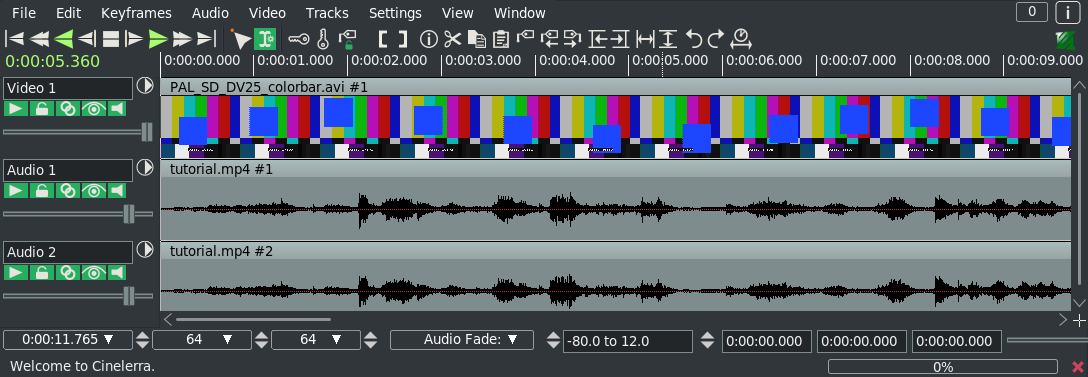
\includegraphics[width=1.0\linewidth]{patchbay.png}
    \caption{Patchbay  | Timeline with pulldowns, navigation icons, Video/Audio tracks | bottom Zoom Panel}
    \label{fig:patchbay}
\end{figure}

Video tracks represent the duration of your media, just as if you placed old-fashioned rolls of photographic
film one right after the other on a table.
Individual images that are drawn on each track are snapshots of what is located at that place on the timeline.

Audio tracks represent the sound media as an audio waveform, or if you change a preference setting, a rectified audio waveform. 
This too looks like old-fashioned digital magnetic tape laid out horizontally across a table.
Using the \textit{Zoom Panel} controls at the bottom of the timeline,
you can adjust the horizontal and vertical size of the video and audio waveform displays.
Each track on the timeline has a set of attributes on its left side in the patchbay which is used to 
control some options of that particular track. 

Track Navigation is performed by selecting a video or audio track and moving to a certain time in the track. 
Use the vertical scroll bar to scan across tracks, or even easier you can use the mouse wheel. 
And use the horizontal scroll bar to scan across time, or again even easier, you can use the mouse wheel with the Ctrl key.  

Once you have become familiar with many of the graphical tools and pulldowns, you can switch to using more of
the keyboard to navigate.  Many of the key equivalences are listed in each of the pulldowns to the right of the option
 as a shortcut. All of the shortcuts are listed in a document for keyboard 
navigation (\ref{sub:main_menu_keys}). This includes, for example, shortcuts like the \texttt{Home} and \texttt{End} keys to go to the beginning or end of the timeline.  
Another example is in the default cut and paste mode, hold down \texttt{Shift} while pressing \texttt{Home} or \texttt{End} in order to select the region of the timeline between the insertion point and the key pressed.

\subsection{Zoom Panel}%
\label{sub:zoom_panel}

Below the displayed tracks in the timeline, you will find the zoom panel as seen in figure~\ref{fig:patchbay}.
In addition to the scrollbars, these options and their values are another set of tools for positioning the timeline.  
In order of appearance in the zoom panel as rectangular boxes and either tumbler arrows or a up/down arrow, this next list shows each option along with its tooltip description if available.
Then more details are provided in the next paragraphs.

\vspace{2ex}
\begin{tabular}{ll}
   \hline
	Sample zoom & Duration visible on the timeline \\
	Amplitude & Audio waveform scale \\
	Track audio zoom & Height of audio tracks \\
	Track video zoom & Height of video tracks \\
	  (type) & Automation Type \\
	Curve zoom & Automation range minimum and maximum \\
	Selection change & 3 boxes with starting point, length, and ending point \\
	Alpha slider & Slider bar to control alpha value for colored assets \\
   \hline
\end{tabular}

Changing the \emph{sample zoom} changes the amount of time displayed on the timeline 
so you can see your media as individual frames or as the entire length of your media. 
To see more frames, use a higher setting. 
The sample zoom value is not an absolute time reference because it refers to the duration visible on the timeline. It will change as you modify the length of the program window horizontally.
You can either use the $\uparrow$ and $\downarrow$ arrows to change the sample zoom by a power of two, or use the mouse wheel on the tumblers to zoom in and out.


The next option is \emph{amplitude} and it only affects the audio waveform size. \texttt{Ctrl-$\uparrow$} and \texttt{Ctrl-$\downarrow$} are shortcuts used to change the amplitude zoom as an alternative to the down arrow to the right of the numerical size.

The \emph{track audio and video zoom} affects all tracks of that type and determines the height of each track. 
If you change the audio track zoom, the amplitude zoom will be changed also so that the audio waveforms
are proportionally sized.
Shortcuts, \texttt{Ctrl-Pgup} and \texttt{Ctrl-Pgdown}, change the track zoom to the next level simultaneously for all of the audio and video tracks.

\emph{Automation type} is used for selecting one of the following: Audio Fade, Video Fade, Zoom, Speed, X, or Y (X and Y are for the compositor's Camera and Projector).  When an auto line is present on
the timeline and is being manipulated, a small square the same color as the line will be shown to 
the left of the Automation type.  This is just an indicator to make it easy to see what is being worked.
 
The \emph{curve zoom} affects the curves for the selected \emph{automation type} in all the tracks of that type and determines the value range for those curves. 
Use the tumbler arrows to the left of the numbers for the minimum value and the tumblers to the right for the maximum value, or manually enter the values in the text box. 
Good default values for audio fade are -40.0 to 6.0 and for video fade are 0.0 to 100.0. 
The tumbler arrows change curve amplitude, but the only way to curve offset is to use the fit curves button on the curve itself.

The \emph{selection start time}, \emph{selection length}, and \emph{selection end time} display the current selected timeline values. When there is no selection, both the start and end time are the current
position of the timeline and the selection length is 0.
The \emph{alpha slider} allows for varying the alpha value when using colors on the tracks as set in your \texttt{Preferences $\rightarrow$ Appearance} for \texttt{Autocolor assets}.  
It has no function without that flag set.

There are 3 additional pieces of information in the line immediately below the \textit{zoom panel}.
In the lower left hand corner there could be messages such as "Welcome to \CGG{}" when there is no 
need to display a red-colored error message or a line that reads "Rendering took H:MM:SS" after a render
has just been completed. Or when working with an auto, a small square the color of that auto line, will be
present along with its keyframe type, location on the timeline, and its current value.  This is simply
for easy recognition of what is being worked. The second piece of helpful information is all the way to
the right which is a long rectangular box indicating the percentage completion of a render. Finally
there is an X with the tooltip of "Cancel operation" used to stop an ongoing render
(the cancel operation may seem slow due to the amount of data still in the buffer upon cancellation).

\subsection{Track Popup Menu}%
\label{sub:track_popup_menu}

Each Track has a popup menu. 
To activate the track popup menu, Right mouse click (RMB) on the track. 
The popup menu affects the track whether the track is armed on the patchbay or not. 
The Track Menu contains a number of options:

\begin{description}
    \item[Attach Effect] opens a dialog box of effects applicable to the type of track of audio or video.
    \item[Move up] moves the selected track one step up in the stack of its corresponding type - audio or video.
    \item[Move down]  moves the selected track one step down in the stack of its corresponding type - audio or video.
    \item[Delete track]  removes the track from the timeline.
    \item[Add Track]  adds a track of the same media type as the one selected, audio or video, above the selected track.
    \item[Find in Resources]  that media file will be highlighted in the media folder in the Resources window. If the 
	Resources window is closed, media is found and highlighted but the Resources window is not displayed.
    \item[Show edit]  will point out the exact start and stop points along with the length of the current edit on
        that track as well as the media name, track name and number, and edit number.
    \item[User title]  is used to change the title name.  This is really handy for files that have very long and
        similar names that would get cut off during edits.  You can use short names to better differentiate the
        media. In Drag and Drop editing mode, if you select multiple edits all of those clips will have
their title name changed.
    \item[Bar color]  allows the user to select a specific color for the title bar.  This helps to more easily locate a piece of media.
    \item[Resize Track]  resizes the track; this is only applicable to video tracks.
    \item[Match Output Size]  resizes the track to match the current output size; this is only applicable to video tracks.
\end{description}


\subsection{Insertion Point}%
\label{sub:insertion_point}

The insertion point (figure~\ref{fig:insertion-points}) is the vertical hairline mark that spans the timeline in the program window - it can be a solid line but most of the time it will be flashing. 
Like the cursor on a word processor, the insertion point marks the place on the timeline where the next
operation will begin. It is the starting point of all play operations and is the point where a paste operation will occur. 
In some cases, when rendering it defines the beginning of the region of the timeline to be rendered. 

To move the insertion point, you move the mouse inside the timebar area and click with the left mouse button. 
You can use any place on the timebar to reposition the insertion point as long as that spot is not blocked
by In/Out point or a label. 
In cut and paste editing mode, you can also change the position of the insertion point with a simple 
left mouse click in the timeline itself.
When moving the insertion point, the position is either aligned to frames or aligned to samples. 
For best results, \textit{Align cursor on frames} when editing a video track and \textit{Align to samples} when editing audio. 
Use the pulldown \texttt{Settings$\rightarrow$Align cursor on frames} to change the alignment by
checking the box on for video and off for audio.

\begin{figure}[htpb]
    \centering
    %\includegraphics[width=0.8\linewidth]{name.ext}
    \begin{tikzpicture}[scale=1, transform shape]
        \node (img1) [yshift=0cm, xshift=0cm, rotate=0]
         {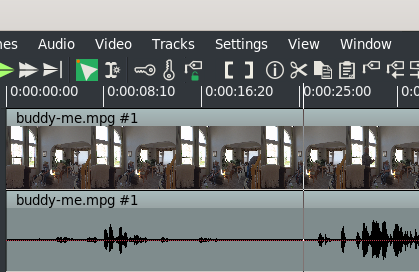
\includegraphics[width=0.6\linewidth]{insertion-point.png}};
        \node [yshift=-5mm, xshift=-1cm,anchor=east] at (img1.north west) (Pulldowns) {Pulldowns};
        \node [yshift=-10mm, xshift=-1cm,anchor=east] at (img1.north west) (Transport) {Transport \& Buttons Bar};
        \node [yshift=-15mm, xshift=-1cm,anchor=east] at (img1.north west) (Timebar) {Timebar};
        \node [yshift=-20mm, xshift=-1cm,anchor=east] at (img1.north west) (Title) {Media Title };
        \node [yshift=-28mm, xshift=-1cm,anchor=east] at (img1.north west) (Video) {Video Track};
        \node [yshift=-46mm, xshift=-1cm,anchor=east] at (img1.north west) (Audio) {Audio Track};
        \draw [->, line width=1mm] (Pulldowns) edge  ([yshift=-5mm] img1.north west);
        \draw [->, line width=1mm] (Transport) edge  ([yshift=-10mm] img1.north west);
        \draw [->, line width=1mm] (Timebar) edge    ([yshift=-15mm] img1.north west);
        \draw [->, line width=1mm] (Title) edge      ([yshift=-20mm] img1.north west);
        \draw [->, line width=1mm] (Video) edge      ([yshift=-28mm] img1.north west);
        \draw [->, line width=1mm] (Audio) edge      ([yshift=-46mm] img1.north west);
        \end{tikzpicture}
    
    \caption{Insertion point is at 0:00:25:10 in Hr:Mn:Sec:Frames}
    \label{fig:insertion-points}
\end{figure}


\subsection{Editing Modes}%
\label{sub:editing_modes}

There are 2 different editing modes for operations which affect how the insertion point and editing
on the timeline operate.  
There is:  \emph{drag and drop mode} and \emph{cut and paste mode}. 
The editing mode is determined by selecting the \texttt{arrow}, or immediately to the right of the arrow,
the \texttt{I-beam} in the Transport and Buttons bar. In figure~\ref{fig:insertion-points} you can see
the green colored highlight \protect\footnote{green is used in the default Cakewalk theme, but the highlight color will be different in other themes} on the arrow icon indicating that you are currently in 
\emph{drag and drop mode}.

With the arrow highlighted for \emph{drag and drop mode}, a double click with the left mouse button in the timeline selects the edit the mouse pointer is over. 
Then dragging in the timeline repositions that edit and this can be used for moving effects,
changing the order of playlists, or moving video pieces around. 
There are numerous methods to cut and paste in \emph{drag and drop mode} by setting In/Out points to define
a selected region or using the Copy/Paste Behavior as outlined in~\ref{sub:copy_paste_behavior}. 
In this mode, clicking the LMB in the timeline does not reposition the \textit{Insertion Point}. 

When the I-beam is highlighted, you are in \emph{cut and paste mode}.
In cut and paste mode, clicking the LMB in the timeline does reposition the \textit{Insertion Point}. 
Double clicking in the timeline selects the entire edit the cursor is over, i.e.\ that column. 
Dragging in the timeline with the LMB pressed down, highlights a selected region and this is the region that is affected by cut
and paste operations.  It is also the playback range used for the subsequent playback operation. 
Holding down the Shift key while clicking in the timeline extends the highlighted region.

\begin{figure}[htpb]
    \centering
    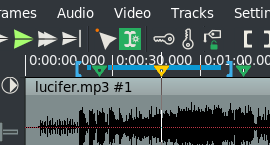
\includegraphics[width=0.4\linewidth]{i-beam.png}
    \caption{I-beam + in/out  +  labels}
    \label{fig:i-beam}
\end{figure}

\subsection{In/Out Points}%
\label{sub:in_out_points}

The In/Out points, displayed on the timebar by [ and ] brackets,  can be set in either of the editing modes to define the selection.
In the timebar, a colored bar will show between these 2 brackets to better outline the area selected.
In \emph{drag and drop mode}, they are an easy way to define a selected region.

It is important to remember that in \emph{cut and paste mode} and \emph{drag and drop mode}, a highlighted area 
overrides the In/Out points. That is, if a highlighted area and In/Out points are both set, the highlighted area is changed by editing operations and the In/Out points are ignored. 
But if no region is highlighted, the In/Out points are used. 
To avoid confusion, use either highlighting or In/Out points but not both at the same time.

To set In/Out points, in the timebar move to the position where you want the In point and click the In
point icon or one of the [ or < keys.
Then move the insertion point to a position after the In point and click the ] or > or the Out point icon. 
You can use these same icons or keyboard characters to toggle In/Out points on or off.

If you set the insertion point in another place when In/Out points are already set, that existing point will be
repositioned when you click the In/Out icon or keyboard equivalent. 
If you click on In/Out points while a region is highlighted, the insertion point will be ignored and In/Out points will be set at the beginning and at the end of the highlighted area.

When you select either the In or Out point on the timebar, the insertion point will move to that location.Note that when the insertion point is at the exact position of an In or Out point, the bracket will change
color making it easy to see that you are exactly at that spot.
 
If only the In point is set, when you click the In point icon the In point will be deleted. 
If only the Out point is set, when you click the Out point icon the Out point will be deleted. 
Holding the Shift key while clicking on an In/Out point, the area between the insertion point and that
In/Out point will be highlighted or extended to that In/Out point if already highlighted. 

An easy way to turn off the In/Out points if both are set, is to double click on the [ icon in the toolbar. 
If you have already set the In and Out points, and then move the insertion point anywhere to the left of
the Out point, a LMB click on the [ icon will move the In point to the location of the insertion point.  In the same
manner if you move the insertion point anywhere to the right of the In point, a LMB click on the ] icon
will move the Out point to that new position.  However, if you move the insertion point for either the
In or Out point beyond what makes sense to designate In/Out points, the bracket you clicked on will be
moved to the insertion point and the other bracket will be eliminated.  That is obviously because the
In point has to come before the Out point on the timeline.

Some of the useful operations concerning the In/Out pointers are listed next.

\begin{description}
    \item[Ctrl-KeyPad\#]  if In/Out set, \texttt{KP 2,3,5,6 + Enter}, play between In/Out points
    \item[Shift-Ctrl]  loops play between In/Out points
    \item[Click In/Out] while holding the LMB down, drags In/Out pointer where you drag to
    \item[Shift-Ctrl] with a transport button (e.g. Fast Forward), loops play between In/Out points
    \item[Ctrl-t]  clears both In/Out points
\end{description}

\subsection{Labels}%
\label{sub:labels}

Labels are used in order to set exact locations on the timeline that you want to be able to easily get to. 
To create a label, position the insertion point at a location and click on the label icon in the Transport
and Buttons bar. The new label is displayed on the timebar as a down arrow at that location as shown in
figure~\ref{fig:i-beam}.  Whenever the insertion point is at the same position as a label, it changes
color to emphasize that it is exactly at that spot.
Labels make it so you can jump back and forth to exact marked locations on the timeline.
Use the lower case letter “\texttt{L}” as a shortcut for the label button.

You can use labels to reposition the insertion point when that label is selected. They are also
especially useful for moving along the timeline to the \textit{Next label} or \textit{Previous label}
with the buttons on the Transport and Buttons bar to the right of the Labels button.  
When moving along the timeline with the Next or Previous label buttons, if a label is out 
out of view the timeline will automatically be repositioned so that the label is visible.
If you perform a \textit{Next label} operation and there are no more, the insertion point
will go to the End position.  Conversely if you perform a \textit{Previous label} operation
and there are no more labels, the insertion point will go to the Home position. 
Keyboard shortcuts for label traversal are:

\begin{description}
    \item[Ctrl-left] moves the insertion point to the previous label.
    \item[Ctrl-right] moves the insertion point to the next label.
\end{description}

There is a  Label folder in the Resources window which has a list of every label and its exact location
where the label is. The location is based on the timestamp, frame number, or sample number depending on the selected Time Format of your timebar. 
You can edit, delete, or goto a label by clicking the RMB on that label in the Resources window which
brings up a popup menu with those options.  It can be quite helpful to \textit{edit} the label
and add a text string to help identify what the label represents.
In addition, RMB clicking the label symbol on the timebar brings up a textbox displaying the current
text string and allowing you to change it. If a Label has been given a name, simply mousing over
the label symbol on the timebar will display that string.

With labels you can also select regions:

\begin{description}
    \item[Shift-Ctrl-left] highlights the area between the insertion point and the previous label.
    \item[Shift-Ctrl-right] highlights the area between the insertion point and the next label.
    \item[Double-clicking] on the timebar between two labels, highlights the area between the labels.	   
    \item[Shift-clicking] on a label, highlights the area between that label and the insertion point.
        If an area is already highlighted, it extends the highlighted area up to that label.
\end{description}

If you LMB click the label button when an area is highlighted, labels are created at each end of the
highlighted area. 
When a label is selected, if you click on the label icon, the label will be deleted. 
To delete multiple labels, highlight that area, then use the \texttt{Edit $\rightarrow$ Clear $\rightarrow$ Clear labels}
function to delete them all. The same precedence rules apply to this operation as mentioned earlier.  That
is, if both In/Out points are set and there is a highlighted area also set, the highlighted area's 
labels will be cleared and not those between the In/Out points.

If you enable \emph{Edit labels} in the Settings pulldown menu or disable the \emph{Lock labels from moving}
button on the Transport and Buttons bar, labels will be cut, copied or pasted along with the selected
area of the first armed track. 
In the same manner, if a selected area of media is spliced from the viewer to the timeline in a position 
before labels, the labels will be moved to the right on the timebar so that the label maintains its 
relative position to its edit. 
To prevent labels from moving on the timebar, enable the \emph{Lock labels from moving} icon or
disable the \emph{Edit labels} option under the Settings pulldown.

\subsection{Color Title Bars and Assets}%
\label{sub:color_title_bars_and_assets}

In order to visually aid in locating clips on the timeline that are from the same media file, you can have them auto-colored or self-colored.  
Use of this feature requires additional memory and cpu on every timeline redraw, therefore it is recommended that smaller computers leave it turned off.

For auto-color the color will be based on a hashed filename so that whenever you load this particular media, it will always have the same color on the title bar even if you use proxy.  
To enable auto-color go to \texttt{Settings $\rightarrow$ Preferences, Appearance tab} and check on \texttt{Autocolor assets}. You will see this in the Flags section
as shown in Figure~\ref{fig:settings}.  It is disabled by default.  
Each media will have a random muted color and there could easily be close duplicates as generated by the program algorithm.  There will be no total black, but some dark shades are possible.  

To change a specific clip to your own chosen color, right mouse button (RMB) over that clip and an Edits popup will be displayed.  
Choose the option \textit{Bar Color} to bring up the color picker and choose a color.   
You can also change the alpha value in the color picker and this alpha takes precedence over the current alpha slider bar value unless the color picker's alpha value is set to 1.0.   
The color will only change after you click on the checkmark.  
The \emph{Bar Color} option works in either Drag and Drop or Cut and Paste editing mode and also works if \textit{Autocolor assets} is not set.  
In Drag and Drop editing mode, if you select several clips and then bring up the Edits popup with the right mouse button over a track, you can use the \emph{Bar Color} option to change all of those selected to the same color.

To go back to the default colors, uncheck \textit{Autocolor assets} in Preferences, but this does not affect the specially chosen self-colored ones as they are preserved.  
To change these individually or  selectively, use the Edits popup \emph{Bar Color} option and click on \textit{Default} in the color picker window.  Auto-color does not honor armed/disarmed tracks.  
Self-color does honor armed/disarmed tracks.

And that’s not all!  
There is an \emph{alpha fader slider bar} on the bottom of the main window on the right hand side of the Zoom Panel.  
With this alpha slider, you can colorize your video and audio tracks to either see only the color at 0.0 or see only the image at 1.0.  
This slider bar affects all colored areas of the Autocolor assets and the self-colored ones.  
In the case when a specifically changed edit alpha value is set in the color picker
to any value except 1, the slider bar will not affect that.  
Once you use the slider bar, it is activated so gets first shot at any keystrokes in the main window.  
You deactivate this by simply clicking in a different part of the main window.  

As long as we are on the subject of color, just a note that you can also change the \textit{Highlighting Inversion color} in \texttt{Settings $\rightarrow$ Preferences, Appearance tab}.  You can see this option in Figure~\ref{fig:settings} in the Color section.  
That setting defaults to white ($ffffff$) but sometimes this is a little bright so you can put any hex value in that suits you.

This image (figure~\ref{fig:autocolor_assets_alpha}a) shows an example of the Autocolor assets with alpha set to 0.0 so that you see only the color and no image.
In this image (figure~\ref{fig:autocolor_assets_alpha}b), the alpha is set to show the image
and waveforms with transluent colors.  The pink media file has been self-colored rather than the autocolor to make it easy to see.

\begin{figure}[htpb]
    \centering
    \begin{minipage}[h]{0.55\linewidth}
        \center{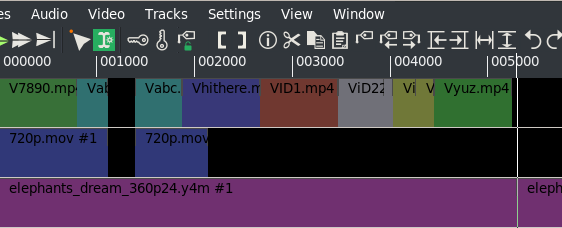
\includegraphics[width=0.99\linewidth]{autocolor-assets_alpha0.png}} \\ a)
    \end{minipage}
    \begin{minipage}[h]{0.4\linewidth}
        \center{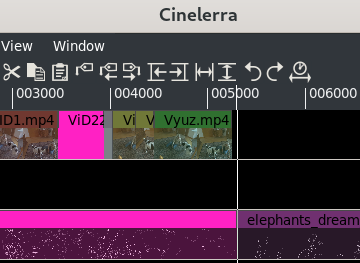
\includegraphics[width=0.99\linewidth]{autocolor-assets_alpha1.png}} \\ b)
    \end{minipage}
    \caption{An example of the Autocolor assets}
    \label{fig:autocolor_assets_alpha}
\end{figure}


\subsection{More about Pulldowns}%
\label{sub:more_about_pulldowns}

The main window pulldowns as pointed out in figure~\ref{fig:insertion-points} are quite obvious in their meaning and usage, so here is only a summary.  

%TODO Figure 3 shows an example of the pulldowns as displayed in the main window.Appearance


\begin{description}
    \item[File]  options for loading, saving, and rendering as described in other sections (\ref{cha:load_save_and_the_EDL}).
    \item[Edit]  edit functions; most of which have shortcuts that you will quickly learn (\ref{cha:editing}).
    \item[Keyframes]  keyframe options which are described in the Keyframe section (\ref{cha:keyframes}).
    \item[Audio]  audio functions such as \textit{Add track}, \textit{Attach effect}
and \textit{Attach transition}.  The \textit{Attach effect} is especially useful when
you need the effect to be applied to all related audio tracks as a \textit{Shared effect}
and is described as an alternative method of application in section \ref{sec:shared_effect_tracks}.
    \item[Video]  video functions such as \textit{Add track, Default/Attach transition, Render effect}.
    \item[Tracks]  move or delete tracks are the most often used.
    \item[Settings]  much of this is described elsewhere with the most frequently used to include
Preferences (\ref{cha:configuration_settings_preferences}), Format (\ref{cha:project_and_media_attributes}), 
Proxy and Transcode (\ref{sec:proxy_settings}), as well as the others.
    \item[View]  for display or modifying asset parameters and values to include Fade, Speed, and Cameras.
    \item[Window]  window manipulation functions.
\end{description}


\subsection{Window Layouts}%
\label{sub:window_layouts}

If you like to use different window layouts than the default for certain scenarios, you can setup, save, and load 4 variations.   
First, position your \CGG{} windows where you want them to be and then use the Window pulldown and choose \emph{Save layout}. Note the words \emph{Save layout} highlighted in Figure~\ref{fig:window_layouts}a with 4 names shown to the right and below of that highlight. 
To use the default name of \textit{Layout \#}, when the popup comes up, just click the green checkmark OK on the Layout popup menu.  
If you would like a specific name for your layout so you can remember what its best use case is,
keyin 1-8 english characters that are meaningful to you (english characters mean you can not use the German umlaut, the French accent, or the Spanish ñ). 
Legal characters are a-z, A-Z, 0-9, \_ (the underscore character) and a limit of 8 total.  
If you keyin more than 8, only the last 8 characters will be used.  
To rename a currently existing layout, use the \emph{Save layout} option again on the one to rename, and keyin a different name into the text box or leave blank for the default name (figure~\ref{fig:window_layouts}b).

\begin{figure}[htpb]
    \centering
    \begin{minipage}{.49\linewidth}
        \center{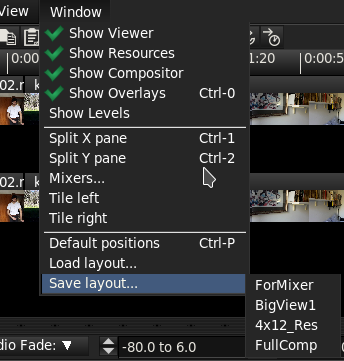
\includegraphics[width=1\linewidth]{window_layout1.png}}\\ a)
        %TODO High res image replace
    \end{minipage}
    \begin{minipage}{.49\linewidth}
        \vspace{13ex}
        \center{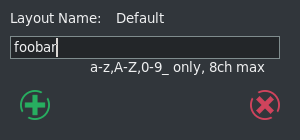
\includegraphics[width=1\linewidth]{window_layout2.png}}\\ b)
        %TODO Alpha channel
    \end{minipage}
    \caption{Window Layouts}
    \label{fig:window_layouts}
\end{figure}

The files containing the coordinates for your layouts will automatically be saved in the \texttt{\$HOME/.bcast5} directory as \texttt{layout\#\_rc} or \texttt{layout\#\_8chars\_rc}.

To use the desired layout, keyin the shortcut or use the Window pulldown and choose \emph{Load layout} and then make your choice. It is very beneficial to learn the shortcuts for your
layouts because they can be executed from any of the 4 windows instead of just the main
timeline window.

\subsection{Just Playing!}%
\label{sub:just_playing_}
What if you are just using \CGG{} to play media and listen to tunes? 
After loading your media, just hit the space bar to start playing and then again to stop playing.  
Other than that, use the transport buttons on the top bar of the Program window.  
Other ways to \textit{play around} are described next. 

\subsubsection*{Repeat Play / Looping Method}%
\label{ssub:repeat_play_looping_method}

There are 2 methods for repeat play or looping on the timeline and 1 method for both the Compositor and the Viewer.  This works in conjunction with any of the transport buttons or shortcuts in either forward or reverse as usual.  The 1 exception is that the Shift key can not be used to either add or subtract audio within the repeat area.

\textit{Method 1:} Shift-L on the Timeline, repeats the selection per the algorithm outlined next.
  
When setup, long green lines are displayed across the entire set of tracks which shows the start and end of the loop.
\begin{enumerate}
    \item  Highlighted selection repeats loop and takes precedence over all other possibilities.  
        If the cursor is before the highlighted area, it will play up to the area and then repeat the highlighted section.  
        If the cursor is after the highlighted section, play will start at the beginning until you get to the
        highlighted section and then repeat.
    \item  When both In and Out pointers are set, it repeats the section between [ and ].
    \item  If only one of the In or Out pointers is set, it loops the whole media.
\end{enumerate}

\textit{Method 2:} Ctrl+Shift+transport button on the Timeline, Viewer, and Compositor

\begin{enumerate}
    \item Repeats entire media if no In or Out pointer set.
    \item  In and Out pointer set, repeats area between pointers.
    \item  Only In pointer set, repeats from In to end of media.
\end{enumerate}

\subsubsection*{Last Play Position Memory}%
\label{ssub:last_play_position_memory}


When you play media, the start/end playback positions are saved as if they had been made into temporary labels.  
They appear on the timeline as purple/yellow hairline markers representing the last start/end labels for the last playback. 
They can be addressed as if they are label markers using:

\begin{description}
    \item[Ctrl$\leftarrow$]   tab to the label before the cursor, that is \textit{play start}
    \item[Ctrl$\rightarrow$]   tab to the label after the cursor, that is \textit{play stop}
\end{description}


You can use these markers for re-selection.  
Additionally, the selection region can be expanded by \textit{pushing} the markers using single frame playback.  
Use frame reverse (\texttt{keypad 4}) to push the start play marker backward, or use frame forward (\texttt{keypad 1}) to push the end play marker forward.

Another handy feature is to use the combination of Ctrl-shift-arrow (left or right) to select the media from the cursor position (red hairline) to the start or end marker by \textit{tabbing} to the label markers.  
For example, tab to the beginning of the previous play region using Ctrl-left-arrow to move the cursor to the beginning of last play, then press Ctrl-Shift-right-arrow to tab to the end of the playback region. 
Now you can clip/play/expand or edit the previous playback selection.

\begin{description}
    \item[Ctrl SHIFT$\rightarrow$] 	  tab cursor to label right of cursor position and expand selection
    \item[Ctrl SHIFT$\leftarrow$] 	  tab cursor to label left of cursor position and expand selection
\end{description}


\subsubsection*{Playback Speed Automation Support}%
\label{ssub:playback_speed_automation_support}


The speed automation causes the playback sampling rate to increase or decrease to a period controlled by the speed automation curve.  
This can make playback speed-up or slow-down according to the scaled sampling rate, as \textit{time is multiplied by speed} (Speed $\times$ Unit\_rate). For more information on changing
the speed, read the section on Speed Automation~\ref{sec:speed_fade_automation_gang}.

\subsubsection*{Alternative to using Numeric Keypad for Playing}%
\label{ssub:alternative_to_using_numeric_keypad_for_playing}


For the keyboards without a numeric keypad or if you prefer to use keys closer to where you normally type, there are alternative keys for the play/transport functions.  These are listed below.

\begin{tabular}{lcl}
	Alt + m&=&stop playback\\

	Alt + j&=&forward single frame\\

	Alt + k&=&forward slow playback\\

	Alt + l&=&forward normal playback\\

	Alt + ;&=&forward fast playback\\

	Alt + u&=&reverse single frame\\

	Alt + i&=&reverse slow playback\\

	Alt + o&=&reverse normal playback\\

	Alt + p&=&reverse fast playback\\
\end{tabular}
\begin{minipage}{.45\linewidth}
+ Shift key, results in the reverse of whether audio is included or not.
\vspace{1ex}

+ Shift + Ctrl, results in the transport function operating only between the in/out pointers.
\end{minipage}

\section{Compositor Window}%
\label{sec:compositor_window}

\begin{figure}[htpb]
    \centering
    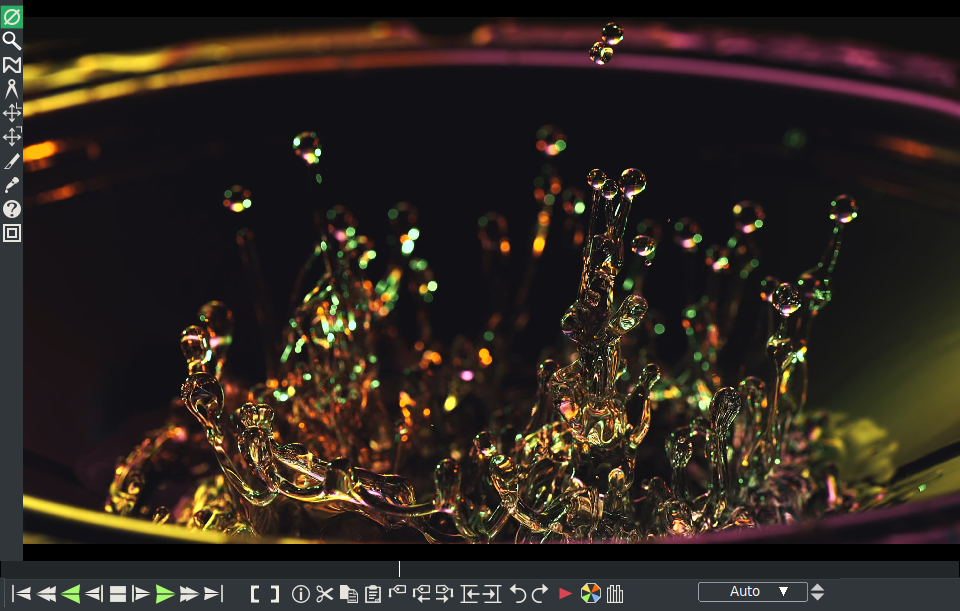
\includegraphics[width=0.99\linewidth]{compositor_window.png}
    \caption{Left hand side are the toolbar functions / bottom bar has many control functions}
    \label{fig:compositor_window}
\end{figure}

The Compositor window (figure~\ref{fig:compositor_window}) is used to display the timeline
output.  Playing and moving along the timeline video in the Program window shows in the
Compositor window what the current image is.  Here is where many compositing operations are
performed that can change 
what the timeline will look like.  When enabled, you can simply click the LMB in the Compositor
window to start and stop play.
  You can zoom in and out to 
see small details, pan with the scrollbars, lock the window to prevent changes, add masks,
and make changes with the Projector and Camera function operators. These will be explained
in more detail in the following sections.

\subsection{Compositor Controls}%
\label{sub:compositor_controls}

On the bottom of the window, there are many
of the same transport buttons and controls that are available in the Program window.
They work the same as in the Program window and also have tooltips that are visible 
when you mouse over each of the icons so their use is fairly obvious.  However,
of particular note is the button \textit{Click to play} which is described in~\ref{sub:click_to_play_in_viewer_and_compositor}.  Next is the \textit{Videoscope} button which is used to enable the scopes window
without having to apply the filter to the tracks/edits.

Next to all of these controls all the way to the right side, there is a \textit{zoom menu} and a \textit{tally light}.  The \textit{zoom menu} has a pulldown with different settings that you can choose from
or you can just use the tumbler arrows to the right. Generally when just getting started, you
will be using the default \textit{Auto} option.  The window size is not changed, but rather
the size of the video itself. In addition there are many shortcuts for zooming that you
will find in the Shortcuts chapter (\ref{cha:shortcuts}).

To resize the entire window instead of just the video, use a RMB click in the compositor
window which brings up a menu with all the zoom levels, zoom auto mode, and some other options. 
As you would expect, whenever the video is zoomed so that only part of the image is visible
in the window, scrollbars are automatically added as needed on the bottom, the right hand 
side, or both.
Other options include \emph{Reset camera} and \emph{Reset projector} which obviously are used
to reset the camera and the projector. 
The \emph{Hide controls/Show controls} option is great for hiding the left hand toolbar and
bottom set of controls for a cleaner look. 

Next to the zoom tumbler arrows, is a \textit{tally light} that will be filled in with some color
(often red or blue) when a rendering operation
is taking place. This is especially helpful when loading a very large video so you know
when it is finished loading.  You should pay attention to this \textit{tally light} when performing
a particularly time-consuming operation so that you do not keep executing more operations
that just have to wait until completion of that CPU intensive operation.  Also, you should look
to see if the light is on before assuming that \CGG{} is hung up.

When the window is unlocked, meaning that it is not in \textit{Protect video from changes} mode on the
toolbar, MMB clicking and dragging anywhere in the video pans the view.  Panning can also
be accomplished with the bottom and right hand side scroll bars when displayed.

\subsection{Compositor Toolbar}%
\label{sub:compositor_toolbar}

On the left hand side of the Compositor window, there is a toolbar with several icons that
provide functions for viewing and compositing the video. Each of these operational features 
will be described in more detail next. 
\begin{description}
    \item[Protect video from changes] this option makes it possible to disable changes to the
compositor output when clicking on the Compositor window. It allows for using the
\textit{Click to play} button (when enabled) for simply starting and stopping play.  It helps
to prevent an accidental click from making unwanted changes. When you enable this option, any
of the other enabled tools will automatically be disabled.

     \item[Zoom view / magnifying glass] when enabled, the \textit{Zoom view} immediately results
in the addition of a zoom slider for fine viewing.  
The vertically oriented \textit{zoom slider} will be displayed underneath the last icon of the toolbar and extends
to almost the end of the toolbar.
The slider allows for adjusting the amount of zoom at any level between 0.01 and 100 based on a logarithmic scale.  

When using the zoom slider, the number by which the view is zoomed can be seen in the textbox 
on the bottom controls where the \% zoom is located.  
The zoom slider size is in the form of \textit{times}, such as $\times$0.82 which indicates that the picture is zoomed to $\frac{82}{100}^{th}$ of the original size as seen in the \texttt{Settings $\rightarrow$ Format} menu.  
Once you have set the zoom to the desired size, use the vertical and horizontal scroll bars to position the view as needed.
As mentioned earlier, this
variety of zoom only affects the video and not the resizing of the Compositor window.  After
utilizing this slider bar for zooming around, you may want to switch back to \textit{Auto} 
using the Controls on the bottom of the window.
This slider bar is also displayed
when you click on the icons for \textit{Adjust camera automation} or \textit{Adjust projector automation}.  

The Compositor window image in figure~\ref{fig:zoom_slider} shows the zoom slider bar with rectangular shaped slider about in the middle.  Note that the magnifying glass is enabled which
automatically pops-up the slider and the Protect video from changes is disabled.  Also note that
there is a scroll bar on the bottom and right side of the image since the image at this magnification
does not fit in the window.
The Controls zoom textbox shows $\times0.82$ size.  
\end{description}

\begin{figure}[htpb]
    \centering
    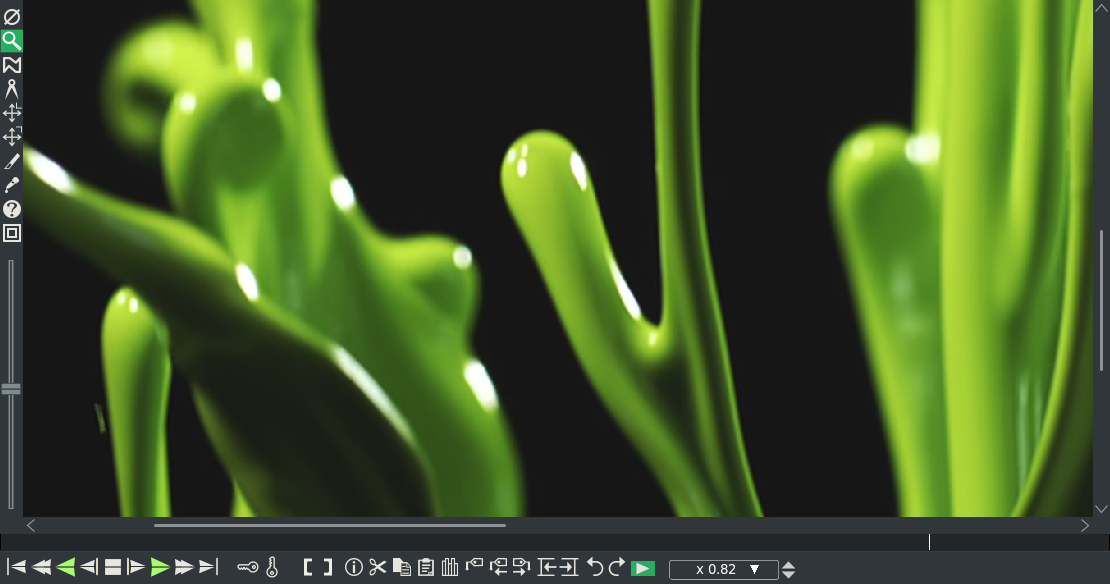
\includegraphics[width=0.99\linewidth]{zoom_slider.png}
    \caption{Compositor window zoom slider bar and scroll bars}
    \label{fig:zoom_slider}
\end{figure}
\begin{description}
    \item[Edit mask] brings up a mask editing menu with many versatile options as
described in great detail later in this section (\ref{sub:masks}). You may also have to click on
\textit{Show tool info} to popup the menu depending on whether or not you dismissed that window previously.
    \item[Ruler] this can be a handy tool to get the X,Y coordinates of an exact point or to 
measure the distance between 2 points. To use the \textit{Ruler}, move the mouse on the video to
get to the desired spot - these X,Y coordinates will be displayed in the \textit{Current} text
box.  Clicking the LMB creates Point 1 and then continue to hold down the LMB so that a ruler line is created between
this Point 1 and the stopping Point 2.  \textit{Deltas} is the X,Y difference between the 2 points;
\textit{Distance} is the number of pixels between the 2 points; and \textit{Angle} is the angle in degrees of the ruler line.  
In Figure~\ref{fig:safe_regions} you can see the Ruler menu on the right side of the Compositor window.

Holding down the Ctrl key while dragging with the LMB on one of the points, will
ensure that the line is always at a multiple of a 45 degree angle.  Holding down the Alt key while
dragging with the LMB on any of the points, will translate the ruler line to another place on 
the video while maintaining its length and angle. For some desktop window managers, such as 
\textit{UbuntuStudio 16.4} and \textit{Arch}, the Alt key is already in use by the Operating System
so you will have to use Alt+Ctrl instead.
If you dismiss the Ruler menu, click on
\textit{Show tool info} to get the menu to popup again.  
    \item[Adjust camera automation]  the camera brings up the camera editing tool. Enable \textit{Show tool info} if the popup menu does not appear. More detail for usage is provided in the subsequent
section~\ref{sub:camera_and_projector}.
    \item[Adjust projector automation]  the projector brings up the projector editing tool. Enable \textit{Show tool info} to get the menu to popup again. More detail for usage is provided in the
subsequent section~\ref{sub:camera_and_projector}.
    \item[Crop a layer or output]  this is a cropping tool used to reduce the visible picture area.
More detail for usage is provided in a 
subsequent paragraph (\ref{sub:cropping}).  There is also a Crop \& Position plugin that provides
a different set of capabilities~\ref{sub:crop_position}.
    \item[Get color / eyedropper]  brings up the eyedropper used to detect the color at a
particular spot.  Enable the \textit{Show tool info} if the Color popup menu does not come up 
automatically or if that menu was accidentally dismissed.  Click on a specific color in the video
output with the LMB to see the selected color. You can then use that color's 
value to be applied to some effects depending on how the effect handles the eyedropper.
    \item[Show tool info]  this tool button is used in conjunction with the other tools on the
compositor's toolbar. You only need to click on this if one of these tools popup menu does not
come up or has been dismissed - Mask, Ruler, Camera, Projector, Crop, or Eyedropper tools.
You can also use it when highlighted to dismiss the highlighted tool's dialog box.
It is not needed for Protect video from changes, Zoom view, and Show safe regions since they have
no dialog popup menus.

\begin{figure}[htpb]
    \centering
    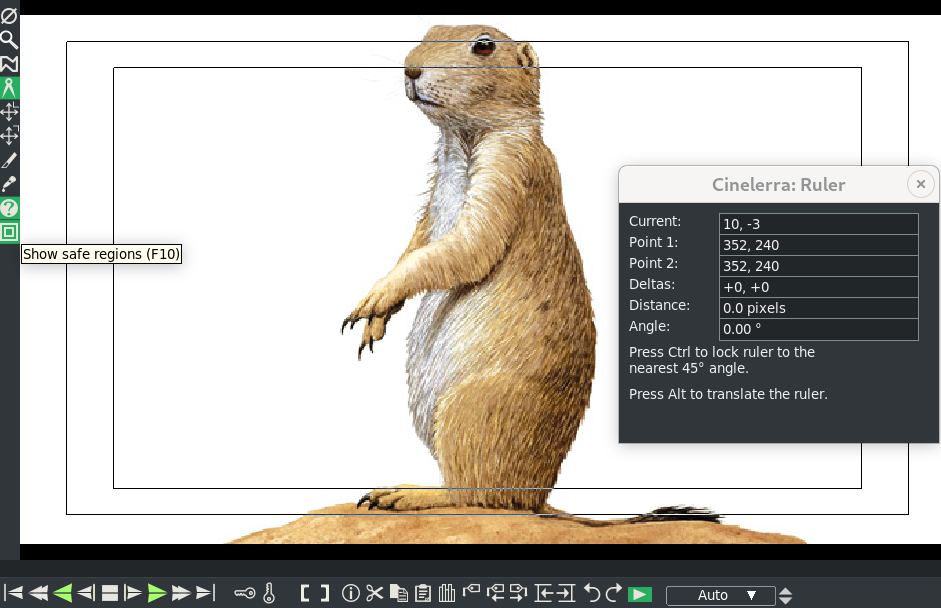
\includegraphics[width=0.9\linewidth]{safe_regions.png}
    \caption{Note the black outlines showing the safe regions. Also note the Ruler menu}
    \label{fig:safe_regions}
\end{figure}

    \item[Show safe regions]  draws 2 outlines to display the safe regions in the video as you
can see in Figure~\ref{fig:safe_regions}.
On some particular TVs/monitors/displays, the borders of the image are cut off and that
cut off section might not be as square as it appears in the compositor window. 
These are especially useful if the device for the output display is an older model TV\@.
The outside largest outline is the \textit{action safe overlay}; whereas the inside smallest
outline is the \textit{title safe overlay}.

Using the \textit{Show safe regions} has no affect on the rendered output.
The purpose of showing the borders is to make it easy to see where it might be cut off.  This
area outside the safe region can then be used as
a scratch or vertical blanking space.  Enabling the safe regions makes it really
easy to see these borders so that you can make sure 
titles are inside the inner outline and actions are inside the outer outline.

\end{description}

\subsection{Compositing}%
\label{sub:compositing}

Much of the editing in \CGG{} involves "compositing" which is the combining of visual
elements from different sources into single images.  This includes such things as 
speeding up and slowing down the video, changing the resolution, creating a split screen, and fading in and out.
Compositing operations are done on the timeline and in the Compositor window using various
operations and other compositing attributes that are available in the Resources window.
When \CGG{} is performing a compositing operation it plays back through the
compositing engine, but when not, it uses the fastest decoder that it has.

\subsection{The Temporary, Track and Output Sizes}%
\label{sub:track_and_output_sizes}

This section explains a few things which help to understand Compositing - especially with relation
to the camera, effects, and the projector.

\subsubsection*{The Temporary}%
\label{ssub:output_size}

\CGG{}'s compositing routines use a \textit{temporary} which is a single frame of video in
memory where graphics processing takes place. The size of the temporary and of the output in
the compositing pipeline are different and vary for any particular frame.  Effects are processed in
the temporary and as such are affected by the temporary size.  In the case of the camera, its
viewport is the temporary size. However, projectors are rendered to the output and so are affected
by the output size. When the temporary is smaller than the output, the temporary will have blank
borders around the region in the output.  When the temporary is larger than the output, it will be
cropped.

\subsubsection*{Track and Output size}%
\label{ssub:track_size}

The \textit{Track size} is used to define the temporary size with each track having a different size (viewports).
You can see or set the track size by RMB click on a track and then select \emph{Resize Track} to resize
the track to any size. Or select \emph{Match output size} to make the track the same size as the
output.  When a track is resized what it looks like on the compositor changes.  The relationship
between the track and the project's output size makes it possible to magnify or reduce the size of
a track in regards to the final output. This feature means you cancreate visual effects such as split
screens, zooms, and pans in the compositor.

The \textit{Output size} can be set in \texttt{File $\rightarrow$ New} when creating a new project,
or by using \texttt{Settings $\rightarrow$ Format}, or in the Resources window with RMB click on
a video asset and choosing \texttt{Match $\rightarrow$ Match project size}. When you \emph{Match project size}, you
are conforming the output to the asset. To change the size and aspect ratio of the output (Projector) we have to change the whole project, which will alter all the tracks in the timeline. Once you have set the output size in 1 of these 3 ways,
any newly created tracks will conform to the specified output size.  When rendering, the project's
output size is the final video track size where the temporary pipeline is rendered into.  

\subsection{Camera and Projector}%
\label{sub:camera_and_projector}

In the compositor window, \textit{Adjust camera automation} and \textit{Adjust projector automation}
are editing tools to control operation of the camera and projector.  In \CGG{}'s compositing
pipeline, the camera determines where in the source the \textit{temporary} is copied from while
the projector determines where in the output the \textit{temporary} is copied to
(figure~\ref{fig:temporary-01}). 

\begin{figure}[htpb]
    \centering
    \includegraphics[width=0.8\linewidth]{temporary-01.pdf}
    \caption{Compositing pipeline}
    \label{fig:temporary-01}
\end{figure}

In compositing, each frame can be changed using various options and plugins, such as
a color correction plugin (figure~\ref{fig:camera_and_projector}).  After the image has been
modified, the final image is projected to the compositor so that you now have a changed original.

\begin{figure}[htpb]
    \centering
    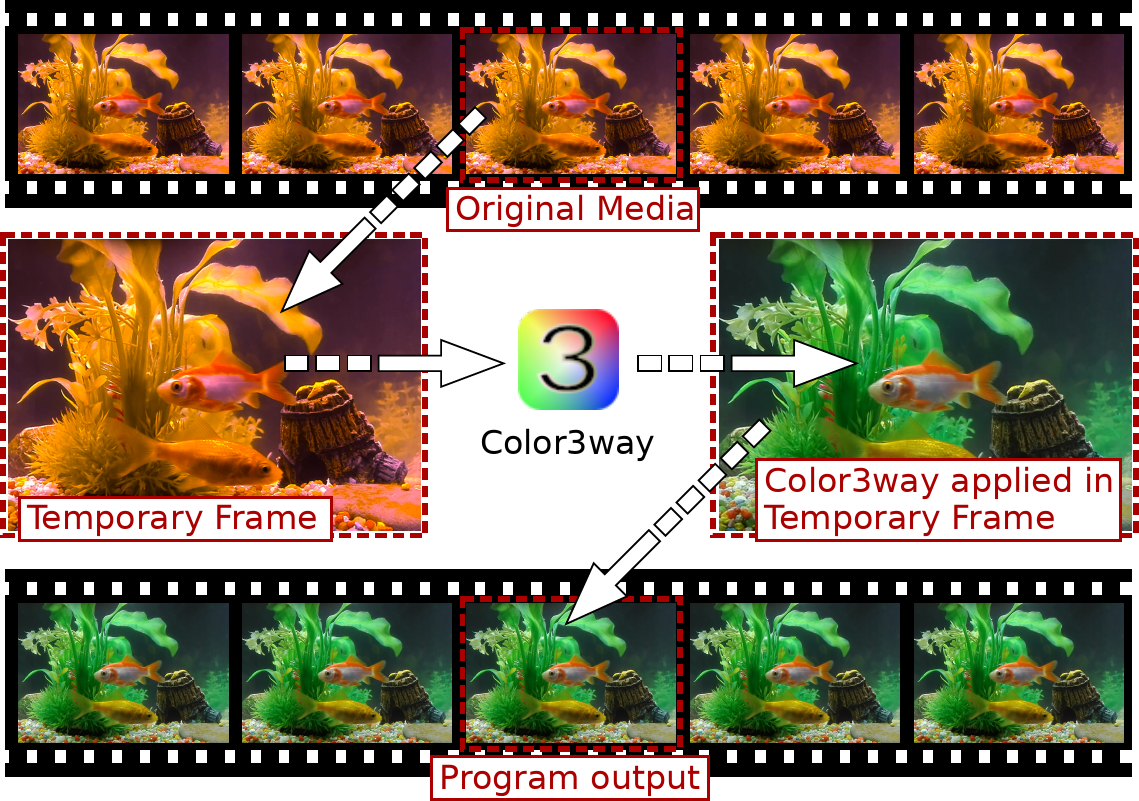
\includegraphics[width=0.8\linewidth]{camera_and_projector.pdf}
    \caption{Color3way on Temporary}
    \label{fig:camera_and_projector}
\end{figure}

When editing the camera and projector in the compositing window, the affected track will be the
first track that is armed.  If there are multiple video tracks, you can select one specific track
for editing with a LMB click on the \textit{Arm track} icon of the desired track. This is called
"solo" the track. To reverse this solo-ing, LMB click on the icon again. 

\subsubsection*{Projector Compositing}%
\label{ssub:projector_compositing}

The purpose of the \textit{projector} is to composite several sources from various tracks into one
output track.  The projector alignment frame is the same as the camera's viewport, except that it
shows where to put the contents of each temporary on the output canvas.  To get into projector
editing mode, click on the \textit{Adjust projector automation} icon in the Compositor toolbar. You
will then see red border lines surrounding the image and 2 diagonal lines criss-crossing in the 
middle, displayed in the video window.  The red outline indicates the size of the frame that will be
sent to the Output. You can easily drag the box with LMB, moving the frame in $x$ and $y$ directions.
When moving along the $z-axis$ (i.e.\ the zoom, with SHIFT+Drag) the box exactly follows the movement
and the size of the frame. After you position the video with the projector, you may next want to
\textit{Adjust camera automation}.

\subsubsection*{The Viewport}%
\label{ssub:viewport}

The \textit{viewport} is a window on the camera that frames the area of source video. The size of the current track is used for the initial size of the viewport. A smaller viewport, for example ($640\times480$), captures a smaller area; whereas a larger viewport of ($800\times600$) captures a larger area.  If the captured area is larger than the source video, the empty spaces will be automatically filled with blanks.  To change the size and aspect ratio of the viewport (Camera) of a single track, right-click on the track in the timeline and choose Resize Track. Here we can vary the height and base of the viewport in pixels or choose the multiplication coefficient for each side (Scale). With OK we will see the change in the Compositor window with the new dimensions reflected in the green box. We can have different size viewports for each video track on the timeline. To go back, reset the viewport to the original value. After the viewport is defined, the camera needs to be placed right above the area of interest in the source video. Operations to control the location of the camera are as follows:

\begin{enumerate}
    \item  In the compositor window you should see the selected track.
    \item  LMB click on the \textit{Adjust camera automation} to bring up the editing menu and the 
green and yellow colored outlines.
    \item  Use the LMB to drag the video over the display in the compositor window to the desired
placement.
\end{enumerate}

When you drag over the viewport in the compositor window, it looks like you are moving the camera
with the mouse.  The viewport moves in the same manner.

\subsubsection*{Camera Compositing}%
\label{ssub:camera_compositing}

Select the camera button to enable camera editing mode. 
In this mode, the guide box shows where the camera position is in relation to past and future camera positions but not where it is in relation to the source video. 
The green box is the Viewport; at the beginning it coincides with the size of the source frame. If we move the viewport by dragging it with LMB (moving it in $x/y$), the green box remains fixed to the original size but the frame is moved to the new position.  A yellow frame will appear along the edges of the frame to indicate the displacement with respect to the green box; this behavior differs from that seen for the Projector. Even if we act on the $z-axis$ (SHIFT + Drag, equivalent to the zoom), the frame narrows or widens, moving behind the yellow frame.

\subsubsection*{Camera and Projector Menu}%
\label{ssub:camera_and_projector_menu}

The camera and projector have shortcut operations that do not appear in the popup menu and are not represented in video overlays. 
These are accessed in the \emph{Show tool info} window.
Most operations in the Compositor window have a tool window which is enabled by activating the question mark icon (figure~\ref{fig:camera_tool}).

\begin{wrapfigure}[10]{O}{0.45\linewidth} 
	\vspace{1ex}
    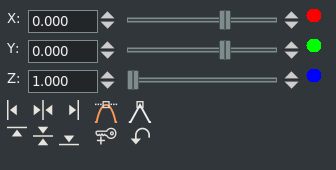
\includegraphics[width=1.0\linewidth]{camera_tool.png}
    \caption{Camera and Projector tool}
    \label{fig:camera_tool}
\end{wrapfigure}

In the case of the camera and projector, the tool window shows $x$, $y$, and $z$ coordinates. 
By either tumbling or entering text directly, the camera and projector can be precisely positioned.  
Justification types are also defined for easy access. 
A popular justification operation is upper left projection after image reduction. 
This is used when reducing the size of video with aspect ratio adjustment.  
In the last figure you see the choices for justification as the location of the line in the 6 boxes in the order of left, center horizontal, right, top, center vertical, and bottom.

The translation effect allows simultaneous aspect ratio conversion and reduction but is easier to use if the reduced video is put in the upper left of the \textit{temporary} instead of in the center. 
The track size is set to the original size of the video and the camera is centered. 
The output size is set to the reduced size of the video. 
Without any effects, this produces just the cropped center portion of the video in the output.

The translation effect is dropped onto the video track. The input dimensions of the translation effect are set to the original size and the output dimensions are set to the reduced size. 
To put the reduced video in the center subsection that the projector shows would require offsetting out $x$ and out $y$ by a complicated calculation. 
Instead, we leave out $x$ and out $y$ at 0 and use the projector's tool window. 
By selecting left justify and top justify, the projector displays the reduced image from the top left corner of the \textit{temporary} in the center of the output.

\subsubsection*{Reset to Default}%
\label{ssub:reset_default}

In the compositing window, there is a popup menu of options for the camera and projector. Right click over the video portion of the compositing window to bring up the menu:

\textit{Reset Camera}: causes the camera to return to the center position.
    	
\textit{Reset Projector}: causes the projector to return to the center.

\subsubsection*{Use Case: Interaction Between Camera And Projector \protect\footnote{Example provided by Sam. The relative video is located at: \url{https://streamable.com/iq08i}}}%
\label{ssub:use_case_interaction_camera_projector}

\begin{enumerate}
    \item Start by shrinking the projector to $z=0.500$ ($\frac{1}{4}$ of the original frame).
    \item The next step is to switch to the camera and note that the green box has assumed the size of the projector, i.e.\ the red box. The value of $z$ of the camera is always equal to $1.000$ (default) but the frame is $\frac{1}{4}$ of the original frame, i.e.\ it has the size of the projector that has $z=0.500$. This is the current viewport size.
    \item You enlarge the room bringing $z=2.000$. You can see that the dimensions of the viewport (green box) do not change, remaining the same as those of the projector. However, the frame has been enlarged and this variation is indicated by the enlargement of the yellow box. Let's remember that this follows the changes made with the camera tool.
    \item We can drag the room so that we can center the frame to our liking. The movement of the yellow box shows well the variation compared to the green box.
    \item Finally, if we want, we can switch to the projector tool to move the output frame to the position we want with respect to the size of the source. Of course, we can also work on the $z$, which in the example is at $z=0.500$, if we have decided to change the size of the output.
\end{enumerate}

\subsection{Masks}%
\label{sub:masks}

Masks can be used to accomplish various tasks but basically are used to select an area of the 
video to be displayed or hidden. 
They can be used in conjunction with another effect to isolate the effect to a certain region.
Another usage is where you slightly delay one video track copy and unmask an area where
the one copy has interference but the other copy does not.  Or use a mask when  color correction is
needed in one part of a frame but not another.  A mask can be applied to just a small section of
a color corrected track while a plain track shows through. 
Removal of boom microphones, license plates, people and airplanes via mask is a very common usage.

The order of the compositing pipeline affects how masks are done. Usually masks are operated on the
temporary, after the effects but before the projector. Because of the way this works, multiple
tracks can be bounced to a masked track and projected with the same mask.

The compositing pipeline graph has a masking stage (figure~\ref{fig:temporary-02}).

\begin{figure}[htpb]
    \centering
    \includegraphics[width=0.7\linewidth]{temporary-02.pdf}
    \caption{Compositing pipeline with mask}
    \label{fig:temporary-02}
\end{figure}

\subsubsection*{Compositing pipeline with masks}%
\label{ssub:compositing_pipeline_with_masks}

The Mask popup menu can be overwhelming upon first encounter.  However, if you follow the next
few steps you can create a single simple mask without having to understand every possible parameter.
\begin{enumerate}
    \item To define a mask, in the Compositor window click on the \textit{Edit mask} icon to get the popup Mask menu.  If the menu does not come up, click on the \textit{Show tool info}.
    \item  On the video, LMB click on the place where you want to start a mask.
    \item  Then LMB click on another spot of the image to create each new point of the mask. Once
you have at least 3 points, lines will be drawn between them, but you can just create as many
more points as you need and the lines will be redrawn to cover all points. When you 
create each point of the mask a straight line curve is expanded, altering the shape of the mask.
The mask position will always be in the same position on each image of the video unless you enable 
\textit{Generate keyframes while tweaking} on the Program window Transport and Buttons bar. Then when 
enabled you can move a mask over time.
     \item For a mask to be seen or not seen, there must be another video track under the track
that you are viewing in the compositor.  An easy way to see the masked area is to just add an empty track
below the target track and drag the \textit{Gradient} plugin to a highlighted area on that track.
     \item  You can move existing points to new locations by simply using the LMB at a point to
drag that point to a different location.
    \item  The mask can be translated as a single entity by Alt-dragging the mask.  For some desktop
window managers, such as \textit{UbuntuStudio 16.4} and \textit{Arch}, the Alt key is already in use
by the Operating System so you will have to use Alt+Ctrl instead.
    \item To create curved instead of straight lines between the points, use  Ctrl-drag on a
specific point. Using Ctrl-drag activates bezier handles (control points) to create these curves
between the points. For example, on a mask with just two points, you can create a romantic heart mask.     
\end{enumerate}

There are a lot more operations you can do using the Mask menu as shown in 
figure~\ref{fig:mask_window}.  Detailed description is provided here next.  Note that the Mask
window is separated into various sections to make it easier to locate the area of interest.

\begin{figure}[htpb]
    \centering
    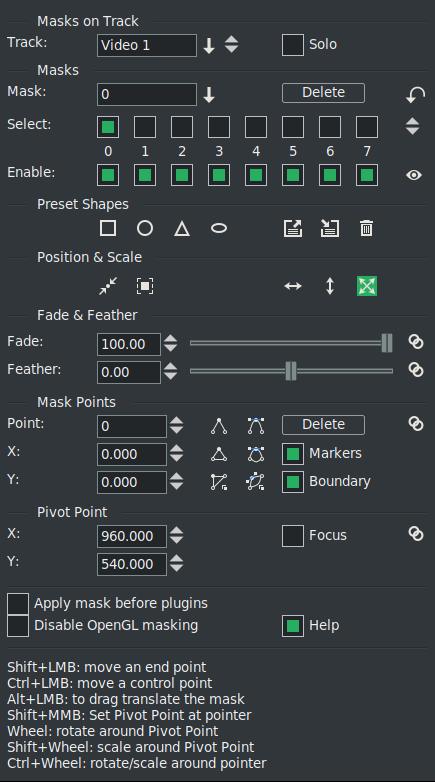
\includegraphics[width=0.5\linewidth]{mask_window.png}
    \caption{Mask options window}
    \label{fig:mask_window}
\end{figure}

\subsubsection*{Masks on Track section}%
\label{ssub:masks_track_section}

The \textit{Track}: textbox displays the different video tracks for your session which will be initially set to the first armed video track or will be left blank if there are no armed tracks.  A pulldown to the right of the box brings up the names of all of the video tracks allowing you to change to which track the masking applies.  You can also just use the tumbler to easily mouse up/down to get to the desired track. In the pulldown list, any track that has a red colored text name is disarmed so that you can not change it.  A track that contains masks has yellow colored text for easy identification.  Only when there are no masks on the track, do you have the default text color. This textbox is display only and you can not type into it.

The \textit{Solo} button in the Masks on Track section of the Mask window is very handy when working with masks on different tracks.  It displays just that track so that you see only the track you choose, as well as the tracks behind it to show the mask part.  The Solo button is just a convenience to prevent having to mouse over to the patchbay.

\subsubsection*{Masks section}%
\label{ssub:masks_section}

The \textit{Mask}: textbox will show you the mask numbers of $0-7$ or the 8 ascii character name that you have used to designate each mask number.  There is a pulldown on the right side to easily switch to another mask. 

The \textit{Delete} button is used to delete the mask number/name that is selected. The symbol to the right with tooltip of \textit{Delete all masks} can be used to delete all of the current video track masks.

The \textit{Select}: row of checkboxes is used to indicate which mask is currently displayed for that video track in the Compositor.  Numbers that are colored yellow are active masks for that track.  A tumbler to the right allows for quickly changing the mask number displayed.

The \textit{Enable} row of masks makes it so you can enable all or none of the masks, making it possible to look at no masks or at one mask without interference from the other masks. The symbol that looks like an \texttt{eye} can be used to easily check all or none as the tooltip \textit{Show/Hide mask states}.

\subsubsection*{Preset Shapes section}%
\label{ssub:preset_shape_section}

There are 4 shapes that are automatically available for usage as masks – square, circle, triangle, and oval.  In addition, the next 3 symbols in this section are for the purpose of loading, saving, and deleting your own customized shapes.  The first symbol, \textit{Load} preset, will bring up a list of your previously saved presets.  Clicking on \textit{Save} preset brings up a popup window allowing you to provide a name used to identify the preset you want to save, along with a pulldown to see the names of your other saved presets.   Clicking on \textit{Delete} preset also brings up a textbox with a pulldown to choose which one to delete.  There is a file, called \texttt{mask\_rc}, in \texttt{\$HOME/.bcast5} that records your custom masks.  

When you click \textit{Load} preset, keep in mind that it will write the mask number that you have selected so if you already have a mask at that location, it will write over it – just \textit{Undo mask} under the main window Edit pulldown (shortcut `z') to revert to the previous if you made this mistake.

\subsubsection*{Position \& Scale section}%
\label{ssub:position_scale_section}

\textit{Center} mask button allows for quickly centering a mask on the video track. 
\textit{Normalize} mask button makes it easy to normalize the size of the mask based on the scale of the video. 
The next 3 symbols concern the direction to \textit{drag translate} a mask using the \texttt{Alt+LMB} thus making it easy to preserve the current $X$ or $Y$ value when desirable.  For some desktop window managers,
such as \textit{UbuntuStudio 16.4} and \textit{Arch}, the Alt key is already in use by the Operating System
so you will have to use Alt+Ctrl instead.

\texttt{xlate/scale x}	- drag translate constrained in the $X$ direction

\texttt{xlate/scale y}	- drag translate constrained in the $Y$ direction

\texttt{xlate/scale x/y}	- drag translate in both directions; this is the default and after using the other 2 options, you should reset to this to avoid future confusion while dragging.

\subsubsection*{Fade \& Feather section}%
\label{ssub:fade_feather_section}

The \texttt{Fade}: textbox is used to type in a fade value; the tumbler to the right of the textbox allows you to increase or decrease that number; and the slider bar makes it quick to adjust the fade value.  The fader goes from $-100$ on the left to $+100$ on the right for negative to positive.  Default value is $+100$. The fade slider includes a sticky point at 0 so that it is easy to get to 0 without going too far or not quite far enough -- that way you don’t have to keep jiggling to get there. 

In addition there is a \textit{Gang fader} symbol to allow for having all of the masks fade in unison. The symbol is surrounded by a green colored background \protect\footnote{green is used in the default Cakewalk theme, but the background color will be different in other themes} when it is in effect.  If you have multiple masks with different modes, a decision had to be made on what value to use -- it uses the maximum transparency value of the background to determine the operations results.  To understand how this works, here is a summary:

Note1: The area outside the mask is referred to as the background.

Note2: The operational result is based on the maximum transparency value of that background.

\paragraph{Case 1, Positive Fade:} When the fade for all of the masks is positive, affecting the area inside of the mask, all of the
background colors are at a transparency value of zero. So the largest transparency value is 0,and all masks are drawn with opaque backgrounds, depicted as one would expect.

\paragraph{Case 2, Negative Fade:} When the program computes the background color for any number of masks that includes negative
mask(s), it uses the largest transparency number as the determining factor for the background. Only 1 of the masks can be largest, and wins for the background transparency result.

\vspace{3ex}\textit{Feather}: works in a similar manner to a \textit{gradient Fade} aligned on the mask boundary but is a logical function instead of a mathematical function so will be faster.  The \textit{Gang feather} symbol also works in a similar fashion and is surrounded by a gold colored background when it is in effect.

\subsubsection*{Mask Points section}%
\label{ssub:masks_points_section}

This section is used to change to a different mask number and manipulate the masks you have created.

The \textit{Point}: textbox provides the ability to change which point number for the current mask that you want to work on.  It has a tumbler to allow for quickly switching the point number.  The \textit{X:} and \textit{Y:} boxes below reflect the current values and allow for modifying the $X/Y$ coordinates and these too have tumblers. The \textit{Delete} button will allow for deleting the selected point number.

The next 6 symbols in 2 columns represent \textit{Smooth} and \textit{Linear} buttons.  Smooth buttons use an algorithm based on the previous point and the next point to create a curved line. The smoothing operation takes three points, A, B, C, and arranges the slope at B to be AC as it moves to the next point for that mask.

\textit{smooth point}	$\rightarrow$ smooth a single point.

\textit{smooth curve}	$\rightarrow$ smooth all points on a mask edge curve.

\textit{smooth all} 	$\rightarrow$ smooth all active masks.

Linear buttons of \textit{linear point}, \textit{linear curve}, and \textit{linear all}, perform the inverse of the smooth functions.
The control point vectors on the bezier endpoints are set to zero magnitude.

In addition there is a \textit{Markers} and a \textit{Boundary} checkbox which come in handy to turn off the display of the points and the outline of the mask.  Turning off \textit{Markers} is very useful when you have a lot of control points that clutter the display and make it more difficult to see the actual mask.  A helpful feature is available by disabling \textit{Markers} and enabling \textit{Boundary} which results in all masks being displayed in the viewer; for example you can then see mask 0, mask 1 \dots at the same time.

A \textit{gang} symbol on the right hand side of this section, tooltip of \textit{Gang points}, is another useful feature that makes it easy to drag a mask to an exact coordinate using the \textit{X} or \textit{Y} textbox for numerical input or the associated tumblers.  This works like the \texttt{Alt+LMB drag} translate but provides the ability to be precise.

\subsubsection*{Pivot Point section}%
\label{ssub:pivot_point_section}

The \textit{X:} and \textit{Y:} coordinates mark the value of the current \textit{Pivot Point} used for rotation, scaling, and translation.  You can either directly key in numerical values or use the tumblers to change the values as long as the \textit{Focus} checkbox is checked.

The \textit{Focus} checkbox is used in case you want to set a different point in the Compositor for pivoting instead.  And the \textit{Gang} symbol for rotate/scale/translate means that these operations will be performed on all points of the enabled masks.  The gang symbol is surrounded by a gold colored background when it is in effect.  When performing a rotate operation on a mask with the mouse wheel, \textit{acceleration} is in effect -- this means the faster you wheel, the more space is covered so that you do not have to wheel dozens of time to make a full rotation.  Then when you wheel around slower, you can fine tune the result.
Note that in order to be able to rotate/scale around pointer, the Focus checkbox must be unchecked.

\subsubsection*{Other sections}%
\label{ssub:other_sections}

Finally there are the \textit{Apply masks before plugins} and \textit{Disable OpenGL masking} self-explanatory checkboxes.

Note: Not all OpenGL software can support the current masking methods.  If your opengl implementation does not support Shader Version 4.3 or has trouble with this (it is relatively new to opengl at the time this was implemented), then this checkbox will allow you to use the software masking to avoid any potential issues.  Normally, OpenGL is probed for the shader version and will automatically use the software implementation if required.

The \textit{Help} checkbox can be enabled in order to see a list of the keys used to perform various operations.  If you use Masking infrequently, these are a valuable reminder to which key combinations to use.  Currently they are as follows:

\vspace{2ex}
\begin{tabular}{ll}
    \hline			
    Shift+LMB & move an end point \\
    Ctrl+LMB & move a control point \\
    Alt+LMB & to drag translate the mask \\
    Shift+MMB & set Pivot Point at pointer \\
    Wheel & rotate around Pivot Point \\
    Shift+Wheel & scale around Pivot Point \\
    Ctrl+Wheel & rotate/scale around pointer \\
    \hline  
\end{tabular}

\subsubsection*{Key Alternatives}%
\label{ssub:key_alternatives}

\vspace{2ex} Note: For some desktop window managers, certain keys may already be in use by the operating system, so you will either have to redefine them in your desktop or use different key combinations.  For example, at least some desktops used with \textit{UbuntuStudio 16.04} and \textit{Arch} field the \texttt{Alt} key, thus requiring alternative key combinations to be needed.  Below are some of these alternatives.

\vspace{2ex}
\begin{tabular}{lp{11cm}}
    \hline			
    LMB & move/create an end point (to move the end point the pointer must be above the point) \\
    Shift+LMB & move an end point (the pointer may be near the point, not above it) \\
    Ctrl+LMB & move/create a control point \\
    Alt+Ctrl+LMB & to drag translate the mask \\
    Shift+Key Delete & to delete the mask \\
    Shift+MMB & Set Pivot Point at pointer \\
    Alt+Wheel & zoom in/out the screen (also available in Ubuntu16 but does not exist in all distros) \\
    \hline  
\end{tabular}

\vspace{2ex}
Focus checkbox = unchecked:

\vspace{2ex}
\begin{tabular}{ll}
    \hline			
    Wheel & rotate around Pivot Point \\
    Shift+Wheel & scale around Pivot Point \\
    Ctrl+Wheel & rotate around pointer \\
    Ctrl+Shift+Wheel & scale around pointer \\
    
    \hline  
\end{tabular}

\vspace{2ex}
Focus checkbox = checked:

\vspace{2ex}
\begin{tabular}{ll}
    \hline			
    Wheel & rotate around Pivot Point (“Custom focus point”) \\
    Shift+Wheel & scale around Pivot Point (“Custom focus point”) \\       
    \hline  
\end{tabular}

\vspace{2ex}

\subsection{Cropping}%
\label{sub:cropping}

Cropping is used to reduce the visible picture area by changing the output dimensions, width and
height in pixels, and the $X, Y$ values. An example of cropping and the crop menu is seen in
figure~\ref{fig:cropped_area}.
The easiest way to use cropping is to click with the LMB 
at the spot to begin cropping and while holding down the LMB, drag the mouse. This creates a rectangular
cropping area.  To change the size/location of that area, click on any of the 4 corner points
with the LMB and drag.  While dragging, you will see 
the X1, Y1 coordinates and W for width, H for height, in the Crop tool popup menu
automatically change numerical value to reflect the current position. For precise locations, you
can keyin exact values into those textboxes instead of using the mouse.
Once you have the crop area defined as you want it, then click on the \textit{Apply} button to have
the actual cropping take affect.

There are 3 choices of crop methods to choose in the menu pulldown on the bottom right side.
\begin{enumerate}
     \item Reformat - Reformat Session crops and changes the Format for the entire session. 
Because the Format is changed, this is applied to all tracks in the project.
The part of the image outside the rectangle will be cut off and the projector will make the video fit.
The  \texttt{Settings $\rightarrow$ Format} window will show the new project Width and Height values and
the projector tool window will show the new $X, Y$ values. Track size remains unchanged.
You can undo the cropping by entering the original project dimensions in the
\texttt{Settings $\rightarrow$ Format} window for the Width and Height.  You will also have to use the Projector
tool in the Compositor toolbar to \textit{Ajdust projector automation} by clicking on the Reset icon.
     \item Resize - Resize Projector; to undo this, enable \textit{Adjust projector automation} 
and do a Reset.
     \item Shrink - Resize Projector and Camera; to undo this, enable each of the \textit{Adjust
projector and camera automation} tools, one at a time, and do a Reset in the menus.
\end{enumerate}
An important note here is that the original aspect ratio will be maintained so if your frame is
rectangular (as many are) and you "crop" by surrounding the region of interest with a square,
the cropped area will be more than you marked in order to keep the aspect rectangular shape.
The Resize and Shrink options are applicable to all video tracks except the disarmed ones. 
This is in contrast to the Reformat option, as mentioned previously, which applies to all tracks even if disarmed because it changes the Format for the session.
One last note of interest, this cropping is keyframable.

\begin{figure}[htpb]
    \centering
    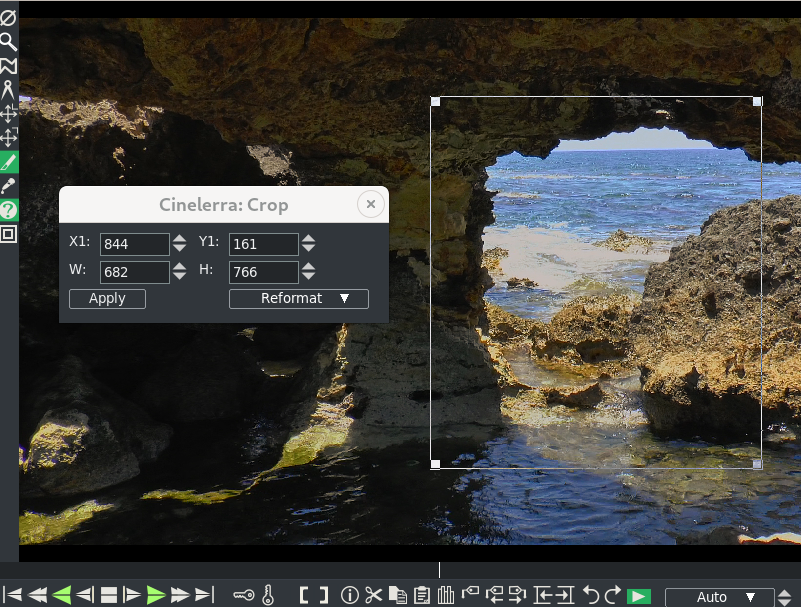
\includegraphics[width=0.9\linewidth]{cropped_area.png}
    \caption{Crop menu and outlined crop rectangle on the right side}
    \label{fig:cropped_area}
\end{figure}

An easy to follow step by step usage of the cropping tool is outlined next.
\begin{itemize}
    \item Enable the crop tool in the compositor window to display the Crop popup menu.
    \item Click-drag in the video to define the crop area which draws a rectangle on the video.
    \item Click-drag in the video to start a different rectangle instead.
    \item Click-drag on a corner of the rectangle to reposition that corner.
    \item Alt-click in crop rectangle to translate the rectangle to a different position without resizing.
    \item The crop popup menu allows text entry of the top left coordinates ($X1,Y1$) and width and
height ($W, H$) that define the crop rectangle. 
    \item Choose one of the 3 options of Reformat, Resize, or Shrink.
    \item When you have the rectangle where you want it,
click on the \emph{Apply} button in the menu to actually perform the crop operation.
\end{itemize}
 

\section{Viewer Window}%
\label{sec:viewer_window}

The Viewer window (figure~\ref{fig:viewer_window}) is convenient for previewing your media and 
clips. It can also be used for editing with cuts and then paste operations into the timeline or
to create a clip.  There are transport buttons to use in the same manner as in the Program
and Compositor windows or you can quickly move through the media by dragging with the LMB in
the timebar above the transport buttons.  

\begin{figure}[htpb]
    \centering
    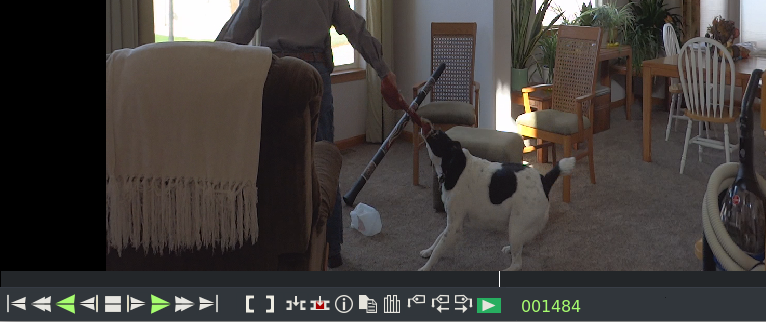
\includegraphics[width=0.99\linewidth]{viewer_window.png}
    \caption{Viewer Window - the red arrow "Play" button is left of the Videoscope button}
    \label{fig:viewer_window}
\end{figure}

In order to view media in the window, you have to load it as follows:

\begin{enumerate}
    \item  In the Resources window, highlight the Media folder or the Clip folder.
    \item  Drag a file from the folder to the Viewer.
    \item  \textbf{Or} double LMB click on a media asset.
    \item  \textbf{Or} highlight an asset, RMB to bring up choices, and click on \textit{View} or
\textit{View in new window}.
\end{enumerate}

Note that you can have multiple Viewer windows open with different or even the same media asset.
After the media is loaded you can use the transport buttons to play, rewind, stop, and so on, or
for fast previewing drag with the LMB anywhere on the timebar slider.  There is also the Videoscope
button which is to used to enable the scopes window without having to apply the filter to the tracks/edits.
A few more options available in the Viewer window can be accessed with a RMB click on the display.
These functions are listed next.

\begin{enumerate}
    \item  Switch to a fullscreen display by choosing \textit{Fullscreen}.  To switch back, click
with the RMB on the display again and choose \textit{Windowed}.
    \item  Change the display size by choosing the \textit{Zoom} function to select a zoom level of
25\%, 33\%, \ldots 300\%, or 400\% of the original media size.
    \item  To remove the current media from being displayed, choose \textit{Close source}.
\end{enumerate}

The Viewer uses the project's output size format settings to display the media instead of the
original asset's format. Operations performed in the Viewer affect a temporary EDL or a clip rather
than the timeline.  By default, the Viewer window is automatically available but if it gets
accidentally closed you can open it again by using the pulldown \texttt{Window $\rightarrow$ Show
Viewer} to bring it back up.  More details for editing in the Viewer window with the Two Screen
Editing method is explained in~\ref{sec:two_screen_editing}.


\begin{figure}[htpb]
    \centering
    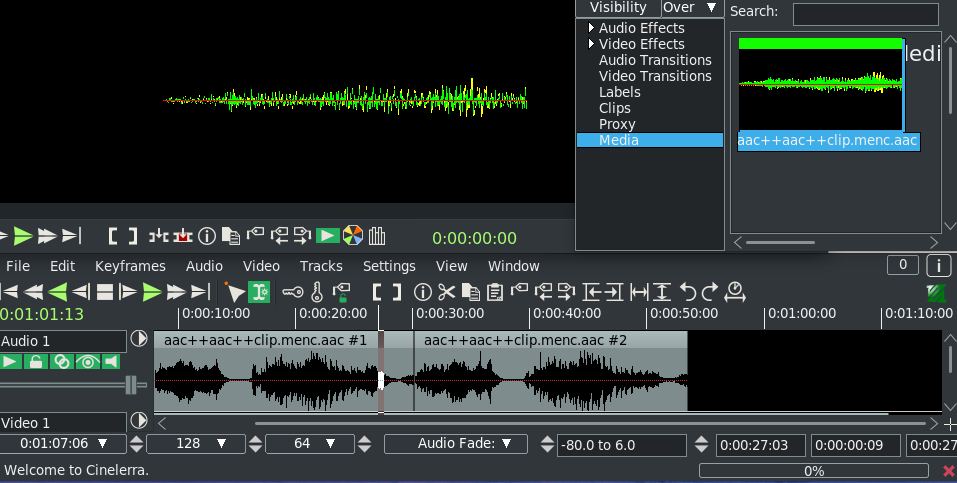
\includegraphics[width=1.0\linewidth]{viewer_audio.png}
    \caption{Viewer window at the top displaying same 5 seconds as seen in the Resources window thumbnail. At the bottom of the screen is the audio loaded on the timeline.}
    \label{fig:vieweraudio}
\end{figure}

You can also use the Viewer to listen to media that consists only of Audio.  This is a quick way
to listen to the audio to see if it is what you would like to add to a timeline audio track for
your project.  To do this, you simply drag the audio file from the Resources window in the same
manner as a video file. The viewer was designed to "view" images rather than play audio so in order
to make it obvious that audio media is loaded to the viewer, a waveform is displayed that is the
same waveform as shown in the Resources window thumbnail when in the \textit{Display Icons} mode.
This waveform only represents the first 5 seconds of the media and will not change or move while
playing in the Viewer window.  But you can play the entire piece of media in the window
and as you do so, you see the play cursor line move along and the timestamp reflect the actual
position. You can also create clips. The entire waveform can only be seen on an actual audio track
on the timeline. An example of what this looks like is shown in figure~\ref{fig:vieweraudio}.

\section{Options in both the Compositor and Viewer Windows}%
\label{sec:options_in_both_the_compositor_and_viewer_windows}

The next sections describe capabilities that are available in both the Compositor and Viewer windows.

\subsection{Click to Play in Viewer and Compositor}%
\label{sub:click_to_play_in_viewer_and_compositor}

In both the Viewer and Compositor windows, there is an arrow on the right hand side of the other
buttons in the edit panel as shown in figure~\ref{fig:viewer_window}.  The "play" button can be
toggled on/off via this arrow, which has a tooltip of \textit{Click to play}.  When enabled
the arrow is white surrounded by green and when disabled the arrow is red.\protect\footnote{the color and the look will be different for themes other than the default theme of Cakewalk}
The purpose of enabling this capability is to make it really easy to play the media in the window
by just using the left mouse button to start or stop the play.  The entire main canvas surface
becomes a big play button!  Although the default is initially off, a good reason to enable this,
at least temporarily, is so that you can quickly review your video before a render.
 
\begin{description}
    \item[left click]  forward play or stop forward play if already playing
    \item[middle wheel]  single frame forward or back
    \item[middle click]  reverse play or stop reverse play if already playing. 
        Note that some 3 button mice do not accommodate a middle click for reverse but you can find out by testing from a terminal window with the command \texttt{xev}.
\end{description}

\subsection{Timebar + Preview Region Usage in the Compositor and Viewer}%
\label{sub:timebar_preview_region_usage_in_the_compositor_and_viewer}

The Viewer and Compositor each have a timebar control area with an indicator line below the video
output. The \textit{timebar} shows the whole time covered by the program. When a video asset
is loaded in the main window and you move in the compositor, the insertion pointer in the main
window will reflect those movements.  However, this is not the case with the viewer.  In the viewer
only that specific media is shown and there is no corresponding movement on the timeline.

Both the Compositor and Viewer support labels and in/out pointer which are displayed in the timebar.
And as with the movements, when you use the labels or in/out pointer in the compositor timebar,
the result will also be reflected in the main window timebar.  Along with that, of course, when
you move to a label or in/out pointer in the compositor, the insertion point in the program window
will go to that position.

The timebar in the compositor and the viewer can be used to define a region known as the \textit{preview region}.  
This preview region is the region of the timeline which the slider affects.  
By using a preview region inside the entire program and using the slider inside the preview region you can very precisely and relatively quickly seek in the compositor and viewer.  
The preview region can be especially handy when you have large pieces of media by previewing one section, then move to the next section.  

The active preview region is the zone between the edge bars.  
The full range of the window slider pointer action is down-scaled to the active preview region.   
To use this, set the preview active region as a media time region of interest.  
Now addressing the timebar with the mouse only operates as if the timebar is zoomed to the scale of the active preview zone.  
This has the effect of magnifying the interesting media in terms of the mouse pointer addressing, for fine-tuning.

\begin{figure}[htpb]
    \centering
    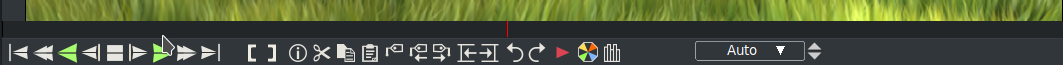
\includegraphics[width=1.0\linewidth]{timebar1.png}
    \caption{The arrow above the green colored “play forward” transport button is on the timebar.}
    \label{fig:timebar1}
\end{figure}

To create and use a preview region, hold down the right mouse button inside the timebar on either end of the timebar close to the edge until you see the resize pointer.  
While continuously holding the right mouse button down, drag the arrow away from the end towards the middle of the timebar until you have the desired area outlined.  
The slider will be a dark red color while the selected preview region will remain the same initial black color.  
There are either a left or right resize pointer and you can click and drag in either direction to expand or shrink the region.

\begin{figure}[htpb]
    \centering
    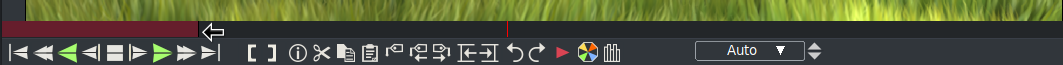
\includegraphics[width=1.0\linewidth]{timebar2.png}
    \caption{A left-facing arrow on the right side of the reddish slider bar is used to drag the bar.}
    \label{fig:timebar2}
\end{figure}

\begin{figure}[htpb]
    \centering
    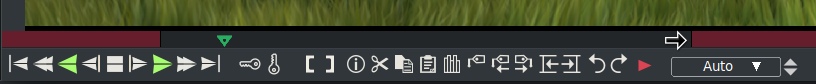
\includegraphics[width=1.0\linewidth]{timebar3.png}
    \caption{Here you can see the right-facing arrow used to drag the other end of the slider bar.  
        The black area between is the actual preview area.}
    \label{fig:timebar3}
\end{figure}

You can slide the preview zone left or right by holding the right mouse button over the preview zone where you will see a fat double headed arrow.  
The selected area will move left or right as you drag and still retains the same size.

\begin{figure}[htpb]
    \centering
    
\includegraphics[width=1.0\linewidth]{timebar4.png}
    \caption{Note the double-headed fat arrow in the preview area used  to move the selection over.}
    \label{fig:timebar4}
\end{figure}

Settings:

\begin{enumerate}
    \item  If no preview region is set, increasing the length of the media on the timeline by inserting media or
        appending, has no effect on the non-selected preview region.  That is, you will not see the blue slider
        suddenly mysteriously appear.
    \item  If the preview region is set, when you replace the current project or file,  the preview region is
        automatically disabled.
    \item  If the preview region is set, when you append data or change the size of the current project, the
        preview region may appear to either move, shrink, or grow depending on the new length of the
        media on the timeline.  
    \item  To disable the preview region, you will have to drag both the right and the left blue slider bars
        completely to their corresponding end so that there is no longer any visible red slider.
\end{enumerate}

A good method for taking advantage of the preview region is described here.  
On the main track canvas, scroll to the beginning of the area of interest.  
When you do that, you will see in the compositor the red indicator line of that location.  
Now in the compositor window, right mouse drag from the left side of the edge of the timebar to create the dark red slider bar line up to the red indicator.  
Back in the main track canvas, move to the location of the area you want to end looking and again you will see the red indicator line in the compositor.  
Use the right mouse drag from the right to stop at that end point.  Using this method is often easier than continuous usage of the single frame move which can be tedious.

One last interesting item of note -- sometimes you may wish to see just a little more that is outside the preview region and you can do so!  You can actually move outside the compositor or viewer window space and view more, at least until you hit the end of the monitor space.

\section{Resources Window}%
\label{sec:resources_window}

Effects, transitions, labels, clips, proxies, user bins, and media assets are accessed here. 
Most of the resources are inserted into the project by dragging them out of the resource window. 
Management of resource allocation is also performed here.

\begin{figure}[htpb]
    \centering
    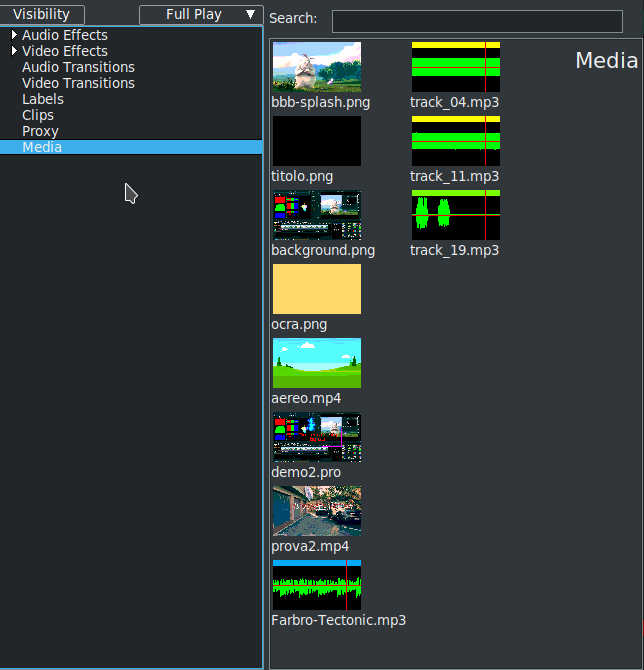
\includegraphics[width=0.8\linewidth]{resource_window.png}
    \caption{Folders are in the first column with contents of that folder on the right hand side}
    \label{fig:resource_window}
\end{figure}

The resources window is divided into two areas (figure~\ref{fig:resource_window}. 
One area lists folders and another area lists the folder contents. 
Going into the folder list and clicking on a folder updates the contents area with the contents of that folder. 
The folders can be displayed as icons or text. 
There are several variations for displaying the contents; select \emph{Display text}, \emph{Display icons}, \emph{Display icons packed}, \emph{Display icons list} as types of display for the assets or plugins. 
Use the letter “\texttt{V}” to easily scroll through the choices and see which you prefer.  
You can also get to these options from the menu by a right mouse click in the window.

A \emph{Search} option is available for any of the folders in the Resources window (and when using \textit{Attach effect} on the main track canvas for the Plugins).  
As you type in characters a match is made with that substring.  
Names that do not match are filtered out making it a lot easier to find the item you are looking for.  
The characters can be any where within the phrase and it does not matter if upper or lower case. 

Other options you will see if you \textit{right mouse click in the folder} which brings up the menu are described next.  

\begin{description}
    \item[ Load files ]  for convenience to load files same as from the main window so you do not have to move the mouse so far in case you have multiple monitors.
    \item[Display text/icons]  as described previously for format variations preference.
    \item[Select]  options are All, Used, Unused, and None.  This gives you the capability to have a set of the
        contents highlighted for ease of use so you can see what is or is not loaded, or unset the highlight.
    \item[Sort items]  to sort the contents of the folder alphabetically.  Especially helpful if you accidentally did a 
        drag and changed your mind or dropped suddenly so that the assets no longer look nicely aligned.
    \item[Copy/Paste file list]  use to easily copy a set of files or paste a set of files between \CGG{} and other programs or operating system windows.
    \item[Snapshot/Grabshot]  use to take a quick snapshot or to grab a specific area on the screen.  These functions are described in detail in section \ref{sub:snapshot_grabshot}).
\end{description}

Using the right mouse click to bring up a menu in the folder area, you can also switch from Display text to Display icons, Sort items and create, delete and manipulate user defined folders/bins. Select Folder to create a user Folder or modify an existing folder.

If you \textit{right mouse click on a highlighted/selected resource}, several options are available depending on whether the resource is an effect or transition or a piece of media.  
You can highlight several for some options so that it is applicable to all of them, such as Info.  
Those listed immediately below are the available choices for media assets.


\begin{description}
    \item[Info]  provided basic Asset information; details are described later in this section.
    \item[Display text/icons]  same as mentioned previously.
    \item[Sort]  same as mentioned previously.
    \item[Rebuild index] if you switch from/to using ffmpeg/native for media loading, you should rebuild
        indexes.  Or if you get hangs on media or strange looking tracks, you might want to rebuild indexes.
    \item[View]  use this option to bring up the media in the Viewer window.
    \item[View in new window]  in order to not overwrite your current viewer window, you can open any
        number of viewer windows to simultaneously view multiple media.
    \item[Open mixers]  when you record with multiple cameras setup, you can work with them most easily
        using the mixer mode.  This is described in detail
    \item[Paste]  
    \item[Match]  if you need to change your media parameters you can choose from the following: Match frame
        rate, Match project size, Match all 
    \item[Remove]  use to Remove the asset from the project or with caution, to Remove from disk permanently.
\end{description}

In the case of Effects or Transitions, a right mouse click on a highlighted selection leads to an \emph{Info} button which gives a short 1 line description of what the effect/transition can be used for.
For Labels, choices are \emph{Edit}, \emph{Label}, and \emph{Go to}.
For Clips, \emph{Nest} and \emph{UnNest} as described elsewhere are available.

\subsection{Info Asset Details}%
\label{sub:info_asset_details}

The asset \emph{Info} window also can be used to display detailed information about the selected/highlighted media file -- available for any loaded media of type mpeg or ffmpeg.  
This is extremely helpful in determining what type of media it is, size, resolution, format, and type/number of audio streams.  It is especially useful for multiple program streams.  You can have the info window popped on several of your assets simultaneously.

\textit{Asset's interlacing}  is the type of interlacing the asset has: If the file is (H)DV type, recognition and configuration is done automatically. All other media types will be set unknown. So we have to manually set the interlacing \protect\footnote{From Igor ubuntu's mail}.

Figure~\ref{fig:info_asset_details} shows the \textit{Detail} box to click on the left side and a simple, typical output in the Asset Detail window on the right side.  Also, note the highlighted media in the Resources window.

\begin{figure}[htpb]
    \centering
    \includegraphics[width=0.99\linewidth]{info_asset_details.png}
    \caption{The “Detail” box}
    \label{fig:info_asset_details}
\end{figure}

\subsection{User Folders/Bins}%
\label{sub:user_folders_bins}

Creating folders that are more specific to a particular project is helpful in better organizing your work.  
This can be done by utilizing the files already loaded to the \textit{master} Media or Clips folders in the Resources window.  The general rule is you can only drag clips to a ClipUserBin and you can only drag media to a MediaUserBin.

Below are steps illustrating an easy way to set up a folder.

%TODO Below part need to be rewriten
\begin{enumerate}
    \item In the Resources window (figure~\ref{fig:folder_resources}), in the location of the Video/Audio effects and Media folders, bring up the \textit{Folder}$\dots$ popup by clicking the right mouse button.  
        Highlight, then click \textit{New Media or Clips}.
        \begin{figure}[htpb]
            \begin{minipage}{.6\linewidth}
                \centering
                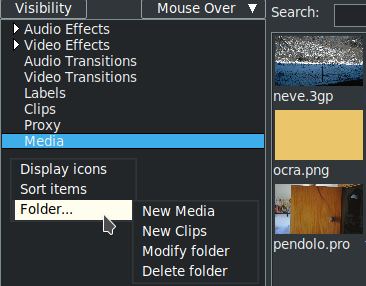
\includegraphics[width=0.9\linewidth]{folder_resources.png}
                \caption{Highlight, then click “New Media or Clips”.
                    “Modify folder” can be used to   change the name of a folder.
                    “Delete folder” in the popup can be used to delete a folder.
                }
                \label{fig:folder_resources}
            \end{minipage}
            \hfill
            \begin{minipage}{.37\linewidth}
                \centering
                \vspace{18ex}

                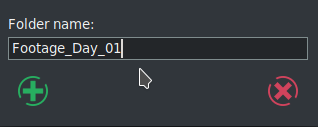
\includegraphics[width=0.9\linewidth]{folder_new.png}
                \caption{Type in your folder name in the textbox.  Click OK.}
                \label{fig:folder_new}
            \end{minipage}
        \end{figure}
    \item  In the \textit{New folder} popup as shown below (figure~\ref{fig:folder_new}), type in your folder name in the textbox.  Click OK.
     \begin{figure}[htbp]    
     	\centering
     	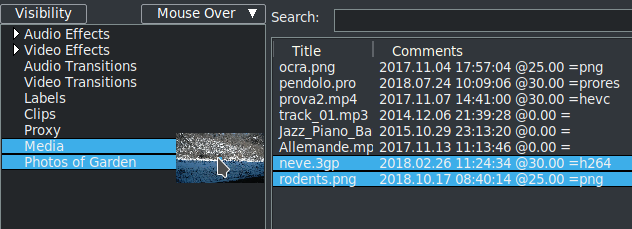
\includegraphics[width=0.9\linewidth]{folder_master.png}
     	\caption{The “master” Media folder}
     	\label{fig:folder_master}
     \end{figure}     
    \item  Select the \textit{master} Media folder to see which files are currently loaded, figure~\ref{fig:folder_master}.  
        Highlight the files there that you want to copy to your new folder (named Photos of Garden).  
        Drag the files to the left and when you see the Photos of Garden folder become highlighted, then drop there.  
        You can drag and drop any of the media from the \textit{master} Media at any time.  
        It flashes when the drop is successful.
\end{enumerate}

Adding the Shift key before the actual drop, will allow for relative path filenames instead of full path.
But you might want to include or eliminate some of the media that exists in one of the folders that you have set up already.  
In this case you will want to click on the \textit{Modify folder} in the popup.  
When you bring up the Modify folder window, if you already have files in that folder, you will see filters that were generated automatically when you did a Drag and Drop.


\begin{figure}[htpb]
    \centering
    %\includegraphics[width=0.8\linewidth]{name.ext}
    \begin{tikzpicture}[scale=1, transform shape]
        \node (img1) [yshift=0cm, xshift=0cm, rotate=0] {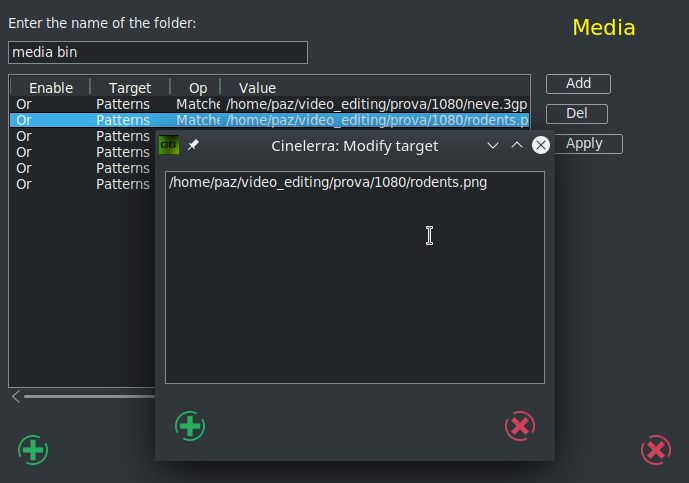
\includegraphics[width=0.7\linewidth]{folder_modify.png}};
        \node [yshift=-20mm, xshift=-1cm,anchor=east] at (img1.north west) (Arrow1) {\parbox{8em}{Here is the filter that was generated with the original drop }};
        \node [yshift=-65mm, xshift=0cm,anchor=east] at (img1.north west) (Arrow2) {\parbox{10em}{When you click on the Value portion of that filter, the entire set of files that are covered by the filter rules pops up.   Now you can highlight a target filename that you would like to remove, and just erase that line and check the green checkmark for OK.}};
        \draw [->, line width=1mm] (Arrow1) edge  ([yshift=-20mm] img1.north west);
        \end{tikzpicture}
    
    \caption{Modify target}
    \label{fig:modify-target}
\end{figure}

To delete the entire set of files listed on the filter rule, highlight the rule line and hit the \textit{Del} button.  
To add a new filter rule, click on the \textit{Add} button which will automatically add a default line after any current lines.  
The default line will be a line that matches everything in the \textit{master} Media folder which is \textit{Or  Patterns  Matches   *}.  
Click the right mouse button on the current field underneath the column header to see the choices available for each column.  

Modifications will not be in effect until you click on the green arrow OK button or click on the Apply button.  
But once you hit Apply, clicking on the red X button will not undo your changes.  
The filter/search rules are applied in the order listed in the Modify folder window.  
You can change the order of the filter rules by highlighting the rule you want to move and then drag and drop to a new location.

The figure~\ref{fig:modify_folder} below displays the available choices for each field.

\begin{figure}[htpb]
    \centering
    %\includegraphics[width=0.8\linewidth]{name.ext}
    \begin{tikzpicture}[scale=1, transform shape]
        \node (img1) [yshift=0cm, xshift=0cm, rotate=0] {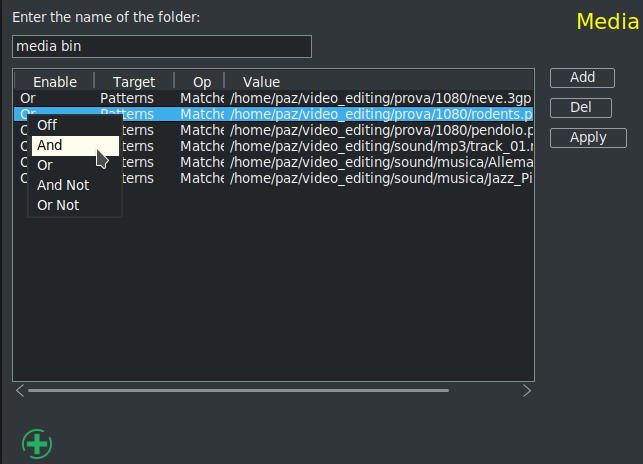
\includegraphics[width=0.8\linewidth]{modify_folder1.png}};
        \node (img2) [yshift=-1cm, xshift=3.5cm, rotate=0] at (img1) {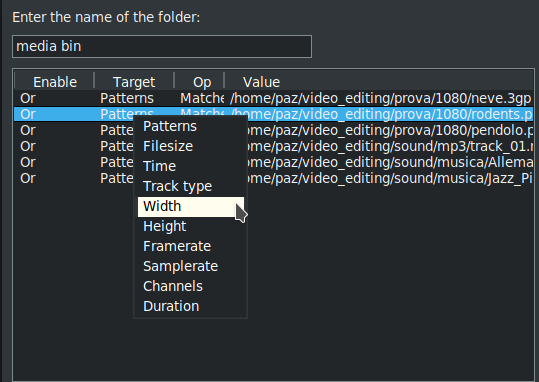
\includegraphics[width=0.8\linewidth]{modify_folder2.png}};
        \node (img3) [yshift=-1cm, xshift=3cm, rotate=0] at (img2){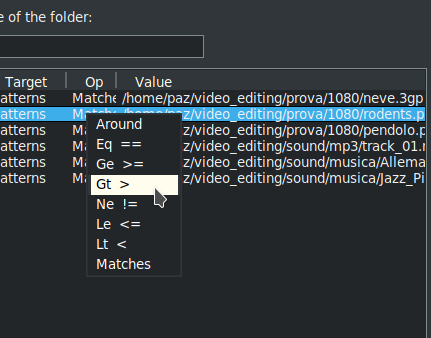
\includegraphics[width=0.5\linewidth]{modify_folder3.png}};
    \end{tikzpicture}
    \caption{The available choices for each field}
    \label{fig:modify_folder}
\end{figure}

Information about the columns and rules for the search filters in the Modify folder window follows.

Column headers:

\begin{description}
\item[ Enable]  this column is used to designate the state of that filter rule
    \begin{description}
        \item[ Off]		disable the filter
                \item[And] 		narrow your search; all of your search terms must be present
                \item[Or]		broaden your search to include more values
                \item[And Not]	exclude terms that do not contain the given value from your search results
                \item[Or Not]	include terms that do not contain the given value from your search results
    \end{description}
\item [Target] – this column designates which media asset attribute to look at
    \begin{description}
        \item[ Patterns]	each line contains a filename filter, matches the file path
                \item[Filesize]	number of bytes in a file
                \item[Time]		date file was created
                \item[Track Type]	track type of video, audio, or audio video (for both)
                \item[Width]	Format width
                \item[Height]	Format height
                \item[Framerate]	Video framerate
                \item[Samplerate]	Audio samplerate
                \item[Channels]	Number of audio channels
                \item[Duration]	Playback time in seconds -- it uses the largest of audio or video if contains both
    \end{description}
\item[Op] – boolean operators used to narrow or broaden the relationship between your search terms
    \begin{description}
        \item[Around]	about this value; use \textit{+radius} for a search range: [target–radius$\dots$  target+radius]
        \item[Eq	]	equal to
        \item[Ge]	greater than or equal to
        \item[Gt]	greater than
        \item[Ne]not equal
        \item[Le]	less than or equal
        \item[Lt] less than
        \item[Matches]	exactly matches for strings
    \end{description}
\end{description}

\textbf{Value} --- the characteristic you are looking for with expressions that can be written with the following:

\begin{description}
\item[Number] (decimal points are allowed and will be converted to a standard form):
    \begin{description}
        \item[inf] representing infinity
        \item[\#[TtGgMmKk]]  ---  where \# represents a number and the characters mean:
    \end{description}

    \begin{tabular}{rcl}
        inf&=& infinity\\
        T&=&1099511627776\\
        t&=&1000000000000\\
        G&=&1073741824\\
        g&=&1000000000\\
        M&=&1048576\\
        m&=&1000000\\
        K&=&1024\\
        k&=&1000\\
    \end{tabular}

\item[Scalar:] 

    \begin{tabular}{l}
        Number\\
        Number+Number\\
    \end{tabular}
\item[Date time:]
    \begin{tabular}{rcl}
        date&=&year/month\\
        date&=&year/month/day\\
        time&=&hour:minute\\
        time&=&hour:minute:second\\
        date\_time&=&date time\\
    \end{tabular}

  \item[Duration:]
      \begin{tabular}{rcl}
    day  &=&	\#day 	  | \#days\\
    week &=&	\#week 	  | \#weeks\\
    month&=&	\#month | \#months\\
    year &=&	\#year	  | \#years\\
    delta&=&secs\\
    delta&=&mins:secs\\
    delta&=&hours:mins:secs\\
      \end{tabular}

\item[Around time:]
    date time+duration

  \item[Around length:]
    duration+duration

\end{description}

Table showing the allowed usage:

%TODO create table for below code
\begin{lstlisting}[numbers=none]
target:    |  eq  ge  gt  ne  le  lt   matches  around
++++++++++++++++++++++++++++++++++++++++++++++++++++++++
patterns   | <---- strcmp ---------> + filter + nearest
file_size  | <---- arithmetic -------+------> + radius
mod_time   | <---- arithmetic -------+------> + radius
track_type | <---- member test ------+--------+------>
width      | <---- arithmetic -------+------> + radius
height     | <---- arithmetic -------+------> + radius
framerate  | <---- arithmetic -------+------> + radius
samplerate | <---- arithmetic -------+------> + radius
channels   | <---- arithmetic -------+------> + radius
duration   | <---- arithmetic -------+------> + radius
\end{lstlisting}

where in the above, the filter can be:

\begin{tabular}{rcl}
    filter&=&list\\
    filter&=&token\\
    list&=&[token]\\
    list&=&[token]list\\
    string&=&<chars>|<empty>\\
    token&=&string\\
    token&=&string*token\\
\end{tabular}

Examples with some caveats first:

\begin{enumerate}
    \item   \textit{Or} generally includes or adds whereas \textit{And} generally excludes or subtracts.
    \item   The filters only work on media in the folder; if there is no media, then there is nothing to search.
    \item   The examples below are not meant to be executed as a list of filters in Modify folder, they are just single line examples to indicate what can work.
    \item   Sort is by filename base name (directory path not included automatically) except when the \textit{Around} operation is used and then it is sorted by that Target distance first and then filename.
\end{enumerate}

\begin{table}[htpb]
    \centering
    \caption{Examples}
    \label{tab:label}
    \small
    \begin{tabular}{lllm{10em}m{10em}} \toprule
        Enable&	Target&	Op&	Value&	meaning\\\midrule
Or	&Patterns  &Matches   &*&	 all files from the Media folder are included\\
And Not&Filesize&Lt	&160000000& no files that are less than 160MB in size \\
Or Not&	Time	&Ge	&2018/07/30 06:13:00	& files not greater than or equal date\\
And	&Duration&Eq	&01:00		& files included must have 60 secs. Duration\\
Off	&Samplerate&Ne	&44000		& off for now, but may want to include later\\
And	&Framerate&Around&24+1		& files included all have 24 to 25 framerate\\
Or	&Patterns&Matches&[*.mp4]	& all files with the extension of mp4\\
Or	&Time&	Around&2018/08/02 06:00:00 + 02:00:00  & files at 4AM to 8 AM\\\bottomrule
    \end{tabular}
\end{table}


\subsection{Vicons \& Aicons – aka Video Icons / Audio Icons}%
\label{sub:vicons_aicons_aka_video_icons_audio_icons}

Vicons are video icons.  
Aicons are audio icons.  
By default the Resources window will play the first 5 seconds of video or audio waveform looped in the area occupied by the media icons (figure~\ref{fig:vicons1}). 
This is enabled for the Media/Proxy folders in icon mode when the mouse pointer is inside the Resources window. 

\begin{figure}[htpb]
    \centering
    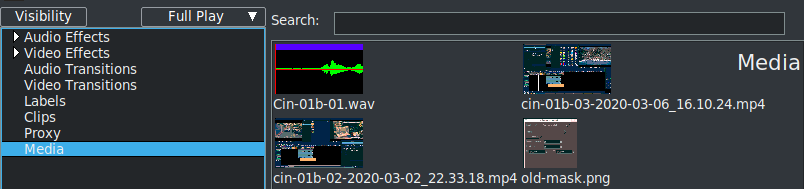
\includegraphics[width=0.99\linewidth]{vicons1.png}
    \caption{Note "Full Play" mode and Vicons and Aicons in Media folder}
    \label{fig:vicons1}
\end{figure}

The waveform in the figure~\ref{fig:vicons2} is displayed in the Resources window in the color green for the 3 audio tracks. 
There is a colored bar on the top of each a-icon where the color is based on the Color Spectrum -- the smaller the time duration, the redder the color; then as the time duration goes up, the color goes up so that you will go to green, then yellow, then blue, then really dark blue, then purple for the audio files 1 hour and over.  
There are various other colors between these colors same as that seen in the color spectrum in the screenshot below.  
Colors are utilized from the hue wheel in the counter-clockwise direction.  
Note that the horizontal line in the middle of the a-icon is yellow/red representing the 2 audio tracks and is only red for mono.



\begin{figure}[htpb]
    \centering
    %\includegraphics[width=0.8\linewidth]{name.ext}
    \begin{tikzpicture}[scale=1, transform shape]
        \node (img1) [yshift=0cm, xshift=0cm, rotate=0] {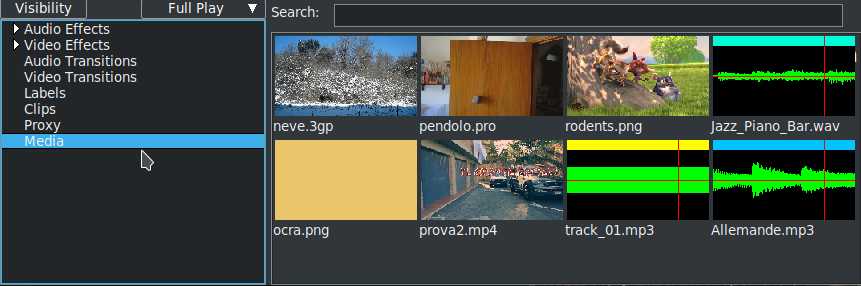
\includegraphics[width=0.99\linewidth]{vicons2.png}};
        \node (img2) [yshift=0cm, xshift=2.8cm, rotate=0] at (img1.south west) {\includegraphics[width=0.3\linewidth]{hue_wheel.png}};
        \node [yshift=-5mm, xshift=1cm,anchor=west] at (img2.east) (Arrow1) {\parbox{18em}{Color hue wheel. For illustration only}};
        \draw [->, line width=1mm] (Arrow1) edge  ([yshift=-5mm] img2.east);
    \end{tikzpicture}
    \caption{Draw Vicons   |            Screenshot display various audio file lengths; red is shortest.}
    \label{fig:vicons2}
\end{figure}

Note that if in \texttt{Settings $\rightarrow$ Preferences} under the Appearance tab, you have unchecked \textit{Use thumbnails in resource window} you will only have default icons and none of the above capabilities.


\subsection{Resources Window Preview Mode}%
\label{sub:resources_window_preview_mode}


Preview mode can be used to pop up a window which draws the vicons/aicons thumbnails in a larger size.  
Preview or \textit{draw vicons} mode is a helpful feature of \CGG{} that lets you see and/or hear the first 5 seconds of the video for identification purposes. 
The Preview mode/playback toggle is to the right of the Visibility label as seen in the screenshot above. 
Preview mode is available for the Media, Proxy, Media User Bins, and Clips but clips are only 1 image.

When \textit{Preview/draw vicons} is enabled/active, if you click on one of the video icons or an audio waveform icon, a view pops up that increases the size to 4 times the surface area larger. 
This makes it easier to see or hear if it is the media you are looking for in case you have many similar media files. 
To conserve memory, the video is stored 8\,bits per pixel which results in low image quality while the audio is 16\,bit. 
The reason for playing 5 seconds of a video for a vicon is that until the first I-frame, the media frequently does not decode properly.  
In other words, a lot of media does not begin at the \textit{beginning} point and will not be properly rendered until enough data has been read to assemble a picture.  
You can increase the thumbnail size, clarity of pixels (memory size) and color mode but it takes a lot more memory.  
Change these values in \texttt{Settings $\rightarrow$ Preferences}, Appearance tab, right hand side of the Layout section -- be aware that when you click OK, your session will re-initialize.  
You can also temporarily increase the preview mini-window by use of the mouse wheel up or down.

There are 4 options for the preview mode.

\begin{enumerate}
    \item  \emph{Full Play} is the default mode.  
        This means all of the media will automatically play when the mouse is in the Resources window and you can use the left mouse button to click on specific media to see it pop up in a larger view.  
        Audio only files do not play the audio until the icon is clicked on and the waveform aicon pops up into the 4x larger mode. 
        \emph{Full Play} includes the \emph{Mouse Over} capabilities as described below as well as the Inter-View \emph{Src Target} functions.

	\item  \emph{No Play} mode is especially useful on smaller computers and for users who find the constant loop play to be somewhat distracting.

	\item  \emph{Mouse Over} mode is activated by a single click on one of the vicons/aicons and deactivated with another single click over any of the icons.  
    Once activated, whenever you just move the mouse over an icon, it automatically pops up the increased size preview.  
    The first time in your session that you enable this feature, it may take a few seconds to load all of the icon previews into memory so be patient and just wait.  
    \emph{Mouse Over} mode makes it quick and easy to preview without having to drag the media to the viewer.  
    You can still drag the media same as without preview enabled.  

	\item  \emph{Src Target} mode gives easy access to the Inter-View source target available by using the middle mouse button on media.  
    There are 2 advantages to this mode -- there is no 5 second play loop taking up cpu time and the popup allows for the use of the letter “\texttt{f}” on that popup to have it go to fullscreen mode.  
    \emph{Src Target} mode in any scenario never plays sound as that is nonsensical usage.  
    After the initial click to pop media in this mode, you also have the \emph{Mouse over} feature.
\end{enumerate}

For any of the options, but not \emph{No Play}, you can temporarily turn off that option by clicking on the button using the middle mouse button.  
This helps to avoid having the thumbnail get in the way of dragging or other functions.  
When you do, a line will be drawn through the current preview mode so that you are aware that it is in \emph{No Play} mode until click it again.

Note that if in \texttt{Settings $\rightarrow$ Preferences} under the Appearance tab, you have unchecked \textit{Use thumbnails in resource window} you will only have default icons and no active previews.

\begin{figure}[htpb]
    \begin{minipage}{.69\linewidth}
        \centering
        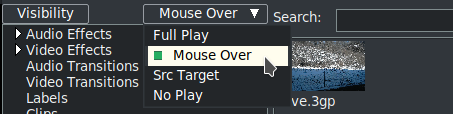
\includegraphics[width=0.99\linewidth]{preview_icon_mode.png}
        \caption{The location of the Preview/Draw Icons mode.}
        \label{fig:preview_icon_mode}
    \end{minipage}
    \hfill
    \begin{minipage}{.29\linewidth}
        \vspace{2ex}
        \centering
        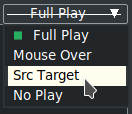
\includegraphics[width=0.7\linewidth]{line_through_mode.png}
        \caption{Note the line through the mode.}
        \label{fig:line_through_mode}
    \end{minipage}
\end{figure}



\subsection{Moving clips/media from/to Resources window}%
\label{sub:moving_clips_media_from_to_resources_window}

If you have several media files loaded into the Resources window of one instance of \CGG{} and want to load some of the same ones into another instance or just want a listing to save in a file for later use, you can do this with these set of steps:

Copy or paste a list of files in the Media Resources window:  


\begin{enumerate}
    \item  create a highlighted selection of the desired media files in the media Resources window
    \item    right click on an unused portion of that window to bring up the popup menu
    \item     select the \textit{Copy file list} item and a file list box will appear that contains the full path filenames
    \item     wipe the textbox using your standard copy/paste method to put the list of files in the copy buffer
    \item     in another \CGG{} instance, choose the \textit{Paste file list} of the media Resources window
    \item     paste the list of files, again using your standard paste method, into the new file list box; press OK
    \item    the status bar of the main window will be updated as the file list is loaded to the media folder (the purpose of displaying the status is simply to show that the load is progressing normally).
\end{enumerate}

Obviously this \textit{Paste file list} feature means you can create a list of files outside of \CGG{} using an editor, wipe the names, and then use \textit{Paste file list} to load them into the media Resources window.  

It is important to note that in the steps above, the Operating System cut and paste capabilities are in use for steps 4 and 6 as opposed to \CGG{}’s c/v shortcuts.  
Since the procedure varies among the distros, you will have to adapt to your specific one.  For example, a usage for ubuntu consists of:
\begin{enumerate}
    \setcounter{enumi}{3}
    \item   Ctrl-c to copy the list of files; open gedit; Ctrl-v to paste the list of files into gedit
    \item   Ctrl-c or the standard way using the right click to copy this list from gedit
    \item Ctrl-v paste the list of files into the new file list box, and press OK
\end{enumerate}

\begin{figure}[htpb]
    \centering
    \begin{minipage}{.9\linewidth}
    \centering
        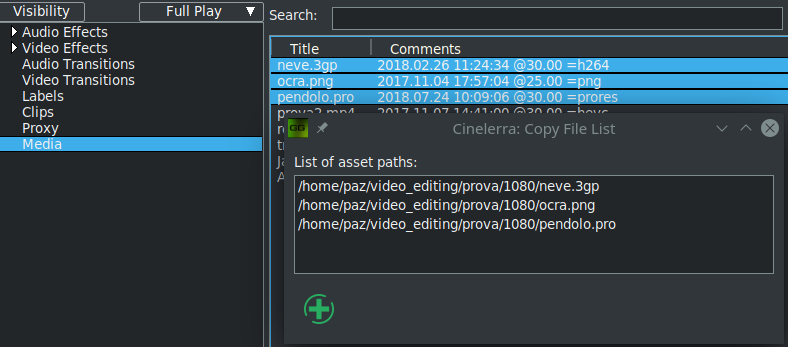
\includegraphics[width=0.99\linewidth]{copy_files1.png}
    \end{minipage}
    \vfill
    \begin{minipage}{.5\linewidth}
    \centering
        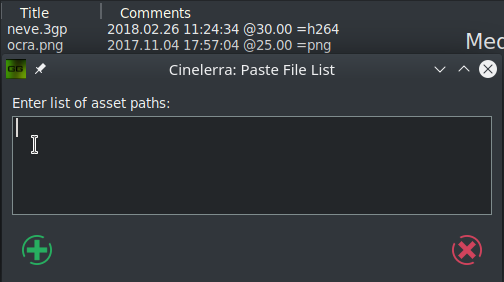
\includegraphics[width=0.99\linewidth]{copy_files2.png}
    \end{minipage}
    \caption{Example of copy file list}
    \label{fig:copy_files1}
\end{figure}

In the Figure~\ref{fig:copy_files1}, one instance of \CGG{} has 3 items in the Media area highlighted that were copied to the file list.  
Note how it includes the full pathname.

In this screenshot on another instance of \CGG{}, there are only 2 items in the media but the \textit{Paste file list} box is ready to have the items inserted via the standard text box paste method.  When that is done, the additional 6 media files will be available on this other instance too.


Another possible usage of this capability:

\begin{enumerate}
    \item  Right Click on the Clips Resources window and use the \textit{Paste Clip} option to paste the Copy selection as a clip.  
    \item  Similarly, by highlighting a clip in the Resources window and selecting its copy popup menu item using the right mouse button, that copy buffer can now be loaded onto the timeline.
\end{enumerate}


\subsection{Snapshot / Grabshot}%
\label{sub:snapshot_grabshot}

\begin{figure}[htpb]
    \centering
    \begin{minipage}{.49\linewidth}
    \centering
    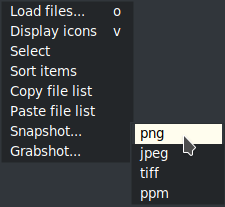
\includegraphics[width=0.8\linewidth]{snapshot.png}
    \caption{Snapshot menu and choices}
    \label{fig:snapshot}
    \end{minipage}
    \begin{minipage}{.49\linewidth}
    \centering
    \begin{tikzpicture}[scale=1, transform shape]
        \node (img1) [yshift=0cm, xshift=0cm, rotate=0] {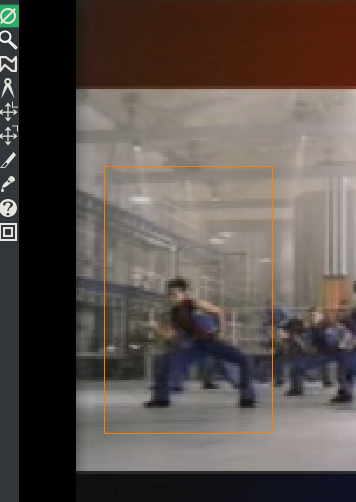
\includegraphics[width=0.65\linewidth]{grabshot.png}};
        \node (img2) [yshift=2cm, xshift=-1cm, rotate=0] {\includegraphics[width=0.07\linewidth]{reticle.png}};
    \end{tikzpicture}
    \caption{Grabshot reticle \& orange box}
    \label{fig:grabshot_recticle}
    \end{minipage}
\end{figure}

To take a snapshot, perform the following steps:

\begin{enumerate}
    \item set your timeline insert marker where you want the snapshot -- this frame shows in the compositor
    \item  right click in an empty spot in the media folder and the popup shows snapshot as the $5^{th}$ item down
    \item  highlight that and the submenu comes up allowing you to choose png, jpg, ppm or tiff
\end{enumerate}

The snapshot shows up in the Media folder.  
It is saved by default in \texttt{/tmp} as

\texttt{snap\_date-time.ext} BUT you can change the default directory path in \texttt{Settings $\rightarrow$ Preferences $\rightarrow$ Interface tab} in the right hand side of the Editing section.

Grabshot is the $6^{th}$ menu item.  
A red circle reticle can be moved to the area to grab; use left mouse drag to surround an area; and right click to grab.




\section{Other Options and Other Windows}%
\label{sec:other_options_and_other_windows}

\subsection{Transport Controls}%
\label{sub:transport_controls}

Transport controls are useful for navigation and for playing media.  
Each of the Viewer, Compositor, and Program windows has its own transport panel.  
The controls generally all contain a yellow colored tooltip when you mouse over the control, providing a hint of their function and shortcuts for usage.

The transport panel is controlled by the keyboard as well as the graphical interface. 
For each of the operations it performs, the starting position is the position of the insertion point in the Program window and the slider in the Compositor and Viewer windows. 
The ending position is either the end or start of the timeline or the end or start of the selected region if there is one.

The orientation of the end or start depends on the direction of playback. 
If it is forward the end position is the end of the selected region. 
If it is backward the end position is the start of the selected region.  
The insertion point moves to track playback. 
When playback stops, the insertion point stays where playback stopped. 
Thus, by playing back you change the position of the insertion point. 
The keyboard interface of either the numeric pad or alternative keys has more speeds with the addition of \emph{Forward Slow}(2) and \emph{Reverse Slow} (5).  
Hitting any key on the keyboard twice pauses it. 
The shortcuts section of this manual as well as a Shell Command available from the \CGG{} main window has a listing of each of the keys.

When using frame advance functions the behavior may seem odd. 
If you frame advance forward and then frame advance backward, the displayed frame does not change. 
This is because the playback position is not the frame but the time between two frames. 
The rendered frame is the area that the playback position crosses. 
When you increment the time between two frames by one and decrement it by one, you cross the same frame both times and so the same frame is displayed.  
There is an option in \texttt{Settings $\rightarrow$ Preferences, Appearance tab} to \textit{Always show next frame} that may help make this clearer for some users.

The transport behavior changes if you hold down Ctrl when issuing any of the transport commands. This causes the starting point to be the In point if playing forward and the Out point if playing backward. If playing forward, the Out point becomes the ending point and if playing backward, the In point becomes the ending point. If no In/Out points are specified, the behavior falls back to using the insertion point and track boundaries as the starting and ending points.

The transport behavior also changes if you hold down the Shift key along with KeyPad 1--6.  
If normally audio is included in the play, it will be removed and if normally audio is not included in the play, it will be added.


\subsection{Zoombar}%
\label{sub:zoombar}

The compositor has zoom capability. 
The pull-down menu on the bottom of the compositor window has a number of zoom options. 
When set to Auto the video is zoomed to match the compositor window size as closely as possible. 
When the video is zoomed bigger than the window size,  you can use scrollbars to scan around or if the zoom icon is enabled, the middle mouse button can be used to zoom in or out the video.

The zoom toggle also causes the Compositor window to enter zoom mode. 
In zoom mode, clicking in the video output zooms in while a Ctrl-click in the video output zooms out. 
If you have a wheel mouse, rotating the wheel zooms in or out too. 
Zooming in or out with the zoom tool does not change the rendered output. 
It is merely for scrutinizing video or fitting it in the desktop. Playing video on the compositor when zoomed to any size other that 100\%, the original size, requires \CGG{} to do extra processing steps. 
This could affect performance on slower systems

\subsection{Show Overlays}%
\label{sub:show_overlays}

Color Coded Keyframe Curves are a big feature in the \textit{Show Overlays} window because by changing the colors to suit the user, it helps to remove confusion from multiple curves on the track canvas.  
They can be viewed from the pulldown menu of \texttt{Window $\rightarrow$ Show overlays} but they will operate the same as when used from the View pulldown menu.  
The \textit{Color Coded Keyframe Curves} have distinct colors associated with each type for ease of identification.  
By clicking LMB on the \textit{Color Ball} to the right of any keyframe type in the \textit{Show overlays} menu you have the ability to change the colors to whatever works best for your video.  
The color ball changes made will be retained across sessions.

There is a line separating the first 4 items, which are just non-automation type settable values as opposed to \textit{auto} keyframe types.  
The color is not changeable for the 3 items of Mode, Pan, and Mask which simply display their symbol icon.

Figure~\ref{fig:overlays_window} displays the Show overlays popup with all of its options and color coded types such as yellow for Speed and blue for Camera Z.  
Upon clicking on the associated \textit{color ball} to the right of any keyframe type, for example \textit{Fade} in this screenshot, the color wheel palette window pops up so that you can manipulate the color as desired.

\begin{figure}[htpb]
    \centering
    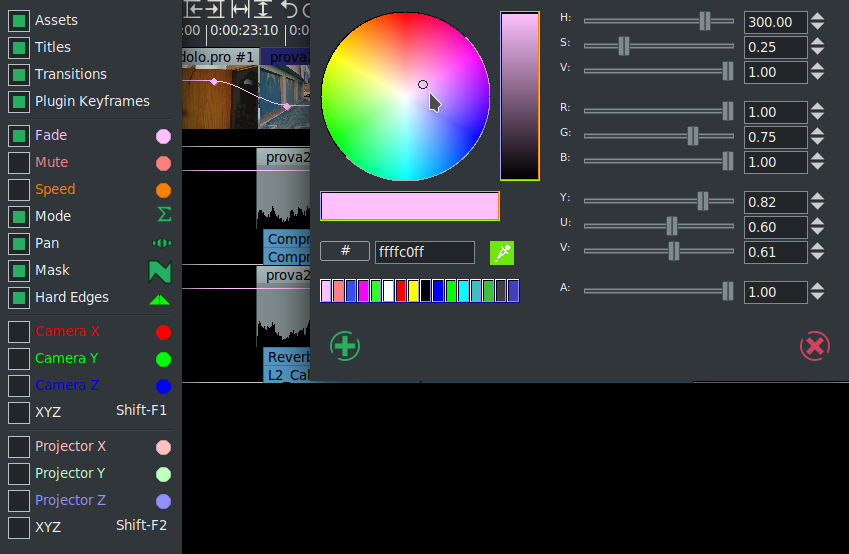
\includegraphics[width=0.85\linewidth]{overlays_window.png}
    \caption{Show Overlays window on the left with the Color ball window to the right to set color}
    \label{fig:overlays_window}
\end{figure}

Figure~\ref{fig:overlays1} shows several color coded lines for different keyframes along with the Fade slider for manipulation.  
The slider is in the same color as the color coded keyframe type line which is the same color as in the \textit{Show overlays} window.

\begin{figure}[htpb]
    \centering
    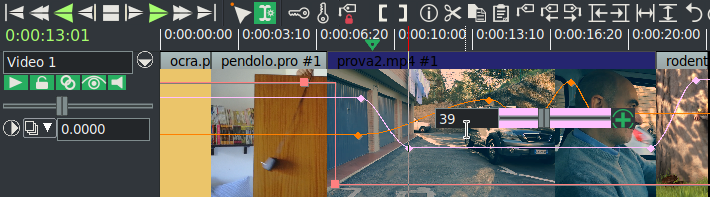
\includegraphics[width=1.0\linewidth]{overlays1.png}
    \caption{Lines are colored here on the timeline as designated in Show Overlays}
    \label{fig:overlays1}
\end{figure}

Overlays Window Nuances:

The Overlays window is an alternative to the main track canvas View pulldown, and thus the order is mostly maintained to match each other.  
To make it easier to get a quick temporary look at a specific option, there is a shortcut of Shift-LMB (left mouse button) that can be used as opposed to having to uncheck everything that is currently checked and then having to recheck them on when done.  
Here is a list of how they work.  Keep in mind that if the Expander on the patchbay is enabled, you still see the track.

\begin{itemize}
    \item  Shift+LMB (left mouse button) in the Overlays Window on a checkbox will turn off all other
        checkboxes except for the one you are on.  Then this named box will have outline for a  \textit{hot} spot.
    \item  Shift+LMB on this \textit{hot} spot will return to \textit{cool} of the previous settings with all of the previous
        checkboxes checked again.
\end{itemize}

\begin{figure}[htpb]
	\begin{minipage}{.29\linewidth}
		\centering
		\includegraphics[width=0.99\linewidth]{overlays_list1.png}
		\caption{Original Settings --- cool spot}
		\label{fig:overlays_list1}
	\end{minipage}
	\hfill
	\begin{minipage}{.29\linewidth}
		\centering
		\includegraphics[width=0.99\linewidth]{overlays_list2.png}
		\caption{Note Titles box hot spot  }
		\label{fig:overlays_list2}
	\end{minipage}
	\hfill
	\begin{minipage}{.29\linewidth}
		\centering
		\includegraphics[width=0.99\linewidth]{overlays_list3.png}
		\caption{Cam/Proj XYZ toggle to fine tune}
		\label{fig:overlays_list3}
	\end{minipage}
\end{figure}

\begin{itemize}
    \item  Shift+LMB on a non-\textit{hot} spot will simply check or uncheck a box and there is no previous state.
    \item This all works in conjunction with the View pulldown menu which, of course, has no hot spots.
    \item  Caveat \#1 - Shift+LMB on the top 4 choices of Assets, Titles, Transitions, Plugin Keyframes will turn
        off all of the checkboxes below because it makes sense to do so.
    \item  Caveat \#2 - Shift+LMB on the Autos will not turn off Assets, Titles, Transitions, or Plugin Keyframes
        because you need to be able to see what is going on.
        \item Caveat \#3 - XYZ toggle on/off of Camera and Projector are not affected.
\end{itemize}




\subsection{Sound Level Meters Window}%
\label{sub:sound_level_meters_window}

An additional window, the levels window, can be brought up from the Window pulldown.  
The levels window displays the output audio levels after all mixing is done.  
The visible range of the sound level meters is configurable in \texttt{Settings $\rightarrow$ Preferences, Interface tab} under the Operations section.

\begin{wrapfigure}[18]{O}{0.3\linewidth} 
	\centering
	\vspace{-2ex}
	\includegraphics[width=0.5\linewidth]{volume_meter.png}
	\caption{Sound Level Meters Window}
	\label{fig:volume_meter}
\end{wrapfigure}

Sound level meters can be toggled in the viewer and compositor windows with the show meters button.  
They also appear in the patchbay when the track is expanded and in the recording monitor when audio is being recorded. 

The sound levels in the levels window, compositor, and viewer correspond to the final output levels before they are clipped to the sound card range.  
In the record monitor they are the input values from the sound card.  
In the patchbay they are the sound levels for each track after all effects are processed and before down-mixing for the output.  
Most of the time, audio levels have numerical markings in dB but in the patchbay there is not enough room.

The sound level is color coded as an extra means of determining the sound level.  
Even without numerical markings, the sound level color can distinguish between several ranges and overload.  
Look at the color codings in a meter with numerical markings to see what colors correspond to what sound level.  
Then for meters in the patchbay in expanded audio tracks, use the color codings to see if it is overloading.

Be aware that sound levels in \CGG{} can go above 0 dB.  
This allows for not only seeing if a track is overloading but how much information is being lost by the overloading.  
Overloading by less than 3 dB is usually acceptable.  
While overloading is treated as positive numbers in \CGG{}, it is clipped to 0 when sent to a sound card or file.


%%% Local Variables:
%%% mode: latex
%%% TeX-master: "../CinelerraGG_Manual"
%%% End:

\chapter{Project and Media Attributes}%
\label{cha:project_and_media_attributes}

When you play media files in \CGG{}, the media files have a certain number of tracks, frame size, sample size, and so on. 
No matter what attributes the media file has, it is played back according to the project attributes. 
So, if an audio file's sample rate is different than the project attributes, it is resampled. 
Similarly, if a video file's frame size is different than the project attributes, the video is composited on a black frame, either cropped or bordered with black.

The project attributes are adjusted in Settings $\rightarrow$ Set Format (figure~\ref{fig:set-format}) or can be created in File $\rightarrow$ New. 
When you adjust project settings in File $\rightarrow$ New, a new empty timeline is created. 
Every timeline created from this point on uses the same settings. 
When you adjust settings in Settings $\rightarrow$ Format, media on the timeline is left unchanged. 
But every timeline created from this point uses the same settings.

\begin{figure}[htpb]
	\centering
	\includegraphics[width=0.5\linewidth]{images/set-format.png}
	\caption{Set Format window - note the Audio Channel positions}
	\label{fig:set-format}
\end{figure}

In addition to the standard settings for sample rate, frame rate, and frame size, \CGG{} uses some less traditional settings like channel positions, color model, and aspect ratio.  
The aspect ratio refers to the screen aspect ratio.

Edit decision lists , the EDL stored in XML, save the project settings.  
Formats which contain media but no edit decisions just add data to the tracks. 
Keep in mind details such as if your project sample rate is 48\,kHz and you load a sound file with 96\,kHz, you will still be playing it at 48\,kHz.  
Or if you load an EDL file at 96\,kHz and the current project sample rate is 48\,kHz, you will change it to 96\,kHz.

The New Project window has some options that are different than the Set Format window as you can see by comparing figure~\ref{fig:set-format} above with this figure~\ref{fig:new-project}. 
Mostly notably is the field for a directory path and a Project Name.

\begin{figure}[htpb]
	\centering
	\includegraphics[width=0.5\linewidth]{images/new-project.png}
	\caption{New Project dialog window}
	\label{fig:new-project}
\end{figure}

Explanation of the various fields is described next.

\section{Audio attributes}%
\label{sec:audio_attributes}


\begin{description}
            \item[Presets:]
            select an option from this menu to have all the project settings set to one of the known standards.  Some of the options are 1080P/24, 1080I, 720P/60, PAL, NTSC, YouTube, and CD audio.
            
            \item[Tracks:]
            (in New Project menu only) sets the number of audio tracks for the new project. Tracks can be added or deleted later, but this option is on the New Project menu for convenience.
            
            \item[Samplerate:]
            sets the samplerate of the audio. The project samplerate does not have to be the same as the media sample rate that you load. Media is resampled to match the project sample rate.
            
            \item[Channels:]
            sets the number of audio channels for the new project. The number of audio channels does not have to be the same as the number of tracks.
            
            \item[Channel positions:]
            the currently enabled audio channels and their positions in the audio panning boxes in the track patchbay are displayed in the channel position widget in the Set Format window.  
            You can see this display on the left side in figure~\ref{fig:set-format} above. 
            Channel positions are not in New Project window.
            
            The channels are numbered. 
            When rendered, the output from channel 1 is rendered to the first output track in the file or the first sound card channel of the sound card. 
            Later channels are rendered to output tracks numbered consecutively. 
            The audio channel positions correspond to where in the panning widgets each of the audio outputs is located. 
            The closer the panning position is to one of the audio outputs, the more signal that speaker gets. 
            Click on a speaker icon and drag to change the audio channel location. 
            The speakers can be in any orientation. 
            A different speaker arrangement is stored for every number of audio channels since normally you do not want the same speaker arrangement for different numbers of channels.
            
            Channel positions is the only setting that does not affect the output necessarily. 
            It is merely a convenience, so that when more than two channels are used, the pan controls on the timeline can distinguish between them. 
            It has nothing to do with the actual arrangement of speakers. 
            Different channels can be positioned very close together to make them have the same output.
            
\end{description}

\section{Video attributes}%
\label{sec:video_attributes}

\begin{description}
    \item[Tracks:]
        (in New Project menu only) sets the number of video tracks the new project is assigned. 
        Tracks can be added or deleted later, but options are provided here for convenience.

    \item[Framerate:]
        sets the framerate of the video. 
        The project framerate does not have to be the same as an individual media file frame rate that you load. 
        Media is reframed to match the project framerate.

    \item[Canvas size:]
        sets the size of the video output. 
        In addition, each track also has its own frame size. 
        Initially, the New Project dialog creates video tracks whose size match the video output. 
        The video    track sizes can be changed later without changing the video output.

    \item[Aspect ratio:]
        sets the aspect ratio; this aspect ratio refers to the screen aspect ratio. 
        The aspect ratio is applied to the video output. 
        The aspect ratio can be different than the ratio that results from the formula: $\dfrac{h}{v}$ (the number of horizontal pixels divided into the number of vertical pixels). 
        If the aspect ratio differs from the results of the formula above, your output will be in non-square pixels. 

    \item[Auto aspect ratio:]
        if this option is checked, the Set Format dialog always recalculates the Aspect ratio setting based upon the given Canvas size. This ensures pixels are always square.

    \item[Color model:]
        the internal color space of \CGG{} is X11 sRGB without color profile. \CGG{} always switches to sRGB when applying filters or using the compositing engine. Different case for decoding/playback or encoding/output; the project will be stored in the color model video that is selected in the dropdown.  
        Color model is important for video playback because video has the disadvantage of being slow compared to audio.  
        Video is stored on disk in one colormodel, usually a YUV derivative. 
        When played back, \CGG{} decompresses it from the file format directly into the format of the output device. 
        If effects are processed, the program decompresses the video into an intermediate colormodel first and then converts it to the format of the output device. 
        The selection of an intermediate colormodel determines how fast and accurate the effects are.  
        A list of the current colormodel choices follows.

        \begin{description}
            \item[RGB-8 bit] 
                Allocates 8\,bits for the R, G, and B channels and no alpha. This is normally used for uncompressed media with low dynamic range.
            \item[RGBA-8 bit]
                Allocates an alpha channel to the 8\,bit RGB colormodel. It can be used for overlaying multiple tracks.\\
            \item[RGB-Float]
                Allocates a 32\,bit float for the R, G, and B channels and no alpha. This is used  for high dynamic range processing with no transparency.
            \item[RGBA-Float]
                This adds a 32\,bit float for alpha to RGB-Float. It is used for high dynamic range processing with transparency. Or when we don't want to lose data during workflow, for example in color correction, key extraction and motion tracking. \\
            \item[YUV-8 bit]
                Allocates 8\,bits for Y, U, and V. This is used for low dynamic range operations in which the media is compressed in the YUV color space. Most compressed media is in YUV and this derivative allows video to be processed fast with the least color degradation.
            \item[YUVA-8 bit]
                Allocates an alpha channel to the 8\,bit YUV colormodel for transparency.
        \end{description}       
                In order to do effects which involve alpha channels, a colormodel with an alpha channel must be selected. 
                These are RGBA-8 bit, YUVA-8 bit, and RGBA-Float. 
                The 4 channel colormodels are slower than 3\,channel colormodels, with the slowest being RGBA-Float. 
                Some effects, like fade, work around the need for alpha channels while other effects, like chromakey, require an alpha channel in order to be functional.  
                So in order to get faster results, it is always a good idea to try the effect without alpha channels to see if it works before settling on an alpha channel and slowing it down.

                When using compressed footage, YUV colormodels are usually faster than RGB colormodels. 
                They also destroy fewer colors than RGB colormodels. 
                If footage stored as JPEG or MPEG is processed many times in RGB, the colors will fade whereas they will not fade if processed in YUV.  
                Years of working with high dynamic range footage has shown floating point RGB to be the best format for high dynamic range. 
                16 bit integers were used in the past and were too lossy and slow for the amount of improvement.  
                RGB float does not destroy information when used with YUV source footage and also supports brightness above 100\,\%. 
                Be aware that some effects, like Histogram, still clip above 100\,\% when in floating point.
        
    \item[Interlace mode:]
        this is mostly obsolete in the modern digital age, but may be needed for older media such as that from broadcast TV.  Interlacing uses two fields to create a frame. One field contains all odd-numbered lines in the image; the other contains all even-numbered lines.  Interlaced fields are stored in alternating lines of interlaced source footage. The alternating lines missing on each output frame are interpolated.
\end{description}





\chapter{Load, Save, and the EDL}%
\label{cha:load_save_and_the_EDL}

There are many supported file formats that can be loaded and rendered to, that is to say, imported and exported. 
The format of the file affects what \CGG{} does with it.  
Some file formats are very slow to display on the timeline, especially video which is highly compressed.  
Drawing video thumbnails, picons, on the timeline can be very slow.  (You can disable picon drawing for these files with the \textit{draw media} toggle in the patchbay to speed up operations).

\section{EDL --- Edit Decision List}%
\label{sec:edl_edit_decision_list}

When \CGG{} saves a file, it saves the EDL, Edit Decision List, of the current project but does not save any media. 
Edit decision lists, more commonly referred to as the EDL, are generated by \CGG{} for storing projects.  
The EDL contains all the project settings and locations of every edit. 
Instead of media, the file contains pointers to the original media files on disk.  
EDL files are specific to \CGG{}.    

The EDL files generally have an extension of \texttt{.xml}.  
The purpose of the EDL is to separate the media from all of the editing operations so that the original media remains intact. 
When the \texttt{.xml} file is loaded, changes to the attributes of the current project are made based on the EDL\@. Edit decision lists are text files which means they can be edited in a text editor.  EDL and XML are used interchangeably.

\section{Supported File Formats}%
\label{sec:supported_file_formats}

There are basically 2 kinds of supported file formats, native and ffmpeg.  With the addition of ffmpeg, the majority of the supported file formats you will be using comes via this thirdparty package.  There are hundreds of ffmpeg file format and codec combinations. This set of possibilities includes qt (quicktime), avi (audio-video interleave),  mp4, mp3, mov, mpeg, m2ts, ts, wmv, mts, mpg, flv, mkv, webm, webp, ProRes and many more.

The other supported formats, referred to as \textit{native},  include the following:
AC3, 
Apple/SGI AIFF,
Sun/NeXT AU,
FLAC ,
Microsoft WAV,
Raw DV and PCM,
MPEG Audio and Video.

\paragraph{Still Images:}  JPEG/EXR/PNG/PPM/TGA/TIFF

\paragraph{MPEG Files:} 
What is an MPEG file?  A very common file format is MPEG because it works with many cameras and televisions.  Mpeg2 video, an elementary codec stream for mpeg files, is the most common format.  To read this format you need to decode the mpeg stream.  You can read and write mpeg natively.  Mpeg video encoding is done separately from mpeg audio encoding when using the native file format, meaning that 2 passes are required and then they have to be muxed together.  However, if using ffmpeg it is rendered in only 1 pass.  DVD uses MPEG as does NTSC and Pal.

\subsection{Working with Still Images}%
\label{sub:working_with_still_images}

Still images are played from 1 to any number of times, over and over; they have no duration. You can load still images on video tracks just like you do for any video file. When loaded on the track, use the down arrow on the timeline so you can see the single frame. To extend the length of the image, drag its boundaries just as you would do with regular video media. You can drag the boundaries of a still image as much as you want. Images in \CGG{} have the ability to be dragged to an infinite length. Alternatively, you can define the initial length of the loaded images. The parameter is set in the Images section of the \texttt{Settings $\rightarrow$ Preferences $\rightarrow$ Recording} window.

Unless your original material comes from a digital source using its best resolution (like a digital camera), the first thing you might have to do before you can use it is to somehow capture the assets into a usable digital medium. For old photos, paper maps, drawings or diagrams, you can scan them into a file format like PNG, TIF, TGA or JPG files by using a digital scanner.

Rendering a video to a single image causes the final image file to be overwritten for every timeline position. The rendered file is a single still image of the last frame of the video.

\subsection{Timelapse Sequence of Images, and Animation}%
\label{sub:timelaps_sequence_images_animation}

The next areas covered in this section are the following: 
\nameref{ssub:filelist_format} such as jpeglist and \nameref{ssub:image2ffmpeg}.

In order to be reasonably fast to use, you will most likely want to prepare them by creating a script and then load by utilizing this file generated script.

\subsubsection{Filelist format}%
\label{ssub:filelist_format}

An image sequence is a series of ordered still pictures; for example a bunch of camera shots, frames of an animated scene, or series of frame shots. These can be loaded as multiple files. For timelapse sequences, as the size of camera images increases to 70 megabytes and beyond, and more images can be stored on a memory stick, more cache, memory, and system resources (such as file descriptors) are used by \CGG{} to load the images when you use the \textit{concatenate tracks} or \textit{paste at insertion point} strategies.  It is very time consuming and resource consuming when each of the image files is loaded and concatenated as edits, and it also plays super poorly.  Here is an alternative to the usual \textit{load}.  This technique may also be useful for just a bunch of pictures.

File lists formats can be utilized in some way for the following list of types of \textit{Sequence files}  The first line of the sequence list file identifies the list codec.

%\vspace*{1ex}


\begin{center}
    \begin{tabular}{l l l l}
    PNGLIST = *.png	&	PPMLIST = *.ppm	&	TGALIST = *.tga	  &  TIFFLIST = *.tiff \\
    EXALIST = *.exa	&	CR2LIST = *.cr2	&	JPEGLIST = *.jpg	&    GIFLIST = *.gif
    \end{tabular}
\end{center}

%\vspace*{1ex} 
Using the example of jpeg’s, the jpeg list sequence file type is the easiest and fastest way to access a sequence of jpg images as a single asset.  First build a jpeglist sequence file and name it something like jpeglist.sh.  There is an example script of how to do this in the Auxiliary Programs section of the Appendix (\ref{sec:image_sequence_creation}).  Once the jpeglist.sh file is built you can then run it similar to this line:

\begin{lstlisting}[style=sh]
jpeglist.sh   /<path>/file.jpg   /<path>/DSC*.jpg
\end{lstlisting}

\vspace*{1ex} \noindent If <\texttt{path}> is the same on both outfile and infiles, then file.jpg is created in the same directory as infiles, the directory contains the entire asset, and the file list uses relative paths; otherwise the file list contains absolute paths.   Since this creates outfile list as a single asset, the memory demand and access time is much lower.  When you load the outfile in \CGG{}, you will need to set \textit{Try ffmpeg last} since ffmpeg does not work with jpeglist sequence files.

An example output file from running this script residing in the directory where \texttt{DSC*.jpg} files exist is shown below.

To use this, turn off ffmpeg probes first, and open \texttt{timelapse.jpg} using File $\rightarrow$ Load files.

\begin{lstlisting}[style=sh,caption={Example: timelapse.jpg},captionpos=t]
JPEGLIST
# First line is always JPEGLIST
# Frame rate:
29.970030
# Width:
6016
# Height:
4016
# List of image files follows
./DSC04948.jpg
./DSC04949.jpg
./DSC04950.jpg
./DSC04951.jpg
...(files in between)
./DSC04997.jpg
./DSC04998.jpg
\end{lstlisting}

\subsubsection{Image2ffmpeg}%
\label{ssub:image2ffmpeg}

Image2file format is an alternative method to open an image sequence via ffmpeg.  To do this, create 2 files in the same directory as the \texttt{DSC*.jpg} files named:  \texttt{DSC0\%04d.opts}, and \texttt{DSC0\%04d.jpg}. 
\texttt{DSC0\%04d.opts} should contain the following lines which have to be modified to fit your exact requirements for duration, start\_number, and frame\_rate.


\begin{lstlisting}[style=sh,caption={Example
    DSC0\%04d.opts},captionpos=t]
loglevel=verbose
threads=auto
format=image2
codec=mjpeg 
start_number=4948
frame_rate=29.97
duration=17.36
\end{lstlisting}

Example of the contents of the file \texttt{DSC0\%04d.jpg} would be just a single line as:  JPEG
In this case, make sure \textit{Try ffmpeg first} is enabled, and load \texttt{DSC0\%04d.jpg}.  
This will access the media using ffmpeg which is slower so be patient.

\subsection{Raw Image Format of Some Digital Cameras \& Probe Order}%
\label{sub:raw_image_format_digital_camera_probe_order}

\textit{Note: requires some expert knowledge.}  Raw digital camera images are a special kind of image file that \CGG{} can load. Dcraw, as used by \CGG{}, is Dave Coffin’s open-source computer program which reads many raw-image formats typically produced by many earlier and current digital cameras.  Currently over 700 of the types of cameras it recognizes are listed at:

\hspace{4em}	{\small \url{https://www.dechifro.org/dcraw/}}

For example, included are numerous models of Canon, Fuji, Kodak, Nikon, Olympus, and Panasonic as well as many others.  Because ffmpeg tries to load \textit{any and every} file if \textit{Try Ffmpeg first} is enabled, it will make an attempt to load Raw Camera files first before any other file driver gets the chance.  In addition, there is the possibility that dcraw could conflict with the standard TIFF format, since it might be seen as format type \textit{tiff-pipe}.  Therefore it is necessary to specifically enable CR2 and either move it to the top or disable \textit{FFMPEG\_Early} and enable \textit{FFMPEG\_late} in the \textit{Probe Order} as described in another section (\ref{sub:probe_order_loading_media} and \ref{sec:ffmpeg_early_probe_explanation}).  These changed settings will be retained across \CGG{} sessions in \texttt{.bcast5}.  Usage of Raw Camera mode generally requires more in depth knowledge of your specific camera.

The first screenshot in figure~\ref{fig:raw} as in \texttt{Settings $\rightarrow$ Preferences $\rightarrow$ Playback A} Tab, shows the default checked settings of \textit{Interpolate CR2 images} and \textit{White balance CR2 images} which display the raw images in a way that you expect.  However, you may want to uncheck them to ensure that no program manipulation has modified your images so that you can add plugins or make your own modifications.  Unchecked indicates that the images are as closest as possible to unadulterated raw.

The second screenshot showing CR2 for Raw Camera highlighed/enabled in the Preferences Probes’ screen.

The final screenshot showing the Resources Asset Info displaying the File format as Raw Camera.

\begin{figure}[htpb]
    \centering
    \includegraphics[width=0.95\linewidth]{raw.png}
    \caption{Screenshots for RAW images}
    \label{fig:raw}
\end{figure}

\section{Loading Files}%
\label{sec:loading_files}

All data that you work with in \CGG{} is acquired either by loading from disk or recording from a device. This section describes loading.  To bring up the Load window go to the File pulldown and choose Load Files  (figure~\ref{fig:load}).  Next \textit{Select files to load}, and click ok (the green checkmark) or \textit{Apply}. When you use the Apply button, the Load window remains active for easily loading more files later.  Depending on the setting of the Insertion Strategy list box, your file will be either loaded directly on the Program window or in the Resources Media window.  If the file is a still image, the project's attributes are not changed and the first frame of the track becomes the image. \CGG{} usually builds an index file if one does not already exist, in order to speed up drawing. You can edit and play the file while the index is being built.

\begin{figure}[htpb]
    \centering
    \includegraphics[width=0.9\linewidth]{load.png}
    \caption{Load file menu.  Note the green checkmark for OK and the middle Apply option}
    \label{fig:load}
\end{figure}

\vspace{1ex} \noindent To load a file, you will need to:

\begin{enumerate}
    \item set a directory path in the Directory input box
    \item choose a file or set of files by highlighting your selection
    \item select an insertion strategy for loading the file 
\end{enumerate}

\noindent Once you have completed making your choices and clicking OK or Apply, by default three things occur:

\begin{itemize}[noitemsep]
    \item The existing project is cleared from the screen.
    \item The project's attributes are changed to match the file's attributes.
    \item The new file's tracks are created in the timeline.
\end{itemize}

\noindent Let's now see in detail the options of loading files.

\begin{description}
    \item[Insertion Strategy] 
    \CGG{} lets you change what happens when you load a file.  In the Load dialog window go to the Insertion strategy box and select one of the options in the drop down menu. Each of these options loads the file a different way.
    
    \begin{description}
       \item [Replace current project:] all tracks in the current project are deleted and a set of new tracks are created to match the source file.  Project attributes are only changed when loading XML\@. If multiple files are selected for loading, \CGG{} adds a set of new tracks for each file. New resources are created in the Resources Window, replacing the current ones.
       \item [Replace current project and concatenate tracks: ] same as replace current project, except that if multiple files are selected, \CGG{} will concatenate the tracks of each file, inserting different source files in the same set of tracks, one after another, in alphanumeric order, starting at 0. New resources are created in the Resources Window, replacing the current ones.  Files go across the timeline.
    \end{description}
    For ffmpeg and mpeg files, when the Insertion strategy methodology in the \texttt{File $\rightarrow$ Load files} pulldown is chosen to be either \textit{Replace current project} or \textit{Replace current project and concatenate tracks}, the basic session format parameters are reinitialized to match new media.  This selects the default asset and determines its width, height, and video length, frame rate, calculates the colormodel, and assumes square pixels to make an intelligent guess about aspect ratio for video.  For audio, the sample rate, audio length, and channel count (mono, stereo, or 5.1) are reinitialized.  In addition the \textit{Track Size} will be computed and is reinitialized to match the new loaded media.  When using \textit{replace} type insertion strategy, the new asset list is the only media in use so that this update saves the user from immediately needing to change the session format to match the only possibility.
    \begin{description}
        \item[Append in new tracks:] the current project is not deleted and new tracks are created for the source, one set of tracks for each file. New resources are created in the Resources Window.  Files go down tracks.
        \item[Concatenate to existing tracks:]  the current project is not deleted and new files are concatenated to the existing armed tracks, inserted in the same set of tracks of the current project, one after another, in     alphanumeric order, starting at the end of the tracks. If the current project has more tracks than the source, the source file will be inserted in the first set of armed tracks. If no tracks are armed, no files will be inserted. New resources are created in the Resources Window.
        \item[Paste at insertion point:] the file is pasted into the timeline at the insertion point, on the first set of armed tracks.  If multiple files are selected for loading, they will be inserted on the same set of tracks, one after the other. New resources are created in the Resources Window.
        \item[Create new resources only:] the timeline is unchanged and new resources are created in the Resources Window only.
        \item[Nest sequence:] nested assets are added to the timeline by using the Nest sequence insertion strategy.
        The file will be pasted into the timeline over the current selection or at the insertion point. A nested sequence is media that had already been saved as an EDL earlier.  Nesting is described more fully in section \ref{sec:nesting_clips_and_assetts}.
    \end{description}
    The insertion strategy is a recurring option in many of \CGG{}'s functions. In each place the options do the same thing. If you load files by passing command line arguments to \CGG{}, the files are loaded with \textit{Replace current project} by default.
    \item[Loading Multiple Files] In the Load dialog go to the list of files. Selecting files utilizes the motif style selection method.
    \begin{enumerate} [noitemsep]
        \item Select a single file by highlighting.
        \item Select multiple files by moving to another file and select it while holding down Ctrl. This selects
        one additional file.
        \item Or move to another file and select it while holding down Shift. This selects every intervening file.
    \end{enumerate}
This behavior is available in most listboxes.   It is an especially useful method when used with \textit{Concatenate to existing tracks} insertion strategy to create an images slideshow or a song playlist.
    \item[Loading files from the command prompt] Another way to load files is to pass the filenames as arguments on the command line.  This starts the program with all the arguments loaded and creates new tracks for every file.  For example:
    
    \texttt{\{your\_cinelerra\_program\_path\} video1.mp4 video2.mp4}
    \item[Finding Files by Extension, Sub-list, or with Search] If there are too many files in your media directory, it can be difficult to find the file you want. For this reason, the Load window allows you to filter which files are displayed in the list box by extension name. Click the dropdown box on the right side of the \textit{Specify filter} list box below the file name text box, and select the file extension of your media (for example: mp4, mov, mp3, avi, jpg, etc). The file list now shows only files with the selected extension.  Perhaps even easier is to use the Search box on the top underneath the \textit{Select files to load} listbox.  Here you can keyin a character or string to look for. \\
    You can also get a sub-list of potential files to choose from. For example, you know that the file you are looking for begins with the capital letter "C". If you keyin "C" into the selection box immediately below the list of files, and then click the left mouse button, a sub-list of files beginning with the "C" shows up under the selection box. Clicking the right mouse button cancels this sub-list.
    \item[Loading the backup] There is one special XML file on disk at all times. 

        After every editing operation, \CGG{} saves the current project to a backup in  \texttt{\$HOME/.bcast/backup.xml}. 
        In the event of a crash, the first thing you should do after restarting \CGG{} is select \texttt{File $\rightarrow$ Load backup} in order to load the backup. 
        This will start \CGG{} at the point in your editing operations directly before the program crashed. 
        It is important after a crash to restart \CGG{} without performing any editing operations as you will overwrite the backup. 
        Note that the backup.xml file is always a single file which means that when you are working with two instances of \CGG{} open at the same time, they use the same backup file. 
        In this case, the last operation made in whatever instance will overwrite the backup.
\end{description}

\subsection{Sort within Sort in File Load Dialog}%
\label{sub:sort_within_sort_file_load_dialog}

When you use the File pulldown to load files, you can do a sort within a sort when you click on the labeled header box (figure~\ref{fig:load-sort}).  This is useful, for example, when you want to find the smallest file for a specific extension.   In the screenshots below, the first illustrates the default \textit{File} sorted alphabetically; the second shows the \textit{Size} is now sorted; the third shows how after sorting on Size, you sort on Ext.  The size sort is maintained within the extension sort so that \textit{c.d} comes before \textit{a.d} in the File header box because the size is smaller.

\begin{figure}[htpb]
    \centering
    \includegraphics[width=1.0\linewidth]{load-sort.png}
    \caption{Load - Sort by File name, sort by file Size, and within Extension after a previous Size sort}
    \label{fig:load-sort}
\end{figure}

\subsection{Size Numeric Format Displayed in File Load}%
\label{sub:size_numeric_format_displayed_file_load}

There are several icon buttons at the top on the right hand side of the Load window.  Each has a tooltip to explain what it is for.  You can see these in the previous figure.  One is for File size format.  There are 4 numerical representation variations for reporting the file size in the \texttt{File $\rightarrow$ Load} pulldown.    You can see the options in the Load window to the right of the top line that read \textit{Select files to loads} (figure~\ref{fig:load-size}):

\begin{description}
    \item[0] this is the default and current behavior and shows bytes the same as the \textit{ls -l} command.
    \item[SI] 3 significant digits suffixed by lower case k,m,g,t,b for representing magnitudes in $10^3$ (1000)
    \item[Ic$^{E}$] 3 significant digits followed by upper case characters for representing magnitudes in $2^{10}$ (1024)
    \item[0,] like the exact default byte representation but with comma separators for easy reading.  Periods can
    not be used as separators due to locale conflict with ffmpeg coding.
\end{description}

\begin{figure}[htpb]
    \centering
    \includegraphics[width=1.0\linewidth]{load-size.png}
    \caption{Load windows with various Numeric Sizes}
    \label{fig:load-size}
\end{figure}

\subsection{Probe Order when Loading Media}%
\label{sub:probe_order_loading_media}

Why is this mentioned here?  So many programs have been written whose functionalities overlap and you may want to ensure that the one you wish to use is actually used.  Over time which one matches first may vary.  Ffmpeg is so generic that if your setting is \textit{Try ffmpeg first} it will almost certainly get used and it leaves little chance that other methods will even get a chance.  Some of the codec file drivers can open a variety of media, and some of the more common methods may have more than one file driver which could be useful to decode your media file, for example Tiff.  For expert specialized usage, when you want to guarantee that a certain method is used, you can change the \textit{probe order}.  Use the pulldown \texttt{Settings $\rightarrow$ Preferences} to get to the \textit{Interface tab} where you will see a box in the \textit{Operation} section on the left side called \textit{Probe Order}.  Click on the box and use the up/down/enabled boxes to change the order of the item you have highlighted (figure~\ref{fig:probe}).

\begin{description} [noitemsep]
    \item[Up] move the item up 1 (if the item is currently on the top, it will be moved to the bottom)
    \item[Down] move the item down 1 (similarly, if on the bottom, it will be moved to the top)
    \item[Enable] there will be a check mark if the item is currently enabled.  If you disable it, it will not be used to probe the media to determine what it is.  Double left mouse click will toggle the enabled/disabled state of the highlighted item.  If both FFMPEG Early/Late are enabled, the FFMPEG code could be run twice if the 1\textsuperscript{st} FFMPEG run failed (but so will the 2\textsuperscript{nd}!).
\end{description}

The default setup is set to duplicate the past expected behavior with the exception that CR2 for Raw Camera mode is disabled.  Changes made in the settings will be retained in the \texttt{.bcast5} file.

\begin{figure}[htpb]
    \centering
    \includegraphics[width=0.8\linewidth]{probe.png}
    \caption{Three example of Probes window}
    \label{fig:probe}
\end{figure}

Figure~\ref{fig:probe} show the first few probe items.  Note that the up arrow on the left, signifies \textit{enabled}.
Scrolling down shows the next 2 pages of possible drivers for a total of 17.

The order change will not take effect until you click on the checkmark in both the Probes window and the Preferences window.  When you click on the FF button, which is in the corner of the main window (figure~\ref{fig:ff}) to change \textit{Try FFMpeg first/last}, enabling of FFMPEG\_Late or FFMPEG\_Early will be toggled automatically in Probes to match that choice but does NOT change its position in the table. Be sure to only click on the FF button without the Preference/Probes window up to avoid unexpected results.  It is also recommended to leave FFMPEG\_Early/FFMPEG\_Late close to the top/bottom positions.  There is one case where you may want to disable all of the probes if you want to force PCM -- Pulse Code Modulator.  This code is always run when all other probes fail.

\subsection{Program Selection Support after Load}%
\label{sub:program_selection_support_load}

Some kinds of media have \textit{program} streams, like captured mpeg broadcast stream data.  For example, you may be able to \textit{tune} to channel 9, but be able to see 9-1, 9-2, and 9-3 on your TV\@.  If you open a capture of this kind of media, all of the channels are present in the timeline.  To select and view just one program, you can use Alt-1 to select program 1, or Alt-2 to select program 2, etc.\ up to Alt-8.  This will remove all of the other unrelated tracks and reset the format.  This feature can be used even if there is only one program, by pressing Alt-1, and the effect will be to reset the session format to the parameters from the media probe.  Note that there may be several audio \textit{programs} associated to a video stream;
for example, there may be dialog in another language or some kind of descriptive dialog.  Since the first associated audio is always selected, this may not produce the intended results.

\begin{figure}[htpb]
    \centering
    \includegraphics[width=1.0\linewidth]{stream.png}
    \caption{Multiple program streams and Asset Detail}
    \label{fig:stream}
\end{figure}

Below are screenshots illustrating multiple program streams (figure~\ref{fig:stream}).  The left screenshot is a partial main \CGG{} window showing a pre-recorded broadcast TV media/audio stream with 2 programs plus several associated audio tracks.  The second screenshot of \textit{Asset Detail} provides detailed information on each of the streams obtained through executing the \texttt{Info $\rightarrow$  Details} as explained in the section \nameref{sub:info_asset_details}.

\section{Saving Your Work}%
\label{sec:saving_your_work}

You can save your work as a project, which is what is loaded in \CGG{} now, or as an export, which is all the media it takes to reproduce your project space.

\subsection{Saving Project Files}%
\label{sub:saving_project_files}

Saving  XML files is useful to save the current state of \CGG{} before quitting an editing session. \CGG{} saves projects as XML files. There are a few options you can use to save your work via the File pulldown menu: \textit{Save}, \textit{Save as\dots}, \textit{Export project}, \textit{Save backup}.  You can either overwrite an existing file or enter a new filename. \CGG{} automatically concatenates \texttt{.xml} to the filename if no \texttt{.xml} extension is given.

When \CGG{} saves a file, it saves the EDL of the current project but does not save any media, instead just pointers to the original media files. For each media file, the XML file stores either an absolute path or just the relative path. If the media is in the same directory as the XML file, a relative path is saved. If it is in a different directory, an absolute path is saved.

You have to be careful when moving files around to avoid breaking the media linkages. You can keep the media and the XML file in the same directory forever and freely move the whole directory, since relative paths are saved. Alternatively you can save the XML file in a different directory than the media but then you can't move the media. In this case you can freely move your XML file around, since absolute paths are saved. If you saved your XML file in the same directory as your media but you would like to move location, you can change the paths from relative to absolute by going
to \texttt{File $\rightarrow$ Save as}$\dots$ and entering the new location. Similarly if you saved your project outside your media directory but you would like to move your media to another location, you can change the paths from absolute to relative by going to \texttt{File $\rightarrow$ Save as}\dots and saving your XML file in the same directory as the media.

You can also repair broken media linkage by editing the XML file in a text editor. For every media you moved, search for the old path and replace it with the new one. You should make a backup copy of your XML file before editing. You can also replace the path of every asset whose source file you moved also within the program, by entering the new location in the Asset info window. To open this window, right click on the asset in the Resources window and choose Info\dots in the popup menu. Directly type the path in the first field of the dialog or click on the magnifier on the right to browse your files. Operating
from the GUI is convenient only when a very small number of changes is needed.

Real-time effects in an XML file have to be re-created every time you play it back. The XML file also contains copies of all the source assets on disk, which takes up space.  Render your projects to a final format for more persistent storage of the output.

\subsection{Export Project – Save or Moving Project to another Computer}%
\label{sub:export_project}

\begin{figure}[htpb]
    \centering
    \includegraphics[width=0.6\linewidth]{export.png}
    \caption{Export Project option popup and the 3         available options.}
    \label{fig:export}
\end{figure}

A File pulldown called \textit{Export Project\dots} is also available (figure~\ref{fig:export}).  Although, it can be used in the same manner as the other \textit{save} options, it is very useful when it is necessary to move a project to another computer that may have a different top level directory structure or if you want to include subdirectories to better organize your files.  

Originally, the easiest way to maintain a project for moving to another computer, was to put all of the files in a single directory with no subdirectories along with the EDL saved \texttt{.xml} file.   This is commonly called a \textit{flat} file structure.  So if the media was in the same directory as the XML file, a relative path was saved.  If it was in a different directory, an absolute path was saved.

\noindent Definition of Fields:

\begin{description}
    \item[Project Directory] name of the directory where you want the xml file to be saved.  It will only create
    a subdirectory in 1 level of the defined directory.
    Available option types for saving a project:
    \begin{description}
        \item[Copy] all files are copied to the project directory and the xml is saved; same as original \textit{flat}.
        Option is very useful to ensure all files needed to illustrate a problem are available for analysis.
        \item[SymLink] symbolic links are created for absolute paths of media in their current location.
        \item[RelLink] symbolic links are created for relative paths of media in their current location.  This
        option allows for using relative paths without the requirement to maintain a \textit{flat} file structure
        and makes it easy to move to another computer.
    \end{description}
    \item[Overwrite files] when checked, if any files with the same name currently exist in the directory, they
    will be overwritten.  In any case, the named XML file will always be overwritten.
    \item[Reload project] when checked, after the save option the new saved project will be loaded. Default is not to do so.
\end{description}

\noindent Keep in mind that to maintain the integrity of your project xml file for easy moving to another computer, do not delete the symbolic links.  You will want to use \texttt{cp\,-a} to maintain the links for moving to a USB key or another computer.

\subsection{Information about Backups and Perpetual Session}%
\label{sub:information_backups_perpetual_session}

In an effort to minimize loss of work due to user, hardware, or software issues, \CGG{} has some automatic backup capabilities.

\CGG{} automatically saves every \textit{editing operation} to the current project on disk continuously to a file named \texttt{\$HOME/.bcast5/backup.xml}.  In the unlikely event of a crash, when you restart \CGG{}, you should select \texttt{File $\rightarrow$ Load backup} in order to continue with the operations that were recorded before the crash.  If you have more than 1 instance of \CGG{} running, only the last editing operation made in whichever instance it was last made, will overwrite the backup. 

There is still 1 more backup that may save you.  If for some reason you forgot to use \textit{Load backup}
immediately when restarting or you did a Load with \textit{Replace current project} in your current session,
you have a second chance to use \texttt{File $\rightarrow$ Load} and select \texttt{\$HOME/.bcast5/backup.prev}
as long as you only loaded a different file and have performed no editing operations.  This same file is also used by multiple instances of \CGG{}.

\textbf{Perpetual session} is very useful for working on a project over many days so you can just quit before shutting down and the next time you start up \CGG{} you will be right back where you left off.  
You will retain all of your undo’s and redo’s.  
The binary file name is \texttt{\$HOME/.bcast5/perpetual.dat} and as long as \texttt{Settings $\rightarrow$ Preferences}, the Appearance tab has the Flag \textit{Perpetual session} set this capability takes effect.  
It is very important to understand that this is not the same as the continuously editing- operation-updated \texttt{backup.xml} file.  
The perpetual.dat file is \textit{only} updated when you Quit \CGG{} in the normal manner.  
Which means if you interrupt the program, or kill it, or there is a segv or system crash, the \texttt{perpetual.dat} file will only reflect the state of your project from when you last started \CGG{}, and none of the editing/undo’s/redo’s you executed during the current session which was not ended normally.
\vspace{1ex}

Some notes to keep in mind about Perpetual session are:

\begin{itemize}
    \item when you Quit in the normal manner, it does not have to ask whether or not to save a backup
    \item takes disk space in \texttt{.bcast5} area and this could get really big
    \item after you complete a project, it is advisable to turn off the Perpetual session flag before quitting so
    that when you start a new project, you can start with a fresh perpetual.dat by turning the flag on or
    after stopping \CGG{}, delete the current \texttt{\$HOME/.bcast5/perpetual.dat} file
    \item only session data is backed up (not program feature setup)
    \item the files backup.xml and backup.prev will operate the same as before so that if there is a crash, you
    will want to use \texttt{File $\rightarrow$ Load backup} in order to continue where you were interrupted.
    \item to start \CGG{} without using your Perpetual session data even if enabled, keyin: /your\_cinelerra\_path\texttt{/bin/cin -S}
\end{itemize}


%%% Local Variables:
%%% mode: latex
%%% TeX-master: "../CinelerraGG_Manual"
%%% End:

\chapter{Editing}%
\label{cha:editing}

Editing comprises both time and track space.  The timeline consists of the time certain media appear on the track going left to right and a set of tracks from the top to the bottom.  There are 2 methods of timeline editing -- drag and drop editing, also called \textit{arrow mode}, and cut and paste editing or \textit{I-beam mode}.  Cut and Paste is the default editing mode.  An additional, but not often considered editing method is called \textit{two-screen editing} where the Viewer is used to view media and then the desired clip from the media is transferred to the timeline.

The timeline is where all editing decisions are made (figure~\ref{fig:timeline}).  This is a stack of tracks in the center of the main window.  It can be scrolled up, down, left and right with the scrollbars on the right and bottom.  It can also be scrolled up and down with a mouse wheel, or left and right while holding down the Ctrl key and using the mouse wheel.

\begin{figure}[htpb]
    \centering
    \includegraphics[width=0.8\linewidth]{images/timeline.png}
    \caption{Timeline editing session using the upcoming Cinfinity theme.}
    \label{fig:timeline}
\end{figure}

The active region is the range of time which is affected by editing commands on the 
timeline.  The active region is determined first by the presence of in/out points on the 
timeline.  
If those do not exist the highlighted region is used. To reiterate, \emph{highlighting}
is done in \emph{cut and paste mode} by moving the insertion point with the mouse in the timeline
to where you want to start. Then hold down the LMB, drag the mouse to where you want
the end point to be and release the LMB. In \emph{drag and drop mode}, the method to create a highlighted
selection is to hold down the Ctrl key and double click with the LMB with the mouse over that column.

 If no highlighted region exists, the insertion point is used as the start of the active region.  Some commands treat all the space to the right of the insertion point as active while others treat the active length as 0 if no end point for the active region is defined.

Most importantly, editing decisions never affect source material meaning that it is non-destructive editing.  So not only does your original media stay completely untouched, it is much faster than if you had to copy all the media affected by an edit.  Editing only affects pointers to source material, so if you want to have a new modified media file at the end of your editing session which represents the editing decisions, you need to render it.  Saving and loading your edit decisions is explained in the Load, Save and the EDL section and rendering is explained in the section on Rendering.

In the following editing sections, references to common operations are scattered within any of the modes where they seem pertinent.  However, many of the editing operations work in different modes.

\section{The Patchbay}%
\label{sec:patchbay}

On the left of the timeline is a region known as the patchbay.  The patchbay enables features specific to each track as described next.


\begin{description}
    \item[Textbox] for naming the track.  The default names will usually be Video \#, Audio \#, or Mixer \# if using the multi-camera/mixer operations.  A \# will be designated for subsequent tracks as in 1, 2, 3 and so on.
    \item[Expander] which is a down arrow on the right side, is for viewing more options on the patchbay and for viewing the effects represented on the track.   You can just click on the expander to expand or collapse the patchbay and the track.  If it is pointing sideways, the track is collapsed.  If it is pointing down, the track is expanded.  Existing effects appear below the media for the track.
\end{description}

\noindent Below the textbox name are several toggles referred to as \textit{attributes} for different features (currently there are 5 as shown in figure~\ref{fig:patchbay01}).  If the toggle button is shadowed by a color, the feature is enabled . If the toggle is the background color of most of the window, it is disabled. Click 
on the toggle to enable/disable the feature.

\begin{wrapfigure}[15]{O}{0.3\linewidth}
    \vspace{-2ex}
    \centering
    \includegraphics[width=0.79\linewidth]{images/patchbay01.png}
    \caption{Patchbay}
    \label{fig:patchbay01}
\end{wrapfigure}


Several mouse operations speed up the configuration of several tracks at a time. Click on an attribute and drag the cursor across adjacent tracks to copy the same attribute to those tracks.  Hold down Shift while clicking a track's attribute to enable the attribute in the current track and toggle the attribute in all the other tracks. Or you can:

\begin{enumerate}
    \item hold down Shift while clicking an attribute,
    \item click until all the tracks except the selected one are disabled,
    \item then drag the cursor over the adjacent track to enable the attribute in the adjacent track.
\end{enumerate}

The \textit{attributes} are described here next.

\begin{description}
    \item[Play Track] determines whether the track is rendered or not. If it is off, the track is not rendered.  For example if you turn it off in all the video tracks, the rendered media file will have only audio tracks.  If the track is chained to any other tracks by a shared track effect, the other tracks perform all the effects in this shared track, regardless of play status of the shared track that in this particular case affects the media output but not fade and effects.
    \item[Arm Track] determines whether the track is armed or not.  Only the armed tracks are affected by editing operations. Make sure you have enough armed destination tracks when you paste or splice material or some tracks in the material will get left out.  In addition to restricting editing operations, the armed tracks in combination with the active region determine where material is inserted when loading files.  If the files are loaded with one of the insertion strategies which do not delete the existing project, the armed  tracks will be used as destination tracks.
\end{description}

\begin{description}
    \item[Gang Fader] cause the fader to track the movement of whatever other fader you are adjusting by dragging either the fader or the curve on the track.  It doesn't affect the editing made with menu controls.  A fader is only ganged if the arm track is also on.  This is often used to adjust audio levels on all the tracks simultaneously.  Gang also causes Nudge parameters to synchronize across all the ganged tracks.
    \item[Draw Media] determines if picons or waveforms are drawn on the asset in the track.  You may want to disable this if you know that the media/format takes a long time to draw on the timeline.  By default it is set to on in order to see picons on the timeline.
    \item[Don’t send to output] , more commonly called \textit{mute}, causes the output to be thrown away once the track is completely rendered. This happens whether or not \textit{Play track} is on.  For example if you mute all the video tracks, the rendered media file will have a blank video track.  Mute track is represented on the timeline with a line that has the default color of pink/orange.  Use the pulldown \texttt{View $\rightarrow$ Mute} to have the line displayed.  It is a keyframable attribute, but Mute track keyframing is a toggle and it has only the two values of on or off. If a track is part of a shared track effect, the output of the track with the shared track effect is overlaid on the final output even though it is routed back to another track (the shared track).  Mute track is used to keep the track with the shared track effect from overlapping the output of the source track (the shared track) where the shared track effect is not present.
    \item[Fader slider] fade values are represented on the timeline with a pink curve that is keyframable.  All tracks have a fader, but the units of each fader depend on whether it is audio or video.  Audio fade values are in dB. They represent relative levels, where 0 is the unaltered original sound level, -40 is silence, -80 the minimum value set by default.  You can move fader and keyframes down to -80 but the parameter's curve won't go below -40.  For your convenience you can set a different fade range with the curve zoom.  Audio fader’s main purpose is to \textit{fade out} sound or to lower the sound level smoothly to silence, or \textit{fade in} to make sounds appear gradually instead of suddenly.  Video fade values are the percentage of opacity of the image in normal overlay mode, the percentage of the layer that is mixed into the render pipeline in the other overlay modes.
    Click and drag the fader to fade the track in and out.  If it is ganged to other tracks of the same media type, with the arm option enabled, the other faders should follow.  Hold down the Shift key and drag a fader to center it on the original source value (0 for audio, 100 for video).
    \item[mixer] in the expanded patchbay for that track designate the multi-camera mixer mode.
    \item[Overlay mode] in the expanded patchbay is used for porter-duff operations and is full explained in \nameref{cha:overlays} chapter.
    \item[Nudge] is in the expanded patchbay.  The nudge value is the amount the track is shifted left or right during playback. The track is not displayed shifted on the timeline, but it is shifted when it is played back. This is useful for synchronizing audio with video, creating fake stereo, or compensating for an effect which shifts time, all without altering any edits (figure~\ref{fig:overlay}).
    
    \begin{figure}[htpb]
        \centering
        \includegraphics[width=0.7\linewidth]{images/overlay.png}
        \caption{Video Overlay, audio Pan and Nudge.}
        \label{fig:overlay}
    \end{figure}
    
    Enter the amount of time to shift to instantly shift the track. Negative numbers make the track play later. Positive numbers make the track play sooner. The nudge units are either seconds or the native units for the track (frames or samples). Select the units by right clicking on the nudge textbox and using the context sensitive menu. Nudge settings are ganged with the Gang faders toggle and the Arm track toggle. Use the mouse wheel over the nudge textbox to increment and decrement the value.
    \item[Pan] is available in the expanded patchbay for audio tracks via a panning box. Position the pointer in the panning box and click/drag to reposition the audio output among the speaker arrangement. The loudness of each speaker is printed on the relative icon during the dragging operation. The panning box uses a special algorithm to try to allow audio to be focused through one speaker or branched between the nearest speakers when more than 2 speakers are used.  
\end{description}

Press the Tab key while the cursor is anywhere over a track to toggle the track arming status. Press Shift-Tab while the cursor is over a track to toggle the arming status of every other track.

\paragraph{Automatic audio mappings}
Several convenience functions are provided for automatically setting the panning to several common standards. They are listed in the Audio menu. These functions only affect armed audio tracks. They are:

    \begin{description}
        \item[Audio$\rightarrow$Map 1:1] This maps every track to its own channel and wraps around when all the channels are allocated. It is most useful for making 2 tracks with 2 channels map to stereo and for making 6 tracks with 6 channels map to a 6 channel sound card.
        \item[Audio$\rightarrow$Map 5.1:2] This maps 6 tracks to 2 channels. The project should have 2 channels when using this function. Go to \texttt{Settings $\rightarrow$ Format} to set the output channels to 2. This is most useful for down-mixing 5.1 audio to to stereo (for more information refer to Configuration, Settings and Preferences section \ref{sub:audio_out_section}).
    \end{description}

\paragraph{Standard audio mappings} Although \CGG{} lets you map any audio track to any speaker, there are standard mappings you should use to ensure the media can be played back elsewhere. Also, most audio encoders require the audio tracks to be mapped to standard speaker numbers or they will not work.

In the channel position widget, the channels are numbered to correspond to the output tracks they are rendered to. For stereo, the source of channel 1 needs to be the left track and the source of channel 2 needs to be the right track.  For 5.1 surround sound, the sources of the 6 channels need to be in the order of center, front left, front right, back left, back right, low frequency effects. If the right tracks are not mapped to the right speakers, most audio encoders will not encode the right information if they encode anything at all. The low frequency effects track specifically can not store high frequencies in
most cases.

\section{Manipulating Tracks}%
\label{sec:manipulating_tracks}

Tracks in \CGG{} either contain audio or video.  There is no special designation for tracks other than the type of media they contain.  When you create a new project, it contains three default tracks: one video track and two audio tracks.  You can still add and delete tracks from the menus.  The Tracks menu contains a number of options for dealing with multiple tracks simultaneously.  Each track itself has a popup menu which affects one track. 

Operations in the \textbf{Tracks pulldown} affect only tracks which are armed.

\begin{description}
    \item[Move tracks up | Move tracks down] shift all the armed tracks up or down the stack.
    \item[Delete tracks] deletes the armed tracks.
    \item[Delete last track] deletes the last track, whether it is armed or not.
    \item[Concatenate tracks] operation copies all the assets of every disarmed but playable track and concatenates it by pasting those assets at the end of the first set of armed tracks. They are pasted one after the other, keeping the same order they have on the stack. If there are two armed tracks followed by two disarmed tracks, the concatenate operation copies the assets of the two disarmed tracks and pastes them after the assets of the two armed tracks. If there are three disarmed tracks instead, the assets of two tracks are pasted after the assets of the armed tracks and the assets of the third track are pasted at the end of the first armed track. The destination track wraps around until all the disarmed tracks are concatenated. Disarmed tracks that are not playable are not concatenated.
    \item[Append to project] allows for creating new tracks after any existing tracks.
    \item[Add subttl] will add a track for subtitles at the top of the other tracks.
\end{description}

The \textbf{Audio} and \textbf{Video pulldowns} each contain an option to add a track of their specific type. In the case of audio, the new track is put on the bottom of the timeline and the output channel of the audio track is incremented by one. In the case of video, the new track is put on the top of the timeline. This way, video has a natural compositing order. New video tracks are overlaid on top of old tracks.

\section{Two Screen Editing}%
\label{sec:two_screen_editing}

This is a fast way to construct a program out of movie files (in other programs is called \textit{three points editing}). The idea consists of viewing a movie file in one window and viewing the program in another window. Subsections of the movie file are defined in the viewer window and transferred to the end of the program in the program window.  Two screen editing can be done simply by using keyboard shortcuts.  To get familiar with which keys to use, move the mouse pointer over the transport panel and a tooltip appears, showing what key is bound to that button.

To begin a two screen editing session, load your media resources by using the main menu \textbf{File pulldown} and choose \textit{Load files}; make sure the insertion mode is set to \textit{Create new resources only}.  This insertion strategy is to ensure that the timeline stays unchanged while new resources are brought in. Go to the Resources window and select the Media folder. The newly loaded resources will appear. Double click on a resource or drag it from the media side of the window over to the Viewer window.

Check to make sure there are enough armed tracks on the timeline to put the subsections of source material that you want.  Usually this would be one video track and two audio tracks, but if there are not enough, just create new tracks or arm more tracks.

Now to start your 2 screen editing, in the viewer window, define a clip from the media file:

\begin{enumerate}
    \item Set the starting point with the In pointer button.  You will see a left hand bracket on the timebar.
    \item Move your cursor to the ending point of the clip you want to use.
    \item Set the ending point with the Out pointer right hand bracket.
    \item You will see a colored bar inside the brackets for easier viewing.
    \item Drag the In/Out point with the mouse to conveniently change their position.
\end{enumerate}

\noindent These In/Out points define a clip.  You can now use this in a couple of different ways.

\paragraph{Splice} The splice icon, or shortcut letter “\texttt{v}”, inserts the selected area in the timeline after the insertion point.  After the splice has taken effect, the insertion point moves to the end of the edit ready to be used as the next splice location. This way you can continuously build up the program by splicing.
If an In point or an Out point exists on the timeline the clip is inserted after the In point or after the Out point. If both In and Out points are set on the timeline, the clip is inserted after the In point. If there are edits after your chosen splice location on the timeline, they will be moved to the right.

\paragraph{Overwrite} The overwrite icon, or shortcut letter “\texttt{b}”, overwrites the region of the timeline after the insertion point with the clip. If an In point or an Out point exists on the timeline the clip is overwritten after the In point or after the Out point. If both In and Out points are set on the timeline, the clip is inserted after the In point. If a region is highlighted or both In and Out points exist they limit the region of the overwriting and the clip may therefore be shortened. Here is a detailed explanation to take advantage of this method.

To overwrite exactly on a precise region of the timeline:

\begin{enumerate} [noitemsep]
    \item Arm only tracks to change.
    \item Define the destination region on the timeline with [ and ], the In and Out points.
    \item You can achieve maximum precision by setting the active region in the zoom panel.
    \item Define the clip you want to use in the viewer with [ and ], the In and Out points.
    \item Overwrite from Viewer to the timeline.
\end{enumerate}

If the destination region is shorter than the clip defined in the viewer, the portion of the clip longer than the destination region won't be inserted and on the timeline the following edits won't move.
If the destination region is longer than the clip defined in the viewer, the destination region will shrink and on the timeline the following edits will move to the left.

\paragraph{Clip} The clip icon, or shortcut letter “\texttt{i}”, generates a new clip for the resource window containing the affected region but does not change the timeline.  Every clip has an optional/default title and description.

\paragraph{Copy} The copy icon, or shortcut letter “\texttt{c}”, copies the selection into the copy buffer.

\subsection{Use Case – Working with Sequences}
\label{sub:use_case_working_sequences}

\textit{From the Viewer to the Timeline with the sequences imported 
in a Master Project.}

A convenient methodology for working on a Master project along with 1 or more previously saved Sub projects or \textit{sequences} use case is described here.  A sequence is an edited assembly of audio and video clips generally consisting of a series of videos that relate to the same activity. This use case explains how to work this way and some things you need to be aware of.

\begin{enumerate}
    \item First load your Master project, which you worked on and saved earlier as an \texttt{.xml} file, using an Insertion strategy of \textit{Replace current project}.  Generally this Master project consists of media with any of the attributes of clips, autos, possibly keyframes, and effects.  You will see your project on the main timeline and the Media files that are part of this Master project will be displayed in the Resources window in the Media folder.
    \item Previously you may have also saved a Sub project, which will now be referred to as a Sequence, as an \texttt{.xml} file that may contain any of the same such things: media, clips, autos, keyframes, effects.  Second you will want to load the Sequence using an Insertion strategy of \textit{Create new resources only}.  When you do the load, this Sequence will show as a file in the Resources window in the Clips folder.  The actual media will show in the Media folder.
    \item Now Drag and Drop the Sub project from the Clips folder to the Viewer.
    \item Set In and Out Pointers in the Viewer to the region of interest in the Sub project and in the Timeline of the Main window of your Master project, move the cursor position to where you would like to insert this In/Out section.
    \item Click on the \textit{Splice (v)} button in the Viewer to insert this section into the Master project timeline.  All of the attributes of the selected Sub project section will now be inserted in the main timeline to include the autos, keyframes, effects, and labels.
    \item Alternatively, if you click on the \textit{Overwrite (b)} button in the Viewer, you can see the Sub project In/Out section in the timeline, but without its autos, effects, keyframes, etc.  If in the timeline there were some autos, effects, and keyframes in that Master project, they will be in effect for the new section.   
\end{enumerate}

You can see the advantages of using Splice versus Overwrite to either insert (splice) with all of the attributes of a specific section of your Sequence or to overwrite without the attributes to allow for the smooth operation on the timeline by retaining the timeline’s attributes at that point.

NOTE: for correct operation of this use case, you should have the same (or more) number of tracks in the Master project as you do in the Sequence.  To avoid having to know how many tracks you need, you can use the Nest feature as described in the Nesting section (\ref{sub:nesting}).

\section{Cut and Paste Editing}%
\label{sec:cut_paste_editing}

This is the more traditional method of editing in \CGG{} and therefore is the default.  To enable the cut and paste editing mode on the timeline, select the I-beam toggle on the control bar at the top of the main program window. You can copy edits in the same track, copy from different tracks in the same instance, start a second instance of \CGG{} and copy from one instance to the other or load a media file into the Viewer and copy from there.

To start editing, load some files onto the timeline.  Select a region of the timeline by click dragging on it and select the cut button to cut it. Move the insertion point to another point in the timeline and select the paste button.  Assuming no In/Out points are defined on the timeline this performs a cut and paste operation.

Most editing operations are listed in the Edit pulldown. Some of them have a button on the program control toolbar as well as a keyboard shortcut.  The keyboard shortcut is in parenthesis here.

\begin{description}
    \item [Split | Cut] (x) Delete the selected area and put it in the cut buffer for future pasting.
    \item[Copy] (c) Copy the selected area and put it in the cut buffer for future pasting.
    \item[Paste] (v)  Paste the material that is in the cut buffer.
    \item[Clear] (Del)  Clear the selected area. If the insertion point is over an edit boundary and the edits on
    each side of the edit boundary are the same resource, the edits are combined into one edit comprised
    by the resource. The start of this one edit is the start of the first edit and the end of this one edit is the
    end of the second edit. This either results in the edit expanding or shrinking.
    \item[Paste silence] (Shift+Space)  Paste blank audio/video for the length of the selected area. Following
    edits will be pushed to the right.
    \item[Mute Region] (m)  Overwrite blank audio/video on the selected area. Following edits don't move.
    \item[Trim Selection] Delete everything but the selected region.
    \item[Select All] (a) Select the whole timeline.
\end{description}

In Cut and Paste editing mode you can \textit{edit labels} as well. By enabling Edit labels in the \textbf{Settings pulldown}, or by disabling the Lock labels from moving button on the Program Control Tool Bar, labels will be cut, copied or pasted along with the selected regions of the armed tracks.

Using labels and In/Out points are useful in editing audio.  You can set In/Out points for the source region of the source waveform and set labels for the destination region of the destination waveform. Perform a cut, clear the In/Out points, select the region between the labels, and perform a paste.

\paragraph{In / Out Points} The In and Out bracket placement is explained here to illustrate their usage.  Because of the shape of the markers [ and ] you may assume that they are inclusive -- that everything placed in between would be included in the clip, such as in the case of being transferred to the timeline from the Viewer.  In reality, one of the two markers will not include the frame that was visible at the time the marker was affixed. Depending on whether the \textit{Always show next frame} option is used or not, it is the In or Out marker that will not be inclusive. 

To obtain a clip on the timeline exactly as you saw in the Viewer, you must necessarily move the In mark back from the beginning before the first desired frame or move the Out mark forward after the last desired frame, depending on the \textit{Always show next frame} setting. 

Some of the confusion can be attributed to the fact that the Viewer shows frames, while the markers determine spaces, i.e. times, that are not visible between frames. You have to think of each frame as being delimited by two spaces -- one preceding and one following.  The In mark is always placed before the displayed frame and the Out mark is always placed after the displayed frame, while taking into account in its calculations whether the \textit{Always show next frame }option is used or not. If you just remember that the reference of the markers is in the middle of the icon, you will avoid confusion.

\paragraph{Overwrite} To perform overwriting within the timeline paste on a selected region (highlighted or
between In/Out points). The selected region will be overwritten. If the clip pasted from the clipboard
is shorter than the selected region, the selected region will be shrunk. Following edits will move. If 
the clip pasted from the clipboard is longer than the selected region, the selected region will be
overwritten with the first part of the clip and the remaining part of the clip will be written after the
overwriting. Following edits will move.

\paragraph{Tracks $\rightarrow$ Concatenate tracks} This operation copies all the assets of every disarmed but playable
track and concatenates it by pasting those assets at the end of the first set of armed tracks. They are
pasted one after the other, keeping the same order they have on the stack.

\paragraph{Split --- blade cut and hard edges:} You can cut the tracks into 2 pieces on the timeline by putting the hairline cursor on the place you want to do a cut and then using the character “x” or the scissors tool (figure~\ref{fig:cut}). 

\begin{wrapfigure}[16]{O}{0.3\linewidth}
    \vspace{1ex}
    \centering
    \includegraphics[width=0.9\linewidth]{images/cut.png}
    \caption{Blade cut}
    \label{fig:cut}
\end{wrapfigure}

 A \textit{cut} uses a non-empty selection region, where the \textit{blade cut} or \textit{split} has no duration in the selection, just a hairline.  As usual the use of cut when a selection is set, deletes/cuts the highlighted area.  In the case where an In point or an Out point exists on the timeline, the clip is split at the location of the In/Out point since it has priority over the cursor location.  A blade cut simply splits the edit into two edits.  In order to have the video and audio aligned, it works best to have \texttt{Settings $\rightarrow$ Align cursor on frames}.  When a blade cut occurs, the edges are created as \textit{hard edges}.  These are edges that cannot be deleted by track optimizations.
\CGG{} has built-in optimization on the timeline.  So that whenever two parts on the timeline are sequential frames, it automatically optimizes by making them into 1 item.  So if you are cutting, dragging, editing, or whatever and somehow frame \# 40 ends up right next to frame \# 41, it optimizes them together.  This optimization affects many areas throughout the program code.
When you do a blade cut/split, all armed tracks will be included in the cut and green-colored triangles will show on the bottom of the track on both the left and the right side of the cut.  This is a \textit{hard edge} marker toggle, as opposed to the soft edge designation for an ordinary edit.  The \textit{hard edge} marker can be toggled off/on if so desired.  In order to not interfere with the usual drag handles, only a few pixels are used for the toggle so you have to be sure you have the cursor right over the hard edge triangle  -- when in position, it will be obvious because you can see an arrow pointing to the corner.  Use Shift-left mouse button 1 to toggle off/on the hard edge marker on all tracks simultaneously.

\section{Drag and Drop Editing}%
\label{sec:drag_drop_editing}

To enable the drag and drop editing mode on the timeline, select the arrow toggle on the control bar at the top of the main program window.  Drag and drop editing is a quick and simple way of working in \CGG{}, using mostly only the mouse. The basic idea is to create a bunch of clips, then drag them in order into the timeline, thus building prototype media that you can watch in the compositor. If after watching it, you wish to re-arrange your clips, set effects, add transitions or insert/delete material, just drag and drop them on the timeline. 

To simply get started, perform the following operations which are useful for working in a drag and drop editing session.  First load your media by using the main menu File pulldown and choose \textit{Load files}; make sure the insertion mode is set to \textit{Create new resources only}.  This loads the files into the Resources window.

\begin{enumerate}
    \item Create some video and audio tracks on the timeline using the Video and Audio pulldowns.
    \item Open the Media folder in the Resources window.  Make sure the necessary tracks are armed and drag
    a media file from the Resources window to the timeline. If the media has video, drag it onto a video 
    track or if just audio, drag it onto an audio track. For a still image, drag it onto a video track.
\end{enumerate}

\noindent You can also drag multiple files from the Resources window. When dropped in the timeline they are concatenated. If you have \textit{Display Icons} selected in the Resources window, drawing a box around the files selects contiguous files. If you have \textit{Display Text} selected, Ctrl-clicking on media files selects additional files one at a time; Shift-clicking on media files extends the number of highlighted selections.  In addition to dragging media files, if you create clips and open the clip folder you can drag
clips onto the timeline.

\CGG{} fills out the audio and video tracks below the dragging cursor with data from the file. This affects what tracks you should create initially and which track to drag the media onto. To drag and drop a file on the Program window, you need to create on the timeline the same set of tracks as your media file.

When you drag your chosen media from the media folder to the timeline, your mouse pointer will drag a thumbnail and, once over the timeline, the outline of a white rectangle, as big as the edit you are going to have appears.  Drag the media to the desired position of an empty track of the timeline and drop it.  If there are other edits on that track, when you move the white outline over an edit, you will see a bow tie symbol $\bowtie$ appearing at edit boundaries. If you drop the media there, the new edit will start from the edit boundary indicated by the center of the bow tie $\bowtie$.

Since the mouse pointer is in the middle of the white outline, when this rectangle is bigger than the visible part of the timeline, it is quite cumbersome to precisely insert it for long media. Lengthening the duration visible in the timeline by changing the sample zoom in the zoom panel will reduce the size of the white rectangle, making a precise insertion possible.

\noindent When you drag and drop edits within the timeline:

\begin{itemize}
    \item If you drop an edit when bow ties $\bowtie$ are shown, that edit will be cut and pasted starting at the edit
    boundary indicated by the center of the bow tie $\bowtie$.  Following edits on the same track will move.
    \item If you drop an edit when there are no bow ties $\bowtie$ shown, the original edit will be muted and pasted
    where you dropped it. No edits will move. A silence will appear in place of the original edit.
    \item If you have more armed tracks on the timeline than in the asset you are dragging, only the following
    edits of the tracks affected by the drag and drop operation will move to the right. This will cause loss
    of synchronization. To restore it, disarm the tracks affected by the drag and drop operation, highlight
    the just dropped edit and paste silence over it using the Edit pulldown, \textit{Paste Silence}.
\end{itemize}

\noindent Labels sometimes work differently in Drag and Drop editing mode in that you can't drag and drop them. They might be locked to the timebar, even with the Edit labels option enabled.  Although with the Edit labels option enabled, if a selected area of a resource is spliced from the Viewer to the timeline in a position before labels, these labels will be pushed to the right for the length of the selected area.

In/Out points can be used to perform Cut and Paste operations in Drag and Drop mode as well as in Cut and Paste mode.  Use the Edit pulldown to view the list and their keyboard shortcuts.

\subsection{Copy/Paste Behavior}%
\label{sub:copy_paste_behavior}

There are many options for moving, copying, pasting, inserting, and deleting selected \textit{edits}, more commonly referred to by the user as \textit{clips}, when in the Drag and Drop (arrow) editing mode.  This makes it easier to avoid constantly having to disarm/arm tracks.  To create a selection move the cursor over the clip and just click the left mouse button; remove a selection by left mouse button click again.  This will mark your selection with a colored border which contains some red.  The easiest way to initially use the various modes is to click on the middle mouse button when your cursor is over a track and a popup displays the modes and shortcuts.  However, for those users who prefer the addition of the Ctrl key to add multiple selections as is commonly done for listbox operations, there is a preference in \texttt{Settings $\rightarrow$ Preferences $\rightarrow$ Appearance} tab, called \textit{Clears before toggle} that changes the behavior.

When an edit is marked as selected, it can be cut/copied into the paste clip buffer.  The constructed clip buffer will begin with the leftmost edit and end with the rightmost edit.  The edits may contain media, or be silence, or skipped if they are not selected.  The clip tracks are copied from the first track with an active edit selection to the last track with an active edit selection.  A clip track can be completely empty if no selection was made on the track.  The word \textit{packed} means that the silent edits and empty tracks are not included in the copy to the clip buffer, and all of the elements are packed together, no gaps.  Packing a clip buffer makes it easier to move \textit{blobs} of data around.  Once the edits have moved and have a relative relationship applied, an unpacked clip buffer allows the media to be copied with the relative positions of the edits preserved.

The \textit{edits} popup is activated on a track and a red and yellow colored reticle appears to temporarily mark the location when you click on the middle mouse button.  An expanded explanation is provided below.

\begin{center}
    \begin{tabular}{l p{12.9cm}}
        \toprule
        \textbf{Key} & \textbf{Operations} \\
        \midrule
        Drag & Hold down the Ctrl key while dragging to move a single edit elsewhere. \\
        Left mouse button & Selects and highlights the edit under the cursor with a red selection box. Left mouse button also will toggle that clip selection off if it is on. \\
        \bottomrule
    \end{tabular}
\end{center}

\begin{center}
    \begin{longtable}{l l p{11cm}}
        \toprule
        \textbf{Popup Label} & \textbf{Key} & \textbf{Operation} \\ \midrule
        \endhead
        Clear Select & Ctrl-Shift-A & Deselect all selected edits ---ones that have the red lines around them. \\
        Copy & Ctrl-c & Copy the selected edits into the copy buffer. \\
        Cut & Ctrl-x & Delete the selected edits after copying them into the buffer.  The edits \\
        Mute & Ctrl-m & Delete the selected edits after copying them into the buffer.  The space
        previously occupied by the edits will be replaced with silence.\\
        Copy Pack & Ctrl-Shift-C & Copy the selected edits into the buffer and remove any silent sections.\\
        Cut Pack &	Ctrl-z	&	Delete the selected edits after copying them into the buffer.  The edits after the election will move left to occupy the vacated space.  The edits in the copy buffer will be packed together within each track. \\
        Mute Pack &	Ctrl-Shift-M &	Delete the selected edits after copying them into the buffer.  The deleted
        edits will be replaced with silence.  The edits in the copy buffer will be packed together within each track. \\
        Paste 	&	Ctrl-v	&	Paste contents of the copy buffer at the insertion point marked by the red \& yellow reticle of the popup menu or the position of the hairline cursor.
        This is a splice operation which creates space for the edits. \\
        Overwrite &	Ctrl-b	&	Paste contents of the copy buffer at the insertion point marked by the red \& yellow reticle of the popup menu or the position of the hairline cursor.
        This destroys the current edits in that space. \\
        Overwrite &	Ctrl-Shift-P &	Pastes plugins that are in the Copy buffer to current location but no clip.
        Plugins. \\ \bottomrule
    \end{longtable}
\end{center}
The copy/paste behavior respects the armed/disarmed tracks state.  A paste of audio on a video track will fail and vice versa.  In addition if you attempt to paste edits consisting of more tracks than what is available at that location it will not allowed.

Attaching transitions to multiple selected edits via the Video or Audio pulldowns is also available.  The new transitions are attached at the start of the edits, and will replace any existing attached transitions.

\subsection{Grouping edits}%
\label{sub:grouping_edits}

\CGG{} recognizes as a group, the edits of different armed tracks that have aligned beginnings, regardless of whether they have the same source or aligned ends.  You can drag these edits around on the timeline to construct your movie by rearranging scenes. If more than one track is armed, \CGG{} will drag any edits which start on the same positions the edit the mouse pointer is currently over. \\
Another method of Grouping of edits is performed as follows:
\begin{enumerate}
    \item Select each of the clips you would like to be part of a group.
    \item Use the desired Copy mode as described above to get into the buffer.
    \item Go to the Resources window Clip folder and right click on an empty spot.
    \item Choose the Paste Clip option.  Now you have a named clip of the current selection.
\end{enumerate}
A more traditional Grouping of edits which make a Permanent Group works as described next.  A temporary group is just a set of selected clips and works the same as a single selection.
\begin{enumerate}
    \item Create a group:
    \begin{itemize}[noitemsep]
        \item Select multiple clips/edits with left mouse button over the clip;
        \item Hold down shift and left mouse click over any of the selected clips to create a group;
        \item A Group Id and color are assigned to this group making it easy to distinguish.
    \end{itemize}
    \item Move a group:
    \begin{itemize}[noitemsep]
        \item Move your cursor over any of the clips within the group;  click to select the clip group.
        \item Click and Hold down the left mouse button to drag.
    \end{itemize}
    \item Dissolve a permanent group:\\
    To ungroup select any of the group edits/clips and shift left mouse click to ungroup (same as creating).
    The edits will be ungrouped, and the current selection will be replaced with the ungrouped clips.
\end{enumerate}
The color of the created groups are not muted and are assigned by Group Id going sequentially through the number of 1 to 64.  Therefore if you dissolve a group and make it again, it will have a different Group Id and a different color.

\subsection{Dragging Groups}%
\label{sub:dragging_groups}

Dragging while in \textit{Drop and Drag editing mode} (arrow mode) is really easy.  Just select the clip or clips you want to drag using the left mouse button, then put your cursor over one of them and drag while holding down the left mouse button.  Keyframes, autos, labels, and plugins will also be dragged.   Dragging honors armed/disarmed tracks.  When you drag there will be some possible colors as defined; depends on how the edges of edits and groups interact:
\begin{itemize}
    \item Green color means OK to drop in that position as it will fit.
    \item Yellow color means you can drop here and when you do it will be exactly next to that existing edit.
    \item Blue color means it overlaps something and this includes overlapping itself.
    \item Red color means can not drop here because it will not fit in the space.
    \item Orange color means the track types do not match so it can not be dropped here.
\end{itemize}

Remember: With the SHIFT key on, it will always \textit{overwrite}. Without the SHIFT key enabled, it always \textit{inserts} only.

The original (older) method of dragging while in Arrow mode, lets you just left mouse click on a single clip or aligned clips and just drag.  This older method of dragging does not move any of its effects with it at this time.  There will only be a white outline while dragging and it will let you drop only if it fits.  You can also perform some dragging and grouping while in the \textit{Cut and Paste editing mode} (ibeam mode) by taking advantage of the Ctrl button in conjunction with the left mouse button.
\begin{itemize}
    \item Double click selects a column so you can move, for example, the audio and video together by holding
    down the Ctrl key and dragging.
    \item A single clip can be dragged without any of its aligned clips, by holding down and Ctrl key and drag.
\end{itemize}
This last section on Dragging, outlines the difference between \textit{column selection} and \textit{marking selection}.  Column selection is available to make it easy to still be able to do some dragging in I-beam mode whereas Marking selection makes it easy to drag clips together that are not columnated.

\subsection{Selection Methods}%
\label{sub:selection_method}

Concerning \textit{Selection} methods, the following information is partially pertinent to all editing, but is most important to keep in mind when using Drag and Drop Editing.

Originally, there was the column oriented timeline drag selection which can be seen
in 1 of 3 ways: 

\begin{enumerate}
    \item  a highlighted vertical column
    \item  the colored line region between the [ in and ] out marker labels
    \item  a single flashing line
\end{enumerate}

The selection priority works like this. When the highlighted vertical drag column is in use (1), it has the highest precedence and is used
as the selection.  When the column is a single line (2), then the fall back
selection is the [in/out] marker region, if they are set.  When they
are not set, and the cursor is flashing, then the selection start=end
and the selection is empty, but it does have a position on the
timeline which can be used for editing.  This is input for the
vertical style cut/paste drag/drop editing.

More recently, in addition to the column oriented timeline drag selection, there is now \textit{group} 
capabilities which have various \textit{edit} selections.  These are
created in the Drag and Drop editing mode by clicking edits to toggle
select/deselection.  These groups are input to a different (more modern) set
of cut/paste/overwrite drag/drop editing.  You can see this set of
operations when you click on an edit with the middle mouse
button, and are also available using the shortcuts shown. They are more like text
editor commands to include \texttt{ctrl+x=cut}, \texttt{ctrl+c=copy}, \texttt{ctrl+v=paste}, and so on $\dots$
The keyboard Delete key is not hooked to these operations, and is hooked to the
original editing methods.

In this \textit{group} mode, if there are In/Out markers set, they enter the selection priority queue
between the column selection and the cursor only. You can see the In/Out markers selected
region colored line across the timebar (slightly underneath where the time, samples or frames show
) on the main timeline 
extending between the [ and ].  This means that when
the highlighted cursor selection is empty, the In/Out selection will be used.


\section{Inter-View Mode / Identifying Source Targets Editing}%
\label{sec:inter-view_identifying_source_target_editing}

Inter-View mode provides a mapping of a particular media file to its timeline usages. It is somewhat similar to Two Screen Editing in that you make use of the Viewer. It makes it possible to precisely trace and indicate in the media the origin of a particular segment of the timeline and visually indicate the use and distribution that the timeline makes of a particular media.   A good example usage would be in the case of a 30 minute interview where you use a few short pieces to make a shorter 10 minute section, find out that you have made the timeline 12 minutes instead and need to cut out another 2 minutes. \\
This feature provides the following capabilities:
\begin{itemize}
    \item You can see on the timeline all of the places where a particular piece of media was used.
    \item You can see which parts of that particular media are already used so you do not reuse that same 
    piece again.
\end{itemize}
Figure~\ref{fig:inter-view01} shows an example of the Inter-View mode mapping preview mini-window.

\begin{figure}[htpb]
    \centering
    \includegraphics[width=0.8\linewidth]{images/inter-view01.png}
    \caption{Inter-View mode: white bar$\rightarrow$source; red bar$\rightarrow$timeline}
    \label{fig:inter-view01}
\end{figure}

Explanation of how to use Inter-View mode will be described here next.

\begin{itemize}
    \item Do your editing as usual on the timeline until you are ready to see what is used or unused.
    \item Make sure you are in any of the Preview modes in the Resources window; you enable the mode using the pulldown to the left of the word Search.  The option looks like this
    \quad \includegraphics[height=\baselineskip]{images/fullplay.png}.   \item Middle mouse click on a thumbnail in the Resources window and a popup occurs of that media with a
    white colored bar at the top and a red colored bar at the bottom with black sections.
\end{itemize}

The red/white bars represent the presence and the black sections represent the absence of where that media is used on the timeline.  To get to a bigger representation, use the “\texttt{f}” key for a full screen.  Now
you can operate the following buttons to display what you need to see and to move around.  It is important to note that \textit{locked tracks} will not be represented.  This makes it easy to ignore the audio track segments if you want so there is less confusion in the display.
\begin{itemize}
    \item Clicking on the top white or black spaces in the top time bar loads the Viewer with the source media,
    and sets the In/Out [ and ] pointers to be the selection of that edit.
    \item Click on a location in the bottom red or black bar, and the main cursor and composer will re-position
    to the corresponding location on the session timeline.
    \item Dragging on the red/black bar will correspondingly update the position in the timeline and composer.
    \item Ctrl-click on the bottom bar and the timeline and composer are re-positioned to the beginning of that
    edit.
    \item Shift-click on the bottom bar and a \textit{selection} is made of that section in the timeline and the composer
    is updated with that start position.
\end{itemize}

\pagebreak
Figure~\ref{fig:inter-view02} displays Inter-View window and its relation to the timeline, viewer, and compositor.
\begin{figure}[ht]
    \centering
    \includegraphics[width=0.9\linewidth]{images/inter-view02.png}
    \caption{Inter-View mode and the timeline}
    \label{fig:inter-view02}
\end{figure}

The Inter-View mode works for Media, Proxy, and User Bins.  When the preview window has only black bars on the top and bottom, it means that this particular media is not loaded in the timeline.  So when you are in Proxy, meaning that the Proxy files are loaded on the timeline, there will be only black bars for the corresponding Media file UNLESS there is an audio track associated with the video.  Because audio tracks are not proxied, they will show for Media but not for Proxy.

\section{Some Specific Editing Tools}%
\label{sec:specific_editing_tools}

This section covers some more detailed editing tools and scenarios for edit management.

\subsection{Editing EDLs within a Project}%
\label{sub:edit-edls}

To edit EDL that is included with your project as Clips, Nested Clips, Referenced File, or Xml you can use the option \textit{Open EDL} in the Resources window for the highlighted media.  Then with a simple button click you can return to your main timeline project.  For example, if you have a nested clip that originally had several plugins added to it before
it was nested, you can edit those plugin parameter values. Previously to make any changes to these types of EDL
you had to remake the whole clip from scratch.

Here is how this works. In the Clip or Media folder or on a timeline EDL edit, the option \textit{Open EDL} for the highlighted clip or nested clip is available so that when you choose this option, that EDL will be brought up on the timeline superseding the current EDL that exists on the timeline.  Now, once the clip is open on the timeline, you can edit it however you want. The previous timeline EDL is \textit{pushed onto a stack} so it can be recalled by \textit{popping the stack} with a click of the left mouse button in the upper right hand corner of the timeline to the left of the \textit{shell cmds} icon.  Initially this button displays a 0 to indicate your initial timeline/project.  Then this button will read 1 if you choose \textit{Open EDL} and then back to 0 and your original timeline with the left mouse click.  You can go several levels deep so instead of 1, it could be 2, 3, $\dots$ but this requires some thought to avoid potential confusion.  
\\

An example of a typical set of steps to follow is:

\begin{enumerate}
   \item Load your media using insertion strategy of \textit{Replace current project}.  There will be \# 0 in the
    upper right hand corner of the main menu with the tooltip of \textit{Close EDL}.
   \item Highlight a selection on the timeline and press the \textit{To clip} icon and click the green checkmark OK. 
   \item In the Resources window, open the Clip folder and you will see that Clip 1 is present.
   \item Highlight Clip1 and right mouse the item to bring up available options and select \textit{Open EDL}.
   \item Now you will see the timeline change from the original media to just the clip content and the \# in the
    upper right hand corner will change from 0 to 1.
   \item Add a visible effect, like AgingTV to the timeline.
   \item Click on the \# 1 in the main menu bar to see he timeline restored to the original media.
   \item Drag the clip from the Resources Clip folder to the timeline and you will see the AgingTV effect.
\end{enumerate}

You can follow the same steps as above by first using the option \textit{Nest to media} in the Clip folder which nests the clip and moves it out of the Clip folder to the Media folder.  Then use \textit{Open EDL} on the Nested EDL in the media folder.  When you Open EDL and edit the changes, those changes will take affect on any and all occurrences of that nested clip on the current and/or original timeline. The option to unnest that clip and put that back into the Clip folder is the option \textit{EDL to clip}.  The nested clip is still in the Media folder.  It will now have a name of the next available Clip \# but the comment contains the previous name so you can tell where it came from.

Instead of using the \# number on the main menu to close the current EDL, both the Media and Clip folders have \textit{Close EDL} options with the left mouse button. Clicking on the \# number is quick and easy but for infrequent usage it is not obvious, whereas if you use \textit{Open EDL} you see \textit{Close EDL} right below that and so it is very obvious.  In addition in the case of where you have opened a EDL, and you no longer see that clip in the folder, the right mouse button where no media is highlighted will also display the Close EDL option.

\pagebreak 
\begin{figure}[h]
    \centering
    \includegraphics[width=0.8\linewidth]{images/editing-img001.png}
    \caption{Once you have an an Open EDL, there are 2 ways to close it.}
    \label{fig:open_edl}
\end{figure}
\relax

In addition to the \textit{Open EDL} option in the Resources menu, this option is available on the timeline when the cursor is on an EDL-type edit. To get to this option, click on the middle mouse button on that edit.  If it is not EDL, the option will not be shown.  In summary:

\begin{center}
    \small
    \begin{tabular}{l l}
        \toprule

	Media folder of Resources window & Open EDL for Nested or Referenced EDLs \\
	Clip folder of Resources window	& Open EDL for clips \\
	Track timeline & Open EDL for Nested or Referenced EDLs \\
        \bottomrule
    \end{tabular}
\end{center}

An aside -- when nesting and unnesting clips to take advantage of this feature, names of the media can lead to some confusion.  For example, if you nest a clip, the new name in the Media folder is the word \textit{Nested} followed by an underscore with the date and timestamp, another underscore, and then the clip name.  Then when you unnest this Media folder clip via the \textit{EDL to clip} option, the name will be changed in the Clip folder to the next available Clip \#.  However the comment field will reflect the nested clip name from which it was derived.  To avoid confusion you can easily change the name for these clips in either the Clip or Media folder because they are not real files at this point. To do so, highlight the clip name in Resources, click on Info and type in a new name.

For additional safety, the \textit{Open EDL} feature includes additional backup capabilities. Automatically \CGG{} saves a backup when certain changes are made or you can always use the shortcut "b" to do one yourself, although keep in mind it will be overwritten whenever \CGG{} wants to do another backup.  Now there is a shortcut for the backup shortcut "b" so you can keep your hand on the mouse instead of the keyboard.  Just click on the \# in the upper right hand corner of the main window.  If \# is at 0, it backs up to backup.xml, if at 1, it backs up to \texttt{backup1.xml} and so on $\dots$ up to \texttt{backup9.xml}.

When \textit{Open EDL} is invoked, the current EDL and current undo stack are both \textit{pushed}, and the active session EDL is replaced with the target clip/nested edl.  A new undo stack is created, and the active \texttt{backup.xml} file name is decorated with the stack level.  So, \texttt{backup.xml} is \texttt{backup1.xml} when your edits are at stack level 1, \texttt{backup2.xml} at stack level 2, and so on.  This means that if you \textit{load backup} at stack level 1, the session will reload from history at stack level 1, not the main session.

\subsection{Editing with File by Reference}%
\label{sub:file-reference}

It is sometimes handy to have EDL assets not as a copy, but as a reference that is
automatically updated into your project.  Suppose you have several short videos that at
the end have the same credits which include the current year such as 2019.  But now it 
is 2020 and all of the videos would have to be individually updated with the new date.
By including a \textit{Referenced File} as the EDL file type when you create each of the videos, 
you can just change the one credits xml file and the next time you load one of the 
videos and render it, it will now automatically have the updated information. 

The purpose of this feature is to be able to rework a smaller section of a global 
master project at any time, which can be done by an "assistant" and then this work 
is automatically reflected in the global master project.  It is for \textbf{advanced usage only}.

Up until the addition of this feature, \CGG{} has always used copies and no 
direct reference in order to ensure original data is never compromised.  In the 
usual case, subprojects as xmls are copied into a master project where subprojects 
had been inserted, so that if you change something in a subproject or delete a subproject,
it would have no affect on the master project.  But now with \textit{File by Reference}, any
project that uses a referenced file will automatically include any changes made to the
referenced file when loaded.  At the same time, if you use the EDL file NOT as a
referenced file in a project since it is then just a copy, it will not be updated. 
Because of this difference, the user needs to be very aware of what using this feature 
could do.

\textbf{Use with extreme caution}.  However, there are several built-in safety features 
and a warning that should never be turned off even though it gives you the option to do so.
These include:

\begin{enumerate}
    \item When the \texttt{File, Load files}
menu is opened, the EDL strategy will always be set to just EDL as default.  Although, if you use Apply and leave the Load Menu open, it will stay changed to what you selected until it is re-opened.
    \item  When an EDL is opened as \textit{Reference}, the color of that file name in the Resources Media folder is different in order to serve as a reminder that it is special.
    \item A warning message is displayed in a popup window when you load a \textit{File by Reference}
 that reads “Other projects can change this project and this can become a broken link”.  
Although you can check the warning box to never see this warning again, you would be well advised to not do so.  It is a great reminder of consequences and you will not want to be 
cavalier about the warning.  Instead just use the X to dismiss the warning.
\end{enumerate}

Here is a step by step example of how you can use \textit{File by Reference}:
\begin{enumerate}
    \item Start up \CGG{} and use the Title plugin to create a new credits file.  Save as credits.xml.
    \item Start a New project and then load an existing master project to the timeline.
    \item  Load the credits file you created in step 1 with a Load Strategy of Create Resources Only and with
     EDL Strategy as \textit{Reference}.
    \item  Note the color change in the credits.xml filename and the reference comment in the Resources
     Media folder.
    \item Drag the credits file to an empty spot on the timeline.  Save this new master project and quit.
    \item Start \CGG{} up again.  Load credits.xml and make a change to the Title and save again.
    \item Exit \CGG{}; restart \CGG{}; load your master project and now you will automatically see on the
     timeline the changes you just made in the previous step.
\end{enumerate}

\begin{comment}
\begin{figure}[htpb]
    \centering
    \includegraphics[width=0.6\linewidth]{images/lenght.png}
    \caption{Edit Length window}
    \label{fig:lenght}
\end{figure}
\end{comment}

\subsection{Edit Length}%
\label{sub:edit-lenght}

To set the length of an edit in the timeline, select the region which contains the edit to be modified. Now select the menu bar \texttt{Edit $\rightarrow$ Edit Length}\dots menu item to activate the \textit{edit length} popup (figure~\ref{fig:lenght}).  The duration of the edit can be reset by entering the desired edit length in seconds.  Pressing OK will change all of the selected edits (in armed tracks) to the specified length.
\begin{figure}[htpb]
    \centering
    \includegraphics[width=0.6\linewidth]{images/lenght.png}
    \caption{Edit Length window}
    \label{fig:lenght}
\end{figure}

\subsection{Align Edits}%
\label{sub:align_edits}

When loading media, a common problem is that the various audio/video tracks do not always have exactly the same lengths. For example, you might load audio/video recordings from your camera and be dismayed to see that the audio for each segment is a half second longer than the video. If you load a large set of media clips by concatenation, the audio and video will be more skewed as more media is loaded. Align Edits makes it possible to adjust the edits so the audio and/or video align by adjusting 
the edits so that the track lengths are consistent. To use this feature, load all of the desired media and select a region which contains all of the edits to be aligned in the timeline. Now select the menu bar \texttt{Edit $\rightarrow$ Align Edits} menu item to operate the change. The topmost armed track is used as a template reference, and the rest of the tracks are either cut or padded to align the edit boundaries.  Besides aligning audio with the video, you can also align video with the audio if the first armed track is audio. \\
The code performs the following algorithm:
\begin{itemize}
    \item Use the first armed track as the master track (it must contain data).
    \item Collect the \textit{edit project start times} on the selected master track. Only edits that are 100\% inside the selected area will be used.
    \item Set all other tracks to match the \textit{edit times} of the template track, either by putting in silence or cutting the region to align the edits on the \textit{edit times} of the master track.
\end{itemize}
The start time sequence of media and silence edits along the master track are collected as the target 
alignment boundaries. All armed tracks after the master track are modified so that if the next edit edge 
is too soon, it adds silence; if it is too late, edits are shortened or deleted past the point of the next target
alignment boundary time.  Align Edits works best if there are an equal number of Video and Audio sections.  Also, it is better to use cuts instead of adding silence -- if there are silence edits together, the algorithm will combine the silence edits into a single edit and results may not be as desired.

The first two screenshots in figure~\ref{fig:align} show the Before, the Highlighted Edits to be manipulated, and the After results for the Align Edits. The third screenshot \textit{adds silence} in the second section as noted in red letters.
\begin{figure}[htpb]
    \centering
    \includegraphics[width=0.8\linewidth]{images/align.png}
    \caption{Align edits}
    \label{fig:align}
\end{figure}

\subsection{Reverse Edits}%
\label{sub:reverse_edits}

The Reverse Edits can be useful to change the order of 2 edits in the case where you would like to put a \textit{teaser} section that occurred in the middle of a movie at the beginning instead, that is, reversed positions.  To operate, highlight completely the edit areas you would like reversed and then use the pulldown \texttt{Edit $\rightarrow$ Reverse Edits}.

Figure~\ref{fig:reverse01} shows the selected / highlighted area to which Edits will be applied.  Note the first edit is 00002, followed by 00003, 00004, and 00005 in that order.
\begin{figure}[htpb]
    \centering
    \includegraphics[width=0.8\linewidth]{images/reverse01.png}
    \caption{Selected area for edits aligment}
    \label{fig:reverse01}
\end{figure}

Figure~\ref{fig:reverse02} shows the results of executing \textit{Reverse Edits}.  Now you will see the reversed order of 00005, 00004, 00003, and last 00002.
\begin{figure}[htpb]
    \centering
    \includegraphics[width=0.8\linewidth]{images/reverse02.png}
    \caption{Results of the Reverse Edits}
    \label{fig:reverse02}
\end{figure}

\subsection{Shuffle Edits}%
\label{sub:shuffle_edits}
 
The file pulldown \texttt{Edit $\rightarrow$ Shuffle Edits} will randomly exchange the location of the edits.  This feature can be used to change the order of the music like you would do from your MP4 player where you have a playlist of your favorite music.  Or perhaps you are creating an advertisement background, you can randomly change it, thus the viewer sees a different order of scenes each time shown.

Figure~\ref{fig:shuffle} illustrating Shuffle Edits of the highlighted area of the first screenshot on the page.  Note the permutation of the fragments resulting in 00003 now being first, then 00005, 00002, and 00004 last.
\begin{figure}[htpb]
    \centering
    \includegraphics[width=0.8\linewidth]{images/shuffle.png}
    \caption{Shuffle edits: the edits are permutated}
    \label{fig:shuffle}
\end{figure}

\subsection{Drag Handle Management / Trimming}%
\label{sub:drag_handle_management_trimming}

With some edits on the timeline it is possible to do trimming. By trimming you shrink or grow the edit boundaries by dragging them. In drag and drop mode or cut and paste mode, move the cursor over an edit boundary until it changes shape. The drag handle shows as a left or right facing fat arrow when you cursor near the clip start or end.  If the cursor faces left, the dragging operation affects the beginning of the edit. If the cursor faces right, the dragging operation affects the end of the edit.

The effect of each drag operation not only depends on the behavior button but whether the beginning or end of the edit is being dragged. When you release the mouse button, the trimming operation is performed.

For all file formats, other than still images, the extent of the trimming operation is limited to the source file length. Attempting to drag the start of the edit beyond the start of the source, limits it to the source start. In all trimming operations, all edits which start on the same position as the cursor when the drag operation begins are affected. You have to disarm tracks in order to prevent edits from being affected.

You have 6 different choices of which mouse button to use for specific types of editing while using the drag handle.  You change the drag handle mouse effects by using the \texttt{Settings $\rightarrow$ Preferences  $\rightarrow$ Interface} tab and modifying the Editing section as shown in the next figure~\ref{fig:trim}. The drag handle affects not only the clip you are working on but also frequently the entire duration of all clips on the timeline.\\
\begin{figure}[htpb]
    \centering
    \includegraphics[width=0.6\linewidth]{images/trim.png}
    \caption{Default choices for mouse: Ripple for button 1; Roll for button 2; Slip for button 3}
    \label{fig:trim}
\end{figure}
A description of the fundamental/common terminology for choices follows.
\begin{description}
    \item[All Edits (ripple)] shorten or lengthen the start or end of a single piece of media while moving all media to the right of that clip up or down on the timeline correspondingly.  Timeline duration is modified.  In a drag \textit{All Edits} operation, the beginning of the edit either cuts data from the edit if you move it forward or pastes new data from before the edit if you move it backward. The end of the edit pastes data into the edit if you move it forward or cuts data from the end of the edit if you move it backward. All the following edits shift. If you drag the end of the edit past the start of the edit, the edit is deleted.
    \item[One Edit (roll)] move the in and out point of a single clip without changing the timeline duration. In a drag \textit{One Edit} operation, nothing is cut or pasted. If you move the beginning or end of the edit forward, the source reference in the edit shifts forward. If you move the beginning or end of the edit backward, the source reference shifts backward. The edit remains in the same spot in the timeline but the source shifts.
    \item[Src Only (slip)] move the in and out point of a single clip without changing the timeline duration. In a drag \textit{Src Only} operation, nothing is cut or pasted. If you move the beginning or end of the edit forward, the source reference in the edit shifts forward. If you move the beginning or end of the edit backward, the source reference shifts backward. The edit remains in the same spot in the timeline but the source shifts.
    \item[Slide] a single clip is moved but retains its current in and out point; however the out point of the clip to the left changes and the in point of the clip to the right also changes.  Timeline duration remains the same.
    \item[Edge Left / Right] moves the edge of the clips.
    \item[No effect] no changes are made.  You might want to use this choice to prevent accidental movements.
\end{description}
The next table displays the options and results with the Key Table here first.

\begin{lstlisting}[language=bash,numbers=none]
    s = src media start\\
    p = proj position \\
    l = length \\
    c = cut distance \\
    rest == p+=c: for rest of clips \\
    01 = flags edits_moved, rest_moved
\end{lstlisting}


\begin{longtable}{c c c c c}
    \toprule
    & & \textbf{Drag Left} & \textbf{Drag Right} & \\
    \midrule
    \endhead
    \multicolumn{2}{c}{\textit{curr s += c, l -= c; + rest}} & $\leftarrow$ & $\rightarrow$ & \textit{rest} \\
    abc12345xyz & \textbf{Ripple} left edge 11 $\rightarrow$ & abc012345xyz & abc2345xyz & \\
    \midrule
    \multicolumn{2}{c}{\textit{curr l += c; + rest}} & $\leftarrow$ & $\rightarrow$ & \textit{rest} \\
    abc12345xyz & \textbf{Ripple} right edge 01 $\rightarrow$ & abc1234xyz & abc123456xyz & \\
    \midrule
    \multicolumn{2}{c}{\textit{prev l += c; curr ps+= c, l -= c}} & $\leftarrow$ & $\rightarrow$ & \\
    abc12345xyz & \textbf{Roll} left edge 00 $\rightarrow$ & ab012345xyz & abcd2345xyz & \\
    \midrule
    \multicolumn{2}{c}{\textit{curr l += c; next ps+= c, l -= c}} & $\leftarrow$ & $\rightarrow$ & \\
    abc12345xyz & \textbf{Roll} right edge 00 $\rightarrow$ & abc1234wxyz & abc123456yz & \\
    \midrule
    \multicolumn{2}{c}{\textit{s -= c}} & $\leftarrow$ & $\rightarrow$ & \\
    abc12345xyz & \textbf{Slip} left edge 10 $\rightarrow$ & abc23456xyz & abc01234xyz & \\
    \midrule
    \multicolumn{2}{c}{\textit{s -= c}} & $\leftarrow$ & $\rightarrow$ & \\
    abc12345xyz & \textbf{Slip} right edge 10 $\rightarrow$ & abc23456xyz & abc01234xyz & \\
    \midrule
    \multicolumn{2}{c}{\textit{prev l += c; curr p+= c; next ps += c, l -= c}} & $\leftarrow$ & $\rightarrow$ & \\
    abc12345xyz & \textbf{Slide} left edge 10 $\rightarrow$ & ab012345wxyz & abcd12345yz & \\
    \midrule
    \multicolumn{2}{c}{\textit{prev l += c; curr p+= c; next ps += c, l -= c}} & $\leftarrow$ & $\rightarrow$ & \\
    abc12345xyz & \textbf{Slide} right edge 10 $\rightarrow$ & ab12345wxyz & abcd12345yz & \\
    \midrule
    \multicolumn{2}{c}{\textit{curr s -+= c, l += c; + rest}} & $\leftarrow$ & $\rightarrow$ & \textit{rest} \\
    abc12345xyz & \textbf{Edge} left edge 11 $\rightarrow$ & abc2345xyz & abc0123456xyz & \\
    \midrule
    \multicolumn{2}{c}{\textit{curr l -+= c; + rest}} & $\leftarrow$ & $\rightarrow$ & \textit{rest} \\
    abc12345xyz & \textbf{Edge} right edge 01 $\rightarrow$ & abc1234xyz & abc123456xyz & \\
    \bottomrule
\end{longtable}

Next, a more immediate and colorful view shows these trimming options (figure~\ref{fig:trim-color}).

\begin{figure}[htpb]
    \centering
    \includegraphics[width=0.8\linewidth]{images/trim-color.png}
    \caption{The 5 types of Trim: note the different lengths of the results.}
    \label{fig:trim-color}
\end{figure}

\paragraph{How to do a J-cut or L-cut} A J-cut is a split edit film editing technique in which the audio from a following scene overlaps the picture from the preceding scene, so that the audio portion of the later scene starts playing before its picture as a lead-in to the visual cut.  An L-cut is a different split edit film editing technique in which the audio from preceding scene overlaps the picture from the following scene, so that the audio cuts after the picture, and continues playing over the beginning of the next scene (figure~\ref{fig:j-cut}). To do either a J-cut or an L-cut, you first shorten the first or second video a little.  Then you block the audio tracks from changing by disarming the appropriate tracks.  Finally use \textit{One Edit (roll)} the cutting edge off the videos.  Moving to the right creates a J-cut and moving to the left creates an L-cut.
\begin{figure}[htpb]
    \centering
    \includegraphics[width=0.8\linewidth]{images/j-cut.png}
    \caption{J-cut to left and L-cut to right}
    \label{fig:j-cut}
\end{figure}

\subsection{Split View in Compositor Using the Drag Handle with Trim}%
\label{sub:split_view_compositor_using_drag_trim}

The Trim Feature using the drag handle provides some good ways to view your video while editing.  The playback position in the compositor is updated live and the view in the compositor can be split so that in the left half of the compositor you can see the last frame of the left clip and in the right half the first frame of the right clip.  Dragging edits can not be extended past the beginning or the end.

First familiarize yourself with button operation; check your setup by executing the following step.  In the \texttt{Settings $\rightarrow$ Preferences $\rightarrow$ Interface} tab, Editing section, clicking on the edit boundaries can be set for Button 1, 2, 3 as one of the following:

\textit{Ripple}; \textit{Roll}; \textit{Slip}; \textit{Slide}; \textit{Edge} or \textit{No effect}

Now to use this feature, create a track with edits that have trims on the left and/or the right. The edit boundary can be modified using \textit{drag handles} at the boundary between the edits (figure~\ref{fig:trim-display}).
\begin{figure}[htpb]
    \centering
    \includegraphics[width=0.9\linewidth]{images/trim-display.png}
    \caption{Split compositor screen showing the result of the Trim feature}
    \label{fig:trim-display}
\end{figure}

\begin{description}
    \item[Left Mouse Button (LMB) usage:] If you grab the edit handle from the right side, you will see a left arrow and dragging the boundary will modify the right edit playback starting time. If you grab the edit handle from the left side, you will see a right arrow and dragging the boundary will modify the left edit playback ending time. In both cases, the composer will show the edit endpoint of the changed edit.
    \item[Shift LMB usage:] The effect on the edits is the same as described above, but the composer will show a split screen of
    the left and right edits as they appear at the drag handle boundary. Dragging will only change one of the two images, since only one edit is being changed.
    \item[Middle Mouse Button (MMB) usage:] Both the left and the right edit ending/starting times are updated.  The image shown in the compositor will be drawn from the side of the drag grab, that is the left if it is grabbed from the left, and the right if it is grabbed from the right.
    \item[Shift MMB usage:] The effect on the edits is the same as described above, but the composer will show a split screen of
    the left and right edits as they appear at the drag handle boundary.  Dragging will change both of the two images, since both edits are being changed.
    \item[Right Mouse Button (RMB) usage:] The start/end point of the current edit is moved, but the edit length is unchanged only one image changes since only one edit endpoint is view is updated.
    \item[Shift RMB usage:] The effect on the edits is the same as described above, but the composer will show a split screen of
    the left and right edits as they appear at the drag handle boundary.  Dragging will only change one of the two images, since only one edit is being changed.
\end{description}

\subsection{Snapping while Cutting and Dragging}%
\label{sub:snapping_cutting_dragging}

\paragraph{Cutting/Snapping edits} cuts from an edit handle to the insert point. 
There are Edit Panel buttons which normally are used to move to the previous or next edit handle/label.
\begin{wrapfigure}[5]{r}{0.2\linewidth}
    \vspace{-1ex}
    \centering
    \includegraphics[width=0.7\linewidth]{images/snap.png}
\end{wrapfigure}
They look like tags and the letter E on the menu bar and are oriented forward/backward.  These same buttons can be used to \textit{cut} from the insert pointer to the previous or next edit/label when the ctrl+alt keys are both pressed when the buttons are used.  They \textit{snap} off the media instead of doing the standard re-positioning.  This is useful to minimize the number of operations necessary to cut between edits/labels.

Instead of using the edit panel buttons, you can more easily use the following keyboard shortcuts to perform the same functions:
\begin{center}
    \begin{tabular}{l l l}
        \toprule
        snap\_right\_edit &	ctrl+alt+ '.' & \\
        snap\_left\_edit &	ctrl+alt+ ',' & \\
        snap\_right\_label &	ctrl+alt +shift '.' &  shift+period is the > sign on US keyboards \\
        snap\_left\_label & 	ctrl+alt +shift',' &  shift+comma is the < sign on US keyboards \\
        \bottomrule
    \end{tabular}
\end{center}

\paragraph{Drag Snapping} if you hold down the Ctrl + Alt keys while dragging using the mouse, once the clip gets near to an edit, a label, an in/out pointer or the start/end of the timeline, the dragged clip will snap next to that marker.  The 2 will now be exactly aligned with no gap and no overlap.  As you drag the clip close to one of the markers, when they are within a short distance they start to stick and stay that way until you move further away from that distance.  Also, the line will turn color from green to yellow while in the sticky phase.

\subsection{Nesting}%
\label{sub:nesting}

\paragraph{Nested Assets} A nested asset is an EDL session that embeds an existing EDL session, all tracks, all plugins, editing, and effects into a media object that appears as one audio/video media object, no plugins, editing, or effects.  It is as if the existing EDL was rendered, and loaded in its place.  This has several interesting side effects.  First, you don’t have to render the entire media file to see any portion.  Second, it requires no rendering compute time or storage.  Third, it changes the precedence of the composer so that you get more control over the projection and automation, so that the results can be sent into another rendering step, not simply part of the current stack.  It groups the plugin stack in much the same way that an arithmetic expression is grouped by parenthesis.

The EDL session and the rendered output are visually equivalent.  Nested assets allow for complex grouping and stacking of effects, and makes media access much more flexible.  This feature can be used recursively, that is, any number of sessions may be stacked and referenced as an asset, as long as all of the rendering resources are available.  Nested assets are added to the timeline by using the pulldown \texttt{File $\rightarrow$ Load files}\dots on the main menu and selecting the \textit{Insertion strategy} of \textit{Nest asset}. The file will be pasted into the timeline over the current selection or at the insertion point.

It is somewhat important to note that nested assets and nested clips will have index files automatically created.  These index files can start to clutter up your \texttt{\$HOME/.bcast5} directory with files named \texttt{Nested\_\#\#\#.idx} and you may want to periodically delete any index files which are no longer in use.

\paragraph{Nested Clips} It is also possible to create \textit{clips} and convert them to \textit{nested edl}.  This is done by first creating a clip using the standard cut, clipboard, paste, and/or edit panel buttons.  Now, using the resources \textit{clip} folder, select a clip to be nested, and use the right mouse button to select a clip.  This activates the clip popup menu.  Select the \textit{Nest to media} menu item, and the clip will be converted to a \textit{Nested: Clip}. Conversely, you can select a \textit{Nested: Clip}, use the \textit{EDL to clip} menu item, and the clip will be reverted to a \textit{Clip}.  This works similarly to the group / un-group editing features of many graphic design editing programs, but in this case the groups are rendered compositions (figure~\ref{fig:nesting}).

Nested clips can be proxied and when they are, the resulting files
are placed in the user's \$HOME/Videos directory by default.  This can be modified by changing

\texttt{Settings $\rightarrow$ Preferences $\rightarrow$ Interface} tab, Nested Proxy Path.
\begin{figure}[htpb]
    \centering
    \includegraphics[width=0.9\linewidth]{images/nesting.png}
    \caption{Nested clips in Timeline and Resources window}
    \label{fig:nesting}
\end{figure}

\paragraph{Usage Examples of Nested Clips}

\begin{description}
    \item[Example 1:] You want to make a flashback/rewind at the end of your video
that represents a quick summary of the entire video in black and white. On
he timeline, you have 60 seconds of edits with clips, cuts, zoom in, zoom
out and any other edits. Now you want to get this 60 seconds \textit{compressed}
to 10 seconds, play in reverse, and in black and white at the end of your
    video.    
    You would copy the 60 seconds in a clip, nest the clip in the Clip folder
of the Resources window and drag it to the timeline. You will see only a
clean clip without all of the edits that were used to create it because
nesting display a clip without having to actually use the Render menu.
    Now you can add a Reverse effect, Color3way plugin for black and white, and
use the Speed auto to get the 60 seconds down to only 10 seconds.
    \item[Example 2:] You are working on a complex project with a team in a separate
location. You create some sub projects, i.e. sequences, that you or the
team will use in the Master project to merge the sequences in the right
order and to make the final color correction steps.
\end{description}

In each of the examples you can see the benefit of nesting to create clean
looking timelines because of the automatic rendering capability of nesting.

\subsection{Copy/Paste clips/medias across Multiple Instances}%
\label{sub:copy_paste_multiple_instances}

It is easy to copy/paste clips/media within a single instance of \CGG{} or across multiple instances.  The reason this works is because there are hidden X cut buffers and these are used to transmit EDL from 1 instance to another.

\noindent Steps to copy from a source timeline and paste to a target timeline:

\begin{enumerate}
    \item highlight a selection on the timeline in 1 instance of \CGG{}
    \item use the Copy icon (shortcut c)  on the main menu bar to copy into a buffer
    \item move the pointer to another instance of \CGG{} and set an insertion point in its timeline
    \item use the Paste icon (shortcut v) to paste the clip to that other instance selection target
\end{enumerate}

\section[ShuttlePROv2 and ShuttleXpress Jog Wheels for Editing]{ShuttlePROv2 and ShuttleXpress Jog Wheels for Editing\protect\footnote{credit Eric Messick}}%
\label{sec:shuttle_jog_wheels_editing}


The ShuttlePROv2 and ShuttleXpress are affordable jog wheels which can be useful for working with Cin, especially if you do a lot of playing forward/backward, fast/slow/normal, and single frames (figure~\ref{fig:shuttle}).
Directions for using the ShuttlePROv2 and the ShuttleXpress with \CGG{} are described next. These devices work by sending keystrokes used in Cin, corresponding to the shuttle action, to the keyboard buffer. The shuttle has been fully integrated into the \CGG{} code so that after the one initial setup, no further intervention is required.  The multi-speed outer wheel works the same and has the same number of S positions on both shuttles but the shuttle Xpress has only 5 keys.  Since the majority of user operations will most likely be with the use of the 2 wheels, the slightly smaller Xpress could be a better choice with its 5 easy to reach keys.  The Pro is approximately $4\times7$\,inches whereas the Xpress is about $4\times4$\,inches.

\begin{figure}[htpb]
    \centering
    \includegraphics[width=0.9\linewidth]{images/shuttle.png}
    \caption{ShuttlePROv2 and ShuttleXpress}
    \label{fig:shuttle}
\end{figure}

\noindent The vendor supplied \textit{string} device names for the shuttles are currently:

{\small
\vspace{1ex} \texttt{/dev/input/by-id/usb-Contour\_Design\_ShuttlePRO\_v2-event-if00}
 
 \texttt{/dev/input/by-id/usb-Contour\_Design\_ShuttleXpress-event-if00}
 
 \texttt{/dev/input/by-id/usb-Contour\_Design\_ShuttlePro-event-if00}
 }

\vspace{1ex}
\noindent Only 1 necessary initial setup is required due to permission settings for non-root usage. As root, just copy a file that provides the necessary permissions to use the shuttle, then reboot,  Example copy:

\begin{lstlisting}[language=Bash,numbers=none]
\$sudo cp {cindat_path}/doc/99-ShuttlePRO.rules /etc/udev/rules.d/
\end{lstlisting}

\noindent then the next time after you reboot, the permissions should be correct. This file only needs to contain one of the following lines depending on which shuttle version you have/use, but all will be in the file.
\begin{lstlisting}[language=Bash,,numbers=none,basicstyle=\footnotesize]
# for  newer PRO model 
ATTRS{name}=="Contour Design ShuttlePro" MODE="0644"		
# for older PRO model 
ATTRS{name}=="Contour Design ShuttlePRO v2" MODE="0644"	
# for the Xpress model 
ATTRS{name}=="Contour Design ShuttleXpress" MODE="0644"	
SUBSYSTEMS=="usb", ATTRS{idVendor}=="0b33", ATTRS{idProduct}=="0020", MODE="0666" 
SUBSYSTEMS=="usb", ATTRS{idVendor}=="0b33", ATTRS{idProduct}=="0030", MODE="0666"
\end{lstlisting}
If you swap your shuttle, for example upgrade from an Xpress to a PROv2, just stop Cin, unplug the original shuttle, plug in the replacement shuttle, and restart Cin.  If you start the \CGG{} program and the shuttle does not function as before, stop \CGG{} and then simply unplug it and plug it in again.  There are a couple of reasons why it may stop functioning.  One is because \CGG{} was not stopped with the usual Quit command and the shuttle was improperly shut down when there was a crash.  The other possibility is that a static discharge occurred in the area.

A default shuttlerc file is automatically used when a shuttle device is plugged in when Cin is started. This file sets up the key bindings for \CGG{} to use. You can override any default settings by having a local file in your \texttt{\$HOME} directory, named \texttt{.shuttlerc} to reflect your personal preferences.

\subsection{How to Modify the Default Key Settings}%
\label{sub:modify_default_key_settings}

Detailed information on how to modify your local .shuttlerc file is described next, but if you need help you can request more information in the forum at {\small \url{https://cinelerra-gg.org}}. In the \texttt{shuttlerc} file, a \# always represents a comment and blank lines are ignored.  The first thing you must do is copy the system supplied \texttt{shuttlerc} file to your \texttt{\$HOME} directory and rename it as \texttt{.shuttlerc} (with a period). 

The \texttt{shuttlerc} file has sections that in the case of \CGG{}, represent different windows allowing you to set the keys, K1-K15 for the Pro and K5-K9 for the Xpress, the shuttle wheel positions of S0/S1/S-1 for stop, S2 through S7 for wheeling to the right, and S-7 through S-2 for wheeling to the left for reverse.  Then there is JR to jog right (clockwise) and JL to jog left (counter-clockwise) for the inner smaller wheel for single frame movement.  See the key arrangement on a later page for location of the keys for each of the two different shuttles.

The sections are surrounded by brackets for windows such as \CGG{} (the main window), Viewer, Composer, Resources, Load, and Default.  If you want the keys to be defined the same in every window, you can bracket each window on lines one right after the other and then just define one set of keys.  The other lines will have the key name/shuttle position followed by its assigned value.  The values you use for the keys are usually shortcuts and have to be operationally defined within \CGG{}. For example, the shortcut “f” to go fullscreen is defined so can be used; however the shortcut “h” is not defined so will not do anything.  You can check the file, shortcuts.html, for some options to use.

Next are a few actual examples from the default \texttt{{cindat\_path}/shuttlerc} file.

\noindent The next brackets represent sections. Default, Resources, Load windows all use the same key values.

\begin{lstlisting}[language=Bash,numbers=none]
[Default] 
[Resources] 
[Load] 
K5 XK_Home 
K6 XK_Button_1	# same as mouse button 1 
K7 XK_Button_2	# same operation as mouse button 2
K8 XK_Button_3 
K9 XK_End 
# for example, in the Load menu, use scroll up to get to the next file name 
JL XK_Scroll_Up	
JR XK_Scroll_Down
\end{lstlisting}

\noindent Cinelerra with brackets around it next, is the section with some key definitions for the main window.

\begin{lstlisting}[language=Bash,numbers=none]
[Cinelerra] 

# Most useful functions have to be on K5-K9 because Xpress only has 5 keys 
K5 XK_Home      # Beginning 
K6 XK_KP_6      # Reverse, or if playing Stop 
K7 XK_KP_0      # Stop 
K8 XK_KP_3      # Play, or if playing Stop 
K9 XK_End       # End 
... 
S-7 REV_16     	# Next 6 are reverse keys 
S-6 REV_8      	#  the number on the end represents speed
S-5 REV_4      	#  number can be decimal up to 64 
S-4 REV_2      	#  2 means 2x or double speed 
S-3 REV_1 
S-2 REV_0.5    	#  0.5 represents 1/2 speed 
S-1 XK_KP_0    	# Because the Shuttle does not generate S0, have to use S-1 
S0  XK_KP_0   	# Hardware does not generate S0 
S1  XK_KP_0   	# Because the Shuttle does not generate S0, have to use S1 
S2  FWD_0.5 
S3  FWD_1 
... 
\end{lstlisting}

\noindent An explanation for the above REV and FWD key symbol values is necessary to facilitate user preferences.  Obviously REV stands for reverse and FWD for forward.  You can set any speed up to and including 64x (that is, 64 times the normal speed) on any of the S keys.  First in the line is the key name such as S-3 and then the key direction of FWD or REV followed by the symbol for underscore (\_) and then the numerical value to use.  For example, if you want the $5^{th}$ forward position, S5, to play 10$\frac{1}{2}$ times faster, you would use the statement \texttt{S5 FWD\_10.5}.  Integer or decimal numbers are legal.

For the Viewer, you may want keys defined to do a Splice or an Overwrite so define differently.  Note that assignments that contain single character letters must be enclosed in quotes.

\begin{lstlisting}[language=Bash,numbers=none]
[Viewer] 
# Splice - Viewer only; may be defined differently than Composer or Cinelerra 
K2 "v"         
K4 "b"         # Overwrite
\end{lstlisting}

\noindent To change any key value to an alternative value, just edit the file and make the changes.  Besides just keys and alphabetic letters of numbers, you can also use any \CGG{} value that contains the combination with Shift, Alt, and Ctrl.  For keys that are not printable characters, you can look up the symbol name to use for a specific operation in the file called: \texttt{/usr/include/X11/keysymdef.h} .
\noindent Some examples:

\begin{lstlisting}[language=bash,numbers=none]
K10 Alt-XK_Left  	# Go to previous edit \\
K13 Ctrl-XK_Right 	# Go to next label
\end{lstlisting}

\noindent For sequences of one or more \textit{printable} characters, you can just enclose them in double quotes.  For example in the \texttt{[Composer]} section, to go into or out of fullscreen mode, automatically start playing and put a label there, you could define a key like this:  K7 “f~l” - that is printable character f, a space, and printable character l.  

After modifying \texttt{.shuttlerc}, the next time you use the shuttle, your changes will automatically take affect without even having to stop and restart Cin.  However, the first thing to try if problems is to stop \CGG{}, unplug the shuttle, wait a few seconds, plug it in again, and then restart cin.  If for some reason, the shuttle keys still do not work after that, you may have an incorrect setup and you will have to correct that first.  For example, if you define S5 twice within the \CGG{} setup, it will fail.  It is suggested that if you make changes, you should initially uncomment DEBUG in the \texttt{.shuttlerc} file and start up \CGG{} from a terminal window so that you can make sure it is working and has no output errors.  An error might look like:

\begin{lstlisting}[language=Bash,numbers=none]
dupl key name: [Cinelerra]K1 
shuttle config err file: /root/.shuttlerc, line:37
\end{lstlisting}

\noindent Keep in mind when changing the values, that the ShuttleXpress has fewer buttons so if you define K1 it will only work for the ShuttlePro. 

Any time you are having trouble with your shuttle, you can copy the default \texttt{shuttlerc} file from \texttt{{cindat\_path}/shuttlerc} to your local \texttt{.shuttlerc} file, and edit that to\ switch to DEBUG mode by removing the \# comment from the DEBUG line.  But you will have to have started Cin from a terminal window to see the key values. The first time you use the shuttle or after you change the file, the current assignments will show in the terminal window so will look something like:

\begin{lstlisting}[language=Bash,numbers=none]
[Cinelerra] # 1 
K5[D]: XK_KP_0/U 
K5[U]: XK_KP_0/U 
\end{lstlisting}

\noindent When you are in DEBUG mode and are just working away, what you will see is something like this:

\begin{lstlisting}[language=Bash,numbers=none]
key: 0058 1 
key: 0055 0
\end{lstlisting}

or:

\begin{lstlisting}[language=Bash,numbers=none]
shuttle:  00 00 00 00 00 
key: XK_Home 0
\end{lstlisting}

\noindent When you change the focus from one window to another, you will see something like this:

\begin{lstlisting}[language=Bash,numbers=none]
new focus: 04c00137 
new translation: Viewer 
key: 0059 1
\end{lstlisting}

\noindent You can also set an environment variable to temporarily use an alternative shuttle configuration file for testing as in:

\begin{lstlisting}[language=Bash,numbers=none]
\$ export SHUTTLE_CONFIG_FILE=/tmp/shuttlerc_test 
\end{lstlisting}

\noindent The shuttle wheel occasionally will not \textit{stop} after you have wheeled it to play forward.  This is a documented known problem from the original code so you just have to joggle it a little in the other direction and then it will stop.  S0 does not always generate a signal to do a stop and that is why S1 and S-1 have to be used to relay the stop instead.  Also, if you have a fullscreen Composer or Viewer up and the regular one also, the fullscreen takes precedence.

\subsection{Troubleshooting auxilliary information}%
\label{sub:troubleshooting_auxilliary_information}

In order to see if you hardware was recognized by the operating system, key in:

\begin{lstlisting}[language=Bash,numbers=none]
\$ lsusb -v -d 0b33:0030		# for the Shuttle Pro or PROv2 \\
\$ lsusb -v -d 0b33:0020		# for the Shuttle Xpress
\end{lstlisting}


\paragraph{Note 1} Currently, the keys K14 and K15 do not function on the \textit{Contour Design ShuttlePro} but do on the   \textit{Contour Design ShuttlePRO v2} due to a Report Descriptor error.  You can workaround this by uncommenting \texttt{USB\_DIRECT} in your local \texttt{.shuttlerc} file.  This directly uses libusb rather than the generic Linux hid driver.  \texttt{USB\_DIRECT} works for any of the currently tested shuttles. 
    
\paragraph{Note 2} If you are not sure if your shuttle is fully functional, you can verify that the hardware device has been seen by your operating system with this procedure.


\begin{enumerate}
    \item From a terminal window as an ordinary user key in:  lsusb  (the first character is a lower case L ---for
    list).  You will see something like the following depending on which usb device you have the
    ShuttlePro plugged into:
\begin{lstlisting}[language=Bash,numbers=none]
Bus 003 Device 002: ID 0b33:0030 Contour Design, Inc. ShuttlePro v2
\end{lstlisting}
    \item To make sure you have usbmon installed key in:
\begin{lstlisting}[language=Bash,numbers=none]
\$ sudo modprobe usbmon
\end{lstlisting}
    \item Next key in the following:
\begin{lstlisting}[language=Bash,numbers=none]
\$ sudo od -tx1 /dev/usbmon3
\end{lstlisting}
    where the last 3 is the same \# as the Bus in above.  If it lists \texttt{Bus 002}, then use \texttt{/dev/usbmon2} instead.
    \item Now with focus in that same terminal window, press any shuttle key just to see what happens and
    should see about 12 lines similar to these below ---a new set every time you press a single key or the
    wheel.  The lines are usually not important, just the fact that you get a response is.  However if you
    have multiple devices on the same bus, you will get responses from any and all of them.  Attempt to
    isolate your shuttle by temporarily unplugging unnecessary devices on the same bus or plug the 
    shuttle into a different usb port that has fewer devices.
    \begin{lstlisting}[language=Bash,numbers=none]
0000000 80 70 99 75 53 8c ff ff 43 01 81 02 03 00 2d 00 
0000020 4e 61 5c 5c 00 00 00 00 8d 2c 06 00 00 00 00 00 
0000040 05 00 00 00 05 00 00 00 00 00 00 00 00 00 00 00 
0000060 01 ff 00 00 00 80 70 99 75 53 8c ff ff 53 01 81 
0000100 02 03 00 2d 3c 4e 61 5c 5c 00 00 00 00 b1 2c 06 
0000120 00 8d ff ff ff 05 00 00 00 00 00 00 00 00 00 00 
0000140 00 00 00 00 00 80 70 99 75 53 8c ff ff 43 01 81 
0000160 02 03 00 2d 00 4e 61 5c 5c 00 00 00 00 3d d7 09 
0000200 00 00 00 00 00 05 00 00 00 05 00 00 00 00 00 00 
0000220 00 00 00 00 00 00 ff 00 00 00 80 70 99 75 53 8c 
0000240 ff ff 53 01 81 02 03 00 2d 3c 4e 61 5c 5c 00 00 
0000260 00 00 64 d7 09 00 8d ff ff ff 05 00 00 00 00 00
    \end{lstlisting}
    \item Next press the key that you want to verify is functioning --- if no new lines show up, then the key is
    non-functional so there is a hardware problem.  If you get output, then perhaps there is a problem
    with your software setup.
    \item Use Ctrl-C on the terminal window when done to get back to the prompt.
\end{enumerate}
\paragraph{Note 3}
Another method for testing to make sure your model of the Shuttle does not have different key definitions than the one that \CGG{} was coded for is to do the following.

\begin{enumerate}
    \item Locate the shudmp.C program in your \CGG{} directory.
    \item Compile that with the command:  \texttt{c++ shdmp.C -o shudmp}
    \item Make the file executable with the command:  \texttt{chmod +x shudmp}
    \item Execute:
    \begin{lstlisting}[language=Bash,numbers=none]
\$ sudo ./shdmp /dev/input/by-id/usb-Contour\_Design\_ShuttlePro-event-if00 # substitute your shuttle
    \end{lstlisting}
\end{enumerate}

\noindent Then press your shuttle key that is having problems and check the results.  They should look like:

\begin{lstlisting}[language=Bash,numbers=none,caption={Example for K7}]
event: (4, 4, 0x90007)		#The last number, 7, is the expected Key number. 
event: (1, 262, 0x1) 
event: (0, 0, 0x0) 
event: (4, 4, 0x90007) 
event: (1, 262, 0x0) 
event: (0, 0, 0x0) 
\end{lstlisting}

\begin{lstlisting}[language=Bash,numbers=none,caption={Example for K15}]
Example for K15: 
event: (4, 4, 0x9000f)		#The last number f is 15 in hexadecimal and is the expected Key. 
event: (1, 270, 0x1) 
event: (0, 0, 0x0) 
event: (4, 4, 0x9000f) 
event: (1, 270, 0x0) 
event: (0, 0, 0x0)
\end{lstlisting}

\noindent When done, you will have to Ctrl-C to get out of the program.

\paragraph{Note 4} For developers, if you have a pre-UEFI Secure Boot kernel it is also possible to do the following for further in depth testing:

\begin{lstlisting}[language=Bash,numbers=none]
ls /sys/kernel/debug/hid   \# to locate numerical value of the shuttle, e.g. 0003:0B33.0030.0006
cat "/sys/kernel/debug/hid/0003:0B33.0030.0006/rdesc"  # substitute your own numerical value
cat "/sys/kernel/debug/hid/0003:0B33.0030.0006/events"  # press keys to see the results
\end{lstlisting}
%\begin{enumerate}
    %\item \texttt{ls /sys/kernel/debug/hid   \# to locate numerical value of the shuttle, e.g. 0003:0B33.0030.0006}
    %\item \texttt{cat “/sys/kernel/debug/hid/0003:0B33.0030.0006/rdesc”    \# substitute your own numerical value}
    %\item \texttt{cat “/sys/kernel/debug/hid/0003:0B33.0030.0006/events”  \# press keys to see the results}
%\end{enumerate}

\subsection{Shuttle key default arrangement for \CGG{} / Composer / Viewer:}%
\label{sub:shuttle_key_default_cinelerra}

The following is the default setting for the ShuttlePROv2 and ShuttleXpress (table~\ref{tab:shuttleprov2} and table~\ref{tab:xpress}):

\begin{table}[ht]
	\caption{ShuttlePROv2 key default arrangement for \CGG{} / Composer / Viewer}
	\label{tab:shuttleprov2}
    % Tell table to adjust font to fix on the page using \resize
	\resizebox{\textwidth}{!}{%
	\begin{tabular}{c c c c c c c}       
		\toprule
		K1 & K2 & & K3 & K4 & & \\
		Label & Future use & & Future use & Clip & & \\
			  & Splice (viewer) & & Copy  & Overwrite (viewer) & & \\
			  \midrule
		K5 & K6 & K7 & K8 & K9 & & \\
		Home & Reverse & Stop & Play & End & & \\
			 &         & Fullscreen & & & & \\
			 &         & (viewer / compositor) & & & & \\
			 \midrule
		Home(Defaults) & MouseBtn1(D) & MouseBtn2(D) & MouseBtn3(D) & End(Defaults) & & \\
		\midrule
		\multicolumn{7}{c}{Shuttle Outer Wheel} \\
		\multicolumn{7}{c}{Play forward (first row) or Play reverse (second row)} \\        
		S1=Stop &   S2=1/2 &   S3=Normal  &  S4=2x  &  S5=4x  &  S6=8x &   S7=16x \\
		S-1=Stop &  S-2=1/2 &  S-3=Normal &  S-4=2x &  S-5=4x &  S-6=8x  & S-7=16x \\
		\midrule
		K14	& & Jog Left & (Inner Wheel) & Jog Right & & K15 \\ 
		Toggle In & & Frame reverse & & Frame forward & & Toggle Out \\
				  & & Scroll up(Defaults) & & Scroll down(Defaults) & & \\
				  \midrule
				  & & K10  & &  K11 & & \\
				  & & Previous Edit & & Next Edit & & \\
				  & & Future Use(Viewer) & & Future Use(Viewer) & & \\
				  \midrule
				  & & K12  & &  K13 & & \\
				  & & Previous Edit & & Next Edit & & \\
				  & & Previous Label & & Next label & & \\
				  \bottomrule
	\end{tabular}}
\end{table}

\begin{table}[ht]
	\caption{ShuttleXpress key default arrangement for \CGG{} / Composer / Viewer}
	\label{tab:xpress}
    % Tell table to adjust font to fix on the page using \resize
    \resizebox{\textwidth}{!}{%
	\begin{tabular}{c c c c c c c}       
		\toprule        
		K5 & K6 & K7 & K8 & K9 & & \\
		Home & Reverse & Stop & Play & End & & \\
			 &         & Fullscreen & & & & \\
			 &         & (viewer / compositor) & & & & \\
			 \midrule
		Home(Defaults) & MouseBtn1(D) & MouseBtn2(D) & MouseBtn3(D) & End(Defaults) & & \\
		\midrule
		\multicolumn{7}{c}{Shuttle Outer Wheel} \\
		\multicolumn{7}{c}{Play forward (first row) or Play reverse (second row)} \\        
		S1=Stop &   S2=1/2 &   S3=Normal  &  S4=2x  &  S5=4x  &  S6=8x &   S7=16x \\
		S-1=Stop &  S-2=1/2 &  S-3=Normal &  S-4=2x &  S-5=4x &  S-6=8x  & S-7=16x \\
		\midrule
				 & & Jog Left & (Inner Wheel) & Jog Right & & \\ 
				 & & Frame reverse & & Frame forward & & \\
				 & & Scroll up(Defaults) & & Scroll down(Defaults) & & \\  
				 \bottomrule      
	\end{tabular}}
\end{table}


\chapter{Rendering}%
\label{cha:rendering}

Rendering takes a section of the timeline, performs all the editing, effects and compositing, and creates a new media file.  You can then delete all the source assets, play the rendered file, or bring it back into \CGG{} for more editing.   All rendering operations are based on a region of the timeline to be rendered.  You need to define this region on the timeline.  The rendering functions define the region based on a set of rules.  When a region is highlighted or in/out points are set, the affected region is rendered.  When no region is highlighted, everything after the insertion point is rendered.  By
positioning the insertion point at the beginning of a track and unsetting all in/out points, the entire track is rendered.  But you also have the choice to render \textit{one frame}.

\section{Single File Rendering}%
\label{sec:single_file_rendering}

Use the File pulldown and select Render to start the render dialog (figure~\ref{fig:render}).  Then choose the desired parameters.

\begin{figure}[htpb]
    \centering
    \includegraphics[width=0.7\linewidth]{render.png}
    \caption{Example of the Render menu}
    \label{fig:render}
\end{figure}

\begin{description}
    \item[Select a file to render to:] enter the path and filename to write the rendered file to in the textbox below.
    \item[File Format:] use the down arrow to see file format options.  For ffmpeg, which has its own set of options, you will then have to select an ffmpeg file type from the down arrow choices. The format of the file determines whether you can render audio or video or both.
    \item[Render audio tracks:] check this toggle to generate audio tracks
    \item[Render video tracks:] check this toggle to generate video tracks. The Render window will sometimes automatically update the Render Audio Tracks or Render Video Tracks checkbox as allowed by the chosen file format, but you should always check (figure~\ref{fig:render01}).  For example, if the PNG file format is selected, only the \textit{Render Video Tracks} will be checked.  Or if an ffmpeg format is chosen and the file format does not render audio, the \textit{Render Audio Tracks} will be unchecked. The invalid choices will be ghosted out.
\end{description}

\begin{figure}[htpb]
    \centering
    \includegraphics[width=0.7\linewidth]{render01.png}
    \caption{Audio and Video tracks automatically checked for Pro file type}
    \label{fig:render01}
\end{figure}

\begin{description}
    \item[Wrench:] select the \textit{wrench} next to each toggle to set compression parameters.  If the file format can not store audio or video the compression parameters will be blank.  If \textit{Render audio tracks} or \textit{Render video tracks} is selected and the file format does not support it, trying to render will result in an error message. More details in the section: \nameref{sub:extra_cin_option_ffmpeg}
    \item[Create new file at each label] the option causes a new file to be created when every label in the timeline is encountered – a separate file for each.  This is useful for dividing long audio recordings into individual tracks.  When using the Render Farm (described later), \textit{Create new file at each label} causes one render farm job to be created at every label instead of using the internal load balancing algorithm to space jobs.   If the filename given in the render dialog has a 2 digit number in it, the 2 digit number is overwritten with a different incremental number for every output file. If no 2 digit number is given, \CGG{} automatically concatenates a number to the end of the given filename for every output file.
    For example, in the filename \texttt{/movies/track01.wav} the $01$ would be overwritten for every output file.
    The filename \texttt{/movies/track.wav}; however, eventually would become \texttt{/movies/track.wav001} and so on.
    Filename regeneration is only used when either render farm mode is active or creating new files for every label is active.
    \item[Render range:] choices are \textit{Project}, \textit{Selection}, \textit{In/Out points}, and \textit{One Frame} for single images like Tiff.  For these images, Render range will have \textit{One Frame} automatically checked and all of the others ghosted since nothing else makes sense (figure~\ref{fig:render02}).  This makes it easy to set the insertion point where you want the 1 frame to be rendered rather than having to precisely zoom in to set the in/out pointers.  Note that whichever Render range is checked, remains checked so that if \textit{One Frame} gets automatically checked, the next time you render it will still be checked and you will have to select a different one if desired.  That is why you should always check the settings.
\end{description}

\begin{figure}[htpb]
    \centering
    \includegraphics[width=0.7\linewidth]{render02.png}
    \caption{Render menu displaying a PNG \textit{one frame} option}
    \label{fig:render02}
\end{figure}

\begin{description}
    \item[Beep on done:] as a convenience when a render is complete, check this box.  It gives you the chance to work on something else while waiting and still be immediately notified when the render is complete.
    \item[Render Profile:] another convenience feature to take advantage of if you use specific render formats
    frequently, is to save that profile for future usage without having to set it up again.
    \item[Save Profile:] after setting up your render preference formats, use the save profile button to save it.
    \item[Delete Profile:] if you want to delete a saved profile, highlight the one you no longer want and delete.
    \item[Insertion strategy:] select an insertion mode from the available choices as seen when you click on the down arrow on the right hand side of the option. The insertion modes are the same as with loading files.  In the case if you select “insert nothing” the file will be written out to disk without changing the current project. For other insertion strategies be sure to prepare the timeline to have the output inserted at the right position before the rendering operation is finished.

    Even if you only have audio or only have video rendered, a paste insertion strategy will behave like a normal paste operation, erasing any selected region of the timeline and pasting just the data that was rendered.  If you render only audio and have some video tracks armed, the video tracks will get truncated while the audio output is pasted into the audio tracks.
\end{description}

\section{Batch Rendering}%
\label{sec:batch_rendering}

Batch Rendering automates the rendering of audio/video files in that you can establish a set of job parameters, save them, and use them repeatedly.  It also allows for \CGG{} to be run by external programs, with no need for the user to manually interact with the user interface (figure~\ref{fig:batch01}).

If you want to render many projects to media files without having to constantly set up the render dialog for each one, batch rendering is a more efficient method of rendering.  In the Batch Render menu, you specify one or more \CGG{} project XML files, the EDL, to render and unique output files for each. (The EDL is the Edit Decision List or the set of changes to be applied to the project and media files.) Then \CGG{} loads each project file and renders it automatically. The project XML files, combined with the settings for rendering an output file, are called a batch.  This allows a large amount of media to be processed without user intervention.

\begin{figure}[htpb]
    \centering
    \includegraphics[width=0.8\linewidth]{batch01.png}
    \caption{Example of the Batch Render menu}
    \label{fig:batch01}
\end{figure}

The first thing to do when preparing to do batch rendering is to create one or more \CGG{} projects to be rendered and save them as a normal project, such as \texttt{ProjectA.xml}.  The batch renderer requires a separate project file for every batch to be rendered.  You can use the same \CGG{} project file if you are rendering to different output files, as in an example where you might be creating the same output video in different file formats.

To create a project file which can be used in batch render, set up your project and define the region to be rendered either by highlighting it, setting in/out points around it, or positioning the insertion point before it. Then save the project as usual to your \texttt{project.xm}l file. Define as many projects as needed this way.  The batch renderer takes the active region from the EDL file for rendering. If we have not set active regions, it is better to bring the insertion point to the beginning of the timeline to avoid possible problems with the rendering.

With all the \CGG{} xml project files prepared with active regions, go to \texttt{File $\rightarrow$ Batch Render}. This brings up the batch render dialog. The interface for batch rendering is more complex than for single file rendering.  A list of batches must be defined before starting a batch rendering operation.  The table of batches appears on the bottom of the batch render dialog and is called \textit{Batches to render}.  Above this are the configuration parameters for a single batch; a batch is simply a pairing of a project file with a choice of output file and render settings.

Set the \textit{Output path}, \textit{File format}, \textit{Audio}, \textit{Video}, and \textit{Create new file at each label} parameters as if you were rendering a single file.  These parameters apply to only one batch.  In addition to the standard rendering parameters, you must select the \textit{EDL Path} to be the project file (such as \texttt{ProjectA.xml}) that will be used in the batch job.  In this case, \textit{EDL Path} is not related in anyway with the EDL files as created by \texttt{File/Export EDL}.  In batch render mode the program will not overwrite an existing output file and will simply fail, so make sure that no files with the same name as the output files exist before starting.

If the batches to render list is empty or nothing is highlighted, click \texttt{New} to create a new batch. The new batch will contain all the parameters you just set.  Repeatedly press the \texttt{New} button to create more batches with the same parameters.  When you highlight any batch, you can edit the configuration on the top of the batch render window. The highlighted batch is always synchronized to the information displayed.  You can easily change the order in which the batch jobs are rendered, by clicking and dragging a batch to a different position.  Hit \texttt{Delete} to permanently remove a highlighted batch. In the list box is a column which enables or disables the batch with an \texttt{X} meaning the batch job is enabled and will be run.  This way batches can be skipped without being deleted.  Click on the \texttt{Enabled} column in the list box to enable or disable a batch.

The description of each of the columns in the batch list are as follows:

\begin{description}
    \item[Enabled:] an X in this column means the batch job will be run.
    \item[Labeled:] an \texttt{X} in this column goes hand in hand with create new file at each label.
    \item[Output:] path and filename for the generated output.
    \item[EDL:] the path and filename of the source EDL for the batch job.
    \item[Elapsed:] the amount of time taken to render the batch if finished.  If field is empty, it did not run.
\end{description}
To start rendering from the first enabled batch, hit \texttt{Start}.  Once rendering, the main window shows the progress of the batch. After each batch finishes, the elapsed column in the batch list is updated and the next batch is rendered until all the enabled batches are finished.  The currently rendering batch is always highlighted red.  To stop rendering before the batches are finished without closing the batch render dialog, hit \texttt{Stop}.  To stop rendering before the batches are finished and close the batch render dialog, hit \texttt{Close}.  Or you can exit the batch render dialog whether or not anything is being rendered, by hitting \texttt{Close}.

You can automate \CGG{} batch renders from other programs.  In the batch render dialog, once you have created your list of batch render jobs, you can click the button \texttt{Save Jobs} and choose a file to save your batch render list to.  Once you have created this file, you can start up a batch render without needing to interact with the \CGG{} user interface.  From a shell prompt, from a script, or other program, execute:

\begin{lstlisting}[style=sh]
    {path_to_cinelerra} -r batchjob.xml
\end{lstlisting}
substituting  your actual filename for \texttt{batchjob.xml}.  When invoked with these parameters, \CGG{} will start up and perform the rendering jobs in that list, without creating its usual windows.

\subsection{Command Line Rendering}%
\label{sub:command_line_rendering}

The command line rendering method consists of a way to load the current set of batch rendering jobs and process them without a GUI. This is useful if you want to do rendering on the other side of a low bandwidth network and you have access to a high powered computer located elsewhere. Setting up all the parameters for this operation is somewhat difficult. That is why the command line aborts if any output files already exist.

To perform rendering from the command line, first run \CGG{} in graphical mode. Go to \texttt{File $\rightarrow$ Batch Render}. Create the batches you intend to render in the batch window and close the window. This saves the batches in a file. Set up the desired render farm attributes in \texttt{Settings $\rightarrow$ Preferences} and quit out of \CGG{} if you want to use the Render Farm capability.  These settings are used the next time command line rendering is used to process the current set of batch jobs without a GUI.

On the command line run:

\begin{lstlisting}[style=sh]
cinelerra -r
\end{lstlisting}

\subsection{More about Save/Use EDL and Save/Load Jobs}%
\label{sub:more_save_use_edl_jobs}

The \texttt{File $\rightarrow$ Batch Render} pulldown brings up the Batch Render window to be used for batch rendering as well as DVD/BD creation.  There are some additional buttons that can save time and mistakes.  These are described next.

The \textit{Save to EDL Path} and \textit{Use Current EDL} buttons can be valuable tools for advanced usage or for developers doing testing.  Description of how you can expect them to work will help to illustrate how to take advantage of their capabilities.

\begin{description}
    \item[Save to EDL Path] if you have made a change to the EDL, use this button to save the changes so
    that they will be used in the render operation.  Although you can get the same results by using
    \texttt{File  $\rightarrow$  Save\dots}, this capability was initially added to assist developers in testing the batch jobs needed to create dvd/bluray media as it keeps the work focused in a single window and retains the original
    job name.  An example --you have everything all set up with a new job in the Batch Render window
    using \texttt{generic.xml} for the EDL path and with a job name of \texttt{original\_name.xml}.  Then you realize
    that you forgot to cut out a section in the media that is not wanted in the final product.  You can cut
    that out and then \textit{Save to EDL Path} so your change will be in effect for the rendering.  Without this
    button, you would be using the EDL you started with and the cut would be ignored.  Alternatively, if
    the cut changes are saved via \texttt{File  $\rightarrow$  Save as}\dots with a filename of \texttt{new.xml} and then you use \textit{Save to EDL Path}, the current highlighted job displayed in the window as \texttt{original\_name.xml} will be
    replaced with \texttt{new.xml}.  However, it is important to note that the result will be saved with the name
    \texttt{original\_name} – that is, the new content from \texttt{new.xml} but with the old name of \texttt{original\_name.xml}.
    \item[Use Current EDL] if you are working on media and still testing out the results, you can take
    advantage of this click-box to quickly get results.  Basically, you change the media, save that change
    with another name (in order to preserve the original name in case you don't like the changes), and
    press \textit{Use Current EDL}.  As an example, a user creates a new job in the Batch Render window
    using the current media, previously defined in generic.xml, with the EDL path of \texttt{generic.xml}.  The
    user then changes the media on the timeline, saves the changes via \texttt{File $\rightarrow$ Save as\dots} with a new
    name, such as \texttt{new\_name.xml}, and then clicks on \textit{Use Current EDL}.  In this case, the EDL path
    listbox will be automatically updated to the \texttt{new\_name.xml} and the current existing highlighted job will be replaced with the \texttt{new\_name.xml} in the EDL column.
    \item[Save Jobs] when you have set up the batch jobs the way you want and you think you may have to
    run them more than once, it is beneficial to save the jobs for later use so you easily run them again.
    \item[Load Jobs] reload a previous set of saved jobs.  This can come in handy if you did not have the
    time to render them when you originally set them up, if you need to rerun, or if you got interrupted.
    \item[Warn if Jobs/Session mismatched] After you set up your render and press Start, the program checks to see if the current EDL session matches your Batch Render job.  If the EDL has
    been changed since the batch job was created, it warns you so that you have the opportunity to \textit{Save to EDL} path to record those changes.  Otherwise, you can dismiss that warning box, disable the warning message by unchecking the box and use the original values.  If you never want to be warned about the mismatches, leave the box unchecked (figure~\ref{fig:batch02}).
\end{description}

\begin{figure}[htpb]
    \centering
    \includegraphics[width=0.8\linewidth]{batch02.png}
    \caption{Batch render with the 4 ghosted buttons on the right side + the Warning message below}
    \label{fig:batch02}
\end{figure}

\section{Background Rendering}%
\label{sec:background_rendering}

Background rendering causes temporary output to be rendered constantly while the timeline is being modified. The temporary output is displayed during playback whenever possible. This is useful for transitions and previewing effects that are too slow to display in real time. If a Render Farm is enabled, the render farm is used for background rendering. This gives you the potential for real-time effects if enough network bandwidth and CPU nodes exist.

Background rendering is enabled in the \texttt{Performance} tab of the \texttt{Preferences} window. It has one interactive function \texttt{Settings $\rightarrow$ Toggle background rendering}. This sets the point where background rendering starts up to the position of the insertion point. If any video exists, a red bar appears in the time ruler showing what has been background rendered (figure~\ref{fig:back-ren02}).

\begin{figure}[htpb]
    \centering
    \includegraphics[width=0.8\linewidth]{back-ren02.png}
    \caption{Settings Background Rendering}
    \label{fig:back-ren02}
\end{figure}

It is often useful to insert an effect or a transition and then select \texttt{Settings $\rightarrow$ Toggle background rendering} right before the effect to preview it in real time and full frame rates (figure~\ref{fig:back-ren}).

\begin{figure}[htpb]
    \centering
    \includegraphics[width=0.8\linewidth]{back-ren.png}
    \caption{Timeline with the top red bar}
    \label{fig:back-ren}
\end{figure}

\begin{description}
    \item[Frames per background rendering job] This only works if a Render Farm is being used; otherwise, background rendering creates a single job for the entire timeline. The number of frames specified here is scaled to the relative CPU speed of rendering nodes and used in a single render farm job. The optimum number is 10 - 30 since network bandwidth is used to initialize each job.
    \item[Frames to preroll background] This is the number of frames to render ahead of each background rendering job. Background rendering is degraded when preroll is used since the jobs are small. When using background rendering, this number is ideally 0. Some effects may require 3 frames of preroll.
    \item[Output for background rendering] Background rendering generates a sequence of image files in a certain directory. This parameter determines the filename prefix of the image files. It should be accessible to every node in the render farm by the same path. Since hundreds of thousands of image files are usually created, ls commands will not work in the background rendering directory. The browse button for this option normally will not work either, but the configuration button for this option works.
    \item[File format] The file format for background rendering has to be a sequence of images. The format of the image sequences determines the quality and speed of playback. JPEG generally works well.
\end{description}

\section{Render Farm Usage}%
\label{sec:render_farm_usage}

Render Farm uses background rendering, a feature of \CGG{} where the video is rendered in the background, to speed up rendering significantly.  Because rendering is memory and cpu intensive, using multiple computers on a network via a render farm is a significant gain.  With \CGG{} installed on all nodes, the master node and the clients communicate via a network port that you specify.

\CGG{} can distribute the rendering tasks over the network to the other computers of the Render Farm.  The render farm software tries to process all of the rendering in parallel so that several computers can be used to render the results.  The \textit{Total jobs to create} in the setup or labels on the timeline are used to divide a render job into that specified number of tasks.  Each background job is assigned a timeline segment to process and the jobs are sent to the various computer nodes depending upon the load balance.  The jobs are processed by the nodes separately and written to individual files.  You will have to put the files back together via a load with concatenation, or typically by using a command line tool from a script.

\subsection{Basic Steps to Start a Render Farm}%
\label{sub:basic_steps_start_render_farm}

The following steps are just a guideline to start your render farm.  It is assumed that you already have the master and client nodes communication, shared filesystem, permissions and usernames synched.

\begin{enumerate}
    \item On the master computer, use \texttt{Settings} $\rightarrow$ \texttt{Preferences} $\rightarrow$ \texttt{Performance} \texttt{tab} to set up a Render Farm:
    \begin{itemize}
        \item check the \textit{Use render farm} box;
        \item in the \textit{Hostname} box, keyin your hostname or ip address such as 192.168.1.12 or \textit{localhost};
        \item enter in a port number such as 401--405 (only a root user can use privileged ports) or $1025$  and click on \textit{Add Nodes};
        \item you will see something like the following in the Nodes listbox to the right:\newline
            \begin{tabular}{lllc}
                On & Hostname     & Port & Framerate \\\midrule
                X  & 192.168.1.12 & 401  & 0.0       \\
                X  & 192.168.1.12 & 402  & 0.0       \\
                X  & 192.168.1.12 & 403  & 0.0       \\
                X  & 192.168.1.12 & 404  & 0.0       \\
                X  & 192.168.1.12 & 405  & 0.0       \\
                X  & localhost    & 406  & 0.0       \\
                X  & localhost    & 407  & 0.0       \\
            \end{tabular}
        \item set the Total number of jobs to create;
        \item click OK on the bottom of the Preferences window.
    \end{itemize}
    \item On the client computers ($192.168.1.12$), start 5 background \CGG{} tasks via:
    \begin{lstlisting}[style=sh]
cd /{path_to_cinelerra}
cin -d 401
cin -d 402
...
cin -d 405
    \end{lstlisting}
    \item On the master node (localhost), start the 2 background \CGG{} tasks via:
    \begin{lstlisting}[style=sh]
cd /{path_to_cinelerra}
cin -d 406
cin -d 407
    \end{lstlisting}
    \item When your video is ready, setup a render job via \texttt{File $\rightarrow$  Render} or \texttt{File $\rightarrow$  Batch Render} and check OK.
    \item The results will be in the shared file \texttt{path/filename} that you selected in the render menu with the
    additional numbered job section on the end as  $001, 002, 003, \dots 099$ (example, \texttt{video.webm001}).
    \item When finished, load your new files on new tracks via  \texttt{File  $\rightarrow$ Load} \textit{concatenate to existing tracks}  or if you used ffmpeg, run \textit{RenderMux} from the Shell Scripts icon.
    \item If you plan on doing more rendering, you can just leave the master/client jobs running to use again
    and avoid having to restart them.  Or you can kill them when you no longer are using them.
\end{enumerate}

\subsection{Render Farm Menu and Parameter Description}%
\label{sub:render_farm_parameter_description}

Below we describe the Performance tab for configuring a render farm (figure~\ref{fig:farm}).

\begin{figure}[htpb]
    \centering
    \includegraphics[width=0.8\linewidth]{farm.png}
    \caption{Settings $\rightarrow$ Preferences, Performance tab, menu to set up your Render Farm}
    \label{fig:farm}
\end{figure}

\begin{description}
    \item[Project SMP cpus] although this field is not Render Farm specific, it is useful for \CGG{} to have the CPU count and for using multiple threads.
    \item[Use render farm] check this to turn on the render farm option.  Once checked ALL rendering will be done via the farm including the usual Render (\texttt{Shift-R}).  You may want to turn if off for small jobs.
    \item[Nodes listbox] displays all the nodes on the render farm and shows which ones are currently enabled. The Nodes listbox has 4 columns -- On,  Hostname,  Port,  Framerate -- which show the current values.  An \textit{X} in the \textit{On} designates that that host is currently enabled; \textit{Hostname} shows the name of the host; \textit{Port} shows the port number that host uses; and \textit{Framerate} will either be zero initially or the current framerate value.
    \item[Hostname] this field is used to edit the hostname of an existing node or enter a new node.
    \item[Port] keyin the port number of an existing or new node here.  You can also type in a range of port numbers using a hyphen, for example $1501-1505$ when you need to add many.
    \item[Apply Changes] this will allow you to edit an existing node and to then commit the changes to hostname and port. The changes will not be committed if you do not click the OK button.
    \item[Add Nodes] Create a new node with the hostname and port settings.
    \item[Sort nodes] sorts the nodes list based on the hostname.
    \item[Delete Nodes] deletes whatever node is highlighted in the nodes list.  You can highlight several at once to have them all deleted.
    \item[Client Watchdog Timeout] a default value of $15$ seconds is used here and the tumbler increments by $15$ seconds.  A value of $0$ (zero) disables the watchdog so that if you have a slow client, it will not kill the render job while waiting for that client to respond.
    \item[Total jobs to create] determines the number of jobs to dispatch to the render farm.  Total jobs is used to divide a render job into that specified number of tasks.  Each background job is assigned a timeline segment to process.  The render farm software tries to process all of the rendering in parallel so that several computers can be used to render the results.

    To start, if you have computers of similar speed, a good number for \textit{Total jobs to create} is the number of computers multiplied by $3$.  You will want to adjust this according to the capabilities of your computers and after viewing the framerates.  Multiply them by $1$ to have one job dispatched for every node.  If you have $10$ client nodes and one master node, specify $33$ to have a well balanced render farm.
    \item[(overridden if new file at each label is checked)] instead of the number of jobs being set to \textit{Total jobs to create}, there will be a job created for each labeled section.  If in the render menu, the option \textit{Create new file at each label} is selected when no labels exist, only one job will be created.  It may be quite advantageous to set labels at certain points in the video to ensure that a key portion of the video will not be split into two different jobs.
    \item[Reset rates] sets the framerate for all the nodes to $0$.  Frame rates are used to scale job sizes based on CPU speed of the node.  Frame rates are calculated only when render farm is enabled.
\end{description}

Framerates can really affect how the Render Farm works.  The first time you use the render farm all of the rates are displayed as $0$ in the \texttt{Settings $\rightarrow$ Preferences}, Performance tab in the Nodes box.  As rendering occurs, all of the nodes send back framerate values to the master node and the preferences page is updated with these values.  A rate accumulates based on speed.  Once all nodes have a rate of non-zero, the program gives out less work to lower rated nodes in an effort to make the total time for the render to be almost constant.
Initially, when the framerate scaling values are zero, the program just uses package length -- render size
divided by the number of packages to portion out the work (if not labels).  If something goes wrong or the rates become suspect, then all of the rest of the work will be dumped into the last job.  When this happens, you really should \textit{reset rates} for the next render farm session to restart with a good balance.

\begin{lstlisting}[style=sh]
    {cinelerra pathname} -h     #displays some of the options.
\end{lstlisting}

\subsection{Detailed Setup Description}%
\label{sub:detailed_setup_description}

{\color{red} CAUTION }, any exact command lines worked as of $01/2018$ on a Fedora system.  These can change over time and on different operating systems/levels.  Always check/verify any command line before using.

\begin{description}
    \item[Set up \CGG{}] A \CGG{} render farm is organized into a master node and any number of client nodes.  The master node is the computer which is running the gui.  The client nodes are anywhere else on the network with \CGG{} installed and are run from the command line.  Before you start the master node for \CGG{}, you need to set up a shared filesystem on the disk storage node as this is the node that will have the common volume where all the data will be stored.
    The location of the project and its files should be the same in the client computers as in the master computer and to avoid problems of permissions, it is better to use the same user in master and clients.
    For example, if you have the project in \texttt{/home/<user>/project-video} you must create the same directory path on the clients, but empty.  Sharing the directory of the location of your project on the master computer can be done with NFS as described next.  Alternatively, you can look up on the internet how to use Samba to share a directory.
    \item[Create a shared filesystem and mount using NFS] All nodes in the render farm should use the same filesystem with the same paths to the project files on all of the master and client nodes.  This is easiest to do by setting up an NFS shared disk system.
    \begin{enumerate}
        \item On each of the computers, install the nfs software if not already installed.  For example, on Debian 9
        you will need to run: (be sure to check/verify before using any command line):
        \begin{lstlisting}[style=sh]
apt-get install nfs-kernel-server
        \end{lstlisting}
        \item On the computer that contains the disk storage to be shared, define the network filesystem.  For
        example to export \texttt{/tmp}, edit the \texttt{/etc/exports} file to add the following line:
        \begin{lstlisting}[style=sh]
192.168.1.0/24(rw,fsid=1,no_root_squash,sync,no_subtree_check)
        \end{lstlisting}
        \item Next reset the exported nfs directories using:
        \begin{lstlisting}[style=sh]
exportfs -ra
        \end{lstlisting}
        and you may have to start or restart nfs:
        \begin{lstlisting}[style=sh]
systemctl restart nfs
        \end{lstlisting}
        \item Each of the render farm computers must mount the exported nfs target path.  To see the exports
        which are visible from a client, login as root to the client machine and keyin:
        \begin{lstlisting}[style=sh]
showmount -e <ip-addr>  #using the ip address of the storage host
        \end{lstlisting}
        \item to access the host disk storage from the other computers in the render farm, mount the nfs export on
        the corresponding target path: (be sure to check/verify before using any command line):
        \begin{lstlisting}[style=sh]
mount -t nfs <ip-addr>:/<path>  <path>
        \end{lstlisting}
        where \texttt{<path>} is the storage host directory, and \texttt{<ip-addr>} is the network address of the storage host.
        Because all of the computers must have the same directory path, create that same directory path with the same uid/gid/permissions on each storage client computer ahead of time.
        \item To make this permanent across reboots on the client nodes, add the following line to \texttt{/etc/fstab}:
        \begin{lstlisting}[style=sh]
{masternode}:/nfsshare /mnt nfs defaults 0 0
        \end{lstlisting}
        You can make this permanent on the disk storage host BUT the command lines shown, which were
        correct in January 2018 on Fedora, may be different for your operating system or in the future.  In
        addition if your network is not up, there may be numerous problems.  If you make a mistake, your
        system may not boot.  To make permanent, add the following line to \texttt{/etc/fstab}:
        \begin{lstlisting}[style=sh]
192.168.1.12:/tmp /tmp nfs rw,async,hard,intr,noexec,noauto 0 0
        \end{lstlisting}
        You will still have to mount the above manually because of the \textit{noauto} parameter but you won’t
        have to remember all of the other necessary parameters.  Depending on your expertise level, you can
        change that.

        Later, to remove access to the storage host filesystem:
        \begin{lstlisting}[style=sh]
umount <path>
        \end{lstlisting}

        Be aware that you may have to adjust any security or firewalls you have in place.  \textit{Most firewalls will require extra rules to allow nfs access}.  Many have built-in configurations for this.
    \end{enumerate}
    \item[Configure Rendering on Master Node] There is 1 master node which is running the \CGG{} gui and where the video will be edited and the command given to start up the rendering.  Any number of client computers can be run from the command line only, so they can be headless since no X or any graphical libraries are needed.  Of course, the \CGG{} software must be installed on each of the client computers.
    \begin{enumerate}
        \item Assuming you already have \CGG{} installed on the master node, start \CGG{} by clicking on the
        icon or by typing the following command on the terminal screen:  \texttt{/{cinelerra\_path}/cin}.
        \item Use the file pulldown \texttt{Settings $\rightarrow$ Preferences}, the Performance tab, to set up your Render Farm
        options in the Render Farm pane.
        \item Check the \textit{Use render farm} option.  By default, once you enable the option of Render Farm, rendering is usually done using the render farm.  Batch rendering can be done locally, or farmed.
        \item Add the hostname or the IP address of each of the client nodes in the Hostname textbox and the port
        number that you want to use in the Port textbox.  You can make sure a port number is not already in
        use by keying in on the command line:
        \begin{lstlisting}[style=sh]
netstat -n -l -4 --protocol inet
        \end{lstlisting}
        Next, click on the \textit{Add Nodes}
        button and then you will see that host appear in the Nodes list box to the right.  The \texttt{X} in the first
        column of the nodes box denotes that the node is active.  To review the \textit{standard} port allocations,
        check the \texttt{/etc/services} file.
        \item Enter the total jobs that you would like to be used in the \textit{Total job} textbox.
        \item The default watchdog timer initial state is usually just fine but can be adjusted later if needed.
        \item Click OK on the Preferences window when done.
    \end{enumerate}
    \item[Create Workflow] While working on the master computer, it is recommended that you keep all the resources being used on the same shared disk.  Load your video/audio piece and do your editing and preparation.  Add any desired plugins, such as a Title, to fine-tune your work.  You want to make sure your video is ready to be rendered into the final product.
    \item[Start the Client Nodes] To start up the client nodes run \CGG{} from the command line on each of the client computers using the following command:
    \begin{lstlisting}[style=sh]
/{cinelerra_pathname}/cin -d [port #]   ;   \#for example /mnt1/bin/cinelerra -d 401
    \end{lstlisting}
    This starts \CGG{} in command prompt mode so that it listens to the specified port number for commands from the master node for rendering.  When you start each of the clients up, you will see some messages scroll by as each client is created on that computer, such as:
    \begin{lstlisting}[style=sh]
RenderFarmClient::main_loop: client started
RenderFarmClient::main_loop: Session started from 127.0.0.1
    \end{lstlisting}
    As it completes its jobs, you will should see:
    \begin{lstlisting}[style=sh]
RenderFarmClientThread::run: Session finished
    \end{lstlisting}
    A quick way to start a sequence of clients is to use:
    \begin{lstlisting}[style=sh]
or n in `seq 1501 1505`; do cin -d $n; done
    \end{lstlisting}
    \item[Render Using Render Farm] After you have followed the preceding steps, you are ready to use the render farm.  Click on \texttt{File $\rightarrow$ Render}\dots which opens the render dialog.  The most important point here is to use for \textit{the Output path / Select a file to render to} a path/file name that is on the shared volume that is also mounted on the clients.  Click on OK to render. The \CGG{} program divides the timeline into the number of jobs specified by the user.  These jobs are then dispatched to the various nodes depending upon the load balance. The first segment will always render on the master node and the other segments will be farmed out to the render nodes.  Batch Rendering, as well as BD/DVD rendering, may use the render farm.  Each line in the batchbay can enable/disable the render farm.  Typically, video can be rendered into many file segments and concatenated, but normally audio is rendered as one monolithic file (not farmed).

    Another performance feature which can use the Render Farm is \textit{Background Rendering}.  This is also enabled on the \texttt{Preferences $\rightarrow$ Performances} tab.  The background render function generates a set of image files by pre-rendering the timeline data on the fly.  As the timeline is update by editing, the image data is re-rendered to a \textit{background render} storage path.  The Render Farm will be used for this operation if it is enabled at the same time as the \textit{background render} feature.
    \item[Assemble the Output Files] Once all of the computer jobs are complete, you can put the output files together by using the shell script, \textit{RenderMux} (from the menubar \textit{scripts} button just above FF), if the files were rendered using ffmpeg, or you can load these by creating a new track and specifying concatenate to existing tracks in the load dialog in the correct numerical order.  File types which support direct copy can be concatenated into a single file by rendering to the same file format with render farm disabled as long as the track dimensions, output dimensions, and asset dimensions are equal.
\end{description}

\subsection{Quick and Easy Render Farm Setup – The Buddy System Way}%
\label{sub:buddy_system_way}

These steps are for quickly setting up render farm with the least amount of additional system work, but it is non-optimal.  It is useful in situations where a few people all show up with their laptops to work together on the same video/audio file and you don’t want to bother setting up NFS for a shared disk.

\begin{enumerate}
    \item Make sure the \CGG{} program is installed on all of the computers and the network between the
    main computer and the client computers is working.  Use the same version if possible.
    \item Load your video file on the master node and use \texttt{File $\rightarrow$ Save as}\dots  to save it to \texttt{/tmp}.
    \item Move that same file with the same name to \texttt{/tmp} on all of the client computers via rsh or sneaker net -- the ONLY reason you are doing this is to avoid having to set up NFS or Samba on the buddy client
    laptops that show up!
    \item Edit your video/audio file to get it the way you want it and add the plugins, such as a Title, etc.
    \item Check for a set of unused ports in \texttt{/etc/services} file, if username is root usually $401-425$ are
    available; if non-root, then $1024-1079$.
    \item On the master computer, in \texttt{Settings $\rightarrow$ Preferences, Performance} tab:
    \begin{itemize}
        \item check the box \textit{Use render farm}
        \item keyin localhost for the hostname or an ip address of the buddy client node
        \item keyin the desired port number for each client; and use \textit{Add Node} for each host
        \item set total jobs to the number of client computers $+1$ multiplied by $3$ (or proportion to client speeds)
        \item check OK
    \end{itemize}
    \item On each buddy client, create a job for each port:
    \begin{lstlisting}[style=sh]
/{cinelerra_pathname}/cin -d port#
    \end{lstlisting}
    \item On the master, bring up the render menu and name the output files, for example \texttt{/tmp/myoutput.mp4}.
    \item The client nodes output results will be on their local \texttt{/tmp} filesystems so you will have to again use
    \textit{rsh/ftp} or \textit{usb sneaker net} to move them over to the main computer.  File names will be the render
    job output file name with port number tacked on (e.g. \texttt{/tmp/hb.mp4001...mp4005}).
    \item Load the files by concatenate to existing track on the master node or use RenderMux shell script.
\end{enumerate}

\subsection{Multi-core Computers Render Farm Setup}%
\label{sub:multi_core_render_farm_setup}

If you are lucky enough to have a computer with a large cpu core count, setting up a render farm
can really take advantage of using all of the cpus. This is much faster than the default automatic
threading capability. Since you don’t need to communicate with other computers, you will not have
to be concerned about TCP communication or shared disks/files. When you are going to be doing other
work simultaneously while rendering a large job, you will want to leave some of the cpus available
for that.  Be sure to set “Project SMP cpus” in the Settings→Preferences, Performance tab to your
CPU count.

\subsection{Troubleshooting Tips and Warnings}%
\label{sub:troubleshhoting_tips_warnings}

\noindent If you have problems running the Render Farm.  Here is a list of items to check.

\begin{itemize}
    \item \CGG{} must be installed on the master node and all client machines.
    \item It is best to have the same username available on all nodes to avoid problems with access rights.
    \item Check file permissions and ownership to ensure that the clients all have access.
    \item If a node does not have access to an input asset it will not die, but just display error messages.
    \item If a node can not access an output asset, the rendering will abort.
    \item A port in use when stopped may take up to $30$ seconds to time out before you can restart the jobs.
    \item Each of the port combinations have to be unique across clients, and not already in use in the network.
    \item \CGG{} load balances on a first come, first serve basis.  If the last section of the video is sent to the
    slowest node, the render job will have to wait for the slowest node to finish.  It would be better to
    start on the slowest node with the earlier section of the video so keep that in mind when designating
    port numbers.
    \item If not running as root, a port number in the higher range of $1024$ and above must be used instead of
    the $400+$ range.
    \item The master and client jobs on the ports do not go away so if you want to stop them, you will have to
    kill them via: \texttt{kill PID\#}.
    \item Check to see if there are services listening on the ports to use:  \texttt{netstat -n -l -4 --protocol inet}
    \item There is a watchdog timer in \CGG{} and if there is no response from a client in the designated
    number of seconds, it will kill the render job.
    \item The \textit{localhost} should exist as $127.0.0.1$ in \texttt{/etc/hosts} and as the \texttt{lo} network device in ifconfig.
    \item If the job loads become unbalanced, you may want to \textit{reset rates} to start over for new framerates.
    \item If jobs are split in a key section on the timeline, you may wish to \textit{use labels} to prevent this.
    \item For testing purposes, you may want to start a client in the foreground using \texttt{-f} instead of \texttt{-d}.
    \item If one of the client computers is unavailable, check to see if there is an \texttt{X} to the left of the \texttt{nodename}
    in the Nodes listbox.  Check the \texttt{X} to disable it which sets ON to OFF.
    \item A red message in the lower left hand corner of the main timeline that reads \textit{Failed to start render
    farm} often means that the client \CGG{} programs were not started up.
    \item A message of \texttt{RenderFarmWatchdog::run 1 killing server thread \\ \#address\#} means that the client did
    not respond in time.  You can adjust the timer in \texttt{Settings $\rightarrow$ Preferences, Performance} tab.
    \item When you get the message \texttt{RenderFarmClient::main\_loop: bind port 400: Address already in use}, use a different port.
    \item A message of \texttt{RenderFarmServerThread::open\_client: unknown host abcompany} means that the
    hostname of abcompany is not in \texttt{/etc/hosts} so you will have to add it or use the ip address instead.
    \item There are numerous error messages associated with file \textit{open/close/status} or problems with the file
    that should be dealt with according to what is printed out.
    \item Other illustrative messages may be shown such as: \texttt{RenderFarmClientThread:: run: Session finished}.
\end{itemize}

And here are a couple of more tips for making Render Farm specific for your setup.
\begin{itemize}
    \item Because \textit{index files} speed up displaying the video you may want to share these files
with the clients on a shared filesystem. More information on index files configuration is outlined in
\ref{sub:index_file_section}.
    \item Or, one of the convenient features of Cinelerra is the redirection of the path
 via \texttt{CIN\_CONFIG} as in:
\begin{lstlisting}[style=sh]
CIN_CONFIG=/<shared_file_pathname>/<filename_such_as_.bcast5> /<cinelerra_pathname>/cin
\end{lstlisting}
This means that you can make project related configurations that do not impact the default \texttt{\$HOME} config.  You can either export your default \texttt{\$HOME} config or the \texttt{CIN\_CONFIG} config to use on the render farm.
\end{itemize}

\paragraph{Warnings}

If one of the render farm computers is connected to the internet, you should use a firewall to maintain the safety of all of the computers.  The ports have to be reachable for the intranet but you do not want the ports to be open to the outside.

\section{Some Specific Rendering}%
\label{sec:some_specific_rendering}

\noindent The next few pages relate to rendering for specific common cases.

\subsection{FFmpeg Common H.264 Rendering}%
\label{sub:ffmpeg_h264_rendering}

Because H.264 is so widely used, the method in \CGG{} Infinity is outlined below.  These setup steps make it easy to just get started.

\begin{itemize}
    \item File $\rightarrow$ Render
    \item File Format $\rightarrow$ FFMPEG + mp4
    \item Video Wrench $\rightarrow$ Preset $\rightarrow$ h264.mp4 + bitrate: 6000000 (or whatever) + OK
    \item Audio Wrench $\rightarrow$ Preset $\rightarrow$ h265.mp4 + bitrate: 224000 (or whatever) + OK
    \item Set your target path in: Render $\rightarrow$ Select a file to render to
    \item Set your timeline in: Render $\rightarrow$ Render range + click Project
    \item Set your insertion strategy: Replace project (or whatever)
    \item Press OK to start rendering.
\end{itemize}

\subsection{Lossless Rendering}%
\label{sub:loseeless_rendering}

Lossless means that in the compression of a file, all of the original data, every single bit, can be recovered when the file is uncompressed.  This is different than \textit{lossy compression} where some data is permanently deleted so that when uncompressed, all of the original data can not be exactly recovered.  Lossy is generally used for video and sound, where a certain amount of information loss will not be detected by most users or the playback hardware does not reproduce it anyway -- it is a trade-off between file size and image/sound quality.  The files created will be more than 10 times larger than usual.  Most players will not be able to decode lossless as the bitrate will overwhelm the device.

For x264 lossless compression to work, the only color model allowed here is yuv420p.  Any other specification will be converted to yuv420p and the data will be modified.  Also, keep in mind that the YUV color model has to be converted to RGB, which also modifies the data.

To use x264 lossless rendering -- choose File format of ffmpeg, m2ts in the Render window.  Click on the Video wrench, which brings up the Video Preset window and scroll down in the Compression filebox and choose \texttt{lossless.m2ts}.  \textit{Preset=medium} is the default, but can be varied from \textit{ultrafast} (least amount of compression, but biggest file size) to \textit{veryslow} (most amount of compression, but still HUGE) in the parameter box where you see $qp=0$.  This option is also available for bluray creation.

\subsection{Extra “cin\_” Options for Render with FFmpeg}%
\label{sub:extra_cin_option_ffmpeg}

There are several special parameters that can be used in the ffmpeg options file to pass values to the codecs that are not normally available.  They're called Global Options. These are explained below.

\paragraph{cin\_pix\_fmt} The Render menus allows you to choose the codec input pixel format (figure~\ref{fig:yuv420}).  The Pixels selection provides the available pixel format options for the chosen codec type; valid choices vary for the different file types.  This list represents the formats that the codec advertises.  It is not always complete, and it may include options that are not legal with all parameter configurations.

\begin{figure}[htpb]
    \centering
    \includegraphics[width=0.6\linewidth]{yuv420.png}
    \caption{Render \& Video Preset menus displaying Pixel choices}
    \label{fig:yuv420}
\end{figure}

\begin{itemize}
    \item The \textit{Bitrate}, \textit{Quality}, and \textit{Pixels} fields are only updated when the Video Options are reloaded.  This
    occurs when you either change the ffmpeg file format, or video presets compression fields.
    \item If the video options preset has \textit{cin\_pix\_fmt} defined, its value will be loaded as the default.  If you
    override the default, the value you specify will be used.
    \item If the video options preset does not have \textit{cin\_pix\_fmt}, the default pixel format will be computed by ffmpeg (\textit{avcodec\_find\_best\_pix\_fmt\_of\_list}), using the session format as the source choice.  The
    \textit{best} is usually the format which is most similar in color and depth.
    \item If no choices are available, yuv420p for video will be used.
    \item You can also specify ffmpeg pixel formats which are not in the list.  The list is provided by ffmpeg as input selection, but is more like suggestions than fact.  For example, the raw formats can take almost any format, but the rawvideo codec actually specifies no legal formats.
\end{itemize}

\noindent Some option files provide \textit{cin\_pix\_fmt} to suggest a choice for good quality output or to prevent parameter errors when the other provided parameters conflict with the \textit{best} pixel format.  This is the case in \texttt{faststart\_h264.mp4} where the \textit{profile=high} parameter dictates pixel format must be \texttt{yuv420p}.

\paragraph{cin\_bitrate} If you specify the bitrate, you can not specify the quality.\\
Example: \textit{cin\_bitrate=2000000}

\paragraph{cin\_quality} If you specify the quality, you can not specify the bitrate.\\
Example: \textit{cin\_quality=7}

\paragraph{cin\_stats\_filename} This parameter is useful for 2 pass operations.\\
Example: \texttt{cin\_stats\_filename /tmp/cin\_video\_vp9\_webm}

\paragraph{cin\_sample\_fmt} For audio the preset sample format default is computed in a similar way as stated above for video or can be set with the \textit{cin\_sample\_fmt} parameter (figure~\ref{fig:audio}).  If no choices are provided, s16 will be used.\\
Example: \textit{cin\_sample\_fmt=s16}

\begin{figure}[htpb]
    \centering
    \includegraphics[width=0.55\linewidth]{audio.png}
    \caption{Render menu showing where Samples is}
    \label{fig:audio}
\end{figure}

\paragraph{Private Options} (muxers). In the window of the \textit{wrench} in addition to the \textit{View} button, which allows more global options and changes to the formats, there is an additional \textit{Format} button that allows you to modify the Private Options, i.e. relating to specific muxing formats. More information on all these options can be found at: {\small \url{https://ffmpeg.org/ffmpeg-all.html#Format-Options}} sections 19 and 21.

\subsection{Two-pass Encoding with FFmpeg}%
\label{sub:two_pass_encoding_ffmpeg}

In \CGG{} for two-pass, you need to run ffmpeg twice, with the same settings, except for designating the options of pass 1 for the first pass and then pass 2.  In pass 1, a logfile that ffmpeg needs for the second pass is created.  In pass 1 the audio codec should be specified that will be used in pass 2.  For more information on ffmpeg 2-pass, check {\small \url{https://trac.ffmpeg.org/wiki/Encode/H.264}}.  Different libraries may have different requirements and you will probably have to determine this by looking online at ffmpeg or looking directly at that code.

This 2 line ffmpeg 2-pass operation can be functionally duplicated in \CGG{} in the steps below them:

\begin{lstlisting}[style=sh]
ffmpeg -y -i input -c:v libx264 -b:v 2600k -pass 1 -c:a aac -b:a 128k -f mp4 /dev/null && \
ffmpeg -i input -c:v libx264 -b:v 2600k -pass 2 -c:a aac -b:a 128k output.mp4
\end{lstlisting}

\begin{enumerate}
    \item After you have completed your editing, do a Save Session with \texttt{File $\rightarrow$ Save as}\dots
    Before starting, be sure your session is ready for batch render. That is, positioned at the beginning and nothing selected.
    \item Bring up \texttt{File $\rightarrow$ Batch Render}\dots where you will do the setup.
    \item Click on the \textit{Delete} box  to remove old jobs highlighted in the bottom listbox.
    \begin{itemize}
        \item For the \textit{File Format} choose ffmpeg and mp4 for the type.
        \item Set \textit{Output path} to the path and filename for the render output file.
        \item Click on \textit{Use Current EDL} to use the designated EDL Path file.
        \item Click on \textit{New} and you will see a new highlighted job show up in the listbox at the bottom.
        \item Use the Audio wrench to set bitrate to $128000$ ($128k$ as in ffmpeg example above).
        \item Click checkmark OK.  Open the video tools with the video wrench.
        \item Set the Video Compression to \textit{h264.mp4} (as seen in the example).
        \item Set the bitrate to $2600000$ ($2600k$ as in ffmpeg example above).
        \item Add the following 2 lines after the first line:
        \begin{lstlisting}[style=sh]
flags +pass1
passlogfile /tmp/{temporary log file name}.log
        \end{lstlisting}
        Click checkmark OK.
    \end{itemize}
    \item Click on \textit{New} to create the second pass job.  You will see this second job in the listbox below.
     Use the Video wrench and change pass1 to pass2 as follows.
        \begin{lstlisting}[style=sh]
flags +pass2
        \end{lstlisting}
    \item Click checkmark OK.
    \item Click on the \textit{Start} box and watch it go!
    \item You can now check the output file for results.  At the time this was documented, \textit{rc=2pass} will be
        in the output.
\end{enumerate}

If you need to re-render this, the Batch Render will still be set up but you have to click on the \textit{Enabled} column in the listbox to re-enable the jobs to run which puts an X there.  Click Start again. You can reuse batch job using the \textit{save jobs} and \textit{load jobs} buttons in the batch render dialog.

\paragraph{Render shortcuts for webm, h264, h265} are available by using the option files that are already set up for this purpose.  Use the render menu as usual, with ffmpeg/mp4, choose h264 or h265 \textit{pass1of2\_h26x} for the video and \textit{passes1and\-2\_h26x} for the audio;
with ffmpeg/webm, choose \textit{pass1of2\_vp9}.  When that is finished, you will have to use the render menu again and this time for video, choose \textit{pass2of2\_h26x} or \textit{pass2of2\_vp9}.  The logfile is hard coded in the options file so will write over any currently existing logfile if you do not change it before you start the render.

\paragraph{Requirements for some other libraries} ~\\ (used instead of \textit{flags +pass1} \& \textit{passlogfile}):

\begin{description}
    \item[x265:] add this line:
    \begin{lstlisting}[style=sh]
x265-params=pass=1:stats=/tmp/{temporary log file name}.log
    \end{lstlisting}
    at the time this document was written, you should see in the output: \\  \textit{stats-read=2}

    \item[libvpx-vp9, xvid, and huffyuv:]~

    \begin{lstlisting}[style=sh]
    cin_stats_filename /tmp/{temporary log file name}.log
    flags +pass1 (or flags +pass2 for the second pass)
    \end{lstlisting}
\end{description}

\textit{NOTE:} for vp9, the best Pixels is \textit{gbrp}

\subsection{Use case: High Efficiency Video Coding (HEVC)}%
\label{sub:use_case_hevc}

An example of video profile based on CRF, a quality-controlled
variable bitrate, instead of fixed quality scale (ABR).
HEVC (H.265) was developed as a successor to AVC (H.264) to more
efficiently compress the future large amounts of data from 2/4/8k
videos.
In comparison to AVC, an average saving of around 30 percent can be
assumed for the same quality.
Because HEVC is not bound to any size format, it is suitable for
virtually any image size.

The following example is HD and FullHD oriented and produces a
picture quality similar to the Blu-ray with some limitations.
As container Matroska (\texttt{.mkv}) is used, but also mp4 and others are
possible.

\vspace{2ex} \begin{lstlisting}[style=sh]
matroska libx265

# CRF 16 creates a balanced compromise
# between quality and file size.
crf=16

# Preset changes encoding speed and generally
# degrades the overall result. Medium (default)
# always fits.
preset=medium

# Additional parameters that are passed on to the codec.
# me=star improves the search for very fast
# movements, but slows down the encoding.
#x265-params=me=star

# Keyint does FFmpeg automatically, otherwise
# the setting must match the frame rate.
#keyint\_min=25

# Profile does FFmpeg automatically.
#profile=high

# Source sRBG and retention of color space.
# 720/1080=bt709 if no profile set. Useful
# for formats smaller than 720 if no lossy
# conversion is desired.
colorspace=bt709
color_trc=bt709
color_primaries=bt709

# Output in 10 bit, prevents 8-bit step formation
pixel_format=yuv420p
\end{lstlisting}

\noindent \textit{NOTE:}

A CRF of 16 delivers satisfactory results in most cases. However, if
the video material is really \emph{grainy}, a CRF~16 can lead to unwanted large files.  In this case, a trial export of perhaps one minute should be performed. The resulting bit rate can be used to correct the CRF to 17,\,18,\,19\ldots -- remember, a CRF of 0 means lossless, the higher the number the stronger the lossy compression. The approximate calculation of the final file size can be extrapolated from the sample export.

The color space information must be used explicitly so that it can
be included in the video. \CGG{} or FFmpeg does not write it
by itself. Without this information the players (e.\,g.\ \href{https://mpv.io/}{mpv}) stick to the dimensions of the video and take the assumed color model from a table. With videos in the dimensions from 720 to 1080 this is bt709. For smaller dimensions, e.\,g.\ DVD, bt601 is assumed and for 4k and above it is bt2020. Normally this is not a problem, but if you want to export a FullHD without color loss to a smaller size like 576 for example, you have to inform the encoder as well as the decoder of the player. This also applies if the videos are to be loaded on video platforms, where they are then converted into videos of different sizes. It is a security measure to prevent false colors, such as the color profiles in digital photos and the copies made from them.

The HEVC tuning has not been considered here, because it is is
rarely used and requires background knowledge.

Further links:
\begin{itemize}
    \item \href{http://x265.readthedocs.org/en/default/}{x265
        Documentation}
    \item \href{http://x265.readthedocs.org/en/latest/cli.html}{x265
        Command Line Options}
    \item \href{http://x265.readthedocs.org/en/latest/presets.html}{x265
        Presets/Tuning}
\end{itemize}

\subsection{Piping Video to a Command Line}%
\label{sub:piping_video_command_line}

You can pipe a video to any command line on the computer, such as ffmpeg.  This can be especially useful with raw video files.  Next is an example usage.

\begin{enumerate}
    \item on a terminal window create a named pipe file, for example:
    \begin{lstlisting}[style=sh]
mknod /tmp/piper.yuv p
    \end{lstlisting}
    load your video and do your editing
    \item set up your Render (\texttt{Shift-R}), you can choose a raw format such as \textit{yuv} or \textit{rgb}
    \item for the filename \textit{Select a file to render to}, use the named pipe as created in step 1 (\texttt{/tmp/piper.yuv})
    \item for \textit{Insertion Strategy}, you will want to make sure to select \textit{insert nothing}
    \item click for OK on the green checkmark.(the \CGG{} gui will look like it is hanging while waiting for a command line to use the pipe.)
    \item on the terminal window, keyin your command, for example:
    \begin{lstlisting}[style=sh]
/mnt0/build5/cinelerra-5.1/thirdparty/ffmpeg-3.4.1/ffmpeg -f rawvideo -pixel_format yuv420p \ -video_size 1280x720 -framerate 30000/1001 -i /tmp/piper.yuv /tmp/pys.mov
    \end{lstlisting}
\end{enumerate}

A slightly different option can be used instead that may be more familiar to some.  In the render menu after choosing the File Format of \textit{ffmpeg}, use the pulldown to choose \textit{y4m} as the file type.  This choice results in putting a header on the rendered output with some pertinent information that can be used for ffmpeg processing thus alleviating the requirement for \textit{pixel\_format}, \textit{video\_size}, and \textit{framerate} on the ffmpeg command line.  In this case the format is \textit{yuv4mpegpipe} instead of \textit{rawvideo}.  An example command line would look as follows (assuming the created pipe is called \texttt{piper.y4m}):
\begin{lstlisting}[style=sh]
ffmpeg -f yuv4mpegpipe -i /tmp/piper.y4m -vcodec libx264 /tmp/test.mp4
\end{lstlisting}

\subsection{Faststart Option for MOV type files}%
\label{sub:faststart_option_mov0}

If you have mov video and want to be able to start playing without having to first load the entire video, \textit{-movflags=+faststart} is needed for ffmpeg to put the meta-data, known as the \textit{moov atom}, at the beginning of the file.  Otherwise, ffmpeg puts this atom at the end of the video file which means you have to wait to play until the whole video is loaded.  Or worse yet, if the file becomes damaged in the middle and you can not get to the end, you won’t be able to play anything.

Now you can have the \textit{moov atom} put on the front of the file (automatically via a second pass).  To do this, when rendering using ffmpeg \& either the mp4 or qt format/container, click on the video/audio wrenches and choose \textit{faststart\_h264}.   With the \textit{qt} format, settings will just be the default whereas the \textit{mp4} format uses the highest quality and lowest file size as possible, but you can easily modify these options in the associated Video Preset textbox.

\chapter{Keyframes}%
\label{cha:keyframes}

The word \textit{keyframe} has at least 3 contextual meanings in the NLE environment.  First, the oldest meaning, is the \textit{I-Frame} definition used in codecs algorithms.  These are \textit{key} frames that begin a new sequence of pictures, and are anchor points for repositioning (seeks).  Next are the automation parameter data points.  These are usually input to primitive math forms, like translation and zoom.  And last are blobs of data that are chunks of parameters to plugins that can do almost anything.  The data can be a simple value, like a fader value, or more complex like a group of points and colors in a sketcher plugin keyframe.  The word keyframe has changed a lot in meaning.  In the context of \CGG{}, keyframes are data values that have been associated to the timeline which affect the media presentation.  So a keyframe no longer refers to a frame, but to a position on the timeline.

In \CGG{}, there are two general types of keyframe data,
\textit{automation keyframes} (autos) which are drawn as colored
lines and box icons overlayed at a point on a media track, and
\textit{plugin keyframes} which are drawn as gold key symbols on a
plugin bar of a
track. \includegraphics[height=\baselineskip]{auto.png} Auto
$\leftarrow$ Keyframe $\rightarrow$ Plugin
\includegraphics[height=\baselineskip]{plugin.png}

\section{Automation Keyframes,/\,Autos}%
\label{sec:automation_keyframes_autos}

The \textit{autos} are created by clicking on an \textit{automation curve} to establish the time position for the new keyframe anchor point.  The basic nature of these simple auto values make them primitive operations that are easy to apply when needed.

There are many automation curve types, and most are not normally visible or clickable.  To make them visible, use the \texttt{View} pulldown, or open the \texttt{Window $\rightarrow$ Show Overlays}. This window allows toggling of the parameters in the View pulldown but is more convenient because you can leave the window up to change values quickly.  If all of the automation curves are turned on, the timeline will be quite cluttered, and so usually only the parameters of interest are enabled during use.  When keyframes are selected, they are drawn on the timeline over the tracks to which they apply.  The keyframe is represented on the timeline as a little square on the curve, for example as in fade, or as a symbol as in a mask.  This square, timeline attachment point, can be used for positioning by clicking on a keyframe anchor and using drag and drop to set the new position.

The automation keyframes include:

mute/play audio; camera translation x,y and zoom; projector translation x,y and zoom; fade blending; audio panning; overlay mode; mask point sets and sampling speed.

Except for the mask auto, the values are all simple numbers.  Mute is different from the other autos in that it is simply a toggle of either on or off.  Mute keyframes determine where the track is processed but not rendered to the output.  An example usage would be to use auto keyframes to fade in a clip by setting the transparency to $100\%$ at the first keyframe and adding another keyframe 5 seconds later in the timeline with a transparency of $0\%$.

The Keyframes pulldown on the main timeline is used for Cut, Copy, Paste, Clear, Change to linear, Change to smooth, Create curve type of Smooth, Linear, Tangent, or Disjoint, Copy default keyframe or Paste default keyframe.  If you right click on a curve keyframe on the timeline, a set of options popup including the choices \textit{keyframe type} (such as Fade, Speed, etc.), Hide keyframe type, Delete keyframe, Copy keyframe, smooth curve, linear segments, tangent edit, or disjoint edit.

Usually, the use of the keyframe values are more pleasing when the data varies smoothly between keyframe anchors on the timeline.  This is useful in many cases that are familiar, like a video fade in/out, or audio pan between channels.  To make the auto value change smoothly as the media is played, the keyframes auto values are points on curves that are created according to the design of the effect.  Most of the primitive types can create anchor points on curves that are piecewise linear, smooth, sloped, or broken at the keyframe anchor points.

Curve smoothing is called \textit{interpolation} and it uses keyframe point values and control values that determine how the curve will react at the time the media is played or rendered.  Interpolation uses 2 keyframes to create a set of intermediates which are used as active values between the \textit{previous} and \textit{next} keyframe anchors on the timeline.  The way the intermediate data is generated depends on the type of curve used to invent these values.  \CGG{} interpolates the intermediate values making the change happen smoothly and gradually over time.  The simple linear mathematical formula for interpolation is:   $a\times(1-t) + b\times t$    where $0\le t\le 1$ uniformly.

\section{Using Autos}%
\label{sec:using_autos}

The first click on the curve, creates a keyframe which you can click drag on to reposition.  The second click at a later position, generates the smoothing by creating a smooth ramp.  Ctrl-dragging on a keyframe round control point handle changes the value of either the input control or the output control.  This affects the sharpness of the curve.  While the input control and the output control can be moved horizontally as well as vertically, the horizontal movement is only for legibility and is not used in the curve value.  When you Shift-drag on a timeline curve, the keyframe snaps to the value of either the next or previous keyframe, depending on which exists.  It will snap up or down depending on direction of movement.  This lets you set a constant curve value without having to copy the next or previous keyframe.

To make it easier to navigate curve keyframes, since there is not much room on the timeline for a wide range of curve values, you need to zoom the curves in and out vertically to have any variability.  This is done by 2 tools: the automation fit button, Alt-f, and automation zoom menu which is seen at the bottom of the main window (figure~\ref{fig:automation}). The automation fit button scales and offsets the vertical range so the selected curve area appears in the timeline.  If a region of the timeline is highlighted by the cursor, only that region is scaled.  In/out points do not affect the zoomed region.  The automation zoom menu manually changes the vertical scaling of the curves in multiples of 2.  Click on its tumbler to change the zoom.  Alt$-\uparrow$ and Alt$-\downarrow$ change the automation zoom from the keyboard.

\begin{figure}[htpb]
    \centering
    \includegraphics[width=0.7\linewidth]{automation.png}
    \caption{Automation Audio Fade menu with tumbler}
    \label{fig:automation}
\end{figure}

\noindent Other mouse actions have the following effects:

\begin{itemize}
    \item Double left mouse click on a curve Fade or Speed line will create ganged keyframes so that there is a
    keyframe on each of the tracks in the exact same position.
    \item Left mouse click on a keyframe position will show the numerical value in a yellow tooltip-like box.
    \item Right mouse click on the curve type line will bring up the option of \textit{Hide keyframe type}.   This
    provides the same functionality as disabling the keyframe type in the View pulldown menu.  Often it
    helps to use this in order to be able to see other things on the timeline once it gets cluttered.
    \item Fade and speed allow for setting a specific value for the keyframe using the following:
    \begin{enumerate}
        \item click using the right mouse button on one of the auto speed keyframes on the timeline;
        \item a popup menu comes up with speed or fade auto type as the first menu item;
        \item click on speed or fade and a colored slider bar will appear (default speed = orange; fade = pink);
        \item click the slider, press and hold the left mouse button and move the slider to update the value or
        simply type in a value in the textbox followed by pressing the Enter key or click the checkmark;
        \item a tooltip shows the keyframe value;
        \item release the button, the slider will be deleted from the canvas, and the value will be updated.
    \end{enumerate}
\end{itemize}

You can click mouse button 3 on a keyframe box and a menu pops up with the first menu item showing the keyframe type.  The top menu item can be activated for immediate access to update the automation keyframe value.  Some keyframe types, which have values that can be manipulated in another way than by dragging the color coded line, now show up with a different colored background to make them more visible.  Keep in mind that Zoombar ranges/values must be set to appropriate values when working with specific keyframe types, such as Fade or Speed.  If you do not see the auto line in the visible area of the video track, try the key combination Alt-f or select the speed in the \textit{Automation Type} drop-down menu at the bottom of the main window.  To the right of this field is \textit{Automation Range} where you can set the display ratio of these lines. Simply change the values until the lines are visible again.

Figure~\ref{fig:overlays1} and figure~\ref{fig:fade} shows several color coded lines for different key\-fra\-mes and specifically the slider bar for the Fade keyframe.  It is in the same color as the color coded keyframe type line which is the same color which would be shown in the \textit{Show overlays} window figure~\ref{fig:overlays_window}.

\begin{figure}[htpb]
    \centering
    \includegraphics[width=0.8\linewidth]{fade.png}
    \caption{Fade curve with pink colored box Keyframe and Slider bar}
    \label{fig:fade}
\end{figure}

In the \textit{Editing} section of \texttt{Settings $\rightarrow$ Preferences, Interface} tab there is \textit{Keyframe reticle} with options of Never, Dragging, or Always.  This is used to help in checking edit alignment across tracks.  (A reticle is a sighting line used to line up visual items, like cross hairs in a eyepiece.)  The appearance and function of sighting lines can be changed when dragging auto keyframes.  To see the effect, create some fader autos and drag a few to see the reticles drawn --- you will see something similar to the next screencast (figure~\ref{fig:always}).  \textit{Always} renders a line over all plugins, and \textit{dragging} only over the drag icon. \textit{Never} draws nothing.  The default is \textit{dragging}.

\begin{figure}[htpb]
    \centering
    \includegraphics[width=0.8\linewidth]{always.png}
    \caption{Fade Auto with \textit{Always} set for easy to see numeric values}
    \label{fig:always}
\end{figure}

\begin{wrapfigure}[9]{O}{0.5\linewidth}
    \vspace{-2ex}
    \centering
    \includegraphics[width=0.79\linewidth]{controls.png}
    \caption{Fade Auto with Controls}
    \label{fig:controls}
\end{wrapfigure}

Control points allow for setting the slope of auto curves and then
subsequently adjusting that slope (figure~\ref{fig:controls}).  To modify a current keyframe
you just right mouse it and change to either Tangent or Disjoint edit.
In the screencast to the right, the Fade Auto has pink colored curves and control points are seen as dashed lines next to the keyframe box with black filled circles on each end of the line.  Use the Ctrl key with the left mouse button to modify the control point lines.

\section{Speed\,/\,Fade Automation Usage and Auto Gang}%
\label{sec:speed_fade_automation_gang}

Speed automation resamples the data at a higher or lower playback rate. Speed automation can operate
on all tracks of the same type, either video or audio, with a single click; or all tracks, both video and
audio, with a double click. The curves to be affected must be both armed and ganged in the track
patchbays to be included in the operation. You can see the advantage of having different media types
ganged the same so that they will remain synchronized.  However, if as recommended you have Settings of \textit{Align cursor on frames} set, video will always snap to a frame, whereas audio does not.  Because the smallest pieces are audio and not video, when video is present in order to maintain synchronization be sure to do the double click on the video track.  The single/double click feature also works in the same manner for Fade Automation.

The conversion algorithms that calculate the duration are approximate, not exact.   Speed is not checked when inserting media on a track that already has speed adjustments so duration will not be corrected in that case.  You can not do negative time and you can not play backwards.

Steps to demonstrate Auto Gang of Speed/Fade on all of the audio and video tracks are listed below:

\begin{enumerate}
    \item Use the pulldown menu \textit{View} on the main canvas and ensure that there is a checkmark left of the Speed or Fade selection.
    \item Double click and hold button 1 on any point of the Speed line on any track of the main track canvas and drag the handle where you want it, then release button 1.
    \item Note how all video and audio boxes move together simultaneously for synchronization.
    \item You can adjust the sampling rate (speed/fade) at any time by doing the same single/double
    click on a keyframe.
    \item To move the location left or right, hold down button 1 while moving it back and forth.
    \item Use the status bar in the lower left hand corner to see position and playback rate.
\end{enumerate}

Releasing button 1 ends the current dragging operation, but single clicking on a speed/fade keyframe handle again will restart the drag operation on tracks of the same type.  Double clicking will select all armed tracks which have handles in the exact same cursor position.  It is sometimes difficult to get the desired value for the speed and it may take a few tries to get to the desired endpoint, but you can use an auto slider bar to get better control for more precision.  This is not ganged so you will have to do this on each track to achieve the same value.

An easy way to get an exact position is to set the \textit{Automation range} in the bottom bar of the main
window to the low and high ends of the desired range. For example, 1.000 to 50.000, which makes it
so you can drag the speed/fade handle all the way to the left for 1.000 or all the way to the right for 50.

Figure~\ref{fig:always} shows orange keyframes and lines for the ganged speed automation on all video/audio tracks. The figure shows the orange speed slider bar triangle with the current value displayed via the tooltip. Note the status bar numbers in the lower lefthand corner displaying 01:08 seconds as the location and 2.05 as the playback rate.

\begin{figure}[htpb]
    \centering
    \includegraphics[width=0.8\linewidth]{speed.png}
    \caption{Ganged Speed Auto on all tracks and Speed auto with orange Slider bar}
    \label{fig:speed}
\end{figure}

One other helpful item is a small colored indicator in the zoombar \textit{Automation Type} box when you have clicked on an auto line.  It will be the same color as that line so you can easily see out of the corner of your eye what that line refers to.  This is especially useful for the Camera and Projector X,Y,Z lines which are often right on top of each other.  In addition the status bar will have the colored indicator to the left of the last auto value when that status is visible.

\section{Plugin Keyframes}%
\label{sec:plugin_keyframe}

The Plugin keyframes are structured.  The individual data values are named parameters to the keyframe function.  For example, the hue plugin has keyframe parameters of hue, saturation, and value.  Each plugin has its own parameters, and what they do depends on the plugin.  Most of the time, it is pretty obvious what the value controls, like the audio gain plugin with the level parameter.  Some of the plugins have a wide variety of controls, like the titler which can setup a wide number of controls, like formats, fonts, styles, placement, and so on.

Plugins also may use interpolation to smooth the data between the keyframe paramaters on the timeline.  Just exactly how this is done varies with the plugin and is not always easy to predict, but this
is usually due to the nature of the keyframe parameter data.  For example, it does not make sense to interpolate which font is in use.

\section{Default Keyframe}%
\label{sec:default_keyframe}

For plugins, there is a special hidden keyframe, called the \textit{default keyframe}, that is used when no previous keyframe exists.  It is like keyframe zero on the timeline, and it is persistent and shared on
all sessions.  The intent is to make a parameter set that is likely to be reused on all initial instances of the plugin.  An example may be to color correct a set of media that was taken in low light, or needs resampling to be played correctly.  The default keyframe is \textit{off the bar on the left side} of the plugin title bar and can not be seen.  It is used when there is no \textit{previous} keyframe for its default values.

It may be useful to create a default keyframe which has specific desirable values for later use.  To do this, set the timeline to position 0 and be sure to disable \textit{generate keyframes while tweaking}.  This will create a default keyframe at the beginning of the timeline which contains global parameters for the entire duration.  Or if you have copied a non-default keyframe via Keyframes pulldown \textit{copy default keyframe}, it can be stored as the default keyframe by calling \texttt{keyframes $\rightarrow$ paste default keyframe}.  After using paste default keyframe to convert a non-default keyframe into a default keyframe, you will not see the value of the default keyframe reflected until all the non-default keyframes are removed.

The \texttt{keyframes $\rightarrow$ copy default keyframe} and \\
\texttt{keyframes $\rightarrow$ paste default keyframe} allow conversion of the default key-frame to a non-default keyframe.

\texttt{Keyframes $\rightarrow$ copy default keyframe} copies the default keyframe to the clipboard, no matter what region of the timeline is selected.
The \texttt{keyframes $\rightarrow$ paste} \texttt{keyframes} function may then be used to paste the clipboard as a non-default keyframe.

\textit{Typeless keyframes} enabled under the Settings pulldown allow keyframes from any track to be pasted on either audio or video tracks.  Ordinarily audio keyframes can only be pasted to another audio track and video keyframes can only be pasted to another video track.

\section{Keyframe \textit{Edit Params} for Plugins}%
\label{sec:keyframe_edit_params_plugin}

Keyframe values can be set using the various plugin \textit{show controls} (magnifying glass) icon on the plugin track (figure~\ref{fig:parameters}).  It is possible to see all of the keyframe data in a raw format using the \textit{Edit Params} popup menu item which you will see when you right mouse click the keyframe icon on the timeline.  The keyframe data is stored in xml format, and the \textit{edit params} feature allows you to view and modify the xml data directly.  This normally should not be necessary since the plugin's control gui displays the intended parameters, but this will let you view and specify just about anything that can be specified in xml.  There is no validation checking of the modified data.

\begin{figure}[htpb]
    \centering
    \includegraphics[width=0.7\linewidth]{parameters.png}
    \caption{Keyframe Parameters window for a Color 3 Way plugin added to the video track}
    \label{fig:parameters}
\end{figure}

\section{Generate Keyframes while Tweaking / Automatic Keyframe Mode}%
\label{sec:generate_keyframe_tweaking}

Tweaking is defined as changing a parameter while playing -- it can be small changes or small motion increments performed in a series.  These changes are recorded as a series of new keyframes on the timeline.  Enable automatic keyframe mode by enabling the automatic keyframe toggle, that is \textit{Generate keyframes while tweaking}.  In automatic keyframe mode, every time you tweak a key-framable parameter it creates a keyframe on the timeline.  Since keyframes affect playback, you should enable generate keyframes just before you need a keyframe and disable when your parameter changes are complete.  So turn on when ready to make changes and turn off when done!

Also, before making a change, be sure to check the View pulldown and make the desired parameter visible with the enable checkmark.  The location where the automatic keyframe is generated is under the insertion point.  If the timeline is playing back during a tweak, several automatic keyframes may be generated as you change the parameter.  When automatic keyframe mode is disabled, adjusting a parameter adjusts the keyframe immediately preceding the insertion point.  For example, if two fade keyframes exist and the insertion point is between them, changing the fader changes the first keyframe.

\section{Compositor Keyframes}%
\label{sec:compositor_keyframes}

Camera and projector translation is represented by two parameters: \textit{x} and \textit{y}, making it difficult to adjust with curves.  \CGG{} solves this problem by relying on automatic keyframes.  With a video track loaded, move the insertion point to the beginning of the track and enable automatic keyframe mode.  Move the projector slightly in the compositor window to create a keyframe.  Then go forward several seconds.  Move the projector a long distance to create another keyframe and emphasize motion.  This creates a second projector box in the compositor, with a line joining the two boxes. The joining line is the motion path.  If you create more keyframes, more boxes are created.  Once all the desired keyframes are created, disable automatic keyframe mode.

Dragging the auto curve with tweaking off, adjusts the previous keyframe.  With tweaking on, if no keyframe is at the timeline position, then a new one is created at that position and the modification value is applied.  If you are halfway between two keyframes, the first projector box is adjusted while the second one stays the same.  The video does not appear to move in step with the first keyframe.  This is because halfway between two keyframes, the projector translation is interpolated.  In order to set the second keyframe you will need to move after the second keyframe.

Image translation, motion direction, and speed determine the results.  Motion varies based on the  interpolation type that is set, for example, if set to Linear, the result will be uniform straight line motion.  Smooth is the default so that interpolation will generate curved lines with control points.  Ctrl-drag the endpoint of the control handle to adjust the curved slope.

\section{More about Editing Keyframes}%
\label{sec:more_about_editing_keyframes}

Keyframes can be shifted around and moved between tracks on the timeline using similar cut and paste operations to editing media.  Only the keyframes selected in the View menu are affected by keyframe editing operations.

An often used, keyframe editing operation is replication of some curve from one track to the other to make a stereo pair.  The first step is to solo the source track's record patch by Shift-clicking on the \textit{arm track} icon in the patchbay.  Then either set In/Out points or highlight the desired region of keyframes.  Go to \texttt{keyframes $\rightarrow$ copy keyframes} to copy them to the clipboard.  Solo the destination track's record patch by Shift-clicking on it and go to \texttt{keyframes $\rightarrow$ paste keyframes} to paste the clipboard.  Another common application for keyframe modification is to highlight a region on the timeline which contains multiple keyframes that you want to modify.  Then when you adjust a parameter or set of parameters, the change will be applied to all keyframes within the selection instead of a new keyframe being created.  This only works when the keyframe stores multiple parameters and only for mask and effect keyframes.  Other types of keyframes are generated as usual.

And there is an easy way to delete keyframes besides selecting a region and using \texttt{keyframes $\rightarrow$ clear keyframes}. Click-drag a keyframe before its preceding keyframe or after its following keyframe on the track.  This is the only way you can simultaneously delete keyframes on ganged tracks.

\section{Allow Keyframes Spanning}%
\label{sec:allow_keyframes_spanning}

When you create a drag selection and you modify a value in a plugin then everything in the selection gets modified the same.  It use the previous keyframe and if there is no previous keyframe, then the default keyframe in your \texttt{\$HOME/.bcast5} definitions is used.


%%% Local Variables:
%%% mode: latex
%%% TeX-master: "../CinelerraGG_Manual"
%%% End:

\chapter{FFmpeg Interactions}%
\label{cha:ffmpeg_interactions}

\CGG{} uses ffmpeg for decoding and encoding media, thus there are many opportunities available to manipulate options.

\section{FFmpeg Early Probe Explanation}%
\label{sec:ffmpeg_early_probe_explanation}

When you open media, a series of libraries and codec functions are used to \textit{probe} the data, to see if it can determine the type of file format and codec parameters needed to correctly decode the file.  If ffmpeg probes early -- \textit{Try FFMpeg first} is in effect for the FF button -- it will usually find some way to try to decode just about any contemporary media file.  But there are some times that the built in codecs are actually a better choice.  A lot of this may fall into the category of personal preference.  For example, some may prefer the mpeg library in the \CGG{} code over the ffmpeg code because it has more decoding capability and seems to be more robust when the media is damaged.  In that case you will want the FF button to read \textit{Try FFMpeg last}.

To summarize, if ffmpeg probes early, you will never get to use the built in libraries, and if you want to skip over buggy old libraries, use ffmpeg early probe enabled so that the newest code will be tried first.
The FF button is located in the upper right hand corner of the main window.

When the icon is red, ffmpeg probes early is enabled and you will see it reads
 \textit{Currently: Try FFMpeg first} when moving over the FF button in the upper 
right hand corner of the screen.  When the icon is black, ffmpeg probes early is disabled so that 
ffmpeg probes late and it reads \textit{Currently: Try FFMpeg last}.  The initial default state of 
the icon is on, that is, ffmpeg probes first. Suggestion is to leave it on except in a few special 
cases where it may be better to have early probes disabled.  When you mouse over the main menu FF 
toggle button, the text displays ffmpeg's \textit{Currently} set position.  Just left mouse click to change to the other setting.
The ffmpeg early probe state is saved between sessions and is also affected by choices made in Probe Order (refer to section~\ref{sub:probe_order_loading_media}). It is important to note that the various file indexes may need to be rebuilt if you change which codec is being used to decode the file.  There is a warning popup to remind you when you change the default ffmpeg early probe state (unless you have checked the box to no longer show the warning).  You can easily rebuild the index for a specific media file by going to the Resources window, right mouse click on that media, and choose \texttt{Rebuild Index} from the popup choices.

Figure~\ref{fig:ff} shows (1) reddish colored FF in upper right hand corner of main window indicating
that ffmpeg early probes is enabled; (2) \textit{Try FFMpeg last}  indicator message for ffmpeg early probes enabled (note that the color is different because you highlighted the icon); and (3) black colored FF indicates ffmpeg will be used last and you are changing the behavior so that \CGG{} warns you accordingly.

\begin{figure}[htpb]
    \centering
    \includegraphics[width=0.7\linewidth]{ff.png}
    \caption{The three colors of \textit{Probe}}
    \label{fig:ff}
\end{figure}

\section{How to Create FFmpeg Options Files}%
\label{sec:create_ffmpeg_options_files}

This section describes how the FFmpeg options files work for decoding and encoding and goes into great detail.  It will make more sense if you look at \CGG{}'s ffmpeg config directory and the \CGG{} menus at the same time.  
It is meant to include everything necessary for complete understanding.  You will be able to personalize your own options files without knowing all of the information included below if you know the basics.  The word encoding is used interchangeably with the word rendering.
The possible combinations for ffmpeg options files are literally combinatorial -- that is a lot (factorial!).  The allowed media file format / codec choices are much more flexible than you might realize.  When the ffmpeg design was initially added, some parameter files which describe the choices which the program uses had to be created.  There are way too many to enumerate in the deliverable \CGG{} package.  Some quite detailed information for how ffmpeg options work is given here and hopefully, enough basics for simple understanding.  It may all seem complicated at first, but will become obvious.

\subsection{File naming convention}%
\label{sub:file_naming_convention}

In \CGG{}'s ffmpeg configuration directory you will see files as listed and described below.  File type and extension names are the key for \CGG{}'s use of ffmpeg.  Basically the \texttt{.opts} file extension represents options; \texttt{.dfl} represents defaults; and all the rest are media types.  For example one media type is quicktime so that \texttt{*.qt} file names would be the \textit{quicktime} choices.  In the file names below, \textit{ext} refers to a set of files with file names matching the \texttt{*.ext} file extension.  And \textit{typ} refers to a type of format / codec combination used, that is, the media type.

In the ffmpeg configuration directory there are a series of options files used when encoding or decoding audio or video.  They are read in the order from top to bottom and only the files needed for the current operation are added to the active configuration.

\begin{center}
    \small
    \begin{tabular}{l l}
        \toprule
        ffmpeg/ffmpeg.opts & global ffmpeg options, always used \\
        ffmpeg/decode.opts & global decoder options, used when opening existing files for decoding \\
        ffmpeg/encode.opts & global encoder options, used when creating new files for encoding \\
        ffmpeg/audio/audio.opts & audio encoder options, used when creating audio streams \\
        ffmpeg/video/video.opts & video encoder options, used when creating video streams \\
        ffmpeg/plugin.opts & parameters for ffmpeg filters as audio/video plugins \\
        \bottomrule
    \end{tabular}
\end{center}

\paragraph{Decoder options:} Normally, only \texttt{ffmpeg.opts} and \texttt{decode.opts} are used when reading/decoding files, but may be specialized if a \texttt{<path>/media.opts} exists for a given \texttt{<path>/media.ext} file.  For example, if you want to only fail on fatal errors and to always use the video filter, edgedetect, when working with your media file \texttt{dreaming.y4m}, then create a file \texttt{dreaming.opts} in the same directory with the contents of \textit{loglevel=fatal} on the first line and \textit{video\_filter=edgedetect} on the next.  These specialized settings will override the defaults.  The fatal loglevel is especially handy for lesser quality media.

\paragraph{Encoder Options:} Within the audio/video subdirectories of the first level ffmpeg directory, the \texttt{typ.ext} files are for encoder (rendering) setups.

\begin{center}
    \begin{longtable}{l p{23em}}
        \toprule
        ffmpeg/audio & directory of audio encoder settings \\
        \midrule
        audio.opts & options used by all audio encoders \\
        typ1.ext, typ2.ext, … & are all *.ext type choices for encoding audio \\
        ext.dfl & contains the default selection used when ext is first selected \\
        \midrule
        ffmpeg/video & directory of video encoder settings \\
        \midrule
        video.opts & options used by all video encoders \\
        typ1.ext, typ2.ext, … & are all *.ext type choices for encoding video \\
        ext.dfl & contains the default selection used when ext is first selected \\
        \midrule
        ffmpeg/format & presets needed to initialize audio / video formats \\
        \bottomrule
    \end{longtable}
\end{center}

\subsection{Option File Format / Content}%
\label{sub:option_file_format_content}

For the option files a specific format must be followed in creating the file content.
In \texttt{typ.ext} encoder parameter files, the first line is defined as:

\begin{lstlisting}[style=sh]
      muxer codec
(or) 	muxer codec | bitstream filter [ bitstream filter options ]
\end{lstlisting}

where the | represents piping the codec data through the bitstream filter. The rest of the lines in the file should look as follows:

\begin{lstlisting}[style=sh]
      # in column one is a comment
      id1   value1
(or)	id2 = value2
\end{lstlisting}

Only one equals sign is allowed and it is just for readability.  There may be any number of id/value pair lines in a media definition, including zero. A typical line might be:

\begin{lstlisting}[style=sh]
      bitrate 4000000
(or)	bitrate = 5000000
\end{lstlisting}

There are 4 special id's recognized by \CGG{} which cause special processing.  They are:

\begin{description}
    \item[duration] overrides the probe duration when opening media for decoding
    \item[video\_filter] adds a video stream filter, eg.\ edgedetect,\dots at the stream level
    \item[audio\_filter] adds an audio stream filter, eg.\ echo,\dots at the stream level
    \item[loglevel] sets the library logging level, as quiet, panic, \dots verbose, debug
\end{description}

All other id's should be in the ffmpeg documentation, and correspond to the global, muxer, and codec option names and values used by ffmpeg.  For example to set the aspect ratio to 4:3, use:

\begin{lstlisting}[style=sh]
aspect 4:3
\end{lstlisting}

Below shows an example:  \texttt{decode.opts} which is used when the ffmpeg decoder is initialized.

\begin{lstlisting}[style=sh]
# apply at init decode
loglevel=fatal
formatprobesize=5000000
scan_all_pmts=1
threads=auto
\end{lstlisting}

The encoder options you see in the \CGG{} menus depend on the files in these directories, \textsc{NOT THE CODE}.  If you add files, you will get to use more variety.

In the \textit{\CGG{}} directory, which contains the ffmpeg configuration folder, there are the choices the program uses.  When you open an ffmpeg format popup dialog, the listbox contains all of the codec types which are identified by the \texttt{file.ext} extensions.  Decoding has only a few options, since the ffmpeg file probes determine most of the options by looking at the media being opened, but encoding media requires a lot of setup.  Below are some of the folders and files used to determine the configurations used by ffmpeg to decode and encode files.

These extensions create audio / video media classes:

\texttt{dvd \quad  m2ts \quad  mkv \quad  mp3 \quad  mp4 \quad  mpeg  \quad qt \quad  pro}

which become the choices in the render pulldown menu.

So if you want to create a \textit{mov} codec class, add two new files to the ffmpeg configuration directory:

\texttt{audio/aud.mov}  and  \texttt{video/vid.mov}

Now you will see this as what you can choose in the rendering choices for ffmpeg.
Inside the file you will see that the first line is special.  It is the muxer and codec.  For example:

\begin{lstlisting}[style=sh]
h264     libx265
\end{lstlisting}

The contents may be something like:

\begin{lstlisting}[style=sh]
# <path>/video/vid.mov 
mp4 libx265
bitrate 4000000
\end{lstlisting}

This will code an mp4 formatted file using the \textit{lib264} codec encoder.

For audio and video together, the mux format must agree between the aud.mov and vid.mov files when they are to be used together.  The stream muxer must be the same for all the streams in the file being written.
For example:

\begin{lstlisting}[style=sh]
# <path>/audio/aud.mov
mp4 pcm_mulaw
\end{lstlisting}

This will create mp4 media using audio format \textit{pcm\_mulaw} coding.

Both the audio and the video are using mp4 mux format, and so there will be 2 streams:
\begin{enumerate}
    \item x265 video
    \item pcm\_mulaw audio
\end{enumerate}

When the menu popup is created, there may be many choices for that class type, so you may want defaults.  That can be specified as:

\texttt{audio/<class>.dfl}  and  \texttt{video/<class>.dfl}

\begin{lstlisting}[style=sh]
# audio/mov.dft
aud.mov
\end{lstlisting}

\begin{lstlisting}[style=sh]
# video/mov.dft =
vid.mov
\end{lstlisting}

The above will be the default choice when the menu opens.  

When you see problems in using the new options files you have created and put into place, add the following line to \texttt{ffmpeg/encoder.opts}:

\begin{lstlisting}[style=sh]
loglevel=verbose
\end{lstlisting}

sometimes that will be enough to see what has caused a failure, or even catch unexpected results.

There is an \textsc{EXCEPTION} to all of the above because of a conflict between ffmpeg and the x264 person making the detection of default ffmpeg settings terminate with an error.  If you get this error, you must workaround this termination by including parameters that don't match $5$ or more of the normal expected values.  So you just have to change a few parameters to avoid the probe detection.  Here is an example where you will notice the \textit{x264-params} line tweaking values to throw off the detection/error termination code.

\begin{lstlisting}[style=sh]
# <path>/ffmpegvideo/test.mp4
mp4 libx264
preset=slow
x264-params keyint=25:min-keyint=4:qpmin=3:qpmax=33:qp_step=4:merange=8
crf 20
\end{lstlisting}

For more examples, look around the ffmpeg directory for examples which may be close to what you are trying to use, and see if the parameters look usable. 

This is quite complicated, but that is because ffmpeg has a lot of parameters and history.  Good results are not that hard to create.  Initially you should mostly use the defaults.  
If you send any new options files to \href{mailto:cin@lists.cinelerra-gg.org}{cin@lists.cinelerra-gg.org}, it will be given consideration to being added to the baseline for future deliverables.

To get a listing of the current ffmpeg supported formats and codecs that can be made to work with \CGG{}, provided there are option files added, run the following commands.  This should be done from the \texttt{<build>} directory substituting the location of \texttt{<build>} where you have installed \CGG{} on your system and the ffmpeg may be a different version than $4.2$ as used below.  Then look at the output created in \texttt{/tmp/ff-formats.txt} and \texttt{codecs.txt}.

\begin{lstlisting}[style=sh]
/<build>/cinelerra-5.1/thirdparty/ffmpeg-4.2/ffmpeg -formats > /tmp/ff-formats.txt
/<build>/cinelerra-5.1/thirdparty/ffmpeg-4.2/ffmpeg -codecs > /tmp/ff-codecs.txt
\end{lstlisting}

\subsection{Complete Options File Example}%
\label{sub:complete_options_file_example}

For illustrative purposes, here is an example of the options files that need to be added for using the ffmpeg \textit{ProRes 422} format. This makes it possible to transcode to \texttt{h264.mov} with FFmpeg retaining \textit{10-bit yuv422p} from the source to the target output video.

Add the file named  \texttt{./ffmpeg/audio/acc256k.pro} which contains the following lines:

\begin{lstlisting}[style=sh]
mov aac
strict -2
b 256000
\end{lstlisting}

(Note that in the example above, even though the bitrate is set here to $256000$, it can be 	overridden by the render menu settings).

Add the file named \texttt{./ffmpeg/audio/pro.dfl} which contains the following lines:

\begin{lstlisting}[style=sh]
acc256k.pro
\end{lstlisting}

Add the file named \texttt{./ffmpeg/video/prores.pro} which contains the following lines:

\begin{lstlisting}[style=sh]
mov prores
profile=2
# lines of comments
\end{lstlisting}

Add the file named \texttt{./ffmpeg/video/pro.dfl} which contains the following lines:

\begin{lstlisting}[style=sh]
prores.pro
\end{lstlisting}

Then to use and to get 10 bit depth and preserve depth from decode to encode:

\begin{enumerate}
    \item load media
    \item use \texttt{settings $\rightarrow$ format} to set the frame rate, sample rate/channels, aspect ratio, 
    color model = rgb\_float or rgba\_float if blending
    \item press Shift-R and select FFmpeg format type \textit{pro}
    \item select target path
    \item check OK, and watch for messages in the terminal window
\end{enumerate}

\subsection{Viewing \& Modifying FFmpeg Format Options inside \CGG{}}%
\label{sub:viewing_modifying_ffmpeg_cinelerra}

There are thousands of options for using ffmpeg.  Now it is possible to \textit{view} the available options for a particular video and audio choice by using the \textit{wrench icon} and then clicking on the \textit{view} box.  FFmpeg has to be the selected file format for this feature to be visible.  It makes it a lot easier since only the applicable options show up as opposed to everything that ffmpeg can do.  These options are just \textit{Hints} and some may be missing due to the way that ffmpeg options are coded -- \CGG{} shows the option data ffmpeg has exposed.

As an example, instead of reading the entire 264 library
information, you only have to look at the shown available options.
Both the video and the audio are browsable. The options visible in
the \textit{Audio/Video Preset} textbox are the final values which
are used when rendering once you have checked OK\@.  For assistance
in choosing the options you want, use the view popup to see the
objects that go with the selected format tool, highlight the option,
modify the parameter value in the box at the top of the
\textit{Options} window based on what you want, and then click
apply.  Updated parameter values or new parameters will be appended
at the bottom.  Note that when you highlight an option, a tooltip
will show up when available in the lower right hand corner which
describes the option.  Also note that the Format and Codec types are
shown on the top line of the Options window.

Parameters exist in 3 layers: ffmpeg, codec, and an interface layer.  You can apply parameters to each layer.  The top 2 layers are accessed with the Kind popup menu. The ffmpeg layer is topmost, and is selected as Kind: ffmpeg.  It can specify many of the more common parameters, such as the bitrate, quality, and so on.  The middle layer is selected as Kind: codec.  These options can specialize your choices, and frequently includes presets and profiles useful for coding well known parameter sets, like \textit{profile=high422}, \textit{preset=medium}, or \textit{tune=film}, etc.   The interface layer may or may not be available.  It is usually accessible only by an \textit{opts} parameter, like \texttt{x264-params key=value:key=value}:\dots  These options are passed directly to the low level codec library.

Figure~\ref{fig:video-preset} shows \textit{ffmpeg} video as the Kind. Note the x264opts (should actually be x264-params now) in the Video Preset window immediately below.

\begin{figure}[htpb]
    \centering
    \includegraphics[width=0.8\linewidth]{video-preset.png}
    \caption{FFmpeg wrench, video preset and view options}
    \label{fig:video-preset}
\end{figure}

Figure~\ref{fig:audio-preset02} shows \textit{ffmpeg} video for the Kind. Note the yellow tooltip in the lower right hand corner describing the highlighted option.  Also note the allowed \textit{Range} values above the box provided for keyins.

\begin{figure}[htpb]
    \centering
    \includegraphics[width=0.8\linewidth]{audio-preset02.png}
    \caption{FFmpeg wrench, audio preset and view options}
    \label{fig:audio-preset02}
\end{figure}

\section{The FFmpeg Image2 Streams}%
\label{sec:ffmpeg_image2_streams}

Another feature gained from using ffmpeg in \CGG{} takes advantage of what is being referred to as the \textit{\%d trick}.  This trick uses the ffmpeg muxer image2 and a filename template to create a series of image files of a given type.  A specific example is described below.

To encode a series of $48$\,bit tiff output image files, add a file to the \CGG{} data ffmpeg/video subdirectory as in:

\begin{lstlisting}[style=sh]
# \dots/ffmpeg/video/tiff.dfl
tiff48.tif
\end{lstlisting}

Then create an ffmpeg video encoder parameters file in the same directory:

\begin{lstlisting}[style=sh]
# \dots/ffmpeg/video/tiff48.tiff
image2 tiff
pixel_format=rgb48
\end{lstlisting}

This will define a new ffmpeg encoder format which is a video image file format that uses the tiff codec for encoding, and a pixel\_format of \textit{rgb48} (or a similar equivalent such as rgb48le).  Next load up your project and set up for a Render using \texttt{File $\rightarrow$ Render} in the usual way.  Now the tricky part; the output file name should contain a \texttt{\%d} which will be the frame number used in the image output filename as in:  Select a file to render to  \texttt{/tmp/tiff\_images/img\%03d.tiff}.  You will get multiple files as output -- one for each frame!

The resulting directory of images can be opened for reading by simply opening the template path.  As in: \texttt{File $\rightarrow$ Load Files} \texttt{/tmp/tiff\_images/img\%03d.tiff}.  You will notice a file named the same as the template, which has been automatically created, is empty, is needed, and has to remain with the set.

\section{Raw Input Opts File for Video/Audio}%
\label{sec:raw_input_opts_video_audio}

Raw video is not affected by decoding on read in.  This makes it very attractive to provide raw image data for editing and rendering media.  A wide variety of raw formats are available via the ffmpeg file interface.  To load media in a raw format, select \textit{try ffmpeg first} and create an accompanying \textit{opts} file.  The opts files must be in the same directory as your media, with the same base name, and the \texttt{.opts} extension.  The opts file contents should reflect your video setup.  An example follows:

\begin{lstlisting}[style=sh]
# Video file name:    /tmp/buddy.mov
# Opts file name:     /tmp/buddy.opts
# Contents of opts file:

format=rawvideo
codec=rawvideo
video_size=352x240
pixel_format=yuv420p
duration=90.25
\end{lstlisting}

\section{FFmpeg Items of Note}%
\label{sec:ffmpeg_items_note}

\begin{description}
    \item[Quality Option when rendering:] FFmpeg responds variably to the quality option in the render option but seems to respond well to bitrate. The subranges used by quality even seem to vary somewhat depending on how old the codec is. Some use $0$ to $35$, some use $0$ to $500$ or so.  The quality is supposed to cause the codec to output data until the noise level is below a limit determined by the quality setting. Your specific results may vary.
    \item[Previous Changes when rendering:] With ffmpeg there are 2 cases that the defaults will be used.  The first time when you have nothing set up and any other time when you reset the render File Format in the Render Menu.  Otherwise with ffmpeg, if you change a video compression type for the render (for example \texttt{h264.mp4} to \texttt{h265.mp4}), the settings will be from the previous session settings.
    \item[Outstanding Issues with ffmpeg:] There are some problems that need to be addressed by the ffmpeg developer group that adversely affect \CGG{}.  These are stated below with the hopes that that group will fix them as time permits.
    \begin{itemize}
        \item Make all the default parameters operational.  When they are not, the \CGG{} plugins can't be initialized since the initial state of the filter is not operational.  If that is not possible, then provide a set of nominal parameters for each plugin, so that they can be used as the plugins initial default state.
        \item Make the filter config function project the new parameter data into the filter function at any point
        during filter operation.  This is so that continuous updates can be done as the plugin operates.
        \item Improve seek codec restarts.  The past predictor must be reset or reconstructed after a seek.  The  only documented way to seek is open/seek/play.  Reopening the format layer is very expensive.
    \end{itemize}
\end{description}

\chapter{Plugins}%
\label{cha:plugins}

There are realtime effects --- these are the most useful and probably all you will ever need --- and rendered effects. 
The rendered effects are discussed separately in the \nameref{sec:rendered_effects}  section. 
Effect plugins modify the track when played, according to how they are set, with no permanent storage of the output except when the project is rendered. There are many Plugins in Cinelerra-GG Infinity which are actually quite easy to use just by experimenting with them. The plugins are shown and selected from the \textit{Resources window} (figure~\ref{fig:video-plugins}). They are described in more detail later.

\begin{figure}[htpb]
    \centering
    \includegraphics[width=1.0\linewidth]{images/video-plugins.png}
    \caption{Screencast of the native Video plugins in the default Cinfinity icon set.}
    \label{fig:video-plugins}
\end{figure}

There is a choice of plugin icons which can be displayed.

In \texttt{Settings$\rightarrow$ Preferences$\rightarrow$ Appearance} tab, there is a pulldown for \textit{Plugin icons} where the user can choose between the \textit{original} icons, \textit{regular} or \textit{smoother}, \textit{cinfinity}\protect\footnote{Cinfinity /2 icon set is credited to Sam - Creative Common By --- \url{https://creativhecommons.org/licenses/by/3.0/}} --- the default modernized set, or \textit{cinfinity2} (figure~\ref{fig:audio-plugins}).

Note that when you change the plugin icons, your session will automatically save the backup, stop, restart, and reload (figure~\ref{fig:plugin-icons}).

\begin{figure}[htpb]
    \centering
    \includegraphics[width=0.7\linewidth]{images/audio-plugins.png}
    \caption{Cinfinity2 audio plugins}
    \label{fig:audio-plugins}
\end{figure}

\begin{figure}[htpb]
    \centering    
    \begin{tikzpicture}[scale=1, transform shape]
    \node (img1) [yshift=0cm, xshift=0cm, rotate=0] {\includegraphics[width=0.6\linewidth]{images/plugin-icons.png}};
    \node [yshift=-10mm, xshift=-1cm,anchor=east] at (img1.north west) (Preferences) {Preferences Window};
    \node [yshift=-20mm, xshift=-1cm,anchor=east] at (img1.north west) (Tab) {Tab section};
    \node [yshift=-51mm, xshift=-1cm,anchor=east] at (img1.north west) (Icon) {Plugin icon choices};    
    \draw [->, line width=1mm] (Preferences) edge  ([yshift=-10mm] img1.north west);
    \draw [->, line width=1mm] (Tab) edge  ([yshift=-20mm] img1.north west);
    \draw [->, line width=1mm] (Icon) edge    ([yshift=-51mm] img1.north west);   
    \end{tikzpicture}    
    \caption{Screencast showing the screen to change your plugin icons set}
    \label{fig:plugin-icons}
\end{figure}

\section{How to Use Plugins}%
\label{sec:how_use_plugins}

\textit{Realtime} effect plugins are listed in the Resources window as \textit{Audio} Effects and \textit{Video} Effects. Effect plugins are used by dragging them from the Resources window onto an audio track if it is an audio effect or video track if it is a video effect. You will see a colored bar appear beneath the track with the plugin name on it. If there is data on the destination track, the effect is applied to the entire track, unless a region of the track is selected in which case the effect is pasted into that region only. If there is no data on the track the effect is not added.

Plugins are layered under the track they apply to. When dragging more than one effect onto a track, you will see the effects layering from \textit{top to bottom}, on the bottom of that track. When the track is played back, effects are processed from \textit{top to bottom}. The output of the top effect becomes the input of the bottom effect and so on.

Instead of dragging from the Resources window, effects may be applied to a track via a popup menu. Right click on a track and select \texttt{Attach effect} from the popup. The attach effect dialog gives you more capability than just dragging and dropping. For example, the attach effect dialog lets you attach two more types of effects: \textit{shared effects} and \textit{shared tracks} which are explained in a later section. Select a plugin from the Plugins column and hit the green colored checkmark under the plugins column to attach it. The result is the same as if the effect was dragged from the Resources window.

After attaching an effect to a track, it often needs to be configured. There are two ways to get to the configuration controls. Click on the magnifying glass symbol on the right side of the effect bar - this is the middle symbol on the bar as you can see in the picture below. Alternatively, you can right click on the effect bar to bring up the effect popup which has a Show option. Either method causes the GUI for the effect to appear in a separate window. There will not be a popup if the plugin has no GUI.


Besides the magnifying glass, for Show Controls, on the effect colored bar beneath the track, there are two more symbols.

\begin{wrapfigure}[2]{r}{0.3\linewidth}
    \vspace{-3ex}
    \centering
    \includegraphics[width=0.7\linewidth]{images/button-options.png} 
\end{wrapfigure}

The rightmost knob is used to \texttt{Turn Off/Turn On} the effect where the default is On. This is useful to easily see that the plugin is doing what you expect. The leftmost symbol that looks like a gear is for \textit{Preset Edit} and its usage is described in the section \nameref{sec:saved_plugin_preset}.

\section{Editing Effects}%
\label{sec:editing_effects}

Many operations exist for manipulating effects once they are on the timeline. Because mixing effects and media is quite complex, the methods used in editing effects are not as concise as cutting and pasting. Some of the editing happens by dragging in/out points, some of the editing happens through popup menus, and some of it happens by dragging effects.

When enabled, which is the default, and you edit tracks, the effects follow the editing decisions. If you cut from a track, the effect shrinks. If you drag edit in/out points, the effect changes length. This behavior can be disabled by selecting \texttt{Settings$\rightarrow$ Preferences$\rightarrow$ Interface tab$\rightarrow$ Editing section}, see figure~\ref{fig:editing-effects}.

\begin{figure}[htpb]
    \centering
    \includegraphics[width=0.8\linewidth]{images/editing-effects.png}
    \caption{Screencast of the native Video plugins in the default Cinfinity icon set.}
    \label{fig:editing-effects}
\end{figure}

To edit effects, you can move the timeline cursor over the effect borders until it changes to a resize left or resize right icon. In this state, if you drag the end of the effect, it performs an edit just like dragging an edit edge. The five editing behaviors of track trimming apply to effect trimming and they are bound to the mouse buttons that you set in interface preferences as shown in the previous screencast. \textit{Trimming} simply means changes the duration.

When you perform a trim edit on an effect, the effect boundary is moved by dragging it. Unlike track editing, the effect has no source length. You can extend the end of an effect as much as you want. Also unlike track editing, the starting position of the drag operation does not bind the edit decision to media. The media the effect is bound to does not follow effect edits. Other effects, however, do follow editing decisions made on an effect. You can disable effects from being subject to the edit decisions by using the pulldown Settings and toggling off Edit effects. If you drag the end of an effect which is lined up to effects on other tracks, the effects on the other tracks will be edited while the media stays the same. When you drag an effect in from the Resources window you can insert the effect in the portion of the row unoccupied by the trimming operation. In some cases you will want a trimming operation to change only one row of effects. This can be achieved by first positioning the insertion point on the start or end of the effect. Then press the \texttt{shift key} while beginning the trimming operation. This causes the operation to change only one row of effects.

You can move effects \textit{up} or \textit{down}. Every track can have a stack of effects under it. By moving an effect up or down you change the order in which effects are processed in the stack. Go to an effect and right click to bring up the effect menu. The \texttt{Move up} and \texttt{Move down} options move the effect up or down. When you are moving effects up or down, be aware that if they are shared as shared effects, any references will be pointing to a different effect after the move operation.

Finally, there is dragging of effects. Dragging effects works just like dragging edits. You must select the arrow in the main window transport buttons line to enter drag and drop mode before dragging effects. Dragging a plugin causes a highlight outline to be drawn over a targetable timeline region, and the plugin can be re-positioned into any plugin track.  The effects snap to media boundaries, effect boundaries, and tracks. If you drag a reference to a shared effect, the reference may point to the wrong effect afterwards.  It is recommended that you re-construct shared effect track references.

Figure~\ref{fig:drag-effect} showing 5 plugins, two still plugin, two have already been dragged and the \textit{Color 3 Way} in the process of being dragged. Note the gold-colored arrow which enables allow \textit{drag and drop} editing mode.

\begin{figure}[htpb]
    \centering
    \includegraphics[width=0.7\linewidth]{images/drag-effect.png}
    \caption{Dragging the Color 3 way effect}
    \label{fig:drag-effect}
\end{figure}

\section{Shared Effects and Shared Tracks}%
\label{sec:shared_effect_tracks}

Two other effect types available in the Attach Effect dialog are \textit{Shared effects} and \textit{Shared tracks}. In the case of a shared effect, the following conditions must be true:

\begin{itemize}[noitemsep]
    \item There must be other effects in the timeline.
    \item The other effects must be of the same type as the track you are attaching an effect to. That is for audio tracks, effect must be audio and for video tracks, effect must be a video effect.
    \item The insertion point or selected region must start inside the other effects.
\end{itemize}

In the case of a shared track, there must be another track on the timeline of the same type as the track you are applying an effect to. If you right clicked on a video track to attach an effect, there will not be anything in the shared tracks column if no other video track exists. The same applies equally to audio tracks in that another audio track must exist. Shared tracks are often used as layers for titles, curves and keyframes.

If shared effects or shared tracks are available, they appear in the shared effects and shared tracks columns when you used the \textit{Attach effect} option (\texttt{RMB} on a track). When the green colored checkmark is clicked \texttt{OK}, anything highlighted in the column is attached under the current track.

Shared effects and shared tracks allow very unique things to be done. In the case of a shared effect, the shared effect is treated like a copy of the original effect, except that in the shared effect the GUI can not be brought up. All configuration of the shared effect is determined by the GUI of the original effect and only the GUI of the original effect can be brought up.

When a shared effect is played back, it is processed just like a normal effect except the configuration is copied from the original effect. Some effects detect when they are being shared. These effects determine what tracks are sharing them and either mix the two tracks together or use one track to stage some value. 

When an original track has a shared track as one of its effects, the shared track itself is used as a \textit{realtime} effect. This is more commonly known as \textit{bouncing tracks} but Cinelerra achieves the same operation by attaching shared tracks. The fade and any effects in the shared track are applied to the original track. Once the shared track has processed the data, the original track performs any effects which come below the shared track and then composites it on the output.

In order to prevent the shared track from mixing the same data as the original track on the output, enable the output \texttt{mute} toggle in the patchbay next to each track for which you do not want to mix on the output. If you are making a video and you do want the shared track to composite the original track's data on the output a second time, the video from the shared track would always appear under the video from the original track, regardless of whether it was on top of the original track. This is because shared tracks are composited in order of their attachment. Since it is part of the original track it has to be composited before the original track is.

\section{Saved Plugin Presets}%
\label{sec:saved_plugin_preset}

\textit{Presets} and \textit{Factory Presets} for Plugin settings are now combined with the Preset Keyframe Parameters allowing you to choose, apply, delete, and edit your own Presets which can then be easily saved in the file \texttt{\$HOME/.bcast5/Cinelerra\_\\presets}. In addition to your own saved presets, there are automatically available Factory presets for some plugins, for example the Lens video plugin. The Factory presets are preceded by an asterisk (*) and can not be modified permanently.

\begin{wrapfigure}[4]{r}{0.3\linewidth}
    \vspace{-2ex}
    \centering
    \includegraphics[width=0.7\linewidth]{images/preset.png} 
\end{wrapfigure}
Note that using this is directly changing a keyframe object so you will only want to modify parameters you are familiar with. Most of the data is obvious and safe to change.

A Presets button on the plugin bar to the left of the Controls and On/Off button allows for quick access to this feature. The symbol resembles a gear (figure~\ref{fig:preset02}).
    %\todo{I can't to remedy}%

\begin{figure}[htpb]
    \centering    
    \begin{tikzpicture}[scale=1, transform shape]
    \node (img1) [yshift=0cm, xshift=0cm, rotate=0] {\includegraphics[width=0.6\linewidth]{images/preset02.png}};
    \node [yshift=-20mm, xshift=-1cm,anchor=east] at (img1.north west) (Green) {A user preset Green};
    \node [yshift=-101mm, xshift=-1cm,anchor=south east,text width=10em, inner ysep=-3mm] at (img1.north west) (Textbox) {Textbox to type in the title for the chosen preset or name for a new preset.};
    \node [yshift=-110mm, xshift=-1cm,anchor=north east,text width=10em,inner ysep=-3mm] at (img1.north west) (Save) {Use the Delete, Save or Apply button for operation.};    
    \draw [->, line width=1mm] (Green) edge  ([yshift=-20mm] img1.north west);
    \draw [->, line width=1mm] (Textbox.south east) --  ([yshift=-101mm] img1.north west);
    \draw [->, line width=1mm] (Save.north east) --    ([yshift=-110mm] img1.north west);   
    \end{tikzpicture}    
    \caption{Screencast shows 4 Factory presets as preceded by an *.}
    \label{fig:preset02}
\end{figure}

\section{Some specific details concerning Plugins}%
\label{sec:specific_details_plugins}

These next few sections explain some details about the plugins that are not directly related to actually using them but help to work with them.

\subsection{How to see short Description of a Plugin}%
\label{sub:short_description_plugin}

To get a short one or a few lines description of a plugin, right click on that plugin in the Resources window and when the popup menu appears, select \texttt{Info}. Some of the plugins may not have any description included. An example screenshot is next (figure~\ref{fig:info-effect}).

\begin{figure}[htpb]
    \centering
    \includegraphics[width=0.7\linewidth]{images/info-effect.png}
    \caption{Effect Info for Color 3 Way}
    \label{fig:info-effect}
\end{figure}

\subsection{Delete Plugins to save Resources Space or make them Unavailable}%
\label{sub:delete_plugin_resouces_unavaible}

Maybe you just don't ever use certain plugins or would prefer to only find the ones that are useful to you. To save space in the Resources Window so you don't have to scroll to find the plugins you want as much, a feature to delete others is available. If you have a System install, you will have to be root for this function to be usable. The plugins will be permanently deleted, but only until you rebuild or download a new set of Cinelerra binaries. To delete a plugin, highlight the plugin you no longer want in the Resources window then press \texttt{Ctrl-Shift-delete}. A small window will come up allowing you to change your mind and red-X out or check-OK to remove plugin. This feature may come in handy if you have personnel working on media for you and you only want them to exercise certain functions. Or maybe you can't remember which is the good \textit{deinterlace} plugin out of the available five or so and want to delete the extras so as not to be confused. The ffmpeg, \textit{ladspa}, and \textit{lv2} plugins can not be deleted in this manner but, of course, you can always turn them off from view by clicking on \textit{Visibility} and unchecking them (figure~\ref{fig:remove-effect}).

\begin{figure}[htpb]
    \centering
    \includegraphics[width=0.7\linewidth]{images/remove-effect.png}
    \caption{Remove Deinterlace-CV plugin}
    \label{fig:remove-effect}
\end{figure}

\subsection{Updatable Icon Image Support}%
\label{sub:updatable_icon_image_support}

When running Cinelerra-GG Infinity builtin icons are loaded before the program starts. Png files in the path: \\ \texttt{<target\_directory>picon/picon\_set\_name} \\
are searched before the images loaded into memory. Override \texttt{icon.png} files must be put into the path: \\ \texttt{<target\_directory>/picon/picon\_set\_name} \\
There are currently 4 sets of icons and their directory names are \textit{cinfinity} (the default) and \textit{cinfinity2}, \textit{original} (the long-time original set), and \textit{smoother} (generally was in use by some of the themes). An example, to replace the cinfinity icon of Blue Banana with a red apple instead, create your \texttt{.png} file as desired, and replace the file in: \\ \texttt{<target\_directory>/bin/plugins/picon/cinfinity/bluebanana.png}.

For most User installs, the \texttt{<plugin\_name>.png} file will be located at:

\texttt{<cinlib\_path>/bin/plugins/picon/cinfinity} (or cinfinity2, original or smoother)

For some System installs, the files might be located at:

\texttt{/usr/lib/cin/plugins/picon/cinfinity}

(or cinfinity2, original or smoother --- ubuntu distros)

\texttt{/usr/lib64/cin/plugins/picon/cinfinity}

(or cinfinity2, original or smoother --- Leap distro)

\subsection{Details on where to put your own Plugin Icons}%
\label{sub:details_put_plugin_icons}

In order to make the icons available to all themes, which would thus be the default when no theme-specific icon is available, put the png file in the:

\texttt{<cinlib\_path>/bin/plugins/picon/cinfinity} (or cinfinity2, original or smoother)

The Cinelerra program looks for a plugin icon in two places:

\begin{enumerate}
    \item First, it tries to find a png file in \texttt{<cinlib>/plugins/picon/cinfinity}(2) or original, smoother directory.
    \item If there is no corresponding \texttt{.png} file for a plugin, the program uses a built-in default:
    \begin{itemize}
        \item ordinary video plugins use 3 vertical color bars as a default;
        \item ffmpeg plugins use the words \textit{FF} on yellow colored background as a default icon;        
        \item audio and ladspa plugins use a green-colored audio wave for a default.              
    \end{itemize}
\end{enumerate}
\begin{figure}[htpb]          
    \centering
    \includegraphics[width=0.05\linewidth]{images/audio-default.png} 
\end{figure} 

Keep in mind these points for newly created plugin icons:

\begin{itemize}
    \item All included icon images become part of open source, in the public domain, and not proprietary.
    \item The preferred format is $52 x 52$, $8\,bit$ /color RGB or RGBA, non-interlaced.
    \item Since plugin icons are used by different themes, it is recommended that a \textit{transparent background} be used. Otherwise some color background that looks good for one theme may not for another.
    \item In order to test a new icon, you have to have write permission in the: \\ 
    \texttt{<cinlib\_path>/plugins} directory so you may have to become the root user to copy the .png file to the correct location.
    \item If there is currently no theme-specific \texttt{.png} files present, it may be necessary to first create the theme directory in \texttt{<cinlib\_path>plugins} as \texttt{<theme\_name>} in order to put the \texttt{.png} files in that subdirectory.
    \item Make sure that the \textit{ownership} and file \textit{permissions} match the existing directory and files.
    \item All ffmpeg icons must begin with \texttt{ff\_<plugin\_name>.png} (Resources window title will still be \texttt{F\_\dots})
    \item For ladspa, check in the \texttt{<cin\_config>} directory (\texttt{\$HOME/.bcast5} normally) and look for the text file \texttt{\$HOME/.bcast5/ladspa\_plugins\dots} for the names of the ladspa libraries which correspond to plugin names where the needed name is the basename of the \texttt{.so} file. 
        For example \texttt{pha\-sers\_1217.so} would need to have a \texttt{phasers\_1217.png} file. There may be multiple plugins in a single “so” file which means that you can only have 1 icon to represent all of the plugins in that file; again as in phasers.
    \item Once you have placed the .png file in the correct spot, you will have to restart Cinelerra to test it.
    \item To submit your .png file for inclusion into Cinelerra-GG Infinity for all to enjoy, it is best to upload it to any datafilehost and notify the community via email with any informative documentation.
\end{itemize}

\subsection{Example of new Plugin Icon Testing}%
\label{sub:example_plugin_icon_testing}

For a simple test just copy an existing \texttt{<plugin\_name>.png} file into the cinfinity directory with the name \texttt{bluebanana.png} to write over the existing file. This icon will now show up in cinelerra and still execute the Blue Banana function.

For an ffmpeg plugin, create \texttt{ff\_loop.png} and copy it to: \\
\texttt{<cinlib\_path>/plugins/picon/original}. This icon will show up in cinelerra if original is selected and execute the \texttt{F\_loop} function.

For a ladspa plugin, the text line in \$HOME/.bcast5/ladspa\_plugins… as seen below:
2 \texttt{am\_pitchshift\_1433.so} \\
\texttt{AM pitchshifter} $1504922321\, 0\, 1\, 0\, 0\, 1\, 0\, 1\, 0\, 1\, 0\, 0$ indicates that you would create the icon: \\ \texttt{<cinlib\_path>/plugins/picon/cinfinity/am\_pitchshift\_1433.png} \\
For your own personal plugins, you can create a directory on your system and put any plugin png files you like into that directory. For example, if you want a specialized picon for \texttt{F\_aeval}, create a picon named \texttt{ff\_aeval.png} in: \\ \texttt{<cinlib\_path>/plugins/picon/yournamehere.}

\begin{lstlisting}[language=Bash,numbers=none]
cd <cinlib>/plugins            # go to the correct directory
mkdir -p picon/yournamehere    # create subdirectory if does not exist
ls -l picon/*                  # list the picon directories
                               # check for existence (and permissions)
cp yourpicon.png ff\_aeval.png # Copy your example .png file
\end{lstlisting}

Restart cin by changing \texttt{Settings$\rightarrow$ Preferences$\rightarrow$ Appearance} and in \textit{Plugins icons} choose a directory.

\subsection{Plugins/Effects Visibility}%
\label{sub:plugins_effects_visibility}

Cinelerra contains many plugins, especially with the addition of ffmpeg, and it is somewhat difficult to find the one you are looking for in the Resources window. In Cinelerra-GG Infinity, the plugins have been categorized into the following subsets in the Visibility section of the Resources window to make it easier to locate a particular one:

\textit{Audio Effects, \quad Video Effects, \quad Audio Transitions, \quad Video Transitions}

\begin{figure}[htpb]
    \centering
    \includegraphics[width=0.8\linewidth]{images/visibility01.png}
    \caption{Screenshot showing on the left hand side the Visibility box with Audio Effects highlighted.}
    \label{fig:visibility01}
\end{figure}

The Visibility tool in the Resources window (figure~\ref{fig:visibility01}) gives you the ability to turn off or on any of several sets of plugins. If you left-click the Visibility box, you will see the various categories of plugins, such as \textit{ladspa}, \textit{ffmpeg}, \textit{audio}, \textit{lv2}, and \textit{video} (figure~\ref{fig:visibility02}).

Highlight the set you want to turn on and a check mark appears to show it is active. Highlight again to toggle it off. See the next screenshot which illustrates that all of the plugins are turned off (not visible) except for audio. There is also the ability to add your own personal directory of plugins which will show up here. All you have to do to have these plugins become visible is to create a directory, with some name that is meaningful to you, and put your \texttt{.png} files in your: \\
\texttt{cinelerra\_path bin/plugins/<your\_directory\_name>}.

\begin{figure}[htpb]
    \centering
    \includegraphics[width=0.7\linewidth]{images/visibility02.png}
    \caption{Screenshot showing the Visibility categories of plugins with all toggled on and audio highlighted.}
    \label{fig:visibility02}
\end{figure}

\subsection{Expanders for Plugin Subtrees in the Resources Window}%
\label{sub:expanders_plugin_subtrees}

To accentuate a set of common plugins, there are \textit{expander} arrows on the left side of the Resources window. You will see these expanders only when in \textit{Display text} mode, not \textit{icon} mode. 
Cinelerra’s default setup is in the file \texttt{\$CIN\_DAT/expan\-ders.txt} but if the user wants their own specific setup and if the file in \texttt{\$HOME/.\\bcast5/expanders.txt} exists, it will take precedence. 
If there are recommendations for other relevant categories, they can be added. The subtree structure is applicable to any of the \textit{Video Effects/Transitions} or \textit{Audio Effects/Transitions}. You can not sort once an expansion is in effect (figure~\ref{fig:expander}).

The \texttt{expanders.txt} file has very specific requirements. The most specific is that there are no blanks --- you must use tabs only. A \# (pound sign) can be used in column 1 to indicate a comment. Here is a short example:

\begin{lstlisting}[language=Bash,numbers=none]
Video Effects
    - Color_Correction
        Blue Banana
#\qquad \qquad Color 3 Way
        Color Balance
Audio Effects
    - Calf
    - Instruments / Generators
        L2_Calf Organ
        L2_Calf Monosynth
        L2_Calf Fluidsynth
\end{lstlisting}

\begin{figure}[htpb]
    \centering
    \includegraphics[width=0.8\linewidth]{images/expander.png}
    \caption{$\bigtriangledown$, $\rhd$ =expander; "-" = options}
    \label{fig:expander}
\end{figure}

\subsection{Speed-up of Ffmpeg plugin usage with OPTS files}%
\label{sub:speedup_ffmpeg_plugin_opts}

You can speed up some ffmpeg plugins that are quite time-consuming and use a lot of CPU. For a specific color-based example, Cinelerra uses 6 primary rendering color models. All of them have 3 components at full scale. Direct usage of a particular ffmpeg plugin from the ffmpeg command line might handle the planar at less than full scale chroma (yuv420), which means there is less data to manipulate. But when cinelerra loads a video it uses full scale color models. In other words:

\begin{itemize}[noitemsep]
    \item cinelerra uses \textit{yuv444}
    \item ffmpeg uses \textit{yuv420}
\end{itemize}

if using an ffmpeg plugin that uses filters and many passes over the data, the amount of data is a big factor. If you load a file in cinelerra with a

\texttt{same\_directory\_path\_and\_filename.opts}

file containing the following line, the full scale color modeling upgrade will not be performed until after any plugin, and then the render is faster:

\begin{lstlisting}[language=Bash,numbers=none]
video_filter=xxxxxx=threads=8 # where xxxxxx is the desired filter
\end{lstlisting}

When the file loads, however, it will initially take longer because it is running through the video filter. The format \textit{rgb} in ffmpeg uses more cpu time. For comparison, ffmpeg line that might be used:

\begin{lstlisting}[language=Bash,numbers=none]
ffmpeg -i /tmp/filename.mpeg -threads 15 -vf format=rgb24,xxxxxxs=threads=8 -acodec ac3 -vcodec libx265 - y /tmp/x.mp4
\end{lstlisting}

This converts the input to \textit{rgb} before xxxxxx runs, and so it too is slower (because there is more color data). You would ordinarily avoid this conversion by omitting the \texttt{format=rgb24} parameter. An example ffmpeg plugin that could easily take advantage of an auxilliary opts file is \textit{nlmeans}.

\section{Audio Effects - Native}%
\label{sec:audio_effects_native}

\subsection{AudioScope}%
\label{sub:audioscope}

Convert input audio to video output representing the audio power spectrum. Shows
% Yes
 %\todo{It's OK to use Subsection every plugin?}%
you the sound wave.

\subsection{Compressor}%
\label{sub:compressor}

The audio compressor reduces the dynamic range of the audio, not the amount of data required to store the audio. In Cinelerra the compressor actually performs the function of an expander and compressor. 

The compressor works by calculating the maximum sound level within a certain time period of the current position. The maximum sound level is taken as the input sound level. For every input sound level there is an output sound level specified by the user. The gain at the current position is adjusted so the maximum sound level in the time range is the user specified value (figure~\ref{fig:compressor}).

\begin{figure}[htpb]
    \centering
    \includegraphics[width=0.7\linewidth]{images/compressor.png}
    \caption{GUI of configuration for Compressor plugin}
    \label{fig:compressor}
\end{figure}

The compressor has a graph which correlates every input sound level to an output level. The horizontal direction is the input sound level in dB. The vertical direction is the output sound level in dB. The user specifies output sound levels by creating points on the graph. Click in the graph to create a point. If two points exist, drag one point across another point to delete it. The most recent point selected has its values displayed in textboxes (\texttt{X}) for more precise adjustment.

To have the compressor reduce the dynamic range of the audio, make all the output values greater than the input values except $0$\,dB. To make the compressor expand the dynamic range of the audio, make all the output values except $0$\,dB less than the input values. The algorithm currently limits all sound levels above $0$\,dB to $0$\,dB, so to get an overloaded effect put a gain effect before the compressor to reduce all the levels and follow it with another gain effect to amplify all the levels back over $0$\,dB.

\begin{description}
    \item[Reaction secs] this determines where in relation to the current position the maximum sound level is taken and how fast the \textit{gain} is adjusted to reach that \textit{peak}. It is in seconds. If the reaction time is negative the compressor reads ahead of the current position to get the future peak. The gain is ramped to that peak over one reaction time. This allows it to hit the desired output level exactly when the input peak occurs at the current position. If the reaction time is positive the compressor scans only the current position for the gain and ramps gain over one reaction time to hit the desired output level. It hits the output level exactly one reaction time after detecting the input peak.
    \item[Decay secs] if the peak is higher than the current level, the compressor ramps the gain up to the peak value. Then if a future peak is less than the current peak it ramps the gain down. The time taken to ramp the gain down can be greater than the time taken to ramp the gain up. This ramping down time is the decay seconds.
    \item[Trigger type] the compressor is a \textit{multi-channel effect}. Several tracks can share one compressor. How the signal from many tracks is interpreted is determined by the \textit{trigger type}. The Trigger type uses the value supplied in the Trigger textbox as the number of the track to use as input for the compressor. This allows a track which is not even heard to determine the loudness of the other tracks. The maximum trigger takes the loudest track and uses it as the input for the compressor. The Total trigger type adds the signals from all the tracks and uses the total as the input for the compressor. This is the most natural sounding compression and is ideal when multiple tracks are averaged into single speakers.
    \item[Trigger] This parameter is used in conjunction with trigger type as described previously. Normally only one track is scanned for the input peak. This track is specified by the Trigger. By sharing several tracks and playing with the trigger value, you can make a sine wave on one track follow the amplitude of a drum on another track, for example.
    \item[Smooth only] for visualizing what the compressor is doing to the \textit{sound-level}, this option causes it to replace the sound wave with just the current \textit{peak value}. It makes it very easy to see how \textit{reaction secs} affects the detected peak values.
\end{description}

\subsection{DC Offset}%
\label{sub:dc_offset}

Use this to remove \textit{DC Offset}, which is usually an undesirable characteristic of a recording normally caused by defective equipment. This effect works like a \textit{high pass filter} and has no controls. DC stands for Direct Current which is the average amplitude of the waveform. It sounds best when it is absent, represented by zero, so that there is no imbalance in the audio.

\subsection{Delay Audio}%
\label{sub:delay_audio}

In the Delay Audio effect you can specify the number of seconds you want to delay the video track.

\subsection{DeNoise}%
\label{sub:denoise}

Reduce audio background noise. There is only 1 parameter which is used to regulate the level dial with a range of 0 to 1.

\subsection{DenoiseFFT}%
\label{sub:denoisefft}

Noise removal from audio using FFT editing. Set the Denoise Power dial in dB and choose the number of reference samples.

\subsection{Despike}%
\label{sub:despike}

Detect and eliminate out of range impulse values.

\begin{description}
    \item[Maximum level:] slider to set the maximum value in dB above which the frequency cutting takes place.
    \item[Maximum rate of change:] to adjust peak delete in dB.
\end{description}

\subsection{EQ Graphic}%
\label{sub:eq_graphic}

Graphic equalizer sets the output levels for specified frequency bands. This effect works by setting control points when you click the left mouse button and drag to the desired value. In the textboxes at the bottom can be seen the frequency of the active control point, the level of the signal to be set by entering the numerical value or by dragging the control point, and the number of samples to act on (figure~\ref{fig:equalizer}).

\begin{figure}[htpb]
    \centering
    \includegraphics[width=0.8\linewidth]{images/equalizer.png}
    \caption{Graphic Equalizer audio plugin}
    \label{fig:equalizer}
\end{figure}

\subsection{EQ Parametric}%
\label{sub:eq_parametric}

Parametric equalizer shows and outputs levels for \textit{frequency}, \textit{quality}, \textit{level}, \textit{mode}, and \textit{wetness}.

\subsection{Echo}%
\label{sub:echo}

Echo is reflection of sound. This plugin could be used to add echoing to video of your canyon hike (figure~\ref{fig:echo}).

\begin{figure}[htpb]
    \centering
    \includegraphics[width=0.5\linewidth]{images/echo.png}
    \caption{The 3 dials of Echo plugin}
    \label{fig:echo}
\end{figure}

\begin{description}
    \item[Level] represents the volume adjustment.
    \item[Atten] is attenuation which is a general term that refers to any reduction in the echo reflection. Sometimes called loss, attenuation is a natural consequence of signal transmission over long distances.    
    \item[Offset] is the lag in the attenuated echo signal. Offset means adding a DC level to a signal. It offsets the signal up or down in a DC sense without changing the size of the AC part of the signal. When you add an audio clip to the Timeline, the clip plays back from the beginning of the source audio file. The point in the audio file where the clip starts playing is called the offset. By default, a clip’s offset is zero, the beginning of the source audio file. You can change the offset so that the clip starts playing from a later point in the source audio file.
\end{description}

\subsection{EchoCancel}%
\label{sub:echocancel}

EchoCancel is the process of removing echos from audio in order to improve the quality. Echo cancel may be needed because an audio recording was done in a room that led to echo generation or there was some kind of unwanted feedback. There are many controls for the EchoCancel plugin which are defined here. However, the first thing you will see when you bring up the plugin, is the top portion that is black which will show a + in the middle when you mouse over it. Once you start playing audio, you will see the cepstrum spectral data inside the window. A cepstrum results from taking the inverse Fourier transform (IFT) of the logarithm of the estimated spectrum of a signal. It is used to identify the period of the echo in the audio. It is recommended to just set the Mode to On but the below defined parameters can be utilized by professionals (figure~\ref{fig:echo-cancel}).

\begin{figure}[htpb]
    \centering
    \includegraphics[width=0.8\linewidth]{images/echo-cancel.png}
    \caption{GUI for EchoCancel with crosshair and mode set to ON}
    \label{fig:echo-cancel}
\end{figure}

\begin{description}
    \item[Normalize:] audio normalization adds variable amounts of gain to an audio recording to bring the average or peak amplitude to a target level (the normal amount), on an ongoing buffer by buffer basis. This is to make the cepstrum graphical data appear between 0 and 1. Checkmark appears if \texttt{ON}.
    \item[Level:] scale factor used to draw the cepstrum output when normalize is not in effect.
    \item[History:] number of previous cepstrum outputs redrawn as fading graphical data.
    \item[X Zoom:] X axis scale factor to magnify low frequency cepstrum graphical output.
    \item[Damp:] echo envelope decay factor used to smooth the cepstrum/correlation data.
    \item[Peaks:] number of maximal envelope values used in the echo gain calculation.
    \item[Cutoff Hz:] low frequency cutoff value to prevent beat frequency (\textit{heterodyne}) echo canceling.
    \item[Mode:] \textit{MAN}, \textit{Off}, or \textit{On}. When Off is selected, the plugin is not active. When MAN is used, the only one peak is used for the echo gain envelope. It is set by pressing mouse button $1$ in the ceptstrum graphical output. The Gain and Offset are updated as the pointer drag operation resets the indicated gain and offset values. When On is selected, the echo gain envelope is automatically calculated by cepstrum and auto-correlation of the input audio in the last window size audio samples.
    \item[Windows size:] parameter can be set to \textit{Default}, $1024$, $2048$, \dots \textit{doubled values\dots} up to $262144$.
    \item[Amplitude:] the cepstrum value at the drag point during manual envelope selection.
    \item[Gain:] echo gain setting determined by manual selection.
    \item[Offset:] echo period setting determined by manual selection. The $Hz$ (frequency), $ms$ (millisecond duration), and sample offset (audio samples) as determined by manual selection.
\end{description}

\subsection{Freeverb}%
\label{sub:freeverb}

Adds effect of multiple decaying echoes to audio signals based on a specific algorithm. Common use of reverb is to simulate music played in a closed room.

\subsection{Gain}%
\label{sub:gain}

Add gain, input level, to increase/decrease loudness.

\subsection{Interpolate}%
\label{sub:interpolate}

Generate a smooth curve based on sound creating a certain softness. There are no controls.

\subsection{Invert Audio}%
\label{sub:invert_audio}

Reverses the numerical sign of the digital audio. There are no controls.

\subsection{Live Audio}%
\label{sub:live_audio}

The Live Audio effect reads audio directly from the sound card input. It replaces any audio on the track so it is normally applied to an empty track. To use Live Audio, highlight a horizontal region of an audio track or define \textit{in} and \textit{out points}. Then drop the Live Audio effect into it. Create extra tracks and attach shared copies of the first Live Audio effect to the other tracks to have extra channels recorded. Live Audio uses the sound driver selected in \texttt{Settings$\rightarrow$ Preferences$\rightarrow$ Playback$\rightarrow$ Audio Out for recording}, but unlike recording it uses the playback buffer size as the recording buffer size and it uses the project sample rate as the sampling rate. These settings are critical since some sound drivers can not record in the same sized buffer they play back in. 

Live audio has been most reliable when ALSA is the recording driver and the playback fragment size is $2048$. Drop other effects after Live Audio to process sound card input in realtime. With live audio there is no read-ahead, so effects like compressor will either delay if they have read-ahead enabled or playback will under-run. A potential problem is that sometimes the recording clock on the sound card is slightly slower than the playback clock. The recording eventually falls behind and playback sounds choppy. Live Audio does not work in reverse.

\subsection{Loop Audio}%
\label{sub:loop_audio}

Loop some number of samples of audio over and over.

\subsection{Overlay}%
\label{sub:overlay}

Overlay has parameter settings of top or bottom for the track and add or multiply for the operation.

\subsection{Pitch Shift}%
\label{sub:pitch_shift}

Like the time stretching methods, there are three pitch shifting methods: \textit{Pitch shift}, \textit{Resample}, and \textit{Asset info} dialog. Pitch shift is a realtime effect which can be dragged and dropped onto recordable audio tracks. Pitch shift uses a fast Fourier transform (FFT) to try to change the pitch without changing the duration, but this introduces windowing artifacts. Because the windowing artifacts are less obtrusive in audio which is obviously pitch shifted, Pitch Shift is mainly useful for extreme pitch changes. For mild pitch changes, use Resample instead. Another way to change pitch slightly is to go to the Resources window, highlight the media folder, right click on an audio file, click on \texttt{Info}, then adjust the sample rate in the Info dialog to adjust the pitch. This method also requires left clicking on the right boundary of the audio tracks and dragging left or right to correspond to the length changes.

\subsection{Remove Gaps}%
\label{sub:remove_gaps}

Remove silent gap (below $DB$ threshold) which persist for more than the time limit.

\subsection{ResampleRT}%
\label{sub:resamplert}

Allows you to convert an audio file from one sample rate to another. This effect works similarly to ReframeRT in videos.

\begin{center}
    \begin{tabular}{l l}
        \toprule
        Input / output > 1 &	fast rate \\
        Input / output < 1 &	slow rate \\        
        \bottomrule
    \end{tabular}
\end{center}

\subsection{Reverb}%
\label{sub:reverb}

Reflections of sound to add depth and fullness. Simulates creation of a large number of reflections (lots of walls) which build up and then decay. You can use the reverb plugin to mix tracks together to simulate ambiance.

\subsection{Reverse Audio}%
\label{sub:reverse_audio}

Apply reverse audio to an audio track and play it backwards. The sound plays forward. Be aware when reversing audio that the waveform on the timeline does not reflect the actual reversed output.

\subsection{SoundLevel}%
\label{sub:soundlevel}

Displays the Max/RMS sound level in decibels.

\subsection{Spectrogram}%
\label{sub:Spectrogram}

Visual representation of the sound levels at specified frequencies as they vary with time.

\subsection{Synthesizer}%
\label{sub:Synthesizer}

Generate synthesizer sounds; to set key data, turn on Generate keyframes while tweaking (figure~\ref{fig:synthesizer}).

\begin{figure}[htpb]
    \centering
    \includegraphics[width=0.7\linewidth]{images/synthesizer.png}
    \caption{GUI for Synthesizer}
    \label{fig:synthesizer}
\end{figure}

\subsection{Time Stretch RT}%
\label{sub:time_stretch_rt}

Change the speed of an audio signal without affecting its pitch.

\section{Audio Ladspa Effects}%
\label{sec:audio_ladspa_effects}

Ladspa effects are supported in realtime and rendered mode for audio. These audio effects are supported since Cinelerra implements the LADSPA interface as accurately as possible. Besides the supplied LADSPA effects\protect\footnote{credit Steve Harris}, additional LADSPA effects can be enabled by setting the \texttt{LADSPA\_PATH} environment variable to the location of your LADSPA plugins:

\begin{lstlisting}[language=Bash,numbers=none]
export LADSPA_PATH=/usr/lib/ladspa
\end{lstlisting}

\section[Audio LV2 / Calf Plugins]{Audio LV2 / Calf Plugins\protect\footnote{Optional Feature - OS dependent}}%
\label{sec:audio_lv2_calf_plugins}

LV2 is an open standard for audio plugins using a simple interface with extensions which add functionality to support audio software. These plugins were written by external developers and provide additional audio effects to Cinelerra audio without having to change Cinelerra every time. Because the LV2 plugins are separate from Cinelerra-GG Infinity, if one fails or does not perform as expected, cinelerra should stay running and you will have to contact the programmers responsible for that plugin for a fix.

Typically, a user OS has specialized package groups installed. It is difficult to create one build of cinelerra to accommodate all potential LV2 plugins. Specifically for the \textit{Calf-Studio LV2 plugins}, you should install the Calf Plugins package. The user’s computer must have \texttt{gtk-2-runtime} installed, which seems to be automatically done already for most distros. For users doing their own builds, you can build cinelerra without LV2 support by including \texttt{--without-lv2} in the configure step. The default build is \texttt{--with-lv2=yes} and requires that \texttt{GTK-2-devel} must be installed or the build will fail and notify you.

LV2 plugins have their own category in the \textit{Audio Plugins Visibility} as lv2. There is a simple text interface which is available via the usual \texttt{Show controls} button when the plugin is attached to the audio track. This window has a Reset button to get back to the default settings. To change a value of one of the parameters, highlight that parameter and type in the new value in the topmost text box and then hit \texttt{apply} to take effect --- the reason for requiring hitting apply is so that the audio is not moving all over the place while you are still typing a value. More easily, you can just move the \textit{pot dial} or the \textit{slider} bar which take effect automatically. 

Cinelerra’s buffer size setting may cause a delay in activation of the changes you make taking effect, so you can lessen the time by using a small buffer. Notice that $1024$ samples at $48000$ samples per sec is only $\frac{1}{50}^{th}$ a second. This is not a lot of time to shuffle a bunch of stuff. Short buffers produce low latency, but no time for complex programs or lots of stacked effects. Bigger buffers allow for more complex setups.

To set the buffer size:

\texttt{Settings$\rightarrow$Preferences$\rightarrow$ tab Playback A$\rightarrow$ section Audio Out $\rightarrow$ \\
variable Playback buffer samples}

However, be forewarned that due to variability in the lv2 plugin programming code, some of the plugins only work with the minimum buffer size of $1024$. In these cases, what you will see is the main track canvas cursor just bounces back and forth over a very small area in the timeline. This does not crash cinelerra but you will have to remove the plugin to continue working.
You can specify a certain set of LV2 plugins to use by setting \texttt{LV2\_PATH} as shown below before starting cinelerra --- include a colon ($:$) separator for multiple paths. The default path for most operating systems is \texttt{/usr/lib64/lv2}. To list the system installed lv2 plugins key in: \texttt{lv2ls}.

\begin{lstlisting}[language=Bash,numbers=none]
export LV2_PATH=/tmp/j/balance.lv2/usr/local/lib/lv2/:/usr/local/lv2
\end{lstlisting}

If there is no default \texttt{LV2\_PATH} set automatically, the value will be \texttt{\$CIN\_DAT/\\lv2}, which is a placeholder only so that no lv2 plugins will be loaded. When there is no system \texttt{LV2\_PATH} set it is important to note, that if you do want lv2 plugins loaded, you must set the correct path in:

\texttt{Settings$\rightarrow$Preferences$\rightarrow$Interface tab$\rightarrow$ Default LV2$\rightarrow$ direc\-tory 
    path name}

When you change this field, cin will automatically restart and load the newly specified lv2 plugins. If when switching \texttt{LV2\_PATH} or if the lv2 audio plugins are not displayed/usable in the Resources window, you can execute a reload via:

\texttt{Settings$\rightarrow$  Preferences$\rightarrow$ Interface tab$\rightarrow$ Reload plugin in\-dex} 
or else before you bring up cinelerra, delete \texttt{\$HOME/.bcast5/Cinelerra\_\\plugins} so that the plugins get properly reloaded.

There are some lv2 plugins that display a \textit{glitzy} UI (User Interface); for example the \textit{Calf plugins}. For these LV2 plugins, if you want that to automatically come up without having to click on the UI button on the simplified UI interface, there is a flag to enable that. It is at:

\texttt{Settings$\rightarrow$ Preferences$\rightarrow$ Operations} tab

then check the \texttt{Auto start lv2 gui} Flag

Below is a screencast showing the auto start gui flag and the \texttt{LV2\_PATH} default directory path on the bottom line. Note the highlighted \texttt{Reload plugin index} which will be executed if OKed (figure~\ref{fig:reload}).

\begin{figure}[htpb]
    \centering
    \includegraphics[width=0.8\linewidth]{images/reload.png}
    \caption{\textit{Reload plugin index} in yellow and \textit{Auto start lv2 gui} unchecked}
    \label{fig:reload}
\end{figure}

There is also a blacklist that prevents known problematic-for-cinelerra lv2 plugins from loading to avoid crashes. If others are found to have problems, once informed about them, they will be added to this blacklist. In order to determine which lv2 plugin causes a SEGV on cinelerra startup, you can start from a terminal window and you will see each plugin that is being loaded and the last one shown before the crash is a bad plugin. However, many of the plugins causing a crash are due to not having been compiled on your current system with the current compiler so may actually work correctly on other user systems and so will not be added to the cinelerra-wide blacklist. You can either recompile the problematic plugin, or modify your own blacklist which you will have to maintain and save so as not to be written over when loading a new build.

Note the UI button in the upper right hand corner above the Reset button (figure~\ref{fig:calf}). If you click this button, a glitzy interface window comes up (if available) for changing variable values. It is possible that a bug in the LV2 plugin causes the glitzy window to appear as blank and then die, but in that case the original simple text window might still work --- in either case, if the timeline movement hangs, just detach the plugin to continue your current session. There is an environment variable that you can set,  \texttt{BC\_TRAP\_LV2\_SEGV}, to get a dump of the failure which may be helpful for debugging.

\begin{figure}[htpb]
    \centering
    \includegraphics[width=0.9\linewidth]{images/calf.png}
    \caption{Screencast of simple text interface in the middle of the screen for a Calf LV2 plugin}
    \label{fig:calf}
\end{figure}

When the glitzy ui is up, the simple text window remains up also since it is the cinelerra side and keeps track of the value changes so they remain in effect for further usage of the plugin. Changes to one or the other will occur in both with the exception of certain features in the glitzy window which are not communicated correctly back to cinelerra; for example a reset button --- the simple interface Reset button must be used instead. To change values in the glitzy window you use the mouse and move up or down unlike a knob that turns! (Figure~\ref{fig:calf02})

In order to test a particular plugin without bringing up cinelerra, especially for ones that do not operate, it is possible to manually display an lv2ui gui with: \\
\texttt{/cin-path/lv2ui <lv2-uri>} \\
For example:

\begin{lstlisting}[language=Bash,numbers=none]
/tmp/cinelerra-5.1/bin/lv2ui http://calf.sourceforge.net/plugins/Flanger
\end{lstlisting}

\begin{figure}[htpb]
    \centering
    \includegraphics[width=0.8\linewidth]{images/calf02.png}
    \caption{Screencast with a Calf plugin glitzy window that appears when clicking the simple interface UI button.}
    \label{fig:calf02}
\end{figure}

\section[Video Effects --- Native]{Video Effects --- Native\protect\footnote{credit to Andrea Paz for reviewing and numerous plugin descriptions and figures}}%
\label{sec:video_effects_native}

\subsection{1080 to 480}%
\label{sub:1080_to_480}

Most TV broadcasts are received with a $1920\times1080$ resolution but originate from a $720\times480$ source at the studio. It is a waste of space to compress the entire $1920\times1080$ if the only resolvable details are $720\times480$. Unfortunately resizing $1920\times1080$ video to $720\times480$ is not as simple as shrinking it.

At the TV station the original $720\times480$ footage was first converted to fields of $720\times240$. Each field was then scaled up to $1920\times540$. The two $1920\times540$ fields were finally combined with interlacing to form the $1920\times1080$ image. This technique allows a consumer TV to display the re-sampled image without extra circuitry to handle $720\times480$ interlacing in a $1920\times1080$ image.

If you merely deinterlace the $1920\times1080$ images, you would end up with resolution of $720\times240$. The \texttt{1080 to 480} effect properly extracts two $1920\times540$ size fields from the image, resizes them separately, and combines them again to restore a $1920\times480$ interlaced image. The scale effect must then be applied to reduce the horizontal size to $960$ or $720$ depending on the original aspect ratio.

The tracks to which \texttt{1080 to 480} is applied need to be at $1920\times1080$ resolution. The project settings in \texttt{settings$\rightarrow$ format} should be at least $720\times480$ resolution. The effect does not know if the first row in the $1920\times1080$ image belongs to the first row of the $720\times480$ original. You have to specify what the first row is in the effect configuration. The output of this effect is a small image in the middle of the original $1920\times1080$ frame. Use the projector to center the output image in the playback.

Finally, once you have $720\times480$ interlaced video you can either apply \texttt{Frames to Fields} or \texttt{Inverse Telecine} to further recover original progressive frames.

\subsection{1080 to 540}%
\label{sub:1080_to_540}

Extracts two $1920\times540$ fields from $1920\times1080$ image, resizes them separately, and combines them to $1920\times540$ interlaced image.

\subsection{Aging TV}%
\label{sub:aging_tv}

This effect is the one to use if you want to achieve an old movie or TV show look. It will put moving lines up and down the movie as well as putting snow on the video. Use it along with \texttt{Brightness/Contrast} and \texttt{Color Balance} to make your movie look like a really old black and white movie. This came from \url{https://effectv.com}.

\subsection{Auto Scale}%
\label{sub:auto_scale}

Automatically scale to a specified size.

\subsection{Blue Banana\protect\footnote{credit to Monty Montgomery programmer}}%
\label{sub:blue_banana}

Blue Banana is an \textit{HSL Qualifier} (HSL= hue, saturation, lightness), one of the basic tools of any grading software that are based on circumscribing a zone of the frame by extracting a chromatic key and producing a \textit{matte} in the alpha channel. Blue Banana differs not by creating a real matte, but by creating a \textit{selection mask} exclusively for use within the plugin. The BlueBanana plugin has a couple of useful purposes. It can be used for color transformation or remapping --- by isolating a specific color and then performing color change/correction on only that color. Another useful purpose is for chroma-key filtering, using multiple BlueBanana plugins on the same track. Also, it can be used in conjunction with the mask operation of the Compositor. Usage of BlueBanana may seem complicated at first, but it is necessarily so in order to get enough control to produce the desired effect simply and quickly. Just changing a single color is actually quite easy. BlueBanana is keyframable (figure~\ref{fig:bluebanana}).

The basic strategy for BlueBanana is to:

\begin{itemize}
    \item Select a specific target color.
    \item Create a selection region by expanding color ranges around that color.
    \item Optionally reduce or expand the alpha plane as a regional selection mask.
    \item Optionally apply a color remapping or transformation to the selection.
    \item Optionally reset the output alpha to opaque, or pass the alpha to another BlueBanana plugin.
\end{itemize}

\begin{figure}[htpb]
    \centering
    \includegraphics[width=0.8\linewidth]{images/bluebanana.png}
    \caption{Screencast showing the BlueBanana plugin control}
    \label{fig:bluebanana}
\end{figure}

\subsubsection*{Just a Warning Note:}
\label{ssub:warning_note}
May use a lot of CPU and Memory because it is doing a lot of work. If you turn off the plugin on the plugin bar below the video track in the main track canvas it will stop using cpu when not in use. Or once you uncheck \texttt{Mark Selected Area}, it will no longer be using the cpu to mark the selected color area in realtime while drawing the diagonal animated pattern in the compositor window.

\subsubsection{Example Usage\protect\footnote{from original message by Rebecca}}
\label{sssec:example_usage}

If you just want to try this, follow these steps.

\begin{description}
    \item[First ---] Choose your color.
    \begin{enumerate}
        \item Load your video, add the BlueBanana plugin to the track, bring up its control window, and uncheck any checked boxes (mostly just to avoid unexpected results).
        \item In the Compositor window, choose the eyedropper color picker tool on the left-hand side and click on the area of the image that shows the color you want to change/correct.
        \item In the BlueBanana plugin window, to the right of hue, click Pick. And if you want to modify saturation and value, also click on the Pick button for them. To see what it does, Pick them also.
        \item Next, check the Mark Selected Areas box at the top right of the BlueBanana plugin window to see the selected color-matching areas which will become marked in a diagonally striped pattern.
        \item You can now manually modify your selection in the Color Selection area in the obvious ways for hue, saturation, value and fill. The arrows to each side of the small circle widen the selected area. Move the dot and you move the range. The slider on top of the horizontal color strip shifts like the amount of the strip is dedicated to that part of the color spectrum. Fill will fill more area or less area in your selected region.
    \end{enumerate}
    \item[Second ---] Adjust your color choice.
    \begin{enumerate}
        \item There are color strips under color Adjustment which will show color changes as you modify values.
        \item Uncheck Mark Selected Areas and check the Filter Active box to the right of Color Adjustment.
        \item As needed, you can individually check and uncheck all the various parameters using the boxes to the left of each line. Again, these are intuitive and broadly similar to the above. The arrows at the bottom widen the range, the circle at the bottom moves the range, and the top slider, which is an arrow this time, affects distribution. It provides a little histogram effect to give you an idea of what you're changing. The fade adjusts the level of color blending. The alpha is basically the opacity of your changes.
    \end{enumerate}
\end{description}

Definition of Wording/Checkboxes/Buttons/Operators are being described next. Some of the commentary was adopted from information provided by \textit{Monty Montgomery} and from questions and answers from email by \textit{Igor Ubuntu}, who did extensive testing.

\subsubsection*{Operational characteristics for the \textbf{color-related adjusters}:}
\label{ssub:operational_characteristic_color}

\begin{description}
        \item[left arrow slider] operates the range minimum; the numerical value shows in the left-most textbox.
        \item[right arrow slider] operates the range maximum; resulting numerical value is in the middle textbox.
        \item[middle circle slider below] can move the current range up or down and the numerical results will show in the left and middle textbox. Move the dot and you move the range.
        \item[top pad slider] operates the edge slopes (selection attack/decay) and the value will be displayed in the
        rightmost textbox. Sharp edges are represented by 0; 100 represents smooth edges.
        \item[top arrow] affects the distribution skew.
\end{description}

\subsubsection*{Operational characteristics for \textbf{Fill}:}
\label{ssub:operational_characteristic_fill}

\begin{description}
        \item[left arrow slider] operates mask erosion filling. First textbox value.
        \item[center up arrow slider] operates the fill skew midpoint. Second textbox value.
        \item[right arrow slider] operates mask expansion filling. Third textbox value.
        \item[top pad slider] operates the edge slopes. Right textbox value.
\end{description}

The textboxes are available so that you can directly type in numbers from the \textit{color wheel}. This could be helpful if duplicating previous work as it would be an instantaneous exact numerical match without having to continuously fine-tune the movement of a slider.

There are two panes separated by long horizontal lines (through the middle of the screen) in the control window of the BlueBanana plugin, clearly visible in the previous screencast. The top pane is first used to create/modify a selection, and the bottom pane is used to operate a change.

\subsubsection*{Pane 1}
\label{ssub:pane1}

This section is used to select the target color domain. First, a short explanation about \textit{alpha}. The alpha channel used in BlueBanana is not transparency (\textit{matte}); it is used as the \textit{Selection mask}. Alpha plane is the alpha channel of the current image. So that:

RGBA = red/green/blue color planes, alpha data plane. 
YUVA = luma/Cb/Cr color values, alpha data plane.

The alpha data normally is input to the blending operations in the patchbay overlay mode. The alpha data usually creates the appearance of stacking order, and determines which color planes are visible in the rendered result. When BlueBanana is used, the meaning of the alpha data is changed to the selection. It is useful to think of the alpha data as more solid when it is transparency in blending, and more selected when it is used in BlueBanana. In both cases, the greater the alpha value, the more the effect is expressed.

Usually, alpha is normalized to a range from $0$ to $1$, zero = no effect, $1$ = total effect, $0.5$ = partial effect. In both cases, alpha is what math people call an auxiliary variable. It is needed, but is not part of the answer. In this case, the answer is the visible rendered result. Alpha is like meta-data.

Let us now examine the instruments in \textbf{pane 1}:

\begin{description}
    \item[Combine Selection] The selection is the intersection or union of two pixel masks. Mathematically, $A$ and $B$ are normalized, (scaled to between $0$ and $1$) and used as selection mask weights.
    
    $Intersection (\cap) = A\times B$
    
    $Union (\cup)= A+B-A\times B$
    
    where $A$ is the input alpha plane as a mask, $1$=selected, $0.4$=partially selected, and $0$=not selected; $B$ is the color selection of trims and feathers made by varying the sliders.
    
    The result is a new alpha plane, which will be output (if End Mask is not set). The $0\dots1$ selection values are used to weight the color transformation filters if/when they are active and operate a change. The color adjustment filters available in Pane \#$2$ can change \textit{red}, \textit{green}, \textit{blue}, and remap \textit{hue}, \textit{saturation}, \textit{value} in the pane. There is also \textit{fade} which applies to the color channels and \textit{alpha} which applies to the resulting alpha plane.
    
    The basic plan is to either:
    
    - reduce a selection area by intersection (Combine selection off) $A \times B$
    
    - increase a selection area by union (Combine selection on) $A+B-A\times B$
    \item[Mask Selection] applies the current mask to the selection, such that the mask clips/expands the selection. When mask selection is enabled, the result of the and/or will be stored to the alpha result, but when mask selection is unchecked the mask is ignored and the selection is not modified. The selection is used to weight the effect of the filtering, or to control the output alpha.
    \item[End mask] only visible when \textit{Mask Selection} is checked. End Mask causes the entire alpha plane to
    be set to $1$. The image becomes opaque. This is usually only set in the last plugin of a stack (the stack may be just one plugin doing only color modification). In the event that a color selection mask is used with multiple, layered BlueBanana filters on the same track, the grouped BlueBanana filters may share a single mask by all enabling Mask Selection, but with only the last BlueBanana enabling End Mask. This usage pattern gives the End Mask control its name.
    \begin{description}
        \item[End Mask as used in Color Transformation/Remapping:] In many use cases \\
        where you are just remapping color, you are still interested in seeing all of the picture. If this is the case, then checking End Mask on the last BlueBanana plugin will show you the entire picture. The alpha plane may be in use as a selection mask, but it may not be wanted as part of the result.
        \item[End Mask as used in Chroma-key Filtering:] In cases where the selection is for a chroma-key, you are interested in the alpha channel for blending, like \texttt{Normal} or \texttt{SrcOver}. So for this usage of the BlueBanana, don't check the End Mask.
    \end{description}
    \item[Invert Selection] reverse target color domain, which is 1 minus selection.
    \item[Mark Selected Areas] when this box is checked, the chosen colors are presented in an animated 
    diagonally striped pattern.
    \item[Hue] select a hue domain; click on the Pick button to select or check the box to the left of hue or uncheck to ignore.
    \item[Saturation] select a saturation domain; click on the Pick button to select or check the box to the left.    
    \item[Value] select a value domain; click on the Pick button to select or check the box to the left.
    \item[Fill] will fill more area or less area of your selected region. This describes how it works. Fill control is an automated way of doing grow and shrink on the selected area, to fill in small holes, or get rid of scattered speckles. If none of the Hue, Saturation, or Value sliders are active --- meaning that the whole frame is selected --- the Fill slider will have no effect even when enabled. The word fill will appear ghosted to indicate this.
    
    The three lower handles in the fill slider correspond to \texttt{Shrink} (the left hand slider), \texttt{Final} (the middle slider), and \texttt{Grow} (the right hand slider). These are used in combination to alter the selection by first growing it by the amount specified by the right hand Grow slider, shrinking it to the amount specified by the left hand Shrink slider, and then growing it again to the final size specified by the middle Final slider. The top slider then feathers the resulting selection.
    Growing the selection and then shrinking it has the effect of filling small holes in the selected area. Similarly, shrinking and then growing tends to remove small flecks of unwanted selection. The Final slider specifies the overall desired shrinkage or growth of the selection when finished. To specify a pure Grow or Shrink operation, set the Final slider and the Grow/Shrink slider to the same value and leave the other slider at zero.
    \item[Pre-erode] this control reverses the order of operation to Shrink, then Grow, then Final. The change is subtle on most images, but overall removes more small features because it first removes flecks before filling in holes.
\end{description}

\subsubsection*{Pane 2}
\label{ssub:pane2}

This section is used to modify the color of your selection. Descriptive commentary for this pane.

\begin{description}
    \item[Filter Active] checkbox to indicate that the modifications will be shown.
    \item[Color Adjustment ] For Color Adjustment, RGB can be used as color weights while the HSV can transform color.
    For the following items there are three sections on the slider. The \textit{center} section represents the nominal $0\%-100\%$ range; the \textit{left} section represents negative values, and the \textit{right} section represents values greater than $100\%$. Values can be out-of-range within BlueBanana without clipping, but they will clip once they leave the plugin.    
    \item[RGB] affect the color channels individually.
    \begin{description}
        \item[Red] modification color; click the Reset button to revert to default. Values are reflected in numerical textboxes on the right-hand side.
        \item[Green] modification color; click the Reset button to revert to default. Values are reflected in numerical textboxes on the right-hand side.
        \item[Blue] modification color; click the Reset button to revert to default. Values are reflected in numerical textboxes on the right-hand side.
    \end{description}
    \item[HSV] reorient the color spectrum, and affect all of the color channels simultaneously.
    \begin{description}
        \item[Hue] a single numerical value will appear in the right-side box. Click the Reset button for default.
        \item[Saturation] for modifying the saturation; click the Reset button to revert to default. Values are reflected in numerical textboxes on the right-hand side.
        \item[Value] for modifying the value; click the Reset button to revert to default. Result is reflected in the numerical textboxes on the right-hand side.
    \end{description}
    \item[Fade] controls the entire color re-mapping, and does nothing if no color adjustment is active.
    \item[Alpha] controls the output alpha (this is not available when End Mask is set); click the Reset button to revert to default. Result is reflected in the numerical textboxes on the right-hand side.
\end{description}

Let's see two examples of HowTo:


\subsubsection*{BlueBanana Use Case \#1: (Color Transform/Remapping)}
\label{ssub:bb_use_case_1}

\begin{itemize}
        \item Load a video track, and add the BlueBanana plugin to your video. The alpha channel is usually all opaque. This serves as an initial full screen selection mask.
        \item Open the controls, and start with all boxes unchecked. Now reduce the selection using the top pane in intersection mode (that is \texttt{Combine Selection} is unchecked) to begin the effect.
        \item Use the \textit{eyedropper} on the compositor window to choose a particular color.
        \item Click on the 3 plugin Pick boxes on the right side of each line of HSV to get the color selection.
        \item Check \textit{Mark Selected Area}. The affected zones will be identified on the composer.
        \item Adjust the selection using the HSV and Fill sliders of the top pane. The selection mark will be updated as you operate the controls. The composer mask striping will be strongest as the mask is nearer full selection.
        \item Now uncheck \texttt{Mask selected area} \& check \texttt{Filter Active} to begin Color Adjustment.
        \item Enable any needed colorspace modifiers, RGB / HSV sliders, and setup the color changes by moving the sliders. The current output may be the desired output.
        \item Enable \texttt{Mask Selection} and the alpha output will pass the selection mask to the image alpha channel. This can be used as a very flexible chroma-key filter. It also allows more plugins to be stacked and more selection information to be added, either by intersections or unions with other selections.
        \item \texttt{End Mask} simply sets the output image alpha to opaque. This is normally used to end a stack of BlueBanana plugins, and render the entire image with a complex selection.
\end{itemize}

\subsubsection*{BlueBanana Use Case \#2:}
\label{ssub:bb_use_case_2}

This case uses stacked BlueBanana plugins working like \textit{chroma-key} filters. It assumes you have already learned how to operate the plugin.

\begin{itemize}
        \item Bring up 2 tracks of video media --- one for foreground and one for background.
        \item Add 2 BlueBanana plugins on the first track. Turn off all checkboxes in both plugins.
        \item On the top plugin, use the top pane to create a selection mask, using \texttt{Mark Selected Areas}.
        \item Turn off top plugin \texttt{Mark Selected Areas}, and disable the top plugin via the plugin title bar on/off.
        \item Create another selection using the second plugin's mask, using \texttt{Mark Selec\-ted Areas}.
        \item Turn on the top plugin. Make sure both plugins \texttt{Mark Selected Areas} is off.
        \item Check \texttt{Mask Selection} and \texttt{Filter Active} in both.
        \item Check \texttt{Combine Selection} on second BlueBanana to see the final results.
\end{itemize}

You will see that there is intersection of the full plane with the first chosen regions, so the $alpha = 0$ everywhere but the area you picked and you see through. And $alpha = 1$, where the intersection selection was 1. The Normal blend shows you the track on top in these regions (the foreground track where $alpha = 1$).

If you are building an alpha selection mask by first intersection and then union, the top BlueBanana should not change the colors or the bottom plugin will need to target the remapped colors since that is the input to the lower BlueBanana.

\subsection{Blur}%
\label{sub:blur}

This is a Gaussian type blur. Other blur plugins --- \textit{Linear}, \textit{Motion}, \textit{Radial}, and \textit{Zoom} ---are described later. This plugin is keyframable. Blur is used to blur a video track via the following parameters:
\begin{description}
    \item[Horizontal and vertical] values are used to tell which one of the fields blurring affects; can be both.
    \item[Radius] use this dial to define the amount of blur to apply.
    \item[Alpha determines radius] use alpha to define the amount of blur to apply. (radius=gray value of alpha)
    \item[Blur alpha, red, green, blue] specifies which color channels is to be blurred.
\end{description}

\subsection{Brightness/Contrast}%
\label{sub:brightness_contrast}

To brighten a dark shot, or add light, use this plugin. Do not overuse the effect or you risk degrading your video quality.
The \texttt{Brightness} slider moves up or down the values of the entire channel and corresponds to the \textit{Master Offset} of the various grading programs.
The \texttt{Contrast} slider expands or narrows the brightness values of the entire channel; corresponds to the use of the \textit{cursors} (small triangles) in the \textit{Histogram} plugin.
Use the effect along with keyframing to brighten a long shot that is dark at the beginning but bright at the end. Generally you will want to change the brightness and contrast about the same amount (for example - darkness $28$, contrast $26$) so that your original colors are kept intact. This effect is also keyframable (figure~\ref{fig:brightness}).

\begin{figure}[htpb]
    \centering
    \includegraphics[width=0.6\linewidth]{images/brightness.png}
    \caption{How it works Brightness and Contrast}
    \label{fig:brightness}
\end{figure}

\subsection{BurningTV}%
\label{sub:burningtv}

Makes your video burn where there are small light colored patches of video. This came from \url{https://effectv.com}.

\subsection[C41]{C41\protect\footnote{credit Florent Delannoy, original program code author, and Edouard Chalaron}}%
\label{sub:c41}

The C41 plugin takes a $16\,bit C41$ digital intermediate negative film as input and outputs a positive image. It became necessary because $C-41$ negatives can fade or color-shift over time which was a problem early on. It is still important today because there is a large amount of documentaries, video clips, and other media out there that was shot on super $16$ film. This works for RGB-float, RGB, and also YUV variations.

There are two sets of data --- the scanned input values and your corrected values. Simple functionality of the plugin is to compute the data, transform to get corrected values, then apply that.

Basic usage strategy:
\begin{enumerate}
    \item first time the controls come up, nothing is checked and everything is set to $0$
    \item check the box \texttt{Compute negfix values} to see the current media input values
    \item check \texttt{Activate processing} and you see a $1-colored$ screen in the Compositor due to zero values
    \item check the \texttt{Apply values} box to see the input values on the left side propagate to the right side
    \item check \texttt{Apply default box} if you want to make sure that the borders of the image are not used
    \item correct the output values as desired on the applied right side
\end{enumerate}

It is important to note as you play or change the frame, the plugin re-computes the data as you move along, but it is not propagated to the applied side.


\paragraph{Checkboxes:}
    \begin{description}
        \item[Activate processing] when checked, the c41 operation is used to render the image.
        \item[Compute negfix values] computes the current negative values of the image (inside the box).
        \item[Show active area] draws horizontal and vertical grid lines displaying the boxed area.
        \item[Postprocess] when checked, applies contrast/brightness values as defined in $coef\frac{1}{2}$.        
    \end{description}
\paragraph{Values:}
    \begin{description}
        \item[Compute negfix values] (left side) and
        \item[negfix values to apply] (right side):
        \item[Min/Max R/G/B] minimum and maximum values for Red, Green, and Blue.
        \item[Light] value of light; a smaller number is lighter.
        \item[Gamma G/B] values for gamma Green and Blue.
        \item[Contrast] simple color contrast.
        \item[Brightness] white brightness.
    \end{description}
\paragraph{Buttons:}
    \begin{description}
        \item[Apply values] copies computed RGB/Light/Gamma/Contrast/Bright from negfix to applied values.
        \item[Apply default box] copies default computed Box column/row from negfix to applied values.
    \end{description}
\paragraph{Shading box:} The boxing option allows for calculating the inversion of the digital negatives in a given area of the frame as opposed to the entire frame. The program will automatically calculate the columns and rows to shave from the frame when compute negfix values is checked. A default box area is initially calculated, called the shaving box, based on where the min/max difference in a row/column is less than the program defined tolerance. This row/column minimum and maximum difference must be greater than 0.05. The effect is to cut away the border areas with constant color. If you check the Show active area, you can see the box in the compositor window. The boundary search is constrained to a range of 0.1 to 0.9 times the frame dimensions, to create a 10 percent shaved margin to avoid over-scan and negative edge bleeding. Manual adjustment of the shaving box is controlled via the four sliders on the bottom right which move each of the left, right, top and bottom shaving margins. The slider bar new values automatically take effect as you move the box and you will see the right-hand side applied values change. When you have either the rows or the columns where the minimum slider is greater than or equal to the maximum slider, the default box will be in effect instead.

\paragraph{Optional postprocessing:} In order to have the values of Contrast and Brightness take effect, you must check the Postprocess checkbox.
\begin{description}
    \item[Contrast] is the difference in brightness between objects or regions.
    \item[Brightness] refers to the overall lightness or darkness of the image.
\end{description}

Figure~\ref{fig:c41} shows the C41 controls on the left and part of the Compositor window with grid lines showing the default shading box since the Show active area box is checked. Changes have been made to the left-hand side original computed values as seen in the right-hand side such as Gamma G which contains the hairline cursor and has a partial red outline value box.

\begin{figure}[htpb]
    \centering
    \includegraphics[width=0.9\linewidth]{images/c41.png}
    \caption{C41 - Control window and compositor window in action}
    \label{fig:c41}
\end{figure}

\subsection{Chroma Key}%
\label{sub:chroma_key}

This effect erases pixels which match the selected color. They are replaced with black if there is no alpha channel and transparency if there is an alpha channel. In this case, you create a matte in the alpha channel, which is not visible to us. The selection of color model is important to determine the behavior (figure~\ref{fig:chroma-key}).

\begin{figure}[htpb]
    \centering
    \includegraphics[width=0.7\linewidth]{images/chroma-key.png}
    \caption{Chroma Key control window}
    \label{fig:chroma-key}
\end{figure}

Chroma key uses either the \textit{lightness} or the \textit{hue} to determine what is erased. Use value singles out only the lightness to determine transparency.
Select a center color to erase using the \texttt{Color} button. Alternatively a color can be picked directly from the output frame by first using the \textit{color picker} in the compositor window and then selecting the \texttt{Use color picker} button. This sets the chroma key color to the current color picker color.

Be aware that the output of the chroma key is fed back to the compositor, so selecting a color again from the compositor will use the output of the chroma key effect. The chroma key should be disabled when selecting colors with the color picker.

If the lightness or hue is within a certain \texttt{threshold} it is erased. Increasing the threshold determines the range of colors to be erased. It is not a simple on/off switch. As the color approaches the edge of the threshold, it gradually gets erased if the \texttt{slope} is high or is rapidly erased if the slope is low. The slope as defined here is the number of extra values flanking the threshold required to go from opaque to transparent.

Normally threshold is very low when using a high slope. The two parameters tend to be exclusive because slope fills in extra threshold. The slope tries to soften the edges of the chroma key but it does not work well for compressed sources. A popular softening technique is to use a maximum slope and chain a blur effect below the chroma key effect to blur just the alpha.

\subsection[Chroma Key (HSV)]{Chroma Key (HSV)\protect\footnote{Credit for Plugin by Jerome Cornet http://jcornet.free.fr/linux/chromakey.html}}%
\label{sub:chroma_key_hsv}

Chroma Key (HSV) (figure~\ref{fig:chroma-key-hsv}) replaces a color with another color or transparency using HSV variables; it is frequently used to remove a color from a video to composite with another image. This process is generally referred to as green screen or blue screen process (because of the color that is keyed out). More information: \url{http://en.wikipedia.org/wiki/Chromakey}

\begin{figure}[htpb]
    \centering
    \includegraphics[width=0.6\linewidth]{images/chroma-key-hsv.png}
    \caption{Keying a green screen with Chroma Key (HSV)}
    \label{fig:chroma-key-hsv}
\end{figure}

\subsubsection*{Requirements}
\label{ssub:requirements}

The subject in the movie should have a good background. The lighting is crucial and good lighting during production will save you time with much less effort than in post-production.
Here we assume that we have a good video, filmed on green (or blue) screen that we want to use. Important: Make sure you are using a color model that has an alpha channel, such as \textit{RGBA8}, \textit{RGBAFloat}, \textit{YUVA8}. To change color model, go to \texttt{Settings$\rightarrow$ Format$\rightarrow$ Color Model}.

\subsubsection*{Usage}
\label{ssub:usage}

As in any other effect, add it to the timeline in the main window. You can tweak each parameter in order to improve the keying.

Start with \texttt{Hue Tolerance} at $10\%$, \texttt{Min Bright\-ness} at $0$, \texttt{Max bright\-ness} at $100\%$, \texttt{Saturation offset} at $0$, \texttt{Min Saturation} at $0$, \texttt{In Slope} at $0$, \texttt{Out Slope} at $0$, \texttt{Alpha Offset} at $0$ (that’s mid-way through), \texttt{Spill Threshold} at $0$, \texttt{Spill Compensation} at $100\%$. At any time, you can check what the Mask looks like by clicking on \texttt{Show Mask}. This will output a black and white image of the mask (\textit{matte}).

\begin{description}
    \item[Key color:] Select the key color (green, blue, etc) using the color wheel or the color picker. Remember, only the Hue matters, not Saturation or Value. To use the color picker, click on the \texttt{color picker} icon in the Compositor window, then click on the color you want in the Compositor window. Finally  in the Chromakey (HSV) parameters window, click on \texttt{Use Color Picker}.
    \item[Hue Tolerance:] Because there are slight variations in lighting, the background will not be in a uniform key color hue. Increase or decrease the Hue tolerance to mask out the background. If there are dark spots that are keyed out that shouldn’t be, it can be corrected later.
    \item[Brightness:] ncrease \texttt{Min Brightness} so that only the background is masked out, and not parts of the foreground. You can also reduce \texttt{Max Brightness} if some clear areas are keyed out (useful for very dark backgrounds).
    \item[Saturation:] Increase \texttt{Min Saturation} so that only the background is masked out, and not parts of the foreground. \texttt{Saturation Offset} can be used to change this, but for now leave it set to $0$.
\end{description}

Check what it looks like at this stage, your mask should be pretty clean. Toggle \texttt{Show Mask} to check what it looks like, it should be \texttt{OK}. If not, repeat steps $1 to 4$ to get a better key. The rest of the controls are useful to smear the mask to help compositing later on. They will help you to make your key look much cleaner.

\begin{description}
    \item[Slope:] For now, the mask is a full on/ full off mask that can be really harsh and not necessarily what you are looking for. \texttt{In Slope} and \texttt{Out Slope} will help you to smooth that key. In Slope leaves more colors in the mask, Out Slope takes more colors out of the mask. The colors that are borderline in the mask will see their alpha channel reduced by half instead of being completely on or off.
    \item[Alpha Offset] This control offsets the whole alpha channel by some amount. Be sure to know what you are doing if you change it from the default value of $0$.
    \item[spill light control:] This step helps you remove the green or blue halo around the edges of the mask. It does so by removing the saturation of pixels that have a similar hue to the key color (turning them into grey instead of green or blue). \texttt{Spill Compensation} controls the amount of de-saturation. If you start with Spill Compensation at $100\%$, slowly increase the \texttt{Spill Threshold} until the remaining green or blue areas turn grey. Then reduce Spill Compensation until the image looks good.
\end{description}

Now the mask is probably still very harsh, so just below the Chromakey (HSV) plugin, add a \textit{Blur} effect, and select only the \textit{Alpha channel}, with a radius of $2$ or $3$ (more if you really want to soften the edges). This will significantly help the keying.

\subsection{Color 3 Way}%
\label{sub:color_3_way}

Together with \textit{Histogram Bezier / Curves} is the main tool of Color Grading because you can modify the colors of \textit{Shadows}, \textit{Midtones}, and \textit{Highlights} as desired. Color 3 Way is keyframable (figure~\ref{fig:color3way}).

\begin{figure}[htpb]
    \centering
    \includegraphics[width=0.8\linewidth]{images/color3way.png}
    \caption{Color 3 Way control window}
    \label{fig:color3way}
\end{figure}

\begin{itemize}
    \item It allows you to vary the \textit{contrast} of the image using the slider Value, always acting separately on shadows, midtones, and highlights and thus resulting in very precise application.
    \item Allows you to automate the \textit{white balance} by simply choosing a neutral color in the output of the Compositing window using the Color Picker and pressing the corresponding button in the plugin.
    \item Allows you to vary the \textit{Saturation} with sliders in the same manner as contrast was varied by the Value slider. For istance, to decrease the incidence of color dominants present in the shadows or in the highlights, vary the Saturation.
    \item With the \textit{color wheels} you can make very sophisticated adjustments to the shades of the images, in each of the three main areas of shadows, midtones and highlights.
    \item Allows you to copy exactly the setting of one zone to the other two zones using \texttt{Copy to all} button.
\end{itemize}

This plugin allows maximum control over the result and maximum precision of adjustments when used simultaneously with the control monitors, i.e. \textit{Waveform}, \textit{RGB Parade} and \textit{Vectorscope}. It is important to keep in mind that the three zones are not clearly separated, but slightly overlapping. This results in less precision but looks better for more smooth shades. By varying the values on the color wheels all RGB channels are affected simultaneously, which can result in unwanted color dominance. Saturation is also affected and must therefore be monitored.
To use more precisely, drag the \textit{crosshair} with the mouse in the desired area and then adjust in steps of $0.001$ using the \texttt{up/down} and \texttt{right/left arrows} on the keyboard.
The most common use cases (but can be adapted to virtually any situation) of the plugin are:

\begin{itemize}
    \item White balancing.
    \item Expand/compress contrast.
    \item Mitigate under and over exposure.
    \item Balance colors, i.e. eliminate color dominance.
    \item Color matching Shot to Shot.
    \item Create a Stylized look.
\end{itemize}

\subsection{Color Balance}%
\label{sub:color_balance}

Video Color Balance is a great effect to use along with Brightness/Contrast and Hue/saturation to try to compensate for possible errors in filming (low lighting, for example). It can do so much without greatly lowering the quality of the video. With it you can change the colors being sent to output \textit{CMY} (Cyan, Magenta, Yellow) or \textit{RGB} (Red, Green, Blue). Color Balance is also keyframable.

Since \textit{complementary colors} are neutralized, to eliminate a \textit{color cast}, the pertinent slider is moved in the direction of the complementary color. If you \texttt{Lock parameters} you get the same \textit{Color Offset}, that is the fourth color wheel in the grading programs. The parameters of the plugin are:

\begin{description}
    \item[CMY/RGB sliders:] allows you to adjust the colors.
    \item[Preserve Luminosity:] Adjusts colors while keeping the overall brightness constant.
    \item[Lock Parameters:] works as a Color Offset.
    \item[White Balance] used in conjunction with the \textit{color picker} on a neutral color of the output, it will automatically balance the white.
\end{description}

\subsection{CriKey}%
\label{sub:crikey}

The Chroma Interpolation Key plugin, CriKey, is a regionally based chroma key with interpolation (figure~\ref{fig:crikey}). This is useful when you only want 1 or some specific zones to be defined by the chroma key as opposed to the entire image. Its most significant feature is that you can select several regions of interests and of different colors as opposed to only $1$.

\begin{figure}[htpb]
    \centering
    \includegraphics[width=0.6\linewidth]{images/crikey.png}
    \caption{three active point created in CriKey}
    \label{fig:crikey}
\end{figure}

To start, if not already checked, turn on drag. In the composer window select an area of a certain color by clicking on that point with the \texttt{right mouse button} and check to see that it is enabled with an $*$ in the \texttt{E} field. The color of the area is used to define the region of interest and then you can use the \texttt{threshold} slider to designate the tolerance variation. This creates a region that is the chroma key selection and a fill will be performed in that area, but only within that region. So, say for example, a red colored area was chosen, only the red color inside the region is selected --- not that color red in the entire image. The drag capability makes it easy to check a point before right clicking it to see the effect. You will want to turn off drag when you are finished with CriKey so that it does not interfere with other compositor functions.

\begin{description}
    \item[Draw mode:] options let you use \textit{Alpha} for see-thru, \textit{Edge} to just outline the edges of the region, or \textit{Mask} to block. The pixels which match the selected color are replaced by black if Mask is chosen or see-thru/transparent if Alpha.
    \item[X, Y:] points coordinate.
    \item[Buttons:] \textit{New} to create a new point, \textit{Up/Dn} to move highlighted point up or down \textit{Del} to delete the highlighted point.
    \item[Threshold:] slider goes from $0\, to\, 1$. Increasing the threshold, increases the area to be filled or masked. You can also use the \textit{mouse wheel} to scroll the slider.
    \item[Drag:] for ease of use.
    \item[Reset:] button to revert to only the default middle point with all others being deleted.
    \item[ListBox:] \texttt{E} for Enabled with $*$ marking that; \texttt{X} is the point’s $x$ coordinate; \texttt{Y} is the point’s $y$ coordinate; \texttt{T} is the threshold value of $X,Y$ point; \texttt{Tag} represents the \# of the selected 
    point.
    \item[Hints:] for usage shortcuts.
\end{description}

\subsubsection*{Some notable caveats}
\label{ssub:some_notable_caveats}

\begin{enumerate}
    \item When choosing an area that has variations of the same color within a region, for less work and for the best results, choose an average color in that region instead of an extreme end of that color.
    \item If the threshold is set appropriately you can see the edges which is helpful.
    \item The mask is computed and shows the fill region.
    \item Use the Gradient plugin to substitute a different color for the selected area.
\end{enumerate}

Figure~\ref{fig:crikey01} and figure~\ref{fig:crikey02} shows how moving the Threshold slider with the Point selected blacks out the single region which has the darker brown hills in it. Because the edge was located, any of the same color in the rest of the video would not be blacked out.

\begin{figure}[htpb]
    \centering
    \includegraphics[width=0.8\linewidth]{images/crikey01.png}
    \caption{The screenshot shows the compositor with some default settings in the controls window.}
    \label{fig:crikey01}
\end{figure}

\begin{figure}[htpb]
    \centering
    \includegraphics[width=0.8\linewidth]{images/crikey02.png}
    \caption{same screenshot with moving Threshold}
    \label{fig:crikey02}
\end{figure}

\subsubsection*{Usage steps}
\label{ssub:usage_steps}

\begin{enumerate}
    \item Click \textit{Reset} (there will be a single $X,Y$ coordinate point that is in the middle and not enabled)
    \item Check to make sure \textit{Drag} is on.
    \item In the Compositor, right click on area of interest and an $X,Y$ coordinate will appear in the listbox.
    \item Click on the \textit{E} Enabled field next to this latest point and an $*$ asterisk will show.
    \item Now you will see an area turn black so use the \textit{Threshold} slider to only black out the area of interest.
    \item Repeat steps $3-5$ until you have selected all of the desired areas.
    \item Finally, turn off \textit{drag} so as not to interfere with other compositor functions
\end{enumerate}

\subsection{DeScratch}%
\label{sub:descratch}

The descratch video plugin can be used to remove vertical scratches from film. It can also be used, after image rotation, to remove horizontal noise lines that may appear on analog \textit{VHS} captures. For best results \textit{YUV} should be the video format; however if your format is \textit{RGB}, it will first be converted to YUV. There are many tuneable parameters necessary to get good results for your specific film.

Figure~\ref{fig:descratch01} shows a list of the parameter descriptions:

\begin{figure}[htpb]
    \centering
    \includegraphics[width=0.8\linewidth]{images/descratch01.png}
    \caption{DeScratch control window}
    \label{fig:descratch01}
\end{figure}

\begin{figure}[htpb]
    \centering
    \includegraphics[width=0.6\linewidth]{images/descratch02.png}
    \caption{Various parameters of DeScratch}
    \label{fig:descratch02}
\end{figure}

\begin{description}
    \item[threshold] instantaneous slope value; chroma difference in numerical pixels.
    \item[asymmetry] maximum asymmetry of surrounding
    pixels.
    \item[Mode] \textit{None}; \textit{Low}=black; \textit{High}=white; \textit{All}=both;
    \textit{y} --- processing mode for \textit{luma} plane; 
    \textit{u}--- processing mode for \textit{chroma u} plane;
    \textit{v} --- processing mode for \textit{chroma v} plane.
    \item[width min/max] minimal scratch width in pixels and maximum scratch width in pixels.
    \item[len min/max] percent minimal scratch length and percent maximum scratch length.
    \item[len blur] scaled radius of vertical blur for frame
    analysis.
    \item[len gap] number of pixels for maximum vertical gap
    to be closed.
    \item[max angle] maximal angle to vertical in degrees.
    \item[fade] percent of how much it fades to and how much it. Uses between before image and blurry image.
    \item[border] pixel thickness of border near scratch for partial restoration.
    \item[Mark] shows the potential scratch lines for ease of viewing and for debugging. It shows chosen pixels in the color green, close but still rejected in yellow, and extreme pixels in the color red. This makes it easy to vary some parameters to choose more or fewer scratch lines.
    \item[Reset] activating this button returns all of the parameters to their default values.
\end{description}

Figure~\ref{fig:descratch} shows a before and after DeScratch scenario. With \textit{Mark} set, you can see the black lines which indicate what the program was looking at to determine the scratches to remove.

\begin{figure}[htpb]
    \centering
    \includegraphics[width=0.9\linewidth]{images/descratch.png}
    \caption{Original video with scratch; Option Mark selected and Final video}
    \label{fig:descratch}
\end{figure}

\subsection{Decimate}%
\label{sub:decimate}

This is used to decrease the frame rate of a video. Changing the frame rate means eliminating a frame for any given number of frames ($1 in N$); but if frames that are important for visual continuity are deleted, temporal artifacts arise: flickering, slowdowns, accelerations, etc. The Decimate filter maintains a higher quality because it first eliminates duplicate frames or frames that are most similar, thus limiting the appearance of artifacts. It is often used after the \texttt{Invert Telecine} plugin to make the video more smooth.

One use of the decimate effect can be applied to a DVD to convert the 29.97\,\emph{fps} video to the 23.97\,\emph{fps} film rate, but the effect can take any input rate and convert it to any lower output rate. The output rate of decimate is the project frame rate. The input rate is set in the decimate user interface. To convert 29.97\,\emph{fps} progressive video to 23.97\,\emph{fps} film, apply a decimate effect to the track. Set the decimate input rate to 29.97 and the project rate to 23.97.

Keep in mind that every effect layered before decimate, processes video at the decimate input rate and every effect layered after decimate, processes video at the project frame rate. Computationally intensive effects should come below decimate.

\subsection{Deinterlace}%
\label{sub:deinterlace}

The deinterlace effect has evolved over the years to deinterlacing and a whole lot more. In fact two of the deinterlacing methods, \texttt{Inverse Telecine} and \texttt{Frames to Fields}, are separate effects. The deinterlace effect offers several variations of line replication to eliminate comb artifacts in interlaced video. It also has some line swapping tools to fix improperly captured video or make the result of a reverse effect display fields in the right order.

\subsection{Deinterlace-CV}%
\label{sub:deinterlace_cv}

Selection of deinterlacing mode for your video to eliminate comb artifacts (figure~\ref{fig:deinterlace}).

\begin{figure}[htpb]
    \centering
    \includegraphics[width=0.7\linewidth]{images/deinterlace.png}
    \caption{Pulldown menu}
    \label{fig:deinterlace}
\end{figure}

\subsection{Delay Video}%
\label{sub:delay_video}

Delay the video by some number of seconds.

\subsection{Denoise Video}%
\label{sub:denoise_video}

Denoise video (figure~\ref{fig:denoise}).

\begin{figure}[htpb]
    \centering
    \includegraphics[width=0.5\linewidth]{images/denoise.png}
    \caption{Control window of the DeNoise plugin}
    \label{fig:denoise}
\end{figure}

\subsection{Difference key}%
\label{sub:difference_key}

The difference key creates transparency in areas which are similar between two frames. The Difference key effect must be applied to two tracks. One track contains the action in front of a constant background and another track contains the background with nothing in front of it. Apply the difference key to the track with the action and apply a \texttt{shared effect} of it to the track with the background. The track with the background should be \texttt{muted} and underneath the track with the action and the color model should have an alpha channel. It’s hard to get good results.

Pixels which are different between the background and action track are treated as opaque. Pixels which are similar are treated as transparent. Change \texttt{threshold} in the difference key window to make more pixels which are not the same color transparent. Change \texttt{slope} to change the rate at which the transparency tapers off as pixels get more different. The slope as defined here is the number of extra values flanking the threshold required to go from opaque to transparent. A high slope is more useful with a low threshold because slope fills in extra threshold.
\texttt{Use value} causes the intensity of pixels (\textit{luma}) to be compared instead of the color. Applying a \texttt{blur} to the top track with just the alpha channel blurred can soften the transparency border (figure~\ref{fig:diff-key}).

\begin{figure}[htpb]
    \centering
    \includegraphics[width=0.8\linewidth]{images/diff-key.png}
    \caption{Difference key and its problematic output}
    \label{fig:diff-key}
\end{figure}

\subsection{DotTV}%
\label{sub:dottv}

Puts various size dots over the picture to simulate TV effect. This came from: \url{https://effectv.com}.

\subsection{Downsample}%
\label{sub:downsample}

Downsampling is the process of reducing the size of an image by throwing out data, reducing sampling rate.

\subsection{Edge}%
\label{sub:edge}

Display only the edges of the video throughout the image.

\subsection{Fields to frames}%
\label{sub:fields_to_frames}

See the theory description in the \texttt{Frames to Fields} plugin. This effect reads frames at twice the project framerate, combining two input frames into a single interlaced output frame. Effects preceding fields to frames process frames at twice the project frame rate. Each input frame is called a field.

Fields to frames needs to know what field corresponds to what lines in the output frame. The easiest way to figure it out is to try both options in the window. If the input fields are the result of a line doubling process like frames to fields, the wrong setting results in blurrier output. If the input fields are the result of a standards conversion process like \texttt{1080 to 480}, the wrong setting will not make any difference.

\subsection{Flip}%
\label{sub:flip}

This effect flips a video track either vertically or horizontally.

\subsection{Frames to fields}%
\label{sub:frames_to_fields}

\subsubsection*{Theory behind the Frames to Fields and Fields to Frames plugins}
\label{ssub:theory_frames_fields}

Historically, CRT-type TVs used interlaced signals to save bandwidth. An interlaced video consists of two \textit{fields} that are read and drawn on the screen one after the other. Each field must be played at a framerate double that of the resulting video. In two steps the complete frame will be reconstructed. 

frame 1 $\implies$ F1-field1 (\textit{Top} or \textit{Odd}), F1-field2 (\textit{Bottom} or \textit{Even})

frame 2 $\implies$ F2-field1, F2-field2

Interlaced video reading: $F1-f1$ then $F1-f2$ then $F2-f1$ then $F2-f2$ \dots
There may be visual problems if the Top type interlacing is read according to a Bottom scheme. So it's important to know if a video is Top or Bottom. Generally an \textit{HD} video is Top; a \textit{DV} video (both PAL and NTSC) is Bottom; \textit{SD} (PAL) is Top; \textit{SD} (NTSC) is Bottom (but not always). Instead, high-definition videos need to be more compressed and this contrasts with the interlacing that is little and badly compressible, so modern videos are mostly \textit{progressive}.

\subsubsection*{In Cinelerra-GG}
\label{ssub:in_cin_gg}

\begin{enumerate}
    \item upload an interlaced video to the Timeline and Resources and play it for viewing.
    \item The video presents visual artifacts because PC monitors are progressive.
    \item In the Resources window, open the media \texttt{Info} with the right mouse button. Below you can see that the \texttt{Fix interlacing checkbox} is active. It has four options that try to deinterlace the video automatically: \textit{Unknown}, \textit{Top Fields first}, \textit{Bottom Fields first}, and \textit{Not interlaced}.
    \item If \texttt{Fix interlacing} is deactivated, \texttt{Interlacing correction} becomes active with three options: \textit{Do
    nothing}, \textit{Shift up 1 pixel} and \textit{Shift down 1 pixel}. These are manual settings and are more effective
    than automatic interlacing fixes.
    \item If we want to use the \texttt{Frames to Fields} plugin we have to configure it and act manually.
\end{enumerate}

Now for the practical use of this plugin which applies the operation reverse to the \texttt{Fields to Frames} plugin. It extracts the two interlaced fields stored in alternating lines of interlaced source footage and outputs them as separate full frames. The alternating lines missing on each output frame are interpolated.

This plugin is only useful if its output is pulled with doubled framerate with respect to the source footage. One typical usage scenario is to do \textit{masking}, \textit{scaling} and \textit{translating} on interlaced footage without the need to destroy the additional temporal information contained in such source material. This is helpful if your intended target format is interlaced. If on the other hand, you just want to target a progressive display (for example, you create video for display on a computer monitor solely) then it is much more convenient to de-interlace the source material prior to any further processing.

\subsubsection*{Processing interlaced footage without deinterlacing}
\label{ssub:processing_interlace_footage}

\begin{enumerate}
    \item Create a new project with doubled frame rate. That is, make it $50\,fps$ if your source footage is $25i$. 
    In \texttt{Resources$\rightarrow$ Media$\rightarrow$ Info} \\ uncheck \texttt{Fix Interlacing} and set \texttt{Interlace Correction} to \textit{Do nothing}.
    \item Insert your source footage onto a video track in the timeline. Now, Cinelerra will playback each
    frame of your footage twice. There will be visual artifacts because the video is interlaced and the
    monitor is progressive.
    \item Apply the \texttt{Frames to Fields} effect. Be sure to choose the correct field order. If we know or believe that the original video is \textit{Top First} let's try it first, but it doesn't have to be the right solution. The only way is to playback and look for visual artifacts.
    \item Then apply any further effects afterwards, including translations, scaling, slow motion, precise
    frame-wise masking or use of the motion tracker plugin.
    \item Render your project to an intermediate clip. Be sure to choose a rather lossless video codec, for
    example \textit{Motion-JPEG-A} or even \textit{uncompressed YUV} if you have plenty of storage.
    \item Insert the intermediate clip into your original project. Make sure the doubled framerate has been
    detected correctly by Cinelerra (by looking in the clip's media \texttt{info} in the media resources folder).
    \item Apply the \texttt{Fields to frames} effect to the intermediate clip. This will combine two adjacent fields
    into one interlaced field with the original frame rate.
    \item Do the final render on your original project. Now there will be no visual artifacts on the monitor.
\end{enumerate}

\subsection{Freeze Frame}%
\label{sub:freeze_frame}

In its simplest form, highlight a region of the track to freeze, drop the \texttt{freeze frame} effect on the highlighted region, and the lowest numbered frame in the affected area will play throughout the entire region. Freeze Frame has an enabled option which can be keyframed. Regions of a freeze frame effect which are enabled, repeat the lowest numbered frame since the last keyframe. This has unique possibilities.

\begin{itemize}
    \item If a freeze frame effect has a keyframe in the middle of it set to enabled, the frame in the middle is repeated in the entire effect.
    \item If a freeze frame effect has several keyframes, each set to enabled, every time a keyframe is encountered the frame under it becomes the frozen one.
    \item If a freeze frame effect alternates between enabled and disabled, each time an enabled keyframe is encountered the frame under it is replicated until the next disabled keyframe. The disabled regions play through.
\end{itemize}

\subsection{Gamma}%
\label{sub:gamma}

\textit{Raw}/\textit{Log} camera images store colors in a $logarithmic$ scale. The blacks in these images are nearly $0$ and the whites are supposed to be infinity. The graphics card and most video codecs store colors in a $linear$ scale but Cinelerra keeps raw/log camera images in their original logarithmic scale when it renders them. This is necessary because the raw image parser can not always decode the proper gamma ($\gamma$) values for the images. It also does its processing in $16\,bit$ integers, which takes away a lot of information.

Mathematically, the gamma function is exponential ($output = input^{\gamma}$) and therefore the inverse of the logarithmic function [$output = \log(input)$]. Actually the formula used by the Cinelerra-gg plugin is: $output = input^{\frac{1}{\gamma}}$ which allows for a range of values $0 \div 1.0$. The gamma effect converts the logarithmic colors to linear colors through a \textit{gamma value} and a \textit{maximum value}. The gamma value determines how steep the output curve is (i.e. the value of the gamma parameter; for color space Rec709 is $2.4$ ($\frac{1}{\gamma} =0.41\dots$), for sRGB is $2.2$ ($\frac{1}{\gamma} =0.45\dots$), etc.). The maximum value is where $1.0$ in the output corresponds to maximum brightness in the input. It serves to avoid clipped values because it allows you to set the maximum value of the output, $1.0$, whenever range adjustment is done (see figure~\ref{fig:gamma01}). It is important to adjust the two parameters accurately in order to avoid undesired and unexpected effects, such as excessive values, unbalanced image, incorrect linearization, etc.

\begin{figure}[htpb]
    \centering
    \includegraphics[width=0.8\linewidth]{images/gamma01.png}
    \caption{settting \textit{Maximun} to $0.5900$}
    \label{fig:gamma01}
\end{figure}

The gamma effect has two more parameters to simplify gamma correction. The automatic option causes it to calculate max from the histogram of the image. Use this when making a preview of a long list of images since it changes for every image. The use color picker option uses the value currently in the color picker to set the maximum value. Note that every time you pick a color from the compositor window, you need to click on use color picker to apply the new value.

The best use of the gamma is manually monitoring the waveform as shown in figure~\ref{fig:gamma02}.

\begin{itemize}
    \item Look at the highest peak on the \textit{waveform} and measure it with the crosshair observing the numerical value at the top left.
    \item Set this value with the \textit{maximum} slider.
    \item Then adjust the slider of the \textit{gamma} to our liking, always checking the result on the waveform so to be sure never to exceed the values of clipping, $0 \div 1.0$.
\end{itemize}

\begin{figure}[htpb]
    \centering
    \includegraphics[width=0.8\linewidth]{images/gamma02.png}
    \caption{Setting \textit{Maximun} to $0.6100$ and \textit{Gamma} to $0.3300$}
    \label{fig:gamma02}
\end{figure}

Care must be taken when using gamma correction: if the image carries a specific gamma value, or if it has already been corrected previously (for example automatically in the camera), etc.; then a second application of the gamma leads to excessive and artificial results. Gamma is keyframable.

\subsection{Gradient}%
\label{sub:gradient}

The \texttt{gradient} effect overlays a smooth color gradient on top of every video frame. It is useful for all sorts of background fills, for partially filtering, adding depth to the image, or for adding moving highlights. The Gradient effect can generate linear or circular color fills / shape. For linear fills, you can choose the \texttt{angle}, for circular fills the \texttt{center $(X,Y)$} of the created gradient pattern. You can control the \texttt{slope} of the color transition by selecting a transition function ($linear$, $logarithmic$, $squared$) and by changing the start (\texttt{inner}) and stop (\texttt{outer}) radius. Note that both colors used in this color transition can contain an arbitrary \texttt{Alpha} value (transparency). All parameters can be keyed and will be interpolated between keyframes.

The first time you use the plugin it may seem complicated, but if you understand that we have to adjust the gradient from an inner spot we choose to an outer spot we also choose, the work will become easy and fast.

\subsubsection*{Use case (Vignette)}
\label{ssub:use_case_vignette}

\begin{enumerate}
    \item Setting the shape to radial
    \item Setting the rate to Linear (or Log or Square)
    \item Position $X$ and $Y$ to center the main figure.
    \item Choose inner color=black
    \item Adjust inner radius
    \item Bring the inner color alpha slider to $0$
    \item Choose outer color=black
    \item Check that the outer color alpha slider is $1$.
    \item Adjust outer radius
\end{enumerate}

\textit{Note:} The inner and outer colors are visibly mixed in the gradient area. If you want to make a vignetting of only black, you must set the two colors to black and then make the inner one transparent so that it does not cover the figure.

\subsection{HistEq}%
\label{sub:histeq}

Remap colors using blended histogram weights. Figure~\ref{fig:histeq} shows the GUI and the results in a split screen.

\begin{figure}[htpb]
    \centering
    \includegraphics[width=0.8\linewidth]{images/histeq.png}
    \caption{Control window and split screen}
    \label{fig:histeq}
\end{figure}

Histeq equalizes the colorspace through use of a \textit{histogram equalization algorithm} --- a technique for adjusting image intensities to enhance contrast. Parameters are:

\begin{description}
    \item[Gain:] when set to $1$, the colorspace is best effort. If the gain is set to $0$, the result is the entire regression line of the color map.
    \item[Blend:] goes between a straight and a twisted line.
    \item[Split output:] diagonally shows in the compositor, the new results on the left and old on the right.
    \item[Plot bins/lut:] displays a plot of the result.
\end{description}

\subsection{Histogram}%
\label{sub:histogram}

The histogram allows an immediate view of the contrast amplitude of an image with its distribution of \textit{luma} and \textit{colors} values. If the columns of values occupy the whole range $0-100\%$ then we have maximum contrast; if the range is smaller the contrast is smaller. If most of the values are on the right of the histogram you have an image with highlights at the limit with values clamped to $1.0$. This is called \textit{overexposure}. However, if most of the values are moved to the left, with the limit of the values clamped to $0$, we have a lowlight image and we talk about \textit{underexposure}. Histogram is keyframble (figure~\ref{fig:histogram}).

\begin{figure}[htpb]
    \centering
    \includegraphics[width=0.8\linewidth]{images/histogram.png}
    \caption{Master Histogram and RGB Histogram}
    \label{fig:histogram}
\end{figure} 

The Histogram is always performed in floating point RGB regardless of the project color space. The histogram has two sets of transfer parameters: the \textit{input transfer} and the \textit{output transfer}. The input transfer has value on the horizontal axis of $x$; it is a scale of values ranging from $0 to 255$ in the case of an $8\,bit$ image, or it can have normalized values in the range ($0-1.0$) or even be a scale in percentage ($0-100\%$). In the output transfer (the $y\,axis$) is represented the number of times (that is, $y$) a given value $x$ appears. A higher column ($y$ greater) indicates that many pixels have the corresponding value $x$; a lower column indicates that fewer pixels have that value. On the left we have the minimum value $0$, which is the black point. On the right we have the maximum value $1.0$ which is the white point. The intermediate values pass smoothly from one extreme to the other. The three important points (including the midtones, i.e. the Master Offset) are indicated by cursors (small triangles) at the base of the histogram. You can adjust them to change the values of the three points if you want.

There are 4 possible histograms in the histogram viewer. The red, green, blue histograms show the input histograms for red, green, blue and multiply them by an input transfer to get the output red, green, blue. Then the output red, green, blue is scaled by an output transfer. The scaled red, green, blue is converted into a value and plotted on the value histogram. The value histogram thus changes depending on the settings for red, green, blue. The value transfers are applied uniformly to R, G, B after their color transfers are applied. Mathematically, it is said that the values of $x$ are linked to the values of $y$ by a transfer function. This function is represented by a line that leaves the values of $x$ and $y$ unchanged, but we can intervene by modifying this line with the cursors. 

You need to select which transfer to view by selecting one of the channels on the top of the histogram. You can also choose whether to display the master, i.e. only the values of the \textit{luma}, or show the \textit{Parade}, i.e. the three RGB channels. You can switch from one to the other with the two buttons in the upper right corner. The input transfer is defined by a graph overlaid on the histogram; this is a straight line. Video entering the histogram is first plotted on the histogram plot, then it is translated so output values now equal the output values for each input value on the input graph.

After the input transfer, the image is processed by the output transfer. The output transfer is simply a minimum and maximum to scale the input colors to. Input values of $100\%$ are scaled down to the output's maximum. Input values of $0\%$ are scaled up to the output minimum. Input values below $0$ are always clamped to $0$ and input values above $100\%$ are always clamped to $100\%$. Click and drag on the output gradient's triangles to change it. It also has textboxes to enter values into.

Enable the \texttt{Automatic} toggle to have the histogram calculate an automatic input transfer for the red, green, and blue but not the value. It does this by scaling the middle $99\%$ of the pixels to take $100\%$ of the histogram width. The number of pixels permitted to pass through is set by the \texttt{Threshold} textbox. A threshold of $0.99$ scales the input so $99\%$ of the pixels pass through. Smaller thresholds permit fewer pixels to pass through and make the output look more contrasty.
\texttt{Plot histogram} is a checkbox that enables plotting the histogram.
\texttt{Split output} is a checkbox that enables a diagonal split showing in the compositor. 
\texttt{Reset} returns the four curves to their initial state (neutral) as well as the Value/RGB histogram buttons.

\subsection{Histogram Bezier / Curves}%
\label{sub:histogram_bezier_curves}

Histogram Bézier allows an immediate view of the contrast amplitude of an image with its distribution of luma and colors values using a piecewise linear method. In addition it uses a Bézier curve (parametric) on the histogram plot. When mapping color spaces, it has a variety of presentations to get smoother transitions and more pleasing output. It uses more general remapping, not just straight lines but more contour lines. Curves are perhaps the most powerful and sophisticated tool for color correction. For some repetitive details, see the previous description of the Histogram plugin. Histogram Bézier is keyframable. 

The input graph is edited by adding and removing any number of points. Click and drag anywhere in the input graph to create a point and move it. Click on an existing point to make it active and move it. The active point is always indicated by being filled in. The active point's input X and output Y values are given in textboxes on top of the window. The input and output color of the point can be changed through these textboxes. Points can be deleted by first selecting a point and then dragging it to the other side of an adjacent point. They can also be deleted by selecting them and hitting delete (figure~\ref{fig:bezier}).

\begin{figure}[htpb]
    \centering
    \includegraphics[width=0.8\linewidth]{images/bezier.png}
    \caption{Histogram Bezier / Curves}
    \label{fig:bezier}
\end{figure}

\begin{itemize}
    \item \textit{Master} (value) and \textit{R}, \textit{G}, \textit{B} histograms.
    \item Textbox for input $x$ (\textit{input}) and input $y$ (\textit{output}).
    \item \textit{Output min} and \textit{output max}: sets black or white points. If you use both points it works as Master/Color
    Offset. Values can also be less than $0$ and greater than $1.0$.
    \item Scale for \textit{contrast range}: sets with cursors shown as little triangles.
    \item \textit{Automatic} and \textit{Threshold}: enable the Automatic toggle to have the histogram calculate an automatic input transfer for the red, green, and blue but not the value. It does this by scaling the middle $99\%$ of the pixels to take $100\%$ of the histogram width. The number of pixels permitted to pass through is set by the Threshold textbox. A threshold of $0.99$ scales the input so $99\%$ of the pixels pass through. Smaller thresholds permit fewer pixels to pass through and make the output look more contrasty.
    \item \textit{Reset:} returns the four curves to their initial state (neutral).
    \item \textit{Split picture:} a checkbox that enables a diagonal split showing in the compositor.
    \item \textit{Interpolation:} type of algorithm for the parametric curves; linear, polynomial and Bezier.
\end{itemize}

Curves are used by introducing \textit{control points} simply with the left mouse button and adjusting the value by dragging and dropping. If you drag along the horizontal line only, you change the value of $x$ and you can read this value in the input $x$ textbox. If you drag along the vertical line only, you change the value of $y$ and you can read the value in the input $y$ textbox. This is the output value. The newly clicked control point becomes active and is full green in color. To delete a point we have to make it active and then press the \texttt{Del} key, or we can drag the point beyond the position of another control point to its right or left or, finally, pressing \texttt{RMB}. The control points corresponding to the black point and the white point are automatically created from the beginning, to fix their values and prevent clipping.

Curves are generally adjusted by introducing several control points, some to be kept fixed (as anchors) to prevent curve modification beyond them, and others to be dragged to make the desired correction. The power of the curves lies in being able to circumscribe a small interval at will and intervene only on this without involving the remaining parts of the frame. The precision with which you can work is such that you can almost arrive at a secondary color correction.

\begin{figure}[htpb]
    \centering
    \includegraphics[width=0.75\linewidth]{images/ex-bezier.png}
    \caption{Gain Up/Down; clamp; S-Shaped curve and Luma Key}
    \label{fig:ex-bezier}
\end{figure}


The most used type of modification is to create a \textit{S curve}. There can be a lot of shapes that use the S curve; the simplest is to create a control point in the shadows, one in the midtones (anchors) and one in the highlights. Moving the highlight point upwards and the shadow point downwards increases the contrast, making the image sharper and improving the color rendering. With the type of \textit{linear} curve you can make hard adjustments, similar to the result of the use of \texttt{Color 3 Way}, even if this acts on the color wheel (Hue) while the curves act on individual RGB channels.

The \textit{Polynomial} and \textit{Bézier} types introduce \textit{control handles} that allow for more sophisticated and smoother adjustments. The quality of the result is much better, but they require more experience for their optimal use. Extending the handles away from the control point increases the \textit{radius} of the curve at that point. By varying the angle of the handles we change the \textit{tangent} and thus the curvature of the curve below. The difference between Polynomial and Bézier lies in the underlying mathematics, but for practical purposes the use is similar.

Some examples of the use of curves to demonstrate the variety of possible interventions (figure~\ref{fig:ex-bezier}):

\begin{itemize}
    \item Scale the image values by increasing the white point or decreasing the white point (gain up and gain down). 
        You can decide the scaling value with the formula: $(Input \div Output) = Scale Factor$
    \item Limit a value beyond a certain point of brightness (clamp to the value $0.587$ in the figure).
    \item S-shaped curve to increase contrast without changing the black and white point (i.e. without \textit{clipping}).
    \item Make a real \textit{Luma Key} by bringing a certain value of gray to $100\%$ (white) and lowering everything else to $0\%$ (black). The slope of the two sides indicates how much we want to fade the edges of the matte obtained.
\end{itemize}

\subsection{HolographicTV}%
\label{sub:holographictv}

Incoming objects are projected like holovision seen in the movie Stars Wars as in R2-D2's video message projector of the Princess Leia. You need a movie or background image and above it a track containing the figure on which to apply the effect. This must have a transparent background. There are no configuration parameters; it only has to be applied to the upper track (figure~\ref{fig:holographictv}). 

This effect originated from \url{https://effectv.com}.

\begin{figure}[htpb]
    \centering
    \includegraphics[width=0.8\linewidth]{images/holographictv.png}
    \caption{Holographic messages in CinGG!}
    \label{fig:holographictv}
\end{figure}

\subsection{Hue saturation}%
\label{sub:hue_saturation}

With this effect you can change hue, saturation and value. The parameters are modified using 3 simple sliders. The \texttt{hue} control shifts the colors circularly in the color plane, normally resulting in false colors. The \texttt{saturation} control can be used to reduce color footage to black and white. The \texttt{value} control makes any given colors more bright or more subdued.

\subsection{Interpolate Bayer}%
\label{sub:interpolate_bayer}

Uses a Bayer filter algorithm to interpolate (estimate) missing color information. This is needed for some cameras where each pixel location only has an R or G or B value instead of all R, G, and B values for each location. The algorithm creates values for each of the three colors at every location by smearing (interpolating) each set of partial R, G and B values to create values at every pixel location.

\subsection{Interpolate Video}%
\label{sub:interpolate_video}

\subsubsection*{Theory}
\label{ssub:theory}

Each video has its own framerate. If we want to change it (for \textit{timelapse} or \textit{slowmotion}) the best thing is to shoot the scene with suitable framerate. But even in post production we can do something. The simplest method is to remove some frames to speed up the movie or add some to slow it down (from now on, for simplicity we will consider only the timelapse). Needless to say, the result is not smooth and the viewer will notice it immediately. A better method is to use the interpolation, mediating the pairs of frames that alternate. For example, if we have a sequence of frames $1, 2, 3, 4, 5, 6, 7, 8\dots$ we can make a timelapse mixing frames $1$ and $2$, $3$ and $4$, $5$ and $6$, $7$ and $8$ and so on. So we will have a new sequence of $4$ frames instead of the initial $8$: $\underline{12, 34, 56, 78}\dots$ We will get $50\%$ acceleration but it will always be of bad quality because of the too rough blending between the pairs of frames. Blending can be improved by weighing it differently by $50\% frame 1 + 50\% frame 2$, but the result is still unsatisfactory. Further improvements can be achieved by using $logarithmic$ or $exponential$ interpolation instead of $linear$ interpolation. But the most sophisticated methods that lead to better results are based on \textit{optical flow analysis}. These analyses the movement of circumscribed areas over a given period of time. With this method the intermediate frames do not derive from an approximate blending, but from the calculation of the \textit{vector} of the motion between two frames that determines the displacement (\textit{warping}) of the moving figure in the new intermediate frame. \texttt{Interpolate Video} works this way.

\subsubsection*{Practice}
\label{ssub:practice}

The practical use of \texttt{Interpolate Video} is a little different than the theory. The interpolate effect tries to create the illusion of a higher frame rate from source footage of very low framerates by averaging frames over time. It averages two input frames for each output frame. You choose a zone to be evaluated (\texttt{macroblock size}) and a radius (\texttt{search radius}) where you can search for this macroblock in the following frames. The \texttt{Use optic flow} button is activated and playback starts. The plugin will calculate the motion vector (which can be made visible by the \texttt{draw motion vectors} button) and apply it to intermediate frames. This operation is CPU intensive. Once the analysis is done, we can scroll the video by unchecking the two buttons and obtaining the desired result. There are two ways of specifying the input frames. You can specify an input frame rate which is lower than the project frame rate (\texttt{imput frames per seconds}). This causes input frames to be taken at even intervals. You can also specify keyframe locations as the positions of the input frames (\texttt{use keyframes as input}). In this mode the output frame rate is used as the input frame rate and you just create keyframes wherever you want to specify an input frame.

\subsection{Inverse Telecine}%
\label{sub:inverse_telecine}

This is the most effective deinterlacing tool when the footage is a video transfer of a film. This can be used to solve the problem, i.e., undo the damage caused by making film into a TV broadcast. 
That process came about because film is at 24\,\emph{fps} while TV is at 29.97\,\emph{fps} and fields are at 60. 
So the film was converted from 24\,\emph{fps} to 60\,\emph{fps}. 
Roughly speaking, converting every 4 frames into 5 frames plus a slight slow down in speed. 
Then the 60\,\emph{fps} was down-sampled to 30\,\emph{fps} by extracting odd and even lines and interlacing the lines. 
This process is referred to as \textit{three-two pull down} ($3:2$ pull down) in filmmaking and television production for the post production process of transferring film to video.
The three-two pull down is where the telecine adds a third video field (a half frame) to every second video frame, but the untrained eye cannot see the addition of this extra video field.
The \texttt{IVTC} effect is primarily a way to convert \textit{interlaced} video to \textit{progressive} video. 
It reverses the effect of three patterns of interlacing. In the next lines \texttt{A}, \texttt{B}, and \texttt{C} represent fields.

\texttt{A AB BC CD D}
 
\texttt{AB CD CD DE EF} 

\texttt{Automatic}

The first two options are fixed patterns and affected by the pattern \textit{offset} and \textit{odd field first} parameters. The last option creates several combinations of lines for each frame and picks the most progressive combination. It is a brute force algorithm that is trying to resample the lines. This technique does not rely on a pattern like other techniques and is less destructive but the timing is going to be jittery because of the lack of a frame rate reduction. In order to smooth out the timing, you need to follow \texttt{inverse telecine} with a \texttt{decimate} effect.

\subsection{Invert Video}%
\label{sub:invert_video}

Invert video is a method of reversing the colors of a video track. The four parameters refer to channels - \texttt{Red}, \texttt{Blue}, \texttt{Green}, \texttt{Alpha}. A very common use is to invert the alpha channel to change transparency.

\subsection{Lens}%
\label{sub:lens}

Create the effect of looking through a lens.

\begin{description}
    \item[R, G, B, A Field of View:] quantity of deformation of the relative fields. Often used with \texttt{Lock} to simultaneously affect the 4 fields.
    \item[Aspect Ratio:] determines the aspect ratio that you intentionally set.
    \item[Radius:] radius of curvature of the distortion. At minimum, it is a sphere (\textit{fish eye}) and at maximum, it is a rectangle (no distortion).
    \item[Center X, Y:] determines the coordinates of the center of the sphere. It can be made visible with \texttt{Draw Center}.
    \item[Mode:] determines the type of distortion. The choice is between \textit{sphere shrink}, \textit{sphere stretch}, \textit{rectilinear shrink} and \textit{rectlinear stretch}.
    \item[Interpolation] determines the interpolation algorithm; from the fastest and least precise \textit{Nearest}, passing through \textit{BiLinear} to the better \textit{BiCubic}.
\end{description}

\subsection{Linear Blur}%
\label{sub:linear_blur}

This effect acts only in one direction which can vary up to an angle of $180°$ with these parameters:

\begin{description}
    \item[Lenght:] distance between original image and final blur step; corresponds to the distance of the fields.
    \item[Angle:] angle of motion in one direction for linear blur
    \item[Steps:] number of blur steps to be used in the calculation. Increasing the number takes more CPU.
    \item[Channels:] R,G,B,A.
\end{description}

Figure~\ref{fig:linear} shown here has the parameters: $Length=19$, $Angle=25$, and $Steps=2$.

\begin{figure}[htpb]
    \centering
    \includegraphics[width=0.8\linewidth]{images/linear.png}
    \caption{For clarity of presentation only 2 fields are shown}
    \label{fig:linear}
\end{figure}

\subsection{Live Video}%
\label{sub:live_video}

This effect reads video directly from the capture card input. It replaces any video on the track so it is normally applied to an empty track. Only one \texttt{Live Video} effect can exist at any time on the timeline. It can not be shared by more than one track. The configuration for the capture card is taken from the recording preferences. Go to \texttt{Settings$\rightarrow$ Preferences$\rightarrow$ Recording} to set up the capture card.

In the \texttt{Video In} section where it says \texttt{Record driver}, it should be set to either \textit{Video4Linux2} or \textit{IEC 61883}. Other video drivers have not been tested with Live Video and probably will not work. For live video, the selection for \textit{File} Format and \textit{Video} needs to be set to a format the timeline can use. The file format must be \texttt{Quicktime} for Linux and video recording must be enabled for it. Click on the wrench to set the video compression.

The video compression depends on the recording driver. For the \textit{Video4Linux2} recording driver, the compression must be \textit{Motion JPEG A}. For the \textit{IEC 61883} driver, the compression must be \textit{DV}. This gets the driver to generate output in a color model that the timeline can use. Some cards provide color and channel settings. Live video takes the color settings from the values set in the Video In window. Go to \texttt{File$\rightarrow$ Record} to bring up the recording interface and the Video In window. Values set in the Video in window are used by Live Video. Any channels the capture card supports need to be configured in the Video In interface since the same channels are used by the Live Video effect.

With the video recording configured, highlight a horizontal region of a video track or define in and out points. Then drop the Live Video effect into it. Drop other effects after Live Video to process the live video in realtime. For best results, you should use OpenGL and a video card which supports GL shading language. Go to \texttt{Settings$\rightarrow$ Preferences$\rightarrow$ Playback$\rightarrow$ Video Out} to enable the OpenGL driver.

\subsection{Loop video}%
\label{sub:loop_video}

Sections of video can be looped by dropping a loop effect on them. Contrary to the \texttt{settings$\rightarrow$ loop playback} option, the loop effects can be rendered where the \texttt{settings$\rightarrow$ loop playback} option can not be. The loop effects are also convenient for short regions.

The loop effects have one option: the \texttt{number of frames} or \texttt{samples} to loop. This specifies the length of the region to loop starting from either the beginning of the effect or the latest keyframe. The region is replicated for the entire effect.

Every time a keyframe is set in a loop effect, the keyframe becomes the beginning of the region to loop. Setting several keyframes in succession causes several regions to loop. Setting a single keyframe causes the region after the keyframe to be looped throughout the effect, no matter where the keyframe is. The end of an effect can be looped from the beginning by setting the keyframe near the end.

\subsection{Motion51}%
\label{sub:motion51}

This plugin compensates for unwanted motion and stabilizes the picture. The \texttt{Motion51} Plugin simplifies motion stabilization so that without a lot of tweaking you can easily achieve reasonable results, either by using the defaults or varying a single parameter. Since the motion in every clip is specific, there are some additional parameters useful to adjust the settings accordingly. Alternatively, the \texttt{MotionCV} and \texttt{MotionHV} plugins can still be used as the originals, if more control over specific parameters is needed. The Motion51 plugin uses different methods for tracking than the other motion plugins. Motion Stabilization is very useful if you have jittery video, for example when taken from a car window, or while walking.

The better results require more samples. Setting the \texttt{sample set size} is probably the most important setup change. Also, when computing motion compensation, the entire history of the image motion is important, and so it is desirable to enable the playback setting \texttt{play every frame} in order to get good results. When every frame has to be processed, it can be time-consuming. Reasonable results are possible with small sample sets. After setup, the sample size can be increased to produce a high quality rendered result.

\subsubsection*{Description of what the program is doing}
\label{ssub:description_program_doing}

The motion is detected by \textit{sampling} the video image in a circular field. This size and placement of the sample region defaults to most of the image area. When the \texttt{draw vectors} feature is enabled, the outer line trace encloses the searched region. The dotted circles define the target pixel set as the reference sample. The image is sampled using the circle pattern in a grid search. The best match is used to find the center and amount of rotation to transform the current image so that the reference area motion is canceled.

The amount of sampling does not significantly change for smaller or larger search areas. This means that a wide area can be searched just as easily as smaller areas. The main parameter which determines how hard it looks at the image is the \texttt{samples} parameter. It represents the number of possible rotations, as well as the search precision. More samples mean more precision, and less jitter, but the program will run more slowly (figure~\ref{fig:motion51}).

\begin{figure}[htpb]
    \centering
    \includegraphics[width=0.8\linewidth]{images/motion51.png}
    \caption{Motion51 plugin window with its default options set.}
    \label{fig:motion51}
\end{figure}

The Samples box at the top is most often the only parameter that you may want to vary.

\subsubsection*{Program Parameters Description follows}
\label{ssub:program_parameters_description}

\begin{description}
    \item[X11-OpenGL:] setting can speed up the computation significantly in some cases when hardware OpenGL is available.
    \item[Samples:] is the number of pixels which the software will examine to stabilize the picture. The sample set is arranged in 4 equal concentric circular sets. Each sample dot represents content and position for a pattern matching test. Setting the samples to larger values improves the match by adding lots of placement possibilities. The samples/pixels that will be utilized are distributed throughout the selected area --- this is seen within the circles drawn when Draw Vectors is enabled. See figure~\ref{fig:motion51}.
    \item[Draw vectors:] demonstrates the search operation of motion stabilization. When enabled, the outer search boundary (oval), the search grid area (rectangle), and the reference sample (circles) are visible. 4 concentric circles show the reference sample set (target). You will also see an arrow in the center of the circle which shows each image displacement from frame to frame. When you render the video using the motion plugin, these dots/lines/circles are drawn into the rendered output. Draw vectors helps to visualize the meaning of the parameters to aid in setup. You should disable Draw Vectors before the final rendering.
    \item[Sample Radius:] is the radius of a circle that denotes the area of the sample locations. It is expressed as a percentage of the smallest image edge. For example, if it is set to $50\%$, then the circle will overlap about $\frac{1}{2}$ of the image. This does not change the number of samples. It does change the area from where the samples are gathered. If you have Draw vectors on, you can see the faint outline of a circle used for the radius.
    \item[Center X/Y:] is the center position of the sample circle, as a percentage of image width and height.
    This is useful to reset the reference focal point in cases where the important feature target is off-center.
    When both $X$ and $Y$ are set to $50\%$, the samples will be used from around the center of the video.
    \item[Search W/H:] determines the width and height of the rectangular area used for the grid pattern search. Samples are taken by moving the center of the circles in a grid pattern.
    \item[Horiz/Vert shake limit:] (Shaking refers to image translation) determines translation constraints. If the motion determined by the search exceeds the limit, it is clipped to a value that is at the limit boundary. For example, if the match indicates that the motion is $60\%$ off the reference target, but the limit is $50\%$, then the actual translation used will be limited to only $50\%$.
    \item[Shake fade:] determines how fast the translation cancellation fades away, and the image resettles to its actual appearance. Every frame that is processed accumulates the motion of the past. The amount of the past motion which is applied is reduced by the fading factor. The current match is then added to the fading past motion history. Fading works fast. It is applied every frame. So if fade is $10\%$, and no new motion occurs in the input, the history will be $90\%, 81\%, 73\%, 66\%\dots$ and in $30$ frames only $4.2\%$ of the past motion will be present in the effect. Fading insures that the image will eventually settle re-centered when the image motion ends.
    \item[Twist limit:] (Twisting refers to image rotation) determines the rotation constraints. If the rotation determined by the search exceeds the limit, it is clipped to the limit boundary. Its operation is similar to the shake limits.
    \item[Twist fade:] determines how fast the rotation cancellation fades away, and the image resettles to its actual appearance. Its operation is similar to the shake fade.
    \item[Enable Tracking:] caches the search results in a file so that subsequent playback does not have to be recalculated. When tracking is enabled, before a frame is processed the frame number is used to look for cached results. If cache data is available, it is used. If no data is available, the frame is processed by the motion tracking search, and the results are added to the cache file. If tracking is not enabled, the data is always sourced from the motion tracking search and the tracking file is not updated.
    \item[Tracking file:] is the name of the file which will contain the calculated values to be saved. Note that the default is \texttt{/tmp/motion51} which can be hazardous, since a system crash or a reboot can delete \texttt{/tmp} files.
    \item[Reset Defaults:] button is used to revert to the initial defaults built into the program.
    \item[Reset Tracking:] will delete the current Tracking file and disables tracking so that any previously calculated values are no longer available. However, because motion stabilization can often be cpu intensive, if the default file already exists, it will create a file name from the loaded asset.
    \item[Play Every Frame:] shows if you are Currently using: Play every frame. For best results, set play every frame. This can be set in \texttt{Settings$\rightarrow$ Preferences$\rightarrow$ Playback A} Tab in the \texttt{Video out} section.
\end{description}

\subsection{Motion}%
\label{sub:motion}

The \texttt{motion tracker} is almost a complete application in itself. The motion tracker tracks two types of motion: \textit{translation} and \textit{rotation}. It can track both simultaneously or one only. It can do $\frac{1}{4}$ pixel tracking or single pixel tracking. It can stabilize motion or cause one track to follow the motion of another track. Although the motion tracker is applied as a realtime effect, it usually must be rendered to see useful results. The effect takes a long time to precisely detect motion so it is very slow.

Motion tracker works by using one region of the frame as the region to track (Match Box). It compares this region between $2$ frames to calculate the motion. This region can be defined anywhere on the screen. Once the motion between $2$ frames has been calculated, a number of things can be done with that \textit{motion vector}. It can be scaled by a user value and clamped to a maximum range. It can be thrown away or accumulated with all the motion vectors leading up to the current position.

To save time the motion result can be saved in a file for later reuse, recalled from a previous calculation, or discarded. The motion tracker has a notion of $2$ tracks, the \textit{master} layer and the \textit{target} layer. The master layer is where the comparison between $2$ frames takes place. The target layer is where motion is applied either to track or compensate for the motion in the master layer.

Motion tracking parameters:

\begin{description}
    \item[Track translation] Enables translation operations. The motion tracker tracks $X$ and $Y$ motion in the master layer and adjusts $X$ and $Y$ motion in the target layer.
    
    \item[Translation block size] For the translation operations, a block is compared to a number of neighboring blocks to find the one with the least difference. The size of the Match Box to search for is given by this parameter.
    \item[Translation search radius] The size of the area to scan for the translation block.
    \item[Translation search steps] Ideally the search operation would compare the translation block with every other pixel in the translation search radius. To speed this operation up, a subset of the total positions is searched. Then the search area is narrowed and re-scanned by the same number of search steps until the motion is known to $\frac{1}{4}$ pixel accuracy.
    \item[Block X, Y] These coordinates determine the center of the translation block based on percentages of the width and height of the image. The center of the block should be part of the image which is visible at all times.
    \item[Maximum absolute offset] The amount of motion detected by the motion tracker is unlimited if this is $100$. If it is under $100$ the amount of motion is limited by that percentage of the image size.
    \item[Settling speed] The motion detected between every frame can be accumulated to form an absolute motion vector. If the settling speed is $100$ the absolute vector is added to the next frame. If the settling speed is less than $100$ the absolute vector is downscaled by the settling amount before being added to the next frame.
    \item[Track rotation] Enables rotation operations. The motion tracker tracks rotation in the master layer and adjusts rotation in the target layer.
    \item[Rotation block size] For rotation operations a single block is compared to equally sized blocks, each rotated by a different amount. This is the size of the rotation block.
    \item[Rotation search radius] This is the maximum angle of rotation from the starting frame the rotation scanner can detect. The rotation scan is from this angle counterclockwise to this angle clockwise. Thus the rotation search radius is half the total range scanned.
    \item[Rotation search steps] Ideally every possible angle would be tested to get the rotation. To speed up the rotation search, the rotation search radius is divided into a finite number of angles and only those angles compared to the starting frame. Then the search radius is narrowed and an equal number of angles is compared in the smaller radius until the highest possible accuracy is achieved. Normally you need one search step for every degree scanned. Since the rotation scanner scans the rotation search radius in two directions, you need two steps for every degree in the search radius to search the complete range.
    \item[Draw vectors] When translation is enabled, $2$ boxes are drawn on the frame. One box represents the translation block. Another box outside the translation block represents the extent of the translation search radius. In the center of these boxes is an arrow showing the translation between the $2$ master frames. When rotation is enabled, a single box the size of the rotation block is drawn rotated by the amount of rotation detected.
    \item[Track single frame] When this option is used the motion between a single starting frame and the frame currently under the insertion point is calculated. The starting frame is specified in the Frame number box. The motion calculated this way is taken as the absolute motion vector. The absolute motion vector for each frame replaces the absolute motion vector for the previous frame. Settling speed has no effect on it since it does not contain any previous motion vectors. Playback can start anywhere on the timeline since there is no dependence on previous results. We talk about \textit{Keep shape} and it is the most precise way to calculate the motion vector; but it only works well when the object to be traced does not change along the clip, remaining identical in shape, size and without rotation.
    \item[Track previous frame] Causes only the motion between the previous frame and the current frame to be calculated (\textit{Follow shape}). This is added to an absolute motion vector to get the new motion from the start of the sequence to the current position. After every frame processed this way, the block position is shifted to always cover the same region of the image. Playback must be started from the start of the motion effect in order to accumulate all the necessary motion vectors. This method is less precise because you have error propagation between frames. However, it is essential when the object changes shape or size or rotates.
    \item[Previous frame same block] This is useful for stabilizing jerky camcorder footage. In this mode the motion between the previous frame and the current frame is calculated. Instead of adjusting the block position to reflect the new location of the image, like Track Previous Frame does, the block position is unchanged between each frame. Thus a new region is compared for each frame.
    \item[Master layer] This determines the track which supplies the starting frame and ending frame for the motion calculation. If it is Bottom the bottom track of all the tracks sharing this effect is the master layer. The top track of all the tracks is the target layer.
    \item[Calculation] This determines whether to calculate the motion at all and whether to save it to disk. If it is \textit{Don't Calculate} the motion calculation is skipped. If it is \textit{Recalculate} the motion calculation is performed every time each frame is rendered. If it is \textit{Save} the motion calculation is always performed but a copy is also saved. If it is \textit{Load}, the motion calculation is loaded from a previous save calculation. If there is no previous save calculation on disk, a new motion calculation is performed.
    \item[Action] Once the motion vector is known this determines whether to move the target layer opposing the motion vector or following the motion vector. If it is \textit{Do Nothing} the target layer is untouched. If it is \textit{Track\dots} the target layer is moved by the same amount as the master layer. This is useful for matching titles to objects in the frame. If it is \textit{Stabilize\dots} the target layer is moved opposite to the motion vector. This is useful for stabilizing an object in the frame. The motion operations can be accurate to single pixels or subpixels by changing the action setting.
\end{description}

\subsubsection*{Secrets of motion tracking}
\label{ssub:secrets_motion_tracking}

Since it is a very slow effect, there is a method to applying the motion tracker to get the most out of it. First disable playback for the track to do motion tracking on. Then drop the effect on a region of video with some motion to track. Then rewind the insertion point to the start of the region. \texttt{Set Action$\rightarrow$ Do Nothing}; \texttt{Set Calculation$\rightarrow$ Don't calculate}; Enable \texttt{Draw vectors}. Then enable playback of the track to see the motion tracking areas.

Enable which of translation motion or rotation motion vectors you want to track. By watching the compositor window and adjusting the \texttt{Block x,y} settings, center the block on the part of the image you want to track. It is advisable to choose elements that have evident edges in the $x$ and $y$ directions because the calculations are made on these coordinates. Then set \texttt{search radius}, \texttt{block size} and \texttt{block coordinates} for translation and rotation.

Once this is configured, set the calculation to \texttt{Save coords} and do test runs through the sequence to see if the motion tracker works and to save the motion vectors. Next, disable playback for the track, disable \texttt{Draw vectors}, set the motion action to perform on the target layer and change the calculation to \texttt{Load coords}. Finally enable playback for the track.

When using a single starting frame to calculate the motion of a sequence (Keep Shape), the starting frame should be a single frame with the least motion to any of the other frames. This is rarely frame $0$. Usually it is a frame near the middle of the sequence. This way the search radius need only reach halfway to the full extent of the motion in the sequence.

If the motion tracker is used on a render farm, Save coords and previous frame mode will not work. The results of the save coords operation are saved to the hard drives on the render nodes, not the master node. Future rendering operations on these nodes will process different frames and read the wrong coordinates from the node filesystems. The fact that render nodes only visualize a portion of the timeline also prevents previous frame from working since it depends on calculating an absolute motion vector starting on frame $0$.

\subsubsection*{2 pass motion tracking}
\label{ssub:2_pass_motion_tracking}

The method described above is \textit{two-pass motion tracking}. One pass is used just to calculate the motion vectors. A second pass is used to apply the motion vectors to the footage. This is faster than a single pass because errors in the motion vector calculation can be discovered quickly. This also allows the motion tracking to use a less demanding colormodel like \textit{RGB888} in the scanning step and a more demanding colormodel like \textit{RGB Float} in the action step. The scanning step takes much longer than action. This has the disadvantage of not being practical for extremely long sequences where some error is acceptable and the picture quality is low to begin with, like stabilizing camcorder footage.

The slower method is to calculate the motion vectors and apply them simultaneously. This method can use one track as the motion vector calculation track and another track as the target track for motion vector actions. This is useful for long sequences where some error is acceptable.

\subsubsection*{Pre-processing the shot}
\label{ssub:pre_processing_shot}

\begin{enumerate}
    \item The motion plugin uses \textit{luminance} to do its own calculations, so we can edit the clip to enhance contrast and make it easier to calculate motion vectors. You can even create a copy of the monochrome clip and optimize it for the plugin. It lengthens the time but minimizes errors. The saved file can then be used for the original clip.
    \item  Correct lens distortion, especially if the object to be tracked moves to the edges of the frame.
    \item Study the entire shot well: if necessary, divide it into many edits, each with its own Motion plugin. For example, if the object to be tracked leaves the frame or is covered by some other element or changes in shape, size or rotation. You can try to use the \textit{Offset Tracking} technique described below.
\end{enumerate}

\subsubsection*{Using blur to improve motion tracking}
\label{ssub:blur_improve_motion_tracking}

With extremely noisy or interlaced footage, applying a blur effect before the motion tracking can improve accuracy. Either save the motion vectors in a tracking pass and disable the blur for the action pass or apply the blur just to the master layer. You can even use a copy of the track formed only by the channels of Red + Green, because the channel of Blue is the noisiest. Another trick is to enlarge the Match Box to minimize the effect of noise.

\subsubsection*{Using histogram to improve motion tracking}
\label{ssub:histogram_improve_motion_tracking}

A histogram is almost always applied before motion tracking to clamp out noise in the darker pixels. Either save the motion vectors in a tracking pass and disable the histogram for the action pass or apply the histogram just to the master layer. Finally, you can use the histogram to increase contrast.

\subsubsection*{Possible sources of errors}
\label{ssub:possible_sources_errors}

\begin{description}
    \item[Search radius too small:] the traced object moves too fast with respect to the size of the search box set.
    \item[Search radius too large:] The search box is so large that it also collects other similar items in the frame.
    \item[Occlusions:] the traced object is temporarily hidden by some other element. \textit{Offset tracking} or splitting of the video into several homogeneous clips is required.
    \item[Focus change:] you may get errors if the object changes its focus. The video must be divided into several homogeneous clips.
    \item[Motion Blur:] blurs the object making the calculation of the motion vector less precise. Very little can be done.
    \item[Shape change:] you can use \textit{Track previous frame} or the subdivision of the video in more homogeneous clips.
    \item[Lighting change:] Contrast change can produce errors. \textit{Track previous frame} or color correction can be used to return to the initial illumination.
\end{description}

\subsubsection*{Tracking stabilization in action}
\label{ssub:tracking_stabilization_action}

This is an explanation of how to stabilize a video as in the case of a video taken from a vehicle.

First select on the timeline the part of the footage you want to stabilize, using the in and out points. Then apply the motion effect on that part of the video. Select the \texttt{Previous frame same block} option. That option is recommended for stabilizing jerky camcorder footage. Its goal is not to \textit{follow} an object. The block stays exactly at the same place during all the effect length.

Enlarge the block and select almost half the size of the video. Select the \texttt{Stabilize subpixel} option as it will give a finer stabilization. Reduce the \texttt{Maximum absolute offset} value to limit the stabilization amplitude. You probably prefer to get a non-perfect stabilization on some places on the video rather than having a very large black border on one side of the picture during big shakes. Set the \texttt{Translation search steps} value to $128$. Increasing that value will not give a better result and only considerably increases the rendering time. Make sure the \texttt{Draw vectors} option is selected, and render the part of the video where the motion effect is applied.

If the result is good, deselect the \texttt{Draw vectors} option so that the block and vectors are not drawn anymore on the video. Then, render your video to a \texttt{.dv} file, and import it into your project. You will notice the video is stabilized but there are black borders which appear on sides of the frame. You have to \texttt{zoom in} and define projector keyframes to move the projector around the screen, in order to remove those black borders. The more your footage is jerky, the more you have to zoom in to discard the black borders. That is why the result is better with HDV footage than with DV footage.

An interesting side note about \texttt{add offset} usage is explained next\protect\footnote{credit Pierre Marc Dumuid}

To stabilize video, the motion plugin uses a \textit{tracking frame} to which to track to and a region within that frame to track (generally an object in the background) in the current frame.  When the region is obscured, often by something in the foreground or by leaving the screen, then the motion compensation would fail, and the video jumps all over the place.

You set a second region to track, and then \texttt{add offset}.

This shows how it is used.  It works very well:

\begin{verbatim}
------k-------k-----------------
^      ^^
A      BC

A - object1 is visible in the background up until C
B - (the frame before C) has both object1 and object2 visible
C - has only object2 visible
\end{verbatim}

\begin{enumerate}
    \item Make a keyframe and set to track object1.
    \item Make a keyframe at C and track frame at B, set to track object2.
    \item Set keyframe at C to add offsets that were calculated at B.
\end{enumerate}

\subsubsection*{Tips}
\label{ssub:tips}

\begin{enumerate}
    \item The motion vector is a text file located in \texttt{/tmp}. We can open it with a plain editor and modify the wrong $X\,Y$ coordinates, i.e. those that deviate from the linearity, to correct the errors that always happen when we perform a motion tracking (jumps). It can be a long and tedious job, but it leads to good results.
    \item You can try tracking using reverse playback of the track. Sometimes it may lead to a better calculation.
\end{enumerate}

\subsection{Motion 2 Point}%
\label{sub:motion_2_point}

Motion stabilization using 2 pass tracking.

\subsection{Motion Blur}%
\label{sub:motion_blur}

Uses X/Y camera automation vectors to apply a linear blur trailing camera direction due to movement.
\begin{description}
    \item[Length] distance between original image and final blur step; corresponds to the distance of the fields.
    \item[Steps] number of blur steps to be used in the calculation. Increasing the number takes more CPU.
\end{description}

\subsection{MotionCV}%
\label{sub:motioncv}

Motion tracking/stabilization from the community version of cinelerra.

\subsection{MotionHV}%
\label{sub:motionhv}

Updated motion tracking/stabilization of 2017 from the original author of cinelerra.

\subsection{Oil painting}%
\label{sub:oil_painting}

This effect makes video tracks appears as a painting. It can be controlled by \texttt{Radius} slider and \texttt{intensity of colors} can be chosen as an option.

\subsection{Overlay}%
\label{sub:overlay}

This effect can combine several tracks by using the so called Overlayer. This is a basic internal device normally used by Cinelerra GG Infinity to create the dissolve transitions and for compositing the final output of every track onto the output bitmap. The Overlayer has the ability to combine one or several image layers on top of a bottom layer. It can do this combining of images in several different (and switchable) output modes such as \textit{Normal}, \textit{Additive}, \textit{Subtractive}, \textit{Multiply} (Filter), \textit{Divide}, \textit{Max} and \textit{Replace}. For a detailed list refer to the on \nameref{cha:overlays} chapter  --- PorterDuff.

The \texttt{overlay} plugin enables the use of this Overlayer device in the middle of any plugin stack, opening endless filtering and processing possibilities. It is only useful as a \textit{shared plugin} (i.e. a multitrack plugin). To use the overlay plugin:

\begin{enumerate}
    \item Add the effect to Track A.
    \item Choose \textit{attach effect} from the context menu of another track (Track B).
    \item Choose Track A: Overlay as a shared plugin.
    \item Manipulate the plugin parameters in Track A.
\end{enumerate}

\subsection{Perspective}%
\label{sub:perspective}

The \texttt{perspective} plugin (aka Corner Pinning) allows you to change the perspective of an object and is used to make objects appear as if they are fading into the distance. Basically, you can get a different view. A transformation is used which preserves points, lines, and planes as well as ratios of distances between points lying on a straight line.

In (figure~\ref{fig:perspective}) you can see that there are four options for the endpoints used for the edges.

\begin{figure}[htpb]
    \centering
    \includegraphics[width=0.4\linewidth]{images/perspective.png}
    \caption{perspective control window}
    \label{fig:perspective}
\end{figure}

\begin{description}
    \item[Default] if OpenGL is being used with your graphics card, this will be the option in effect. If no OpenGL, then it will be Cubic.
    \item[Nearest] using software, nearest neighbor can look step-py.
    \item[Linear] software implementation of a linear algorithm.
    \item[Cubic] smoothest looking on the 
    edges and considered the best.
\end{description}

Key Presses for using the Perspective plugin:

\begin{longtable}{l l}
    \toprule
    Left mouse button & drags the corner that is closest to current location \\
    Alt key + left mouse & translates the perspective; drags the whole image \\
    Shift key + left mouse & zooms the perspective \\
    Alt+Shift + left mouse & translates view but does not change output \\
    \bottomrule
\end{longtable}

Note that the red color lines in the box show the composer boundary.

In order to see endpoints that go off the screen, you can use the zoom slider which changes only the zoom view and does nothing else. The slider uses a logarithmic scale ranging from $\frac{1}{100} to 100$. 

Figure~\ref{fig:perspective01} show the results of the 4 different smoothing options.

\begin{figure}[hbtp]
    \centering
    \includegraphics[width=0.7\linewidth]{images/perspective01.png}
    \caption{Clockwise: Nearest; Linear; OpenGL and Cubic}
    \label{fig:perspective01}
\end{figure}

\subsection{Polar}%
\label{sub:polar}

The \texttt{Polar} effect bends and warps your video in weird ways. Mathematically, it converts your video from either \textit{polar} coordinates to \textit{rectangular} coordinates, or the reverse.

\subsection{RGB-601}%
\label{sub:rgb-601}

For analog video or MPEG (including DVD) output, the maximum range for R,G,B is $[16,235]$ ($8\,bit$). For YUV, the maximum range for intensity (\textit{Y}) is $[16, 235]$ ($8\,bit$). This range corresponds to gray levels from $6\%$ to $92\%$. When rendering, values outside of these ranges will be clipped to these limits.

To render to MPEG, add the \texttt{RGB-601} effect to all video tracks where material uses the full intensity scale ($0-100\%$), and enable \texttt{RGB$\rightarrow$ 601} compression. Consider adding the \texttt{Videoscope} effect after RGB-601 to see how RGB-601 affects your dynamic range. To preview how your rendered MPEG would look without \texttt{RGB$\rightarrow$ 601} compression, instead enable \texttt{601$\rightarrow$ RGB} expansion and you will observe a noticeable contrast increase. Although RGB-601 will reduce contrast in your video tracks, the contrast will be restored during MPEG playback.

\subsection{RGBShift}%
\label{sub:rgb-shift}

Most cameras take the light coming into the lens, and convert that into $3$ sets of numbers, one for Red (R), one for Green (G), and one for Blue (B). Some of the older cameras were composed of $3$ sensors and originally the RGB sensors were on $3$ separate planes and had to be aligned. If they were misaligned in the video, you can use \texttt{RGBShift} to get them realigned. To move a specific color up/down, modify the \texttt{dy} value using the slider bar in the RGBShift window. To move a color left/right, modify the corresponding \texttt{dx} value. Note that the current values of the RGBShift are maintained in the \texttt{.bcast5} defaults file and will be retained across sessions. If using the YUV color space, you will want to use \texttt{YUVShift} instead. Figure~\ref{fig:rgbshift} showing RGB shift before and after.

\begin{figure}[hbtp]
    \centering
    \includegraphics[width=0.8\linewidth]{images/rgbshift.png}
    \caption{Bad Misaligned color and after color aligned}
    \label{fig:rgbshift}
\end{figure}

\subsection{Radial Blur}%
\label{sub:radial_blur}

Radial blur is a \textit{Bokeh} effect that creates a whirlpool which simulates a swirling camera. You can vary the location, type, and quality of the blur.

\begin{description}
    \item[X,Y] center of the circle of movement.
    \item[Angle] angle of motion in one direction.
    \item[Steps] number of blur steps to be used in the calculation; increasing this number uses more CPU.
\end{description}

Figure~\ref{fig:radial} has the parameters: $Angle=-35$ and $Steps=2$.

\begin{figure}[hbtp]
    \centering
    \includegraphics[width=0.8\linewidth]{images/radial.png}
    \caption{For clarity of presentation only 2 fields are shown}
    \label{fig:radial}
\end{figure}

\subsection{ReframeRT}%
\label{sub:reframert}

ReframeRT changes the number of frames in a sequence of video directly from the timeline. The faster method for getting the same results as this plugin is to use the \texttt{speed curve} which was a later addition. But if you need very precise results, \texttt{ReframeRT} is most useful. There are two ways to do this, which can be selected from the checkboxes in the configuration GUI. The first \texttt{Stretch} mode changes the number of frames in the sequence, and therefore its length, but not the framerate. The \texttt{Downsample} mode instead keeps the length of the movie by varying the framerate.
It is important to understand that the plugin works by varying the frames, the possible change of \texttt{fps} is only a side effect of the creation of new frames due to interpolation.

\subsubsection*{Stretch}%
\label{ssub:stretch}

Stretch mode multiplies the current frame number of its output by the \textit{scale factor} to arrive at the frame to read from its input. The scaling factor is not entered directly but using a number of \textit{input} frames to be divided by the number of \textit{output} frames.

\vspace{1ex} \texttt{Scale factor = Input frames / Output frames}

\[\frac{1}{8} \Rightarrow scale\, factor = 0.125 \quad (slowmotion)\]

That is, one input frame of the original movie corresponds to $8$ new output frames originated by interpolation. It is the opposite with regard to \textit{fast play}.

The stretch mode has the effect of changing the length of output video by the inverse of the scale factor. If the scale factor is greater than $1$, the output will end before the end of the sequence on the timeline. If it is less than $1$, the output will end after the end of the sequence on the timeline. The ReframeRT effect must be lengthened to the necessary length to accommodate the scale factor. Change the length of the effect by clicking on the endpoint of the effect and dragging.

Although stretch mode changes the number of the frames read from its input, it does not change the framerate of the input. Effects before ReframeRT assume the same frame rate as ReframeRT.
In stretch mode to create a fast play effect enter a value greater than $1$ to get accelerated playback.
For a slow motion effect, use ReframeRT in stretch mode with a value less than $1$.

\textit{Example:} you have a clip that you want to put in slow motion. The clip starts at $33.792\, seconds$ and ends at $39.765$. The clip is $5.973\, seconds$ long. You want to play it at $\frac{4}{10}^{ths}$ normal speed. You divide the clip length by the playback speed ($5.973\div0.4$) to get a final clip length of $14.9325\,seconds$. You create an in point at the start of your clip: $33.792\,seconds$. You put an out point $14.9325\,seconds$ later, at $48.7245\,seconds$ ($33.792 + 14.9325$). You attach a \texttt{ReframeRT} effect, set it to $0.4$ and stretch. You change the out point at $48.7245$ to an in point. You start your next clip after the slow motion effect at the $48.7245$ out point. You can do this without making any calculations by first applying the effect and then lengthening or shortening the bar to where the stretched movie ends.

\subsubsection*{Downsample}%
\label{ssub:downsample}

Downsample mode does not change the length of the output sequence. It multiplies the frame rate of the output by the scale factor to arrive at a frame rate to read the input. This has the effect of replicating the input frames so that they only change at the scaled frame rate when sent to the output. It does not change the length of the sequence. If the scale factor is $0.5$ and the output frame rate is $30 \,fps$, only $15$ frames will be shown per second and the input will be read at $15 \,fps$. Downsample is only useful for scalefactors below $1$, hence the name downsample.

Downsample mode changes the frame rate of the input as well as the number of the frame to read, so effects before ReframeRT see the $frame rate \times scale factor$ as their frame rate. If the scale factor is $2$ and the output frame rate is $30$, the input frame rate will be $60$ and the input frame number will by doubled. This will not normally do anything, but some input effects may behave differently at the higher frame rate.

\subsubsection*{Other important points}%
\label{ssub:other_important_points}

\begin{itemize}
    \item ReframeRT uses the fps indicated in \texttt{Settings$\rightarrow$ Format$\rightarrow$ fps} project and not the \texttt{fps} of the assets.
    \item It can be associated with Nested Clips.
    \item As an alternative to ReframeRt you can use the \textit{speed curve}, or change the framerate in \texttt{Resources$\rightarrow$ info} and in the \texttt{Project}.
    \item It is keyframmable.
\end{itemize}

\subsection{Reroute}%
\label{sub:reroute}

The \texttt{Reroute} plugin enables you to selectively transfer the Alpha channel or the Components (RGB or YUV) or both from a \textit{source} track to a \textit{target} track, partially overwriting the target's contents. It works as a \textit{shared plugin}. The typical usage scenario is to build up a possibly animated Mask in one track and then to transfer the Alpha channel to another content track.

\subsection{Reverse video}%
\label{sub:reverse_video}

Media can be reversed on the timeline in realtime. This is not to be confused with using the reverse playback on the transport panel. The \texttt{reverse} effects reverse the region covered by the effect regardless of the transport direction. The region to be reversed is first determined by what part of the track the effect is under and second by the locations of keyframes in the effect. The reverse effects have an enabled option which allows you to set keyframes. This allows many possibilities.

Every enabled keyframe is treated as the start of a new reversed region and the end of a previous reversed region. Several enabled keyframes in succession yield several regions reversed independent of each other. An enabled keyframe followed by a disabled keyframe yields one reversed region followed by a forward region.

\subsection{Rotate}%
\label{sub:rotate}

The \texttt{Rotate} filter can rotate the video in $90$ degree increments or by any number of degrees through use of the \textit{wheel} and about any \textit{pivot point}. It can also reverse and flip the video.

\subsection{Rumbler}%
\label{sub:rumbler}

The \texttt{Rumbler} plugin can be used to create dream-like or earthquake-like noise in the video. It creates noise by jiggling the corners through use of perspective transformation at the corners. The algorithm used is:

\[Rumbler\,(value) = (value\, at\, time) + amplitude \times (random\, generator)\]

The random generator varies from $-0.5\, to\, 0.5$. The rumble perturbs the normal values at time points which occur rate times a second. The values used between the rumble points are interpolated, so that the value jiggles rate times a second, by as much as the rumble amplitude. The time unit is frames per second. The corners are in units of percent width/height (figure~\ref{fig:rumbler}).

\begin{figure}[hbtp]
    \centering
    \includegraphics[width=0.6\linewidth]{images/rumbler.png}
    \caption{Rumbler control window}
    \label{fig:rumbler}
\end{figure}

Screencast shows:

\textit{Time jittering} - $20\, fps$ 1 time a second.
\textit{Corners jittering} - $25\%$  $5$ times a second.
Using \textit{random seed} $0$ for a rumble sequence.

Plugin variables:

\begin{description}
    \item[Rumbler:] gain applied to random rumbler.
    \item[Rate:] number of times per second.
    \item[Time:] number of frames per rate times a second; if 0 has no effect on results.
    \item[Space:] corners jiggling in percentage per rate times a second; if 0 has no effect on results.
    \item[Seq:] is a random seed number; any reasonable positive or negative number you choose.
\end{description}

\subsection{SVG via Inkscape}%
\label{sub:svg_via_inkscape}

This plugin allows the user to manipulate an SVG (scalable vector graphics) image with \textit{Inkscape} without having to leave the program. The associated cinelerra window provides the ability to change the DPI, the Out $x/y$ coordinates, and the Out w/h values. For more information on use of inkscape, refer to: \url{https://inkscape.org/develop/about-svg/}

\begin{description}
    \item[DPI] is Dots per inch and it represents the resolution of the SVG image. Since the image is scaled with interpolation mode linear, the edges will look blurry when the input resolution is lower than the output resolution. You can either set the desired \texttt{DPI value} in the window or use the tumbler on the integer text box, then use the \texttt{update dpi} button to have the change take effect. Changing DPI causes the entire image to be re-exported via inkscape. DPI changes cause adjustments in the resolution, speed of re-import, and storage needed for the image data.
    \item[Out\_x/Out\_y] allow for changing the location of the SVG via the $x$ or $y$ coordinates.
    \item[Out\_w/Out\_h]  The scaling is controlled by width and height as they are normal parameters to overlay.
\end{description}

Figure~\ref{fig:svg} shows the menu options plugin window and the SVG image in the Inkscape window.

\begin{figure}[hbtp]
    \centering
    \includegraphics[width=0.8\linewidth]{images/svg.png}
    \caption{Control window and Inkscape}
    \label{fig:svg}
\end{figure}

\subsection{Scale}%
\label{sub:scale}

Reduce or expand the image size depending on the ratio.

\begin{description}
    \item[Size] Height and Width in pixel; plus pulldown menu with preset.
    \item[Scale] Aspect ratio
    \item[Constrain ratio] Lock height to width rate
\end{description}

\subsection{Scale Ratio}%
\label{sub:scale_ratio}

With the Scale Ratio plugin you can manipulate your video to maintain the pixel aspect ratio (proportional geometry), possibly for a different output Display device (figure~\ref{fig:scaleratio}).

\begin{figure}[hbtp]
    \centering
    \includegraphics[width=0.6\linewidth]{images/scaleratio.png}
    \caption{Many parameters of scale ratio}
    \label{fig:scaleratio}
\end{figure}

\texttt{In R} and \texttt{Out R} representing the current input and output aspect ratios. Use the arrows to change to your desired values. Next you have the \texttt{In W/H} and the \texttt{Out W/H} for Width and Height. In the middle of the plugin on the right-hand side, you can set the Scale type of \textit{None}, \textit{Scaled}, \textit{Cropped}, \textit{Filled}, \textit{Horiz edge} and \textit{Vert edge}. The top part (aspect ratio data) is used to compute the bottom part when the \texttt{Apply} button is pressed. The bottom part allows you to reposition the image input or output to customize the results. When the in/out aspect ratios are different, the output must be cropped or filled to fit the output and maintain pixel square appearance. Left and right sides of the bottom portion show the \texttt{Source} and the \texttt{Destination X, Y, W, H} values. As you change the values on the left side, you can see how this will affect the output as you observe the results in the compositor window. For example, as you change the values for \texttt{SrcY} in a \texttt{cropped} Scale scenario, you see up/down movement.

\subsection{Selective Temporal Averaging}%
\label{sub:selective_temporal_averaging}

This plugin is designed to smooth out non-moving areas of a video clip (figure~\ref{fig:staveraging}).
\vspace{2ex}
\begin{wrapfigure}[20]{O}{0.4\linewidth} 
   % \vspace{-4ex}
    \includegraphics[width=0.9\linewidth]{images/staveraging.png}
    \caption{STA control window}
    \label{fig:staveraging}
\end{wrapfigure}

\textit{Denoise} is generally done on a spatial basis, mediating the values of a group of adjacent pixels to achieve greater uniformity. The effectiveness of Denoise can be increased by also introducing a \textit{time average} between a group of successive frames. The union of these two phases is the basis of the plugin. In fact the smoothing is performed by averaging the color component for each pixel across a number of frames. The smoothed value is used if both the standard deviation and the difference between the current component value and the average component value are below a threshold. The standard deviation is a mathematical index used to estimate the variance of a group of pixels: at high values corresponds more variation of the pixels and therefore more noise.

The \texttt{Selective Temporal Averaging} plugin plays on the homogenization of the values of a group of pixels in a group of frames, based on a threshold below which the original values are left and above which the average is performed and then the noise reduction.

The \texttt{average} and \texttt{standard deviation} are calculated for each of the components of the video. The type of components averaged is determined by the color model of the entire project. The average and standard deviation of the frames can be examined by selecting the specific radio button in the plugin options window.
The region over which the frames are averaged is determined by either a \texttt{fixed offset} or a \texttt{restart marker system}. In a restart marker system, certain keyframes are marked as beginning of sections. Then for each section, the frames surrounding the current frame are used as the frames to average over, except when approaching the beginning and end of a section, where the averaging is performed over the $N$ beginning or ending frames respectively.

An example of common usage is to select the number of frames you wish to average.

\begin{enumerate}
    \item Enter a reasonable number of frames to average (for example, $10$).
    \item Select the \texttt{Selective Temporal Averaging} method and enter $1$ and $10$ for all the \texttt{Av. Thres.} and \texttt{S.D. Thres.} respectively. This basically causes all pixels to use the average value.
    \item Turn the \texttt{mask} for the first component on. This should make the whole frame have a solid color of that specific component.
    \item Slowly reduce the \texttt{S.D. Thres.} value. As you do so, you will notice that the regions vastly different from the average will have a flipped mask state. Continue to reduce the threshold until you reach the point at which non-moving regions of the video have a flipped masked state. This value is known as the \textit{noise-floor} and is the level of natural noise generated by the CCD in the camera.
    \item Repeat the same procedure for the \texttt{Av. Thres.}
    \item Turn off the \texttt{mask}.
    \item Repeat this for all channels.
\end{enumerate}

\subsection{Sharpen}%
\label{sub:Sharpen}

Sharpen the video, either the \texttt{luminance}, \texttt{horizontal}, or \texttt{interlace}.

\subsection{Shift Interlace}%
\label{sub:shift_interlace}

Shift the interlace lines using \texttt{odd} or \texttt{even}.

\subsection{Sketcher}%
\label{sub:Sketcher}

Now you can sketch \textit{lines}, \textit{curves} or \textit{shapes}, on your video in different colors using various pen widths and pen type with the \texttt{sketcher} plugin. You can even fill them. Getting started is fairly easy --- simply hold down the \texttt{shift key} while using the \texttt{left mouse button} to create a bunch of points in the compositor window. However, to do more than that you will need to understand the buttons and options or you may end up with unexpected results.

(figure~\ref{fig:sketcher}) shows the Sketcher gui and the sketch lines/curves created in the Compositor.

\begin{figure}[hbtp]
    \centering
    \includegraphics[width=0.8\linewidth]{images/sketcher.png}
    \caption{Sketcher control window and sketch on Compositor}
    \label{fig:sketcher}
\end{figure}

In the screencast, note the Sketcher window gui \textit{Curve top section} and the \textit{Point bottom section}. The pink circle sketch is $id\, \#1$ in the curve section. Since $id\, \#3$ is highlighted in the Curve section, the X/Y coordinates in the Point section below show the points used to create the blue shape. Point 6 is selected so we see a red crosshair (\textit{Drag point}) inside the rectangle. Finally, the yellow arrow on the image is $id\, \#2$ curve.

\subsubsection*{Some basic rules}%
\label{ssub:some_basic_rules}

Uncheck \texttt{Drag} before rendering; if you do not uncheck, the drag points will show in your output.
Drag must be checked on to edit the data. Drag must be checked off to use \texttt{Click to play}.
If the drag button flickers when clicked then another window has drag focus. Un-focus it first.
Turn drag off to see what the sketcher figure will look like when rendered.

Curves can be any number of points or just a single point.
You must create a \texttt{new} curve if you want a new string of points not connected to the current curve.
Highlight the curve $id\, \#$ for a specific curve to modify its values.
\texttt{Left mouse click} or \texttt{right mouse click} on an existing point on the highlighted line/curve $id\, \#$ will automatically highlight the selected point in the Point section of the gui and turn red in the image.

There will always be $1$ empty curve automatically defined when you start or even reset.
You can not delete the empty default curve but you can use it for a curve.

LMB click almost anywhere on the compositor screen will automatically show, in the currently highlighted curve, the closest point by turning it red.

There is no \textit{undo} recorded between gui updates. Recommend using the option \texttt{b} to save a backup if you get to a place where you want to make sure you do not lose your sketch.

\begin{table}[ht] 
    \caption{Shortcuts for Sketcher}
    \small
    \label{tabular:sketcher}
    \begin{center}
        \begin{tabular}{m{12em}m{12em}m{12em}}
            \toprule
            \textbf{Compositor: Mouse usage} &
            \textbf{Compositor: Action} &
            \textbf{Plugin GUI}\\\midrule
            shift+left mouse button &
            create a new line point &
            New button in Point (line)\\\midrule
            shift+right mouse button &
            create a new arc (curve) point &
            New button in Point (curve)\\\midrule
            left mouse button &
            select a single line point &
            Click point listbox item \\\midrule
            right mouse button &
            select a single arc (curve) point &
            Click curve listbox item \\\midrule
            ctrl+left mouse button &
            drag point & \\\midrule
            ctrl+right mouse button &
            drag curve & \\\midrule
            alt+left mouse button &
            drag all of the curves together & \\\midrule
            alt+right mouse button &
            create a new curve &
            New button in Curve section \\\midrule
            ctrl+shift+left mouse button &
            create a new fill point &
            New button in Point (fill) \\\midrule
            ctrl+shift+right mouse button &
            create a new off point &
            New button in Point (off) \\\midrule
            delete key &
            deletes highlighted points &
            Del button in Point section \\\midrule
            delete key+shift &
            deletes highlighted curves &
            Del button in Curve section \\
            \bottomrule
        \end{tabular}
    \end{center}
\end{table}

\subsubsection*{Other Button and Label Descriptions}%
\label{ssub:other_button_label_description}

\begin{description}
    \item[Color] refers to the current curve pen color. Click on the \textit{Color rectangle} to bring up the Color window to change any of the color values, including alpha.
    \item[Drag] check to create curves and to be able to see any Off type curves. Uncheck for render/viewing.
    \item[Reset] --- in the \textit{Curve section}, all of the curve lines will be deleted except for an empty default curve.
    --- in the \textit{Point section}, all points for the highlighted curve in the Curve section will be deleted.
    \item[Width] integer width of line; width of $1$ is the default; width of $0$ is the smallest size of $1$ pixel.
    \item[ID] is the label number of the curve or point.
    \item[Pen] value can be set with the pulldown to \textit{box} (a square), \textit{+}, \textit{/}, \textit{x} or \textit{off}. The default is \textit{x}.
    \item[Alpha] alpha value as set in the Color window. Default is $1$ which is totally opaque.
    \item[Arc Type] value can be set with this pulldown, which is to the right of the \texttt{Drag} checkbox, to either \textit{off}, \textit{line}, \textit{curve}, or \textit{fill}. Off is the default. If the line type is off when you uncheck drag, you will no longer see the line/curve. Fill specifies a point be inside the region to be filled with the chosen color. Multiple fill points can be used within a single curve.
    \item[Up] moves the highlighted Curve or Point Up in the stacking order. Multiple points, but not multiple curves, can be highlighted and moved.
    \item[Dn] moves the highlighted Curve or Point(s) Down in the stacking order.
    \item[X] is the point’s $X$ coordinate.
    \item[Y] is the point’s $Y$ coordinate.
\end{description}

\subsubsection*{ID number detailed information}%
\label{ssub:id_number_detailed_information}

Points and curves are identified by numeric ids, and not the table position. This is so that deleting and inserting points/curves does not shift the interpretation of which points are associated for interpolation. For purposes of this discussion, \textit{prev} refers to \textit{previous}. The prev keyframe constitutes the draw list of curves and points. The prev ids are used to access the next keyframe interpolation input data. When \textit{next} exists for prev.id the interpolation functions apply. When next does not exist, prev is returned for the interpolation value. The keyframes may be any id sequence; both the prev and next keyframe id sequences are arbitrary non-unique sets. This means that if an id is specified redundantly, it causes a redundant draw when it is the prev keyframe, and only the last item with the id in the next keyframe is used for interpolation.

\subsubsection*{Fill detailed information}%
\label{ssub:fill_detailed_information}

The \textit{fill} point is a marker point, and not really part of the curve. That point identifies the inside of the loop. It can also be used to identify the outside of the loop in order to fill that. The loop is created by drawing a line draw from the last point to the first point in the curve. The line type of this last segment is from the last point of the curve. If there are isolated loops in the curve (it is self intersecting) then you will be able to use multiple fill points to fill these regions.

\subsection{Sphere Cam}%
\label{sub:sphere_cam}

Converts multiple fisheye images into a panoramic projection.

\subsection{Swap Frames}%
\label{sub:swap_frames}

Swap frames with $0-1 2-3 4-5\dots$ or $1-2, 3-4, 5-6\dots$

\subsection{Swap channels}%
\label{sub:swap_channels}

Swap R G, B, Alpha with another color channel.

\subsection{Threshold}%
\label{sub:threshold}

\texttt{Threshold} converts the image to pure luminance, and replaces pixels with one of three colors based on the luminance. Pixels with luminance values in the low range are replaced with black, pixels in the middle range are replaced with white, and pixels in the high range are replaced with black. \texttt{Color} and \texttt{alpha} (transparency) for each range are configurable with the buttons and interpolate according to keyframes.

The threshold window shows a \textit{histogram} of luminance values for the current frame. \texttt{Click dragging} inside the histogram creates a range (blue) to convert to white. \texttt{SHIFT-clicking} extends one border of this range. Values for the threshold range can also be specified in the \texttt{text boxes}.

This effect is basically a primitive \textit{luminance key} to produce a \textit{matte}. A second track above the track with the threshold effect can be \textit{multiplied}, resulting in only the parts of the second track within the threshold being displayed.

\subsection{Time average}%
\label{sub:time_average}

Time average is one effect which has many uses besides creating trail patterns of moving objects (figure~\ref{fig:timeaverage}).
The main use is reducing noise in still images (or in the motionless parts of a video). Merely point a video camera at a stationary subject for $30$ frames, capture the frames, and average them using time average and you will have a high quality print. In floating point colormodels, time average can increase the dynamic range of low quality cameras.

Inside the time average effect is an accumulation buffer and a divisor. A number of frames are accumulated in the \textit{accumulation} buffer and divided by the divisor to get the average (for $10$ accumulated frames the divisor is $10$). Because the time average can consume large amounts of memory, it is best applied by first disabling playback for the track, dropping the time average in it, configuring time average for the desired number of frames, and re-enabling playback for the track.

\begin{figure}[hbtp]
    \centering
    \includegraphics[width=0.35\linewidth]{images/timeaverage.png}
    \caption{GUI for Time Average}
    \label{fig:timeaverage}
\end{figure}

\begin{description}
    \item[Frames count] this determines the number of frames to be accumulated in the accumulation buffer. Ranges from $1 to 1024$ frames.
    \item[Accumulate] this outputs the accumulation buffer without dividing it.
    \item[Average] this causes the accumulation buffer to be divided before being output. This results is the average of all the frames. The result is similar to \texttt{Selective Temporal Averaging}, but not configurable.
    \item[Replace] (\textit{Threshold}, \textit{Border}): causes the accumulation buffer to be replaced by any pixels which are not transparent. In combination with motion tracking it allows entire sequences to be combined to form panoramas.
    \item[Restart for every frames] if an effect before the time average is adjusted the time average normally does not reread the accumulation buffer to get the change. This forces it to reread the accumulation buffer when other effects change.
    \item[Don’t buffer frames] in order to represent the accumulation of only the specified number of frames, the time average retains all the previous frames in memory and subtracts them out as it plays forward. It would run out of memory if it had to accumulate thousands of frames. By disabling subtraction the previous frames are not stored in memory and only the average function is affected by the frame count.
\end{description}

\subsection{Timefront}%
\label{sub:timefront}

Space-temporal warping enables time to flow differently at different locations in the video (figure~\ref{fig:timefront}).
\begin{wrapfigure}[13]{O}{0.3\linewidth} 
    \vspace{-2ex}
    \includegraphics[width=0.8\linewidth]{images/timefront.png}
    \caption{Temporal bands for Timefront}
    \label{fig:timefront}
\end{wrapfigure}
This plugin divides the frame into segments (bands) whose type, position and size can be configured at will. Each segment will move with a different speed from the others, greater than the band that precedes it and less than the band that follows.

\texttt{Type} allows you to choose a \textit{Linear} or \textit{Radial} segmentation; or to make it depend on the alpha channel or on another track (with \textit{Shared Effect}). In the case of Linear you can choose the orientation of the strips (\texttt{Angle}); in the case of Radial you can choose the coordinates (\texttt{X,Y}) of the center. For a more precise adjustment we can make the bands visible with the button \texttt{Show Grayscale} (for tuning).

With \texttt{Inner} and \texttt{Outer Radius} we can position the beginning and end of the bands in the frame (similar to the \texttt{Gradient} plugin), so you can choose the spatial range in which to apply the effect.

With \texttt{Time Range} we decide the size (and therefore the number) of the bands.

\texttt{Rate} allows you to choose the type of algorithm to use when switching between the start and end bands. You can reverse the direction with the \texttt{Invers} button. The three modes are: \textit{Linear}, \textit{Log} or \textit{Quadratic} (exponential). This is a warping framework plugin based on this article: \url{http://www.vision.huji.ac.il/videowarping/HUJI-CSE-LTR-2005-10_etf-tr.pdf}

\subsection{Title}%
\label{sub:title}

The \texttt{Titler} allows you to add text from within Cinelerra GG. The titler has standard options for font, size, and style plus many options as described next (figure~\ref{fig:title01}).

\begin{description}
    \item[Justify] justifies the text relative to the entire frame. Once justified, the $X$ and $Y\, offset$ is applied. This allows text to be justified while at the same time letting you push it within the title safe region.
    \item[Motion type] scrolls the text in any of the four directions. When using this, the text may disappear. Make sure the speed is set to a reasonably high value (for example $150$) and move the insertion point along the timeline until the text is far enough along the animation to reappear. The text scrolls on and scrolls off. Setting \texttt{loop} causes the text to scroll completely off and repeat. Without loop the text scrolls off and never reappears. The speed of the animation is determined by speed in pixels per second. Set it higher to speed up the animation.
    \item[Smooth] with \texttt{Chroma Key}, a shadow may show; remove by enabling this to add/remove the shadow.
    \item[Drop shadow] draws a black copy of the text to the bottom right of the original text. This is useful when drawing text over changing video to keep the border always visible.
    \item[Fade in/Fade out] are a second type of animation. If the fade seconds are $0$, no fading is done.
    \item[Color and Outline] allows you to pick the color for using to draw the text or its outline.
    \item[Stamp timecode] replaces text with the current position on the timeline in seconds, frames or samples.
\end{description}

\begin{figure}[hbtp]
    \centering
    \includegraphics[width=0.9\linewidth]{images/title01.png}
    \caption{GUI of the Title plugin}
    \label{fig:title01}
\end{figure}

To create special effects for your title you can place it on a dedicated track and insert other realtime video effects just under the title effect and/or use camera and projector. With keyframing you can animate your title and make it change position, size, color, transparency, texture, or shape over time.

For improving playback performances of titles with effects, you can reduce the size of the dedicated track. Right click on the track and select \texttt{Resize track\dots} Enter the smallest resolution that still keeps the title visible.

To include graphical elements like \textit{logos}, you may want to import your title as a PNG image (alpha channel transparency is possible), move it with camera and projector or add effects.

\subsubsection*{Adding fonts to the titler}%
\label{ssub:adding_fonts_to_titler}

The X Window system originally did not have a suitable font renderer for video. It also is restricted to the current bit depth. It does not have a convenient way to know which fonts work with the suitable font renderer in the desired bit depth. The easiest way we have found to support fonts in the titler is to have a directory for them at \texttt{/usr/lib/cinelerra/fonts}.

The titler supports mainly \textit{TTF}, true type fonts. It supports others but TTF are the most reliable. To add true type fonts, copy the \texttt{.TTF} files to the fonts directory. In that directory run
\vspace{1ex}
\begin{lstlisting}[language=Bash,numbers=none]
    # /usr/lib/cinelerra/fonts
    ttmkfdir && mv fonts.scale fonts.dir
\end{lstlisting}
and restart Cinelerra. The new fonts should appear. The usage of ttmkfdir changes frequently so this technique might not work. 

If the video is displayed on a consumer TV, the outer border is going to be cropped by $5\%$ on each side. To avoid text which is too close to the edge looking bad, you may want to enable the \texttt{title-safe} tool in the compositor window. The text should not cross the inner rectangle.

\subsubsection*{Some recently added options}%
\label{ssub:some_recently_added_options}

\begin{description}
    \item[Drag] initial default checkbox is \texttt{off} so that the Title plugin will work as it always has.
    \begin{description}
        \item[Anchors] When you turn on the Drag feature, nine different anchors/handles will appear on compositor window. The \textit{middle anchor} allows you to drag your title wherever you want in the compositor window ($X, Y$ coordinates). The other 8 handles, drawn as arrows in each corner and in the middle of each side, let you change the size of the drag area box so that your title is within that area if it fits and as it is directed.
        \item[W/H] the values in these 2 boxes specify the size of the drag area box measured in pixels as shown in the compositor window. You can set these manually and if you can't see the location of your box or find your handles, set them to zero because $0$ sets it to the same as the width/height of the media.
        The Drag effect ignores all boundaries, including the \textit{Title Safe Region} of the Compositor so that if you drag your titles off the screen, it will look like they disappeared completely. Reset X and Y to reasonable values to have it reappear. The Title \textit{text}, \textit{background}, and \textit{pngs} are applied on a single layer so that they will drag together as an entity. All of the Title capabilities work in conjunction with dragging so if you want to justify the title, you can still use the \textit{Left/Center/Right/Top/Mid/Bottom} within the drag area. Be sure to turn off Drag when rendering or the box will show in the video; keep in mind that drag bars do not appear until there is some text in the text box and you can not actually drag until the Title window controls are available.
    \end{description}
    \item[Attributes] in the Text box where you type your Title information, you can now change several attributes to give you plenty of flexibility (figure~\ref{fig:title02}). Each of these special attributes begin with an open angle bracket < and ends with a closing angle bracket >. Until the closing angle bracket is keyed in, the actual characters you type, will be seen in the compositor window. In addition, if you do not use the exact syntax or you keyin a filename that is not available, all of the characters will continue to show up. This helps to see what needs to be fixed or is missing. The attributes usage is described in the table below.
\end{description}

\begin{figure}[hbtp]
    \centering
    \includegraphics[width=0.3\linewidth]{images/title02.png}
    \caption{Pulldown Attributes}
    \label{fig:title02}
\end{figure}

\begin{center}
    \small
    \begin{longtable}{{m{6em}m{14em}m{14em}}}
        \caption{Titler attributes}
        \label{tabular:titler} \\ % note that double backslash is mandatory here
        \toprule        
        \multicolumn{1}{c}{\textbf{Attribute name}}&\multicolumn{1}{c}{\textbf{Attribute value}}&\multicolumn{1}{c}{\textbf{Notes}}\\        
        \midrule \endhead  % here the common page header
        
        color &
        color name such as RED from \textit{<cin\_path>/guicast/colors.h} &
        Or use the hex value like \textit{\#a000a0}; color-hex.com shows examples \\\midrule
        font &
        exact name from \textit{Font} pulldow &
        When you set font, bold/size and  italic will be as currently set up \\\midrule
        alpha &
        floating-point number between 0 and 1&
        0 is transparent; 1 is opaque \\\midrule
        size &
        + increases the size by $\frac{5}{4}$, - decreases $\frac{4}{5}$ or use a number > 0 but less than 2048 &
        Examples: \textit{<size +++>}, or \textit{<size ->} or \textit{<size 14.5>} (floating-point ok) \\\midrule
        png &
        filename of a \textit{.png} file &
        Example, add a logo. Full pathname needed if not in current directory \\\midrule
        bold &
        1 for \textit{on} (default) or use 0 for \textit{off} &
        Font used must have bold available \\\midrule
        italic &
        1 for \textit{on} (default) or use 0 for \textit{off} &
        Font must have italic already set up \\\midrule
        blink &
        a number in seconds to flash on and off; a negative number for fade in and out &
        Can be a floating-point number; \textit{<blink>} with no value is like 1 \\\midrule
        ul &
        underline 1 for \textit{on} (default), 0 for \textit{off} &
        \\\midrule
        caps &
        1 for \textit{on}, 0 for \textit{off}, -1 for lower case &
        If no value set, treated same as 1 \\\midrule
        sup &
        1 for superscript; 0 ends; -1 for subscript; positive bumps up by $\frac{1}{2}$ of font size;  negative sinks by 1/2 of current size &
        Size of text will be $\frac{1}{3}$ of font size; example: \textit{12<sup 1>10<sup 0>}; <sup> with no values, acts like 1 \\\midrule
        fixed &
        number of pixels between characters;  fixed with no value uses $\frac{3}{4}$ current size &
        A fixed font is very useful for tables; /fixed reverts to previous fixed size \\\midrule
        nudge &
        x,y to move the text by that amount;  displacement is in number of pixels. Can be negative or positive &
        Example: \textit{<nudge 8,8>abc</nudge>} \\\midrule
        smooth &
        add anti-aliasing to smooth jagged edges &
        Turn off smooth for chroma key
        \\\bottomrule        
    \end{longtable}
\end{center}

These attributes stay in effect until you change them or reset them. Additional cpu time is needed for the \textit{blink} attribute because it requires redrawing every frame and for the background option described below. Note that some Title window controls can not be set, such as Justify and Outline color. The lines below are examples for testing purposes. The accompanying screenshot displays the corresponding cinelerra output.

\vspace{1ex} Examples of Title line keyins:

Figure~\ref{fig:title03}.

\vspace{1ex}
\begin{lstlisting}[language=Bash,numbers=none]
<size 15>Buddy, the <color red><bold 1>bad dog</bold><color white> ate my homework !<png /tmp/buddy.png><ul 1><size +>There are<ul 0><size +>2<sup 1>10<sup 0>cats <font Action man (misc)>to chase?
\end{lstlisting}

\begin{figure}[hbtp]
    \centering
    \includegraphics[width=0.9\linewidth]{images/title03.png}
    \caption{Final result of the exemple}
    \label{fig:title03}
\end{figure}

\paragraph{Special Characters (< > / \textbackslash \#)} Besides the previously described <, >, and / characters, there are two special characters: backslash “\textbackslash”, and the pound sign “\#”. The backslash character is used for two things. With the advent of the attribute name and value, your line may become quite long so you can use “\textbackslash” followed by the carriage return to continue on the next line as if it is just a single line. It also can be used to designate that the following character does not represent the beginning of an attribute. For example, if you want to use the opening angle character “<“ as a title character, precede it with the backslash character. The pound sign, “\#”, designates the whole line as a comment or if in the middle of the line, then the rest of the line is a comment (this includes the carriage return).

\begin{description}
    \item[Background] in this box you can keyin the name of a file of the type that cinelerra accepts and use that file as a background for your Title characters. This will be seen in the compositor window on top of the video that is loaded in the main track canvas. Besides typing in the filename, you must also check the checkbox. This makes it easy to turn it \texttt{on} and \texttt{off} to see what it looks like. Next to the background box is a \texttt{Loop} checkbox. If the background file takes less time than the main track canvas video to run, you can turn on the loop checkbox so that it runs over and over again to match the time size of your video.
    \item[Stroker] to add \textit{pen strokes} to the text letters, adjust the stroke width numerically. This looks particularly nice on certain fonts and with a negative adjustment of the \texttt{Drop shadow}.
    \item[Unicode Insertion] if you want to enter a special character like the mathematical \textit{summation} symbol, you can use the unicode equivalent to do so. Press \texttt{Ctrl-Shift-U} followed by $2022$ and a carriage return is an example of the bullet. Refer to section \hyperref[sec:textbox_non_std_character_unicode]{17.5} for details.
    \item[Popup Helper] put your cursor where you want to add an attribute, then right mouse will bring up a list of the available attributes for you to choose, along with a submenu to choose from. The program will insert that attribute for you and all you have to add is a value when required! (see figure~\ref{fig:title02}).
\end{description}

\subsubsection*{Color Picker Usage}%
\label{ssub:color_picker_usage}

The Text Color window has several enhanced features as listed here and seen in figure~\ref{fig:title04}.

\begin{enumerate}
    \item The hex value of the color you choose shows in the textbox and you can also keyin a value there.
    \item A small square next to the hex text box, is a green \textit{eyedropper} color picker. Use the left mouse button to click on the square to enable picking and you will see it turn red to designate that it is enabled. Your cursor will switch to a two-colored reticle. You can now move the mouse around to choose a color anywhere on the screen and then click there to have it picked. If you hold down the right or left mouse button while moving, you can see the color changing in the vertical bar in the color palette area as you move to give you a bigger view of the actual color. The eyedropper square is seen in figure~\ref{fig:title04}.
    \item A history of $16$ of your last chosen colors is available to easily use again. Any time you choose a new color in any methodology, it will become the latest choice in the history either immediately or after checking \texttt{OK}/and leaving. History shows latest color starting left to right.
    \item Besides HSV, RGB, there is also a YUV color model to choose from.
    \item Several of these items may have associated \textit{Tool Tips}.
\end{enumerate}

\begin{figure}[hbtp]
    \centering
    \includegraphics[width=0.5\linewidth]{images/title04.png}
    \caption{Screencast showing the Color Picker menu.}
    \label{fig:title04}
\end{figure}

\subsubsection*{Font Choice}%
\label{ssub:font_choice}

In order to choose a font faster, you can keyin the first few characters of the font name, being sure to use capital characters if used since it is case-sensitive. The steps to follow are:

\begin{enumerate}
    \item next to the font box, click on the \textit{down arrow} pulldown;
    \item keyin the first character(s) of the desired font and you will see the first match become highlighted;
    \item you can see the characters you keyed in the upper right corner of the fonts.
\end{enumerate}

\subsubsection*{Font Addition / Font Subtraction}%
\label{ssub:font_addition_subtraction}

Some of the system fonts are automatically included in the set of fonts being used by cinelerra. The easiest way to add additional fonts for the Title plugin's set, is to use ones available in specific directories on your computer as long as they have a \texttt{fonts.scale} file already set up. You can run \texttt{mkfontscale} to create this file within that directory. In order to include a specific directory you set an environment variable before starting cinelerra which stays in effect until it is unset or until the next reboot. Below is the method and an example.

\vspace{1ex}
\begin{lstlisting}[language=Bash,numbers=none]
export BC_FONT_PATH=<colon-separated-search-path-for-fonts>
export BC_FONT_PATH=/usr/share/fonts
\end{lstlisting}

The current set of fonts in cinelerra's directory will be automatically included and will be the default set if this environment variable is not set. Keep in mind that if you add a lot of fonts, it will considerably slow down the startup every time you bring up the Title plugin. 

If you want to only have a limited number of fonts set up, you can manipulate the cinelerra directory directly at \texttt{<cinelerra\_install\_path> /bin/plug\-ins/fonts}. 
Here you will find the default set of fonts that come with the install. Copy any other fonts you would like to include here with read permission, delete any fonts you do not want to have, then execute \texttt{mkfontscale} which creates the file \texttt{fonts.scale} that cinelerra will read. However, the next time you install a new version of cinelerra GG, your changes will be written over so you will have to make sure to save them elsewhere and then re-establish. 

If you have problems with a specific font or set of fonts, there is a debug option available to determine which font is an issue. When starting cinelerra, you should set up the variable:

\vspace{1ex}
\begin{lstlisting}[language=Bash,numbers=none]
export BC_FONT_DEBUG=1	(default is 0 for no debug)
unset BC_FONT_DEBUG		(to remove debug messages)
\end{lstlisting}

Then start cinelerra from a terminal window to see the fonts being loaded and previewed in the Titler. This should point out any issues. Another debug methodology is to remove all fonts from being used and subsequently add in the ones that you want. For example:

\vspace{1ex}
\begin{lstlisting}[language=Bash,numbers=none]
export BC_FONT_PATH=:   #(the : "colon" removes all automatic system and cinelerra fonts)
export BC_FONT_PATH=:/usr/share/fonts #(remove all fonts and then add /usr/shar/fonts)
\end{lstlisting}

One last item of information about fonts that may lead to some confusion. The checkbox for Bold and Italic will occasionally be ghosted out if no bold or italic version of the selected font is available. This is no guarantee, but currently as good as it can get due to inconsistency in the creation of fonts. It is mostly just a hint. If boxes are checkmarked, but ghosted, you can not uncheck until you change to a font that does not ghost out the boxes. If you use the popup helper with the boxes checked, and attempt to keyin a font that does not have the bold/italic attribute as checked, the font will be considered illegal.
Text: chars is output and updated to indicate the number of characters already used. The only limit to the number of characters based on a count of single $8\, bit$ characters is the available resources on the user computer available for cinelerra use. Keep in mind that unicode or other special characters may consist of $2$ to $4$ $8\,bit$ bytes. Also, newlines are a character and any of the attributes you use count in the total. There is now a horizontal scroll bar as well as the vertical one in the textbox and they only appear when there are more lines or characters that can fit in the original sized textbox.

\subsubsection*{Kerning}%
\label{ssub:kerning}

When using the Titler, kerning is applied in order to allow parts of a letter to go outside the standard sized letter box.  Kerning is the process of adjusting the space between individual letters.  It is not the same as proportional spacing.  In kerning, a bounding box is allowed to overlay another bounding box.  The philosophy here is to aim at the ability to have boxes overlap in order to make the letters look more visually appealing.  Bounding box and escapement are tracked separately.  In addition to adjusting individual letter spacing, the program will also expand the render box in order to have any parts of the letter extend outside the standard letter box.  Kerning is applied to any and all fonts (figure~\ref{fig:title05}).

\begin{figure}[hbtp]
    \centering
    \includegraphics[width=0.5\linewidth]{images/title05.png}
    \caption{Kerning in action}
    \label{fig:title05}
\end{figure}

\subsection{Translate}%
\label{sub:translate}

This effect allows displacing, cropping, and/or scaling the source video horizontally and/or vertically. The \texttt{In} and \texttt{Out} parameters operate similar to the \textit{camera} and \textit{projector} functions in the Compositor:

\begin{description}
    \item[In X/Y] specifies how many pixels from the left/top of the source you want to start (camera).
    \item[Out X/Y] defines where on the screen you want the output to start (projector).
    \item[In W/H] defines how many pixels of the source you want to include in each direction.
    \item[Out W/H] defines how many pixels on the screen you want that source to take up.
\end{description}

Identical values for both \texttt{In} and \texttt{Out} that are less than the source dimension will simply crop the source. Different values will stretch (or compress if \textit{Out > In}) the source in that direction (and crop if \texttt{In} is less than the source dimension).

This effect supports keyframes so these parameters can change smoothly over time. You can use this effect for many things such as having a cropped insert clip move across the screen, or have it change size or stretch while doing so. Be forewarned though, that for interlaced footage horizontal displacements are likely to destroy the field order, resulting in all sort of flickering and jumping movements.

\subsection{Unsharp}%
\label{sub:Unsharp}

This effect applies a traditional \textit{darkroom} technique, the so called \textit{unsharp mask} to every video frame. With different parameter values, this can be used to soften or to sharpen the image. Its parameters are:

\begin{description}
    \item[Amount] moving the slider to the right makes dark areas get darker and light areas get lighter.
    \item[Radius] this slider controls how much blurring is used in the \textit{edge-finding} stage. The practical effect of this is to specify how large a region is darkened or lightened.
    \item[Threshold] this slider controls how big a difference between a pixel in the blurred copy and the original copy is needed before any darkening or lightening will be applied.
\end{description}

\subsection{Videoscope}%
\label{sub:videoscope}

Videoscope summarizes intensity and color on a calibrated display. The Videoscope can be used in conjunction with other Cinelerra plugins such as \textit{Color 3 Way}, \textit{YUV}, \textit{Brightness}, \textit{Color Balance} or \textit{Histogram} to accurately correct video for contrast, clarity, conformance (to normalize various videos shot under different light settings), or for cinematic purposes. The human eye is not specialized to match precise level of light and color, but Videoscope is. Videoscope contains two displays: the waveform scope and the vectorscope, plus the histograms (figure~\ref{fig:videoscope01}).

\begin{figure}[hbtp]
    \centering
    \includegraphics[width=0.8\linewidth]{images/videoscope01.png}
    \caption{GUI of the Videoscope. You see Histogram, RGB Parade and Vectorscope}
    \label{fig:videoscope01}
\end{figure}

\subsubsection*{Waveform/RGB Parade}%
\label{ssub:waveform_rgb_parade}

The \textit{Waveform Scope} displays image intensity (luminance) versus image $X$ position. The \textit{RGB Parade Scope} displays image RGB intensity versus image $X$ position (one graph per channel). The Waveform Scope appears on the left side or in the middle of the Videoscope window. The display is calibrated vertically from $0\%$ intensity (black) at the bottom up to $100\%$ intensity (white) at the top. Each column of pixels in the image corresponds to one column of pixels in the Waveform Scope (figure~\ref{fig:videoscope02}). Note that the height of the values of a waveform/RGB Parade corresponds exactly to the values on the $x\, axis$ in the \textit{histogram}. A vertical/horizontal correspondence is therefore obtained.

\begin{figure}[hbtp]
    \centering
    \includegraphics[width=0.9\linewidth]{images/videoscope02.png}
    \caption{Colortest 75\% with RGB Parade and Waveform}
    \label{fig:videoscope02}
\end{figure}

On the left is shown RGB Parade: instead of the color shadows as in figure~\ref{fig:videoscope01}, we have lines representing the color bar test at $75\%$. They are pure colors, so all pixels have the same value. In fact, they are all at the level of $75\%$ except for the $100\%$ white band and the $0\%$ black band. In the waveform on the right, we have the same behavior with regard to luminance: the white band is $100\%$; the black band is $0\%$ and all the others $75\%$.

The Waveform scope helps correct image light levels for contrast range or for conforming light levels on various scenes originally shot on different light settings (figure~\ref{fig:videoscope03}).

\begin{figure}[hbtp]
    \centering
    \includegraphics[width=0.7\linewidth]{images/videoscope03.png}
    \caption{Example of waveform}
    \label{fig:videoscope03}
\end{figure}

\subsubsection*{Adjusting luminance}%
\label{ssub:adjusting_luminance}

\begin{enumerate}
    \item Insert the \textit{Brightness/Contrast}, \textit{Histogram}, \textit{Color 3 Way} or another video adjustment effect on your track.
    \item Insert the Videoscope effect on the track below. Make sure that it is placed below so it can see the adjustment effect's results. If it is not, right-click and move it down.
    \item Show both the effect and Videoscope.
    \item Adjust the contrast while observing the waveform to match the desired light level.
    \item Precise adjustments can be made by measuring the values on the waveform with the crosshair (by click with \texttt{LMB}, and reading numeric values on top left of the window) and reporting these numbers in the effects window (\textit{Histogram Bézier/Curves}, for example).
\end{enumerate}

For instance, if you are looking for maximum contrast range, adjust the \texttt{Bright\-ness/Contrast} levels to align the darkest point on the scope with the $0\%$ level and the brightest portion with $100\%$. Anything above $100\%$ is over saturated. Limits which may be highlighted with checkbox controls.

\subsubsection*{HDTV or sRGB (ITU-R BT.709)}%
\label{ssub:hdtv_srgb_bt709}

The maximum pixel range for HDTV or sRGB is $[0, 255]$. This range corresponds with levels $0\%$ and $100\%$.

\subsubsection*{MPEG or Analog video (ITU-R BT.601)}%
\label{ssub:mpeg_analog_video_bt601}

For analog video or MPEG (including DVD), the maximum range for RGB is $[16, 235]$ ($8\, bit$). For YUV, the maximum range for intensity (Y) is $[16, 235]$ ($8\, bit$). This range corresponds to gray levels from $6\%$ to $92\%$. Reference \texttt{RGB-601} plugin.

\subsubsection*{NTSC Television broadcast}%
\label{ssub:ntsc_television_broadcast}

If you are producing a video for NTSC television broadcast, keep the intensity between $7.5\%$ and $100\%$. The minimum black value which can be broadcast is IRE $7.5\%$ (indicated by the \texttt{7.5 level}), and values below this level are no darker.

\subsubsection*{Vectorscope}%
\label{ssub:Vectorscope}

The Vectorscope displays \textit{hue} (angle on the color wheel) and \textit{saturation} (radius). Each pixel in the source image is drawn as a point on the color wheel. The distance from the center is the color saturation. Gray values are close to the center, and high saturation values are near the perimeter ($100\%$). In the center there is pure white ($0\%$). By clicking with the mouse on the color wheel appear radius and circle whose values of hue and saturation are shown at the top left of the window, similar to the values of $X$ and luminance of the Waveform and RGB Parade (figure~\ref{fig:videoscope04}).

Vectorscope is used as monitor with other plugins to correct color, adjust image tint, and apply other effects for cinematic effects, image correction, or to conform images to look the same. For example, skin tones are found along an axis (\textit{+ I-line}) between yellow and red, and between $0$ and $50\%$ saturation values. The blue of the sky is more or less along the opposite axis to that of the skin (\textit{- I-line}), with a much wider saturation range.

\begin{figure}[hbtp]
    \centering
    \includegraphics[width=0.9\linewidth]{images/videoscope04.png}
    \caption{Balancing a yellow dominace tint}
    \label{fig:videoscope04}
\end{figure}

In figure~\ref{fig:videoscope04}, the top image is white balanced. Vectorscope shows many pixels in the yellow region and few in the white region. To remove the yellow tint, the Color Balance effect is used to first shift the vectorscope plot towards magenta (Mg), and then towards blue (B) until the region previously near the center surrounds the center. In the bottom image, yellow highlights have become white highlights (arrows). Note that the corresponding features in waveform also appear whiter (arrows).
The Vectorscope can also be used to verify that the video output will display properly on various monitors. Any points along the inner radius will be displayed as pure white and any points above the $100\%$ radius, will probably not be correctly displayed on the screen.

\subsubsection*{Histogram}%
\label{ssub:histogram}

You can also display the 4 histograms (master or RGB) on the left of the window. (see figure~\ref{fig:videoscope01}).

\subsection{Wave}%
\label{sub:wave}

The \texttt{wave} effect adds waves on the image. \textit{Amplitude}, \textit{Phase}, and \textit{Wavelength} parameters can be adjusted.

\subsection{Whirl}%
\label{sub:whirl}

Creates a whirl (spiral) of the video around the center.

\subsection{YUV}%
\label{sub:yuv}

Modify the Y, U, V settings.

\subsection{YUV411}%
\label{sub:yuv411}

Modify the 411 yuv to look like 420 color space instead.

\subsection{YUVShift}%
\label{sub:yuvshift}

This effect is used for YUV input video from older cameras using $3$ sensors. It is possible to have misalignment of the $3$ sets of numbers: \textit{Y}, which represents the luminance or brightness component, and for \textit{U} and \textit{V} representing the chrominance (color) components. If they were misaligned in the video, you can use \texttt{YUVShift} to realign. To move a specific component up/down, modify the \texttt{dy} value using the slider bar in the RGBShift window. To move a component left/right, modify the corresponding \texttt{dx} value. If you are using an RGB color space, you will want to use the \texttt{RGBShift} effect instead.

Figure~\ref{fig:yuvshift} (top) shows the blue \textit{U} component aligned too far to the left. And the red \textit{V} component is misaligned too far to the right. Note the \texttt{U\_dx} current slider bar set to $0$ as shown by the yellow box value in the YUVShift plugin window. All components are currently at zero.
A corrected video image is shown in the bottom. Now the red and blue colors are correctly aligned. Note how \texttt{U\_dx} is now at $+20$ and \texttt{V\_dx} is now negative to realign the image.

\begin{figure}[hbtp]
    \centering
    \includegraphics[width=0.7\linewidth]{images/yuvshift.png}
    \caption{Before and after YUVShift adjusting}
    \label{fig:yuvshift}
\end{figure}

\subsection{Zoom Blur}%
\label{sub:zoom_blur}

Blurs the video from the center outwards, like the sun’s rays, and uses a zoom effect.

\begin{description}
    \item[X,Y] center of the origin field.
    \item[Radius] Zoom on the fields.
    \item[Steps] number of blur steps to be used in the calculation. Increasing the number takes more CPU.
\end{description}

Figure~\ref{fig:zoom} shows the parameters: Radius=21 and Steps=3.

\begin{figure}[hbtp]
    \centering
    \includegraphics[width=0.8\linewidth]{images/zoom.png}
    \caption{For clarity of presentation only 3 fields are shown}
    \label{fig:zoom}
\end{figure}

\section{OpenCV plugins}%
\label{sec:opencv_plugins}

The \texttt{Find Object} plugin searches a Scene for an Object, and the Object can be overlayed with a Replacement object. It requires the thirdparty \textit{OpenCV} (Open Computer Vision) library and you will have to do your own build. Also, be aware that the two useful algorithms of \textit{Sift} and \textit{Surf} have been removed from versions of OpenCV after version $4$.

There are some potential pitfalls with using this to include:

\begin{enumerate}
    \item openCV code is constantly changing, making it difficult to keep the plugin up to date
    \item there is some confusion about licensing/patents for specific algorithms
    \item some parts don’t work all that well and it can be slow
    \item internally the colormodel is converted to greyscale, which means the color information is not used
\end{enumerate}

Because of the build size of opencv, it is not normally included in the thirdparty directory. Building opencv adds a lot of storage demand ($4\,GB$) to the cinelerra build tree, and the opencv compile time is significant. For these reasons, \texttt{findobject} is not normally built. You can however invoke a build which adds findobject to the cinelerra plugin library. Building findobject will configure and build opencv into the thirdparty library build area if needed (it does not rebuild if already done). System builds are possible, but the system compatibility of the newer opencv interfaces can vary between distros. The opencv interface is rapidly changing; we recommend the static library build and link to avoid problems.

\subsection{How to Build OpenCV Plugins}%
\label{sub:how_build_opencv_plugins}

To build findobject and the other plugins using opencv, access the src using git:

\begin{lstlisting}[language=Bash,numbers=none]
git clone -depth 1 "git://git.cinelerra-gg.org/goodguy/cinelerra.git" cinelerra5
\end{lstlisting}

then configure the build, but add the \texttt{- -with-opencv} configure parameter.

\begin{lstlisting}[language=Bash,numbers=none]
cd <path>/cinelerra-5.1
./autogen.sh
./configure <add std params, eg: --with-single-user> --with-findobect=sta
--with-opencv may be set to [<bld>][,<src>]
bld=typ sta,dyn,sys:	 sta=static, dyn=shared, sys=system libraries
src=typ git,tar,git=url,tar=url: git (default git_url), tar (default: tar_url)

# For example, like:
--with-opencv=sta
--with-opencv=dyn
--with-opencv=sta,tar=https://cinelerra-gg.org/download/opencv/opencv-20180401.tgz
\end{lstlisting}

Once thirdparty/opencv is built, it will be reused. Use target \texttt{mrclean} to remove \texttt{thirdparty/opencv*}.
Network access is required to obtain the OpenCV source, at least once. You will need a minimum of 
$4\, GB$ in the thirdparty build directory and more time to compile.

To get opencv built in the easiest way possible (need internet access because builds directly from the opencv github but this changes wildly):

\begin{lstlisting}[language=Bash,numbers=none]
./configure <params> --with-opencv=sta,git
\end{lstlisting}

\subsection{Using OpenCV Plugins from the Automatic Builds}%
\label{sub:using_opencv_automatic_builds}

The OpenCV plugins are built only in the 64-bit tarball builds, both static and dynamic. However, due to size these plugins are not included with pkgs. But it is relatively easy to add the current 6 plugins for your distro via a simple procedure of copying the plugins from the tarball to the cin5 install plugin path. They are: 

\begin{lstlisting}[language=Bash,numbers=none]
cin/plugins/opencv/findobj.plugin 
cin/plugins/opencv/flowobj.plugin
cin/plugins/opencv/gaborobj.plugin
cin/plugins/opencv/moveobj.plugin
cin/plugins/opencv/puzzleobj.plugin
cin/plugins/opencv/stylizeobj.plugin
\end{lstlisting}

\begin{enumerate}
    \item do your package install of the current build for your distro as usual;
    \item look in \url{https://cinelerra-gg.org/download/tars} to see your distro name's static tar;
    \item download the corresponding distro static tarball;
    for example for arch:
\end{enumerate}    

    \url{https://cinelerra-gg.org/download/tars/cinelerra-5.1-arch-{date}-x86_64-static.txz}
    
\begin{enumerate}[resume]
    \item create a temporary directory on your computer;
    \item \texttt{cd} that-directory;
    \item \texttt{tar -xf} location-of-the-tarball-you-downloaded;
    \item \texttt{cp plugins/*obj.plugin <see below for your location>/.} (note the period on the end!)
    \item Start cinelerra and look for the six plugins in Video Effects;
    \item To reverse this, simply delete the six plugin files (eg.
       
    \texttt{rm /usr/lib*/cin*/*obj.plugin}).
\end{enumerate}

location for most User installs, this is:

\texttt{<cinlib\_path>/plugins/}

Location for some System installs, this is:

\texttt{/usr/lib/cin/plugins/} (most ubuntu distros)

\texttt{/usr/lib64/cin/plugins/} (Leap distro)

\subsection{Description of Find Object Plugin}%
\label{sub:description_findobj_plugin}

As in the standard OpenCV FindObj program, there are $5$ \textit{detector} methods and $2$ \textit{matcher} methods which can be selected. They detect features and match them as a rectangular projection. The matched region will be overlayed with a replacement image if replace object is enabled. This is done using a variety of feature detectors and region matches. The match works by creating sets of Feature points. These points are generated for both the source and reference object frames. Then the two sets are matched for \textit{Homography} (a regional similarity).

\subsubsection*{Matchers}%
\label{ssub:matchers}

\begin{description}
    \item[FLANN] Fast Library for Approximate Nearest Neighbors
    \item[BF] (flann not selected) Brute Force
\end{description}

\subsubsection*{Detectors Algorithm}%
\label{ssub:detectors_algorithm}

\begin{description}
    \item[SIFT] Scale-Invariant Feature Transform
    \item[SURF] Speeded-Up Robust Features
    \item[ORB] Oriented fast and Rotated Brief
    \item[AKAZE] Accelerated Keypoint detector And descriptor Extractor
    \item[BRISK] Binary Robust Invariant Scalable Keypoin
    \item Don’t Calculate
\end{description}

The cinelerra plugin has several additional features for ease of use and more flexibility. A description of parameters is outlined below.

\begin{description}
    \item[Mode:] 
    \begin{itemize}[noitemsep]
        \item Square
        \item Rhombus
        \item Rectangle
        \item Parallelogram
        \item Quadrilateral (default)
    \end{itemize}
    \item[Reset:] to get back to the default values.
    \item[Algorithm:] detector selections as described above.
    \item[Replace object:] checked if replacing the object is the desired outcome.
    \item[Use FLANN:] use the Matcher, or if unchecked just use brute force.
    \item[Draw match:] will display a blue line around the matching object only for the purpose of verifying the placement. The starting point for the box is designated by a white outlined circle in corner \#1.
    \item[Scene/object/replace layer:] number designating the attachment track of each findobject plugin element.
\end{description}

After matching, the resulting projection corners are used to do reshaping. The general procedure is:

\begin{itemize}[noitemsep]
    \item Calculate centroid, translate center to $0,0$, check for bowties and rotation direction.
    \item Calculate replacement object corners using \textit{mode}, \textit{central angles}, \textit{scale}, and \textit{aspect} of the projection.
    \item Using the replacement, apply the inverse aspect, rotation, scaling, and translation as specified.
\end{itemize}

\subsubsection*{Selectable specifications}%
\label{ssub:selectable_specifications}

\begin{description}
    \item[Aspect] when set, the matching aspect ratio is applied, otherwise the original object aspect is applied.
    \item[Scale] when set, the match surface area is used for scaling, otherwise the original surface area is used.
    \item[Rotate] when set, the match orientation is used in the projection, otherwise the original orientation is used (orthonormal).
    \item[Translate] when set, the match replacement is centered to the projection center, otherwise the original object center is used.
\end{description}

Once the replacement corners are calculated, the replacement object is overlayed to the scene frame.

\begin{description}
    \item[Scene/Object/Replace Drag] only 1 can be checked on at a time (and that includes counting the \texttt{Title}
    plugin \textit{drag box}). The Drag boxes are faster alternatives to using the column dials.
    \item[Scene/Object/Replace columns of X/Y/W/H] $x$ and $y$ positions along with width and height; $0\div100\%$ + Replace $\Delta X$ and $\Delta Y$ deltas for the Replace column.
    \item[Draw keypoints] when enabled shows the detection points created by the feature detection and used in the matcher Algorithm calculation.
    \item[Draw scene/object/replace border] displays each of the borders which helps to determine correctness.
    \item[Object blend amount] can dampen (smooth) the corner motion from frame to frame to reduce jitters.
\end{description}

\subsection{An example of how to use Find Object}%
\label{sub:example_how_use_findobj}

The following steps were used to set up the example in figure~\ref{fig:findobj}.

\begin{enumerate}
    \item For best results, set \textit{Play every frame} in \texttt{Settings$\rightarrow$ Preferences$\rightarrow$ Play\-back A}.
    \item Load 3 tracks of png/jpg files – this is one of the more useful working cases:
    \begin{itemize}
        \item $1^{st}$ track should be the \textit{scene}; that is the output
        \item $2^{nd}$ track is the \textit{object} to find
        \item $3^{rd}$ track is the \textit{replacement} object        
    \end{itemize}
    \item Drag the Find Object plugin onto track \#1.
    \item On each of other $2$ tracks, click the right mouse button; choose \textit{attach effect}, highlight \texttt{Find Object} in the \textit{shared effect} column, and click \texttt{OK}. All three tracks should now have a findobj plugin effect bar. One, (probably the first one) is the master plugin and the others are attached input tracks.
    \item Check the plugin show icon on the master track to bring up the controls for the FindObj plugin. You will see that \textit{Use FLANN} is checked for using nearest neighbors.
    \item Set \textit{Output scene}, \textit{Object}, and \textit{Replacement object} layers’ track number accordingly (numbered from zero).
    \item Check \textit{Draw scene} border and you will see a white border in the compositor window surrounding the whole image of the scene. This assumes default settings for \textit{Scene center X,Y}(at $50\%$), and area \textit{W,H} ($100\%$). Adjust these however you need to via the dials or more simply by checking \textit{Drag} and dragging any of the $9$ drag points. As shown above this in the controls, units are in $0-100\%$.
    \item Turn off \textit{Play track} in the patchbay on the first track so you can see track $\#2$ in the compositor and then use the \textit{Object X,Y,W,H} dials. You will see a blue-dotted line which should then be adjusted to surround the desired object. Since it can be a little tedious to use the dials, you will want to turn off the previous Drag box of track $\#1$ and check this instead to do your dragging placement from drag points.
    \item Turn off \textit{Play track} in the patchbay on this track $\#2$ so that track $\#3$ is visible and if necessary, adjust the dials/drag box in the same manner. The border will have a pink-dotted line around it.
    \item Turn back on all of the desired \textit{Play tracks} in the patchbays.
    \item Set the detector choice (should have \textit{Don’t calculate} set initially), for example use \textit{SIFT}.
    \item Turn off all of the \textit{Draw borders} and whichever \textit{Drag box} that may still be checked.
    \item Check \textit{Replace object} to see the replacement overlay. At this time you may still want to change the checkboxes of \textit{Aspect}, \textit{Rotate}, \textit{Scale}, and \textit{Translate} and adjust \textit{DX/DY} in the Replace column.
\end{enumerate}

\begin{figure}[htpb]
    \centering
    \includegraphics[width=0.9\linewidth]{images/findobj.png}
    \caption{Timeline; control window and compositor for FindObj}
    \label{fig:findobj}
\end{figure}

\subsection{MoveObj, FlowObj, GaborObj, StylizeObj, PuzzleObj}%
\label{sub:move_flow_gabor_stylize_puzzle}

\texttt{MoveObj} plugin moves an object and stabilizes it.

\texttt{FlowObj} plugin retards image motion as shown with optical flow. You can turn on/off draw vectors.

\texttt{GaborObj} creates an interesting fractalius-like image effect using the Gabor filter.

\texttt{PuzzleObj} makes a puzzle out of an image. You can make the puzzle pieces smaller or larger with the Pixels slider bar. The Iterations slider bar allows for varying morphing distance (figure~\ref{fig:opencv}).

\begin{figure}[htpb]
    \centering
    \includegraphics[width=0.8\linewidth]{images/opencv.png}
    \caption{FlowObj; GaborObj (before and after) and PuzzleObj}
    \label{fig:opencv}
\end{figure}

The \texttt{StylizeObj} plugin can be used to create some interesting edge effects using various options (figure~\ref{fig:stylizeobj01}).

We can apply 6 different styles:

\begin{figure}[htpb]
    \centering
    \includegraphics[width=0.8\linewidth]{images/stylizeobj01.png}
    \caption{Pulldown of Stylize mode on the original image}
    \label{fig:stylizeobj01}
\end{figure}

\subsubsection*{Edge Smooth / Edge Recursive}%
\label{ssub:edge_smooth_recursive}

There are two edge preserving methods available – one to smooth the image edges, and the other to not smooth the edges/color boundaries, but instead replace the color values at a pixel by the average of the pixels around the area which have color similar to that pixel.

\subsubsection*{Detail Enhance}%
\label{ssub:detail_enhance}

This option enhances the details of an image to make it look sharper.

\subsubsection*{Pencil Sketch / Color Sketch}%
\label{ssub:pencil_color_sketch}

Pencil like line drawings – either applied to a grayscale version of the images, which can give you thin pencil to charcoal like results, or applied to the color input image, which will look like a colored pencil drawing. For best results you can vary the Smooth-ing (the size of the surrounding area), the Edges (how dissimilar colors in the surroundings will be averaged; a larger value results in large regions of constant color) and the shading (simple scaling of the output image intensity with the higher the value, the brighter the result).

\subsubsection*{Stylization}%
\label{ssub:stylization}

Produces output that looks like the images were painted using water colors, which often gives the impression of cartoon-like pictures. It abstracts regions of low contrast while either preserving or enhancing features of high contrast.

Figure~\ref{fig:stylize} show the images after adding the 6 various styles.

\begin{figure}[htpb]
    \centering
    \includegraphics[width=0.95\linewidth]{images/stylize.png}
    \caption{Clockwise: Edge Smooth and Recursive; Detail Enhance; Stylization; Color and Pencil Sketch}
    \label{fig:stylize}
\end{figure}

\section[FFmpeg Audio and Video Plugins]{FFmpeg Audio and Video Plugins\protect\footnote{credit to WPfilmmaker for the Ffmpeg info description lines taken from his contributed pdf}}%
\label{sec:ffmpeg_audio_video_plugins}

Cinelerra GG Infinity currently comes with more than $140$ of the video plugins and $55$ of the audio plugins developed by the FFmpeg project \url{www.ffmpeg.org}. These plugins do not have a GUI with buttons like the rest of plugins, therefore to change settings it is necessary to change the variables by hand by highlighting the \textit{option}, typing a value in the \textit{Range} box, and then hitting the \textit{Apply} button. Many of these plugins provide tooltips at the bottom right corner of the window when the option is highlighted. A \textit{slider} bar and a \textit{dial} for numerical values can be used to easily vary the values which take effect immediately.

Figure~\ref{fig:ffchromakey} shows what an FFmpeg video plugin looks like; example is \texttt{F\_chromakey}.

\begin{figure}[htpb]
    \centering
    \includegraphics[width=0.6\linewidth]{images/ffchromakey.png}
    \caption{GUI for FFmpeg plugins}
    \label{fig:ffchromakey}
\end{figure}

\subsection{FFmpeg Icons and how to Replace}%
\label{sub:ffmpeg_icons_how_replace}

Currently FFmpeg audio and video plugins that do not have a personalized icon use one of the default icons as shown below.

Default Audio Icon: \quad \includegraphics[height=\baselineskip]{images/ffaudio.png}
\quad Default Video Icon: \quad \includegraphics[height=\baselineskip]{images/ffvideo.png}

If you want to replace the icon with a more descriptive picture, see a previous section on Updatable Icon Image Support and Details on where to put Plugin Icons.

\subsection{How to Use FFmpeg Audio/Video Plugins}%
\label{sub:use_ffmpeg_audio_video_plugins}

Simply drag and drop the plugin on the timeline. To enter the settings option, once you have added the plugin to the timeline, \texttt{right click} on the colored bar that appears below the timeline track of the plugin and highlight the \textit{show} option. Alternatively, you can \texttt{left click} the \textit{magnifying glass} icon that appears on the right side of the colored bar. For the audio plugins, if the plugin is not working at all, you will hear a trouble tone waveform to indicate that. If the value is unspecified, it uses default. If you specify the default, the value becomes unspecified which means that nothing gets sent into the program.

Some of the ffmpeg plugins are not usable with cinelerra GG Infinity due to input/output requirements. Also, some do not come with legal initial supplied values for the parameters (ffmpeg works on filtergraph, while Cinelerra works on stack). These plugins get tested at least once and if they crash, cause problems, or are deemed unusable, they are commented out in the \texttt{plugin.opts} file in the cinelerra ffmpeg subdirectory. Generally they are not retested so if the ffmpeg software changes them making them usable, they will still not be accessible until the \texttt{plugin.opts} file is changed. You can easily retest these, by temporarily uncommenting the copy of the \texttt{plugin.opts} file in the \texttt{bin} subdirectory and using \texttt{Settings$\rightarrow$ Preferences$\rightarrow$ Interface tab$\rightarrow$ Reload plugin index}.
FFmpeg’s plugin guide is at the link:

\url{https://ffmpeg.org/ffmpeg-filters.html}

\subsection{FFmpeg Audio Plugins}%
\label{sub:ffmpeg_audio_plugins}

\noindent \textbf{F\_abench:} Benchmark part of a filtergraph.\\
\textbf{F\_acompressor:} Audio compressor.\\
\textbf{F\_acontrast:} Simple audio dynamic range compression/expansion filter.\\
\textbf{F\_acrusher:} Reduces audio bit resolution.\\
\textbf{F\_acue:} Delay filtering to match a cue.\\
\textbf{F\_adelay:} Delays one or more audio channels. \\
\textbf{F\_aderivative:} Compute derivative of input audio.\\
\textbf{F\_aecho:} Adds echoing to the audio.\\
\textbf{F\_aemphasis:} Audio emphasis.\\
\textbf{F\_aeval:} Filters audio signal according to a specific expression.\\
\textbf{F\_afade:} Fades in/out input audio. \\
\textbf{F\_aformat:} Convert the input audio to one of he specified formats.\\
\textbf{F\_agate:} Audio gate.\\
\textbf{F\_aintegral:} Compute integral of input audio.\\
\textbf{F\_allpass:} Applies a two-pole all-pass filter.\\
\textbf{F\_aloop:} Loops audio samples.\\
\textbf{F\_anoisesrc:} Generates a noise audio signal.\\
\textbf{F\_aperms:} Set permissions for the output audio frame.\\
\textbf{F\_aphaser:} Adds a phasing effect to the audio.\\
\textbf{F\_arealtime:} Slows down filtering to match realtime.\\
\textbf{F\_aresample:} Resamples audio data.\\
\textbf{F\_asetrate:} Change the sample rate without altering the data.\\
\textbf{F\_astats:} Shows time domain statistics about audio frames.\\
\textbf{F\_atempo:} Adjusts audio tempo.\\
\textbf{F\_atrim:} Pick one continuous section from the input, drop the rest.\\
\textbf{F\_bandpass:} Applies a two-pole Butterworth band-pass filter.\\
\textbf{F\_bandreject:} Applies a two-pole Butterworth band-reject filter.\\
\textbf{F\_bass:} Boosts or cuts lower frequencies.\\
\textbf{F\_biquad:} Applies a biquad IIR filter with the given coefficents.\\
\textbf{F\_chorus:} Adds a chorus effect to the audio.\\
\textbf{F\_compand:} Compresses or expands audio dynamic range.\\
\textbf{F\_compensationdelay:} audio compensation delay line.\\
\textbf{F\_crossfeed:} Apply headphone crossfeed which blends the left and right channels of a stereo audio recording. It is mainly used to reduce extreme stereo separation of low frequencies in order to produce more speaker like sound.\\
\textbf{F\_crystalizer:} Simple Expand Audio Dynamic Range filter.\\
\textbf{F\_dcshift:} Applies a DC shift to the audio.\\
\textbf{F\_drmeter:} Measure audio dynamic range where setting window length in seconds is used to split audio into segments of equal length.\\
\textbf{F\_dyaudnorm:} Dynamic Audio Normalizer. When using this plugin, be sure to \textit{attach effect} to all audio tracks by dragging the plugin to the $1^{st}$ audio track and then right mouse clicking all subsequent audio tracks which brings up an menu. Highlight the effect shown in the middle section and click OK.\\
\textbf{F\_earwax:} Widens the stereo image. When using this plugin, be sure to \textit{attach effect} to all audio tracks by dragging the plugin to the $1^{st}$ audio track and then right mouse clicking all subsequent audio tracks which brings up an menu. Highlight the effect shown in the middle section and click OK.\\
\textbf{F\_equalizer:} Applies two-pole peaking equalization (EQ) filter.\\
\textbf{F\_extrastereo:} Increases difference between stereo audio channels. When using this plugin, be sure to \textit{attach effect} to all audio tracks by dragging the plugin to the $1^{st}$ audio track and then right mouse clicking all subsequent audio tracks which brings up an menu. Highlight the effect shown in the middle section and click OK.\\
\textbf{F\_flanger:} Applies a flanging effect to the audio.\\
\textbf{F\_haas:} Apply Haas Stereo Enhancer for a more natural sounding pan effect or more clarity in the center of the mix. With this filter applied to mono signals it gives some directionality and stretches its stereo image.\\
\textbf{F\_highpass:} Applies a high-pass filer with $3\,dB$ point frequency.\\
\textbf{F\_hilbert:} Generate a Hilbert transform FIR coefficients.\\
\textbf{F\_loudnorm:} \textit{EBU R128} loudness normalization.\\
\textbf{F\_lowpass:} Applies a low-pass filter with $3\,dB$ point frequency.\\
\textbf{F\_mcompand:} Multiband Compress or expand audiodynamic range. The input audio is divided into bands which is like the crossover of a loudspeaker, resulting in flat frequency response when absent compander action.\\
\textbf{F\_pan:} Remix channels with coefficients (panning).\\
\textbf{F\_silenceremove:} Removes silence.\\
\textbf{F\_sine:} Generate sine wave audio signal.\\
\textbf{F\_stereotools:} Applies various stereo tools. When using this plugin, be sure to \textit{attach effect} to all audio tracks by dragging the plugin to the $1^{st}$ audio track and then right mouse clicking all subsequent audio tracks which brings up an menu. Highlight the effect shown in the middle section and click OK.\\
\textbf{F\_stereowiden:} Applies stereo widening effect. When using this plugin, be sure to \textit{attach effect} to all audio tracks by dragging the plugin to the $1^{st}$ audio track and then right mouse clicking all subsequent audio tracks which brings up an menu. Highlight the effect shown in the middle section and click OK.\\
\textbf{F\_treble:} Boosts or cuts upper frequencies.\\
\textbf{F\_tremolo:} Applies tremolo effect.\\
\textbf{F\_vibrato:} Applies vibrato effect.\\
\textbf{F\_volume:} Change input volume.\\
\textbf{F\_volumedetect:} Detect audio volume.

\subsection{FFmpeg Video Plugins}%
\label{sub:ffmpeg_video_plugins}

\noindent \textbf{F\_amplify:} Amplify changes between successive video frames.\\
\textbf{F\_atadenoise:} Apply an Adaptive Temporal Averaging Denoiser.\\
\textbf{F\_avgblur:} Apply average blur filter.\\
\textbf{F\_bbox:} Compute bounding box for each frame.\\
\textbf{F\_bench:} Benchmarks part of a filtergraph.\\
\textbf{F\_bitplaneoise:} Measure bit plane noise.\\
\textbf{F\_blackdetect:} Detect video intervals that are (almost) black.\\
\textbf{F\_blackframe:} Detect frames that are (almost) black.\\
\textbf{F\_boxblur:} Blurs the input video. Through the settings you are able to change the power and the radius of the boxblur applied to luma, chroma and alpha.\\
\textbf{F\_bwdif:} Deinterlaces the input image.\\
\textbf{F\_chromakey:} Turns a certain color into transparency. Operates on YUV colors.\\
\textbf{F\_ciescope:} Video CIE scope.\\
\textbf{F\_color:} Provide an uniformly colored input.\\
\textbf{F\_colorbalance:} Adjusts the color balance.\\
\textbf{F\_colorchannelmixer:} Adjusts colors by mixing color channels.\\
\textbf{F\_colorkey:} Turns a certain color into transparency. Operates on RGB colors.\\
\textbf{F\_colorlevels:} Adjusts the color levels.\\
\textbf{F\_colormatrix:} Converts color matrix.\\
\textbf{F\_cover\_rect:} Find and cover a user specified object.\\
\textbf{F\_crop:} Crops the input video.\\
\textbf{F\_cropdetect:} Auto-detect crop size.\\
\textbf{F\_curves:} Adjust components curves.\\
\textbf{F\_datascope:} Video data analysis.\\
\textbf{F\_dctdnoiz:} Denoise frames using $2D DCT$.\\
\textbf{F\_deband:} Debands video.\\
\textbf{F\_deblock:} Deblocks video.\\
\textbf{F\_deflate:} Applies deflate effect.\\
\textbf{F\_deflicker:} Remove temporal frame luminance variations.\\
\textbf{F\_dejudder:} Removes judder produced by pullup.\\
\textbf{F\_delogo:} Removes logo from input video. When using this plugin a green box will appear on the screen, once the logo is inside the box the plugin will hide it. Through the settings you can specify the position of the logo to hide (on a $X-Y axis$) and the size of the box (so you can adjust it to the size of the logo). \\
\textbf{F\_deshake:} Stabilizes shaky video.\\
\textbf{F\_despill:} Remove uwanted foregrond colors, caused by reflected color of green or blue screen.\\
\textbf{F\_dilation:} Applies dilation effect.\\
\textbf{F\_doubleweave:} Weave input video fields into double number of frames.\\
\textbf{F\_drawbox:} Draws a colored box on the input video. Through the settings you are able to choose the position of the box on X/Y coordinates, the size of the box, the color and the thickness of the lines.\\
\textbf{F\_drawgraph:} Draw a graph using input video metadata.\\
\textbf{F\_drawgrid:} Draws a colored grid on the input video. Through the settings you can select the horizontal and the vertical offset, set the width and height of the grid cell, and the color and thickness of the lines. When using the Presets button on the plugin bar on the timeline, you can choose a preset of \textit{rule\_of\_thirds}. The Rule of Thirds is a $3\times3$ grid on top of an image which is commonly used in filmmaking. The concept is that you align the key elements in the image using this grid at the intersection of the lines or along and within the vertical/horizontal lines.\\ 
\textbf{F\_edgedetect:} Detects and draws edge.\\
\textbf{F\_elbg:} Apply posterize effect, using the ELBG algorithm.\\
\textbf{F\_entropy:} Measure video frames entropy.\\
\textbf{F\_eq:} Adjusts brightness, contrast, gamma and saturation.\\
\textbf{F\_erosion:} Applies erosion effect.\\
\textbf{F\_fade:} Fade in/out input video.\\
\textbf{F\_fftdnoiz:} Denoise frames using $3D FFT$.\\
\textbf{F\_fftfilt:} Apply arbitrary expressions to pixels in frequency domain.\\
\textbf{F\_field:} Extract a field from the input video.\\
\textbf{F\_fieldorder:} Set the field order.\\
\textbf{F\_fillborders:} Fill borders of the input video.\\
\textbf{F\_floodfill:} Fill area of the same color with another color.\\
\textbf{F\_format:} Convert the input video to one of the specified pixel formats.\\
\textbf{F\_framerate:} Upsamples or downsamples progressive source between specified frame rates.\\
\textbf{F\_framestep:} Select one frame every N frames.\\
\textbf{F\_fspp:} Applies Fast Simple Post-processing filter.\\
\textbf{F\_gblur:} Apply Gaussian Blur filter.\\
\textbf{F\_gradfun:} Debands video quickly using gradients.\\
\textbf{F\_graphmonitor:} Show various filtergraph stats.\\
\textbf{F\_greyedge:} Estimates scene illumination by grey edge assumption.\\
\textbf{F\_haldclutsrc:} Provide an identity Hald CLUT.\\
\textbf{F\_hflip:} Horizontally flips the input video.\\
\textbf{F\_histeq:} Applies global color histogram equalization.\\
\textbf{F\_histogram:} Computes and draws a histogram.\\
\textbf{F\_hqdn3d:} Applies a High Quality 3D Denoiser.\\
\textbf{F\_hqx:} Scales the input by 2, 3 or 4 using the $hq*x$ magnification algorithm.\\
\textbf{F\_hue:} Adjust the hue and saturation of the input video.\\
\textbf{F\_idet:} Interlace detect Filter.\\
\textbf{F\_il:} Deinterleaves or interleaves fields.\\
\textbf{F\_inflate:} Applies inflate effect.\\
\textbf{F\_interlace:} Convert progressive video into interlaced.\\
\textbf{F\_kerndeint:} Applies kernel deinterlacing to the input.\\
\textbf{F\_lenscorrection:} Rectifies the image by correcting for lens distortion.\\
\textbf{F\_life:} Generate a life pattern.\\
\textbf{F\_limiter:} Limit pixels components to the specified range.
\textbf{F\_loop:} Loops video frames.\\
\textbf{F\_lumakey:} Turns a cerai luma into transparency.\\
\textbf{F\_lut:} Compute and apply a lookup table to the RGB/YUV input video.
\textbf{F\_lut1d:} Adjust colors using a 1D LUT.\\
\textbf{F\_lut3d:} Apply a 3D LUT (lookup table) to an input video. LUTs are used to map one color space to another and are frequently supplied with high-end cameras as a .cube file to use as input.\\
\textbf{F\_lutrgb:} Compute and apply a lookup table to the RGB input video.\\
\textbf{F\_lutyuv:} Combine and apply a lookup table to the YUV input video.\\
\textbf{F\_mandelbrot:} Render a Mandelbrot fractal.\\
\textbf{F\_mcdeint:} Applies motion compensating deinterlacing.\\
\textbf{F\_mestimate:} Generate motion vectors.\\
\textbf{F\_mpdecimate:} Remove near-duplicate frames.\\
\textbf{F\_mptestsrc:} Generate various test pattern.\\
\textbf{F\_negate:} Negates input video.\\
\textbf{F\_nlmeans:} Non-local means denoiser. Example usage is for recovery of VHS tapes which look bad.\\
\textbf{F\_noise:} Adds noise to the video. Through the settings you can select the variables of the noise (strength, flag and seed).\\
\textbf{F\_normalize:} Normalize RGB video.\\
\textbf{F\_oscilloscope:} $2D$ video oscilloscope. Useful to measure spatial impulse, step responses, and chroma delays.\\
\textbf{F\_owdenoise:} Denoises using wavelets.\\
\textbf{F\_pad:} Add paddings to the input image, and place the original input at the provided $x, y$ coordinates.\\
\textbf{F\_pal100bars:} Generate PAL $100\%$ color bars.\\
\textbf{F\_pal75bars:} Generate PAL $75\%$ color bars.\\
\textbf{F\_perms:} Set permissions for the output video frame.\\
\textbf{F\_perspective:} Corrects the perspective of video.\\
\textbf{F\_phase:} Phases shift fields.\\
\textbf{F\_pixscope:} Pixel data analysis for checking color and levels. It will display sample values of color channels.\\
\textbf{F\_pp:} Filters video using libpostproc.\\
\textbf{F\_pp7:} Applies Postprocessing 7 filter.\\
\textbf{F\_prewitt:} Apply prewitt operator.\\
\textbf{F\_pseudocolor:} Make pseudocolored video frames.\\
\textbf{F\_readeia608:} Read \textit{EIA-608} Closed Caption codes from input video \& write to frame metadata.\\
\textbf{F\_readvitc:} Reads vertical interval timecode and writes it to frame metadata.\\
\textbf{F\_realtime:} Slows down filtering to match realtime.\\
\textbf{F\_removegrain:} Removes grain.\\
\textbf{F\_repeatfields:} Hard repeat fields based on MPEG repeat field flag.\\
\textbf{F\_rgbtestsrc:} Generate RGB test pattern.\\
\textbf{F\_roberts:} Apply roberts cross operator which performs a simple/quick $2D$ spatial gradient measurement on the video (usually a grayscale image). It highlights regions of high spatial
frequency which most ikely correspond to edges.\\
\textbf{F\_rotate:} Rotates the input image.\\
\textbf{F\_sab:} Applies shape adaptive blur.\\
\textbf{F\_scale:} Scale the input video size and/or convert the image format.\\
\textbf{F\_separatefields:} Split input video frames into fields.\\
\textbf{F\_setparams:} Force field, or color property for the output video frame.\\
\textbf{F\_setrange:} Force color range for the output video frame.\\
\textbf{F\_showpalette:} Display frame palette.\\
\textbf{F\_shuffleframes:} Shuffles video frames.\\
\textbf{F\_shuffleplanes:} Shuffles video planes.\\
\textbf{F\_signalstats:} Separates statistics from video analysis.\\
\textbf{F\_smartblur:} Blurs the input video without impacting the outlines. Through the settings you can select the radius, the strength and the threshold of luma and chroma.\\
\textbf{F\_smptebars:} Generate SMPTE color bars.\\
\textbf{F\_smptehdbars:} Generate SMPTE HD color bars.\\
\textbf{F\_sobel:} Applies sobel operator.\\
\textbf{F\_spp:} Applies a simple post processing filter.\\
\textbf{F\_stereo3d:} Converts video stereoscopic $3D$ view.\\
\textbf{F\_super2xsai:} Scales the input by 2x using the $Super2xSal$ pixel art algorithm.\\
\textbf{F\_swaprect:} Swaps 2 rectangular objects in video.\\
\textbf{F\_swapuv:} Swaps U and V components.\\
\textbf{F\_tblend:} Blend successive frames.\\
\textbf{F\_testsrc:} Generate test pattern.\\
\textbf{F\_testsrc2:} Generate another test pattern.\\
\textbf{F\_tile:} Tile several successive frames together.\\
\textbf{F\_tinterlace:} Performs temporal field interlacing.\\
\textbf{F\_tlut2:} Compute and apply a lookup table from 2 successive frames.\\
\textbf{F\_tmix:} Mix successive video frames.\\
\textbf{F\_transpose:} Transposes input video.\\
\textbf{F\_unsharp:} Sharpen or blur the input videlo.\\
\textbf{F\_uspp:} Applies Ultra Simple/Slow Post-processing filter.\\
\textbf{F\_vaguedenoiser:} Applies a Wavelet based Denoiser.\\
\textbf{F\_vectorscope:} Video vectorscope.\\
\textbf{F\_vflip:} Flips the input video vertically.\\
\textbf{F\_vfrdet:} Variable frame rate detect filter.\\
\textbf{F\_vibrance:} Boost or alter saturation.\\
\textbf{F\_vignette:} Makes or reverses a vignette effect. Through the settings you can set the circle center position on a $X-Y axis$,choose the angle, the aspect and set the dithering of the vignette.\\
\textbf{F\_w3dif:} Applies Martin Weston three field deinterlace.\\
\textbf{F\_waveform:} Video waveform monitor.\\
\textbf{F\_weave:} Weaves input video fields into frames.\\
\textbf{F\_xbr:} Scales the input using $xBR$ algorithm.\\
\textbf{F\_yadif:} Deinterlaces the input image.\\
\textbf{F\_yuvtestsrc:} Generate YUV test pattern.\\
\textbf{F\_zoompan:} Applies Zoom \& Pan effect.

\section[Rendered Effects]{Rendered Effects\protect\footnote{This capability is going to be deleted in the future unless receive notification of need to keep}}%
\label{sec:rendered_effects}

Besides the Realtime effects, as has been described in the previous sections, another type of effect is performed on a section of the track and the result stored somewhere before it is played back. The result is usually pasted into the track to replace the original data. The rendered effects are not listed in the resources window but instead are accessed through the \texttt{Audio$\rightarrow$ Render effect and Video$\rightarrow$ Render effect} menu options. Each of these menu options brings up a dialog for the rendered effect. In the Select an effect dialog is a list of all the realtime and all the rendered effects. The difference here is that the realtime effects are rendered to disk and not applied under the track. Rendered effects apply to only one type of track, either audio or video. If no tracks of the type exist, an error pops up.

A region of the timeline to apply the effect to must be defined before selecting \texttt{Render effect}. If no in/out points and no highlighted region exist, the entire region after the insertion point is treated as the affected region. Otherwise, the region between the in/out points or the highlighted region is the affected region. The tracks to apply the rendered affect to, need to be armed, other tracks are ignored. The rendered effect processes certain track attributes when it reads its input data but not others. Transitions in the affected track are applied, but nudge and effects are not. This allows the new data to be pasted into the existing position without changing the nudge value.

\subsubsection*{How to use a rendered effect}%
\label{ssub:how_use_rendered_effect}

\begin{itemize}
    \item Highlight an effect in the list (\texttt{Select an effect}) to designate it as the one being used.
    \item Define a file to render the effect to in the \texttt{Select a file to render to} box. The magnifying glass allows file selection from a list.
    \item Select a file format which can handle the track type. The \texttt{wrench} allows configuration specific to the file format.
    \item There is also an option for creating a new file at each label. For example, if you have a CD rip on the timeline which you want to divide into different files, the labels would become dividing points between the files if this option were selected. When the timeline is divided by labels, the effect is re-initialized at every label. Normalize operations take the peak in the current file and not in the entire timeline.
    \item Finally there is an \texttt{insertion strategy} just like in the render dialog. It should be noted that even though the effect applies only to audio or video, the insertion strategy applies to all tracks just like a clipboard operation.
    \item When you click \texttt{OK} in the effect dialog, it calls the GUI of the effect. If the effect is also a realtime effect, a second GUI appears to prompt for acceptance or rejection of the current settings.
    \item After accepting the settings, the effect is processed.
\end{itemize}

\subsection{Rendered Audio Effects}%
\label{sub:renederd_audio_effets}

\subsubsection*{Resample}%
\label{ssub:resample}

This multiplies the number of each output sample by a \textit{scale factor} to arrive at the number of the input sample. The output file's sample rate is set to the project sample rate but its length is changed to reflect the scaled number of samples. It also filters the resampled audio to remove aliasing.

If the scale factor is $2$, every $2$ input samples will be reduced to $1$ output sample and the output file will have half as many samples as the input sequence. If it is $0.5$, every $0.5$ input samples will be stretched to 1 output sample and the output file will have twice as many samples as the input sequence.

\subsubsection*{Normalize}%
\label{ssub:normalize}

\subsubsection*{Time Stretch}%
\label{ssub:time_stretch}

\subsection{Rendered Video Effects}%
\label{sub:renederd_video_effets}

\subsubsection*{Reframe}%
\label{ssub:reframe}

This does exactly the same thing as \texttt{ReframeRT} in \textit{Stretch} mode. It multiplies the output frame number by the scale factor to arrive at the input frame number and changes the length of the sequence. Unlike \texttt{ReframeRT}, this must run from the Video menu and render its output. Be aware Reframe does not write the scaled frame rate as the frame rate of the rendered file. It produces a file of scaled length and equal frame rate as the project. The new length is $\frac{1}{scale factor}$ as big as the original sequence.

To create a slow-motion of fast moving video:

\begin{itemize}
    \item Select the video clip you wish to reframe and put it on a video track.
    \item Select the area you wish to reframe.
    \item From the \texttt{Video} menu, select the \texttt{Render Effect} option.
    \item From the effect list, select \texttt{Reframe}.
    \item Enter the output format and insertion strategy for the new clip to be created.
    \item Press \texttt{OK}.
    \item At the popup menu, enter the \textit{scale factor} $2$ to run twice as fast, and $0.5$ to run at half speed.
\end{itemize}

\subsubsection*{CD Ripper}%
\label{ssub:cd_ripper}

\subsubsection*{720 to 480}%
\label{ssub:720_to_480}


\chapter{Transition Plugins}%
\label{cha:transition_plugin}

When playing a section of media where one edit ends and another edit begins on the timeline,
the usual result is that the first edit's output immediately is followed by the second edit.  Transitions provide a better method whereby the first edit’s output becomes the second edit’s output.  There are several different audio and video transitions listed in the Resources window as figure~\ref{fig:transition}.

\begin{figure}[htpb]
    \centering
    \includegraphics[width=0.8\linewidth]{images/transition.png}
    \caption{Resources window displaying the Video Transitions.}
    \label{fig:transition}
\end{figure}

Note the colored bar above the \textit{Shape Wipe} transition.
This bar near the transition symbol shows the position and the length of the transition.

Transitions only apply to the matching track type; that is audio transitions only apply to audio tracks
and video transitions only apply to video tracks.

An example usage of a transition follows:
\begin{enumerate}
    \item Load a single video file and delete a sizable section from within the video which will result in two edits of that file. Now you should see the edit boundary between the two edits on the timeline.
    \item Move to the \textit{Resources window} and click on the \textit{Video transitions} folder. Choose a transition by highlighting it and then drag and drop it on the second video edit on the timeline. A colored box shows where the transition will appear and when you release the mouse the $2^{nd}$ edit applies the transition between the $1^{st}$ and $2^{nd}$ edit.
The beginning of the edit will be covered by the transition, if the insertion point or the In point is over an edit.
\end{enumerate}
Some Transitions have parameters that can be modified. To see these, move the pointer over the transition and right click which brings up a menu. A \texttt{Show} option will pop up a window if there are parameters that you can change to different values. 
An \textit{On} option makes it possible to turn off the transition so that it will not be in effect in case you want to only enable it under certain conditions.  The default value for this will be checked On.
A \textit{Length} option lets you adjust the length in seconds of the time that the transition will be in play.  Values modified in the Show or Length will be saved for use the next time that transition is used until changed again. 
The \textit{Detach} option deletes the transition from the timeline. When you drag and drop a different transition on top of an existing transition on the timeline, it replaces the previous one.

There are some shortcuts to alleviate the dragging and dropping of transitions when you want to do a lot of them in various places on the timeline. After you have established the parameter values for a transition that you have dragged from the Resources window, you can use "U" and "u" keys to paste the same transition;
the "U" key pastes the last video transition while the "u" key pastes the last audio transition on all recordable tracks. 
Alternatively, you can add the same transition to multiple edits when in \textit{Arrow mode} (Drag and Drop editing), by selecting edits to add the transition to and use the Video/Audio pulldown to \textit{Attach transition}. Select the desired transition and then click the checkmark OK. You can set a default transition in the Attach transition popup box -- by highlighting your choice, then click on the button \textit{Set Default Transition}, and you will see that transition become the new default.

The way that transitions work is that two edits overlap for some length of time and no edits are actually moved during the transitions.
Instead extra frames from the source file will be used to lengthen the first edit enough to make it overlap the second edit for the length of the transition. The transition takes effect exactly at the beginning of the second edit and lasts for the specific length of time you set into the second edit. 
What this means is that if you set a duration of 2 seconds for a flash transition, it will not start at the last 1 second of the first edit and continue 1 second into the second edit. Instead the transition will start exactly at the beginning of the second edit and last for 2 seconds into that second edit. 
This is why it is necessary that the first edit needs to have extra data after the end boundary to provide enough fill for the transition length into the second edit.
In the case where the last frame on the timeline is the last frame of the source, Cinelerra will lengthen the first edit using only that last frame.  The result will not be what you want because the first edit will freeze into the transition.

When playing transitions, software rendering is used.  This means that if you are using hardware, as with the video driver set to OpenGL, hardware acceleration will usually be turned \textit{off} during the transition and \textit{on} after the transition. Consequently, you may notice small anomalies while playing this section but you can avoid this by switching to using X11 video driver instead or just ignore it because when you create your final render that is always done in software only.
    
When \textit{Info on} is enabled via the right mouse button over an empty space in the Resources window (or the shortcut of the letter “i” is used), a short description will be provided in the lower right hand corner of that window for the current transition that the mouse is on.

Once you have dragged and dropped a transition to the timeline, right mouse click on the transition and a pop-up menu will appear which provides an opportunity to make some changes.  These are described next for all video and audio transitions. 

\begin{description}
    \item[Show] If available, clicking on this will pop up a transition specific menu.
    \item[On] Toggle on/off the transition effect so that you can see what it looks like when played. Ordinarily this will be checked to indicate it is On.
    \item[Transition length] When you click on Length, a pop-up menu will come up.  Set the length in seconds, frames, samples, \textit{H:M:S:frm} or \textit{H:M:S.xxx} for the transition to complete either by typing a value into the text box or using the tumbler arrows.  In addition you can use the mouse wheel to change the length in real time. You will see the colored bar get longer or shorter as you change the length. 
There is a down arrow next to the Seconds box allowing for changing to the other dimensions of frames, samples, etc.  The mathematics is automatically done for you to convert it to seconds if not already in that dimension.
    \item[Detach] Remove the transition from the timeline.
\end{description}

\section{Audio Transitions}%
\label{sec:audio_transition}

\subsection*{Crossfade}%
\label{sub:crossfade}

Creates a smooth transition from one audio source edit to another. The crossfade has the first source \textit{fade out} while the second \textit{fades in}.

\section{Video Transitions}%
\label{sec:video_transition}

\subsection*{BandSlide}%
\label{sub:bandslide}

Bands slide across video and you see the image slide.

\subsection*{BandWipe}%
\label{sub:bandwipe}

Bands wipe across the video and you see the mask slides.

\subsection*{Dissolve}%
\label{sub:dissolve}

A soft dissolve where the In segment becomes more transparent while the Out segment begins to gradually show in its place until fully there.

\subsection*{Flash}%
\label{sub:flash}

The video flashes when transitioning between segments.

\subsection*{IrisSquare}%
\label{sub:irissquare}

Video switches segments via a small rectangular view that gradually grows to full size.

\subsection*{Shape Wipe}%
\label{sub:shape_wipe}

Wipe a specific shape across the video. Currently available shapes are: \textit{burst}, \textit{Butterfly},
 \textit{circle}, \textit{Circle-h\_01}, \textit{Circle-h\_02}, \textit{Circle-v\_01}, \textit{Circle-v\_02},
 \textit{clock}, \textit{Clouds\_01}, \textit{Clouds\_02}, \textit{Cross-Iris\_01}, \textit{Cross\_01},
\textit{Diagonal-Curve}, \textit{Diagonal-Linear}, \textit{Diamond-Iris\_01}, \textit{Diamond\_01},
 \textit{Diamond\_02}, \textit{Diamond\_03}, \textit{Double-Door-h}, \textit{Double-Door-v}, \textit{Gravity},
\textit{heart}, \textit{Linear-h}, \textit{Linear-v}, \textit{Plasma\_01}, 
 \textit{specks}, \textit{spiral}, \textit{tile2x2h}, \textit{tile2x2v}, \textit{Venetian-Blinds-h-x05},
 \textit{Venetian-Blinds-h-x10}, \textit{Venetian-Blinds-v-x05}, and \textit{Venetian-Blinds-v-x10}\protect\footnote{many shapes by Igor Beg}. 

The menu for Shape Wipe that popups when you click on \textit{Show} has several possible choices.  First, the \textit{Shape} allows for choosing from the list of shapes as outlined previously either by typing in the textbox, using the down arrow, or clicking on the tumbler down/up arrows.
Next, there is a \textit{Feather} textbox with tumbler arrows or a slider bar to easily change the blending amount.  A reset button is conveniently located to the right of the slider bar.  There is a checkbox to \textit{Preserve shape aspect ratio} and a \textit{Direction} of \textit{White to Black} or \textit{Black to White}.

You can add your own images to the Shape Wipe transition and there are some free ones available to download such as under the \texttt{Video $\rightarrow$ Transitions} pulldown at {\small \url{assistcg.com}}.

To include new images in the Shape Wipe Transition, simply copy the file \texttt{{shape}.png} to the
 subdirectory \texttt{plugins/shapes} in your Cinelerra directory path.

\subsection*{Slide}%
\label{sub:slide}

Image slides into view; you can set Left/Right/In/Out.

\subsection*{Wipe}%
\label{sub:wipe}

Wipe the image across screen starting left or right.

\subsection*{Zoom}%
\label{sub:zoom}

Zoom out video at $\frac{X}{Y}$ magnification for some seconds.


\chapter{Overlays}%
\label{cha:overlays}

The purpose of the Overlay Modes is to control the foreground and background stacking and use blending to reshape image object boundaries.  It normally makes use of a binary type alpha blending system for all in or all out.  To use the available operations in Cinelerra GG, follow these steps:

\begin{enumerate}
    \item In the main window, look at the Patchbay on the far left.
    \item Click on the small arrow that points to the right, inside the panel to see it expand.
    \item A down arrow shows up with a tooltip of \textit{overlay mode}.
    \item Use the down arrow to get to the popup menu and choose the desired effect from the 30 possibilities.  \textit{Normal} is the default.
\end{enumerate}

Figure~\ref{fig:overlay-01} shows the pulldown in the patchbay and the tool tip \textit{Overlay mode} which provides access to 4 types of overlays.  Each will expand further as shown in the screenshots below for \textit{PorterDuffs} and \textit{graphic art}.

\begin{figure}[htpb]
    \centering
    \includegraphics[width=0.8\linewidth]{images/overlay-01.png}
    \caption{Patchbay pulldown with Porter Duff and Graphic Art overlays expanded}
    \label{fig:overlay-01}
\end{figure}

Porter-Duff is the industry standard for alpha blending operations.  Only a short explanation follows here, but there is much more information to be found on the internet with complete descriptions and examples.  Every pixel has 3 color channels (like RGB), and may have 1 alpha channel value.  If there is no alpha defined for a color model, the alpha value is assumed to be 1.  Regions of the image are created with the alpha image map.  These regions are manipulated using the blending operations described below.  Alpha blending is the process of combining a foreground color with a background color which produces a new blended color.  The \textit{alpha} channel describes how much opacity is present in a pixel.  It may be completely transparent, completely opaque, or any range of translucency.

Conceptually, when the foreground color is completely opaque, the resulting blended color will be the foreground color.  If it is transparent, the blended color will be the color of the background.  When the value of the alpha channel is $1$, the image is all there, if it is $0$, there is no image at all, otherwise it is only partially there.  In other words, the alpha value goes from $0$ to $1$, where full transparency is $0$ and opaque is represented by $1$.  Alpha blending models opacity. 

When blending source and destination shapes (Dst and Src), the shape boundaries can be changed with the alpha blending effects.  There are a total of 10 standard Porter-Duff operators, but there are 30 possible overlay modes used in Cinelerra-GG.  Each is characterized by its value in the four regions: source, destination and both, with the \textit{neither} region always being blank.  The source and destination regions can either be blank or filled with the source or destination colors.  A specific compositing math formula is used to calculate effect.  This is only applicable to RGB; some effort has been made to accommodate YUV, but the effects are not as predictable, and may not be useful. 

Below, in figure~\ref{fig:normal}, are the results of utilizing the 30 available operations within Cinelerra as listed on a following page.  Src is the solid green rectangle and Dst is the solid red rectangle.  There are better illustrations of what alpha blending can do, however for consistency sake, these are the results when using standards.

\begin{figure}[htpb]
    \centering
    \includegraphics[width=0.84\linewidth]{images/normal.png}
    \caption{Normal and Arithmetic overlays}
    \label{fig:normal}
\end{figure}

\begin{figure}[htpb]
    \centering
    \includegraphics[width=0.84\linewidth]{images/porter-duff.png}
    \caption{Porter Duff overlays}
\end{figure}

\begin{figure}[htpb]
    \centering
    \includegraphics[width=0.84\linewidth]{images/logical.png}
    \caption{Logical overlays}
\end{figure}

\begin{figure}[htpb]
    \centering
    \includegraphics[width=0.84\linewidth]{images/graphic-art.png}
    \caption{Graphic Art overlays}
\end{figure}

\section{Math algorithms}%
\label{sec:math_algorithms}

The implementation math forms are subsequently listed, where:

\vspace{2ex}
\begin{lstlisting}[language=bash]
Legend:
D = Destination
S = Source
a = alpha
c = chroma (color)
|| = OR (logical operator); 
? : = if (true/false) ... then (conditional ternary operator)
\end{lstlisting}

Each line describes a pair with the left one for alpha and the right one for chroma.

\subsection*{Normal}%
\label{sub:normal}

\begin{description}
    \item[NORMAL:] $[Sa + Da \times (1 - Sa), Sc \times Sa + Dc \times(1 - Sa)])$
\end{description}

\subsection*{Arithmetic:}%
\label{sub:arithmetic}

\begin{description}
    \item[ADDITION:] $[(Sa + Da), (Sc + Dc)]$
    \item[SUBTRACT:] $[(Sa - Da), (Sc - Dc)]$
    \item[MULTIPLY:] $[Sa + Da - Sa \times Da, Sc\times(1 - Da) + Dc\times (1 - Sa) + Sc \times Dc]$
    \item[DIVIDE:] $[Sa + Da - Sa \times Da, Sc\times(1 - Da) + Dc \times (1 - Sa) + Sc/Dc]$
    \item[REPLACE:] $[Sa, Sc]$ (fade = 1)
\end{description}

\subsection*{Porter-Duff}%
\label{sub:porter-duff}

\begin{description}
    \item[DST:] $[Da, Dc]$
    \item[DST\_ATOP:] $[Sa, Sc \times (1 - Da) + Dc \times Sa]$
    \item[DST\_IN:] $[Da \times Sa, Dc \times Sa]$
    \item[DST\_OUT:] $[Da \times (1 - Sa), Dc \times (1 - Sa)]$
    \item[DST\_OVER:] $[Sa + Da - Sa \times Da, Sc \times (1 - Da) + Dc]$
    \item[SRC:] $[Sa, Sc]$
    \item[SRC\_ATOP:] $[Da, Sc \times Da + Dc \times (1 - Sa)]$
    \item[SRC\_IN] $[Sa \times Da, Sc \times Da]$
    \item[SRC\_OUT:] $[Sa \times (1 - Da), Sc \times (1 - Da)]$
    \item[SRC\_OVER:] $[Sa + Da - Sa \times Da, Sc + (1 - Sa) \times Dc]$   
\end{description}

\subsection*{Logical}%
\label{sub:logical}

\begin{description}
    \item[MIN:] $[min(Sa, Da), MIN(Sc, Dc)]$
    \item[MAX:] $[max(Sa, Da), MAX(Sc, Dc)]$
    \item[LIGHTEN:] $[Sa + Da - Sa \times Da, Sc \times (1 - Da) + Dc \times (1 - Sa) + max(Sc \times Da, Dc \times Sa)]$
    \item[DARKEN:] $[Sa + Da - Sa \times Da, Sc \times (1 - Da) + Dc \times (1 - Sa) + min(Sc \times Da, Dc \times Sa)]$
    \item[AND:] $[Sa \times Da, Sc \times Dc]$
    \item[OR:] $[Sa + Da - Sa \times Da, Sc + Dc - Sc \times Dc]$
    \item[XOR:] $[Sa + Da - 2 \times Sa \times Da, Sc \times (1 - Da) + Dc \times (1 - Sa)]$
\end{description}

\subsection*{Graphical Art}%
\label{sub:graphical_art}

\begin{description}
    \item[OVERLAY:] $[Sa + Da - Sa \times Da, Sc \times (1 - Da) + Dc \times (1 - Sa) + 2 \times Dc < Da \quad ? \quad 2 \times Sc \times Dc : Sa \times Da - 	2 \times s (Da-Dc) \times (Sa-Sc) ]$
    \item[SCREEN:] $[Sa + Da - Sa \times Da, Sc + Dc - (Sc \times Dc)]$ (same as OR)
    \item[BURN:] $[Sa + Da - Sa \times Da, Sc \times (1 - Da) + Dc \times (1 - Sa) + Sc \leqslant 0 \parallel Sc \times Da + Dc \times Sa \leqslant Sa \times Da \quad ? \quad	0 : (Sc \times Da + Dc \times Sa - Sa \times Da) \times Sa/Sc]$
    \item[DODGE:] $[Sa + Da - Sa \times Da, Sc \times (1 - Da) + Dc \times (1 - Sa) + Sa \leqslant Sc \parallel Sc \times Da + Dc \times Sa \geqslant Sa \times Da \quad ? \quad	Sa \times Da : Dc \times Sa / (1 - Sc/Sa)]$
    \item[DIFFERENCE:]~\\ $[Sa + Da - Sa \times Da,  Sc \times (1 - Da) + Dc \times (1 - Sa) + abs{(Sc \times Da - Dc \times Sa)}]$
    \item[HARDLIGHT:] $[Sa + Da - Sa \times Da, Sc \times (1 - Da) + Dc \times (1 - Sa) + 2 \times Sc < Sa \quad ? \quad 2 \times Sc \times Dc : Sa \times Da - 	2 \times (Da - Dc) \times (Sa - Sc)]$
    \item[SOFTLIGHT:] $[Sa + Da - Sa \times Da, Sc \times (1 - Da) + Dc \times (1 - Sa) + Da > 0 \quad ? \quad (Dc \times Sa + 2 \times Sc \times (Da - 	Dc))/Da : 0]$
\end{description}

\section{Description}%
\label{sec:description}

The previous math forms are the only truly accurate description of each blending operation, but short descriptions are below where \textit{Source} is the output from the next track and \textit{Destination} is the output from the lower track stacking.  Blending starts with new Source and combines it with the previous render stack output, which is referred to as Destination.  The new output becomes the next Destination and the next up stack level becomes the new Source.  Source is above; Destination is below.

Note: the Graphic Art group operates principally on color, and the others operate principally on alpha.

\subsection*{Normal}%
\label{sub:normal2}

\begin{description}
    \item[Normal:] Normal mode is the default layer mode.  The result color is the source color.  The layer on top covers the layers below it.  If you want to see anything below the top layer when you use this mode, the layer must have some transparent areas.  It is \textit{stacked on top}.  Math formula used is different than that used by Gimp; there is no SVG equivalent.
\end{description}

\subsection*{Arithmetic Group:}%
\label{sub:arithmetic_group}

Standard numerical operations.

\begin{description}
    \item[Addition:] The source is added to the destination and replaces the destination.  Addition mode is very simple - the pixel values of the upper and lower layers are added to each other.  The resulting image is normally brighter.  The equation can result in color values greater than $255$, so some of the light colors may be clipped to the maximum value of $255$.  Math formula is the same as that used by SVG but different than Gimp.
    \item[Subtract:] Subtract mode reduces the pixel values of the upper layer by the pixel values of the lower layer.  The resulting image is normally darker.  You might get a lot of black or near-black in the resulting image.  The equation can result in negative color values, so some of the dark colors may be clipped to the minimum value of $0$.  Math formula used is different than that used by Gimp; there is no SVG equivalent.
    \item[Multiply:] The source color is multiplied by the destination color and replaces the destination.  The resulting color is always at least as dark as either the source or destination color.  Multiplying any color with black results in black.  Multiplying any color with white preserves the original color.  Math formula is the same as used by SVG and Gimp.
    \item[Divide:] Divides source color by destination color.  If the source color is white, the result color is the underlying color.  The resulting image is often lighter.  Math formula used is different than that used by Gimp; there is no SVG equivalent.
    \item[Replace:] Replace mode will cause any existing destination to be replaced by the source media.  Mathematical formula used is the same as used by Gimp; there is no SVG equivalent.
\end{description}

\subsection*{Porter-Duff Group}%
\label{sub:porter-duff_group}

Industry standard compositing operators.

\begin{description}
    \item[DST:] The destination is left untouched.  Only the destination will be present in the output.  Math formula is the same as that used by Porter-Duff and SVG; there is no Gimp equivalent.
    \item[DST\_ATOP:] The part of the destination lying inside of the source is composited over the source.  The destination outside the source is dropped.  You will see the existing canvas is only kept where the shapes overlap.  Math formula is the same as that used by Porter-Duff and SVG; there is no Gimp equivalent.
    \item[DST\_IN:] The part of the destination lying inside of the source is displayed.  This effectively allows for cutting out the background using the current layer/feature as a mask.  You will see the new shape is drawn only where both the source and the destination overlap.  Math formula is the same as that used by Porter-Duff and SVG; there is no Gimp equivalent.
    \item[DST\_OUT:] The part of the destination lying outside of the source is displayed.  This is basically a reverse mask, compared to destination-in.  You will see the existing content is kept where it doesn't overlap the source.  Math formula is the same as that used by Porter-Duff and SVG; there is no Gimp equivalent.
    \item[DST\_OVER:] The destination is composited over the source.  Math formula is the same as that used by Porter-Duff and SVG; there is no Gimp equivalent.
    \item[SRC:] The source is copied.  The destination is not used as input.  Only the source will be present in the output.  Math formula is the same as that used by Porter-Duff \& SVG; there is no Gimp equivalent.
    \item[SRC\_ATOP:] The part of the source lying inside of the destination is composited over the destination. The source outside the destination is dropped.  You will see the existing canvas is only kept where the shapes overlap.  Math formula is the same as that used by Porter-Duff and SVG; no Gimp equivalent.
    \item[SRC\_IN:] The part of the source lying inside of the destination is displayed.  This effectively allows the destination to act as a mask for the layer/feature being shown.  You will see the new shape is drawn only where both the source and the destination canvas overlap.  Math formula is the same as that used by Porter-Duff and SVG; there is no Gimp equivalent.
    \item[SRC\_OUT:] The part of the source lying outside of the destination is displayed.  This is basically a reverse mask, compared to source-in.  You will see the new shape is drawn where it doesn't overlap the destination.  Math formula is the same as that used by Porter-Duff and SVG; there is no Gimp equivalent.
    \item[SRC\_OVER:] The source is composited over the destination.  Math formula is the same as that used by Porter-Duff and SVG; there is no Gimp equivalent.
\end{description}

\subsection*{Logical Group}%
\label{sub:logical_group}

\begin{description}
    \item[Min:] The output color is the component-wise minimum value of the source and destination colors.  There is no SVG or Gimp equivalent math formula.
    \item[Max:] The output color is the component-wise maximum value of the source and destination colors. There is no SVG or Gimp equivalent math formula.
    \item[Lighten:] Selects the lighter of the destination and source colors.  The destination is replaced with the source when the source is lighter, otherwise it is left unchanged.  Completely black layers have no effect on the final image and completely white layers result in a white image.  Math formula is the same as used by SVG and Gimp's \textit{lighten only}.
    \item[Darken:] Selects the darker of the destination and source colors. The destination is replaced with the source when the source is darker, otherwise it is left unchanged.  Completely white layers have no effect on the final image and completely black layers result in a black image.  Math formula is the same as used by SVG and Gimp's \textit{darken only}.
    \item[And:] This operation intersects source and destination.  If either image is not white, it down factors the other image.  Usually you will end up with a lot of darker areas.  There is no SVG or Gimp equivalent math formula.
    \item[Or] This operation is the union of the source and the destination.  If either image is not black, it adds to the other image.  Usually you will end up with a lot of lighter areas.  Math formula is the same as that used by “Screen” operation in SVG; there is no Gimp equivalent.
    \item[Xor:] The union of the source and destination with the intersection removed.  Results in black if they are equal.  Shapes are made transparent where both overlap, and drawn normal everywhere else.  Math formula used is that used by Porter-Duff; there is no Gimp equivalent and SVG formula differs.
\end{description}

\subsection*{Graphical Art Group}%
\label{sub:graphical_art_group}

Typical operations from popular \textit{paint} packages.

\begin{description}
    \item[Overlay:] Multiplies or screens the colors, dependent on the destination color. Source color overlay the destination while preserving its highlights and shadows.  The destination color is not replaced, but is mixed with the source color to reflect the lightness or darkness of the destination.  Dark parts on the base layer become darker, and light parts become lighter.  Math formula is same as SVG and Gimp.
    \item[Screen:] The source and destination are complemented and then multiplied and then replace the destination.  The resultant color is always at least as light as either of the two constituent colors.  Screening any color with white produces white.  Screening any color with black does not change the other layer.  Using the Screen mode is similar to projecting multiple photographic slides simultaneously onto a single screen.  A lighter picture is the result.  Math formula is the same as used by SVG and Gimp.  This is identical to \textit{OR}.
    \item[Burn:] Darkens the destination color to reflect the source color.  Burning with white produces no change.  In photography, burning is a technique used in a darkroom to increase the exposure in particular areas of the image.  This brings out details in the highlights.  Math formula is the same as used by SVG and Gimp.
    \item[Dodge:] Brightens the destination color to reflect the source color.  Dodging with black produces no change.  The result color is a lightening of the source color to reflect the underlying layer color by decreasing the contrast.  If the source color is pure black, the result color is the underlying color.  In photography, dodging is a technique used in a darkroom to decrease the exposure in particular areas of the image.  This brings out details in the shadows.  Math formula is the same as used by SVG and Gimp.
    \item[Difference:] Subtracts the darker of the two constituent colors from the lighter.  This is the same as \textit{Subtract} except that the absolute value is used.  \textit{Subtract} colors which would be black due to clipping become visible instead.  Differencing with white inverts the destination color.  Differencing with black produces no change.  Math formula is the same as used by SVG and Gimp.
    \item[Hardlight:] Multiplies or screens the colors, dependent on the source color value.  If the source color is lighter than $0.5$, the destination is lightened as if it were screened.  If the source color is darker than $0.5$, the destination is darkened, as if it were multiplied.  The degree of lightening or darkening is proportional to the difference between the source color and $0.5$.  If it is equal to $0.5$ the destination is unchanged.  Using pure black or white produces black or white.  The effect is similar to shining a harsh spotlight on the destination.  This mode is useful for creating the appearance of shadows on a layer.  You might use this mode to combine two photographs and obtain bright colors and sharp edges.  Math formula is the same as used by SVG and Gimp.
    \item[Softlight:] Darkens or lightens the colors, dependent on the source color value.  If the source color is lighter than 0.5, the destination is lightened. If the source color is darker than $0.5$, the destination is darkened, as if it were burned in.  The degree of darkening or lightening is proportional to the difference between the source color and $0.5$.  If it is equal to $0.5$, the destination is unchanged.  Using pure black or white produces a distinctly darker or lighter area, but does not result in pure black or white.  The effect is similar to shining a diffused spotlight on the destination.  A layer with pure black or white becomes markedly darker or lighter, but does not become pure black or white.  Soft light is not related to “Hard light” in anything but the name, but it does tend to make the edges softer and the colors not so bright.   Math formula is the same as used by Gimp; SVG formula differs.
\end{description}


\chapter{Capturing and Recording Media}%
\label{cha:capturing_recording_media}

This section covers the areas of capturing media from the web or television by the use of recording.

Access the Record function via \texttt{File} $\rightarrow$ \texttt{Record}\dots The recording application really only does one thing, capture media from some external source, and write it onto a file in a specified way.

\vspace{2ex}
\begin{tabular}{lll}
    Path: & output media file path & \\
    
    Start time: & weekday/time of day & to begin capture\\
    
    Duration: & hrs:mins:secs & until end of capture\\
    
    Source: & channel/device input & selection of input subsource\\
    
    \multirow{2}*{Mode:} & timed & use start time/duration \\
    
    & untimed & use transport controls\\       
\end{tabular}

\vspace{2ex}
The media file will be written using the format and codec specified in the \texttt{Settings $\rightarrow$ Preferences $\rightarrow$  Recording tab}, which you will need to set up first.  See the \hyperref[sec:recording]{Settings/Preferences} section for parameters. Only ffmpeg can record both audio and video simultaneously, and some ffmpeg formats require too much cpu to do a realtime compression.  A setting which is more likely to be usable (requires less cpu/memory for realtime encoding) is \texttt{ffmpeg $\rightarrow$ qt $\rightarrow$ mp4.qt} with bitrates like $audio/256000$ \& $video/6000000$.

\section{Record Web Media in real-time}%
\label{sec:record_web_media_rt}

Below describes the necessary steps for recording freely available media from the internet for your own personal use.  You have to be on a system using pulseaudio, such as ubuntu, fedora, centos.

\begin{enumerate}
    \item Start \CGG{} and select \texttt{Settings $\rightarrow$ Preferences $\rightarrow$  Recording} From a terminal (with a wide text window) run: \texttt{pactl list}. You will see all of the audio sources and sinks on your system. Identify the source associated with the normal output your system uses. Example: \textit{Source $\#1$}. Locate the source which monitors your normal audio output.  For example: \textit{front stereo}.        
    \item Choose a File Format and File Type (for example: FFMPEG \& qt).
    \begin{itemize}
        \item Check \textit{Record audio tracks}.
        Click \texttt{Audio wrench} tool:
        \begin{itemize}
            \item Select \textit{mp4}, for example.
            \item Set \textit{Bitrate} ($256000$ is a reasonable number).
        \end{itemize}
        \item Check \textit{Record video tracks}.
        \item Click \textit{Video wrench} tool:
        \begin{itemize}
            \item Select \textit{mp4} video, for example.
            \item Set \texttt{Bitrate} $1000000 - 4000000$ (bigger=better, but more cpu)
        \end{itemize}
        \item Select \texttt{Audio In $\rightarrow$ Record Driver:  ALSA} (or whatever you have instead)
        \begin{itemize}
            \item Set the \textit{Bits}: \textit{16 Bit Linear} (probably, because reasonable and fast)
            \item Select \textit{Device}: the source from above \textit{pactl} list search, for example Source $\#1$
            \item Samples read from device: aprox dev buffer size ($2k-16k$ probably)
            \item Samples to write to disk: $131072$ (a good size)
            \item Sample rate for recording: $44100$ (will automatically change)
            \item Channels to record $2$ (probably)
            \item Uncheck Map $5.1 \rightarrow 2$
            \item Gain $1.0$
        \end{itemize}
        \item Select \texttt{Video In $\rightarrow$ Record Driver}:  \texttt{Screencapture}
        \begin{itemize}
            \item Set the \textit{Display}: leave blank (probably) or use "$:0.0$" (default screen/display)
            \item Frames to record to disk at a time: $30$ (a good number)
            \item Frames to buffer in device: $(2-6)$ (probably)
            \item Positioning: \texttt{Software Timing} (important)
            \item Uncheck: \texttt{Sync drives automatically}
            \item Size of captured frame: $720x480$ (this is your choice, actual capture size; $600x320$ youtube)
            \begin{itemize}
                \item This defines a \textit{screen capture} rectangular area on the display.
                \item Try to make it the size you need to cover the screen playback area.
            \end{itemize}       
        \end{itemize}
        \item Frame rate for recording $23.97 fps$ (a good choice, not all choices work)
        \item OK
    \end{itemize}
    
\end{enumerate}

When recording from the screen, a large green-colored boundary box appears to allow you to easily frame the screen area to be recorded when you move it around to where you want to position it.  In addition there are \textit{record cursor} and \textit{big cursor} check boxes which allow for also recording the cursor and for making the cursor bigger.

Screenshot to illustrate some appropriate settings which are described above/below the image (figure~\ref{fig:recording01}).

\begin{figure}[htpb]
    \centering
    \includegraphics[width=0.8\linewidth]{recording01.png}
    \caption{Recording window with tipical settings}
    \label{fig:recording01}
\end{figure}

\begin{enumerate}[start=3]    
    \item Make sure the Compositor window is up since you will want to see the captured media later. From the main window press (lower case "r") (move windows and resize if needed) Using the mouse pointer, mouse over the \textit{Video In} Recording monitor display. Press and hold the left mouse button and drag the display until the desired target screen capture area is properly positioned inside the record monitor \textit{Video In} display.  At first this may seem confusing, but keep in mind that what you are actually doing is positioning the portion of your monitor display you want to capture over the \textit{Video In} window.
    \item From the \textit{Recording window} select a Path file name for the recording.
    \item Select mode untimed.
    \item Make sure the \textit{monitor audio} is unchecked else audio becomes looped and is very loud.
    \item Press Transport \textit{start recording} (red circle button).
    \item Operate the playback of the media source, i.e. start playing the web video.
    \item When the media ends, stop on the playback application.
    \item Press Transport \textit{stop recording} button (white square button).
    \item Before clicking chk-Ok, be sure to set the \textit{Insertion Strategy}.
    \item Press chk-Ok to review the capture, or "X" to cancel/dismiss application.    
\end{enumerate}

Two things are happening during recording, the data is being written, and it is being rendered.  When recording, if video and audio are not in sync, it will usually be video behind audio as opposed to the other way around because video is more difficult to decode.  During recording, video frame and audio sample positions are checked and efforts to maintain synchronization are used.   Below is an explanation for some of the less obvious settings for recording as shown in the previous screenshot.
\paragraph{Frames dropped} more input than cpu(s) can process.  This is the number of frames dropped when the system is too slow to keep up with the video.  This value serves as a warning that it is behind and is dropping frames to keep up.  You might want to consider stopping to make some parameter adjustments and start over to reduce drops.
\paragraph{Frames behind} active input buffers.  This is the number of frames that the video is behind and it will drop frames to get caught up.  \textit{Frames behind} depends on the synchronization source, for example, time as the synchronization.  This means that frames are not being written as fast as they are being captured and can occur when the system is too slow to keep up.  This situation can happen with older systems or cpus where there is more input then can be processed in a timely manner.  So that when there are \textit{Frames behind}, frames will be dropped.

The algorithm for determining how many frames to drop is as follows:

\begin{itemize}
    \item If the number of frames behind $> 3$, only $3$ frames will be dropped before it will then do $1$ frame;
    \item if the number of frames behind is $2$, only drop $1$ frame;
    \item if only $1$ frame behind, no frames will be dropped.
\end{itemize}
\paragraph{Drop overrun frames} checkbox when enabled, frames will be dropped.  Drops occur when you capture a frame and there is no storage space available to save it, usually because buffer space is exhausted.  This situation can occur when there are too many frames coming in too fast and the I/O system is not keeping up in emptying the buffers.
\paragraph{Fill underrun frames} checkbox if enabled, duplicate last frame when no input frame ready for output.  As the tooltip states \textit{write extra frames when behind}. This is desirable in order to keep audio and video synched with regards to sample and frame rates.  Use underrun padding to fill frames when the input capture rate is lower than the output frame rate.  Since demand is constant, you have to output something, so the last frame is duplicated as many times as needed to keep up.  You should stop and adjust the frame/sample rates to match the input if not filling underruns, then start over.  This situation can occur if the input stops for some reason like lightning interrupts the signal or the internet connection is too slow.
\paragraph{Transport controls} these control buttons mimic the functions of tape recorders from the old days.

\begin{itemize}
    \item \textit{Reverse button/left arrow} --remnant from the past; does the same as the Start button really.
    \item \textit{Red round button} --this is the Start button to start recording.
    \item \textit{White square} --this is the Stop button to stop recording.
    \item \textit{Red round button with white line} --start recording in single frame mode.  The way this works is to just \textit{take a picture now, take a picture now\dots}  The reason to use this mode is to get a still shot like you would with a camera.  Sometimes input is continuous, for example looking at stars with a telescope -- surveillance goes on for hours, but you just want to take a picture now when something of significance interest comes up
\end{itemize}
\paragraph{Cron} The batch recording watcher, cron, is either \textit{Idle} or \textit{Active}.  When you start or stop batch recording at specific times, there is a cron thread watching timers to perform the timed action.  Idle/Active indicates whether the timers are running.
\paragraph{Position} this is a timebase which tracks frames/samples when obeying frame/sample rate.  When a recording starts, it resets to 0.  Timing is against audio (when available).  Audio time and video time are based on position.
You can select synchronization time source \textit{Positioning} in:

\texttt{Settings $\rightarrow$ Preferences} under the \textit{Recording} tab.

\noindent Possible choices for time base are:

\begin{itemize}
    \item \textit{Presentation Timestamps} --use time code which is in both the audio and video media input stream. Uses these timestamps to sync the 2 streams.
    \item \textit{Device Position} --this is the device hardware position of where you are.  It is usually only on the audio side.
    \item \textit{Sample Position} --Sample $\#$ or frame $\#$ divided by frame rate tells you where you are.
    \item \textit{Software Timing} --usually used for things like YouTube; it just will \textit{take a picture now} \dots \textit{take a picture now} \dots over and over again until you tell it to stop.    
\end{itemize}

Positioning \& Timing needs more detailed explanation for complete understanding and application.  The overall goal is to maintain media stream timeline synchronization.  The reason for providing different \textit{Positioning} options is that different input media may have different timebase standards.  Additionally, the input may be damaged.  Damaged data can skew the timeline during presentation.  The timebase standards make it possible to correctly resynchronize the media presentation to the original time position.  For example, the transport layer may have timestamps provided in it.  These timestamps record \textit{audio time} and  \textit{video time} and are called \textit{presentation timestamps}.

The kind of positioning used depends on the input device and the media format.  In the transport stream example, the media has already been coded at least once as a stream and contains position information.  In other situations, sample position or device position can provide timeline position.  If the input device provides data at a variable or asynchronous rate, then software timers can provide timeline position.  Sample position is position from the perspective of software, and device position is position from the perspective of hardware.  The difference is buffer time.  Device position is usually more accurate, but may not be available, or may contain errors.

Examples of media which usually has a particular type of positioning is:

\begin{enumerate}
    \item mpeg has timestamps therefore Presentation Timestamps is a good recording choice;
    \item raw media streams/screen capture have no timestamps, so tell it time via Software;
    \item a web cam may supply data at variable rates, so again you would use \textit{Software timing};
    \item an example of Device Position is audio (timestamps can come off the device);
    \item if Software Positioning working for you, try Sample Position for really bad audio.
\end{enumerate}

Other \textit{Recording} settings are more pertinent to capturing and editing broadcast television with all of its many commercials.  Their usage will be explained in more detail in a later section.
\paragraph{Label} create a label.  During capture, put a time marker at the designated spot.  When the recording 
gets pulled in later for review, you will see a green arrow marking the spot that was clicked.
\paragraph{ClrLbls} clears all of the previously set labels.
\paragraph{Check for ads} check for commercials.  In real time, labels are added when a commercial that matches
a previous ad is already in the database (the TDB, Traveling Data Base).

One other noted new feature is a new choice for recording -  \texttt{V4L2 MPEG}.  Some digital tuners now stream mpeg data for broadcast data streams.  V4l2 has been upgraded to be able to process data from these device streams.  Figure~\ref{fig:recording02} shows the available options to include v4l2 mpeg.

\begin{figure}[htpb]
    \centering
    \includegraphics[width=0.8\linewidth]{recording02.png}
    \caption{new feature V4L2 mpeg}
    \label{fig:recording02}
\end{figure}

\section{Digital Video Broadcasting (DVB)}%
\label{sec:digital_video_broadcasting}

You can do real-time capture of a full transport stream of Broadcast TV.  Record television programs using \CGG{} by setting up ahead of time to start recording later at the specified time.  Then you can use \CGG{} to watch later and easily fast forward through the commercials or edit the program, deleting the commercials, to watch uninterrupted.  Some details may be slightly different than what it is in the United States.  There are 3 requirements you must have to take advantage of this capability.

\begin{enumerate}
    \item You need to have a suitable DVB Adapter such as the Hauppauge WinTV-HVR 950Q usb adapter. Make sure it is the linux version, not the new version.
    \item Your DVB adapter on your PC should connect to a broadcast antenna input.
    \item For now, you may have to run as the \textit{root} user.
\end{enumerate}

\subsection{Overview}%
\label{sub:overview}

There is a lot of detailed explanation below to be thorough, but an overview is presented here.

\begin{enumerate}
    \item Set up Record Preferences.
    \item Scan the Channels.
    \item Watch TV by selecting the desired channel.
    \item Or set up a batch job to record a program and watch later via Ctrl-Alt-s in the main window.
    \item Or record a currently running program by using the buttons in the Record window.
    \item Load a previously recorded program.
\end{enumerate}

\subsection{Initial Setup for DVB Capture}%
\label{sub:initial_setup_dvb_capture}

Listed below are the steps for the initial DVB setup.  Setup will be preserved until you make changes.

\begin{enumerate}
    \item Start \CGG{}, and click \textit{Settings $\rightarrow$ Preferences $\rightarrow$ Recording}
    \item Select \textit{File Format} checkbox: \texttt{Realtime TOC} (Table of Contents)
    \begin{itemize}
        \item It is not necessary to set File Format at this point as it will automatically be set later.
        \item Check \textit{Record Audio Tracks}.
        \item Check \textit{Record Video Tracks}.
    \end{itemize}
    \item Select \texttt{Audio In $\rightarrow$ Record Driver: DVB}
    \begin{itemize}
        \item Set the \texttt{adapter path = /dev/dvb/adapter0} (probably)
        \item Set the \textit{adapter dev = 0} (probably)
        \item Set the \textit{Bits: 16 Bit Linear} (probably)
        \item Check: \textit{Follow audio config}
        \item \textit{Samples read from device}: $2048$ or approximate dev buffer size ($2k-16k$ probably)
        \item \textit{Samples to write to disk}: $131072$ (a good size)
        \item \textit{Channels to record}: 2
        \item Uncheck \textit{Map} $5.1 \rightarrow 2$
        \item \textit{Gain}: $1.0$
        \item Uncheck: \textit{Record in real-time priority}
    \end{itemize}
    \item Select in \textit{Video In}: \qquad \textit{Record Driver: DVB} (note: File Format above changes to \textit{MPEG Stream})
    \begin{itemize}
        \item Set the \texttt{DVB adapter} path = \texttt{/dev/dvb/adapter0} (probably)
        \item Set the adapter \textit{dev} = 0 (probably)
        \item Check: \textit{Follow video config}
        \item \textit{Frames to record to disk at a time}: 30 (a good number)
        \item \textit{Frames to buffer in device}: 2 ($2-6$ probably)
        \item \textit{Positioning: Presentation Timestamps} (\textbf{this is important and may not be already set})
        \item Uncheck: \textit{Sync drives automatically}
        \item \textit{Size of captured frame}: $720x480$ (will automatically change)
        \item \textit{Framerate for recording}: $29.97$ (will automatically change)
        \item Click OK
    \end{itemize}
\end{enumerate}

Figure~\ref{fig:recording03} shows the Preferences window as a good example of what you should see.

\begin{figure}[htpb]
    \centering
    \includegraphics[width=0.99\linewidth]{recording03.png}
    \caption{Example of the Recording settings}
    \label{fig:recording03}
\end{figure}

Scan the channels once the devices are setup by performing the following.

From the main window pulldown use:  \texttt{File $\rightarrow$ Record}  (lower case \textbf{r}) \& \textit{resize windows}.

\begin{itemize}
    \item Two windows appear --  the \textit{Recording} and the \textit{Video In}.  The Recording window should have \texttt{Monitor video} checked and \textit{Monitor audio} unchecked.  Remember to check the Monitor audio later when you want to listen to a TV program.
    \item On the \textit{Video In} toolbar, click the \textit{antenna} button (\textit{Edit channels} tool tip).
    \item When the \textit{Channels} window opens, click \textit{scan} -- \textit{Scan confirm} window appears.
    \item Make sure \textit{Freq table NTSC\_DVB}, \textit{Norm NTSC}, and \textit{input0} are chosen automatically.
    \item Click OK and then wait for scan to end which may take several minutes.
\end{itemize}

Figure~\ref{fig:channels01} on the left shows the Channels window and the popup waiting for scan confirmation.  On the right side is the usual Recording window with the Video in window hidden behind.

\begin{figure}[htpb]
    \centering
    \includegraphics[width=0.99\linewidth]{channels01.png}
    \caption{Clockwise: Channels window; Video In (behind); Recording and Scan confirm}
    \label{fig:channels01}
\end{figure}

Figure~\ref{fig:channels02} shows scanning in progress.  Note the \textit{Video In} with the antenna icon (3rd symbol).

\begin{figure}[htpb]
    \centering
    \includegraphics[width=0.99\linewidth]{channels02.png}
    \caption{Scanning in progress ($6\%$)}
    \label{fig:channels02}
\end{figure}

Any time after the channels have been scanned, you can edit them from the \textit{Recording} window channel selection dialog (shown on left of screenshot above, such as \textit{Sort}).  You do not have to scan the channels every time as they are saved in a database referred to as the \textit{channel-db}.

\begin{itemize}
    \item Click chk-OK when done scanning channels and making any edits you want.
\end{itemize}

\noindent After the channel-db is ready, you can watch any of the selectable channels.

\subsection{Watching TV using \CGG{}}%
\label{sub:watching_tv_cinelerra}

If you have setup for DVB capture as outlined in the section above, just start here to watch TV.

\begin{itemize}
    \item From the main window use  \texttt{File $\rightarrow$ Record}   to request  the \textit{Recording} application.
    \item In the \textit{Video In} window, press the down arrow on the left to see the channel pulldown.
    \item Select the desirable channel, and watch TV.  You will have to enable the audio by checking the \textit{Monitor audio} in the Recording window for sound.
\end{itemize}

\textit{Helpful hints}:  for any computer that you might choose to use that is a little slower, you can improve the available resources for watching TV by unchecking \textit{Audio meters}, checking \textit{drop overrun frames}, and checking \textit{fill underrun frames}.  Also, uncheck \textit{Realtime TOC} in the \texttt{references $\rightarrow$ Recording} window.

Dismiss the \textit{Recording} window with chk-OK, or "X" to cancel when finished.

\subsection{Recording TV to Capture at some Future Time via Batch}%
\label{sub:recording_tv_future_time_batch}

After the initial setup and channel scan completion, with the Recording application down (so that the \texttt{/dev/dvb/adapter0} hardware is not in use) you can scan the DVB channel program data by pressing Ctrl-Alt-s from the main window.   It can take a minute or two to scan the channels.  The resulting display is a large array of program buttons, with tooltips which are the TV program info text.  

Figure~\ref{fig:channels03} shows \textit{Channel Info} window after the Ctrl-Alt-s completes scanning TV program data.

\begin{figure}[htpb]
    \centering
    \includegraphics[width=1.0\linewidth]{channels03.png}
    \caption{Channels Info window with many TV channels buttons}
    \label{fig:channels03}
\end{figure}

Now if you mouse over a program button, you see the TV  program's info.  Each of the programs is represented by a button.  If you press a button, it preloads the program recording information into the batch record box below.  In the bottom right corner box, you should set the \textit{Directory} path of where to write the recording before pressing a button, so that the files will be written to an area of sufficient size to handle the recording (9.5Gb/hr).  The two little spinboxes on the Duration line in the right bottom corner are leadin/leadout times to start recording a few minutes early, and end a few minutes late to prevent losing program endpoints.  Instead of setting it to the original default of 0, you might want to start 3 minutes ($-3.00$) before and stop 3 minutes after ($+3.00$).  Also, be sure your computer has the correct time or it will miss.  Check to make sure the \textit{Start Cron} option is checked (default).  The batch job will start monitoring the channel to be ready for capture once you chk-OK and you will see the \textit{Recording} window and the \textit{Video In} window come up.  The computer will power off after completion if the \textit{Poweroff} checkbox is selected (not default).  The job line of the active capture in the batch bay will flash continuously once the recording is started.

In the Channel Info window, lower left hand corner above, there is a \texttt{Find} button which brings up a textbox so you can type in a TV program.  When you double click on that program name, the cursor moves to the center of that program name in the list of programs in the window, highlights that program, and the characters that were white on black, turn yellow.

\subsection{Recording Immediately to Capture a current TV program}%
\label{sub:recording_capture_current_tv_program}

If you have setup for DVB capture as outlined in the first section above, just start here to record a TV program that is currently playing and stop it whenever you want.  Media files can be directly captured from the \textit{Recording} window to include \textit{Start}, \textit{Stop}, and then loaded via chk-OK.

\begin{itemize}
    \item Bring up the \textit{Recording} window via the main window   \texttt{File $\rightarrow$ Record}   (lower case "r").
    \item Set the \texttt{Path} to the write file Path; be sure there is enough disk space ($9.5Gb/hr$).
    \item Set \textit{Mode} pulldown to \textit{Untimed} found in the upper left corner area of the window.
    \item Press transport \textit{start recording} button (red round button).
    \item Path will flash and update in batch window and remain flashing while recording.
    \item Press transport \textit{stop recording} button (white square button).
    \item Before clicking chk-OK, be sure to set the \textit{Insertion strategy}.
    \item Pressing chk-OK attempts to load any newly recorded media data for review.
    \item Or press \textit{X-cancel} to terminate and dismiss the \textit{Recording} application.
\end{itemize}

Figure~\ref{fig:recording04} shows the recording of a currently running broadcast TV program weather report.

\begin{figure}[htpb]
    \centering
    \includegraphics[width=0.95\linewidth]{recording04.png}
    \caption{Recording in real-time a tv weather report}
    \label{fig:recording04}
\end{figure}

\subsection{Record “on the fly” Table of Contents (TOC)}%
\label{sub:record_on_the_fly_toc}

If the \texttt{Settings $\rightarrow$ Preferences $\rightarrow$ Recording} tab is selected, and the \textit{video Record Driver} is changed to \textit{DVB}, the file format is switched to \textit{MPEG Stream} automatically (note that the \textit{audio Record Driver} must also be set to \textit{DVB} for broadcast recording).  This kind of record stream can be captured by simply writing the hardware capture stream directly to the record capture asset file path.  But by checking the \textit{Realtime TOC} in the \texttt{Preferences $\rightarrow$ Recording} window, it is possible to scan the stream data \textit{on the fly} on its way to being written while the asset is being captured .  The scan is used to generate a TOC – Table of Contents file in the \texttt{\$HOME/.bcast5} directory.  This file is used by the mpeg library to view the stream.  This avoids the need to scan the file on first open since the TOC builder can run in realtime.

Figure~\ref{fig:realtime_toc} shows the red-checked \textit{Realtime TOC} for the \textit{Record Driver} of DVB.

\begin{figure}[htpb]
    \centering
    \includegraphics[width=0.8\linewidth]{realtime_toc.png}
    \caption{Realtime TOC check red button}
    \label{fig:realtime_toc}
\end{figure}

\subsection{Watching a Previously Recorded TV program}%
\label{sub:watching_recorded_tv_program}

If you have setup for DVB capture as outlined in the section above, just start here to watch a previously recorded TV program.  Use the following steps.

\begin{itemize}
    \item In the main window choose   \texttt{File $\rightarrow$ Load} files  and select the desired media file to watch.
    \item Broadcast transport streams may consist of multiple programs that all run together on one  channel (for example $9-1$, $9-2$, and $9-3$ are all on channel 9). Therefore when you play the
    recorded program back all of these programs will play simultaneously and that is a jumble. In order to select just the one you want, press Alt-1 in the main window to select \textit{Asset Program 1} (or "Alt-1...8" to select the desired asset program number) which removes all of the unrelated audio/video tracks except for the selected program. It also resets the session to match the media.
    \item Move timeline to where you would like to start watching.
    \item Be sure the Compositor window is up and you will see the pre-recorded program there.	Use either the keyboard, a remote control that has been set up, or Android device for controls.  To toggle between fullscreen or original size, press "f" in the Compositor window.
\end{itemize}

To watch on a large TV screen or monitor which you have connected, you will have to setup for \textit{Dual Screen Mode} as explained in the next section.  In addition, you can either use a Remote Control hardware device or special key setup for manipulating the playback.

\subsection{Dual Screen Mode}%
\label{sub:dual_screen_mode}

Dual screen mode is useful for displaying \CGG{} video/project on a large screen digital Television set or for watching a previously recorded broadcast TV program via \CGG{}.  The physical configuration results in one screen (an \textit{Xwindow}) on one monitor and the other screen on the other monitor or TV screen.  Before the mode is usable for \CGG{}, X has to be configured in \textit{dual screen mode} --- that is, you must first split the configuration into 2 displays to operate Dual Screen Mode.  On some systems, you may be able to get to the dual screen mode by using \textit{Xinerama} allowing for use of 2 physical displays to act as 1 virtual display.

The main menu pulldown, \texttt{Settings $\rightarrow$ Preferences $\rightarrow$ Playback A} and \texttt{B} Tabs, must be properly configured in order to take advantage of the Dual Screen Mode capability.

In the main menu Window pulldown there are \textit{Tile left} and \textit{Tile right} options for the 2 monitors.  If you have only 1 monitor, you will see no change upon activating these options.  Tiling is possible due to the existence of one long horizontal screen display buffer. Tile left takes \CGG{} and moves all of its windows to the $2^{nd}$ monitor/TV and Tile right puts it back to the $1^{st}$ monitor.  The left and right monitors are the left part or right part of a Playback A/B Xwindow host referenced in the Video Config Playback A/B for separate X screens.  Shortcuts for Tile left and Tile rights are the letters \texttt{a} and \texttt{b} on the keyboard once you have set \textit{Remote Control mode}.  Below is a summary of the configuration letters:

\begin{description}
    \item[a] select \textit{playback a} and tile windows left (all on monitor or laptop)
    \item[b] select \textit{playback b} and tile windows right (all on $2^{nd}$ monitor or TV)
    \item[c] select \textit{playback c} and tile windows left, but composer right (TV mode) This option has the effect of taking the Compositor window and moving it to the $2^{nd}$ monitor/TV without the surrounding borders interfering with the video.
\end{description}

Since Dual Screen Mode is most widely used for either a demonstration or watching TV, you will want to take advantage of Remote Control mode as described in a following section.  In the camera shots below, note the square red box that shows up in the upper left hand corner of the Viewer window (arrow pointing to it but it looks more orange than red) which denotes that the Application/Menu key was used to get into Remote Control mode.

Figure~\ref{fig:two-monitors01} shows 2 monitors (could just as well be a big-screen TV for the second monitor) with Tile left where all of the \CGG{} windows are on the left most monitor.  The big red arrow points to the little red square box indicating that Remote Control mode is in effect.

\begin{figure}[htpb]
    \centering
    \includegraphics[width=0.85\linewidth]{two-monitors01.png}
    \caption{Dual screen - initial}
    \label{fig:two-monitors01}
\end{figure}

Figure~\ref{fig:two-monitors02} shows 2 monitors with Tile right (b key) where all of the \CGG{} windows are on the right monitor.  The left monitor shows the Suse distro logo and a couple of xterm type windows.

\begin{figure}[htpb]
    \centering
    \includegraphics[width=0.85\linewidth]{two-monitors02.png}
    \caption{Dual screen - \CGG{} and desktop on different screens}
    \label{fig:two-monitors02}
\end{figure}

Figure~\ref{fig:two-monitors03} shows 2 monitors with Compositor window on the 2nd monitor which was obtained through use of the “c” keypress available when in Remote Control mode.

\begin{figure}[htpb]
    \centering
    \includegraphics[width=0.85\linewidth]{two-monitors03.png}
    \caption{Dual screen - \CGG{} compositor on own screen windowed}
    \label{fig:two-monitors03}
\end{figure}

Figure~\ref{fig:two-monitors04} shows 2 monitors with Compositor window on the 2nd monitor in Fullscreen mode so that no \CGG{} borders are visible to distract from the picture.  The big red arrow points to the little red square box indicating that Remote Control mode is in effect.

\begin{figure}[htpb]
    \centering
    \includegraphics[width=0.85\linewidth]{two-monitors04.png}
    \caption{Dual screen - \CGG{} compositor on own screen full screen}
    \label{fig:two-monitors04}
\end{figure}

\subsection{Remote Control for DVB}%
\label{sub:remote_control_dvb}

\begin{wrapfigure}[18]{O}{0.3\linewidth} 
    \centering
    \includegraphics[width=0.5\linewidth]{remote01.png}
    \caption{Ati-x10 Remote}
    \label{fig:remote01}
\end{wrapfigure}

\CGG{} DVB recording/playback can now easily be done in \textit{couch potato} mode using a remote control.  This comes in handy when you want to playback on a big TV screen for multiple person viewing. You can use the Application/Menu key on the keyboard to toggle between standard \CGG{} usage or a Dispatcher methodology through use of a remote control, an Android programmed device such as a tablet, or keyboard. The Application/Menu key on most keyboards is between the Alt and Ctrl keys on the right hand side bottom and depicts a menu on it either with or without a pointer (see image below).  An ati-x10 Remote Control device (figure~\ref{fig:remote01}) is currently working with \CGG{} and other remote controls may work but have never been tried.  The red/orange box on the top left main screen of \CGG{}  indicates Dispatcher Method access is activated which allows for keyboard grab which routes all key strokes until toggled off.  Below are the currently defined operations.
\newline

Remote Control Keys (Application/Menu key toggle for ati-x10 remote)

% Should find something so that the last column width automatically adapts to margin/font/pagesize.
\begin{tabular}{lc p{12cm}}
	\toprule
    up arrow&=&forward 1 minute\\
    
    down arrow&=&forward single frame\\
    
    left arrow&=&forward slow playback\\
    
    right arrow&=&forward normal playback\\
    
    d&=&toggle channel scan menu\\
    
    f&=&toggle full screen\\
    
    a&=&select playback a and tile windows left (all on laptop)\\
    
    b&=&select playback b and tile windows right (all on TV)\\
    
    c&=&select playback c and tile windows left, but composer right (TV mode)\\
    
    0--9&=&select timeline by 1/10s from beginning to end\\
    
    a&=&toggle audio mute\\
    
    m&=&toggle audio meters\\
    
    keypad /&=&display mpeg ts stream program data\\
    
    keypad *&=&display mpeg ts stream channel schedule date\\
    
    keypad +&=&change channel, next\\
    
    keypad -&=&change channel, prev\\
    
    keypad .&=&start channel change by numeric entry\\
    
    keypad ..&=&clear channel entry\\
    
    book key&=&toggles channel scan (always available)\\
    
    hand key&=&terminates \CGG{} (always available)\\ 
    \bottomrule 
\end{tabular}

\noindent Plus usual Transport keys:

\begin{tabular}{lcl}
	\toprule
    e&=&??\\
    
    f&=&toggle full screen\\
    
    <<&=&fast reverse\\
    
    >&=&toggles normal playback\\
    
    >>&=&fast forward\\
    
    red o&=&slow reverse\\
    
    square&=&stop\\
    
    2 lines&=&fast reverse\\
    \bottomrule   
\end{tabular}

The Application/Menu key  \quad
\includegraphics[height=\baselineskip]{alt-ctrl.png} \quad
is used to get into remote control mode, even if there is no remote control hardware device in use, allowing for use of the same defined remote control keys to work on the keyboard.  Once the Application/Menu key enables remote mode, the remote control keys don't allow the standard \CGG{} keys to work.

\subsection{Android Remote Control for DVB}%
\label{sub:android_remote_control_dvb}

\CGGI{} has Android remote interface code (figure~\ref{fig:remote02}). Any device, such as a tablet or a phone, can be used as long as it is running the Android operating system. Programming an Android Remote Control for DVB is a bit complicated at first, but becomes pretty simple after a bit.

\begin{enumerate}
    \item The Android Remote Control requires you to download and install the Android \textit{CineRmt} app package (apk). To install it simply download it (any way you can) to your phone or tablet and click it to install, if it doesn't run automatically.
    \item In \CGG{}, open \texttt{Settings $\rightarrow$ Preferences $\rightarrow$ Interface} tab, and enable \textit{Android Remote Control} in the Operation section using the checkbox. The default port $23432$ and default PIN value \textit{cinelerra} are OK.
    \item After you install the new phone/tablet app in step 1, start it up from your apps menu.
\end{enumerate}

\begin{figure}[htpb]
    \centering
    \includegraphics[width=0.9\linewidth]{remote02.png}
    \caption{Interface tab shows Android Remote Control}
    \label{fig:remote02}
\end{figure}

Before you can use it, the Android device must have the ip address of your computer entered into the configuration menu.  The PC you are running \CGG{} on and the Android device have to be on the same network.  You can tell it is in communication by tapping the \texttt{Power} (menu) button. When the remote is operated with the \textit{Power} (menu) button, there is a little orange box on the upper left corner of the display to indicate the remote state is active. If you do not see the little orange box when the menu key is tapped, the communication is broken and must be fixed before proceeding.   Follow the directions in the paragraph below.

BIG NOTICE:  the firewalls in your computer and wifi router can stop this thing dead.  Re-configuring a firewall is tricky and varies from distro to distro.  If possible, during setup it is suggested that you disable the firewall temporarily.  For those with advanced skills, use tcpdump or wireshark to look for udp messages from the IP address of the device.

SECTION NOT COMPLETE – (manualandroid)

Figure~\ref{fig:remote03} shows an Android Tablet that can be used as a Remote Control for \CGG{} Recording and Playback.

\begin{figure}[htpb]
    \centering
    \includegraphics[width=0.6\linewidth]{remote03.png}
    \caption{A Tablet with Android Remote Control}
    \label{fig:remote03}
\end{figure}

\subsection{Setup a Remote Control Device}%
\label{sub:setup_remote_control_device}

SECTION NOT DONE !! This section explains how you can take your own brand of remote control and set it up to easily work the way you want with \CGG{}.

\section{The commercial DB}%
\label{sec:commercial_db}

While watching broadcast television, it is possible to use \CGG{} to automatically mute commercials being aired during a broadcast capture.  Visual muting as well as sound muting is done!  You can NOT use ffmpeg for the format when working with the \textit{commercial DB}.  This database that was added is a \textit{novel architecture} shared memory database, a \textit{Traveling Data Base} (TDB). With TDB you have direct access to the shared database presence (instead of having to go to the server).

Basically it works as follows, but there are a few differences in just how it goes about it:

\begin{enumerate}
    \item Identify a zone in a timeline as a commercial.
    \item Characterize it concisely, in the audio and video timeline.
    \item Store the characterization in a database.
\end{enumerate}

Then, when capturing media or building a table of contents for an mpeg transport stream (broadcast capture DVB):

\begin{enumerate}
    \item Characterize each I-Frame (a few frames per sec).
    \item Search the database in real-time to identify the image.
    \item If a match is identified, automatically press the mute button.
    \item Unmute if the pattern match fails, or the commercial ends.
\end{enumerate}

It mostly works, but it takes more time to setup and maintain the database as the advertisements change frequently or vary by a small amount.  It would take a small set of personnel to keep the database current and some finessing of the code.

Currently, to activate the commercial database (db) methods you must do the following as root:

\begin{lstlisting}[style=sh]
cd <cin-path>/bin
mkdir /cinelerra              #yes, currently only in the / filesystem
./cin_db /cinelerra/media.db  #to create a new empty commercial     capture database
export BC_USE_COMMERCIALS=1   #in the command shell that is starting \CGG{}
\end{lstlisting}

This activates the gui tools and database access.  As of yet, all of the requisite permission changes
necessary to run as non-root have not been worked out (initially just easier to run as root).

When a commercial is \textit{cut}, the following occurs:

\begin{enumerate}
    \item transmits the capture timeline fragment to \texttt{/tmp}
    \item scans the snip to characterize it statistically
    \item creates a miniature b/w movie of the beginning and end
    \item stores all of this into the \texttt{media.db}
\end{enumerate}

There are 2 ways currently to identify a commercial:

\begin{enumerate}
    \item Load mpeg3 transport media, highlight select the commercial in the  timeline, and press \textit{cut commercial} on the toolbar.
    \item Use the remote control interface to indicate the boundary in/out cut points in the realtime capture timeline, and operate a cut command.    
\end{enumerate}

The cut command creates a popup to let you know that it is processing the captured data.  This can take several seconds depending on the size and media format.  The results from the scan are stored in a new record in the \texttt{media.db}.

The stats are somewhat disappointing.  Image recognition is way past zero, it is not $100$ percent. Broadcast streams have tons of minor variances which hamper digitally perfect reproduction from instance to instance of commercial presentation.  This puzzle remains to be solved.

To review media stored in the \texttt{media.db}, and delete old expired commercial data records, press (Shift-M) from the main window.  This will create a media-db window which shows the various captured samples stored there.

Currently, only a customized \textit{ati-x10} (kernel mod required) radio remote control works.  But this can quite readily be modified for other remote control models.

\section{Transfer VHS/DVD Media or Video8/Hi8 Tapes into \CGG{}}%
\label{sec:transfer_vhs_dvd_tapes_into_cinelerra}

If you want to transfer the data on a VHS tape, DVD disc, or Video8/Hi8 Tapes into \CGG{}, you
can do so by playing the media and recording while playing.  This captures the media, which you
are able to view as it plays, and writes it to a file so it can be played directly or edited.
Because there is so much variation in hardware on both the Computer side and the Media Player side,
these \textit{how to} directions are only a guideline.  You will most likely still have to do some
experimentation and testing to see what works for you.

The basic strategy consists of 3 operations:  connect the relevant outputs to representative inputs, configure the capture card to match the video, and start the Record monitor.  Each of these may have to be experimented with to get them correct for your hardware setup.

\textit{Step 1}: Connect both audio and video from your player hardware to the sound board and/or the capture card of your computer.  Sometimes the capture card handles both audio and video but oftentimes audio and video are hooked up separately.

For example in a test case using the \textit{CX23418} capture card (an older/unusual single chip MPEG-2 encoder with integrated analog video/broadcast audio decoder), one end of an S-Video cable was plugged into the back of a DVD player and the other end plugged into this computer’s Capture card; the audio was plugged into the \textit{line in} on the computer sound card.

\textit{Step 2}: Setup \CGG{} and it might be best the first time if you start with a default \texttt{.bcast5} file by using a
command line from a window of \\
\texttt{CIN\_CONFIG=\$HOME/bcast6 {cinelerra\_path}/bin/cin}

\begin{itemize}
    \item Choose \texttt{Settings $\rightarrow$ Preferences $\rightarrow$ Recording} tab in the Preferences menu (figure~\ref{fig:recordingx}).
    \item Choose a \textit{File Format} -- a common suggestion is \textit{ffmpeg} with a \textit{file type} of mp4.  In some cases depending on your capture card, the File Format will be set to \textit{MPEG stream} capture. Some formats support MPEG stream capture technique, otherwise the data has to be decoded first and then encoded.
    \item Check that the \textit{Audio In} section has the \textit{Record Driver} set to \textit{Alsa} with \textit{Device} set to \textit{default} as the Capture Source.  If you are using something besides Alsa, change that selection accordingly. This may not always be default and you may have to change to something else based on your specific hardware. It has to match up what you see in our Control Panel on your computer. So for example, if your device is HDMI, than the \textit{default} could be \textit{HDMI}\dots instead.
    \item In the \textit{Video In} section, change the\textit{ Record Driver} to whatever makes sense for your capture card. The test case for the CX23418 would use Video4Linux2 MPEG. A test case for an EasyCap Model \#DC60 would use Video4Linux2 JPEG.  If unknown what your card uses, you should experiment with Video4Linux2 or Screencapture as good possibilities.
    \item Also, \textit{Device path} should be verified to be correct in case you have more than 1 device. In the 2 previously mentioned devices, it should proabably be set to /dev/video0.
\end{itemize}

\begin{figure}[htpb]
    \centering
    \includegraphics[width=0.9\linewidth]{recording03.png}
    \caption{Example of the Preferences menu with the Recording tab highlighted}
    \label{fig:recordingx}
\end{figure}

\textit{Step 3}: Next use the \textit{File} pulldown to choose \textit{Record} and then the Recording menu will popup (figure~\ref{fig:vhs01}).

\begin{itemize}
    \item Click on the Antenna icon ($3^{rd}$ icon from the left on the left side of the right hand screen window).
    \item In the popup \textit{Channels} menu, click on \texttt{Add} which brings up the \textit{Edit Channel} menu.
    \item Use the down arrow in the \textit{Input} box to display the available options.  In the test case, and very likely your case too, \textit{S-Video 1} should be picked.
    \item In the Recording menu, be sure to designate a complete path and filename in the \textit{Path:} textbox which will be used to record/write the playing media.  Remember you must have the media on a file in order for \CGG{} to load it on the timeline for editing purposes.    
\end{itemize}

\begin{figure}[htpb]
    \centering
    \includegraphics[width=1.0\linewidth]{vhs01.png}
    \caption{Example of the Recording, Video In, and Channels, along with the Add option, menus.}
    \label{fig:vhs01}
\end{figure}

\begin{itemize}
    \item Then highlight \textit{S-Video} in the \textit{Channels} Menu.  Again, the choice in the Channels Menu might not be S-Video -- choices could vary widely. Start recording in your Recording menu by clicking on the second icon from the left, next to the \textit{Transport} label (it is usually a round red colored button).
    \item Next press \textit{play} on your media hardware device.  If on the \textit{Video In} side window you see only noise, then S-Video or something else was an incorrect choice and you will have to perform some tests to find correct choices.
\end{itemize}

There are many more parameters that you may want to vary in the Recording menu or for more details on various items, please refer to the section \hyperref[sec:record_web_media_rt]{Record Web Media in real-time}. The \textit{Transport} buttons are well defined there also.

\textit{Step 4}: When the media has finished playing, use the \texttt{Stop} icon on the Recording menu – the fourth icon next to the \textit{Transport} label - to stop the recording (figure~\ref{fig:vhs02}).

\begin{figure}[htpb]
    \centering
    \includegraphics[width=1.0\linewidth]{vhs02.png}
    \caption{Recording menu and Video In screen while capturing media.  Note the Transport stop option.}
    \label{fig:vhs02}
\end{figure}

Now you can \textit{Load} the file that you played and recorded via the \textit{Insertion strategy} choices on the bottom of the Recording menu and edit the file as usual.  Note, that the audio and video may have started at slightly different times so you might have to initially line them up at the beginning using \texttt{nudge}.  Generally once they are correctly aligned they will stay that way.  Nudge is in the expanded patchbay. The nudge value is the amount the track is shifted left or right during playback. The track is not displayed shifted on the timeline, but it is shifted when it is played back.

\subsection{Use Case \#1 – EasyCap Model \# DC60}
\label{sub:use_case_easycap_model_dc60}

A very specific case using an Easy CAPture USB 2.0 Video Adapter with Audio, Model \#DC60 (supports
NTSC and PAL) is shown here next. The setup for this device is seen in figure~\ref{fig:recording-usb}.
A somewhat unusual choice to make note of in this image is the setting for the Video In, Record Driver
of Video4Linux2 JPEG. 

\begin{figure}[htpb]
    \centering
    \includegraphics[width=0.9\linewidth]{recording05.png}
    \caption{Recording setup for EasyCap device}
    \label{fig:recording-usb}
\end{figure}

Output on startup window while playing:
\begin{lstlisting}[style=sh]
DeviceV4L2Base::v4l2_open pixels="MJPG"; res="480x320 640x480 720x480"
DeviceV4L2Base::v4l2_open pixels="YUYV"; res="480x320"
v4l2 s_fmt 640x480 MJPG
DeviceV4L2Base::v4l2_open VIDIOC_S_STD: Inappropriate ioctl for device
DeviceV4L2Base::v4l2_open VIDIOC_G_JPEGCOMP: Inappropriate ioctl for device
DeviceV4L2Base::v4l2_open VIDIOC_S_JPEGCOMP: Inappropriate ioctl for device
[Detaching after vfork from child process 6539]
\end{lstlisting}

\begin{lstlisting}[style=sh]
Output from "dmesg" for EasyCap - Model \# DC60:

[  748.560775] usb 3-1.2: new high-speed USB device number 8 using xhci_hcd
[  748.574296] usb 3-1.2: New USB device found, idVendor=534d, idProduct=0021, bcdDevice= 1.21
[  748.574303] usb 3-1.2: New USB device strings: Mfr=1, Product=2, SerialNumber=3
[  748.574307] usb 3-1.2: Product: AV TO USB2.0
[  748.574310] usb 3-1.2: Manufacturer: MACROSILICON
[  748.574313] usb 3-1.2: SerialNumber: 20150130
[  748.635600] hid-generic 0003:534D:0021.0008: hiddev97,hidraw0: USB HID v1.10 Device [MACROSILICON AV TO USB2.0] on usb-0000:16:00.3-1.2/input4
[  748.698491] mc: Linux media interface: v0.10
[  748.727360] videodev: Linux video capture interface: v2.00
[  748.796533] usbcore: registered new interface driver snd-usb-audio
[  748.796660] uvcvideo: Found UVC 1.00 device AV TO USB2.0 (534d:0021)
[  748.796876] uvcvideo: UVC non compliance - GET_DEF(PROBE) not supported. Enabling workaround.
[  748.797204] uvcvideo 3-1.2:1.0: Entity type for entity Processing 2 was not initialized!
[  748.797212] uvcvideo 3-1.2:1.0: Entity type for entity Camera 1 was not initialized!
[  748.797353] usbcore: registered new interface driver uvcvideo
[  748.797356] USB Video Class driver (1.1.1)
[ 3982.626522] retire_capture_urb: 7 callbacks suppressed
[ 3982.747515] usb 3-1.2: USB disconnect, device number 8
[ 4007.286371] usb 3-1.2: new high-speed USB device number 9 using xhci_hcd
[ 4007.302726] usb 3-1.2: New USB device found, idVendor=534d, idProduct=0021, bcdDevice= 1.21
[ 4007.302732] usb 3-1.2: New USB device strings: Mfr=1, Product=2, SerialNumber=3
[ 4007.302736] usb 3-1.2: Product: AV TO USB2.0
[ 4007.302740] usb 3-1.2: Manufacturer: MACROSILICON
[ 4007.302743] usb 3-1.2: SerialNumber: 20150130
[ 4007.354826] uvcvideo: Found UVC 1.00 device AV TO USB2.0 (534d:0021)
[ 4007.354939] uvcvideo: UVC non compliance - GET_DEF(PROBE) not supported. Enabling workaround.
[ 4007.355252] uvcvideo 3-1.2:1.0: Entity type for entity Processing 2 was not initialized!
[ 4007.355256] uvcvideo 3-1.2:1.0: Entity type for entity Camera 1 was not initialized!
[ 4007.420828] hid-generic 0003:534D:0021.0009: hiddev97,hidraw0: USB HID v1.10 Device [MACROSILICON AV TO USB2.0] on usb-0000:16:00.3-1.2/input4
\end{lstlisting}

\subsection{Use Case \#2 – Hauppauge WinTV-HVR}
\label{sub:use_case_wintv}
 
In the case of the Hauppauge 9500 WinTV-HVR Hybrid TV stick, the setup is similar as in case
\#1 with the major exception being that the Video In, Record Driver should be Video4Linux2 MPEG.

\begin{figure}[htpb]
    \centering
    \includegraphics[width=0.9\linewidth]{recording06.png}
    \caption{Two possible capture devices using USB}
    \label{fig:recording-usb}
\end{figure}


\chapter{DVD and Bluray Creation}%
\label{cha:dvd_bluray_creation}

This section describes how to create a blu-ray DVD, or \textcolor{red}{BD} referring to a \textcolor{red}{B}lu-ray \textcolor{red}{D}VD, and a regular DVD, or \textcolor{red}{SD} referring to a \textcolor{red}{S}tandard \textcolor{red}{D}VD.  The DVDs (plural usage of DVD means either BD or SD) created are unencrypted, unlike commercially available movie DVDs.  This Cinelerra version conceivably can create different variations of DVD/Blu-ray media but for the casual user the most standard usages are readily usable and will be described here. 

Some preliminary information follows.  For NTSC, SD media is almost always $720\times480$ interlaced (the format in the United States, US).  For PAL, SD media is almost always $720\times576$ interlaced (Europe, EU, and most of the world).  An SD can conceivably be created with a lower resolution – for example $352\times240$ MPEG-1 -- but it is not useful.  Aspect ratio for either NTSC or PAL can be $4:3$ or $16:9$.  

Frames per seconds is usually $29.97$ for NTSC and $25$ fps for PAL.  The standard SD dvd generally uses the MPEG-2 program stream with a filename extension of \texttt{m2v}.  BD blu-ray media is not normally interlaced, but you can leave it interlaced.  Blu-ray uses the MPEG transport stream which contains 1 or more program streams with a default filename extension of \texttt{m2ts}.

Requirements for creating DVDs is the hardware device to write the media on and, obviously, the blank media for either BD or SD.  When generating SD media, you will have to install \textit{dvdauthor} and for BD media, install \textit{udftools} if they are not on your system.  Also, keep in mind that to mount filesystems for creating files and to burn DVDs, you will have to be root since you have to have privileges, unless special permissions have been provided for a non-root user.  It is also highly recommended to
run the cinelerra startup from a terminal window, instead of the icon, in order to see informative messages of how to actually write the output (at prompt: keyin \texttt{<install\_directory\_path/bin/cin}).

A warning here -- writing blu-ray BDs and  regular SDs can take a large amount of clock time.  Keep in mind that a blu-ray can contain 25 hours of viewing, so would take multiple hours to just write one.

The max disk space needed is a little over $100GB$ for $50GB$ Double Layer (DL) media or $50GB$ for a single layer BD blu-ray.  A standard SD of $4.7GB$ needs about $10GB$ disk space. You probably can get by with much less if the render for blu-ray is less than 25 hours of media.  You will need twice as much disk space as the media holds to ensure you have sufficient space for working and copying.

The most important thing you need to know about in order to get started is \textit{Format} and \textit{Scale}  in the \textit{Create dvd or bd} window.  Format settings shown in the \texttt{Set Format} window are set accordingly to an algorithm.  Basically, it will take whatever you say in the asset format.  It matches that against the known Presets available so that is what will be shown.  If the asset format doesn't match any of the Presets default formats, then that will be shown as the \texttt{User Defined} format.  In addition when you load media, the format is initially set to \texttt{same as source} so matches the source input and if that matches a known preset, then that is what is shown.  The PAL versus NTSC only comes into play when there is no known correct matching format when you attempt to create a DVD Render batch job.  It is applied when you click OK. For example, if you load up a YouTube video, it will not match any known format and will choose PAL or NTSC based on time zone.

Figure~\ref{fig:preset01} shows pulldown \texttt{Presets} in \textit{Set Format} window:

\begin{figure}[htpb]
    \centering
    \includegraphics[width=0.7\linewidth]{images/preset01.png}
    \caption{When choose PAL, values get changed in window to reflect PAL}
    \label{fig:preset01}
\end{figure}

A quick set of basic steps to create DVDs is immediately below and usually just using the defaults will get you something.  However there is a serious issue with interaction between the Operating System and bdwrite when creating a BD/blu-ray that requires automount to be turned off.  Refer to the details and more specific explanations below the following steps for how to do this.

\begin{enumerate}
    \item If not logged in as root, you will get an error message in order to avoid doing a lot of work and then failing out because root is required for automount and to write on DVD hardware.
    \item Load your input source media via: \texttt{File $\rightarrow$ Load files}.
    \item Choose PAL or NTSC for SD/dvd or 1080P/24 for blu-ray in \texttt{Settings $\rightarrow$ Format}.
    \item For blu-ray, choose BD Render or for PAL/NTSC, choose DVD \texttt{Render} in  \textit{File} menu.
    \item Designate a \textit{work path} with sufficient disk space and then \texttt{Chk-OK}.
    \item When the Batch Render window comes up, click on \texttt{Start} and the batch jobs will run.
    \item Read the final messages echoed to the screen to see the command for burning… OR:
    \item Use the provided directory name to:\\ 
    \texttt{cd /<target directory>bd\_(or dvd\_)<date-time>}
    \item Load your media, format if needed, note device name to substitute for \texttt{<bd>} or \texttt{<dvd>}
    \begin{itemize}
        \item If rewritable blu-ray, use \\
        \texttt{dd if=./bd.udfs of=/dev/<bd> bs=2048000}
        \item If write-once blu-ray, use \\
        \texttt{growisofs -dvd-compat -Z /dev/<bd>=./bd.udfs}
        \item If any DVD media,    use \\
        \texttt{growisofs -dvd-compat -Z /dev/<dvd> -dvd-video ./iso}
    \end{itemize}
\end{enumerate}

Any problems encountered will require that you read more information in this section to include specific details, helpful hints, and problem resolution.

\paragraph{Details and specific explanations} to create blu-ray or regular DVD are provided here.  It is very advantageous to startup cinelerra from the command line prompt instead of the icon.  Also, please be root or your hard work will be lost when the automount is issued and fails for bluray udfs mounting.

The general design of the DVD/blu-ray generation operations is to first render media using batch rendering and then terminate Cinelerra to start a script which creates the target device filesystem data.  These scripts are the \texttt{dvd.sh} and \texttt{bd.sh} scripts written into the target directory.  For DVD, the general plan is to write a directory \texttt{<target>/iso} with the dvd filesystem via \textit{dvdauthor} and then generate an iso9660 filesystem and write it to a dvd via \textit{growisofs}.  

For blu-ray, the filesystem generation is slightly harder.  First, it creates an empty filesystem image \texttt{<target>/bd.udfs} using \textit{mkudffs} which makes a big hole for the filesystem data. The hole is made just a little bigger than the data written by \textit{bdwrite} so that you don't have to write an entire $25GB$ or $50GB$ disc even if no data exists. This empty filesystem is loopback mounted to make it writable, and the linux kernel manages the filesystem image. The bdwrite program applies the blu-ray structure to the UDF filesystem by creating the needed BDMV blu-ray filesystem, which the kernel stores onto the image file \texttt{bd.udfs}.  When udfs is unmounted, the kernel finalizes the disk image on bd.udfs.  The bd.udfs image can be written directly to a blu-ray disk via \textit{dd} or \textit{growisofs}. 

NOTE of IMPORTANCE: there is a serious situation with the interaction between the Operating System (OS) and bdwrite when creating blu-ray, that requires automount to be turned off.  The blu-ray automatic script unmounts the blu-ray/UDF filesystem but the system has not finalized the directories so the OS creates a new loop file device and the data is loaded and cached for use by the new loop but it is stale.  Consequences is that not all of the data is written where it should be.  The solution is for the OS not to mount this second mount so we have to make sure it doesn't.  There are 2 methods to fix this.  The first and easiest is by using the following command to disable automount:

\begin{lstlisting}[language=bash,numbers=none]
gsettings set org.gnome.desktop.media-handling automount false
\end{lstlisting}

This can be reversed when you have completed the blu-ray generation via:

\begin{lstlisting}[language=bash,numbers=none]
gsettings set org.gnome.desktop.media-handling automount true
\end{lstlisting}

A different and more complicated method you can use to turn off automount is to download and install the \textit{dconf-editor}.  Automount is a system parameter and only needs to be done once unless you do not want automounts to always be disabled.

\begin{enumerate}
    \item run: \texttt{dconf-editor}
    \item select: org $\rightarrow$ gnome $\rightarrow$ desktop $\rightarrow$ applications $\rightarrow$ media-handling
    \item uncheck: automount
    \item close dconf-editor window
\end{enumerate}

Immediately below are the detailed steps with explanations for creating SD or BD media.

\textit{Step 1}: Construct a session with the desired presentation:

\begin{itemize}
    \item Format frame rates choices are $29.97$ or $25$ for SD, based on the user's timezone, with NTSC 29.97/US or PAL 25 /EU.  For BD, the media input will be analyzed to automatically pick the default format or if unknown, the user's timezone will be used to default to $1920/29.97i$ for US or $1920/25i$ for EU.  Be sure to set the rendering parameters in the \texttt{settings $\rightarrow$ format} menu.
    \item Choose audio stereo or 5.1, again depending on your media.
    \item Target Geometry will be $720\times480$ (US) or $720\time576$ (EU) for SD.
\end{itemize}

\textit{Step 2}: From the main window, select  \texttt{file $\rightarrow$ BD Render}   or    select  \texttt{file $\rightarrow$ DVD Render} (figure~\ref{fig:bluray_dvd}).  Then:

\begin{figure}[htpb]
    \centering
    \begin{minipage}[h]{0.49\linewidth}
        \center{\includegraphics[width=0.99\linewidth]{images/bluray01.png}} \\ BluRay (scale pulldown)
    \end{minipage}
    \begin{minipage}[h]{0.49\linewidth}
        \center{\includegraphics[width=0.99\linewidth]{images/dvd01.png}} \\ DVD (format pulldown)
    \end{minipage}
    \caption{BD Render and DVD Render}
    \label{fig:bluray_dvd}
\end{figure}

(Note: both the BD and the DVD windows above, show insufficient space, \textit{disk space:} in red)

\begin{itemize}
    \item Select desired features, check/un-check as appropriate.
    \item Click \texttt{OK} check button.  It is very important to realize that when you check OK, the EDL will be saved and that will be used for batch job rendering.  If you bring up the Batch Render and then change some parameters, they will not take effect UNLESS you remember to either check	\texttt{Save to EDL Path} or \texttt{Use Current EDL} in the Batch Render window.  You will get a reminder automatically if \texttt{warn if jobs/session mismatched} is checked.
\end{itemize}

Explanation of the choice boxes as seen in figure~\ref{fig:bluray_dvd} for both SD and BD menus is given below.  Many of them are plugins which allow you to further manipulate the settings for best results.  They are just suggestions set by the program automatically based on your input media, and can be reset to suit your needs.  These are listed in the next 4 points.

\begin{enumerate}
    \item If the media does not match the DVD target geometry, and the scale plugin is not already in use, then the \textit{scale} plugin is applied with scaling set to fit the media dimensions to the DVD format target geometry.
    \item If the video height is at least twice the DVD height and the input media is interlaced, then the \textit{deinterlace} plugin is applied with odd line sampling.
    \item \textit{Audio 5.1} will automatically be set to the wide-audio if you have 6 tracks of audio.
    \item To allow video data to be accessible and overlay properly, the track buffers are \textit{resized} to the largest track frame size in use (\texttt{Resize Tracks}). The theory behind this is to make sure to have enough memory to cover the entire presentation for transcoding.
\end{enumerate}

\noindent All of the current choice boxes are further defined immediately following.

\begin{description}
    \item[Deinterlace] remove the interlace.  Interlacing is a video scanning system in which alternating lines are transmitted so that half a picture is displayed each time the scanning beam moves down the screen.  You lose a lot and the quality is bad when you view interlacing on a progressive TV.  You might not really want to use deinterlace, because if you deinterlace non-interlaced media, it will look awful.
    \item[Scale] alter the spatial mapping of an image to increase or reduce the size; modifies the picture.  When some programs scale from $4:3$ to $16:9$ they will automatically cut off the appropriate section of the image for you.  It is necessary to keep in mind, that \textit{square pixels} is the true end goal of scaling, not the aspect ratio which could result in squished or stretched output.  More information about scaling will be provided on a subsequent page with usage of the \textit{Scale Ratio} plugin.
    \item[Histogram] remaps the color space.  The color space ranges from $0-255$ for 8-bit color values.  You can use this tool to remap the color space to use the entire space or for stretching the contrast.  Also, it lets you perform global color-correction on the image.  You can use this to correct for color screens that are \textit{too blue}, or for color Televisions that produce \textit{brownish} output, or whatever.  In addition to color-correction, you can use the RGB modification tool to add color to images that didn't have color to begin with.  For instance, you can \textit{pseudo-color} greyscale media.
    \item[Inverse Telecine] the reverse of $3:2$ pulldown where frames, which were duplicated to create 60-fields/second video from 24-frames/second film, are removed.  MPEG-2 video encoders usually apply an inverse Telecine process to convert 60-fields/second video into 24-frames/second encoded video. The encoder adds information enabling the decoder to recreate the 60-fields/second display rate. \textit{Telecine}, i.e. $3:2$ pulldown, is used to transfer film to video. That's where the $3:2$ ratio comes in. To ensure that there will consistently be 60 frames per second, the first frame is displayed on the TV screen 3 times and the second frame is displayed 2 times. The following frame is repeated 3 times, the next one 2 times, etc. throughout the film.  For inverse telecine, you show 2 of the film frames for 3 of output frames.  Only check \textit{Inverse Telecine} if you have film or something that is $24fps$ and want to project to $30fps$ (most likely this will never be necessary).
    \item[Audio 5.1] 6 channel surround sound.  For most home systems, uses five full bandwidth channels and one low-frequency effects channel.  Could automatically get set as explained previously.
    \item[Aspect Ratio] aspect ratio may be automatically set to $4:3$ or $16:9$.  Aspect ratio would better be defined as the size of the display, monitor, or TV which will be used to view the output.  If you measure your old TV, which supposedly is $4:3$ and your latest digital TV, which is supposedly $16:9$, you will see that those ratios aren't always correct anyway.  Then measure your laptop monitor, your desktop monitor, and your neighbor's, and lo and behold, the ratios don't fit either of the purported \textit{standard} aspect ratio.  Maintaining square pixels via scaling is more important in the long run.
    \item[Use FFMPEG] this is user's choice; it is recommended and faster but more difficult to modify due to numerous options. For blu-ray, ffmpeg must be used and is not an available option.
    \item[Resize Tracks] change track width and height as explained previously.  The size is adjusted to the largest frame size needed.
    \item[Chapters at Labels] without this checked, chapters markers are automatically inserted every 5 minutes.  The chapter labels can then be \textit{skipped to} when playing the DVD.  If instead, you want to put labels in at opportune times, you will have to run dvdauthor outside of Cinelerra and mark the chapter labels yourself by hand.  In that case, you should checkbox \texttt{Chapters at Labels} so that the automatic 10-minute labels are not created.  This checkbox is not currently available for blu-ray.
\end{description}

\begin{figure}[htpb]
    \centering
    \includegraphics[width=0.9\linewidth]{images/dvd02.png}
    \caption{check Deinterlace; Histogram and Resize Tracks}
    \label{fig:dvd02}
\end{figure}

Figure~\ref{fig:dvd02} shows on the upper right side the \textit{Create DVD} window with Deinterlace, Histogram and Resize Tracks checked.  Also Scale is set to Scaled.  Once the green checkmark is clicked, the \textit{Batch Render} window comes up and in the main window you will see the 3 plugins below the video track on the main window.  By clicking on the magnifying glass that appears on the rightmost side, the controls for each will popup and you can make any necessary adjustments.  Note the numerous choices for Deinterlace; the Value, Red, Green, and Blue for color adjustments in the Histogram window; and Scale Ratio popup menu for numerical settings control.

The \texttt{Scale} parameter gives you a lot of flexibility.  A default based on your input media is provided for you but possible choices are None, Scaled, Cropped, Filled, Horiz Edge, and Vert Edge.  You will have the opportunity to manipulate the desired results in the \textit{Scale Ratio} window.  Values for W (width), H (height), and X/Y coordinates are the number of pixels.  For example, if video is $720\times432$, that is obviously 720 pixels by 432 pixels and this would be the values for Dst W and for Dst H.  So if you have some media that is off center you can crop by changing the SRC Y value AND then change DST X/Y to non-zero. It will become the output origin.  To see what it does, change them from $0.0$ to $400.0$ and you will see big changes in the compositor window.

For example, if you have the Cropped choice for the Scale, you will want to manipulate the \textit{ScaleRatio} plugin (the magnifying glass on the main window video track) which brings up the Scale window.  For cropped top instead of crop both top and bottom, modify the \texttt{Src Y}.   As you change the Y scale, you will see the cropping take place in the Compositor. 

Scaling options are provided in order to preserve image aspect ratio.  To determine which scaling option to use, it is important to correctly identify your source/destination video aspect ratios.  Next is a short explanation of possible options.

\begin{description}
    \item[None] do not do any scaling.  The destination output matches the source input.  There is no resizing.
    \item[Scaled] do not use uniform scaling on X and Y.  Just make it fit and you will might end up with squishing/stretching in one direction or the other in order to do that.  This happens when the input aspect ratio is different than that displayed on the output.
    \item[Cropped] removes outer edges of a source image in order to fit the image on the output display.  This is done in order to maintain uniform geometry scale on the destination display without being affected by the particular factor of original media aspect ratio.  Since cropping omits image area, and the areas which you wish to view may not be viewed when the image is centered, you can pan the image source using the Src X/Y to modify which area is in view.  You can also think of this as \textit{scaled up}.
    \item[Filled] the entire output display will be filled with image content but in order to do so, some of the image may have had to be cut.  Any mismatch between the two will be filled with black.  Centering of the image can be modified by using the Dest X/Y variables in the Scale Ratio controls.  You can also think of this as \textit{scaled down}.
    \item[Horiz Edge] this indicates preserving of the Horizontal edge.
    \item[Vert Edge] this option preserves the Vertical edge.
\end{description}

Horizontal and Vertical are duplicates or restatement of same functionality as Cropped or Filled but are provided as options to accommodate different ways of thinking.  In any case, you can choose which outer edges of the image to crop by using the \texttt{Show Controls} of the Scale Ratio plugin.  For example, you can ensure that no \textit{action} is lost by displaying the center of the screen only or making sure that any textual information on the bottom is not lost by cutting only the top off.

\textit{Step 3}: Batch render menu appears with \texttt{m2ts} format selected for blu-ray or \texttt{dvd} format selected for regular/standard DVD when File Format selected is ffmpeg in the previous \textit{Create DVD} menu. It will work just fine without selecting ffmpeg for DVD and may be advantageous not to.  Using the audio/video wrench tools (you will have to have the video batch job highlighted to manipulate the video or audio batch job for audio).

\begin{itemize}
    \item Setup the audio bitrate ($192000$ recommended).  Data rate is $192K$ default.
    \item Setup the video bitrate ($6000000 - 12000000$ recommended).  $10Mb/sec$ is the current default.
    \item Click \texttt{OK} check button.
\end{itemize}

The default bitrate is the largest value possible.  The actual \textit{target} bitrate is calculated based on a formula from the blu-ray/DVD code.  It divides the media size (in bits)  by the video time (in seconds) to find the bitrate that will \textit{just fit} on the target media.  This could create a weird bitrate if the media is large, and the video time is small, so the default/target bitrate is limited to $10Mb/s$.Batch jobs are then built and appended to the job list.  Once these batch jobs are built, if you make any changes, you have to start over.  You will see listed the batch jobs that are created to perform the rendering/tasks -- 2 jobs for blu-ray, one for audio/video processing and one for the scripts.  There will be 3 batch jobs created for DVD when not using ffmpeg to include one each for audio and video and then one more for the scripts.  When you click on \texttt{start}, it fires off those jobs and you will see the rendering main window progress bar in the bottom corner reflecting the fact that it is currently processing.  Be aware that the Cinelerra program will be totally shutdown AFTER the batch jobs finish.  Screenshot below shows BD blu-ray creation with 2 batch jobs queued up and ready to go.

Figure~\ref{fig:dvd-batch01} for DVD and Figure~\ref{fig:dvd-batch02} for BD shows a creation render ready to be started.  Note that because it is not ffmpeg, the processing of video is done separately from audio.  If you need to modify the video tracks, which you can see is ghosted out, you need to highlight the first batch job listed.  Be sure to highlight the first batch job before pressing Start so it runs all of the jobs and be sure the X for job enabled is set.

\begin{figure}[htpb]
    \centering
    \includegraphics[width=0.8\linewidth]{images/dvd-batch01.png}
    \caption{Batch render for DVD creation}
    \label{fig:dvd-batch01}
\end{figure}

% \vspace{-4ex}
\begin{figure}[htpb]
    \centering
    \includegraphics[width=0.8\linewidth]{images/dvd-batch02.png}
    \caption{Batch render for BD creation}
    \label{fig:dvd-batch02}
\end{figure}

When you click on \texttt{start}, it fires off those jobs and you will see the rendering main window progress bar in the bottom corner reflecting the fact that it is currently processing.  Be aware that the Cinelerra program will be \textbf{totally shutdown after the batch jobs finish} and you will be at the command line prompt.

This will produce a new directory in your target path which contains a filesystem image file.
For example: \\
\texttt{/TargetDirectory/bd\_20150820-093747} \\
Directory and file names should not be changed at this time because the scripts and programs rely on the given names in order to proceed.  You can change them later for your own purposes.

If bluray to test the filesystem you just created, use the command line interface; loopback mount the filesystem image which was generated in the target directory.  For example if blu-ray:

\begin{lstlisting}[language=bash,numbers=none]
cd /TargetDirectory/bd_20150820-093747/
mount -o loop,ro ./bd.udfs ./udfs
#check the media using a compatible media rendering tool like ffplay
umount ./udfs...
\end{lstlisting}

To burn blu-ray media you will need to run from the command line interface.  In the examples below, \texttt{/dev/bd} represents your blu-ray writer device (for example: \texttt{/dev/sr1}) and \texttt{/dev/dvd} represents your dvd writer device (for example: \texttt{/dev/sr0}).

\subsubsection*{Blu-ray Media}
\label{ssub:bluray_media}

For rewritable blu-ray (recommended) (BD-RE):

Note: unwritten (virgin) media must be formatted first using:

\begin{lstlisting}[language=bash,numbers=none]
dvd+rw-format /dev/bd   #only done once and does not take very long
\end{lstlisting}

To write or rewrite rewritable blu-ray media:

\begin{lstlisting}[language=bash,numbers=none]
cd /TargetDirectory/bd_20150820-093747/
dd if=./bd.udfs of=/dev/bd bs=2048000    #the growisofs command below also works
\end{lstlisting}

To write blu-ray write-once media: (BD-R)  (no pre-formatting needed):

\begin{lstlisting}[language=bash,numbers=none]
cd /TargetDirectory/bd_20150820-093747/
growisofs -dvd-compat -Z /dev/bd=./bd.udfs
\end{lstlisting}

\subsubsection*{DVD Media}
\label{ssub:dvd_media}

For rewritable DVD (DVD+RW):

Note: unwritten (virgin) media must be formatted first using:

\begin{lstlisting}[language=bash,numbers=none]
dvd+rw-format /dev/dvd   #only done once and does not take very long
\end{lstlisting}

To write a DVD, load blank media and run the following from the command line (requires dvdauthor):

\begin{lstlisting}[language=bash,numbers=none]
cd /TargetDirector/dvd_20160404-175416
growisofs -dvd-compat -Z /dev/dvd -dvd-video ./iso
\end{lstlisting}

Figure~\ref{fig:dvd-batch03} shows the availability of 4:2 :2 for a Batch Render seen by clicking on wrench icon.

\begin{figure}[htpb]
    \centering
    \includegraphics[width=0.7\linewidth]{images/dvd-batch03.png}
    \caption{Video options for bluray yuv422p}
    \label{fig:dvd-batch03}
\end{figure}

Figure~\ref{fig:dvd-batch04} shows the availability of 10-bit high quality 4:2 :2 for a Batch Render seen by clicking on wrench icon.  You need specially compiled cinelerra in order to use the x265 10-bit as opposed to 8-bit.

\begin{figure}[htpb]
    \centering
    \includegraphics[width=0.7\linewidth]{images/dvd-batch04.png}
    \caption{Video options for bluray yuv422p10}
    \label{fig:dvd-batch04}
\end{figure}

\section{Output Terminal Messages from Creating DVDs}%
\label{sec:output_terminal_messages_dvd}

Below are examples of what the batch jobs generate and you will see on the terminal screen if you started the cinelerra program in the recommended manner from a terminal window.  It is just informational but will let you know if errors.  In looking at any of the output, you can safely ignore the errors that read \texttt{Unsupported codec with id 100357 for input stream 0} -- this comes from \textit{nav-data} (navigation data).  The first 2 examples are seen from running the batch jobs; the last 2 are from the single line execution which records the media output to the DVD hardware.

\subsubsection*{SD Example: Partial Output during Cinelerra run}
\label{ssub:sd_example_partial_output}

\begin{lstlisting}[language=bash,numbers=none]
...
FFMPEG::open_decoder: some stream times estimated
Render::render_single: Session finished.
FFMPEG::open_decoder: some stream times estimated
Render::render_single: Session finished.
running /tmp/dvd_20160407-113530/dvd.sh 1 /tmp/dvd_20160407-113530
INFO: [mplex] mplex version 2.1.0 (2.2.7 $Date: 2012/11/17 01:55:16 $)
INFO: [mplex] File /tmp/dvd_20160407-113530/dvd.m2v looks like an MPEG Video stream.
. . .
INFO: [mplex] MUX STATUS: no under-runs detected.
DVDAuthor::dvdauthor, version 0.7.1. 
Build options: gnugetopt graphicsmagick iconv freetype fribidi fontconfig
Send bug reports to <dvdauthor-users@lists.sourceforge.net>

INFO: default video format is NTSC
INFO: dvdauthor creating VTS
STAT: Picking VTS 01

STAT: Processing /tmp/dvd_20160407-113530/dvd.mpg...
STAT: VOBU 32 at 15MB, 1 PGCs
INFO: Video pts = 0.133 .. 22.789
INFO: Audio[0] pts = 0.133 .. 22.789
STAT: VOBU 46 at 21MB, 1 PGCs
CHAPTERS: VTS[1/1] 0.000
INFO: Generating VTS with the following video attributes:
INFO: MPEG version: mpeg2
INFO: TV standard: ntsc
INFO: Aspect ratio: 16:9
INFO: Resolution: 720x480
INFO: Audio ch 0 format: ac3/6ch,  48khz drc, 'en'

STAT: fixed 46 VOBUs                         
INFO: dvdauthor creating table of contents
INFO: Scanning /tmp/dvd_20160407-113530/iso/VIDEO_TS/VTS_01_0.IFO
To burn dvd, load blank media and run:
growisofs -dvd-compat -Z /dev/dvd -dvd-video /tmp/dvd_20160407-113530/iso
\end{lstlisting}

\subsubsection*{BD Example: Partial Output during Cinelerra run}
\label{ssub:bd_example_partial_output}

\begin{lstlisting}[language=bash,numbers=none]
...
FFMPEG::open_decoder: some stream times estimated
Render::render_single: Session finished.
+ PATH=/usr/lib64/ccache:/usr/local/sbin:/usr/local/bin:/usr/sbin:/usr/bin:/root/bin:/mnt0/build5/cinelerra-5.1/bin
+ mkdir -p /tmp/bd_20161224-162059/udfs
++ du -sb /tmp/bd_20161224-162059/bd.m2ts
++ sed -e 's/[  ].*//'
+ sz=19811904
+ blks=13769
+ mkudffs /tmp/bd_20161224-162059/bd.udfs 13769
start=0, blocks=16, type=RESERVED 
start=16, blocks=3, type=VRS 
start=19, blocks=237, type=USPACE 
start=256, blocks=1, type=ANCHOR 
start=257, blocks=16, type=PVDS 
start=273, blocks=1, type=LVID 
start=274, blocks=13238, type=PSPACE 
start=13512, blocks=1, type=ANCHOR 
start=13513, blocks=239, type=USPACE 
start=13752, blocks=16, type=RVDS 
start=13768, blocks=1, type=ANCHOR 
+ mount -o loop /tmp/bd_20161224-162059/bd.udfs /tmp/bd_20161224-162059/udfs
+ bdwrite /tmp/bd_20161224-162059/udfs /tmp/bd_20161224-162059/bd.m2ts
+ umount /tmp/bd_20161224-162059/udfs
+ echo To burn bluray, load writable media and run:
To burn bluray, load writable media and run:
+ echo for WORM: growisofs -dvd-compat -Z /dev/bd=/tmp/bd_20161224-162059/bd.udfs
for WORM: growisofs -dvd-compat -Z /dev/bd=/tmp/bd_20161224-162059/bd.udfs
+ echo for RW: dd if=/tmp/bd_20161224-162059/bd.udfs of=/dev/bd bs=2048000
for RW: dd if=/tmp/bd_20161224-162059/bd.udfs of=/dev/bd bs=2048000
\end{lstlisting}

\subsubsection*{SD Example – Partial Output during writing disc media}
\label{ssub:sd_example_partial_output_writing}

\begin{lstlisting}[language=bash,numbers=none]
growisofs -dvd-compat -Z /dev/sr0 -dvd-video /tmp/dvd_20161224-160756/iso
WARNING: /dev/sr0 already carries isofs!
About to execute 'mkisofs -dvd-video /tmp/dvd_20161224-160756/iso | builtin_dd of=/dev/sr0 obs=32k seek=0'
I: -input-charset not specified, using utf-8 (detected in locale settings)
75.62% done, estimate finish Sat Dec 24 16:09:51 2016
Total translation table size: 0
Total rockridge attributes bytes: 0
Total directory bytes: 4096
Path table size(bytes): 42
Max brk space used 1a000
6624 extents written (12 MB)
/dev/sr0: "Current Write Speed" is 4.1x1352KBps.
builtin_dd: 6624*2KB out @ average 0.7x1352KBps
/dev/sr0: flushing cache
#
\end{lstlisting}

\subsubsection*{BD Example – Partial Output during writing disc media}
\label{ssub:bd_example_partial_output_writing}

\begin{lstlisting}[language=bash,numbers=none]
growisofs -dvd-compat -Z /dev/sr0=/tmp/bd_20161224-155658/bd.udfs
Executing 'builtin_dd if=/tmp/bd_20161224-155658/bd.udfs of=/dev/sr0 obs=32k seek=0'
/dev/sr0: "Current Write Speed" is 2.0x4390KBps.
1605632/24524800 ( 6.5%) @0.0x, remaining 1:39 RBU 100.0% UBU   0.0%
1605632/24524800 ( 6.5%) @0.0x, remaining 2:22 RBU 100.0% UBU 100.0%
1605632/24524800 ( 6.5%) @0.0x, remaining 3:05 RBU 100.0% UBU 100.0%
5865472/24524800 (23.9%) @0.3x, remaining 0:54 RBU 100.0% UBU  33.3%
11829248/24524800 (48.2%) @0.4x, remaining 0:21 RBU  75.8% UBU  37.5%
17858560/24524800 (72.8%) @0.4x, remaining 0:08 RBU  39.8% UBU  79.2%
23789568/24524800 (97.0%) @0.4x, remaining 0:00 RBU   4.5% UBU   4.2%
builtin_dd: 11984*2KB out @ average 0.2x4390KBps
/dev/sr0: flushing cache
\end{lstlisting}

\section{Debugging DVDs Creation}%
\label{sec:debugging_dvd_creation}

This section contains helpful hints, how to initially check the results, and some information on determining what might have gone wrong and how to address it.

\begin{enumerate}
    \item For first time users, taking the defaults seem to work very well when running as root.
    \item You may want to use rewritable media to see how it goes before using permanent media.
    \item Until you are familiar with the procedure, start with shorter input in order not to waste time.
    \item Test the generated output with a compatible media rendering tool before burning DVDs.
    \item Check the list of files and file sizes after the batch jobs are complete before burning DVDs.
\end{enumerate}

For blu-ray creation, \texttt{cd /workpath/bd\_date-time} directory and look for similar files:

\texttt{bd.jobs	\quad	bd.m2ts	\quad   bd.sh	\quad	bd.udfs	\quad    bd.xml}

\texttt{udfs} directory which is used as a loopback mount point

Note that the size of \textit{bd.udfs} should be larger than \texttt{bd.m2ts} because this is the final file which is actually going to be written to the disc media. It contains contents of \texttt{bd.m2ts} and all of the required disc structure.

For DVD creation, \texttt{cd /workpath/dvd\_date-time} directory and look for similar files:

\texttt{dvd.ac3 \quad	dvd.jobs \quad	dvd.m2v	\quad dvd.mpg \quad	dvd.sh	\quad	dvd.xml}
\texttt{iso} directory with VIDEO\_TS and AUDIO\_TS subdirectories of non-zero size.

Note that there will be no files in the actual AUDIO\_TS directory.

\begin{enumerate}[start=6]
    \item The \texttt{bd.sh} and \texttt{dvd.sh} files are script files that you can carefully run manually from some start point to determine where the failure occurred.  You must BE CAREFUL and know what you are doing and what directory you are in because dvd.sh contains an \texttt{rm} command and will delete files.  The script takes a command line parameter of the directory where the file was rendered to and which is usually the directory where dvd.sh or bd.sh was created.
    \item There is also a file in the same directory, called bd.jobs.  It was the information that was used in creating the batch jobs and may be helpful in determining what parameters were actually used if there are any resulting problems.  With enough background knowledge, you can make changes and rerun.
    \item For blu-ray check to make sure you do not have any spurious loopback disks mounted that may interfere with the correct generation.  Use the df command to check this and then the umount command to unmount these.  Also, check to make sure you have used the gsettings command to disable automount.
    \item For blu-ray loopback mount the \texttt{<target>/bd.udfs} image, and see if it has the BDMV filesystem written to it, and in particular a subdirectory named STREAM.  Look at the results in \texttt{./udfs} and check for  the stream file which should exist in \texttt{./udfs/BDMV/STREAM/00000.m2ts} and should have the same size as \texttt{./bd.m2ts}.
    \begin{lstlisting}[language=bash,numbers=none]
    mount -o loop <target>/bd.udfs <target>/udfs
    ls -lR <target>/udfs
    du -sc <target>/udfs
    umount <target>/udfs
    \end{lstlisting}
\end{enumerate}

\subsubsection*{Checklist for Troubleshooting}
\label{ssub:checklist_troubleshooting}

\begin{itemize}
    \item Are you logged in as root?  This is required in order to loopback mount files for bluray and to write media on \texttt{/dev/hardware}.  See section \hyperref[sec:bluray_workaround_mount_umount]{13.7} for a workaround for normal user mode.
    \item Did you startup cinelerra from a terminal window so you can see informative messages?
    \item Is udftools installed for BD and dvdauthor installed for SD?
    \item Do you have loopback not enabled for bluray?  At least temporarily, disable automount via:
    \begin{lstlisting}[language=bash,numbers=none]
    gsettings set org.gnome.desktop.media-handling automount false
    \end{lstlisting}
    \item Did you have sufficient disk space for working/writing files?  In the \textit{Create} window, the \textit{disk space} will be displayed in green if sufficient, but in red if less than what fits on the disc media.
    \item Did you use \texttt{/tmp} as the work device, then rebooted the computer, which deleted files on \texttt{/tmp}?
    \item If the input media is interlaced, did you check the Deinterlace option to eliminate interlacing?
    \item Did you change the output name in the \textit{Batch Render} window after the batch jobs were already created? These filenames have already been written to disk. If you want to change either the Title or the \texttt{Work\_path}, you have to start over.
    \item Have you selected a Title in the Create window that is a directory that already exists? The program attempts to create that directory and will give you an error message if it exists.
    \item Did you replace the \texttt{/dev/bd} or \texttt{/dev/dvd} on the command line with your hardware device name?
    \item If a warning was issued in the Create BD/SD window of \textit{* non-standard format} and your bluray reader could not play the disc, did you change to a standard format instead?
    \item Did you correctly interpret the frame rate if using interlaced format to be $\frac{1}{2}$ due to interlacing?
\end{itemize}

\section{Subtitles}%
\label{sec:subtitles}

DVD (not blu-ray... yet) subtitles are added by using the main window pulldown   \texttt{File $\rightarrow$ Subtitle}   which brings up a window allowing you to type the filename of a previously generated text file containing the desired words/lines, the script.  After entering the filename, click \texttt{Load} to read in your script.  By creating a script file ahead of time, it lets you easily add dialog that was already written out and carefully edited for spelling and proper grammar.

The format of the script/text input file has specific requirements as listed below:

\begin{itemize}
    \item Lines can be any length but they will be broken up to fit according to some criteria below.
    \begin{itemize}
        \item Running text used as script lines will be broken into multiple lines.
        \item The target line length is 60 characters.
        \item Punctuation may be flagged to create an early break.
        \item Single carriage return ends an individual script line.
        \item Double carriage return indicates the end of a entry and helps to keep track of where you are.
    \end{itemize}
    \item The "\textit{=}" sign in column 1 indicates a comment seen in the script text to assist you in location.
    \item An “\textit{*}” at the beginning of the line is a comment and not a script line.
    \item \textit{Whitespace} at either the beginning of a script line or the end will be removed.
\end{itemize}

Figure~\ref{fig:subtitle01} shows the Subtitle window you will see.

\begin{figure}[htpb]
    \centering
    \includegraphics[width=0.8\linewidth]{images/subtitle01.png}
    \caption{Subtitle window}
    \label{fig:subtitle01}
\end{figure}

To put the subtitles onto your media, first add a subtitle track via the pulldown  \texttt{Track $\rightarrow$ Add Subttl}. In the Subtitle window, note that there are 2 major textboxes.  There is the \textit{Script Text} textbox showing the current entry of text from your input file and there is the \textit{Line Text} textbox showing the currently active text.  In your subtitle track, select a timeline region (in/out or drag select with hairline cursor/highlight) to indicate the region where you want the active Line Text to be pasted.  Then click the \texttt{Paste} button in the Subtitle window to paste the line onto the subtitle track.  Silence will be added to the subtitle track in the places in the media where there are gaps.

Editing in the Line Text box can be used to change the active script line. By double clicking the timeline over the subtitle track, you can reselect the active script line.  The subtitle text will be reloaded into the Line Text box and can be edited and re-pasted as the new active subtitle text.  You can also highlight multiple lines in the Script Text box and paste them (using the usual window paste methodology) into the Line Text box.  After pasting to the timeline, the Line Text box will be updated with the next script line.  In addition, if you triple click a line in the \textit{Script Text} box, it will automatically become the current line in the \textit{Line Text} box.

When you are finished, before clicking \texttt{Save}, you must supply a legitimate filename in the \textit{Path} box; your current directory will be used if only a filename but no directory path is supplied.  The filename used will automatically have a “-” after it followed by the \textit{track label} and then \textit{udvd} extension added; any extension in the filename will be removed..  If you click \texttt{OK} before saving, the subtitle script position is saved with the session.  This is convenient for continuing where you left off.

\noindent To reposition the script, use the slider or tumbler buttons:

\textit{Slider} bar to move through the text entries quickly.

\textit{Prev} or \textit{Next} buttons to go to the previous or next script line.

\noindent Figure~\ref{fig:subtitle02} shows what the pasted subtitle script looks like in a portion of the main window.

\begin{figure}[htpb]
    \centering
    \includegraphics[width=0.9\linewidth]{images/subtitle02.png}
    \caption{Subtitles on timeline}
    \label{fig:subtitle02}
\end{figure}

\section{Dvd Interlaced Chroma}%
\label{sec:dvd_interlaced_chroma}

Cinelerra uses $4:4:4$ colorspace to edit, so it is necessary to convert interlaced $4:2:0$ video to $4:4:4$.
But you can run into problems, referred to as the \textit{chroma bug}, which you see in DVD media displayed on higher resolution monitors -- streaks or spiky horizontal lines are visible in the chroma channel, especially on diagonal edges. The Chroma Bug is specific to MPEG and 4:2:0 encoding.

Now you can use the \textit{YUV420P DVD Interlace Mode} when rendering DV directly to mpeg2 through a yuv4mpeg stream and when using video effects on HDV video.

With this option enabled, improved chroma results will be obtained from your DV or HDV source.
Editing DV or HDV and rendering it back to the same format does not require any special handling.
In order to perform colorspace conversions correctly in Cinelerra and avoid Chroma errors for interlaced $4:2:0$ video, check the box as follows:

\texttt{Settings $\rightarrow$ Performance $\rightarrow$ YUV420P DVD Interlace Mode}

This option maintains the interlacing in Chroma sample addressing, which ordinarily would be deleted
because the upsampling of interlaced chroma fields is normally done using a progressive algorithm.
With this mode enabled, the MPEG decoder uses a different algorithm for interlaced frames so that the
$4:2:0$ format chroma interlacing is preserved.

\section{MPEG utility programs}%
\label{sec:mpeg_utility_programs}

There are 2 utility programs that come in handy when dealing with DVD media for creating or reading previously written DVDs.

\paragraph{zmpeg3cc2txt} convert closed captioning data to subtitle data.

This program can be used to scan captured broadcast data streams and convert the closed captioning text data into subtitle track data.  The result can be used to add subtitles to DVDs created from the captured media using the text collected from the closed captioning.

usage:

\begin{lstlisting}[language=bash,numbers=none]
./zmpeg3cc2txt  [-c cc_service ]  [-s start:length, ...]  [ -t track ]  [-v verbose ] [-w wdw mask ]  [-x file.xml ]  [-o file.udvd ]  file.ts
\end{lstlisting}

\begin{tabular}{lcl}
    cc\_service&=&closed caption service id\\
    
    start:length&=&start:length frames (comma separated list)\\
    
    track&=&video track number\\
    
    verbose&=&verbose level\\
    
    wdw mask&=&bit mask for windows (-1 = all)\\
    
    file.xml&=&filename for edl xml format subtitle data\\
    
    file.udvd&=&filename for udvd format subtitle data\\
    
    file.ts&=&filename for transport stream\\    
\end{tabular}

To use this program, the input file must be a transport stream (broadcast video) which contains closed captioning services.  The service id defaults to one, and the default video track is zero.  Either \texttt{-o} or \texttt{-x} must be specified to indicate the output file format desired.  If the output file name is a '-' then stdout is selected as the output file. 
For example:

\begin{lstlisting}[language=bash,numbers=none]
zmpeg3cc2txt -o - /dvb_data/channel5.ts
\end{lstlisting}

\paragraph{zmpeg3ifochk} check DVD \texttt{ifo} file for usable features.

For some time, DVD manufacturers have been employing  a variety of measures to make reading a DVD difficult on a computer.  One technique which is widely deployed is to add a bunch of extra program data, so that correct playback is only likely if you can read the DVD virtual machine data and decode a maze of program data to find the undamaged stream definitions.  Only a few streams are created which are machine usable, and dozens are created as decoy streams.  The decoy streams fail or introduce errors.  This program scans the IFO (info file) playlists and verifies the contents of the stream that does not contain obvious damage.  The result is a list of program ids which can be entered into the playback preferences to select a program which qualifies.

\section{HDV on a Blu-ray Disc Without Re-encoding}%
\label{sec:hdv_bd_without_reencoding}

An MTS file is a video file saved in the high-definition (HD) MPEG Transport Stream video format, commonly called \textit{AVCHD}.  It contains HD video compatible with Blu-ray disc format and is based on the MPEG-2 transport stream.   MTS files are often used by Sony, Panasonic, Canon and other HD camcorders.  Legal input for Video --- MPEG1VIDEO, MPEG2VIDEO, H264; Audio --- MP1, MP2, AC3, AC3PLUS, DTS, TRUHD. 

For creating a blu-ray disc, if you have HDV MPEG-2 media that is in blu-ray format, you can save the original quality of your work, rather than rendering it to another format.  Follow the steps below directly instead of going through cinelerra.  It has been tested on 10 different MTS files.

\begin{lstlisting}[language=bash,numbers=none]
du -sb /yourHDVfile.MTS		# Determine the size of your file in bytes.
blocks=((size-in-bytes/2048 + 4096))	# Convert bytes into blocks + a little more.	
mkudffs /tmp/newfilename.udfs blocks	# Create a file with that \# of blocks + some extra.
mount -o loop /tmp/newfilename.udfs /mntX          # Use a mount point like mntX that is not in use.
/<cinelerra_installed_path>/bin/bdwrite /mntX /tmp/yourHDVfile.MTS   # Substitute cinelerra path.
umount /mntX				# You must unmount the udfs filesystem
growisofs -Z /dev/bd=/tmp/newfilename.udfs   # Replace /dev/bd with your bluray hardware device.
OR  dd if=/tmp/newfilename.udfs of=/dev/bd bs=2048000   # if using rewritable blu-ray; replace bd.
\end{lstlisting}

\section{Blu-ray Workaround for Mount/Umount}%
\label{sec:bluray_workaround_mount_umount}

Creating BD images to be written to media requires usage of \textit{mount} and \textit{umount} which typically can only be done by the root user due to security.  If you want to avoid running cinelerra as root, you can implement a workaround by adding a line in \texttt{/etc/fstab} (must be root to edit the file initially) and by creating a directory in your home area, called \texttt{bluray}.  You only have to do this once unless you upgrade the Operating System and it wipes out the line in \texttt{/etc/fsta}b.  Now the cinelerra program will automatically do the mount and umount for you each time you execute BD Render and you can run as an ordinary user.

The line to add to \texttt{/etc/fstab} will look something like the following, assuming your username is \textit{name} and your groupid may be \textit{users} or \textit{name}.  If you do an \texttt{ls -l} in your home directory, the $3^{rd}$ and $4^{th}$ fields shown will be your uid or name and gid or groupid which you must substitute in the line below.

\begin{lstlisting}[language=bash,numbers=none]
/home/name/image  /home/name/bluray  udf noauto,loop,rw,user,uid=name,gid=groupid 0 0
\end{lstlisting}

Also, be sure to do a \texttt{mkdir bluray} in your \texttt{/home/name} directory as this is a requirement (owned by you; uid=gid=name).  When the actual image to be written to disc media is created, it will first d any current \texttt{/home/name/image} file.  Warning – make sure you do not already have a file called \textit{image} that you want to save as it will be automatically deleted every time you initiate a BD Render.  So you will want to burn a bluray disc after cinelerra creates the \textit{image} since it will written over on the next rendition.  The actual writing to your bluray burner (something like \texttt{/dev/sr0}) is done outside of cinelerra at a terminal prompt and requires root privilege usually.  You can either use \textit{sudo} for 1 line or create user wheel group to get around this.

\section{Blu-ray from Multiple Cinelerra Output}%
\label{sec:bluray_multiple_cinelerra_output}

Writing prepared multiple cinelerra output files, \texttt{bd.m2ts}, to a single bluray disc is relatively easy to do but is not done automatically.  You can render all of the desired files via the Create BD menu, save each individual \texttt{bd.m2ts} file with a unique name, construct a Menu Title that reflects the contents of each of these files, then manually use a few commands to create a udfs file to be written to BD.

Usage of the final preparation taken from the bdwrite program comments:

\begin{lstlisting}[language=bash,numbers=none]
./bdwrite <tgt_dir_path> <playlist-0> <sep> <playlistp1> <sep> ... <sep> <playlist-n>

<sep> == -<pgm_pid> | --<pgm_pid> | ---<pgm_pid>
<pgm_pid> may be empty string, or a numeric pgm_pid for current title clip
<pgm_pid> defaults to first pgm probed
<playlist-x> == <clip-0.m2ts> <clip-1.m2ts> ... <clip-n.m2ts>
\end{lstlisting}

One title is built for each playlist; playlist-0 is used as first-play item.  The separators (\texttt{<sep>} represented by the dash character) have unique roles.  The double “$--$” means stop after playing, and the triple “$---$” means pause.

For example:

\begin{lstlisting}[language=bash,numbers=none]
./bdwrite /tmp/dir /path/menu_titles.m2ts --- /path/clip0.m2ts -- /path/clip1.m2ts -- /path/clip2.m2ts
\end{lstlisting}

The basic idea is to use playlist-0 as a menu or directions to use the bluray player remote control to select the desired Title and start the play, avoiding the need for a menu system.  Planning in advance to get the desired results is necessary.  The following steps provide an outline to get started.

\begin{enumerate}
    \item Create all of the \texttt{bd.m2ts} files that you want to put on the Bluray.
    \item Using cinelerra, design your Title page using a few seconds of video and the \textit{Title} plugin.
    \item Use BD Create to render your short Title video.
    \item Next is the most complicated part which is to run \texttt{mkudffs} with a sufficient amount of disk space to hold all of the \texttt{bd.m2ts} files \textit{plus a little more!}  To calculate this, you can record the sizes from having run BD Create mkudffs.  This number is displayed on the terminal screen when using the command line interface each time and add them together.  Or recalculate the size of each bd.m2ts using the formula below and adding them all together.  This is the number of blocks used to make a bluray image space for bdwrite to use.  For many files, this could require a huge amount of space, so check first.
    \begin{lstlisting}[language=bash,numbers=none]
    Total size = File0 size in bytes / 2048 + 4094  "+"   File1 size in bytes / 2048 + 4094  "+" ...
    \end{lstlisting}
    Now create the image file via:   \texttt{mkudffs image <Total size>}  where image or udfs is the image name.
    \item Loop mount the disk image (refer to Section \hyperref[sec:bluray_workaround_mount_umount]{13.7}).
    \item Then actually write your multiple bd.m2ts type files onto the \textit{image} where \texttt{<cin\_path>} is the location of the cinelerra binary \textit{bdwrite} file and \texttt{<path>} is your directory path.  Below is a single line that wrapped around with 4 Titles.
    \begin{lstlisting}[language=bash,numbers=none]
    <cin_path>/bin/bdwrite image /<path>menu_titles.m2ts --- /<path>/bd1.m2ts -- /<path>/bd2.m2ts -- /<path>/bd3.m2ts -- /<path>bd4.m2ts
    \end{lstlisting}
    Note that the 3 dashes after the \texttt{menu\_titles.m2ts} lets the bluray player know to \textit{pause} after playing the few seconds video which contains the index to the rest of the files.  The 2 dashes after each of the bd.m2ts signify \textit{stop}.  That is when you will have to use your remote to \textit{Search Titles} in order to play the next one you want to see.  In addition, if for some reason you just want to \textit{play all}, you will have to add another line to the Title menu as a choice and list all of the 4 files in a row at the end of your bdwrite line without any dashes in between.
    \item Umount the loopback disk.
    \item Use your favorite \textit{dd} or \textit{growisofs} tool to write to a formatted bluray disc.
\end{enumerate}

Figure~\ref{fig:dvd-title} demonstrates  an example of setting up a Title menu on a 5 second video.  There is a list of 4 menu title options that can be searched via remote control using the Title search option for your player.

\begin{figure}[htpb]
    \centering
    \includegraphics[width=0.8\linewidth]{images/dvd-title.png}
    \caption{Title menu for DVD/BD}
    \label{fig:dvd-title}
\end{figure}

\section{Use Case: DVD}%
\label{sec:use_case_dvd}

Example of Video Source with 4:3 Aspect Ratio, Being Transcribed to 16:9 and Creating a DVD to be Displayed on a Digital TV. Illustrated steps to take source input with 4:3 aspect ratio and convert to 16:9, with the bottom of the image being cropped in order to preserve top of video so nobody's head gets cut off are provided here.

\begin{enumerate}
    \item In order to write to a DVD writer hardware device, you must be \textit{root}!!
    \item Start Cinelerra-GG to bring up the 4 usual screens with main track canvas in the lower left corner.
    \item Load media via the pulldown \texttt{File $\rightarrow$ Load files}\dots by choosing the directory path with the desired file.
    \item Bring up the \textit{Create DVD} window using \texttt{File $\rightarrow$ DVD Render}. 
    \item Choose Format: PAL or NTSC with 16x9 aspect ratio for today's digital TV as in below screenshot. figure~\ref{fig:dvd-000}.
\end{enumerate}

\begin{figure}[htpb]
    \centering
    \includegraphics[width=0.7\linewidth]{images/dvd01.png}
    \caption{Choose NTSC or PAL for DVD creation}
    \label{fig:dvd-000}
\end{figure}

\begin{enumerate}[start=6]
    \item Modify the \textit{Work path:} parameter to a disk that has sufficient disk space and you will see the
    amount of disk space in green letters (\texttt{/tmp} is default, but is often deleted so may be a bad choice).
    \item Note that in the following screenshot, Scale of \textit{Cropped} has been chosen (figure~\ref{fig:dvd03}).    
\end{enumerate}

\begin{figure}[htpb]
    \centering
    \includegraphics[width=0.9\linewidth]{images/dvd03.png}
    \caption{Set Scale Ratio to Cropped}
    \label{fig:dvd03}
\end{figure}

\begin{enumerate}[start=8]
    \item Click the green checkmark on the bottom left side of the window to close it and proceed.
    \item Now the \textit{Batch Render} window will appear along with the Scale Ratio brown-colored line below the video in the main track canvas as seen in the screenshot below. Note that in this screenshot the top right most corner of the shot displays the bottom portion of the Compositor window.
    \item Next, right mouse click the gold-colored magnifying glass, which is on the right hand side of the brown-colored line. This will bring up the Scale Ratio window that you can see below.  Note in the Compositor window, the blue legs are only showing up to the knees.
\end{enumerate}

With the \textit{Scale Ratio} plugin you can manipulate your video so that it will look the way you want it on a different output Display device.  In this case we are going to create a DVD for playing on a Digital TV screen. 

In figure~\ref{fig:scaleratio}, the left side shows the Input Ratio, Width, and Height of input. The top right half shows desired output values.  In this particular case, the input was a YouTube video which was not quite $4:3$ aspect ratio.

\begin{figure}[htpb]
    \centering
    \includegraphics[width=0.7\linewidth]{images/scaleratio.png}
    \caption{Scale Ratio plugin}
    \label{fig:scaleratio1}
\end{figure}

Left and right sides of the bottom portion show the Source and the Destination X, Y, W, H values.  As you change the values on the left side, you can see how this will affect the output as you observe the results in the compositor window.  For example, as you change the values for SrcY in a \textit{cropped} Scale scenario, you see up/down movement.

Keep in mind that the monitor you are using is NOT the intended output display device --- your digital TV is, which most likely will have different looking aspect/pixels, etc.

\begin{enumerate}[start=11]
    \item In order to \textit{crop} the bottom of the video in order to preserve all of the image on the top, modify the Src Y value on the bottom of  the left hand side in the Scale Ratio plugin.  Src Y which was $21$ has now been changed to $-18$.  You will see in the Compositor window how the bottom dark colored border is now gone so that none of the top portion which contains a person's head will be chopped off. Compare figure~\ref{fig:dvd04} to figure~\ref{fig:dvd03} and note the blue legs can be now seen to the waist.
\end{enumerate}

\begin{figure}[htpb]
    \centering
    \includegraphics[width=0.9\linewidth]{images/dvd04.png}
    \caption{Better scale on compositor}
    \label{fig:dvd04}
\end{figure}

\begin{enumerate}[start=12]
    \item Click the \texttt{Apply} box in the Scale Ratio window.
    \item Click the \texttt{Save to EDL Path} in the \textit{Batch Render} window for creating a DVD.  If you do NOT do this, you will get a Warning box as seen in figure~\ref{fig:dvd-batch05}, to remind you to Save because you have changed the EDL by modifying the scaling parameters in the Scale Ratio window.
\end{enumerate}

\begin{figure}[htpb]
    \centering
    \includegraphics[width=0.8\linewidth]{images/dvd-batch05.png}
    \caption{Error in Batch Render}
    \label{fig:dvd-batch05}
\end{figure}

\begin{enumerate}[start=13]
    \item Next, make sure you have the Timeline set in the Main window at the beginning of where you want to start rendering.  Also, make sure the first line in the \textit{Batches to render} section is highlighted as you can see above by the blue highlighting.  Click on the \texttt{Start} box in the Batch Render window and you will see the video playing in the Compositor window.
    \item Cinelerra program will be stopped when done rendering; you will be at the terminal prompt where you will see it has printed out some informational messages (or errors if problems), the last 2 are:
    \begin{lstlisting}[language=bash,numbers=none]
    To burn dvd, load blank media and run:
    growisofs -dvd-compat -Z /dev/dvd -dvd-video /mnt0/dvd_20161027-131723/iso
    \end{lstlisting}
    \item Load a blank or rewritable DVD into your DVD writer device, which will be similar to \texttt{/dev/dvd} as in the \textit{growisofs} line above --- something like \texttt{/dev/sr0} on your computer.
    \item Keyin the \textit{growisofs} line, substituting your actual writer device name.  Again, you must be root.
    \item When back at the terminal prompt, and if there are no errors, keyin \texttt{eject /dev/dvd} substituting.
    \item Play it on your DVD player connected up to your Digital TV screen.
\end{enumerate}




\chapter{The 5 Multi-s}%
\label{cha:multi_5}

This chapter is simply a conglomeration of multiple usage possibilities.

\section{Multi-Camera / Mixer}%
\label{sec:multicamera_mixer}

Use the Mixer Viewer to see multiple media playing simultaneously in re-sizable mini-viewers.  This can be used in various ways and is useful to edit videos shot by multiple cameras from different viewpoints that were simultaneously recorded in order to create a single good video.  Everything will have to be initially synced so you can decide which one of the camera angles is best suited at any time. 

The number of cameras/mixers you can have is generally limited to the available resources on your computer.  Currently, the number of File Descriptors available in the OS limits cameras to about 50.  If you have many \textit{mixer viewers} you will probably want to use proxy mode whenever possible.  Also, in the \texttt{Settings $\rightarrow$ Playback A} tab \textit{Video Out} section, uncheck \textit{play every frame} and choosing a Video Driver of \textit{X11} with \textit{use direct X11 render if possible} checked, will provide better performance.

Figure~\ref{fig:multicam01} shows 9 media sources in the left corner, the composed video in the right corner, the timeline with the top video track with pieces of the 9 overwrites, and the choice in Resources of Mixed.

\begin{figure}[htpb]
    \centering
    \includegraphics[width=1.0\linewidth]{multicam01.png}
    \caption{Using Mixer capability in Cin for multiple cameras}
    \label{fig:multicam01}
\end{figure}

\subsubsection*{Easiest Method to Getting Started}%
\label{ssub:easiest_method_started}

\begin{enumerate}
    \item This method assumes all of your media or cameras are aligned the way you want them already.
    \item From the \textit{File} pulldown, create a \textit{New project} with the desired format for Audio and Video output (or you can just use the default).
    \item \texttt{File $\rightarrow$ Load} the media files you want to work with using \textit{Create new resources only}.
    \item In the Resources window, with  the Media folder, highlight the list of media you want to \textit{Mix}. This is done using a ctrl or shift mouse button press as you would in a standard listbox selection.
    \item Right click the mouse on the media selection and choose \textit{open mixers}. This opens multiple mixer viewer windows, one for each media item that was highlighted.  You can
    do them 1 at a time instead.  This also adds the source media tracks to the main window.
    \item Now use the timeline to play and you will see all viewers/cameras playing.  Stop when you get to the
    end of the \textit{good} camera playback.
    \item Simply double click the \textit{good} mixer viewer and from where you first started playing to the playback insertion pointer is the source section, which will be pasted in the destination video/audio tracks at the top of the new project.
    \item Repeat steps 6-7.  Start playing again, stop when you want, double click the desired mini-viewer!
\end{enumerate}

\subsubsection*{Some Hints and Caveats}%
\label{ssub:hints_caveats}

\begin{itemize}
    \item You can easily overwrite a section of the new track by \textit{selecting} a section on the timeline, then double click on one of the mini-viewers to overwrite/replace that section.
    \item If you edit the output tracks, it only edits output tracks, and the input tracks may no longer be lined up.
    \item You can add a silent section by selecting past a section and start overwriting that section from then on.
    \item If you use the cursor hairline to create the selection endpoint, it must be past the end of the destination.
    \item The compositor shows composed media.  This is the media that will be rendered.
    \item The program always uses overwrite as the paste operation.
    \item Use the timeline edit handles to move the start and end points of that section.
    \item Only middle mouse drag handle operations should be used normally.
    \item Other drags will displace the media source/destination timeline correspondence.
    \item To re-tile the mixer windows after you have resized and moved them around, you can use the Window
    pulldown of \textit{Tile mixers} or the shortcut of Alt-t.
\end{itemize}

\subsubsection*{But, I want to use only the first set of audio tracks\dots}%
\label{ssub:but_use_only_first_audio}

There are many cases where you may want to compose using media from several different tracks while using the the same audio tracks as associated from a specific viewer.  Since mixer source tracks can be updated any time by using a mixer toggle, this makes it possible to do this.  

Procedure to update the mixer audio source track list:

\begin{enumerate}
    \item Single click to highlight the mixer window you want to re-associate to the audio track.
    \item In that audio track’s patchbay click the expand toggle, the arrow on the right side.
    \item In the expanded pane that appears, there is another arrow on the left side.  This icon has the tooltip \textit{Mixer}.  Click this and because in step \#1 you highlighted the mixer window, it will now be toggled on.  Once you click the mixer icon it will then point up.
    \item Now, disassociate any audio that is unwanted by expanding its patchbay and toggling off the mixer.
\end{enumerate}

\subsubsection*{Expert Usage}%
\label{ssub:expert_usage}

When you double click a mixer viewer window, it operates an \textit{overwrite} paste operation.  This moves \textit{src} (source) track edits to \textit{dst} (destination) track edits over the same selected timeline region.

\begin{itemize}[noitemsep]
    \item \textit{Src tracks} should be not playable and not armed in the main window patchbay gui.
    \item \textit{Dst tracks} should be playable and armed in the main window patchbay gui.
\end{itemize}

Each mixer viewer maintains a list of the tracks which will be used as src. This list is made visible selecting the window with the left mouse button.  When the mixer viewer is selected, a highlight is drawn around the media image.  All track patchbay \textit{mixer} toggles are updated to reflect the src tracks included in the selected viewer src track list. The track patchbay toggles can be used to manage the list.

\begin{itemize}[noitemsep]
    \item \textit{Turning on} a toggle (pointing up) includes the track in the src track list.
    \item \textit{Turning off} a toggle (pointing right) removes the track from the src track list.
\end{itemize}

New Mixer viewers can be created using the main menu \texttt{Window $\rightarrow$ Mixer Viewer}, or with a shortcut of \texttt{Shift-M}.  When a new viewer is created, the currently enabled patchbay \textit{mixer} toggles are used to create the viewer source track list.  The toggles are cleared after the window is created.  This is to improve the work flow.  Use the following list of steps to create individual mixer viewers.

To create a list of mixer viewers:

\begin{enumerate}
    \item Setup the session \texttt{settings $\rightarrow$ format}, width, height, frame rate, color model, aspect ratio.
    \item Create dst tracks using the a/v track pulldowns (or use shortcuts "t" / "T"),  armed and playable.
    \item Append src tracks using \texttt{file $\rightarrow$ open $\rightarrow$ append tracks}, or the resource window using pasting.
    \item Using the track patchbay, disarm editing and disable playback of the audio/video src tracks.
    \item Using the track patchbay, mark the new tracks as \textit{mixer} source to be added to the viewer.
    \item Create a mixer viewer using the main menu pulldown, or the shift "M” shortcut.
    \item Repeat steps $3-6$ for each mixer viewer needed for the session editing.
\end{enumerate}

When you single click a mixer window, it becomes selected and highlighted and all of the patchbay mixer toggles are updated to reflect the state of the viewer’s src tracks.  Tracks that will be src are shown as enabled.  If you change a toggle, the src tracks for the selected window will be modified.  This means you can associate or dis-associate any media track to any mixer window.

When you double click a mixer window, an overwrite paste is invoked.  The mixer viewer’s src tracks are overwritten to the dst tracks.  The timeline region for both the source and destination are the same for the overwrite paste function.  The selection region is used if it is active.  If the selection is empty, that is it is a hairline, the selection region is from the end of the destination playable edits to the selection cursor hairline.  The hairline must be past the end of the playable edits on the destination tracks.

The mixer viewer configuration is saved with the session data.  When a saved session is loaded in \textit{replace project} or \textit{replace project and concatenate tracks}, the mixer viewer will be reopened.

\subsubsection*{Using Proxy with \textit{Open Mixers}}%
\label{ssub:using_proxy_open_mixers}

The best way to use proxy with your multiple cameras is to follow the steps below:

\begin{enumerate}
    \item Load media with insertion strategy of \textit{create resources only}.
    \item Highlight the media in the Resources window and right click on this to choose \textit{open mixers}.
    \item Use the \texttt{Settings $\rightarrow$ Proxy settings}\dots to bring up the proxy menu.
    \item Choose the size and other options you want and click the checkmark OK. If you choose the option \textit{Beep when done} you will hear a short beep if all media is already proxied or a longer beep when all proxies have been created.
    \item When your editing is complete, use \textit{Settings} pulldown and proxy to \textit{original size}.
\end{enumerate}
Instead of Open Mixers, you can Insert Mixers with new tracks at the timeline insertion point.

\begin{figure}[htpb]
    \centering
    \includegraphics[width=1.0\linewidth]{mixer-playable.png}
    \caption{A Mixer window showing available options with the white X designating no playing}
    \label{fig:mixer-playable}
\end{figure}

\subsubsection*{Options available in the \textit{Mixer Windows}}%
\label{ssub:options_available_with_mixers}

There are several options you will see in each Mixer window that help with using them. These
are shown in figure~\ref{fig:mixer-playable}. To use these, RMB in the desired mixer window,
and choose one of the options as described here.

\begin{enumerate}
    \item Fullscreen / Windowed - will bring up a fullscreen display of that window or revert to the original size.
    \item Resize Window - allows for resizing the window to a choice of different sizes.
    \item Tile Mixers - makes it easy to get all of the mixers nicely tiled to a standard size.
This is also available in the Window pulldown.
    \item Playable - enabled by default so that you will see a checkmark next to it in the 
popup.  The benefit of making a mixer window not playable is to save cpu time. When a specific
mixer window is unchecked, so not Playable, a white cross appears in the upper left hand corner
of the mixer.  To switch back to playing again, RMB and choose Playable and this will turn
playing back on. The program automatically updates the mixer image when the timeline cursor
stops or when it is moved to a different spot even when play is disabled. You can see the
white cross designating not playable in figure~\ref{fig:mixer-playable}. Statistics that show
the savings are as follows on a 16 cpu laptop:
\begin{verbatim}
  5 Mixers all playing -- cpu usage = 1275
  1 only playing       -- cpu usage =  405
  2 only playing       -- cpu usage =  800
\end{verbatim}
\end{enumerate}

\subsection{Mixer Align by Audio}%
\label{sub:mixer_align_audio}

Multi-camera footage of a single event can have various shots starting and ending at different times. So when the footage start times are different, you can use the mixer audio to synchronize the clips on the timeline. The program algorithm attempts to find and align automatically the waveforms of the media.

Synchronizing multiple camera videos based on audio tracks can be done with \CGG{} easily enough with the \texttt{Window $\rightarrow$ Mixers$\dots$ $\rightarrow$  Align mixers} option.  Align mixers brings up a window displaying your mixers, the currently selected Master Track, and a list of all of the Audio Tracks (figure~\ref{fig:mixer-align01}).  There is a limit of 32 audio tracks per each mixer (that should be enough!)

\begin{figure}[htpb]
    \centering
    \includegraphics[width=0.9\linewidth]{mixer-align01.png}
    \caption{Align Mixers window}
    \label{fig:mixer-align01}
\end{figure}

Two different methods of aligning the audio for mixers are available. They are most easily referred to by the button that is pressed -- \textit{Match} and \textit{Match All}. There are also 2 methods of activating the alignment -- \textit{Apply} and \textit{Move}.  

\textit{Match} consists usually of the next set of steps to take advantage of this feature:

\begin{enumerate}
    \item Load your camera media with insertion strategy of \textit{resources only}
    \item Highlight in the Resources window, all of the media you want to mix.
    \item Right mouse button on one of the media and click on Open Mixers; all mixer windows come up.
    \item Provide a small target audio pattern on the Master Track for syncing by marking with the In/Out points ([ and ]).
    \item Make a selection on the timeline in which to look for the pattern. Left mouse click, then drag select and highlight a search time domain.
    \item Use the \texttt{Window $\rightarrow$ Mixers$\dots$ $\rightarrow$  Align mixers} to bring up its dialog window.
    \item Highlight in the first listbox, the Mixer number you want to align. Click on \textit{Match}. This will take a few seconds so watch the rendering time percentage on the lower right hand side zoom panel. The buttons will be ghosted out until finished. Now note the changed values in the Audio Tracks listbox.
    \item If you are satisfied with the calculated Nudge values -- that is they are very close to $1.0$ -- in the Audio Tracks listbox and the audio track selected as the Master Track in the Master Track listbox, hit the \textit{Apply} button.
    \item If you plan on performing more alignment tasks, click on Checkpoint so you can go back to a previous step in case you make a mistake.
    \item Last, click on the OK green checkmark or to cancel click on the red X.  Or just close the gui.
\end{enumerate}

\paragraph{Reset} is used to start over with the current session data, not an undo.  This means you can use the match repeatedly to refine alignments.  All of the Audio Tracks listbox values will be reset.

\paragraph{Checkpoint} provides a method to create checkpoints that save the current state.  This is especially helpful while learning or doing more complicated operations where you might make a mistake or do not like the results and need to get back to a previous state.

\paragraph{Undo} is used to put the media back to a previous state on the timeline.  If you choose \textit{start over} the session will reload with the original, before any changes were applied.  You can also go back to any of your previous checkpoints that you created earlier which are listed there, such as \textit{chkpt 1}.

\paragraph{Match All}is used when you have several mixers, instead of only picking 1 to match, it picks the best match for EACH of the mixer tracks based on a single master track. So when you hit Apply, each track might move differently. You do not set In/Out points but you have to make a selection within which to match.

\paragraph{Apply} button will apply the nudges that were generated during the Match or Match All execution (figure~\ref{fig:mixer-align02}).

\paragraph{Move} is very handy when you are using mixers, if you have an edit somewhere that you need to fix specifically without moving any of the other track pieces. In this case you have to select a section (like you do a group, but do not make a group), generate a match, and then you can just \textit{Move} that set only -- everything else stays where it is at its current location (figure~\ref{fig:mixer-align03}).

\begin{figure}[htpb]
    \centering
    \includegraphics[width=0.9\linewidth]{mixer-align02.png}
    \caption{Aligned mixer window after "Match". Note the Nudge amounts above.}
    \label{fig:mixer-align02}
\end{figure}

More detailed information follows about how this all works and the information in the dialog window.  It is important to know that the result of the calculation is \textit{best match} but you can still override the selections if you decide there is a better one.  The dialog window is split into 3 sections:

\begin{enumerate}
    \item \textit{Mixers} lists the mixers that are active by highlighting them all initially. You can decide that you do
    not want 1 or more mixers to be used in the correlation calculation by un-highlighting the one(s) that should not be used. In some cases you have to have at least 2 in order to align audio.
    \item \textit{Master Track} lists each of the audio tracks currently loaded for all of the mixers. You can decide to highlight a different audio track to be used as the master for correlation, but only 1 can be used.
    \item \textit{Audio Tracks} lists each of the mixer audio tracks.  Again, you can highlight a different set of which
    mixer audio tracks that you want to use for the waveform correlation.  Any audio tracks that are not
    highlighted, that is \textit{turned off}, will not be considered in the correlation calculation.
\end{enumerate}

\begin{figure}[htpb]
    \centering
    \includegraphics[width=0.9\linewidth]{mixer-align03.png}
    \caption{Match setup for aligning by audio.  Note that [ ] are set over a sample waveform highlighted selection that includes that.}
    \label{fig:mixer-align03}
\end{figure}

The corresponding input position is determined by track input correlation.

The letter "R" in the Audio Tracks listbox represents the correlation value.  $R=1.0$ designates that if both the pattern and the matching section were in the highlighted area, they are completely correlated -- this is a good self-test to check.
$Nudge=0.0$ means just that.

The header \textit{pos} stands for the timeline position. When the \textit{Apply} button is pressed, only the Mixers listbox is relevant at that time.

The Mixer with the master track generally does not move, everything else will be lined up (figure~\ref{fig:mixer-align04}).

\begin{figure}[htpb]
    \centering
    \includegraphics[width=0.9\linewidth]{mixer-align04.png}
    \caption{An audio Match is complete. Note the waveform is aligned.}
    \label{fig:mixer-align04}
\end{figure}

\textit{Match All} option basically consists of the following steps:

\begin{enumerate}
    \item Highlight the Mixer to use in the Mixer listbox.
    \item Highlight the Master Track you want to use in the Master Track listbox.
    \item On the timeline, mark your selection on the Master Track.
    \item Click on the \textit{Match All} button.
    \item Note the nudge values to see if they make sense, and if so, press \textit{Apply}.
\end{enumerate}

\textit{Match} option basic steps (just for comparison with Match All):

\begin{enumerate}
    \item Set the In/Out points [ ] of the target.
    \item On the timeline, mark your selection.
    \item Click on the \texttt{Match} button.
    \item Note the nudge values to see if they make sense, then press \textit{Apply} (or \textit{Move} when doing a group).
\end{enumerate}

\subsection{Recover Mixer Windows}%
\label{sub:recover_mixer_windows}

\begin{wrapfigure}[16]{O}{1em + 0.3\textwidth} 
    \vspace{-1ex}
    \centering
    \includegraphics[width=0.3\textwidth]{mixer-patchbay01.png}
    \caption{Mixer  patchbay}
    \label{fig:mixer-patchbay01}
\end{wrapfigure} 

It is a hazard that you might accidentally \textit{undo} (\texttt{z}) too far and lose your mixer windows.  Here are the steps to recover.  It is recommended that you make a backup of your project before performing the recovery steps just in case there are other problems.

In the patchbay box to the left of the main timeline, there is a right pointing arrow on the right side.  This is called the \textit{Expander} (figure~\ref{fig:mixer-patchbay01}).  When you click on each expander, another line appears below that expander arrow and the timeline track height is slightly increased.  If you Shift-click on a single expander, the patchbay will expand for all of the tracks.

\begin{enumerate}
    \item Expand all of the patchbay lines, either one by one, or Shift-click on one to do them all. This is so you can see the \textit{mixer} right pointing arrow on the second expanded line.    
\end{enumerate}

\begin{enumerate}[resume]
	\item Use the Window pulldown and choose \textit{Mixer Viewer} to bring up a new mixer window.  Now you will be making an association between the mixer viewer and the track’s video.
    \item Click on the new mixer window to make sure it is highlighted with a white border. This designates it as the \textit{in use} mixer viewer.
    \item Set your play to the beginning of the video using the \textit{Home} key or \textit{Home} transport button.
    \item In the patchbay for a video track click on the \textit{mixer} arrow on the expanded $2^{nd}$ line which is a right facing arrow.  Now the arrow will point up.  If there are audio tracks with that video, click on each of its audio tracks \textit{mixer} arrow until they point up also.
    \item Next move your insertion pointer on the timeline where there is video.  Some of the time this just helps so that the new mixer viewer window gets redrawn and you can see that the images appear; but the image may not appear until the program does a redraw later.  Now the mixer viewer should be
    correctly associated.  Note if you have large video, give it some time to update.  You may have to click on the mixer viewer window if the image does not show.  You can always start over with that mixer if you encountered any problems.
    \item Click the arrows that are pointing up in that video and its audio so they go back to pointing right. That mixer viewer is complete so you need to do this to make sure the \textit{mixer} arrows are off.
\end{enumerate}

Repeat steps 2 through 7 for each of the mixer viewers you need going down the patchbay starting on step 2 first with Mixer 1, then 2 to 7 steps for Mixer 2, then again run 2 to 7 for Mixer 3 and so on.

Sometimes the association does not stick initially.  If not, highlight the mixer viewer with the problem, change the mixer arrows to point up, and reassociate.

\section{Multi-Pane Support}%
\label{sec:multipane_support}

The main \CGG{} edit window holds the Track Canvas which can be divided into 4 panes of track data: 1 or 2 vertical panes and/or 1 or 2 horizontal panes.  To split the track, use the Window pulldown, and then click on \textit{Split X} or \textit{Split Y} depending on how you wish to split the track.  Alternatively, the canvas pane types can be changed using keys \textit{<Ctrl-1>} for toggle split horizontal or \textit{<Ctrl-2>} for toggle split vertical.  Or the track can be split into panes by using the \textit{+ widget} in the lower right hand corner of the track canvas.  Once the track has been divided, you can use the + widget shortcut or the drag bars to change the size of the panes.

Multi-Pane, or split screen, allows you to look at the first part of a movie at the same time as a part that is a long ways away on the timeline which would have been off the screen.  By having multiple panes, you can see the 2 parts you want to look at simultaneously and drag/drop easily between the 2.  Also, the \textit{X pane split} is extremely convenient for laptop users and computer monitors with small screens since it can be used with horizontal scrolling with the mouse wheel + Ctrl.  The \textit{Y-pane split} makes it easy to see 2 simultaneous drag and drop zones when you have lots of tracks (figure~\ref{fig:multi-pane01}).

\begin{figure}[htpb]
    \centering
    \includegraphics[width=1.0\linewidth]{multi-pane01.png}
    \caption{Shown are 4 panes that have split the main track canvas for some editing scenarios}
    \label{fig:multi-pane01}
\end{figure}

\section{Multi-Screen / Playback Configuration}%
\label{sec:multiscreen_playback_configuration}

\CGG{} supports 2 separate preferences for the playback configuration.  \CGG{} can be operated in a single or dual screen configuration, both by using Xinerama or dual screen configuration of X windows.  It will take some setup using Xconfig to make this work.

The \texttt{Settings $\rightarrow$ Preferences} menu has \textit{Playback A and Playback B} tabs.  The target display and audio device configuration can be separate, to support up to 2 display and/or audio device stations.  The active configuration displays an asterisk (*) in its selection tab and the selected tab will be made active when OK is pressed.  For example: you may have a dual screen monitor system with the left screen showing the \CGG{} main window and the right screen showing the composer.  Another setup might use a monitor for the left screen and an HDTV as the right screen displaying the composer.  When a playback configuration is selected, the audio/video device configuration is switched to the playback selection.  The active playback setup can be changed through use of the menu pulldown of \texttt{Settings $\rightarrow$ Preferences} or via the remote control menu selection (see the section Remote Control for DVB for more detail). 

\subsubsection*{Yes, you can watch TV on \CGG{} instead of \CGG{} on TV.}%
\label{ssub:watch_tv_on_cinelerra}

Figure~\ref{fig:multi-screen01} shows partial window of \textit{*Playback A} selected and the second tab for \textit{Playback B}.  Note that on the bottom right of the window, \textit{Default B Display:} is set to $:0.1$, representing the setting for Screen 1.  On the unseen \textit{Playback A} window, the \textit{Default A Display:} will be set to $:0.0$ meaning for Screen 0.  Otherwise, the default would be nothing there or just <empty>.

\begin{figure}[htpb]
    \centering
    \includegraphics[width=0.9\linewidth]{multi-screen01.png}
    \caption{Multi-screen Playback example useful for watching \CGG{} run on the \textit{big screen}}
    \label{fig:multi-screen01}
\end{figure}

\section{Multi-Session}%
\label{sec:multi_session}

You can run as many sessions of \CGG{} as your computer resources allow.  However, if you are using the same \texttt{\$HOME/.bcast5}, changes you make for one may impact the others. You can always create and rename a new \texttt{.bcast5} from:\\
\texttt{Settings $\rightarrow$ Preferences $\rightarrow$ Interface $\rightarrow$ Index files:} and press \textit{Index files go here}

\section{Multi-Viewer Window Support}%
\label{sec:multi_viewer_window_support}

You can create as many Viewer windows as you want in \CGG{}.  These are handy for users who are adept at working with a lot of different clips simultaneously.  By bringing up multiple Viewer windows, each clip can be edited in its own area, making it easy to see all of the separate pieces.  After you have loaded some media files, to start another Viewer window, right click on one of the pieces of media in the Resources window.  This brings up a menu of several options, one of which is \textit{view in new window}.  Choose this option and that media will come up in a new Viewer window for you to work (figure~\ref{fig:multi-view01}).

\begin{figure}[htpb]
    \centering
    \includegraphics[width=0.9\linewidth]{multi-view01.png}
    \caption{Shown here are 3 Viewer windows and the \textit{View in new window} popup}
    \label{fig:multi-view01}
\end{figure}


\chapter{Shortcuts}%
\label{cha:shortcuts}

Almost every Cinelerra GG Infinity command has its own keyboard and mouse shortcuts. Here
they are listed organized by window and type.  If a desktop window manager and operating
system is already using a specific key for its own purpose then that key will not be available
for use as a shortcut in Cinelerra. An example might be the Alt key. Some specific alternatives
are listed in \ref{ssub:key_alternatives} in the "Key Alternatives" paragraph.

\section{Main window }%
\label{sec:main_window}

The Main window (also called the program window) consists of pulldown menus, buttons and keys.

\subsection*{Main menu pulldowns}% Without numbering.
\label{sub:main_menu_pulldowns}

\renewcommand{\arraystretch}{1.15}% Increase line spacing slightly.

\begin{longtable}[h]{>{\bfseries}p{0.15\textwidth-2\tabcolsep}p{0.25\textwidth-2\tabcolsep}p{0.2\textwidth-2\tabcolsep}p{0.4\textwidth-2\tabcolsep}}
  \toprule
  \multicolumn{4}{c}%
  {\textcolor{CinRed}{\textbf{Main window menu pulldowns}}} \\
  Identifier & \textbf{Items} & \textbf{Shortcuts} & \textbf{Description}\\
  \midrule
  \endhead
  \textcolor{CinBlueText}{File} & New & n & Create new project. \\
  & Load files\dots & o & Load file(s). \\
  & -- load tool & Ctrl-a & Selects all files. \\
  & -- load tool & Ctrl-z & Deselects any highlighted files. \\
  & Save & s & Save project. \\
  & Save As\dots & Shift-S & Save a project for easy moving. \\
  & Export Project & Alt-s & Save a project for easy moving. \\
  & Record\dots & r & Open record window. \\
  & Scan\dots & Ctrl-Alt-s & Open dvb scan window. \\
  & SubTitle\dots & Alt-y & Open subtitle script window. \\
  & Render\dots & Shift-R & Open render window. \\
  & Export EDL\dots & Shift-E & Open export EDL window. \\
  & Batch Render\dots & Shift-B & Open batch render window. \\
  & BD Render\dots & Ctrl-Shift-D & Open create bluray disk window. \\
  & DVD Render\dots & Alt-D & Open create dvd disk window. \\
  & Quit & q & Quit the program. \\
  & Dump EDL &  & Write current EDL to stdout. \\
  & Dump Plugins &  & Write defined Plugins to stdout. \\
  & Load Backup &  & Load auto-backup file “backup.xml". \\
  & Save Backup & b & Save auto-backup file “backup.xml". \\
  \midrule
  \textcolor{CinBlueText}{Edit} & Undo clear & z & Undo from history previous operation. \\
  & Redo & Shift-Z & Redo from history next opration. \\
  & Cut & x & Copy selection to cut buffer and delete. \\
  & Split & x & Split edit into 2 sections at hairline cursor. \\
  & Paste & v & Insert selection from cut buffer. \\
  & Clear & Del & Delete selection. \\
  & Paste Silence & Shift-Space & Paste empty edit at selection or frame if none. \\
  & Mute Selection & m & Replace selection with empty edit. \\
  & Trim Selection &  & Replace track with selection. \\
  & Select All & a & Toggle select all/none. \\
  & Shuffle Edits &  & Randomly reorder track edits. \\
  & Reverse Edits &  & Reverse track edits. \\
  & Edit Length\dots &  & Change selected track given duration. \\
  & Align Edits &  & Change selected corresp. track edits to start/end same. \\
  & Trans. Length\dots &  & Change selected track transitions to given duration. \\
  & Detach trans. &  & Remove selected track transitions. \\
  & Clear labels &  & Delete selected timeline label markers. \\
  & Cut ads &  & Remove selected region, add to commercial trking db. \\
  & paste subttl & y & Replace selected subtitle edit text w/ subtitle script text. \\
  \midrule
  \textcolor{CinBlueText}{Keyframes} & Cut Keyframes & Shift-X & Copy selected keyframes to cut buffer and delete. \\
  & Copy Keyframes & Shift-C & Copy selected keyframes to cut buffer. \\
  & Paste Keyframes & Shift-V & Paste keyframes in cut buffer. \\
  & Clear Keyframes & Shift-Del & Delete selected keyframes. \\
  & Change to linear &  & Change keyframe auto curves to piecewise linear. \\
  & Change to smooth &  & Change selected keyframes auto curves to bezier. \\
  & Create curve type &  & Set new keyframe type: smooth,linear,tangent,disjoint. \\
  & Copy default key & Alt-c & Copy default keyframe to clipboard. \\
  & Paste default key & Alt-v & Paste clipboard keyframe into default keyframe. \\
  \midrule
  \textcolor{CinBlueText}{Audio} & Add track & t & Append new empty audio track. \\
  & Default Trans. & u & Insert default audio transition at selected edit boundary. \\
  & Map $1:1$ &  & Setup audio mixing output = input. \\
  & Map $5.1:2$ &  & Setup audio mixing stereo = $5.1$. \\
  & Attach Trans. &  & Open audio transition select for insert at edit boundary. \\
  & Attach Effect\dots &  & Open audio selection menu for insert at edit boundary. \\
  & Render Effect\dots &  & Open audio render select to render from select as pcm. \\
  \midrule
  \textcolor{CinBlueText}{Video} & Add track & Shift-T & Append new empty video track. \\
  & Default Trans. & Shift-U & Insert default video transition at selected edit boundary. \\
  & Attach Trans. &  & Open video transition select for insert at edit boundary. \\
  & Attach Effect\dots &  & Open video effect selection for insert at edit boundary. \\
  & Render Effect\dots &  & Open video render select to render from select as pcm. \\
  \midrule
  \textcolor{CinBlueText}{Tracks} & Move tracks up & Shift-Up & Circulate tracks up. \\
  & Move trks down & Shift-Down & Circulate tracks down. \\
  & Delete tracks &  & Delete all tracks. \\
  & Delete last track & Ctrl-d & Delete last track. \\
  & Delete first track & Shift-D & Delete first track. \\
  & Concatenate trks &  & Concatenate tracks together. \\
  & Append to Proj.	 & Shift-N & Add set of tracks. \\
  & add Subttl & Shift-Y & Add subtitle track. \\
  \midrule
  \textcolor{CinBlueText}{Settings} & Format\dots & Shift-F & Open render format setup menu. \\
  & Preferences\dots & Shift-P & Open preferences setup menu. \\
  & Proxy Settings & Alt-r & Bring up Proxy settings window. \\
  & Transcode & Alt-e & Bring up the Transcode menu. \\
  & Align cursor\dots & Ctrl-a & Align cursor on frames. \\
  & -- Edit labels &  & Toggle labels follow edits. \\
  & -- Edit effects &  & Toggle plugins follow edits. \\
  & -- Keyfrs fol. edits &  & Toggle keyframes follow edits. \\
  & -- Typeless keyfrs &  & Toggle typeless keyframes mode. \\
  & Save settings & Ctrl-s & Save Cinelerra\_rc. \\
  & Loop Playback & Shift-L & Set loop playback region to selection/all. \\
  & Set bkg render & Shift-G & Toggle background rendering. \\
  \midrule
  \textcolor{CinBlueText}{View} & -- Show assets & 0 & Toggle show asset data. \\
  & -- Show titles & 1 & Toggle show asset title. \\
  & -- Show trans. & 2 & Toggle show transition effects. \\
  & -- Fade & 3 & Toggle show fade auto curves. \\
  & -- Mute & 4 & Toggle show mute auto curves. \\
  & -- Overlay Mode & 5 & Toggle show mode auto curves. \\
  & -- Pan & 6 & Toggle show pan auto curves. \\
  & -- Plugin Autos & 7 & Toggle show plugin keyframes. \\
  & -- Mask & 8 & Toggle show mask auto keyframes. \\
  & -- Speed & 9 & Toggle show speed auto curves. \\
  & -- Camera X & Ctrl-Shift-X & Toggle show camera X auto curves. \\
  & -- Camera Y & Ctrl-Shift-Y & Toggle show camera Y auto curves. \\
  & -- Camera Z & Ctrl-Shift-Z & Toggle show camera Z auto curves. \\
  & -- Projector X & Alt-Shift-X & Toggle show projector X auto curves. \\
  & -- Projector Y & Alt-Shift-Y & Toggle show projector Y auto curves. \\
  & -- Projector Z & Alt-Shift-Z & Toggle show projector Z auto curves. \\
  \midrule
  \textcolor{CinBlueText}{Window} & -- Show Viewer &  & Toggle show view window. \\
  & -- Show Resrs. &  & Toggle show resources window. \\
  & -- Show Compos. &  & Toggle show compositor window. \\
  & -- Show Overlays &  & Toggle show auto overlay window. \\
  & -- Show Levels &  & Toggle show audio levels window. \\
  & -- Split X pane & Ctrl-1 & Toggle $\frac{1}{2}$ horiz track timeline window panes. \\
  & -- Split Y pane & Ctrl-2 & Toggle $\frac{1}{2}$ vert track timeline window panes. \\
  & Mixer Viewer & Shift-M & Bring up a Mixer Viewer window. \\
  & Tile mixers & Alt-t & Tile mixer windows to original position/size. \\
  & Default Positions & Ctrl-p & Reset window positions/size to defaults. \\
  & Tile Left &  & Set window positions/sizes to tile left screen. \\
  & Tile Right &  & Set window positions/size to tile right screen. \\
  \midrule
  \textcolor{CinBlueText}{\_.\_} & shell cmds & Top rt. Corner & Run scripts (setup in interface preferences). \\
  \bottomrule
\end{longtable}

% \newpage

\subsection*{Main menu buttons}%
\label{sub:main_menu_buttons}

\begin{longtable}[h]{>{\bfseries}p{0.15\textwidth-2\tabcolsep}p{0.25\textwidth-2\tabcolsep}p{0.2\textwidth-2\tabcolsep}p{0.4\textwidth-2\tabcolsep}}
  \toprule
  \multicolumn{4}{c}%
  {\textcolor{CinRed}{\textbf{Main window menu buttons}}} \\
  Identifier & \textbf{Items} & \textbf{Shortcuts} & \textbf{Description}\\
  \midrule
  \endhead
  \textcolor{CinBlueText}{Transport} & Rewind & home & Jump to beginning. \\
  & Fast reverse & KP + / Alt-p & Double speed reverse play. \\
  & Normal reverse & KP 6 / Alt-o & Normal speed reverse play. \\
  & Frame reverse & KP 4 / Alt-u & Render previous frame. \\
  & Stop & KP 0 / Alt-m & Stop playback. \\
  & Frame forward & KP 1 / Alt-j & Render next frame. \\
  & Normal forward & KP 3 / Alt-l & Normal speed forward play. \\
  & Fast forward & KP Enter/A-; & Double speed forward play. \\
  & Jump to end & end & Jump to end. \\
  & (No button) & KP 5 / Alt-i & Slow speed reverse play. \\
  & (No button) & KP 2 / Alt-k & Slow speed forward play. \\
  & (No button) & Shift-KP 1 & Render next frame and audio. \\
  & (No button) & Shift-KP 2 & Slow speed forward play without audio. \\
  & (No button) & Shift-KP 3 & Normal speed forward play without audio. \\
  & (No button) & Shift-KP 4 & Render previous frame and audio. \\
  & (No button) & Shift-KP 5 & Slow speed reverse play without audio. \\
  & (No button) & Shift-KP 6 & Normal speed reverse play without audio. \\
  &  & Ctrl-KP\# & If [ ] set, “KP 2,3,5,6,+,enter” between in/out. \\
  &  & +Shift w/Alt & Shift with Alt+x above, adds/removes audio. \\
  &  & +Shift w/Ctrl & Loops play, all or between In/Out. \\
  \midrule
  \textcolor{CinBlueText}{Edit Modes} & Auto Gen. Keys & j & Generate keyframes while tweeking. \\
  & Lock Labels &  & Lock labels from moving. \\
  \midrule
  \textcolor{CinBlueText}{Edit Operations} & In point & '[' or ‘<’ & Toggle In point timeline marker. \\
  & Out point & ']' or ‘>’ & Toggle Out point timeline marker. \\
  &  & Ctrl-t & Clear both In and Out pointers. \\
  & To clip & i & Copy selection and create clip. \\
  & Split & x & Split edit into 2 sections at hairline cursor. \\
  & Cut & x & Copy selection to cut buffer and delete. \\
  & Copy & c & Copy selection to cut buffer. \\
  & Paste & v & Insert selection from cut buffer. \\
  & Toggle label & l & Toggle label at current position. \\
  & Previous label & Ctrl $\leftarrow$ & Move to label before cursor. \\
  & Next label & Ctrl $\rightarrow$ & Move to label after cursor. \\
  & Next label select & Ctrl-Shift $\rightarrow$ & Select from cursor to next label. \\
  & Prev label select & Ctrl-Shift $\leftarrow$ & Select from cursor to previous label. \\
  & Next keyframe & k & Move to next keyframe. \\
  & Previous keyframe & Ctrl-k & Move to previous keyframe. \\
  & Next keyframe select & Shift-K & Select from cursor to next keyframe. \\
  & Previous keyfr select & Ctrl-Shift-K & Select from cursor to previous keyframe. \\
  & Next auto& Alt-a & Move to next auto. \\
  & Previous auto & Ctrl-Alt-a & Move to previous auto\\
  & Next auto select & Alt-Shift-A & Select from cursor to next auto. \\
  & Previous auto select & Ctrl-Alt-Shift-A & Select from cursor to previous auto. \\
  & Previous edit & Alt $\leftarrow$ & Move to previous edit. \\
  & Next edit & Alt $\rightarrow$ & Move to next edit. \\
  & Cut left label & Ctl-alt-shift-'<' & Cut from insert pointer to previous label. \\
  & Cut right label & Ctl-alt-shift -'>' & Cut from insert pointer to next label. \\
  & Cut previous edit & Ctrl-alt- ',' & Cut from insert pointer to previous edit. \\
  & Cut next edit & Ctrl-alt- '.' & Cut from insert pointer to next edit. \\
  & Fit & f & Fit time displayed to selection. \\
  & Auto Fit & Alt-f & Fit the max/min range of all automation types. \\
  & Auto Fit & Ctrl-alt-f & Fit the max/min range of current automation types. \\
  & Undo & z & Undo from history previous operation. \\
  & Redo & Shift-Z & Redo from history next operation. \\
  & Manual Goto & g & Jump to time selected by popup. \\
  \midrule
  \textcolor{CinBlueText}{Drag/Drop Edits} & Clear Selec & Ctrl-Shift-A & Delselect all selected edits. \\
  & Copy & Ctrl-c & Copy selected edits into copy buffer. \\
  & Cut & Ctrl-x & Delete selected edits/put in buffer/collapse. \\
  & Mute & Ctrl-m & Delete selected edits/put in buffer/insert space. \\
  & Mute & Backspace & Delete selected edits/put in buffer/insert space. \\
  & Copy Pack & Ctrl-Shift-C & Copy selected edits and pack together. \\
  & Cut Pack & Ctrl-z & Delete selected edits/put in buffer/collapse. \\
  & Mute Pack & Ctrl-Shift-M & Delete selected edits/put in buffer/insert space. \\
  & Paste & Ctrl-v & Paste (splice) buffer at insertion point or reticle. \\
  & Overwrite & Ctrl-b & Paste (overwrite) buffer at insertion pt/reticle. \\
  &  & Ctrl / LMB & Toggles selected of group/edit. \\
  &  & LMB & If “Clear before toggle”, only select this edit/group. \\
  &  & LMB & If not “Clear before toggle”, toggle edit/group. \\
  &  & Double click & Only select this edit/group. \\
  &  & Double click-Ctrl & Selects column and highlights. \\
  & LMB & Shift & Group/ungroup selected edits/group. \\
  & LMB & Ctrl + Drag & Column drag. \\
  & LMB & Drag & Clip drag. \\
  & LMB & Drag & Drag unselected edit under cursor. \\
  \midrule
  \textcolor{CinBlueText}{FFMpeg probes early/late} & FFMPEG early & Top rt. Corner & Run ffmpeg open probes first / last. \\
  \bottomrule
\end{longtable}


\subsection*{Main menu Keys}%
\label{sub:main_menu_keys}

\begin{longtable}[h]{>{\bfseries}p{0.15\textwidth-2\tabcolsep}p{0.25\textwidth-2\tabcolsep}p{0.2\textwidth-2\tabcolsep}p{0.4\textwidth-2\tabcolsep}}
  \toprule
  \multicolumn{4}{c}%
  {\textcolor{CinRed}{\textbf{Main window menu keys}}} \\
  Identifier & \textbf{Key} & \textbf{Qualifier} & \textbf{Description}\\
  \midrule
  \endhead
  \textcolor{CinBlueText}{Key} & e & & Toggle editing mode: from cut\&paste or drag\&drop. \\
  & 1 through 9 &  & Toggle auto mode settings as in main menu shortcuts. \\
  & 1 through 8 & Alt & Select asset pgm $1-8$; reset format (remove other trks). \\
  & $\leftarrow$ (left arrow) &  & Scroll window timeline display left (not insertion pt). \\
  & $\leftarrow$ (left arrow) & Ctrl & Move cursor to label left of cursor (main shortcuts). \\
  & $\leftarrow$ (left arrow) & Alt & Move cursor to edit boundary left of cursor position. \\
  & $\leftarrow$ (left arrow) & Shift-ctrl & Move cursor to label left of cursor, expand selection. \\
  & $\leftarrow$ (left arrow) & Shift-alt & Move cursor to edit boundary left of cursor\&expand. \\
  & $\rightarrow$ (right arrow) &  & Scroll window timeline display right (not insertion pt). \\
  & $\rightarrow$ (right arrow) & Ctrl & Move cursor to label right of cursor (main shortcuts). \\
  & $\rightarrow$ (right arrow) & Alt & Move cursor to edit boundary right of cursor position. \\
  & $\rightarrow$ (right arrow) & Shift-ctrl & Move cursor to label right of cursor, expand selection. \\
  & $\rightarrow$ (right arrow) & Shift-alt & Move cursor to edit boundary right of cursor\&expand. \\
  & , (comma) &  & Scroll window timeline display left (not insertion pt). \\
  & , (comma) & Ctrl & Move cursor to label left of cursor (main shortcuts). \\
  & , (comma) & Alt & Decrease auto curve limits (zoombar selected curve). \\
  & . (period) &  & Scroll window timeline display right (not insertion pt). \\
  & . (period) & Ctrl & Move cursor to label right of cursor (main shortcuts). \\
  & . (period) & Alt & Move cursor to edit boundary right of cursor position. \\
  & $\uparrow$ (up arrow) &  & Increase timeline duration (zoom out timeline). \\
  & $\uparrow$ (up arrow) & Ctrl & Increase audio sample waveform scale. \\
  & $\uparrow$ (up arrow) & Alt & Increase auto curve limits (zoombar selected curve). \\
  & $\uparrow$ (up arrow) & Ctrl-alt & Increase all auto curve limits. \\
  & $\downarrow$ (down arrow) &  & Decrease timeline duration (zoom in timeline). \\
  & $\downarrow$ (down arrow) & Ctrl & Decrease audio sample waveform scale. \\
  & $\downarrow$ (down arrow) & Alt & Decrease auto curve limits (zoombar selected curve). \\
  & $\downarrow$ (down arrow) & Ctrl-alt & Decrease all auto curve limits. \\
  & PGUP (page up) &  & Scroll current track vertical window pane up. \\
  & Mouse wheel & UP & Scroll current track vertical window pane up. \\
  & PGUP (page up) & Ctrl & Increase track scale geometry (zoom in track data). \\
  & PGDN (page down) &  & Scroll current track vertical window pane down. \\
  & Mouse wheel & Down & Scroll current track vertical window pane down. \\
  & PGDN (page down) & Ctrl & Decrease track scale geometry (zoom out track data). \\
  & Home &  & Move insertion point to beginning of timeline. \\
  & End &  & Move insertion point to end of timeline. \\
  & Mouse wheel & Shift + up & Zoom out view without resizing the window. \\
  & Mouse wheel & Shift + down & Zoom in view without resizing the window. \\
  & Mouse wheel & Ctrl + up & Move left on the timeline without resize. \\
  & Mouse wheel & Ctrl + down & Move right on the timeline without resize. \\
  &  & Ctrl + down & Move right on the timeline without resize. \\
  &  & Shift+click & Over edit causes highlight section to extend to cursor. \\
  &  & Shift+click & Over boundary of effect, trims only that effect. \\
  &  & Shift+click & Over Hard Edge of Blade Cut, toggles marker. \\
  & Toggle single trk & Tab & Toggle single track arming status. \\
  & Toggle other trks & Shift-tab & Toggle all of the other tracks arming status. \\
  &  & Double click & On plugin title bar, selects that area. \\
  &  & Double click & On an edit, selects that area. \\
  &  & Double click & On subtitle track, displays text in Line text. \\
  &  & Double click & On fade/speed, synch video/audio ganged. \\
  &  & Shift & While dragging auto, turns of gang. \\
  &  & Double MMB & On auto or keyframe, select that position. \\
  & U &  & Paste the last Video transition. \\
  & u &  & Paste the last Audio transition. \\
  & r & Ctrl & Proxy quick switch. \\
  & F1 & Shift & Toggle on/off all XYZ of camera. \\
  & F2 & Shift & Toggle on/off all XYZ of projector. \\
  & F1 & Ctrl+Shift & Use window layout \#1. \\
  & F2 & Ctrl+Shift & Use window layout \#2. \\
  & F3 & Ctrl+Shift & Use window layout \#3. \\
  & F4 & Ctrl+Shift & Use window layout \#4. \\
  \midrule
  \textcolor{CinBlueText}{Timebar} & LMB & Ctrl & Changes to the next time format. \\
  & MMB & Ctrl & Change to the previous time format. \\
  & LMB &  & Moves cursor position on the timeline. \\
  & Click label & Hold LMB & Drag label to elsewhere. \\
  & Click In/Out & Hold LMB & Drag In/Out pointer elsewhere. \\
  \midrule
  \textcolor{CinBlueText}{Patchbay} & Shift/Move & Hold LMB & On Fade slider bar, sets gain to $100\%$ or $0db$. \\
  \bottomrule
\end{longtable}


\section{Compositor window}%
\label{sec:compositor_window_shortcuts}

\subsection*{Compositor buttons}%
\label{ssec:compositor_buttons}

\begin{longtable}[h]{>{\bfseries}p{0.15\textwidth-2\tabcolsep}p{0.25\textwidth-2\tabcolsep}p{0.2\textwidth-2\tabcolsep}p{0.4\textwidth-2\tabcolsep}}
  \toprule
  \multicolumn{4}{c}%
  {\textcolor{CinRed}{\textbf{Compositor window buttons}}} \\
  Identifier & \textbf{Items} & \textbf{Shortcuts} & \textbf{Description}\\
  \midrule
  \endhead
  \textcolor{CinBlueText}{Tools} & Protect video & F1 & Disable changes to the compositor output. \\
  & Zoom view & F2 & Zoom in view without resizing the window. \\
  & Edit mask & F3 & Brings up the mask editing tool. \\
  & + Edit mask & Shift-drag pt. & Hold down shift+left mouse to drag a point. \\
  & + Edit mask & Ctrl-drag pt. & Hold down Ctrl+left mouse to move control pointers. \\
  & + Edit mask & Alt-drag mask & Hold down Alt+left mouse to translate mask. \\
  & + Edit point & Shift-set pivot & Hold down Shift+middle mouse to set Pivot point. \\
  & + Rotate mask & Wheel-rotate & Wheel middle mouse to rotate around Pivot. \\
  & + Scale mask & Shift+Wheel & Hold down Shift+Wheel mouse to scale around pivot. \\
  & + Rotate/Scale & Ctrl+Wheel & Hold down Ctrl+Wheel to rotate/scale around pointer\\
  & + Delete mask & Shift + Del & Hold down Shift + click Delete button to delete mask. \\
  & Ruler & F4 & Brings up the ruler for usage. \\
  & + ruler hotkey & Ctrl & Lock ruler to nearest 45 degree angle. \\
  & + ruler hotkey & Alt & Translate the ruler. \\
  & Adjust camera & F5 & Brings up the camera editing tool. \\
  & Adjust projector & F6 & Brings up the projector editing tool. \\
  & Crop layer/outpt & F7 & Crop a layer or output. \\
  & + crop tool & Click-drag & In video, starts a new rectangle. \\
  &  + crop tool & Click-drag & Over rectangle to reposition. \\
  &  + crop tool & Alt-click & In cropping rectangle to translate. \\
  & Get color & F8 & Detects color at current spot \& stores temporary. \\
  & Show tool info & F9 & Works with editing/cropping buttons. \\
  & Show safe regs. & F10 & Draws safe regions in the video output. \\
  &  & p & Turn on/off Click to Play. \\
  % FIXME: []
  &  & Shift+w/Ctrl & With transport btn. loops play; all or with [\;]. \\
  \midrule
  \textcolor{CinBlueText}{Transport} & (plus 3 below) &  & Same as in Main window. \\
  \midrule
  \textcolor{CinBlueText}{Edit} & (plus 3 below) &  & Same as in Main window. \\
  \bottomrule
\end{longtable}


\subsection*{Compositor keys }%
\label{ssec:compositor_keys}

\begin{longtable}[h]{>{\bfseries}p{0.15\textwidth-2\tabcolsep}p{0.25\textwidth-2\tabcolsep}p{0.2\textwidth-2\tabcolsep}p{0.4\textwidth-2\tabcolsep}}
  \toprule
  \multicolumn{4}{c}%
  {\textcolor{CinRed}{\textbf{Compositor window keys}}} \\
  Identifier & \textbf{Key} & \textbf{Qualifier} & \textbf{Description}\\
  \midrule
  \endhead
  \textcolor{CinBlueText}{Keypresses} & Mid. click+drag &  & Pans the view/moves the image. \\
  & Middle mouse & Shift & Returns to Auto zoom. \\
  & RMB &  & Brings up zoom\%/auto;reset cam/proj;hide ctrls. \\
  & LMB Zoom &  & Zooms in. \\
  & Mouse wheel up &  & Zooms in. \\
  & LMB Zoom & Ctrl & Zooms out. \\
  & Mouse wheel dn &  & Zooms out. \\
  & LMB Zoom & Shift-alt & Zooms out. \\
  & '+' or ‘=’ &  & Zooms in video output. \\
  & '-' &  & Zooms out video output. \\
  & f &  & Toggle on/off fullscreen. \\
  & F11 &  & Reset camera. \\
  & F12 &  & Reset projector. \\
  & LMB & Shift & Camera enabled - vertical motion zooms in/out\\
  & LMB & Shift & Projector enabled - vertical motion zooms in/out\\
  & F1 & Ctrl+Shift & Use window layout \#1. \\
  & F2 & Ctrl+Shift & Use window layout \#2. \\
  & F3 & Ctrl+Shift & Use window layout \#3. \\
  & F4 & Ctrl+Shift & Use window layout \#4. \\
  & Click label & Hold LMB & Drag label to elsewhere. \\
  & Click In/Out & Hold LMB & Drag In/Out elsewhere. \\
  \midrule
  \textcolor{CinBlueText}{Timebar} & LMB & Ctrl & Changes to the next time format. \\
  & MMB & Ctrl & Change to the previous time format. \\
  & LMB &  & Moves cursor position on the timeline. \\
  & Click label & Hold LMB & Drag label to elsewhere. \\
  &  & Hold LMB & Drag In/Out pointer elsewhere. \\
  &  & Hold LMB & Preview region drag on blue-colored bar. \\
  \midrule
  \textcolor{CinBlueText}{Transport} &  & LMB & Only Protect enabled, start/stop forward play. \\
  \midrule
  \textcolor{CinBlueText}{Edit} &  & MMB & Only Protect enabled, start/stop play reverse. \\
  &  & Middlewheel & Only Protect enabled, plays forw/rev 1 frame. \\
  &  & p & Turns on/off Click to Play button. \\
  \bottomrule
\end{longtable}


\section{Viewer window }%
\label{sec:viewer_window_shortcuts}

\subsection*{Viewer buttons }%
\label{ssec:viewer_buttons}

\begin{longtable}[h]{>{\bfseries}p{0.15\textwidth-2\tabcolsep}p{0.25\textwidth-2\tabcolsep}p{0.2\textwidth-2\tabcolsep}p{0.4\textwidth-2\tabcolsep}}
  \toprule
  \multicolumn{4}{c}%
  {\textcolor{CinRed}{\textbf{Viewer window buttons}}} \\
  Identifier & \textbf{Items} & \textbf{Shortcuts} & \textbf{Description}\\
  \midrule
  \endhead
  \textcolor{CinBlueText}{Transport} & Rewind & home & Jump to beginning. \\
  & Fast reverse & 'KP +' /Alt-p & Toggle double speed reverse play. \\
  & Normal reverse & 'KP 6' / Alt-o & Toggle normal speed reverse play. \\
  & Frame reverse & 'KP 4' / Alt-u & Render previous frame. \\
  & Stop & 'KP 0' / Alt-m & Stop playback. \\
  & Frame forward & 'KP 1' / Alt-j & Render next frame. \\
  & Normal forward & 'KP 3' / Alt-l & Toggle normal speed forward play. \\
  & Fast forward & 'KP Enter'/A-; & Toggle double speed forward play. \\
  & Jump to end & end & Jump to end. \\
  & (No button) & 'KP 5' / Alt-i & Toggle slow speed reverse play. \\
  & (No button) & 'KP 2' / Alt-k & Toggle slow speed forward play. \\
  &  & 'KP\#-Shift’ & Shift added to KP \#, adds or subtracts audio. \\
  &  & 'Ctrl-KP\#’ & If [ ] set, “KP2,3,5,6,+,enter” play between ptrs.. \\
  &  & + Shift w/Alt & Shift with Alt+x above, adds/remove audio. \\
  &  & + Shift w/Ctrl & Loops play; all or between In/Out. \\
  &  & Left click & Start or stop play forward. \\
  &  & Middle click & Start or stop play reverse. \\
  &  & Middle wheel & Play forward or reverse 1 frame. \\
  &  & p & Turns on/off Click to Play button. \\
  \midrule
  \textcolor{CinBlueText}{Edit} & In point & '[' or ‘<’ & Toggle In point timeline marker\\
  & Out point & ']' or ‘>’ & Toggle Out point timeline marker. \\
  &  & Ctrl-t & Clear both In and Out pointers. \\
  & Splice & v & Create splice. \\
  & Overwrite & b & Overwrite. \\
  & To clip & i & Copy selection and create clip. \\
  & Copy & c & Copy selection to cut buffer. \\
  & Splice & 'v' + Shift & Create splice of the entire clip. \\
  & Overwrite & 'b' + Shift & Overwrite using the entire clip. \\
  & To clip & 'i' + Shift & Copy all and create clip. \\
  & Copy & 'c' + Shift & Copy entire clip to cut buffer. \\
  & Show meters &  & Toggle show meters. \\
  & Toggle label & l & Toggle label at current position. \\
  & Previous label & 'Ctrl $\leftarrow$' & Move to label before cursor. \\
  & Next label & 'Ctrl $\rightarrow$' & Move to label after cursor. \\
  & Manual Goto & g & Jump to time selected by popup. \\
  \midrule
  \textcolor{CinBlueText}{Mixer} &  & Double click & On mixer window, pastes into timeline\\
  \bottomrule
\end{longtable}


\subsection*{Viewer Keys }%
\label{ssec:viewer_keys}

\begin{longtable}[h]{>{\bfseries}p{0.15\textwidth-2\tabcolsep}p{0.25\textwidth-2\tabcolsep}p{0.2\textwidth-2\tabcolsep}p{0.4\textwidth-2\tabcolsep}}
  \toprule
  \multicolumn{4}{c}%
  {\textcolor{CinRed}{\textbf{Viewer window keys}}} \\
  Identifier & \textbf{Key} & \textbf{Qualifier} & \textbf{Description}\\
  \midrule
  \endhead

  \textcolor{CinBlueText}{Keypresses} & Right click &  & Brings up fullscreen/zoom/close menu. \\
  & F1 & Ctrl+Shift & Use window layout \#1. \\
  & F2 & Ctrl+Shift & Use window layout \#2. \\
  & F3 & Ctrl+Shift & Use window layout \#3. \\
  & F4 & Ctrl+Shift & Use window layout \#4. \\
  \midrule
  \textcolor{CinBlueText}{Timebar} & LMB &  & Moves cursor position on the timeline. \\
  & Double click &  & If between labels, selects that section. \\
  & Click label & Hold LMB & Drag label to elsewhere. \\
  & Click In/Out & Hold LMB & Drag In/Out pointer elsewhere. \\
  & Fat arrow end & Hold LMB & Preview region drag on blue-colored bar. \\
  \bottomrule
\end{longtable}


\section{Resources window Keys }%
\label{sec:resources_window_keys}

\begin{longtable}[h]{>{\bfseries}p{0.15\textwidth-2\tabcolsep}p{0.25\textwidth-2\tabcolsep}p{0.2\textwidth-2\tabcolsep}p{0.4\textwidth-2\tabcolsep}}
  \toprule
  \multicolumn{4}{c}%
  {\textcolor{CinRed}{\textbf{Resources window keys}}} \\
  Identifier & \textbf{Key} & \textbf{Qualifier} & \textbf{Description}\\
  \midrule
  \endhead

  \textcolor{CinBlueText}{Keypresses} & Drag Mouse & Shift & Hold down Shift and drag to move text icon. \\
  &  & Double click & Draw vicons off- loads media in Viewer. \\
  &  & Single click & Draw vicons on- bigger thumbnail plays or stops. \\
  &  & Middle click & Draw on -- brings up Inter-View modeling. \\
  &  & Wheel move & Draw on – increase/decrease preview size. \\
  &  & Mouse over & Draw on – instantly brings up thumbnail. \\
  & v &  & Switch to next Display option. \\
  & i &  & Switch on/off info for effects. \\
  & o &  & Opens Load files\dots menu. \\
  & - load tool & Ctrl-a & Selects all files. \\
  & - load tool & Ctrl-z & Deselects any highlighted files. \\
  & DEL key &  & Resources/Media, deletes highlighted from project. \\
  & DEL key & Shift & Resources/Media, deletes highlighted from disk + OK. \\
  & DEL key & Ctrl+Shift & Resources/plugin, deletes highlighted from disk + OK. \\
  & F1 & Ctrl+Shift & Use window layout \#1. \\
  & F2 & Ctrl+Shift & Use window layout \#2. \\
  & F3 & Ctrl+Shift & Use window layout \#3. \\
  & F4 & Ctrl+Shift & Use window layout \#4. \\
  \bottomrule
\end{longtable}


\section{Other windows }%
\label{sec:other_windows}

\subsection*{Other Buttons }%
\label{ssec:other_buttons}

\begin{longtable}[h]{>{\bfseries}p{0.15\textwidth-2\tabcolsep}p{0.25\textwidth-2\tabcolsep}p{0.2\textwidth-2\tabcolsep}p{0.4\textwidth-2\tabcolsep}}
  \toprule
  \multicolumn{4}{c}%
  {\textcolor{CinRed}{\textbf{Buttons in other windows}}} \\
  Identifier & \textbf{Items} & \textbf{Shortcuts} & \textbf{Description}\\
  \midrule
  \endhead
  \textcolor{CinBlueText}{An Event} &  & Double click & On mixer window, pastes into timeline. \\
  \midrule
  \textcolor{CinBlueText}{Record} & Start/pause & space bar & Start and pause recording of current batch. \\
  & Label & l & Toggle label at current position. \\
  &  & Double click & On channel in window, pops edit ch window. \\
  \midrule
  \textcolor{CinBlueText}{Channels} & Select &  & Select a channel. \\
  & Add\dots &  & Add another channel. \\
  & Edit\dots &  & Edit the wording associated with the channel. \\
  & Move up &  & Move the channel up in the selection. \\
  & Move down &  & Move the channel down in the selection. \\
  & Sort &  & Sort all of the channels numerically. \\
  & Scan &  & Scan the available channels. \\
  & Delete &  & Delete the selected channel. \\
  & Picture\dots &  & Select the device picture. \\
  &  & Double click & In Find window, cursor moves to hilite program. \\
  &  & Double click & On batchbay line, selects and loads ch info. \\
  \midrule
  \textcolor{CinBlueText}{Remote} & MENU &  & Toggle remote control state (grabs/ungrabs keys). \\
  & KPTV &  & Open or close the record window. \\
  & KPBOOK &  & Start/stop dvb channel scan. \\
  & KPHAND &  & Quit Cinelerra program. \\
  \midrule
  \textcolor{CinBlueText}{Commercial} &  & Shift-A & Edit commercial\\
  \bottomrule
\end{longtable}


\subsection*{Other Keys }%
\label{ssec:other_keys}

\begin{longtable}[h]{>{\bfseries}p{0.15\textwidth-2\tabcolsep}p{0.25\textwidth-2\tabcolsep}p{0.2\textwidth-2\tabcolsep}p{0.4\textwidth-2\tabcolsep}}
  \toprule
  \multicolumn{4}{c}%
  {\textcolor{CinRed}{\textbf{Keys in other windows}}} \\
  Identifier & \textbf{Key} & \textbf{Qualifier} & \textbf{Description}\\
  \midrule
  \endhead
  \textcolor{CinBlueText}{Most windows} & ESC &  & Cancels operation if no one grabs first. \\
  & ENTER &  & Cancels operation if no one grabs first. \\
  \midrule
  \textcolor{CinBlueText}{Overlays} & LMB & Shift & Turns off all else, or reverts to previous state. \\
  \midrule
  \textcolor{CinBlueText}{Textboxes} & Tab &  & Move cursor to the next textbox. \\
  & Tab & Shift & Move cursor to the previous textbox. \\
  & Esc &  & Cancels any active suggestions. \\
  & Left arrow & with ibeam & Backs up 1 character. \\
  & Left arrow & Ctrl & Backs up to beginning of word/next word. \\
  & Left arrow & Shift & Selects/Deselects previous character highlight. \\
  & Left arrow & Ctrl-Shift & Selects/Deselects previous word highlight. \\
  & Right arrow & with ibeam & Moves forward 1 character. \\
  & Right arrow & Ctrl & Moves to beginning of next word. \\
  & Right arrow & Shift & Adds selection highlight to the next character. \\
  & Right arrow & Ctrl-Shift & Expands highlight to the next word. \\
  & Up arrow &  & Move up to next line, same position. \\
  & Down arrow &  & Move down to next line, same position. \\
  & Up arrow & Shift & Selects/Deselects up to the previous line X-coord. \\
  & Down arrow & Shift & Select/Deselect down 1 line from the X-coord. \\
  & PGUP (page up) &  & Goes to the beginning of the page. \\
  & Pgdn (page down) &  & Goes to the end of the page. \\
  & PGUP (page up) & Shift & Highlights selection above Ibeam to page start. \\
  & Pgdn (page down) & Shift & Highlights selection below Ibeam to page end. \\
  & End &  & Cancels selection and goes to end of line. \\
  & End & Shift & Selects to end of line. \\
  & Home &  & Goes to the beginning of the line. \\
  & Home & Shift & Highlights from ibeam to beginning of line. \\
  & Backspace &  & Deletes the character in back of the ibeam. \\
  & Delete &  & Deletes the next character. \\
  & Ctrl-c & (also+’Shift’) & Copies selection to the 2nd cut buffer. \\
  & Ctrl-v & (also+’Shift’) & Pastes selection from the 2nd cut buffer. \\
  & Ctrl-x & (also+’Shift’) & Copies selection to 2nd cut buffer and delete. \\
  &  & Double click & On word in textbox, highlites that word. \\
  &  & Double click & On highlighted Probe order, enables/disables. \\
  &  & Triple click & In subtitle script text, loads line into line text. \\
  \midrule
  \textcolor{CinBlueText}{Unicode} & Ctrl-U & Shift & Go into Unicode enter mode. \\
  & Enter &  & Fires the Unicode. \\
  & Esc &  & Cancels Unicode state. \\
  & Backspace &  & Deletes previous character. \\
  & A-F, 0-9 &  & Enters the hex code. \\
  \bottomrule
\end{longtable}



\chapter{Configuration, Settings and Preferences}%
\label{cha:configuration_settings_preferences}

\begin{figure}[htpb]
    \centering \includegraphics[width=0.9\linewidth]{images/settings.png}
    \caption{Settings of default Preferences with the Appearance tab selected}
    \label{fig:settings}
\end{figure}

The user's default settings, preferences, and other helpful files are retained across sessions in a hidden file, called .bcast5, in the user’s \texttt{\$HOME} directory. Initially when Cinelerra is launched there is an empty project and there are program default settings, and from then on the \texttt{.bcast5} directory will contain the settings that were set when quitting.  If you need to revert to the default settings, delete the \texttt{.bcast5} directory contents and restart Cinelerra.  Or you may want to rename it temporarily if you think you might want it back later.
Although the location defaults to \texttt{\$HOME/.bcast5}, you can use the \texttt{CIN\_CONFIG} variable to override this location.  For example:  \texttt{export CIN\_CONFIG=/tmp/.bcast5}  will use a temporary setup for testing purposes.  It is also useful for multiple users sharing the same home directory who would like to have different configuration/preferences settings data.  And if you are experiencing inexplicable errors or crashes in Cinelerra, they may be due to a problem with \texttt{.bcast5} in which case taking it out of the picture  can at least eliminate this as the cause.

Several ways exist to change Cinelerra’s operational characteristics.  A lot of variations can be made to  settings and preferences by using the \textit{Settings} pulldown from the main window and choosing \textit{Preferences}.

\section{Playback A / Playback B}%
\label{sec:playback_a_b}

\subsection{Audio Out section}%
\label{sub:audio_out_section}

The audio drivers are used for both recording and playback. The Audio Out settings affect the outcome when you play sound on the timeline.

\begin{description}
    \item[Playback buffer samples] for playing audio, small fragments of sound are read from disk and processed sequentially. A larger value here causes more latency when you change mixing parameters but yields more reliable playback.  Some sound drivers do not allow changing of the fragment, so latency is unchanged no matter what the value. Since different stages of the rendering pipeline can change the rate of the incoming data, it would be difficult to disconnect the size of the console fragments from the size of the fragments read from disk.
    \item[Audio offset (sec)] the ability to tell the exact playback position on Linux sound drivers is poor.  The audio offset allows users to adjust the position returned by the sound driver in order to reflect reality. The audio offset does not affect the audio playback or rendering at all. It merely changes the synchronization of video playback. The easiest way to set the audio offset is to create a timeline with one video track and one audio track. Expand the audio track and center the audio pan. The frame rate should be larger than $24 fps$ and the sampling rate should be greater than $32000$. The frame size should be small enough for your computer to render it at the full framerate. Highlight a region of the timeline starting at 10 seconds and ending at 20 seconds. Drop a gradient effect on the video track and configure it to be clearly visible. Drop a synthesizer effect on the audio and configure it to be clearly audible. Play the timeline from 0 and watch to see if the gradient effect starts exactly when the audio starts. If it does not, expand the audio track and adjust the nudge. If the audio starts ahead of the video, decrease the nudge value. If the audio starts after the video, increase the nudge value. Once the tracks play back synchronized, copy the nudge value to the audio offset value in preferences. Note: if you change sound drivers or Disable hardware synchronization, you will need to change the audio offset because different sound drivers are unequally inaccurate.
    \item[View follows playback] this causes the timeline window to scroll when the playback cursor moves. This can slow down the X Server or cause the timeline window to lock up for long periods of time while drawing the assets.
    \item[Disable hardware synchronization] most sound cards and sound drivers do not give reliable information on the number of samples the card has played. You need this information for synchronization when playing back video. This option causes the sound driver to be ignored and a software timer to be used for synchronization.
    \item[Audio playback in realtime priority (root only)] for really old computers, this setting allows uninterrupted playback during periods of heavy load. It forces the audio playback to the highest priority in the kernel. Today, it is most useful for achieving very low latency between console tweaks and sound card output. You must be root to get real-time priority. Only experts might want to use this because it interferes with ordinary time-share scheduling and can lock up the system.  When this is enabled, audio gets the first shot and burns audio until audio lets go. To explain, there are 2 kinds of scheduling, \textit{time-sharing} which is the default, and \textit{real time} where the scheduled task must explicitly request scheduling to allow other tasks to execute.  Time-share interrupts when you use up your allocated time slice.  Realtime priority audio will execute audio decode until it finishes, which may slow down other types of processing like video decoding.  Most decoders use a policy that video may be downsampled to accommodate scheduling, but will never skip audio because it creates a much more obvious defect.  This feature helps to make sure audio gets priority over video during decode. Be sure to check apply in order for this feature to take effect.
    \item[Map 5.1$\rightarrow$2] playback 5.1 $\rightarrow$ 2 driver downmix maps 6 tracks to 2 channels when checked, that is mixes $5.1$ down to stereo on the output device side.  This is different from the patchbay and menubar functions which reset the pan/mix levels of the input channels.  In this way, you can render $5.1$ media, and use stereo speakers to listen in the same session setup.  This downmix only occurs if the playback is $5.1$ (6 channels) and the device config is stereo (2 channels).
    \item[Gain] set audio gain to a different value than the default of $1.0$ This feature, device level gain, corrects for hardware conditions which some devices may need to be useful.  For example, you may need to increase the gain for a weak microphone or a noisy speaker, since it affects rendering when you crank up or down the audio via use of the patchbay.  With the audio H/W gain support, you have the ability to fine tune the audio volume by some numerical value for the scale.  You are adjusting the scaling of data into the audio driver -- H/W scaling is done before it goes into or out of the driver.  This is a one time linear multiplication of the sample values, and may offer better control than the logarithmic DB gain controls of the application.
    \item[Audio driver] there are many sound drivers for Linux. This allows selecting one sound driver and setting parameters specific to it. The currently available possibilities are listed next.
    \begin{description}
        \item[\textit{ALSA}] is the most common sound driver these days and supports almost all sound cards. ALSA
        is frequently updated but is very stable.
        \item[\textit{OSS}] was one of the first Linux sound drivers and has an open source implementation with many sound cards supported.
        \item[\textit{OSS Envy24}] is the commercial version of OSS with a variant for $24 bit 96 KHz$ sound cards. This variant required changes to the way the sound drivers were used and so needed a different driver.
        \item[\textit{Raw 1394, DV 1394, IEC 61883}] are older audio drivers used by camcorders and not much else.
        \item[Pulseaudio] Extends the functionality of ALSA. It is a more modern and highly supported driver.
    \end{description}
    \item[Device] with the down arrow, you can see the device choices on your computer.
    \item[Bits] 8, 16 or 24 Bit Linear are the current choices for the number of bits of precision Cinelerra should set the device for. The meaning of the number of bits can be misleading. Some sound drivers need to be set to 32 bits to perform 24 bit playback and will not play anything when set to 24 bits. Other sound drivers need to be set to 24 bits for 24 bit playback.
    \item[Stop playback locks up] this ALSA only checkbox is needed if stopping playback causes the software to lock up.  This has worked some time ago, but may no longer work as expected
\end{description}

\subsection{Video Out section}%
\label{sub:video_out_section}

The video drivers are used for video playback in the compositor and the viewer.  These determine how you will see video on the timeline.

\begin{description}
    \item[Play every frame] this causes every frame of video to be displayed even if it means that the playback of the video tracks fall behind. Most likely you will want this enabled because, after all, in order to edit you want to see each frame.  However, if you are just watching a big video, you can switch to not play every frame so that you can at least not be distracted by slowness.
    \item[Framerate achieved] the number of frames per second being displayed during playback. This is updated during playback only.  The goal is to get as close to the frame rate as possible, even if Play every frame is not enabled.
    \item[Scaling equation] Enlarge / Reduce -- this algorithm is used when video playback involves scaling or translation (only X11 video driver). This does not affect $1:1$ playback.  Choices available are:
    \begin{description}
        \item[\textit{Nearest Neighbor / Nearest Neighbor}] low quality output with fast playback. Often produces jagged edges and uneven motion.
        \item[\textit{Bicubic / Bicubic}] Bicubic interpolation is used for both enlarging and reducing, enlarging blurs slightly but does not show stair step artifacts.
        \item[\textit{Bicubic / Bilinear}] High quality output with slow playback. Bicubic interpolation is used for enlarging, which blurs slightly but does not show stair step artifacts. A bilinear interpolation is used for reduction, which produces very sharp images and reduces noise. Bilinear reduced images can be sharpened with a sharpen effect with less noise side effects than a normal sized image.
        \item[\textit{Bilinear / Bilinear}] when slight enlargement is needed, a bilinear enlargement looks better than a bicubic enlargement.  Bilinear uses less CPU than either Bicubic or Lanczos.
        \item[\textit{Lanczos / Lanczos}] is not necessarily a general purpose upscaler, but is intended for low resolution sources. However many people like the sharpening effects.  More quality from Lanczos does take more CPU.
    \end{description}
    \item[DVD subtitle to display] DVD IFO files usually contain subtitle tracks. These must be decoded with the MPEG decoder. Select Enable subtitles to enable subtitle decoding. There are usually multiple  subtitle tracks indexed by number and starting from 0. Enter the index number of the subtitle track to be decoded in the \textit{DVD Subtitle to display} text box or use the tumbler to increase the index value. Go to the asset corresponding to the MPEG file in the \textit{Resources} window and right click. Click on \textit{Info}. The number of subtitle tracks is shown at the bottom.
    \item[Enable subtitles/captioning] for broadcast TV ??
    \item[Label cells] ??
    \item[TOC Program No] Table of Contents program number used in DVB ??
    \item[Interpolate CR2 images] enables interpolation of CR2 images. Interpolation is required since the raw image in a CR2 file is a Bayer pattern. The interpolation uses dcraw's built-in interpolation and is very slow. This operation can be disabled and the Interpolate Pixels effect used instead for faster previewing
    \item[White balance CR2 images] this enables white balancing for CR2 images if interpolation is also enabled. This is because proper white balancing needs a blending of all 3 primary colors. White balance uses the camera's matrix which is contained in the CR2 file.  Disabling white balancing is useful for operations involving dark frame subtraction. The dark frame and the long exposure need to have the same color matrix.  If you disable Interpolate CR2 Images and use the Interpolate Pixels effect, be aware the Interpolate Pixels effect always does both interpolation and white balancing using the camera's matrix, regardless of the settings in Preferences. Dark frame subtraction needs to be performed before Interpolate Pixels.
    \item[Video driver] normally video on the timeline goes to the compositor window during both continuous   playback and when the insertion point is repositioned. Instead of sending video to the Compositor window, the video driver can be set to send video to another output device during continuous playback. However, this does not affect where video is routed when the insertion point is repositioned. Options are listed next.
    \begin{description}
        \item[\textit{X11}] this was the first method of graphical display on Unix systems. It just writes the RGB triplet for each pixel directly to the window. It is useful when graphics hardware can not handle very large frames.  And when X11 is usled with the associated checkbox enabled of \textit{use direct x11 render if possible} it can be a really good playback method to speed up playback for large frames.
        \item[\textit{X11-XV}] this was an enhancement to X11 in 1999. It converts YUV to RGB in hardware with scaling. In some cases it may be the preferred playback method, but it can not handle large frame sizes. Maximum video size for XV is usually $1920\times1080$.
        \item[\textit{X11-OpenGL}] the most powerful video playback method is OpenGL. With this driver, most effects are done in hardware with the graphics board installed in the computer. OpenGL allows video sizes up to the maximum texture size, which is usually larger than what XV supports, depending on the graphics driver.  OpenGL relies on PBuffers and shaders to do video rendering.  Plugins or transitions that do not  have \textit{handle OpenGL} in the code will use software instead of hardware and this will slow down playback.       
        OpenGL does not affect rendering. It just accelerates playback.  X11-OpenGL processes everything in 8 bit color models, although the difference between YUV and RGB is retained. The scaling equation set in the preferences window is ignored by OpenGL -- it always uses linear scaling. Camera and projector operations use OpenGL, but some of the effects may not support OpenGL acceleration.
        \item[\textit{Raw 1394, DV 1394, and IEC 61883}] are for old camcorders.
    \end{description}
    \item[Default A/B Display] the interface is intended for dual monitor displays. Depending on the value of Display, the Compositor window will appear on a different monitor from the rest of the windows.
\end{description}

\section{Recording}%
\label{sec:recording}

The parameters here expedite the \texttt{File $\rightarrow$ Record}\dots function by allowing the user to pre-configure the file format and the hardware used for recording, since the hardware generally determines the supported file format. Once set, the file format is applied to all recordings.

\subsection{File Format section}%
\label{sub:file_format_section}

\begin{description}
    \item[File Format] this determines the output file format for recordings. It depends heavily on the type of driver used. The menu selections are the same as those of the rendering interface.
    \item[Record audio tracks] toggle must be enabled to record audio.
    \item[Record video tracks] toggle must be enabled to record video. The wrench button left of both the audio and video tracks toggle, opens a configuration dialog in order to set the compression scheme (codec) for each audio and video output stream. The audio and video is wrapped in a container format defined by the \textit{File Format} menu. Different wrappers may record audio only, video only, or both.  Some video drivers can only record to a certain container. If the video driver is changed, the file format may be updated to give the supported output. If you change the file format to an unsupported format, it may not work with the video driver.
    \item[Realtime TOC] setup for DVB recording to automatically generate a Table of Contents. This will scan the stream data \textit{on the fly} on its way to being written while the asset is being captured. ??
\end{description}

\subsection{Audio In section}%
\label{sub:audio_in_section}

\begin{description}
    \item[Record Driver] is used for recording audio in the Record window. It may be configured the same as the Record Driver for video if the audio and video are wrapped in the same stream. Available parameters vary depending on the driver.  The drivers are the same as described in Playback A/B with the addition of DVB and V4L2 MPEG but no Raw 1394.
    \item[DVB Adapter] name of a suitable DVB adapter for linux that is usb connected to your computer and has a connected broadcast TV antenna.??
    \item[dev] your DVB adapter device number, which is usually 0.
    \item[Bits] same as described in Playback A/B audio section.
    \item[Follow audio config] ??
    \item[Samples read from device] a good value is $2048$ or approximate dev buffer size ($2k-16k$ probably).
    Samples to write to disk -- at a time. First, audio is read in small fragments from the device. Then, many small fragments are combined into a large fragment before writing to disk. The disk writing process is done in a different thread. The value here determines how large the combination of fragments is for each disk write.  A good starting value is $48000$ but this will will most likely automatically change, probably to $44100$ if necessary.
    \item[Sample rate for recording] regardless of what the project settings are, the value set here will be the sample rate used for recording. The sample rate should be set to the highest value the audio device supports.
    \item[Channels to record] usually set to 2.
    \item[Map 5.1$\rightarrow$2] eave unchecked to record all possible channels.
    \item[Gain] usually leave at default of $1.0$, but this device level gain corrects for hardware conditions on some devices which need  help.  This gives you the ability to fine tune the audio volume by some numerical value for the scale.  It is useful as better explained for the Gain in the Playback A/B Audio section discussed previously.
    \item[Record in realtime priority] (root only) -- only experts might want to use this because it interferes with ordinary time-share scheduling and can lock up the system.  When this is enabled, audio gets the first shot and burns audio until audio lets go.
\end{description}

\subsection{Video In section}%
\label{sub:video_in_section}

\begin{description}
    \item[Record driver] used for recording video in the Record window. It may be configured the same as the Record Driver for video if the audio and video are wrapped in the same container. Available parameters vary depending on the driver. The drivers available are as follows.
    \begin{itemize}
        \item Video4Linux2
        \item JPEG webcam
        \item YUYV webcam
        \item Video4Linux2 JPEG
        \item Video4Linux2 MPEG
        \item Screencapture
        \item DV1394
        \item IEC61883
        \item DVB
    \end{itemize}
    \item[DVB Adapter] name of a suitable DVB adapter for linux that is usb connected to your computer and has a connected broadcast TV antenna.??
    \item[dev] your DVB adapter device number, which is usually 0.
    \item[Follow video config] ??
    \item[Frames to record to disk at a time] frames are recorded in a pipeline. First, frames are buffered in the device. Then, they are read into a larger buffer for writing to disk. The disk writing is done in a separate thread from the device reading. For certain codecs the disk writing uses multiple processors. The value set here determines how many frames are written to disk at a time.
    \item[Frames to buffer in device ] the number of frames to store in the device before reading and this determines how much latency there can be in the system before frames are dropped.
    \item[Positioning] if set to \textit{Software timing}, use software for positioning information. Video uses audio for synchronization, but most sound cards do not give accurate position information so selecting this option makes Cinelerra calculate an estimation of audio position in software instead of hardware for synchronization.  You can also choose \textit{Presentation Timestamps}, \textit{Device Position}, or \textit{Sample Position}.
    \item[Sync drives automatically] for high bitrate recording, the disk drives you use may be fast enough to store the data but your operating system may wait several minutes and stall as it writes several minutes of data at a time. This forces the operating system to flush its buffers every second instead of every few minutes to produce slightly better real-time behavior.
    \item[Size of captured frame] is the size of the recorded frames in pixels. It is independent of the project frame size because most video devices only record a fixed frame size.
    \item[Frame rate for recording ] the frame rate recorded is different from the project settings. This sets the recorded frame rate.
\end{description}

\section{Performance}%
\label{sec:performance}

\subsection{Performance section}%
\label{sub:performance_section}

The main focus of the performance section is rendering parameters not available in the rendering dialog with the obvious gain of perhaps better performance.

\begin{description}
    \item[Cache size] to speed up rendering, several assets are kept open simultaneously. This determines how     many are kept open. A number too large may exhaust your memory rapidly. A number too small may result in slow playback as assets need to be reopened more frequently.
    \item[Seconds to preroll renders] some effects need a certain amount of time to settle in. Checking this option sets a number of seconds to render without writing to disk before the selected region is rendered. When using the render farm, you will sometimes need to preroll to get seamless transitions between the     jobs. Every job in a render farm is prerolled by this value. This does not affect background rendering because background rendering uses a different preroll value.
    \item[Force single processor use] Cinelerra tries to use all processors on the system by default, but sometimes you will only want to use one processor, like in a render farm client. This forces only one processor to be used.  The operating system usually uses the second processor for disk access. The value of this parameter is used in render farm clients.
    \item[Project SMP cpus ] to restrict the number of processors utilized, change the count number.  This number will be used for the plugin per load balance operation cpu limit, which uses smp-cpus to stripe your data. It does not affect the number of cpus used in any other Cinelerra operation besides plugins. On large cpu systems, it can come in handy to downgrade the number of cpus used for some plugins; otherwise it uses all of the processors and splits up the program into too many pieces which may add
    considerable overhead in high cpu count systems.
\end{description}

\subsection{Background Rendering section}%
\label{sub:background_rendering_section}

\begin{description}
    \item[Use background rendering] checking this box, enables automatic background rendering.  This works in conjunction with the interactive function \texttt{Settings menu $\rightarrow$ Toggle background rendering} which sets the point where background rendering starts up to the position of the insertion point.
    \item[Frames per background rendering job] his only works if a render farm is being used; otherwise, background rendering creates a single job for the entire timeline. The number of frames specified here is scaled to the relative CPU speed of rendering nodes and used in a single render farm job.
    \item[Frames to preroll background] the number of frames to render ahead of each background rendering job. Background rendering is degraded when preroll is used since the jobs are small. When using background rendering, this number is ideally 0. Some effects may require 3 frames of preroll.
    \item[Output for background rendering] background rendering generates a sequence of image files in a certain directory. This parameter determines the filename prefix of the image files. It should be on a disk, accessible to every node in the render farm by the same path.
    \item[File format] the file format for background rendering has to be a sequence of images. The format of the image sequences determines the quality and speed of playback. JPEG is a good choice usually.
    \item[Video wrench] this has the single option of \textit{use alpha}.  It is by default unchecked.
\end{description}

\subsection{Render Farm section}%
\label{sub:render_farm_section}

In the Render Farm Section are many options that are explained in detail in the \hyperref[sec:render_farm_usage]{Rendering} chapter of this manual.  Just make sure if you do not intend to use a render farm, that \textit{Use render farm} is not checked.

\section{Interface}%
\label{sec:interface}

\subsection{Editing section}%
\label{sub:editing_section}

\begin{description}
    \item[Clicking on edit boundaries] (trimming) Cinelerra not only allows you to perform editing by dragging edit boundaries, but also defines five separate operations that occur when you drag an edit boundary. Here you can select the behavior of each mouse button. The usage of each editing mode is described in great detail in the \hyperref[sub:drag_handle_management_trimming]{Editing} chapter.
    \item[Keyframe reticle] the options are \textit{Newer}, \textit{Dragging}, or \textit{Always}. This is used to help in checking edit alignment across tracks.  Always renders a line over all plugins, and dragging only over the drag icon. Never draws nothing.
    \item[Snapshot path] designates the default directory path for snapshot and grabshot generated output.
\end{description}

\subsection{Operation section}%
\label{sub:operation_section}

\begin{description}
    \item[Probe Order] clicking on this box brings up a popup allowing you to change the probe order usually for media that is raw camera output but it is also helpful if you want to ensure that a specific driver is used for certain media; for example you may want \textit{tiff} files to be read natively instead of by ffmpeg.
    \item[trap sigSEGV] always enable this so that if Cinelerra crashes, a dump will be generated for analysis.
    \item[trap sigINT] always enable this so that you can use Ctrl-c to interrupt the program if it appears to be hanging.  This will often generate some useful information for analysis.
    \item[Use yuv420p dvd interlace format] for DVD media this option maintains the interlacing in Chroma sample addressing, which ordinarily would be deleted because the upsampling of interlaced chroma fields is normally done using a progressive algorithm.  With this mode enabled, the MPEG decoder uses a different algorithm for interlaced frames so that the 4:2:0 format chroma interlacing is preserved.
    \item[Min / Max DB for meter] \textit{Min DB} is useful because some sound sources have a lower noise threshold than others. Everything below the noise threshold is meaningless. This option sets the meters to clip below a certain level.  \textit{Max DB} sets the maximum sound level represented by the sound meters. This value is presented merely to show how far over the limit a sound wave is. No matter what this value is, no sound card can play sound over 0 dB.
    \item[Import images with a duration of \# seconds] when you load single images, like \textit{png} or \textit{jpeg}, automatically load for \# number of seconds.  This makes it easier to see an image on the timeline.  If you just want the single frames, uncheck this option.
    \item[Auto start lv2 gui] some lv2 plugins display a \textit{glitzy} UI (User Interface); for example the Calf plugins.  For these LV2 plugins, if you want that to automatically come up without having to click on the UI button on the simplified ui interface, this is the flag to enable that.
    \item[Android Remote Control] check this to enable using an android device as a remote control for broradcast TV.
    \item[Port] default port 23432 is used for the android remote control.
    \item[Pin] default PIN Cinelerra is used for the android remote control.
    \item[Shell Commands] this button brings up the controls for setting up your own shell commands or editing previously set up commands.  See the section on Menu Bar Shell Commands for information.
    \item[Reload plugin index] execute this reload command when you have modified plugins and want to make sure your changes take effect.
    \item[Nested Proxy Path] designates the default directory path for Nested Proxy files.
    \item[Default LV2\_Path] when there is no system \texttt{LV2\_PATH} set, if you want lv2 plugins loaded, you must set the correct directory path name here. When you change this field, cin will automatically restart and load the newly specified lv2 plugins.
\end{description}

\subsection{Index Files section}%
\label{sub:index_file_section}

\begin{description}
    \item[Index files go here] index files exist in order to speed up drawing the audio/video tracks. This option determines where index files are placed on the disk.
    \item[Size of index file] determines the size of an index file. Larger index sizes allow smaller files to be drawn faster, while slowing down the drawing of large files. Smaller index sizes allow large files to be drawn faster, while slowing down small files.  The default is currently 4kB for average size files.
    \item[Number of index files to keep] to keep the index directory from becoming very large, old index files are deleted. This determines the maximum number of index files to keep in the directory.
    \item[build ffmpeg marker indexes] improves ffmpeg seeks in certain cases although not clear which ones.
    \item[Scan for commercial during toc build] used for working with broadcast TV commercial removal.
    \item[Delete existing indexes] when you change the index size or you want to clean out excess index files, this deletes all the index files.
    \item[Delete clip thumbnails] as clip thumbnails accumulate over time, you may want to delete them to get the disk space back.
\end{description}

\section{Appearance}%
\label{sec:appearance}

\subsection{Layout section}%
\label{sub:layout_section}

\paragraph{Theme} Cinelerra supports 11 different themes to suit the preferences of different users (figure~\ref{fig:theme}).  When you change the theme, Cinelerra automatically saves your session and restarts exactly where you were.  The \textit{Themes User Interface} are described in more detail next.  \textit{Akirad} themes are all available in Cin-GG with major thanks to the \textit{Cinecutie} project for all of their hard work. These modifications provide alternative User Interface environments and allows you to choose your favorite look.  Be aware that when you change your theme, Cinelerra will automatically shutdown and restart for it to take effect.  The theme you choose is preserved across sessions.

\underline{Theme choices available:}

\begin{itemize}[noitemsep]
    \item Blond
    \item Blond-cv
    \item Blue
    \item Blue Dot
    \item Bright
    \item Cakewalk (default)
    \item Hulk
    \item Neophyte
    \item Pink Lady
    \item S.U.V.
    \item UnFlat
\end{itemize}


\begin{figure}[htpb]
    \centering \includegraphics[width=0.9\linewidth]{images/theme.png}
    \caption{Shows the Cakewalk theme (courtesy Olaf )on Preferences window with list of themes}
    \label{fig:theme}
\end{figure}


\underline{How To Change your Theme:}

To change a \textit{Theme} in the main window pulldown, select:

\texttt{Settings $\rightarrow$ Preferences};

then in Preferences window, click on the \textit{Appearance} tab. In the Editing section in the lower left hand corner,	click on the \textit{down arrow} next to Theme to see your choices. Click on your desired choice from the list given. Check OK, Cinelerra will automatically shutdown and restart.

\begin{description}
    \item[Plugin Icons] here are currently 4 choices for different plugin icons to include the old original.
    \item[Layout Scale] allows for setting up scaling 
for your 4K monitors or any monitor where you would like the text and icons to be just a little bigger or a lot bigger. This scale setting is automatically saved across sessions. 
When first using Cinelerra, or if \textit{Layout Scale} has never been set, the initial value is 0.0.
This means an automatic probe of the biggest monitor in use will be used for the setting. The advantage of this is that "new users" with a 4K monitor will not immediately be discouraged with too small text/icons.
Leaving it at 0 instead of 1 is what most people will do and is probably preferable so that if you move to a different monitor with different dimensions/resolution, it will automatically probe. 
If a user wants to prevent the automatic scaling, \textit{Layout Scale} should be set to 1.0 to avoid the smaller characters that might result due to the probe of a non-1080p monitor.

For testing or when you are using a different sized monitor and want to ensure the expected
size for larger text/fonts before you start the application from a window, you can keyin:
\begin{lstlisting}[numbers=none]
        BC_SCALE=2.0 {your Cinelerra path}/bin/cin
\end{lstlisting}
The scaling size would only be in effect for that run of Cinelerra.  This is particularly
useful in the case where the user makes a mistake in setting the \textit{Layout Scale} and Cinelerra becomes unusable. 
Then the environment variable, BC\_SCALE, can be used to overcome the bad setting so that you can get back into
Cinelerra and fix the scaling parameter.  For example, if you 
accidentally set \textit{Layout Scale} to 112.6, keyin the following 
and then when you get back into Cinelerra, fix \textit{Layout Scale} value in Preferences.  
\begin{lstlisting}[numbers=none]
        BC_SCALE=1.0 {your Cinelerra path}/bin/cin
\end{lstlisting}

    \item[View thumbnail size] you can increase or decrease the thumbnail size -- larger size uses more cpu.
    \item[Vicon quality]  increase the quality used for thumbnails to get more clarity of pixels -- this will use
    more memory.
    \item[Vicon color mode] modify the color mode to Low, Medium, or High for the thumbnails -- High will
    look the best but takes more memory.
\end{description}

\subsection{Time Format section}%
\label{sub:time_format_section}

Various representations of time are given so that you can select the most convenient one for you. The time representation can also be changed by Ctrl-clicking on the timebar in the main window.

\begin{itemize}[noitemsep]
    \item Hours : Minutes : Seconds : xxx
    \item Hours : Minutes : Seconds : frames
    \item Frames
    \item Feet-frames  [frames per foot \dots]
    \item Seconds
\end{itemize}

\subsection{Color section}%
\label{sub:color_section}

\begin{description}
    \item[Highlighting Inversion color] modify the selection area color; default is \textit{ffffff} which is white. When you make a selection, that area becomes an inverse image which by default becomes a whitish color.  You can set it to a different color by modifying the hex value in the box next to \textit{Highlight inversion color}.   Keep in mind that if you set the value to a low value, you will not be able to see the outlined selected area (for example the hex value "f" is not readily visible and leads to confusion).  A leading 0 or blank is not allowed and will be automatically changed to \textit{ffffff}.
    \item[YUV color space] default is \textit{BT601}; others \textit{BT709} (high definition), \textit{BT2020} (ultra high definition).
    \item[YUV color range] JPEG [$0-255$] and MPEG [$16-235$]
\end{description}

\subsection{Flags section}%
\label{sub:flags_section}

This section contains many useful options to cater to the various preferences of individual users.

\begin{description}
    \item[Show tip of the day] if checked, a tip will be displayed in a popup box when start up Cinelerra.
    \item[Autocolor assets] to make it visually easier to see your clips on the timeline that are from the same media file, you can have them automatically colored. Use of this feature requires additional memory and cpu on every timeline redraw, therefore smaller computers may not want this checked on.
    \item[ffmpeg probe warns rebuild indexes] this warning is very important for switching from using ffmpeg to using native formats, such as in the case of MPEG, so that you are reminded to \textit{rebuild indexes}.  If you do not rebuild the indexes, seeking on the timeline back and forth could very well be problematic, meaning it might not go to the right place.  Notification about rebuilding the indexes will appear by default as shown in the figure~\ref{fig:ff_probe} when you click on the FF icon in the main timeline in the upper right hand corner.  Once you click on \textit{Don’t show this warning again} you will no longer be warned and this flag will no longer be enabled.
    \begin{figure}[htpb]
        \centering \includegraphics[width=0.7\linewidth]{images/ff_probe.png}
        \caption{Default warning when you click on FF icon in main window}
        \label{fig:ff_probe}
    \end{figure}
    \item[EDL version warns if mismatched] in the case of a Batch Render, it is often helpful to be warned if the EDL has been changed so that you are aware that what is going to be rendered is different than your current EDL session.
    \item[Create Bluray warns if not root] if checked and you are not logged in as root, you will get an error message in order to avoid doing a lot of work and then failing out because root is required for automount and to write on DVD hardware.
    \item[Popups activate on button up] this is the default but if unchecked, popups activate on button down.
    \item[Set Input Focus when window entered] this is checked on by default because on some operating system distros, when you move your mouse to a different window, nothing happens and you are left wondering why you can not enter information.  When checked this causes the input focus to shift to any Cinelerra window when the cursor enters an exposed region of the window which eliminates the need to switch input focus by tabbing. 
    \item[Click to activate text focus] Click to activate text focus
    \item [Click to deactivate text focus] if checked, you will have to click to deactivate text focus.
    \item[Always show next frame] in this mode the insertion pointer reflects the same as the Compositor so that for playing forward, the result is what looks like 1 was added to the frame displayed in the Compositor window.  This is fully explained in another section (\hyperref[sub:playing_seeking]{Playing is Different than Seeking/Positioning!}).
    \item[Use thumbnails in resource window] the Resource Window displays thumbnails of assets by default, but drawing asset thumbnails can take more time and CPU so you may want to uncheck this.
    \item[Perpetual session] is very useful for working on a project over many days so you can just quit before
    shutting down and the next time you start up Cinelerra you will be right back where you left off. You
    will retain all of your undo's and redo's.
    \item[Clears before toggle] when using copy/paste in drag and drop mode some users prefer to resort to the addition of the Ctrl key for adding multiple selections.  By checking this flag, the user retains usage as is commonly done for listbox operations.
    \item[Timeline Rectify Audio] for displaying rectified audio on the timeline instead of a standard audio waveform, check this flag.  The waveform is cut on the zero line, thus making the silent areas more visible and the waveform is stretched more over the entire height of the audio track, which improves the visibility of certain areas. This only affects the timeline and not any other audio waveform displays.
\end{description}

\section{About}%
\label{sec:about}

This section gives you information about the Cinelerra program and version you are running.  The original author’s copyright and name are first and foremost.  Next is a textbox with additional information and a summary of the monthly new features of note. Below that is a summary of the GPL License and the fact that it is provided without any warranty.  Then the licensing verbage is the item that you may need to refer to most often -- the \textit{built} date and time in case you need to know which version you are currently running.

\section{Environment Variables for Customization}%
\label{sec:environment_variables_customization}

Environment variables are global variables in the shell which all applications can read. They are set with a command like \texttt{set VARIABLE=value} or \texttt{export VARIABLE=value}. Environment variables can be viewed with a command like \texttt{env}.   The values set can be removed with \texttt{unset VARIABLE}.

The following exported variables can be set to customize your environment. \\ The \texttt{CIN\_CONFIG} variable could be extremely useful for testing purposes or for multiple users sharing the same home directory who would like different default preference settings.

\begin{description}
    \item[{\small CIN\_BROWSER}] name of browser to use by \textit{Shell Cmds} options
    \item[{\small CIN\_BROWSER}] configuration data; defaults to \texttt{\$HOME/.bcast5}
    \item[{\small CIN\_DAT}] location of data files, such as documentation, models, tip of the day
    \item[{\small CIN\_LADSPA}] LADSPA directory path; use colons to separate multiple paths; this is convenient to define an alternate directory if you share the same executable directory among computers via NFS.
    \item[{\small CIN\_LIB}] location of library programs, such as bdwrite
    \item[{\small CIN\_LOCALE}] locale text domain path to use for translating text
    \item[{\small CIN\_PLUGIN}] plugin directory path
    \item[{\small CIN\_RENDER}] complete filename with path, that was used for \textit{select file to render} to in the current session’s last successful Render job; this is used in the \texttt{RenderMux} defined \textit{Shell Cmds} and is available for any user-defined script inside Cinelerra
    \item[{\small CIN\_PKG}] used to set your text domain, that is the locale path pointing to the cin.mo language file
    \item[{\small CIN\_XSYNCH}] (for Developers only) set to 1 helps debugging for windows primitives to execute immediately and not be buffered up so you can see what is happening
\end{description}

One example:

\begin{lstlisting}[numbers=none]
export CIN_BROWSER=chrome       #would override default firefox for Shell Cmds.
\end{lstlisting}

Another example:

\begin{lstlisting}[numbers=none]
export CIN_CONFIG=/tmp/.bcast5   #use a temporary setup for testing purposes.
\end{lstlisting}

\begin{description}
    \item[{\small BC\_USE\_COMMERCIALS=1}] to activate the commercial database (db) methods.
    \item[{\small BC\_TRAP\_LV2\_SEGV}] to get a dump of the failure of an LV2 plugin for help in debugging.
    \item[{\small BC\_FONT\_SCALE=1.2}] for changing the default size of the characters to be twice as big.
    \item[{\small BC\_ICON\_SCALE=1.1}] for changing the default size of the icons to be bigger; can change \# to any. You can increase the size of the characters in the fonts and icons on your Cinelerra system.  This will make it easier to read the characters if you have trouble seeing the default small letters, which have been auto-scaled based on the window geometry. The user-friendly font/icon scaling default is 1 but you can set it to any decimal value.  To defeat default auto scaling and get any size characters/fonts, override the setting via the previous 2 listed shell environment variables. This is very sensitive, meaning that even a small increase in the numeric value can vary the size quite dramatically.
    \item[{\small BC\_FONT\_PATH=<colon-separated-search-path-for-fonts>}]  to add additional font sets for the \textit{Title}
    plugin or to remove all fonts set to : \texttt{(colon)}.  An example: \texttt{export BC\_FONT\_PATH=/usr/share/fonts}.
    \item[{\small BC\_FONT\_DEBUG=1}] debug for determining which font is causing problems.  0 for no debug.
    \item[{\small BC\_SCALE=1.2}] for setting up scaling for your monitor where you would like the text and icons to be bigger where 1.2 is a \# chosen accordingly; in this case the text and fonts will be 1.2 times the
normal size of 1. Refer to the previous Appearance section, \textit{Layout Scale} for more details.
    \item[{\small LADSPA\_PATH}] specify an alternate set of ladspa plugins or include the default with the use of a colon separated list of directories to search for LADSPA plugins. This is always used first and if it does not
    exist, then the value for \texttt{CIN\_LADSPA} becomes \texttt{LADSPA\_PATH}.
    \item[{\small LV2\_PATH}] specify a certain set of LV2 plugins to use.  Separate multiple paths with colons.
    \item[{\small LANG}] Cinelerra can be localized to display menus and messages in many languages.
Currently there are 16 languages in addition to English, of varying quality. A little more information on
these is in the \nameref{cha:translations} chapter.
Language settings are normally read from your Linux O/S language settings. To run on a language different
than the one selected on your system just change the \texttt{LANG} environment variable before starting
up Cinelerra like this:

\hspace{2em} \texttt{export} LANG=2 letter language code\_2 letter country code.UTF-8 

For example, from a window type:

\hspace{2em} \texttt{export LANG=es\_ES.UTF-8} 

then startup Cinelerra and you will have translations in Spanish.  If you started Cinelerra from that same
window using the \{cinelerra\_path\}/bin/cin you will see a message in that window something similar to:

\hspace{2em}  lang changed from 'en\_US.UTF-8' to 'es\_ES-UTF-8'

Depending on your Operating System and Desktop application, there may be other ways to accomplish a
language change.  For example, on Fedora with the Gnome desktop, the simplest method of switching your
language to German and immediately starting Cinelerra is to use:

\hspace{2em} \texttt{LANGUAGE=de} \{cinelerra\_path\}/bin/cin 

    \item[{\small SHUTTLE\_CONFIG\_FILE}] alternate shuttle configuration file.
\end{description}


\chapter{How some stuff works}%
\label{cha:how_stuff_works}

This section describes in detail some areas of Cinelerra to help explain how things work.

\section{Copy/Paste and Highlight Usage}%
\label{sec:copy_paste_highlight_usage}

There are 3 types of copy/cut and paste methods which exist in X windows, and most modern programs use 2 of them.  The 3 cases are:

\begin{description}
    \item[cut\_buffers 0-7] these are obsolete but they still work and are the simplest to use.
    \item[highlighting] called primary selection; almost all clipboard programs only use this.
    \item[copy and paste] called secondary (or clipboard) selection. Some more modern programs use \texttt{ctrl-C/ctrl-X} and \texttt{ctrl-V} for this (some use other keys or qualifiers, like \texttt{shift}).
\end{description}

\subsection*{How it works:}%
\label{sub:how_it_works}

All of the methods use window \textit{properties} to attach data, called a selection, to a source window.  The program advertises the selection by using the X server.  The window property used determines which selection type is set/advertised by the new selection.

When a paste is used in a target window, the target program requests the advertised selection data.  This may access one of two buffers depending on which type of load/paste action is used.  The user loads a \textit{cut buffer} via \texttt{drag} select or \texttt{ctrl-C/ctrl-X}, and pastes a \textit{cut buffer} via \texttt{middle mouse} press or \texttt{ctrl-V}.

\subsection*{Cinelerra cut and paste:}%
\label{sub:cinelerra_cut_paste}

\subsubsection*{1. Text cut and paste operations}%
\label{ssub:text_cut_paste_operations}

To use a text selection, create a drag selection in textboxes by pressing and holding left mouse button with the pointer over the beginning of the text selection, then move the pointer over the desired selection to the selection end, then release the mouse button.  This continuously reloads the \textit{primary} clipboard buffer and highlights the text selection.  It can then be pasted to most programs by pressing the middle mouse button with the pointer over the text insertion point.  Some examples of these programs are \textit{xterm}, \textit{gnome-terminal}, \textit{cinelerra}, and \textit{browser} input text boxes.  After you create a text selection, if you then press \texttt{ctrl-C} the selection will also be copied to the \textit{secondary} (or \textit{clipboard}) selection buffer.  This second paste buffer can be used for a more lasting save effect, since it will not be lost until you again press \texttt{ctrl-C} (copy).  Using \texttt{ctrl-X} (cut) will also copy the selection to the secondary clipboard buffer, and then delete the selection from the textbox.  If you press \texttt{ctrl-V} (or paste) in a target window, the secondary selection will be inserted at the target window cursor.  If a text selection exists in the target window, it is replaced by the pasted text.

\subsubsection*{2. Media cut and paste operations}%
\label{ssub:media_cut_paste_operations}

To create a media selection, highlight a region on the cinelerra media timeline, then use the main menubar or compositor/viewer edit panel to operate the clip cut, copy, or copy-keyframe menu buttons.  This selection can then be pasted to a target selection on the timeline using the main menubar or compositor/viewer edit panel to operate the clip paste or paste-keyframe operation.  Also, by using the resource window you can select the \textit{Clips} folder and right mouse the resources list box, then use the \texttt{Paste Clip} menu item to paste the selection to a named clip.  Additionally, these methods work between running instances of cinelerra, which means you can move media clips between the cinelerra program instances.  The clip data is also copied to the secondary clipboard buffer.  This makes it possible to examine the clip content directly if so desired.

\subsubsection*{3. The older cut\_buffer method}%
\label{ssub:older_cut_buffer_method}

\begin{itemize}
    \item For text, if there is an active selection when a window closes, it uses \texttt{cut\_buffer0}.  Normally when a paste is performed, the target window \textit{notifies} the selection owner to \textit{send it now} when you do a paste, but if the window has closed there is no source window, so no pasting.  Some programs, like cinelerra, use \texttt{cut\_buffer0} as a fallback.  This makes it possible to paste data from a closed window.
    \item To move media clip, data \texttt{cut\_buffer2} is used because it does not require the selection owner interface, and works simply and reliably.  This buffer is not normally in use by other programs.
\end{itemize}

\subsection*{Final note}%
\label{sub:final_note}

When a text selection is set, the selected text is redrawn using selected-highlight color when the textbox loses focus.  This convenience feature shows the active text selection as you move the pointer to the new target window.  When a new selection is set anywhere else on your screen, the current text selection will be redrawn using the inactive-highlight color as the textbox loses selection ownership.  In most cinelerra themes, the drag selection text-highlight color is BLUE ($\#0000FF$), the selected-highlight color is SLBLUE ($\#6040C0$) -- really sort of purple, and the inactive-highlight color is MEGREY ($\#AFAFAF$).

\section{Playing is Different than Seeking/Positioning!}%
\label{sec:playing_seeking_positioning}

\subsection{Playing/Seeking}%
\label{sub:playing_seeking}

\textit{Seeking} targets and displays the next frame.  The next frame is targeted because frame zero has no previous.  When you seek, you reposition to just before the target frame, and since the play direction has not been established (there is no direction when seeking) it shows you the next frame.  This produces the expected behavior when you seek to frame zero; you see the first frame.  Seeking displays in the compositor what you are getting ready to work with/edit/etc; always showing the next frame in relation to the cursor. Technically, since seeking just resets the position, it would be correct not to update the compositor, but it is best to seek and show the next frame to confirm that it is the frame you expected to see.

\textit{Playing} shows you what has just been played in the compositor window.  It is not the same as seeking. When you use \texttt{keypad 1} to play frame forward, then the 1st frame that is played and shown in the compositor window is frame zero (which was already displayed).  The position is incremented to 1.  Press \texttt{keypad 1} yet again, and the next frame displayed is 1, and the new position is 2, and so on.  According to the implemented strategy, the insertion point moves to track playback.  When playback stops, the insertion point stays where playback stopped.  Thus, with playback you change the position of the insertion point.

Simple explanation of what you will be seeing in the compositor when playing:

\begin{description}
    \item[Play forward] the frame to the right of the cursor in the timeline gets displayed.
    \item[Play backward] the frame to the left of the cursor in the timeline gets displayed.
\end{description}

The reason behind this \textit{play} methodology is that you want to know what you just played so that you know what matches what you just saw/heard in case that is the desired stuff.   You don't want the compositor to show you what you have not yet played -- you need to see this frame to analyze/check to see if it is what you want.  This behavior applies to any playing operation, such as the \texttt{keypad} or \texttt{Frame forward / Frame reverse} buttons.  You can still easily see the actual insertion point in the zoombar at the bottom of the timeline -- sixth button over or 3rd button from the right side.   Also note the following:

\begin{description}
    \item[Blinking insertion point on the timeline] seeking/positioning was the last operation.
    \item[Solid non-blinking insertion point on timeline] playing was the last operation.
\end{description}

\subsubsection*{Example and explanation}%
\label{ssub:example_explanation}

\begin{enumerate}
    \item open a small example of 10 numbered frames (or use the \texttt{Title} plugin to add a timestamp)
    \item press \texttt{f} to \textit{fit} the timeline
    \item make sure \texttt{settings $\rightarrow$ align\_cursor\_on\_frames} is set
    \item seek to frame 4 by clicking on the timeline at position 4, compositor shows the 5th frame, since the
    media counts from 1 and the timeline counts from 0.  This is correct behavior.
    \item press \texttt{KP1} to play next frame.  According to playback strategy: \textit{When play is forwards, the next unit is displayed, and the position is advanced one unit}. So the next frame is 4, (shows the $5^{th}$ frame) it is displayed. The position is advanced from 4 to 5.  This is correct behavior.
    \item press \texttt{KP4} to play the previous frame. According to playback strategy: \textit{When play is in reverse, the previous unit is displayed, and the position is reduced one unit}. So the previous frame is 4, (shows the $5^{th}$ frame) it is displayed. The position is reduced from 5 to 4. This is correct behavior.
\end{enumerate}

If you watch the zoombar (bottom of main window) position, it shows the current position is just before the next frame to be displayed when going forwards, and just after the frame to be displayed when going backward.

To recap, position is usually set in the program as a location that is between a previous and next frame/sample unit such that the next unit equals the seek target.  After position is reset using a \textit{seek} operation, the next unit is displayed, which is the seek target.  When \textit{play is forward}, the next unit is shown, and the position is advanced one unit.  When \textit{play is in reverse}, the previous unit is shown, and the position is reduced one unit.  At the beginning, there is no previous, and at the end, there is no next, but silence is rendered at the end.

\subsection{Always Show Next Frame}%
\label{sub:always_show_next_frame}

Since some users prefer the insertion pointer to reflect the same as the Compositor a choice is available.  For playing forward, there is a preference option which results in what looks like 1 was added to the frame displayed in the Compositor window.  To enable this mode, check the box \texttt{Always show next frame}, and this will be saved to \texttt{.bcast5}.  The option checkbox is in the \texttt{Settings $\rightarrow$ Preferences $\rightarrow$ Appearance} tab and when checked, any forward \textit{plays} in the Compositor window show the same frame as you would with a seek.  Reverse plays and plays using a selection or In/Out pointers (with \texttt{Ctrl}) work the same as without this preference set.  But you will no longer see the odd behavior where if you frame advance forward and then frame advance backward, the displayed frame does not change -- instead it will change and look more natural.
A color indicator that shows in the main track canvas timeline and the compositor timeline reminds the user which mode is currently active.  The cursor in the compositor turns \textit{red} for default mode and \textit{white} for \textit{Always show next frame} mode.  The top portion of the insertion cursor in the track canvas mirrors this, with red for default and white otherwise.

Figure~\ref{fig:cursor01} using the default \textit{playing} method where the frame in the compositor is the one that was just played; in this case play was in the forward direction.  Note that the insertion pointer in the main track canvas shows 01:20 but the compositor show 01:19 so you know what you last saw.  Also, the cursor/cursor tops in both windows is red.

\begin{figure}[htpb]
    \centering
    %\includegraphics[width=0.8\linewidth]{name.ext}
    \begin{tikzpicture}[scale=1, transform shape]
    \node (img1) [yshift=0cm, xshift=0cm, rotate=0] {\includegraphics[width=0.6\linewidth]{images/cursor01.png}};    
    \node [yshift=-20mm, xshift=-1cm,anchor=east] at (img1.north west) (Compositor) {Red cursor in Compositor};
    \node [yshift=-26mm, xshift=-1cm,anchor=east] at (img1.north west) (Timeline) {red cursor in Timeline};    
    \end{tikzpicture}    
    \caption{"Default" mode with red cursors}
    \label{fig:cursor01}
\end{figure}

Figure~\ref{fig:cursor02} using the \textit{Always show next frame} method where the frame in the compositor is the same one that would have shown with a seek; in this case play was in the forward direction.  Note that the insertion pointer in the main track canvas shows 01:20 and the compositor shows 01:20.  Also, the cursor/cursor tops in both windows is white.

\begin{figure}[htpb]
    \centering
    %\includegraphics[width=0.8\linewidth]{name.ext}
    \begin{tikzpicture}[scale=1, transform shape]
    \node (img1) [yshift=0cm, xshift=0cm, rotate=0] {\includegraphics[width=0.6\linewidth]{images/cursor02.png}};    
    \node [yshift=-21mm, xshift=-1cm,anchor=east] at (img1.north west) (Compositor) {White cursor in Compositor};
    \node [yshift=-27mm, xshift=-1cm,anchor=east] at (img1.north west) (Timeline) {White cursor in Timeline};    
    \end{tikzpicture}    
    \caption{"Always show next frame" mode with white cursors}
    \label{fig:cursor02}
\end{figure}

\subsection{Seeking Issues}%
\label{sub:seeking_issue}

If you have an issue playing a video and not seeing it in the Compositor (just see a black screen), it is most likely due to the media not being designed to be \textit{editable}.  It is most likely not damaged.  Generally it just does not have keyframes which are needed for seeking which is what is done when you move around the media and start playing in the middle.  The media plays just fine in the compositor if you always play from the beginning because then you don’t need keyframes to seek.  You can get around this problem if you proxy the media.  A good choice to use for the proxy would be \texttt{use scalar}, \texttt{ffmpeg/mp4} and size of $\frac{1}{2}$.  The proxied media can then seek and you will see it play in the compositor because keyframes exist.

\section{Color Space and Color Range Affecting Playback}%
\label{sec:color_space_range_playback}

Playback \textit{single step} and \textit{plugins} cause the render to be in the session color model, while continuous playback with no plugins tries to use the file’s best color model for the display (for speed).
This can create a visible effect of a switch in color in the Compositor, usually shown as grayish versus over-bright.

The cause of the issue is that X11 is RGB only and it is used to draw the \textit{refresh frame}.  So single step is always drawn in RGB.  To make a YUV frame into RGB, a color model transfer function is used.  The math equations are based on color\_space and color\_range.  In this case, color\_range is the cause of the \textit{gray} offset.  The \textit{YUV mpeg} color range is $[16..235]$ for Y, $[16..240]$ for UV, and the color range used by \textit{YUV jpeg} is $[0..255]$ for YUV.

\begin{wrapfigure}[11]{O}{0.5\textwidth} 
    \vspace{-5ex}
    \centering
    \includegraphics[width=0.5\textwidth,keepaspectratio]{images/color.png}
    \caption{Color space and Color range}
    \label{fig:color}
\end{wrapfigure} 

The mpeg YUV color range $[16..235]$ looks sort of like an old TV if it is viewed on a display with jpeg range $[0..255]$.  A common expression for the short \textit{mpeg} color range is \textit{compressed} color range.  If you are using color compressed data with no display decompression, or using uncompressed data and the display is configured to use compression, the color range will appear \textit{squished} or \textit{stretched}, as too gray or too much contrast.

The \texttt{use X11 direct when possible} preference with X11 as your video driver, generally means that you value speed over color range.  When you use this feature and the color range preference is mismatched, the color switch offsets will still appear.  This is a personal choice solely for improved speed.

There is now program code to look for RGB versus YUV color model mismatches.  You can override the default setup, which mirrors the original code, via the following.

\texttt{Settings $\rightarrow$ Preferences $\rightarrow$ Appearance} tab in the lower left hand corner (Figure~\ref{fig:color}):

\begin{description}
    \item[YUV color space] default choice is BT601, alternate is BT709 (High Definition), BT2020 (UHD)
    \item[YUV color range] default choice is JPEG,   alternate is MPEG
\end{description}

\section{Simple Animation (Festival)}%
\label{sec:simple_animation_festival}

This functionality was added to cinelerra by the original author to create simple animation.  The file type for this animation is \textit{Scene}.

To get started making a simple animated movie copy from the directory: \texttt{<cin\_path>/cinelerra/tests} the \texttt{text2movie} and \texttt{text2movie.xml}.  You can see what this does via \texttt{File $\rightarrow$ Load\dots $\rightarrow$ text2movie.xml}.  The file text2movie acts like a normal asset, except changes to it are immediately reflected on the timeline without reloading and the length is infinite.  You can just edit the text2movie file to change the script.  If the length of the movie increases, drag the right edit handle to extend the edit or use the pulldown \texttt{Edit $\rightarrow$ edit length}. There is one audio channel created for every character.  The frame rate, sample rate, frame size, and camera angles are fixed.  To see these values, right click on the asset and look at the \textit{Asset info}.

Currently the functionality that is implemented focuses on dialog between two people.  The models are defined in model files saved in Cinelerra's executable directory (for example, \texttt{/opt/cinelerra/models}).  The character model and voice is selected separately in the script.  The model files have the same name that appears in the script and are usually saved in the directory the script is in, but there is a defined search path, if not.  You can create new models for the script without affecting the entire system.  These models define the total size of the model along with the images used -- the model images are 2D png images because all the animations are baked.  Since there is no 3D renderer, no custom movement is supported.

There are currently 2 actions implemented:

\begin{enumerate}
    \item Character2 can cut off character1 if character1's dialog ends in “\dots”
    \item Inserting “[pause]” anywhere causes the character to pause.  This is useful for adjusting the timing of dialog.
\end{enumerate}

This is \textit{simple} animation so you can expect speech synthesis not to be that good.  And you will have to adjust punctuation and spelling based on the sound.  Since the dialog is rendered on-demand, there is a delay when each character starts to speak but you can split dialog into shorter blocks to reduce the delay.

\section{Textbox Non-std Character / Unicode Insertion}%
\label{sec:textbox_non_std_character_unicode}

If you want to enter a special character -- like a bullet, an accent grave character, or a mathematical summation symbol -- you can use the unicode equivalent in a textbox to do so.  In the textbox, keyin \texttt{Ctrl-Shift-U} which puts you into single character unicode mode, then keyin the numerical value for the intended single character followed by the carriage return.  For a voluminous list of possible special characters, you can go to \url{https://unicode-table.com/en/} on the internet to choose by highlighting a character to get its numerical equivalence.  For example, $U+2022$ is a bullet.  If you make a mistake, you can use the \texttt{backspace} key or if you want to exit unicode-insert-mode, use the \texttt{ESC} key.  This feature is especially useful with the \textit{Title} plugin and for naming Tracks in the main window.

However, it is worth mentioning that some special characters are available via the \textit{compose} key in the current distribution. \url{https://en.wikipedia.org/wiki/Compose_key} .


\chapter{Troubleshooting and Help}%
\label{cha:troubleshooting_help}

You can report potential problems, bugs, and crashes to the Cinelerra-GG website at:

\begin{center}
	\href{https://www.cinelerra-gg.org/}{https://www.cinelerra-gg.org}
\end{center}

Here you can log the problem into the MantisBT bugtracker, or use the forum Q\&A for help from other users, or email the
problem using the address:{\small \href{mailto:cin@lists.cinelerra-gg.org}{cin@lists.cinelerra-gg.org}} It is usually more
helpful if instead of starting Cinelerra from its application icon, start from a window so that if there are error
messages related to the problem, they can be captured from the screen and emailed or logged. The command to run
from a window is: \texttt{<directory\_path of where you installed cinelerra>/bin/cin} -- for example if
installed in \texttt{/mnt0/build5/cinelerra-5.1}, you would execute the following command to start the program:\\
\texttt{/mnt0/build5/cinelerra-5.1/bin/cin} \\
The problem you are experiencing may be as simple as an error due to the settings in your \texttt{\$HOME/.bcast5} subdirectory so you may want to first rename your current \texttt{.bcast5} in order to start with default settings. By renaming the directory instead of deleting it, you will be able to put it back and not lose all of your preferences.

Some other troubleshooting help is also included in other sections of this manual for specific features.

\section{What to Include in Problem Reports}%
\label{cha:include_in_problem_reports}
For the best help, if you have a reproducible problem and can provide the following list of materials for analysis, it
is usually possible to figure out what the problem is and how to fix it. It may be a simple usage or setup mistake or
a real bug which a programmer would like to fix rather quickly. Although it is not always necessary to provide this
much information, it eliminates the \textit{try this} or \textit{did you do this?} and a lot of \textit{guessing} rather than heading straight for a solution. \textcolor{red}{Even if you can not provide all of this information, please report the problem in case other users are having the same issue.}

Basically we\textbf{ need to see what you see }with the input, output, and session file. Here is a list of the items that will most likely help to resolve the problem, but all of them will not necessarily be needed.

\begin{itemize}[nosep]
	\item Provide a detailed description of the problem and the last operation performed if you remember it.
	\item Supply a small representative sample of the original input that exhibits the issue.
	\item If possible, also provide the rendered output, again using that representative sample.
	\item Save a session file used with that same sample which will contain a lot of setup parameters; the best method to do this is to use the \texttt{File $\rightarrow$ Export Project}$\dots$ with the Copy option. That way all of the files will be in 1 location and easily loaded onto any other computer.
	\item To make sure that the same rendering setup is used, it may be necessary to send an additional session file at the definition point just before rendering starts.
	\item Include the Operating System name and version number and version of Cin that you are running. You can find the date and time \textit{built} in the \texttt{Settings $\rightarrow$ Preferences, About} tab, bottom left corner.
\end{itemize} 

It is better to upload any files to a drop site as some of them can be quite large.

\textbf{How to create a session file:} \quad from the menubar pulldown \texttt{File $\rightarrow $ Save\_as}{\dots} \quad and choose a filename, for example \texttt{/tmp/beforerender.xml} Do this after you have the situation setup so can see values in use. As just stated, \textit{Export Project} option provides the most inclusive session information, but size could make it very large and cumbersome to upload or download.

\textbf{How to create a representative small sample:}

\begin{enumerate}[nosep]
	\item open the input media, set up the scenario as you normally would to start the project render;
	\item select 5-15 seconds of media using the edit mode left mouse button drag highlighting on the timeline;
	\item start the render dialog (Shift-R), set the filename path, and set \textit{Render range} to \textit{Selection};
	\item recommended \textit{Insertion strategy} is \textit{Replace current project}; then press the checkmark OK. The result will \textit{load replace} the current project for you to review to ensure the error still occurs. If this small sample does not create the error, try a different section or upload the entire input media.
\end{enumerate}


\section{Crash Dumps for Analysis}%
\label{cha:crash_dumps_analysis}
If you get a SEGV crash and can explain what steps you took, a \texttt{/tmp/cinelerra\_<pid> .dmp} file is
very useful for analysis. You can also use Ctrl-c in the controlling window to force an INTR signal interrupt when
you think the program is hung up. You can only perform one Ctrl-c as the second Ctrl-c quits out of the program. It
is best to upload the \texttt{.dmp}, input files and other files to datafilehost or similar temporary site as they may be quite large. The \texttt{.dmp} filename looks like \texttt{/tmp/cinelerra\_<pid> .dmp} Log a bug report or email all
helpful information on the crash, location of uploaded files, and list of setup steps that illustrate the problem to
{\small \href{mailto:cin@lists.cinelerra-gg.org}{cin@lists.cinelerra-gg.org}}

\begin{enumerate}[nosep]
	\item Use the latest version of Cinelerra as you want to make sure the problem has not been fixed.
	\item Be sure \textit{gdb} is installed (usually installed but if not, it is easy to do so).
    \item Run as root if at all possible (this enables using gdb to create a full \texttt{/tmp/cinelerra* .dmp} file).
    \item Be sure \texttt{Settings $\rightarrow$ Preferences $\rightarrow$ Interface $\rightarrow$ trap SEGV} and \texttt{trap INTR} are checked.
	\item Invoke the error. This should create the file \texttt{/tmp/cinelerra-<pid>.dmp}
\end{enumerate}
\medskip

For those who can not run as root or can not create the problem while running as root, another method to create a dump
is available. Here are the steps to do so -- you should also have gdb installed.
\medskip

\begin{enumerate}[nosep]
	\item Temporarily login as root and key in:\\
	\texttt{echo 0 > /proc/sys/kernel/yama/ptrace\_scope} \\
	This opens up \textit{ptrace}, used by gdb (the debugger). You will want to reverse this when done.
	\item Run Cinelerra as an ordinary user from a window using the command line and try to create the problem. If the program crashes, this should produce a file named \texttt{/tmp/cinelerra*.dmp} where * is a number. The dump usually takes about 30 seconds or so to complete after the failure invokes the crash handler, so be patient. 
	\item Email the output that shows in the window from where you started up Cinelerra and upload or directly email the \texttt{/tmp/cinelerra*.dmp} file (this file may be too large for the Mailing List).
	\item After you are finished creating/testing the problem, reverse the previous setting while logged in as root by keying in:\\
	\texttt{echo 1 > /proc/sys/kernel/yama/ptrace\_scope}
\end{enumerate}

\textcolor{red}{Even if you are not logged in as root or have ptrace enabled, if you
have a .dmp file and know what the last thing you did is, please provide the .dmp file for analysis.} There is a low
probability that the dump will prove useful, but if the problem can be recreated it can usually be fixed!

\section{When things go wrong}%
\label{cha:when_things_go_wrong}
Sometimes things go wrong and there are some ways to continue your work without much trouble. Below is a list of items
to try before abandoning your session.

\begin{enumerate}
	\item If you suddenly get hangs on media or strange looking tracks, you might want to rebuild indexes. You can do this in the Resources window with a right mouse click on the media to get a pulldown with the \textit{Rebuild index} option. For an easy way to rebuild for all of your media use \texttt{Settings $\rightarrow$ Preferences, Interface} tab, Index Files section, \textit{Delete existing indexes}. This will take some time to recreate all of the currently loaded media and subsequent loads, but can be an easy fix.
	\item On an older computer, if you are playing media and it can not keep up, you can turn off \textit{Play every frame} in the \textit{Video Out} tab of \texttt{Settings $\rightarrow$ Preferences, Playback} tab. You will then see the video jump as it skips frames in order to stay caught up.
	\item The \textit{Cache size} can be lowered to 1048 if playback seems choppy or if you have problems with lv2 plugins, or you can increase the \textit{Cache size} for better flow. This can be changed in \texttt{Settings $\rightarrow$ Preferences, Performance} tab.
	\item After saving your current session and exiting Cinelerra, you might want to rename your current \texttt{\$HOME/.bcast5} directory and start with the default setup. This will eliminate your settings as the potential cause of a problem; however, all of your current preferences will be lost until you go back to your original \texttt{.bcast5}.
	\item Some media has only a single keyframe at the beginning of the file so that moving anywhere on the timeline results in just a black image in the compositor. Cinelerra needs more keyframes to determine position. You can temporarily use \texttt{Settings $\rightarrow$ Proxy} to $\frac{1}{2}$ size to put in keyframes. How to use Proxy is explained in \href{sec:proxy_settings}{Proxy settings and Transcode}.
	\item If the rate at which frames are captured during Recording is much lower than the framerate of the source, the video will accumulate in the recording buffers over time and the audio and video will become out of sync. Decrease the number of frames to buffer in the device in \texttt{Settings $\rightarrow $ Preferences, Recording} tab so that the excess frames are dropped instead of buffered.
	\item If loading files locks up, this might be because Cinelerra is building picons/vicons for the Resources window. If you load a large number of images it needs to decompress every single image to build a picon/vicon. Go into \texttt{Settings $\rightarrow$ Preferences, Appearance} tab and disable \textit{Use thumbnails in resource window} to skip this process. Keep in mind though, that it only has to create these thumbnails the first time a new piece of media is loaded or the values are changed.
	\item For an older computer with less CPU power, in \texttt{Settings $\rightarrow$ Preferences, Appearance} tab, be sure that \textit{Autocolor assets }is disabled; set \textit{View thumbnail size} \& \textit{Vicon quality}\& \textit{Vicon color mode} to lower values or switch to \textit{No Play} instead of \textit{Full Play} in the Resources window (this is to the right of the word \textit{Visibility} in the left hand side of that window). You will then have more CPU and more memory available to do actual editing.
\end{enumerate}

\textbf{Some Helpful User Readable Text Dumps}

On the File pulldown, there is a \textit{Dumps} option with a submenu of dump EDL, Plugins, Assets, and Undo. In all cases, you will have to have started Cinelerra from a window instead of from an application icon and
the text results will be shown in that window.

\begin{itemize}[nosep]
\item \textit{Dump EDL} will display your current EDL state on the screen in the window from where you started Cin. This can be useful to see information concerning a specific edit or a file path.
\item \textit{Dump Plugins} will show the names of the currently loaded plugins.
\item \textit{Dump Assets} displays the media assets that you have loaded and various pertinent details on each, such as samplerate, width, and height.
\item \textit{Dump Undo }will dump the last 32 edits on the undo stack exactly as kept, which can be useful if you are looking to see how far back in the undo to go to get to a specific spot.
\end{itemize}

\textbf{Common Problems}

Some messages you may see in the startup window may or may not be errors. Some examples are:
\bigskip

\textit{FFMPEG::open\_decoder: some stream times estimated:} \quad \texttt{/your directory/filename}

This is not a problem. Basically, when you open a file if a stream has a known duration, there is no message. If the duration is unknown, it is estimated by using the File Size and Bitrate to estimate the duration. This may just indicate that the stream number Cinelerra uses versus ffmpeg may be counted differently.
\bigskip

\textit{AudioALSA::write\_buffer err -32(Broken pipe) at sample \#}

This indicates that there is something wrong with the audio. Some reasons for this are:
\begin{itemize}[nosep]
	\item You simply stopped playing in Cinelerra while the audio is in progress.
	\item Running on a computer where there is no sound card.
	\item Incorrect setup of the audio parameters in the \texttt{Settings $\rightarrow$ Preferences, Playback} tab.
	\item Your sound system is already in use by another program, like when playing \textit{tunes} outside Cin.
\end{itemize}
\bigskip

\textit{Playback does not keep up so you hear the audio ahead of the video.}

When this occurs, it most likely means that there is not enough CPU power to keep up. You can go into \texttt{Settings $\rightarrow$ Preferences, Playback} tab and uncheck \textit{Play every frame}. Not playing every frame means that as it plays, if it can not keep up with doing all it has to do to change the frame into a vframe and then draw it, the program just notes that it is falling behind so skips frames to catch back up. This does not affect rendering. A different solution is to use Background Rendering as described in \href{sec:background_rendering}{Rendering}.
\bigskip

\textit{Cinelerra will not start and produces error message on the startup window.}

There can be various reasons that Cinelerra does not come up. Some of the recent reasons are listed here. Please notify the {\small \href{http://www.cinelerra-gg.org/}{www.cinelerra-gg.org}} website when you have any unknown startup issues.
\medskip

\begin{itemize}[nosep]
	\item Cin doesn't come up in Debian with compiz window manager running. Workaround is to use a different window manager or bring up cin first and then compiz. There is also a report that Compiz leads to single frame problems after a certain amount of time in the case where you switch to fullscreen mode and than back to normal node -- cin stops working and so you will have to restart cin.
	\item When a library goes from one version to a later version, sometimes a pre-built Cin binary will fail because it was created at a different version than the one the user has on their computer. This seems to happen more frequently on Arch distros because Arch has continuous releases and is usually kept up to date. An example of the error message you might see in your startup window would be:\\
	\texttt{cin: error while loading shared libraries: libvpx.so.5: \\
	cannot open shared object file: No such file}
\end{itemize}
\medskip

You can usually install the required library to fix the problem. A temporary fix may be to create a symlink but this must be done with extreme caution as it may create an unstable condition. A better workaround is to use a tarball to install the software instead of the package build until the libraries are in sync between the build and your Operating System install.
\bigskip

\textit{ Loading a very large number of media files, for example 500 clips, crashes Cinelerra with messages similar to the following that are displayed in the window from where you started Cin:}

\begin{lstlisting}[numbers=none,xleftmargin=10mm]

   BC_DisplayInfo::init_window: cannot open display "".
   BC_DisplayInfo::init_window: cannot connect to X server.
   unjoined tids / owner 42
     00007feb27fff700 / 00007feb8f496700 9MainError
     00007feb267fc700 / 00007feb7affd700 18FFMPEGScanProgress
     ... 

\end{lstlisting}

This usually indicates that you are out of Operating System file descriptors.  You can increase the amount easily with the following command line:  \texttt{ulimit -n 4096}   where 4096 is a size suggestion but can be increased.  You can include this command line in your \texttt{.bashrc} or \texttt{.profile} file for the user login which gets run every time you login, or modify the Operating System limit for everyone in the system file, which for Fedora is \texttt{/etc/security/limits.conf}.  Alternatively, you can reduce the number of file descriptors needed by going into \texttt{Settings $\rightarrow$ Preferences, Appearance} tab and unchecking the flag \textit{use thumbnails in resource window}.

\bigskip
\textit{Masking Feather is not working and produces error messages on the startup window similar to:}

\begin{lstlisting}[numbers=none,xleftmargin=10mm]
0:1(10): error: GLSL 4.30 is not supported. Supported versions are: 1.10, 1.20, 1.30, 1.40, 1.00 ES, and 3.00 ES
Playback3D::print_error:
#version 430 // vertex shader
in vec3 in_pos;
void main000() \{
gl_Position = vec4(in_pos-vec3(0.5,0.5,0.), .5);
}
void main() \{
main000();
}
\end{lstlisting}

In the mask window, check the box \textit{Disable OpenGL masking} to use software instead of OpenGL.

\section{Menu Bar Shell Commands}%
\label{menu_bar_shell_commands}

In order to provide some types of help, the Menu Bar Shell Commands are available for customization purposes. In the
main window on the top line containing the File, Edit, {\dots} Window pulldown menus, all the way to the right hand
side is the \textit{shell cmds} icon. You might see a small gold-color bordered box with the $>\_.\_$ inside
and if you mouse over it, the tooltip says \textit{shell cmds}. This is a configurable popup which gives you the ability to
see a table of Shortcuts in html format, refer to the reference manual or execute a pre-defined script to perform a
specific task, such as some type of post processing which you plan on performing on a repeat basis. Unless redirected
elsewhere, the output from executing any script-type commands will be displayed in the window from where you started
Cinelerra.

The Shell Cmds popup menu items are configured in:

\texttt{Settings $\rightarrow$ Preferences $\rightarrow$ Interface $\rightarrow$ Shell Commands}

This runs a dialog that lets you Add/Del/Edit the scripts in the main menu popup. \ Possible options are:\newline

\begin{enumerate}
	\item \textit{Add} a new menu item/script:
	\begin{itemize}[noitemsep]
		\item click on the \textit{Add} button
		\item in the Label box, change the word \textit{new} to the desired menu label (for example: Graphics Editor)
		\item in the Commands box, type the command lines to be included in the script (for example: gimp)
		\item click the green checkmark for OK in the Commands window
		\item click the green checkmark for OK in the Shell window
		\item click on OK or Apply in the Preferences window
	\end{itemize}
	\item \textit{Del} to delete an existing menu item
	\begin{itemize}[noitemsep]
		\item select to highlight an entry in the Cinelerra: Shell listbox
		\item click on the \textit{Del }button
		\item click the green checkmark for OK in the Shell window
		\item click on OK or Apply in the Preferences window (the entry is now deleted)
	\end{itemize}
	\item \textit{Edit} an existing menu item:
	\begin{itemize}[noitemsep]
		\item select to highlight an entry in the Cinelerra: Shell listbox
		\item click on the \textit{Edit} button (the Commands window appears)
		\item set the label and/or commands to the new desired values
		\item click on the green checkmark for OK in the Commands window
		\item click on the green checkmark for OK in the Shell window
		\item click on OK or Apply in the Preferences window
	\end{itemize} 
\end{enumerate}
	
Next time you click on the \textit{shell cmds} icon, you will have the changes you made in effect.

Both the \textit{Add} and \textit{Edit} options have checkboxes in the Commands window for the following:

\begin{itemize}[nosep]
	\item \textit{OnExit notify} \quad  choose Always, Never, or On error to get a popup window notify
	\item run \texttt{path/script.sh + argvs} \quad to run a particular script with argvs (\$1, \$2,{\dots} arguments)
\end{itemize}


When modifications to the Shell Cmds are included in a new Cinelerra release, they are not added to your Preferences file automatically unless you create a new one. But if you have added no custom scripts, you can update your currently existing \texttt{\$HOME/.bcast5/ Cinelerra\_rc} file to delete the lines that are all grouped together that begin with the letters: \texttt{SHBTN} (the entire line -- these are the \textbf{SH}ell \textbf{B}u\textbf{T}to\textbf{N}s). \ You should first Quit out of Cinelerra, edit the file, and then when you restart Cinelerra, it will create the new default buttons in that same file.

There are 2 specific Cinelerra file names that have unique characteristics that allow for usage from a user-defined
script. The first one is an environment variable, \texttt{CIN\_RENDER} which is used in the \textit{RenderMux} shell command that is already setup. It contains the complete path and filename of the file in your session that you selected as \textit{Select a file to render to} when you ran a Render operation.

The second one concerns usage of the Resource window assets to use as argvs in shell scripts. The added command line
can ONLY be a script. Then if your script refers to \$1, \$2 and \$3 and you highlight 3 files in the Media folder,
their full path name will be used as the argvs to your script. For example, if you added a shell commands script
\texttt{/workspace/script.sh} that contains the following lines:

\begin{lstlisting}[numbers=none,xleftmargin=10mm]
cp ``\$1'' /tmp/temporary_copy
cp ``\$2'' /tmp/new_copy
cp ``\$3'' /tmp/file_to_upload
\end{lstlisting}

and you highlight 3 files in the Resources window called\textit{ ABC.mp4}, \textit{123.mp4}, and \textit{Final.mp4} and execute your added script from the Shell Cmds icon, you will be copying those 3 highlighted files to the new names on \texttt{/tmp}.

There are some Help features currently included in the Shell Cmds menu. Those available are:

\begin{enumerate}
	\item \textit{Current Manual} in PDF format from cinelerra-gg.org or automatically downloaded.
	\item \textit{Setting Shell Commands} \textit{how to} which explains how to configure your own commands.
	\item \textit{Shortcuts} html file for easily looking up a particular shortcut.
	\item \textit{RenderMux} shell script to use ffmpeg concatenate to copy files such as \textit{look.mp4001}, \textit{look.mp4002}, \textit{look.mp4005}{\dots} that were rendered using \textit{Create new file at each label} or with the Render Farm.
\end{enumerate}
\clearpage

\begin{figure}[h!]
	\centering
	\includegraphics[width=1.0\linewidth]{trouble-img001.png} 
	\caption{Some windows used to manipulate Shell Commands scripts}
	\label{fig:shell_script_manupulation}
\end{figure}

\section{Cinelerra Command Line -h}%
\label{cha:cinelerra_command_line_-h}

To see the command line parameters available to use with Cinelerra, key in:

\qquad \texttt{<your Cinelerra directory path>/bin/cin -h}

What will be shown in the window where this line was entered is:

Usage:

\texttt{./cin [-f] [-c configuration] [-d port] [-n nice] [-r batch file] [filenames]}

-d = Run in the background as renderfarm client.  The port (400) is optional.\\
-f = Run in the foreground as renderfarm client. Substitute for -d.\\
-n = Nice value if running as renderfarm client. (19)\\
-c = Configuration file to use instead of /root/.bcast5/Cinelerra\_rc.\\
-r = batch render the contents of the batch file (/root/.bcast5/batchrender.rc) with no gui. batch file is optional.\\
-S = do not reload perpetual session\\
-x = reload from backup\\
filenames = files to load


\chapter{Performance and other Tips}%
\label{cha:performance_tips}

Performance of \CGG{} is related to the software and video format being used in conjunction with your computer system hardware -- the number of CPUs and its speed, I/O bus speed, graphics card, and amount of available memory. A basic, less powerful system will be sufficient for users working with audio only or lower resolution video formats.  Higher end computers will be needed when playing and working with higher resolution formats, like 1080p or 4k. Adding effects and multiple tracks will require more cpu, memory, and various other resources to 
perform at an acceptable level.

Perhaps the easiest method for determining if your performance could be improved is to look at the numerical value displayed as \textit{Framerate achieved}.  Good performance means that when \textit{Play every frame} is set 
in \texttt{Settings $\rightarrow$ Preferences, Playback A} tab, the frames/second (frames per second or fps) in playback might be almost always at the maximum rate of your project setting and/or video frame rate. You can check this in \texttt{Settings $\rightarrow$ Preferences, Playback A}, by watching \textit{Framerate achieved} while playing forward.  A higher number is better, up to the format frame rate of the video.

Some computer hardware factors to consider for better performance are listed here:
\begin{itemize}
	\item Multi-core and more SMP processors greatly improve \CGG{} speed by making use of threads.
	\item A large amount of free memory available can help speed up operations by avoiding unnecessary disk
	swaps and keeping videos easily accessible in memory.
	\item Video editing is almost always I/O intensive. To create longer running videos at high resolution
	you will want to have a lot of disk space available on fast access disks.
	\item \CGG{} benefits from OpenGL hardware acceleration. A good graphics card is worthwhile to have.
	\item Multiple monitors really come in handy to increase productivity as you can see more information and
	in bigger windows so you do not have to keep moving windows around.
\end{itemize}
Besides the above hardware recommendations, this section covers tips for performance improvements and tips on how to perform some specific tasks, often for older media.

\section{Hardware video acceleration}%
\label{sec:hardware_video_acceleration}

With certain newer, more powerful graphics boards and newer device drivers, there is the potential for enhanced \textit{decode} and \textit{encode} performance.   Decode refers to loading and playing video in \CGG{}. The GPU, Graphics Processing Unit, on the graphics board is accessed via one of the following libraries: vdpau or vaapi. The hardware acceleration done by the graphics card increases performance by activating certain functions in connection with a few of the FFmpeg decoders. This use makes it possible for the graphics card to decode video, thus offloading the CPU.  Decode operations are described here next.  
Encode refers to rendering video and is described at the end of this section
under \hyperref[sub:gpu_hardware_encoding]{GPU hardware encoding}.

VDPAU, Video Decode and Presentation API for Unix, is an open source library to offload portions of the video decoding process and video post-processing to the GPU of graphics boards, such as Nvidia.  It may also apply to Nouveau and Amdgpu boards (by wrapper), but that has not been verified.

VA-API, Video Acceleration API, is an open source library which provides both hardware accelerated video encoding and decoding for use mostly with Intel (and AMD) graphics boards. 

Currently only the most common codecs, such as MPEG-1, MPEG-2, MPEG-4, and H.264 /MPEG-4, are accelerated/optimized by the graphics card to play these particular video formats efficiently. The other formats are not optimized so you will see no performance improvement since the CPU will handle them as before, just as if no hardware acceleration was activated. There are many different graphics cards and computer systems setup, so you will have to test which specific settings work best for you.  So far this has been tested at least with Nvidia, Radeon, and Broadwell graphics boards on some AMD and Intel computers; depending on the graphics card, two to ten times higher processing speeds can be achieved.  However, most graphic operations are single-threaded so that 
performing the operations in the hardware may actually be slower than in software making use of multiple CPUs, which frequently multi-thread many operations simultaneously.

\subsection{GPU hardware decoding}%
\label{sub:gpu_hardware_decoding}

\begin{enumerate}
	\item Verify that you have installed \textit{libva-dev} or \textit{libva} on your operating system.
	\item Verify that you have installed \textit{libva-intel-driver} on your operating system
        \item Verify that you also have \textit{libvdpau-dev} or \textit{libvdpau} installed.
	\item Verify \texttt{Settings $\rightarrow$ Preferences, Playback} tab, Video Driver is set to\textit{ X11} -- or \textit{X11-OpenGL} if that	produces better results for your configuration.
	\item Before starting \CGG{}, you can set an environment variable that can be easily reversed and
	then, to run from the \CGG{} installed directory, key in:
\end{enumerate}

\begin{lstlisting}[numbers=none]
CIN_HW_DEV=vdpau ./cin	# for computers with Nvidia and some other graphics cards
CIN_HW_DEV=vaapi ./cin	# mostly for computers with Intel or AMD specific graphics hardware
\end{lstlisting}

If you find that the environment variable setting is advantageous for your CinGG usage and you want to always use it, you can add it in your \texttt{\$HOME} directory \texttt{.profile} file which takes effect every time you log in.  The line you would add would look something like this:

\begin{lstlisting}[numbers=none]
export CIN_HW_DEV=vdpau
or
export CIN_HW_DEV=vaapi
\end{lstlisting}

It might be more difficult to analyze problems as a result of using the GPU because of the wide variation in hardware.  When you do not set the \texttt{CIN\_HW\_DEV} environment variable, the code will work exactly as before since this feature is self-contained.

There is also a \texttt{Settings $\rightarrow$ Preferences, Performance} tab, \textit{Use HW device} flag
with a pulldown to set up \textit{none, vdpau, vaapi,} or \textit{cuda}.  To ensure it takes effect, it is best to set it the way you want, quit out of \CGG{} and then restart.  Its current purpose is for flexibility, but there is a possibility that it might eventually take the place of \texttt{CIN\_HW\_DEV} -- both are not needed.

Precedence of the decode hardware acceleration settings are:

-- \texttt{yourfile.opts} is checked first so is of the highest priority; special .opts usage is described below

-- environment variable \texttt{CIN\_HW\_DEV} is checked next

-- preferences \textit{Use HW device} settings is of the lowest priority

\subsubsection*{Hardware decoding in \CGG{}}%
\label{ssub:hardware_decoding_cinelerra}

There are 4 phases during \CGG{}’s handling of hardware acceleration. These first 2 steps occur just \textit{before} the first read.

\begin{enumerate}
	\item Check to see if Hardware Acceleration is enabled, usually indicated by \texttt{CIN\_HW\_ \_DEV} being set to
	vaapi or vdpau.  If enabled, try to activate the decode device, and if that fails revert to software.
	\item The next step is to send some data to decode to see if that works. If this does not work, you will see
	an error message of \textit{HW device init failed, using SW decode}.
\end{enumerate}

\noindent These next 2 steps occur \textit{during} any read.  Now there is no turning back to software so if the hardware gets an error, that video will not be handled correctly.

\begin{enumerate} [resume]
	\item Read the media and send the raw stream data to the device for processing.
	\item Read the device to receive the decoded data, and convert it to the session color model.  If the GPU
	can not convert the data, you will see the error message of \textit{Error retrieving data from GPU to CPU}.
\end{enumerate}

Due to variations in user’s computer hardware configuration, it is often suggested that you refer to your startup window to check for error messages.   Since your situation is unique, the error may not have been seen by anyone else and is probably unknown/undocumented.
\textcolor{red}{For debugging problems, modify in the \CGG{} ffmpeg subdirectory, the file:  \texttt{decode.opts}   by temporarily changing the line from \textit{loglevel =fatal} to \textit{loglevel =verbose} and restarting \CGG{}}.  

\subsubsection*{Possible improvements or differences}%
\label{ssub:possible_improvements_differences}

\begin{enumerate}
	\item The Frames Per Second (FPS) in playback might usually be at the maximum rate.  You can check
	this in \texttt{Settings $\rightarrow$ Preferences, Playback A}, looking at \textit{Framerate achieved}; the higher, the better.
	\item Percent of the CPU used should be less, thus saving more CPU for other operations.
	\item Some users get the the impression that playing seems smoother.
	\item The CPU fan noise may go down as the CPU is used less.
	\item The GPU graphics fan noise may go up as the GPU is used more.
\end{enumerate}

Using the GPU is going to react differently depending on your hardware, software, and the number of files loaded. A good way to determine how well it is performing, is to watch the CPU load from another window running the command line routine \texttt{top}. Consider the following possibilities:

\begin{itemize}
	\item If you only use smaller videos occasionally and then use other codecs than the ones mentioned
	previously as being the optimized set, it is usually a better idea to stay with the default settings
	without all the hardware tests.
	\item If you have 4 cores or less, but a really good \textit{gaming card}, using vaapi/vdpau could be a big help.
	\item If you load only a couple of files, the GPU vaapi/vdpau should be faster depending on your graphics
	board and how capable it is.
	\item If you load 10 camera Mixers of H.264 format, it always seems to work a lot better playing them.
	\item If you have an epyc AMD chip with 128 CPUs and load 50 files, without vaapi/vdpau may be better.
\end{itemize}

\subsubsection*{Special .opts file}%
\label{ssub:special_opts_file}

The situation may arise where you have enabled hardware acceleration and after loading several files for a project, you find that a file had some kind of error resulting in a black video instead of an image or you see an error message pop up which states something like \textit{Error retrieving data from GPU to CPU} or \textit{err: Unknown error occurred}. Because the \texttt{CIN\_HW\_DEV} environment variable is either all or none, ordinarily in order to correct the non-working video you would have to turn off hardware acceleration for the entire project/session.  However, there is a way to continue working on your project without having to reload all of your files. You still use the environment variable and it will be effective for all of the formats it is able to handle, but you make an exception for any of the files that erred out. To do this you simply create a file in the same directory with the same name as the erring file with the different extension of .opts. The contents of this .opts file would just be the one line of:

\begin{lstlisting}[numbers=none]
cin_hw_dev=none
\end{lstlisting}
Conversely, if you have a bunch of files in your project, like dnxhd format, that are not hardware accelerated, but you have an accompanying large file of type .mp4 for which you would like the hardware acceleration, you can leave the \texttt{CIN\_HW\_DEV} variable unset (that is, do not use it) and just create an .opts file containing the line:


\begin{lstlisting}[numbers=none]
cin_hw_dev=vdpau
\end{lstlisting}

For example your file, \texttt{test.mp4}, would have a side-kick called \texttt{test.opts} that will use the GPU for decoding/playing and the other files will just use the software. This is of some advantage because the ones that can not use the GPU if the environment variable is enabled, will not have to even check which saves a minuscule bit of time.

It is important to note that if using the .opts file to override the default \texttt{ffmpeg / decode.opts} file, you will most likely see more warnings (not really errors) in the \CGG{} startup window because the standard \texttt{decode.opts} file has \textit{loglevel = fatal} whereas the default is \textit{loglevel = error}.  To avoid seeing all of the extra warnings, you can simply add the line   \textit{loglevel=fatal}   to your .opts file.

\subsubsection*{To verify hardware acceleration}%
\label{ssub:verify_hardware_acceleration}

Probably the easiest way to tell if hardware acceleration is working, is just to look at the messages in the window from where you started Cin (not available if start using the application icon).  For example load a png, dnxhd, or some other non-supported format file and you will see messages similar to those below.  The line \textit{HW device init failed, using SW decode} indicates that the vdpau/vaapi HW (hardware) decode is not available so will use SW (software) decode instead.

\begin{lstlisting}[numbers=none]
Failed to get HW surface format.
HW device init failed, using SW decode.
file:/tmp/media/aer_zypr.mp4
err: Success

or

Decoder dnxhd does not support device type vdpau.
HW device init failed, using SW decode.
File:/tmp/media/test.gxf
err: Success

or

HEVC with NVIDIA, VDPAU driver is buggy, skipping
\end{lstlisting}

If you would like to see more information on what is occurring, you can modify in the \CGG{} ffmpeg subdirectory, the file:  \texttt{decode.opts}   by temporarily changing the line from \textit{loglevel =fatal} to \textit{loglevel =verbose} and restarting \CGG{}.  Then you will see messages in the startup window like:

\begin{lstlisting}[numbers=none]
[AVHWDeviceContext @ 0x7fc9540be940] Successfully created a VDPAU device 
(NVIDIA VDPAU Driver Shared Library 390.116 Sun Jan 27 06:28:58 PST 2019) on X11 display :0
[h264 @ 0x7fc950159380] Reinit context to 1920x1088, pix_fmt: vdpau
[h264 @ 0x7fc92c3dd4c0] Reinit context to 1920x1088, pix_fmt: yuv420p
\end{lstlisting}

Again, to measure the performance run \texttt{top} from another window to check the CPU usage which will go lower as more work is offloaded to the GPU graphics card instead (it may go down by 2 to 10 times) or check the \textit{Framerate achieved} while playing.

Some mixed preliminary results that have been reported are provided below.

\subsubsection*{Case 1:}%
\label{ssub:case_1}

\noindent X11 Video Driver set in \texttt{Settings $\rightarrow$ Preferences, Playback A} tab:

\begin{center}
	\begin{tabular}{lcr}
		CIN\_HW\_DEV=off ./cin & &CPU $58\%$ \\
		CIN\_HW\_DEV=vdpau ./cin & &CPU $32\%$ \\
		CIN\_HW\_DEV=vaapi ./cin & &CPU $82\%$ \\
	\end{tabular}
\end{center}

\noindent X11-OpenGL Video Driver set in \texttt{Settings $\rightarrow$ Preferences, Playback A} tab:

\begin{center}
	\begin{tabular}{lcr}
		CIN\_HW\_DEV=off ./cin & &CPU $48\%$ \\
		CIN\_HW\_DEV=vdpau ./cin & &CPU $12\%$ \\
		CIN\_HW\_DEV=vaapi ./cin & &CPU $80\%$ \\
	\end{tabular}
\end{center}

\noindent Best is the least amount of CPU usage. Note that in this Case 1, using the X11-OpenGL video driver is  
better than using the X11 video driver.

\subsubsection*{Case 2:}%
\label{ssub:case_2}

\noindent X11 Video Driver set in \texttt{Settings $\rightarrow$ Preferences, Playback A} tab:

\begin{center}
	\begin{tabular}{lcr}
		CIN\_HW\_DEV=off ./cin & &CPU $60\%$ \\
		CIN\_HW\_DEV=vdpau ./cin & &CPU $11\%$ \\
		CIN\_HW\_DEV=vaapi ./cin & &CPU $60\%$ \\
	\end{tabular}
\end{center}

\noindent X11-OpenGL Video Driver set in \texttt{Settings $\rightarrow$ Preferences, Playback A} tab:

\begin{center}
	\begin{tabular}{lcr}
		CIN\_HW\_DEV=off ./cin & &CPU $67\%$ \\
		CIN\_HW\_DEV=vdpau ./cin & &CPU $60\%$ \\
		CIN\_HW\_DEV=vaapi ./cin & &CPU $67\%$ \\
	\end{tabular}
\end{center}

\noindent Best is the least amount of CPU usage. Note that in this Case 2, using the X11 video driver is better
than using the X11-OpenGL video driver.

Older graphics cards or non-performing graphics cards will probably bring only a small amount of improvement or no speed advantage at all.  You can check to see if vdpau is implemented for your specific Nvidia board at:

{\small \url{https://download.nvidia.com/XFree86/Linux-x86_64/304.137/README/supportedchips.html}}

And, you can see what your specific hardware and software might support by running either \texttt{vainfo}
(available in the libva-utils package) or \texttt{vdpauinfo} (available in the vdpauinfo package) from the
command line.  For example which "Profiles" your hardware can handle is listed in the output such as Main
and High.  Partial examples of each are shown below.

\begin{lstlisting}[numbers=none]
# vainfo
vainfo: VA-API version: 1.4 (libva 2.4.0)
vainfo: Driver version: Intel i965 driver for Intel(R) Broadwell - 2.4.0.pre1 (2.3.0-11-g881e67a)
vainfo: Supported profile and entrypoints
VAProfileMPEG2Simple            		
...
VAProfileH264Main              
VAProfileH264High  
...
VAProfileH264MultiviewHigh 
VAProfileH264StereoHigh 
...
VAProfileVC1Simple 
...
VAProfileVP8Version0_3 
\end{lstlisting}

\begin{lstlisting}[numbers=none]
# vdpauinfo
display: :0   screen: 0
API version: 1
Information string: G3DVL VDPAU Driver Shared Library version 1.0
...
Decoder capabilities:

name                        level macbs width height
----------------------------------------------------
MPEG1                          --- not supported ---                                                                      
MPEG2_SIMPLE           3 65536  4096  4096                                                                       
MPEG2_MAIN               3 65536  4096  4096                                                                       
H264_BASELINE         52 65536  4096  4096                                                                       
H264_MAIN                  52 65536  4096  4096                                                                       
H264_HIGH                  52 65536  4096  4096                                                                       
VC1_SIMPLE                 1 65536  4096  4096                                                                       
VC1_MAIN                     2 65536  4096  4096                                                                       
VC1_ADVANCED         4   65536  4096  4096 
\end{lstlisting}

One last item of note, \textit{nvdec} is also enabled in the ffmpeg build, but at this time it is not known how this decode option on Nvidia graphics boards works or does not work in conjunction with vdpau.

\subsection{GPU hardware encoding}%
\label{sub:gpu_hardware_encoding}

Encoding using hardware acceleration of your graphics board GPU is
included in \CGG{} but it is of limited availability and works only
with a specific set of hardware graphics boards, a certain level of
graphics driver versions and only with certain ffmpeg formats.  The
encoding is done via vaapi (libva installed), which is known to work
with Intel HD graphics boards and some others or via nvenc as
developed by Nvidia for Nvidia graphics boards.

\subsubsection*{Broadcom, Intel HD, AMD}%
\label{ssub:broadcom_intel_amd}

To use hardware acceleration for rendering (that is, encoding) you do not have to set a preference or an environment variable, as was required for decoding.  To use this feature you use an ffmpeg render options file which specifies a vaapi codec, such as h264\_vaapi.  You must include this line in that options file to trigger the hardware probe: \qquad	\texttt{CIN\_HW\_DEV=vaapi}

There are currently 4 options files available in the Render menu already set up for you that you see when you select the Video wrench and use the down arrow on the first line in the menu.  These are:

\begin{description}
	\item[h264\_vaapi.mp4] known to work on Intel computer with Intel Broadwell graphics driver
	\item[mpeg2\_vaapi.mp4] known to work on Intel computer with Intel Broadwell graphics driver
	\item[mjpeg\_vaapi.mp4] error message of \textit{open failed with mjpeg\_vaapi$\dots$} on above computer
	\item[hevc\_vaapi.mp4] error message of \textit{open failed with hevc\_vaapi$\dots$} on above computer
\end{description}
Other option files can be added as needed for your specific hardware if it is known to work for you, such as VP8 and VP9.  An example of the included \CGG{}’s \texttt{ffmpeg/video/h264\_vaapi.mp4} file (figure~\ref{fig:render-vaapi}):


\begin{lstlisting}[numbers=none]
mp4 h264_vaapi
cin_hw_dev=vaapi
profile=high
\end{lstlisting}

\begin{figure}[htpb]
	\centering
	\includegraphics[width=0.7\linewidth]{render-vaapi.png}
	\caption{Render menu setup to encode using GPU with vaapi}
	\label{fig:render-vaapi}
\end{figure}

According to an online wiki, hardware encoders usually create output of lower quality than some software encoders like x264, but are much faster and use less CPU. Keep this in mind as you might want to set a higher bitrate to get output of similar visual quality.

Results of a particular test case performed on a Intel, 4-core computer, with Broadwell Graphics using an mp4 input video/audio file with dimensions of
$1440x1080 / 29.97fps$ is shown next (note, filename is \texttt{tutorial.mp4}).  This may very well be a \textit{best case} scenario!  But clearly, at least on this computer with only 4 cores, the hardware acceleration seems to be quite advantageous.  A comparison of the 2 output files 
using \texttt{ydiff} as described in the Appendix (\ref{sec:ydiff_check_results}) shows no obvious defects.

\begin{center}
	\begin{tabular}{l|cccc}
		&CPU usage & Render Time & File Size & File \\
		\hline
		none & 388\% &100 secs &36,862,542 & h264.mp4 \\
		vaapi & 150\% & 19 secs & 74,522,736 & h264\_vaapi.mp4 \\
	\end{tabular}
\end{center}

\subsubsection*{Nvidia graphics boards}%
\label{ssub:nvidia_graphics_card}

To use hardware acceleration for rendering (that is, encoding) you do not have to set a preference or an environment variable, as was required for decoding.  To use this feature you use an ffmpeg render options file which specifies the nvenc codec, either \texttt{h264\_nvenc.mp4} or \texttt{nvenc.mp4}.  There are several requirements in order for this to work on your computer as listed here:

\begin{enumerate}
	\item Nvidia graphics board at or above a certain hardware level.  For h265, newer boards are required.
	\item Software drivers for your graphics board must be installed on your computer.
	\item The driver must support at least API version 9.0 -- minimum required Nvidia driver for nvenc is
	390.25 or newer.  You will see error messages on the startup window if you are on lower versions.
\end{enumerate}

If you try to render using\texttt{ h264/h265\_nvenc.mp4} formats and do not have an Nvidia graphics card or this feature was not built in, you will see in the window from where you started \CGG{}, the error message: \qquad \textit{Cannot load libcuda.so.1}

A small test using 2 minutes from the 4k version of Big Buck Bunny shows using nvenc can be about 4 times faster.  The test was done on a 4 core Intel laptop with an Nvidia 950M graphics board.

\begin{center}
	\begin{tabular}{l|cccl}
		&CPU usage & Render Time & File Size & File \\
		\hline
		none & 388\% &20 mins 18 secs & 156,517,069 & h264.mp4 \\
		nvenc & 252\% & 5 mins 44 secs & 42,052,920 & h264\_nvenc.mp4 \\
	\end{tabular}
\end{center}

Of note in this test, 388\% CPU usage with only 4 cores shows that there is probably slow down because there is no more CPU power available. Therefore, using the GPU hardware acceleration with nvenc provides a significant speed-up.  Also, note the larger file size without making use of the GPU – this probably indicates that there is a big difference in bitrate or quality parameter settings used in the options file and this should be taken into consideration.

\subsubsection*{Important Tip}%
\label{ssub:important_tip}

There is one last potentially significant graphics speedup when using the X11-OpenGL driver for users with Nvidia graphics boards who are seeing frames/sec achieved lower than what the video format is set to.  You may want to disable \textit{sync to vblank} (an option for OpenGL) in NVIDIA X Server Settings for the proprietary drivers.  This could increase your frames per second on playback.

\subsection{Effects (OpenCL, Cuda)}%
\label{sub:effects_opencl_cuda}

CUDA® is a parallel computing platform / programming model developed by Nvidia that provides big increases in computing performance through use of the GPU. It was first introduced in about 2006 for applications in computationally intense fields such as astronomy, biology, chemistry, and physics.

At the time this was written, the use of Cuda is not going to improve the playing and rendering of video in \CGG{} except in the case where you use a specific Cuda-enabled plugin that is computationally intense -- sadly, most of what Cin does, Cuda will not help.  Cuda is mostly a \textit{block oriented algorithm} which works well for such things as \textit{a flock of birds all flying next to each other}.

The same as for vaapi and vdpau, you can enable Cuda in the:\\
\texttt{ Settings $\rightarrow$ Preferences, Performance} tab, \textit{Use HW Device}\\
but it will not affect anything unless you have Cuda installed on your system and have built \CGG{} yourself with Cuda build enabled.  To install it on your computer, you will need to do the following:

\begin{enumerate}
	\item Make sure you have the Nvidia proprietary library drivers for your graphics board already installed and up to date.
	\item Go to the Nvidia Cuda development website and choose one of the available operating system’s
	such as Fedora, OpenSuse, CentOS, Ubuntu, $\dots$ at   {\small \url{https://developer.nvidia.com/}}
	\item You will be installing repositories by package -- this will be around 3 GB.
	\item Also, install the Fusion repo, although it is unknown if necessary or not.
\end{enumerate}

There is a very good set of directions on the website to just follow.  Once you have installed the Cuda software on your computer, you must build \CGG{} yourself -- the default flag for a build in the configure script for cuda is \textit{auto}.  For Arch, and possibly other distros, you may have to supply the CUDA\_PATH if it is not in the standard place.  This would be
something like:


\begin{lstlisting}[numbers=none]
	env CUDA_PATH=/opt/cuda
#OR if using the bash shell: 
	export CUDA_PATH=/opt/cuda
\end{lstlisting}
For all distros you will need to add to the ./configure line in your build script, the following:


\begin{lstlisting}[numbers=none]
	--with-cuda
#so your configure line will look something like this:
	./configure --with-single-user --with-booby --with-cuda
\end{lstlisting}

There are currently 2 available plugins for \textit{show and tell} that take advantage of the hardware acceleration of Cuda -- \textit{N\_Body} and \textit{Mandelbrot} (see \nameref{sec:cuda_plugins}).

An error you may see on your \CGG{} startup window when you have Cuda installed and try to run one of the 2 plugins is \textit{cudaErrorInsufficientDriver}.  This indicates CUDA 10 (the current version at the time of this writing) is not compatible with the driver version on your computer.  You can either:

\begin{enumerate}
	\item Upgrade the driver if your board supports newer nvidia builds.
	\item downgrade the cuda development package to a version that works for your board.
\end{enumerate}

\subsection{Final Note}%
\label{sub:final_note_on_acceleration}

In wrapping up this Hardware Acceleration section, you may want to refer to the following to determine the current supported formats:

{\small \url{https://wiki.archlinux.org/index.php/Hardware_video_acceleration}}

\section{Optimized Playback -- X11 Direct}%
\label{sec:optimized_playback}

Normally, when \CGG{} reads a video frame, it is copied into a \textit{Vframe}.  This frame may also need other actions performed on it, such as a color model change.  In addition, ffmpeg and libzmpeg \textit{can\_scale\_input}.  So the read can be color transformed and scaled just by asking the library to do that.  This means that if the compositor is in a \textit{good} state with no zoom, the VFrame read can be done in the fastest render color model, and already scaled to the correct size for the compositor.  In reality, this is not what you need for editing, but quite often the \textit{virtualconsole} is not used because the render is media only -- that is \textit{just data}.  If no data transforms are needed and the input scaling can be done, the vrender program detects this, and tells the codec to transmit the data in a compatible way to the compositor canvas. This is the \textit{X11 direct} data path.

With the X11 video driver choice, large format files such as 4K, will playback faster than either X11-XV or X11-OpenGL.  However, you still have the option to turn off the X11 direct data path if you use
\texttt{Settings $\rightarrow$ Preferences, Playback A} tab set video driver to X11 and uncheck \textit{use direct X11 render if possible}.


\section{Proxy Settings and Transcode}%
\label{sec:proxy_settings}

Working with videos that have large image geometry can greatly impede editing.  Instead you can substitute \textit{proxies} which will create smaller video image files from the original file that can then be edited more quickly.   When you are done working on this smaller scale, you will need to bring up the Proxy settings menu again, and change the Scale factor back to the Original size so that all of your edits/work take affect on that original higher quality video on the timeline.  

To use this feature, select \texttt{Settings $\rightarrow$ Proxy settings} and change the Scale factor from Original size to your downsized choice.  You can choose ffmpeg as the File Format and a choice of various codecs associated with that.  A good choice is the default of mpeg which can usually be quite fast.  In addition, to modify values for that codec, click on the wrench icon.  When you have completed your choices, just click OK, and then the video tracks will be rendered. This may take some time, but previous proxy renders will be reused.  
The proxy videos will be added to your assets in a separate Proxy folder, and the video track edits will use the proxies.
The assets in both the Media folder and Proxy folder will look proxied when dragged to the Viewer although the scale may be different.
Proxy downsizing renders all loaded tracks, but only work on the $1^{st}$ video layer of any multi-layer media.  Rendered proxy media is saved in the same directory as the original media.
However, if you proxy your session, the clips do not get proxied to the Proxy folder, but if you Drag and Drop the clip from the Clip folder to the Viewer or the Timeline, you will see that it too is proxied.  
As usual, you can delete proxy files from the project or disk in the Resources window if you no longer want to retain them.
And you can save your project either as proxied or not.

You can also nest clips while in a proxied state, but you can not drag the proxied nested clips
to the viewer or the timeline.
If you create proxies for Nested clips they will be saved in \texttt{\$HOME/Videos} unless you modify that in
\texttt{Settings $\rightarrow$ Preferences, Interface} tab, \textit{Nested Proxy Path}. 

There are two ways that the proxy files can be used, with or without input scaling. When the proxy is done without rescaling, the Mask, Camera and Projector automations are re-scaled accordingly. In this situation, the entire project will be re-sized so that the session is in the resized geometry.  Not all plugins are useful when the project is rescaled, because the keyframe data must be in the original geometry.  In this case, you can use the rescaler, by enabling \textit{Use scaler (FFMPEG only)}. This has the added advantage that the project size does not change and the proxy media is down-scaled as usual and up-scaled on read-in, which means the project editing is done in full scale.   Since decoding is done on smaller video, there is a time savings, but all rendering is done full scale.  The main reason for using \textit{scaler} is that it does not change the image coordinate data, so that automation and plugin parameters will be in the original project geometry.   This is not as fast as the first option, but is a performance gain, and may be needed if you are using plugins that need coordinate data such as the Title plugin.  As noted, the scaler only works on ffmpeg video formats.

In the upper right hand corner of the main window, there is a toggle button to easily switch back and forth when you have a proxied file on the timeline.  The icon is to the left of the FF icon.  It will have the letter “P” as the icon for Proxy or if \textit{Using Scaler}, the letter “S”. \quad \includegraphics[height=\baselineskip]{proxy-01.png} \quad This quick switch is especially useful when editing and you need to see a better image temporarily.

Screencast in figure~\ref{fig:proxy-02} shows the Use scaler checked so you can still use plugins and the original project size is kept.  The Scale factor pull-down gives you available size options.  Note the new media dimensions shown (partially covered).  If the size is an odd number, 1 is added to make the dimensions both even numbers.

In the case of the scaler checkbox, it will retain that setting for ease of use.

\begin{figure}[htpb]
	\centering
	\includegraphics[width=0.6\linewidth]{proxy-02.png}
	\caption{Proxy settings dialog}
	\label{fig:proxy-02}
\end{figure}

There is also a convenient \textit{Beep on done volume} dial included so that you can work on other tasks until there is an audible notify of completion.  The default volume is set to 0 for no audible notify.

A good choice for proxy settings with 1080p source video is:

\begin{lstlisting}[numbers=none]
Scale Factor: 	1/4
Use Scaler:	unchecked
File Format:	FFMPEG - mpeg
Video Preset:
Compression:	mpeg.mpeg
Bitrate:	1800000
Quality:	-1
Pixels:		yuv420p
\end{lstlisting}

If you get errors for some videos, such as those with strange variable bit rate or some types of files made on a smartphone, a usually reliable alternative is to change the following parameters:

\begin{lstlisting}[numbers=none]
File Format:	FFMPEG - mov
Video Preset:
Compression:	mov.mov
\end{lstlisting}

Or if you want small files with high image quality, a File Format of m2ts is optimal.  For example a 1 GB file can be reduced to 50 MB with scale $\frac{1}{2}$. 

Checking the \textit{Auto proxy/scale media loads} results in any additional media loads to be automatically proxy scaled.  However, single frame media such as PNG or JPEG \textit{stills}, can not be scaled to \textit{stream} media.  If this type of media exists, you should \textit{use scaler}.

If you get error messages when creating proxies, check the Video wrench settings.  These usually default to values that are expected to work correctly for the \textit{File Format} and codec you selected but they can be changed and may result in errors.  If you get an error message of \textit{check\_frame\_rate failed} followed by \textit{Error making proxy} in the popup Errors window, do just that and check the Frame rate value by going to the Resources window, Media folder, and use the right mouse button for the Info option for that specific media in question.  You can change the frame rate in this window to a more codec acceptable value.  Different codecs may have different legal values.

More specific information on which plugins need to use scaler is provided here next.  If the keyframe data uses coordinate data that is absolute, then the scaler should be used.  If the data is normalized (like always $0-100\%$) then the proxy can be done without the scaler.  The session geometry format, shown in \texttt{Settings $\rightarrow$ Format} as $width \times height$, is changed if the scaler is not used to cause all of the data to be in the reduced format.  If this affects the plugin operation, then scaler should be used.  Examples of plugins that need the scaler are: Title, AutoScale, Scale, ScaleRatio, and Translate.  Most others are safe to use without scaling.

 This makes its so that you can save your project
either as proxied or not.

\textbf{Transcode}, an option under the Settings pulldown right next to the Proxy settings option, is a type of full resolution \textbf{1:1 Proxy}.
The process of transcoding works directly from the resource; it is independent of the timeline. 
All of the loaded asset media will be converted, that is, rendered in the selected format and loaded onto the timeline. 
Menu choices besides the usual File Format and File Type include: \textit{Tag suffix} (to add to media filename), \textit{Remove originals from project}, \textit{Into Nested Proxy directory} (an option to have the file saved here instead of the location of the original media), and \textit{Beep on done} volume.

The settings of the project have an effect, for example the dimensions are taken into account. The resulting files are also larger than if they were created directly with ffmpeg.
Transcode works for videos with or without audio and even single frame files, like png's.
If you have a video file that also contains audio, and you convert only the video, the original audio will stay on the timeline if do not check \textit{Remove originals from project}. Or vice versa if audio converted and not video.
Multiple stream media will only transcode the first stream (this would be like the TV channel recordings in the United States).
You will get an error message if you already have a transcoded file in the selected format with the same suffix name and try to transcode it again with a different selection made -- you will have to delete that file first. An example would be
an already converted file that has both video and audio and now you request video only. 

The BIGGEST gain from using this is if you have media that is not \textit{seekable}, that is, you can play it from the beginning but can not move to another spot and have the audio or video play correctly. A video file with no keyframes makes seeking next to impossible, but then a Transcode generally adds these keyframes. 

\section{Some Settings Parameter Values}%
\label{sec:settings_parameter_values}

\texttt{Cache} in \texttt{Settings $\rightarrow$ Preferences, Performance} tab is used to store images on the timeline.  One 1080p frame uses about 10 MB.  The default setting is 256 and this is enough for testing and running.  However, why not use more memory if it is available.   To experiment for testing a good number tuned to the way you use your computer, set the cache to 0, start up \CGG{}, load a typical media file, play it and run \texttt{top} on the command line in another window to see how much memory is being used.  In the \textit{top} display, look at \textit{free} memory.  Whatever your computer is not using, is a good number to use for cache.  If you start other programs, or change the design of the session so that it uses a lot of frame storage, you may need to experiment again later and resize accordingly.

For system \textit{swap}, 1 GB seems to be more than sufficient.  If the amount of memory being used by the program is \textit{close}, then swap might save you but often if swapping becomes necessary, it presents more problems and you end up killing the \CGG{} process anyway.

\section{Tips for Improving Smaller Computers Use}%
\label{sec:tips_improving_smaller_computers}

A list of items to check for smaller computers that will help to use less cpu/memory/resources follows:

\begin{itemize}
	\item For large media files, use proxy to do your main editing.
	\item In \texttt{Settings $\rightarrow$ Preferences, Appearance} tab, uncheck \textit{Use thumbnails in resource window}.
	\item In \texttt{Settings $\rightarrow$ Preferences, Appearance} tab, uncheck \textit{Autocolor assets}.
	\item  Speed-up certain time-consuming FFmpeg plugins through use of a carefully selected \texttt{.opts} file.
	\item For large media files, in \texttt{Settings $\rightarrow$ Preferences, Playback A}, Video Driver set \textit{use direct X11 render if possible}.
	\item For the Video Driver in \texttt{Settings $\rightarrow$ Preferences, Playback A}, if using a good graphics card, choose \textit{X11-OpenGL}.
	\item Set \textit{CIN\_HW\_DEV=vdpau} or \textit{vaapi} to use the graphics GPU for certain ffmpeg media decoding.
	\item If you have multiple cpus or multiple computers, even if slow, take advantage of using \textit{Render Farm}.
	\item When editing, \textit{background rendering} causes temporary output to be rendered constantly while the
	timeline is being modified. The temporary output is displayed during playback whenever possible so 
	it does not have to be recalculated -- very useful for transitions and previewing effects that are slow.
	\item In  \texttt{Settings $\rightarrow$ Preferences, Playback A}, uncheck \textit{Play every frame} which means frames will be skipped as playback of the video falls behind.
	\item Adjust \textit{Cache size} in \texttt{Settings $\rightarrow$ Preferences, Performance} tab, to not exhaust the memory and yet still provide decent playback.
\end{itemize}

\section{General Crash Handling Tips}%
\label{sec:general_crash_tips}

This section is a handy guide for describing various kinds of software computer system failures.  Only some of these various lockups or crashes can be dealt with.  Hopefully, it will help to have some hints to know what kind of failure it is, or to save your work or to avoid future problems.  For most of this, your user name must be root, although you can certainly try to see if it works for you when not root.

\begin{description}
	\item[System lockups:] When the system locks up, it is usually a system problem.  Normally an application program cannot lock up the system.  It is a major goal of system design to prevent an application (app) from failing a system interface.  This does not mean an app can not cause a system lockup, but it is unusual.
	\item[\CGG{} crash:] This is covered in  \hyperref[cha:crash_dumps_analysis]{Crash Dumps for Analysis}.  Just a reminder that for best results you should be root and by providing a crash dump and as much other information as possible, you will be helping the developer to analyze the problem and fix it so that it can be avoided in the future.
	\item[X Server crash:] Keyboard does not respond, screen is frozen, caps lock may operate LED light.  Sometimes using Ctrl-Alt-F1 $\dots$ Ctrl-Alt-F7 (etc.) will allow you to regain control of a VT console.  You can use this to login and check logs: eg. \texttt{/var/log/Xorg.0.log}, \textit{dmesg}, \textit{journalctl} $\dots$ etc.  If you have another computer, make sure a terminal server is configured (for example: rsh, ssh, or telnet), then remote login via this other computer and check the logs.  Most important is to immediately note the current software state, and the very last thing that preceded the crash, i.e. last button click, last keystroke, $\dots$ or whatever.
	\item[Kernel crash:] The machine goes completely dead.  The keyboard caps lock LED will probably be flashing.  Most likely the only way to see anything after the kernel crashes is to use a serial port console log and usually kdb, the kernel debugger, and special cabling.  This requires a lot of setup, and is normally reserved for experts.  Login from another computer will not work.  Pinging the ip address will not respond since the network stack is part of the kernel.  There are some virtual machine setups that will let you debug a \textit{guest} kernel, but this also requires a lot of setup, and affects which kernel is currently under test.  The kdb route is preferable.
	\item[Keyboard grabs, Server grabs, and Deadlocks:] A grab is an X-server state where all events are forced to just one window event stream.  This forces the user to respond to the dialog.  Things seems to be working, but no keypresses do anything useful. The system clock and other programs will still be working.  The network will work for remote logins. Grabs can be canceled if the \texttt{/etc/X11/xorg.conf} X config contains special setup as shown below:
\end{description}

\begin{lstlisting}[numbers=none]
Section "ServerFlags"
	Option      "HandleSpecialKeys" "Always"
	Option      "AllowDeactivateGrabs" "True"
	Option      "AllowClosedownGrabs" "True"
EndSection

Section "InputDevice"
	Identifier  "Keyboard"
	Driver      "evdev"
	...
	Option "XkbOptions" "terminate:ctrl_alt_bksp"
	Option "XkbOptions" "grab:break_actions"
EndSection
\end{lstlisting}

or to \texttt{\$HOME/.xinitrc}, add:

\begin{lstlisting}[numbers=none]
#  xkb terminate/grab actions disabled in xorg.conf, use:	
setxkbmap -option "grab:break_actions"
setxkbmap -option "terminate:ctrl_alt_bksp"
ctrl-alt-bksp = terminate the X-server, may restart automatically
\end{lstlisting}


Modal forms (always on top, and usually ptr/kbd grab) dialog boxes can lock a system by putting a form over another form holding a grab.  This means the form that needs input may never get any because you can not get to it, and the result is a deadlock.  Usually you will have to restart X (Ctrl-Alt-Bksp).

\begin{description}
	\item[Window Manager issues:] The \textit{desktop} window manager can intercept and modify all kinds of user input.  Mostly, this is a good thing, but can be a nuisance.  If user keypresses can be programmed to trigger actions, then they may be useful to send \texttt{KILL} or \texttt{INTR} to an app that seems to be holding X's attention.  For example:
	\begin{lstlisting}[numbers=none]
	killall -INTR cinelerra,
	killall -9 cinelerra,	
	killall X,
	# but you must run as root to be able do this
	\end{lstlisting}
	The ALT and META keys may be intercepted by the window manager, and this can cause unexpected interface operations.
\end{description}

\section{Tips for Specific Operations}%
\label{sec:tips_specific_operations}

\subsection{Generating a 440 Hz tone}%
\label{sub:generating_440_tone}

To create a specific 440 Hz tone, follow these steps.  You can vary the length, use more channels, or change the frequency to a different desired value (figure~\ref{fig:aeval}).

\begin{enumerate}
	\item Make sure there is an armed audio track on the timeline, get into Cut and Paste mode, and highlight
	a selection or define In/Out points where you want to insert the audio tone.
	\item Go to \texttt{Audio $\rightarrow$ Render effect}.  Rendered effect usage is described in \hyperref[sec:rendered_effects]{Effect Plugins}. This brings up a menu where you will select the desired effect which in this case is \textit{F\_aeval}.  Also Select a file to render to, a File Format, and Insertion strategy of Paste at insertion point.
	\item Click on the green OK checkmark which will popup the F\_aeval effect so that you can set the
	parameters.
	\item Highlight the \textit{exprs} option and key in a specific audio filter expression which for 440 Hz would be:
	$\sin(2\pi t\times440)$.  Then hit the Apply button.
	\item Next when you hit the green OK checkmark on the \CGG{}: Effect Prompt popup, you will have
	your 440 Hz tone on the timeline plus in the select file that you chose to render it to.
	\item To use 2 channels instead of 1, in the F\_aeval menu highlight the \textit{channel\_layout} option and change
	that to 1C|2C instead of the usual default of 1C.
\end{enumerate}

\begin{figure}[htpb]
	\centering
	\includegraphics[width=1.0\linewidth]{aeval.png}
	\caption{Use Audio$\rightarrow$Render effect to set render parameter values and then that effect can be varied.}
	\label{fig:aeval}
\end{figure}

\subsection{Camera supplied LUTs}%
\label{sub:camera_supplied_luts}

A LUT, acronym for Look-Up Table, is a mathematically precise way of taking specific RGB image values from a source image and modifying them to new RGB values by changing the hue, saturation and brightness values of that source image. In other words, LUTs are used to map one color space to another.  Some high-end cameras supply a .cube file to use as input. There are several different ffmpeg plugins included with CinGG for using Lut's.  These are:

\begin{description}
	\item[F\_lut:] Compute and apply a lookup table to the RGB/YUV input video.
	\item[F\_lut1d:] Adjust colors using a 1D LUT.
	\item[F\_lut3d:] Apply a 3D LUT to an input video.
	\item[F\_lutrgb:] Compute and apply a lookup table to the RGB input video.
	\item[F\_lutyuv:] Compute and apply a lookup table to the YUV input video.
\end{description}

For example, to use a 3dlut simply load your video, drop the F\_lut3d plugin on that track, and bring up the lut3d controls window, highlight the \textit{file} option, key in your file name (whit path), and hit apply to have the lut take effect.  To easily adjust, move the \textit{fader} slider in the patchbay for that video track.

\subsection{Encoding into Dolby Pro Logic}%
\label{sub:encoding_dolby_pro_logic}

Dolby pro logic is an easy way to output 6 channel audio from a 2-channel soundcard with degraded but useful results. Rudimentary Dolby pro logic encoding can be achieved with usage of some effects.

\begin{enumerate}
	\item First, create the front left and right channels. Create 2 audio tracks, each carrying either the left or
	right channel. Pan the left channel to the left and the right channel to the right with the pan control.
	\item Now create the rear left and right channels. Create another 2 audio tracks as above -- the left channel
	panned left and the right channel panned right. Then apply invert audio to both new channels and
	the signals will come out of the rear speakers.
	\item Next, create the center channel by creating a single audio track with monaural audio from a
	different source. Center it with the pan control and the signal will come out of the center speaker.
\end{enumerate}

\begin{itemize}
	\item If a copy of the signal in the back speakers is desired in any single front speaker, the signal in the back
	speakers must be delayed by at least $0.05$ seconds and a single new track should be created. Pan the
	new track to orient the signal in the front speakers.
	\item If the same signal is desired in all the speakers except the center speaker, delay the back speakers by
	$0.5$ seconds and delay either the front left or front right by $0.2$ seconds.
	\item If you want to hear something from the subwoofer, create a new track, select a range, drop a
	synthesizer effect, and set the frequency below $60 Hz$. The subwoofer merely plays anything below
	$60Hz$ or so.
\end{itemize}

Other tricks you can perform to separate the speakers are parametric equalization to play only selected ranges of frequencies through different speakers and lowpass filtering to play signals through the subwoofer.

\subsection{Improving Analog TV Quality}%
\label{sub:improving_tv_quality}

The picture quality on analog TV is not always good but you can modify parameters in \CGG{} to make it look more like it did in the studio.

First, when capturing the video, capture it in the highest resolution possible. For Europeans this would be $720\times576$ and for North Americans, $720\times480$. Do not adjust the brightness or contrast in the recording monitor, but you might want to max out the color. Capture the video using MJPEG or uncompressed Component Video if possible; if not possible, then capture it using JPEG preferably or RGB if that is all that will work.  Now on the timeline use \texttt{Settings $\rightarrow$ Format} to set a YUV colorspace, drop a \textit{Downsample} effect on the footage and set it as follows:

\begin{lstlisting}[numbers=none]
Horizontal:					2
Horizontal offset: 	0
Vertical:						2
Vertical offset: 		0
	 red
x  green
x  blue
	 alpha
\end{lstlisting}

Use the Camera in the compositor to shift the picture up or down a line to remove the most color interference from the image. If you have vertical blanking information or crawls which constantly change in each frame, block them out by using a Mask. This improves compression ratios.   More invasive quality improvement techniques involve removing the interlace via deinterlacing.

\subsection{Remove Interlacing}%
\label{sub:remove_interlacing}

Interlacing often exists on older video sources, such as camcorders, and was previously used in broadcast television. Playing this video results in jagged images on a computer monitor, but with \CGG{} you can use deinterlacing effects to solve this.  After some experimentation, it has been determined that the FFmpeg \textit{F\_kerndeint} plugin seems to produce the best results with the least amount of fiddling.  But some of the parameters described next are pertinent to other potential plugin usage.

\begin{description}
	\item[Line Doubling:] done by the \textit{Deinterlace} effect when set to \textit{Odd} lines or \textit{Even} lines.  When applied to a track it reduces the vertical resolution by $\frac{1}{2}$ and gives you progressive frames with stairstepping. This is only useful when followed by a scale effect which reduces the image to half its size.
	\item[Line averaging:] the \textit{Deinterlace} effect when set to \textit{Average even} lines or \textit{Average odd} lines does exactly what line doubling does except instead of making straight copies of the lines, it makes averages of the lines. This is actually useful for all scaling.
	\item[Inverse Telecine:] this is the most effective deinterlacing tool when the footage is an NTSC TV broadcast of a film. It is described in Effect Plugins (\ref{sub:inverse_telecine}), chapter 10.
	\item[Time base correction:] the previously discussed three tools either destroy footage irreversibly or do not work at times. Time base correction may be a better tool to use because it leaves the footage intact. It does not reduce resolution, perceptually at least, and does not cause jittery timing.
	\item[Frames to Fields effect:] converts each frame to two frames, so it must be used on a timeline whose project frame rate is twice the footage's frame rate. In the first frame it puts a line-averaged copy of the even lines. In the second frame it puts a line-averaged copy of the odd lines. When played back at full framerate it gives the illusion of progressive video with no loss of detail. This effect can be reversed with the \textit{Fields to Frames} effect, which combines two frames of footage back into the one original interlaced frame at half the framerate. However, keep in mind that Frames to Fields inputs frames at half the framerate as the project. Effects before Frames to Fields process at the reduced framerate.  The output of Frames to Fields can not be compressed as efficiently as the original because it introduces vertical twitter and a super high framerate. Interlaced $29.97$ fps footage can be made to look like film by applying Frames to Fields and then reducing the project frame rate of the resulting $59.94$ fps footage to $23.97$ fps. This produces no timing jitter and the occasional odd field gives the illusion of more detail than there would be if you just line averaged the original. It is described in Effect Plugins (\ref{sub:frames_to_fields}), chapter 10.
	\item[HDTV exceptions:] $1920\times1080$ HDTV is encoded in a special way. If it is a broadcast of original HDTV film, an inverse telecine works.  But if it is a rebroadcast of a $720\times480$ source, you need to use a time base and line doubling algorithm to deinterlace it.
\end{description}

\subsection{Making video look like film}%
\label{sub:making_video_look_film}

With an older camcorder video which has low quality video, you can improve the results by turning it into progressive 24 fps output as close as possible.  Only do this for low quality video.

\begin{enumerate}
	\item Set project framerate to twice the video framerate.
	\item Apply a \textit{Sharpen} effect. Set it to sharpness: 25, no interlacing, and horizontal only.
	\item Drop a \textit{Frame to Fields} effect on the same track. Set Average Empty Rows to on and play through 
	the video a few times to figure out which field is first. If the wrong field is first, the motion is shaky.
	Any editing in the doubled frame rate may now damage the field order. It is not clear which is the
	easiest way to support warnings for field glitches but you should go back to the normal framerate to
	do editing or play test to make sure the fields are right.
	\item Render just the video to the highest quality file possible.
	\item Import the video back to a new track. Set the project framerate to 24. The new track should now
	look more like a file with sharper images than the original footage.
\end{enumerate}

This entire procedure could be implemented in one non-realtime effect, but the problem with that is you will most often want to keep the field based output and the 24 fps output for historical purposes. A non-realtime effect would require all that processing just for the 24 fps copy.

\subsection{Clearing out haze}%
\label{sub:clearing_out_haze}

If you photograph a lot of haze instead of blue sky, these horizon shots will usually need more depth. You can use the \texttt{gradient} effect to improve your video. Drop the gradient effect on hazy tracks and set the following parameters:

\begin{lstlisting}[numbers=none]
Angle: 				0
Inner radius: 0
Outer radius: 40
Inner color:  blue 100% alpha 
Outer color:  blue 0% alpha
\end{lstlisting}

It is important to set the $0\%$ alpha color to blue even though it is $0\%$ alpha. The color of the outer alpha is still interpolated with the inner color. This is a generally applicable setting for gradient. Some scenes may work better with orange or brown for an evening feel.

\subsection{Making a ringtone for a cell phone}%
\label{sub:make_ringtone_phone}

\begin{enumerate}
	\item Go to \texttt{File $\rightarrow$ Load files$\dots$} and load a sound file with Insertion strategy: \textit{Replace current project}.
	\item Go to \texttt{Settings $\rightarrow$ Format }change \textit{Channels} to 1 and \textit{Samplerate} to 16000 or 22050.
	\item Highlight a region of the timeline to use for the ringtone. To improve sound quality on the cell
	phone, you need the maximum amplitude in as many parts of the sound as possible.
	\item Right click on track Audio 1 and select \textit{Attach effect}. Highlight the \textit{Compressor} effect and hit
	Attach in the attachment popup.
	\item Make sure the insertion point or highlighted area is in the region with the Compressor effect.
	\item Right click on track Audio 2 and select \textit{Attach effect}.
	\item Highlight Audio 1 Compressor and hit Attach.
	\item Click the Audio 1 Compressor's magnifying glass to bring up the compressor GUI.
	\item Set the following parameters:
	\begin{lstlisting}[numbers=none]
	Reaction secs: -0.1
	Decay secs: 0.1
	Trigger Type: Total
	Trigger: 0
	Smooth only: No
	\end{lstlisting}
	\item Click Clear to clear the graph. Click anywhere in the grid area and drag a new point to 0 Output
	and -50 Input. The graph should look similar to the figure~\ref{fig:ringtone}.
	\item Go to \texttt{File $\rightarrow$ Render}. Specify the name of an mp3 file to output to. Set the file format to MPEG
	Audio. Click the wrench for Audio and set Layer to III and Kbits per second to 24 or 32. Check
	Render audio tracks and uncheck Render video tracks. Hit OK to render the file.
\end{enumerate}

\begin{figure}[htpb]
	\centering
	\includegraphics[width=0.8\linewidth]{ringtone.png}
	\caption{Using the Compressor plugin graph to create a ringtone}
	\label{fig:ringtone}
\end{figure}

The resulting .mp3 file can be uploaded to a web server and then the phone's web browser can download the .mp3 file directly from the URL. There may be a size limit on the file.

\subsection{Time stretching audio}%
\label{sub:time_stretching_audio}

It may appear that time stretching audio is a matter of selecting a region of the audio tracks, enabling recording for the desired tracks, going to\texttt{ Audio $\rightarrow$ Render Effect}, and applying \textit{TimeStretch}. In actuality there are 3 audio effects for time stretching: Time Stretch, Resample, and Asset info dialog.

\textit{Time Stretch} applies a fast Fourier transform to try to change the duration without changing the pitch, but this introduces windowing artifacts to the audio. It is only useful for large changes in time because obvious changes in duration make windowing artifacts less obtrusive.

For smaller changes in duration, in the range of $5\%$, \textit{Resample} should be used. This changes the pitch of the audio but small enough changes are not noticeable. Resample does not introduce any windowing artifacts, so this is most useful for slight duration changes where the listener is not supposed to know what is going on.

Another way to change duration slightly is to go to the Resources window, highlight the media folder, right click on an audio file, click on \textit{Info}. Adjust the sample rate in the Info dialog to adjust the duration. This method also requires left clicking on the right boundary of the audio tracks and dragging left or right to correspond to the length changes.

\subsection{Pan and zoom: still images}%
\label{sub:pan_zoom_still_image}

\CGG{}'s powerful keyframe features allow you to use pan and zoom effects on still pictures.

\begin{enumerate}
	\item Load and create a clip from a still image. Make the clip 10 seconds long.
	\item Activate the automatic generation of keyframes.
	\item Using the transport controls, go to the beginning of the clip.
	\item Using the compositing camera control set the clip's initial position.
	\item Using the transport controls, move forward a couple of seconds on the clip.
	\item Dragging on the compositing camera, move the camera center to a new position further along.
	\item Next go to the beginning of the clip and play it.
\end{enumerate}

You can see that the camera smoothly flows from keyframe point to next keyframe point, as \CGG{} automatically adjusts the camera movement in straight lines from point to point.


\chapter{Translations}%
\label{cha:translations}

There are several \textit{po} files for various languages to make Cinelerra more usable for non-English countries.  A program, \textit{xlat.C}, assists in providing several variations of text files that can be used in order to allow anyone to help make meaningful translations.  All of the \textit{po} files are located in Cinelerra’s \texttt{/po} subdirectory. There are 3 different ways to proceed described below.

Because Cinelerra frequently is changing, it is a good idea to start by building a new \texttt{cin.po} file which contains the latest messages/words in English to be translated, along with a comment line of the routine name and line number.  To create this, run the following lines from a window:

\begin{lstlisting}[language=bash,numbers=none]
cd /{your top level cinelerra directory}
./po/xlat.sh > /tmp/cin.po
\end{lstlisting}

\begin{description}
	\item[Method 1]  use the freely-available \textit{poedit} program to provide translations to the current \textit{xx.po} where xx is your language such as \texttt{fr.po}, \texttt{de.po}, \texttt{ru.po}, etc.  The drawback to this is that \textit{xx.po} files are not recreated monthly so they do not have all of the newest phrases included.
	\item[Method 2] using \textit{msgmerge} is probably the simplest method for user translation.
\end{description}

To use the msgmerge command after creating a new cin.po as suggested previously:

\begin{lstlisting}[language=bash,numbers=none]
cd /{your top level cinelerra directory}
./po/xlat.sh > /tmp/cin.po			       # use /tmp as a temporary place
cp /{your cinelerra directory}/po/xx.po /tmp/xx.po     # substitute your language for x
msgmerge -U /tmp/xx.po /tmp/cin.po                    # xx.po will be overwritten to include updates
\end{lstlisting}

Then use any editor or poedit to provide messages/words translations in the new xx.po file.

\begin{description}
	\item[Method 3 ] using \textit{xlat.C} program is the most versatile with a variety of features.  When a non-existent language translation is first set up, you would want to use this methodology to get started.
\end{description}

To use the \textit{xlat.C} program, first compile it with \texttt{c++ xlat.C}.  You can see the usage help here:

\begin{lstlisting}[language=bash,numbers=none]
	./a.out 
list csv    ./a.out csv < data.csv > data.po
list po     ./a.out po < data.po > data.csv
list po     ./a.out dups < data.po
list po     ./a.out nodups < data.po
get strings ./a.out key  < xgettext.po
gen xlation ./a.out xlat   xgettext.po xlat.csv
gen xlation ./a.out xlat - text,xlat ... < xgettext.po
\end{lstlisting}

This program has 6 commands where the desired command is the first parameter to a.out.:

\begin{enumerate}
	\item \textit{csv} = comma separated value file; to recreate a po from a csv file.
	\item \textit{po}  = convert po to csv data;  for example, what you need to convert ru.po to ru.csv.
	You can even open the resulting *.csv in LibrOffice and update the \textit{key $\rightarrow$ value} replacements
	(fields separated by "," only and check quoted fields as text during import).  These results can
	be \textit{Saved As} a csv file, and then used by xlat.C to reformulate a \textit{po}.
	\item \textit{dups} = list only key/value items where either the \textit{key=value} or \textit{value=" "}.
	\item \textit{nodups} = list only key/value items where \textit{key$\ne$value} and \textit{value$\ne$" "}.
	\item \textit{key} = list cin.po key set.
	\item \textit{xlat} = overlay translation.  This is the most important use and is described next.
\end{enumerate}

The xlat command line parameters specify a new cin.po template, usually created with xlat.sh, and a list of key/value files which are used to build a mapping for the desired translation.  The mapping files are added to the mapping in the order they appear on the command line, and any existing key is replaced with the newest definition; so typically the newest key/value data is last in the command parameters.  
Once the mapping is built, the first parameter which is the new po template is scanned and the keys it contains are used to find the latest mapping in the key/value files.  The new value replaces the existing value in the template.  For example, to overlay a new map onto an existing po using the Spanish es.po file and where cin.po represents the latest english words:

\begin{lstlisting}[language=bash,numbers=none]
c++ xlat.C
./a.out po < es.po > /tmp/es.csv
./a.out po < cin.po > /tmp/cin.csv
./a.out xlat cin.po /tmp/es.csv > /tmp/new_es.po
\end{lstlisting}

The first run preserves the existing mapping of \texttt{es.po}, the second creates new mappings from \texttt{cin.po}, and the third merges the original and new mappings to create a po with new included/overriding \texttt{es.po}.

\paragraph{NOTE:} some words and abbreviations can lead to ambiguous language translations.  Therefore, the usage of C\_ and D\_ in the program code was added to represent Contextual and Definitional exceptions to the usual \_ and N\_ .  You will see the following:

\vspace{2ex} \texttt{C\_(“msgstr”)}  is translated to \texttt{D\_(“qual\#msgstr”)} by \textit{xlat.sh}, and invokes gettext with \texttt{msgid = “qual\#msgstr”}

\vspace{2ex} When no \textit{po} translation is supplied, the qual\# is removed, and only the default \textit{msgstr} text is displayed.   If a \textit{po} translation is defined for the current locale, then the translated\texttt{ msgid = “qual\#msgstr”} is used to access the translated msgstr.

\vspace{2ex} \noindent The default MSGQUAL is the basename of the C source file.  For the file \texttt{src\_file.C}, the default MSGQUAL is:

\vspace{2ex} \texttt{\# define MSGQUAL “src\_file”}

\vspace{2ex} \noindent It is used to define the qualifier needed to transform:

\vspace{2ex} \texttt{C\_(“str”)} to \texttt{D\_(“src\_file\#str”)}

\vspace{2ex} \noindent The resulting xlat.sh'd source is scanned by xgettext to create the initial cin.po.  In other words:

\vspace{2ex} \_(s) does normal international text translation as always -

\vspace{2ex} \noindent The msgid line is: msgid “s”

\vspace{2ex} \texttt{C\_(s)} makes it appear as if you used \texttt{D\_(“src\_file\#” s)} -

\vspace{2ex} \noindent The msgid line is:\texttt{ msgid “src\_file\#s”}
If it does not translate, the default msgtext is \texttt{“s”}, not \texttt{“src\_file\#s”}

\vspace{2ex} \texttt{D\_(qual\#s)} tries to look up \texttt{\_(qual\#s)} -

\vspace{2ex} \noindent This msgid line is: \texttt{msgid “qual\#s”},
If it does not translate, the default msgtext is \texttt{“s”}, not \texttt{“qual\#s”}


\chapter{Licenses}%
\label{cha:licenses}

\CGG{} codebase is licensed GPLv2+

GREYcstoration plugin is licensed CeCILL v2.0

Google SHA1 implementation is licensed BSD 3-clause

Cinfinity icons are licensed Creative Commons CC-BY 4.0

Neophyte theme is licensed Creative Commons CC-BY 4.0

OpenCV is licensed 3-clause BSD License

freeverb components and the Tapeworm font are in the public Domain

License: GPLv2+ and CeCILL and BSD and CC-BY and Public Domain

\vspace{2ex} \textbf{GPLv2+ \qquad   GNU General Public License version 2}

\CGG{} codebase is licensed GPLv2+ 

See: {\small \url{https://www.gnu.org/licenses/old-licenses/gpl-2.0-standalone.html }}

\vspace{2ex} \textbf{Creative Commons Attribution 4.0 International License}

Cinfinity icons (c) by "Sam"; Neophyte and Cakewalk themes by "Olaf" are licensed under a
Creative Commons Attribution 4.0 International License.

see: {\small \url{http://creativecommons.org/licenses/by/4.0/}}

\vspace{2ex} \textbf{License Agreement for OpenCV}

\begin{center}
For Open Source Computer Vision Library

(3-clause BSD License)
\end{center}

Redistribution and use in source and binary forms, with or without modification, are permitted provided that the following conditions are met:

\begin{itemize}
	\item Redistributions of source code must retain the above copyright notice, this list of conditions and the following disclaimer.
	\item Redistributions in binary form must reproduce the above copyright notice, this list of conditions and the following disclaimer in the documentation and/or other materials provided with the distribution.
	\item Neither the names of the copyright holders nor the names of the contributors may be used to endorse or promote products derived from this software without specific prior written permission.
\end{itemize}

This software is provided by the copyright holders and contributors \textit{as is} and any express or implied warranties, including, but not limited to, the implied warranties of merchantability and fitness for a particular purpose are disclaimed. In no event shall copyright holders or contributors be liable for any direct, indirect, incidental, special, exemplary, or consequential damages (including, but not limited to, procurement of substitute goods or services; loss of use, data, or profits; or business interruption) however caused and on any theory of liability, whether in contract, strict liability, or tort (including negligence or otherwise) arising in any way out of the use of this software, even if advised of the possibility of such damage.

\chapter*{Appendices}
\addappheadtotoc
\begin{appendices}
\chapter{QuickStart}%
\label{cha:Quickstart}

\section{\CGG{} Quick Start Guide}%
\label{sec:cin_quick_start_guide}

\CGG{} is a software program NLE, Non-Linear Editor, that provides a way to edit, record, and play audio or video media on Linux.   It can also be used to color correction, retouch photos, motion tracking, watch TV, and create DVDs.

\subsection{Install the Software}%
\label{sub:install_software}

On the internet, click on the Download page at:
\begin{center}
	{\small \url{https://cinelerra-gg.org/downloads/}}
\end{center}
Here you will see several Operating System distro packages that are already built for you to download.  Click on your preference and read the specific instructions for usage.

\begin{figure}[htpb]
	\centering
	\includegraphics[width=1.0\linewidth]{images/packages.png}		
\end{figure}

However, if you want to get going as quickly as possible, just do this so that everything is in 1 place:

\begin{itemize}[noitemsep]
	\item Download your Operating System’s tar file from {\small \url{https://cinelerra-gg.org/download/tars/}} to \texttt{/tmp}.
	\item Key in:  cd /name-of-directory-where-you-want-the-software (for example, \texttt{cd /software})
	\item Key in:  \texttt{mkdir cin}
	\item Key in:  \texttt{cd cin}
	\item Key in:  \texttt{tar -xJf /tmp/cinelerra-5.1-*.txz}   (if you put the tar in \texttt{/tmp} AND replace * with full name)
\end{itemize}

\subsection{Start \CGG{}}%
\label{sub:start_cinelerra_gg}

Depending on how you installed the software, you can log in as root or as a user if you used a package.

\begin{itemize}[noitemsep]
	\item Key in:  \texttt{/your-software-directory-path/bin/cin}
	\item Or if you installed using the pkg method, click on the \textit{Cin icon}.
\end{itemize}

You will now see 4 separate windows appear.  The top 2 windows from left to right are the Viewer which is most useful for previewing clips and media and the Compositor which displays the current working frame at the timeline position.  The bottom 2 windows are the \CGG{} Program, also called the timeline, which is where the real work gets done and the Resources window showing a selection of media or effects.

\begin{figure}[htpb]
	\centering
	\includegraphics[width=1.0\linewidth]{images/4windows.png}
	\caption{Clockwise: Viewer; Compositor; Resources and Main/Program/Timeline}	
\end{figure}

Any of these windows can be resized to better suit your needs.  Note that if your system’s native language is not English, some of the words you see on the screen will be correctly translated for you, others will be in english, and some will have not very good translations.

It is important to know that \CGG{} does not directly change your media.  It writes all changes to what is called the EDL, Edit Decision List.  This way you original media remains completely intact.

\subsection{Load Media}%
\label{sub:load_media}

On the main timeline program window are many pulldowns, the first of which is \textit{File}.

\begin{figure}[htpb]
	\centering
	\includegraphics[width=1.0\linewidth]{images/load_files.png}
	\caption{Load media window -- note the icons top right for more options}	
\end{figure}

\begin{enumerate}
	\item Click on \textit{File} for a list of available options and note that in the right hand column are shortcuts for
	many of the options that will come in handy if you use \CGG{} often.
	\item Next click on the second one down -- \textit{Load files$\dots$} -- which brings up the Load menu.
	\item Below \textit{Select files to load} on the top left side is a textbox and if you look all the way to the right
	side of the textbox, there is a down arrow which you use to navigate your file system.  Highlight the
	desired file system and you will see that directory name appear in the textbox and the files below.
	\item Scroll to the media file you would like to work on and highlight that file.  When you do, you will
	see that filename also appear in the textbox below the listing of files.  You could have directly
	keyed in that file in that textbox instead.
	\item On the bottom of the Load menu, is a box called \textit{Insertion strategy}.  For getting started the
	default of \textit{Replace current project} is sufficient.  But you can click on the down arrow to see what
	is available for future use.
	\item Now click on the green colored checkmark on the bottom left hand side to actually load the file
	and see it appear on the timeline in \CGG{}’s main window and a single frame in the Compositor.
	The first track will most likely be video thumbnails and the next tracks may be audio waveforms.
	\item Press the space bar in the main Program window and your video will start playing and press the
	space bar again to stop the play.  While playing, you should see the video in the Compositor
	window in the upper right hand side of your screen and if you have your audio hooked up, you
	will hear the sound.  To get back to the beginning of the video, hit the home key on your keyboard.
\end{enumerate}

\subsection{Choose Output Format}%
\label{sub:choose_output_format}
	
You can skip this step if you want the format of your output to be the same as your input.  However, to create output media that is widely viewable on many platforms, to include phones and television, you should set your format accordingly.

\begin{enumerate}
	\item On the main timeline, use the \textit{Settings} pulldown (about the $7^{th}$ pulldown from the left side top) and
	click on \textit{Format} which is the first option in that list.
	\item A \textit{Set Format} menu will appear that shows what the current format is for your loaded media in an
	Audio and a Video tab.  In the United States, the Video Frame rate is usually expected to be 29.970	and usually the Color model is only changed if you have a personal preference.
	\item The \textit{Canvas size} is probably the only thing you will want to change here in order to get to the
	most commonly viewable settings.  On the right hand side of the Width parameter is a down arrow. 
	Left click the down arrow to see your options.
	\item Highlight $1280\times720$ HD for a good common option.
	\item Click OK to have this option take effect.  When you do, the Compositor window may change to fit
	this option and may look wrong sized.
\end{enumerate}

\begin{figure}[htpb]
	\centering
	\includegraphics[width=0.7\linewidth]{images/format_setting.png}
	\caption{Format menu to change settings}	
\end{figure}

\begin{enumerate}[resume]	
	\item If the video now looks too small or too large in the Compositor, you will want to \textit{autoscale} it to
	look correct when the new media is created.  To do this, mouse over to the Resources window in the
	lower right hand corner and under the word Visibility, highlight \textit{Video Effects} to see some
	plugins.
	\item Mouse over the \textit{Auto Scale} icon, left click to highlight the words underneath the icon, and mouse
	drag the icon to the timeline video track.  When you see a white colored outline show on that track,
	drop the Auto Scale icon there and you will see that the video may now automatically scale to a
	new value.  Click on the magnifying glass icon on the brown colored line beneath the main timeline
	video which opens a new window.  In that window, again use the down arrow to choose $1280\times720$
	HD, then dismiss this window.
	\item If not needed, to remove the Auto Scale plugin, right mouse on the brown line and choose \textit{Detach}.
\end{enumerate}

\begin{figure}[htpb]
	\centering
	\includegraphics[width=0.5\linewidth]{images/magnifier.png}
	\caption{Effect brown bar with magnifier}	
\end{figure}

\subsection{View and Listen}%
\label{sub:view_listen}

\begin{figure}[htpb]
	\centering
	\includegraphics[width=1.0\linewidth]{images/pulldown_button.png}
	\caption{Menu pulldowns at the top with Transport buttons below.  Note the yellow tooltips too.}	
\end{figure}

\begin{enumerate}
	\item On the second line, below the pulldowns, are transport buttons to move back and forth on the
	timeline and play forward or reverse, fast or slow, or a single frame.  When you mouse over one of
	these buttons, a yellow colored tooltip appears to tell you its function along with a key shortcut
	inside of parenthesis.  When you left click the mouse on the transport button it starts the play and 
	click again to stop it.  As you use these buttons, watch the Compositor to watch your video.
	\item On the timeline, you only see thumbnails and not every single picture.  You may want to
	use your keyboard’s \textit{down arrow} to expand the thumbnails and the \textit{up arrow} to unexpand them -- on
	United States keyboard, the arrow keys are generally together on the lower right hand side of the
	keyboard, a little to the right of the space bar.  This is a more cpu intensive operation and for very
	large video can be time-consuming.
\end{enumerate}

\subsection{Edit/Compose}%
\label{sub:edit_compose}

There may be sections of your media that you want to delete, or audio that is hard to hear and needs to be enhanced, or there is a need for a descriptive title that you want to add.  Here are a few basics.  But first be sure that you are in \textit{cut and paste} mode (this is the default) by checking to verify that you see a gold color around the “I” i-beam mode icon as in the figure above.  If the arrow to the left is gold, you are in \textit{drag and drop} mode so switch to \textit{cut and paste} by clicking on the “I” instead.

\begin{figure}[htpb]
	\centering
	\includegraphics[width=1.0\linewidth]{images/some_editing.png}
	\caption{From left to right:\textit{ Audio 1} is disarmed --  BandSlide transition in \textit{Video 1} -- A highlighted section.}	
\end{figure}

\begin{enumerate}
	\item You should look at the \textit{Edit} pulldown - $2^{nd}$ from the upper left on the main timeline to see the
	most common options to use.  The first option in the list is \texttt{Undo} followed by a terse comment of  
	the last operation that you performed that can be undone.
	\item To delete a section of video/audio is described next.  Various ways to do that are available but the
	easiest is to move your mouse and left click at the beginning of the section you want to delete on the
	timeline and while holding down the left mouse button, drag to the end of the section to be deleted. 
	When you do this, a white colored highlighted section becomes visible.  Use the edit pulldown and
	choose the \textit{split/cut} option to cut out the highlighted area (note the shortcut of "x").  Remember if you
	cut the wrong thing out you can always use the Edit pulldown to Undo that.
	\item To add a transition where there is deleted section which may make your video look disjointed, do
	the following.   Go back to the Resources window in the bottom right hand corner.  Change to
	\textit{Video Transitions} by highlighting that underneath the word \textit{Visibility}.  Highlight a transition like
	\textit{BandSlide} with the left button mouse click, hold down and drag to the video track and when you see
	a white colored box around the area that you deleted above, drop the icon.  Right mouse click the
	icon on the track to vary some parameters like length.
	\item  To insert another clip from a different video, first you have to load the other video on another track.
	Go to \textit{File} pulldown again and choose the \textit{Load files} option.  Type in a directory at the top again and
	erase any specific file that you may have chosen previously in the bottom 2 textboxes.  It is very
	important to now change the Insertion strategy to \textit{Append in new tracks} or you will write over
	your current work.  But if you make this mistake, you can use the Edit pulldown and Undo that!
	\begin{enumerate}
		\item Once the new video is on the track below your current work, you want to work with only this new 
		track, so disarm your other tracks by looking to the left of each track’s timeline and click the $2^{nd}$ 
		button beneath the track name, for example Video 1 or Audio 1.  The track name textbox will turn
		red to remind you that the track has been disarmed.  The boxed area is called the patchbay.
		\item Move to the area you want to make a clip of on your newly loaded track, hold down the left mouse
		button and drag the area to be made into a clip which will turn the color white.  Remember, you
		disarmed the other tracks so only this track is relevant at this time.  On the second line of the main
		window to the right of the transport buttons, are action buttons and as you mouse over them a
		yellow colored tooltip explains its purpose.  Find the one that says \textit{To clip} which is on the right
		hand side of the right bracket symbol.
		\item Click on \textit{To clip} and a small window comes up which you can comment in, but you do not have
		to, so just click on the green checkmark and now you will have a clip.
		\item Disarm that new track and re-arm your original tracks so you can go back to working on them
		\item Move your cursor to the spot in your original video where you want to insert the clip.   Make a
		\textit{Split} with the \textit{Split | Cut} option.
		\item Go to the Resources window and under the word Visibility, highlight \textit{Clips} so you can see your
		recently created clip in the box to the right.  Highlight that clip and drag it to where you did the
		blade cut and drop it in.
	\end{enumerate}
\end{enumerate}

\begin{figure}[htpb]
	\centering
	\includegraphics[width=1.0\linewidth]{images/title_color.png}
	\caption{Compositor + Title menu for setting parameters + the Color Picker.}	
\end{figure}

\begin{enumerate}[resume]
	\item To add a Title or any wording you will use the \textit{Title} plugin.  In the Resources window, under the
	word \textit{Visibility}, highlight \textit{Video Effects}.  In the box to the right, many plugin icons appear.   Scroll
	to the right using the scroll bar at the bottom of the Resources window to locate Title.  Highlight the
	\textit{Title} icon and drag/drop to your video track.  By now your video track may be in sections as you
	deleted, added blade cuts, and inserts so where you drop the Title icon will be surrounded with a
	white colored box.  It will take effect in that entire area so you may want to highlight a section as
	usual with left mouse click on the timeline and drag to the end of the desired area.
	\begin{enumerate}
		\item Right click on the brown colored bar that appeared below your video track to get to options and
		then left click on \textit{Show} to get the Title window to appear.
		\item Now for the fun part.  First type in some words in the bottom large text box just to see what it
		does.  There are so many variable parameters here and they are a lot of fun to play around with.
		\item You can dismiss the Title window when finished BUT be sure to leave the brown colored Title bar
		on the track.  And if you enabled the \textit{drag} feature, you should disable it so you do not forget.
		\item Right mouse click on the bottom Text box to see many more interesting parameters.
	\end{enumerate}
\end{enumerate}

\subsection{Back up your work}%
\label{sub:backup_your_work}

At this time, or even earlier if you think you might make a mistake or if you are concerned about computer crashes, you should save your work.  Use the \textit{File} pulldown, and you can use \textit{Save as} to designate a directory and filename.  Then click the green checkmark.  You are saving the EDL which is the set of changes that you have made -- this file is separate from your original media.

\subsection{Create your new media}%
\label{sub:create_new_media}

\begin{enumerate}
	\item Once again in the main Program window, click on the \textit{File} pulldown and highlight/click the \texttt{Render}
	option which is about the $9^{th}$ option down from the top of the list.  A \CGG{} Render menu will
	appear.
	\item First key in the first textbox the file to render to under \textit{Select a file to render to}.
	\item For the \textit{File Format}, click on the down arrow and select FFMPEG (because this is the most
	commonly used format; later you may want to experiment with others).  To the right of that box,
	click on the down arrow and highlight \texttt{mp4} -- again because this is common.  When you click on 
	mp4, notice that if there is an extension to your filename in the \textit{file to render to} above, it may
	change it to mp4 and if there is none, it will add \texttt{.mp4} because that is what is expected.
	\item Make sure there is a red colored checkmark next to the words Audio and Video right below if you
	have/want both audio and video.  To the left of that checkmark box, is a symbol that looks like a
	wrench.  Click on this for Audio just to see the default Preset options which are just fine so dismiss
	the menu.  Then click on the wrench for Video and check Pixels by using the down arrow to the
	right to be yuv420p -- this is most commonly usable option.  And click on the green checkmark.
	\item Check the Insertion Strategy in the Render Menu window.  You might want to change that to
	a different strategy than the default of \textit{Append in new tracks}.  If not, then when the Render is done,
	your new video will automatically be loaded in another set of tracks below your work tracks.  Click
	on the green checkmark in the lower left corner to start the render.
	\item As the render is running, you will see the video play by in the Compositor.  Rendering is usually
	slow, especially with plugins added.
\end{enumerate}

\subsection{Play your new media}%
\label{sub:play_your_new_media}

The file you created in the Render step should now be playable.  You can test this in \CGG{} most easily by going to the Resource window in the lower right corner, clicking on the Media folder, and dragging and dropping the last video to the Viewer window.  There is a separate set of transport buttons on the bottom on that screen to use for playing.

\section{YouTube with \CGG{}}%
\label{sec:youtube_with_cinelerra}

To create a youtube or dailymotion video, you can easily follow the steps below.  You will have to learn a lot more about \CGG{} to take full advantage of its capabilities and make some really special videos, but this is just to get a start and to see the possibilities.

\begin{enumerate}
	\item Start \CGG{}; usually you can do this by clicking on \CGG{} icon or key in \texttt{{cin\_path}/bin/cin}.
	\item In the Program window on the lower left side of your screen, left mouse click the \textit{File} pulldown.
	\item You will see \textit{Load files} as the second choice so left mouse click this and find your video file to
	load, highlight it, and check the green checkmark in the lower left hand corner to get it loaded.
	\item Edit your video in the Program window using the basic commands of:
	\begin{itemize}
		\item play and then stop using the space bar
		\item move the mouse and then left click to move the insertion (location) pointer
		\item cut a section out by holding down the left mouse and drag, then key in “x” to cut or “c” to copy
		\item paste a copy or cut section by moving the insertion pointer, then key in “v”
	\end{itemize}
    \item Add a title by highlighting the \textit{Video Effects} in the right hand side Resources window; then
    highlighting the \textit{Title} icon and dragging it to the Program window video track and dropping.
    \item Click on the middle icon button (looks like a magnifying glass) on the brown colored Title bar to
    bring up the Title window bottom text box and key in a title.
    \item Use the \textit{File} pulldown to select \textit{Render} to create the desired video.  In the \textit{Render} window just next to the empty box to the right of the \textit{ffmpeg} file format, click on the down arrow shown there
    to see the choices and pick \textit{youtube}.  Then move back up to key in the path and filename to render
    to.  It will pick all of the defaults automatically for you so then just click on the green checkmark to
    have it start.  There is a progress bar in the main window, very bottom of the right hand side.
    \item Key in “q” in the main window to get out of \CGG{} and yes or no to save your edit session.
\end{enumerate}

Youtube will allow the upload of the resulting rendered file as named.  However, Dailymotion requires that the file be named with an acceptable extension so you must rename the output file to have the extension of .webm instead of .youtube

There are currently 6 specific variations within the ffmpeg (file format) / youtube (file type) for different video options.  You see these when you click on the wrench to the right of the word Video and then the Compression down arrow in the Video Preset window.  The first 3 are based on Webm/Vp9\protect\footnote{credit by Frederic Roenitz} and contain basic comments of usage and where to find more information.

The first 3 below, plus any of the VP9 files under the file type of \textit{webm} are the recommended options to use because they are freely usable in any circumstance.

\begin{center}
	\begin{tabular}{l p{8cm}}
		sd.youtube & Standard Definition use with default audio/Opus stereo.youtube \\
		hd.youtube & High Definition “ “ \\
		uhd.youtube & Ultra High Definition “ “ \\
	\end{tabular}
\end{center}

Alternatives based on h264 and for non-commercial use are listed below.  For Dailymotion, these must be renamed to have a different extension of .mp4 instead of .youtube before uploading.

\begin{center}
	\begin{tabular}{l p{8cm}}
		sd\_h264.youtube & Standard Definition – must change to audio stereo\_with\_h264.youtube \\
		hd\_h264.youtube & High Definition -          “ “ \\
		uhd\_u264.youtube & Ultra High Definition - “ “ \\
	\end{tabular}
\end{center}
\chapter{Developer's Section}%
\label{cha:developer's_section}

\section{How Builds Really Work and Even More Options}
\label{sec:builds_really_work_more_options}

This section describes how builds really work if you want to know more about making changes or understanding the process; probably only for a developer or system administrator.

Builds occur in 4 basic steps:

\begin{enumerate}[nosep]
	\item unpack/patch source code
	\item configure build
	\item make build targets
	\item installation
\end{enumerate}

So, an example of what happens in 4 steps for a single-user build would be as follows:

\begin{enumerate}[nosep]
	\item unpack/patch source code: \\
	\texttt{git clone --depth 1 ``git:/{\dots}/target'' cinelerra5} \\
	\texttt{./autogen.sh}
	\item configure build:\\
	\texttt{./configure --with-single-user}
	\item make build targets:\\
	\texttt{make 2 > \&1 | tee log}
	\item installation:\\
	\texttt{make install}
\end{enumerate}

A lot of things can be tweaked to change the results. Mostly these changes are parameters to the configure step, which can change important build related items, like the application name, or where and what the target system directories should be. This makes it possible to have several versions at the same time on the same computer if needed. To see what it is that the makefiles use to build \CGG{}, look at the resulting top-level global\_config file which is created by the ./configure step.

Building \CGG{} requires many thirdparty libraries, and it is recommended that you use the static build version included in the git repo. Some of them are patched, and fix significant bugs. It is important to note that because system installation historically has been with as many shared objects as possible, the defaults are that any system library detected during configuration setup will be used, when the package is built \textit{-{}-without-single-user}, which is the default build. To build with static thirdparty libraries for system install to the system /usr area, use:

\hspace{2em}\texttt{.configure -{}-enable-static-build --prefix=/usr}

Sometimes, additional package parameters and variables are needed during thirdparty builds. These optional values occur before and after the \textit{configure} and \textit{make} commands during a build. A presentation of the format of the package qualified variable names and how they appear in the build procedure are:

\hspace{2em}
\begin{tabular}{@{}ll}
	pkg.cfg\_vars & prepended to configure\\
	pkg.cfg\_params & appended to configure\\
	pkg.mak\_vars & prepended to make\\
	pkg.mak\_params & appended to make\\
    pkg.cflags & added as CFLAGS+=\$(cflags) to pkg.vars\\
	pkg.cppflags & added as CPPFLAGS+=\$(cppflags) to pkg.vars\\
\end{tabular}

These steps are done for EACH of the packages in the thirdparty build:

\hspace{2em}\texttt{<pkg.cfg\_vars> ./configure <pkg.cfg\_params>}

\hspace{2em}\texttt{<pkg.mak\_vars> make <pkg.mak\_params>}

The thirdparty Makefile has a set of default vars and params used to build each of the needed thirdparty packages, but you can specify new or overriding values for these Makefile substitutions. These thirdparty build config changes are specified in the top-level file: \textit{cin\_config}. By using this file, you can save the configuration changes made for the current build to use the next time you do a new build. For example, to add an include file path to the giflib build, add this line to \textit{cin\_config}:

\hspace{2em}\texttt{giflib.cflags := -I/usr/local/include/giflib5}

To have a param/var change apply to all thirdparty builds, use:

\hspace{2em}\texttt{CFG\_VARS, CFG\_PARAMS, MAK\_VARS, MAK\_PARAMS}

CFLAGS, CXXFLAGS and LDFLAGS are forwarded to the thirdparty build environment via:

\hspace{2em}\texttt{CFLAGS=-ggdb ./configure -{}-with-single-user}

However, there is no guarantee that the thirdparty build will honor the environmental flags.

Finally, there are build controls, which enable/disable and set build features.

A few of the more useful ./configure -{}-parameters are:

\begin{tabular}{ll}
	-{}-with-jobs=n & where n=number of build jobs; defaults to 1.5*cpus+2\\
	-{}-enable-static-build & build all 3rd party libs; defaults to yes if single-user, else no\\
	-{}-with-single-user& build installs to <build\_path>/bin; no system installation\\
\end{tabular}


The ./configure command builds \textit{global\_config}. The global\_config is read by the thirdparty/Makefile to create the recipes and definitions used by the thirdparty build.

There are a lot of different options.  Thirdparty library build control is available in the configure step of the build.  Thirdparty libraries are built on a demand basis.  So if you use:

\begin{tabular}{l p{11cm}}
  -{}-enable-libname=auto & the static-build enable, or the lack of a system library causes a build\\
  -{}-enable-libname=yes  &  this forces the thirdparty build\\
  -{}-enable-libname=no   &  this forces no thirdparty build\\
\end{tabular}

FFmpeg is a \textit{strongly connected} component in the build linkage and widely influences the \CGG{} library demands.  It is possible to make small additions to the ffmpeg configuration step using the environment variable \texttt{FFMPEG\_EXTRA\_CFG}.  For example, to eliminate the use of libvdpau (an nvidia support library) in the ffmpeg configuration step after you have determined that it is causing an error, use:

\begin{itemize}[label={},nosep]
	\item \texttt{make clean}
	\item \texttt{autogen.sh}
	\item \texttt{export FFMPEG\_EXTRA\_CFG=" -{}-disable-vdpau"} 
	\item \texttt{./configure} {\dots}
\end{itemize}

Specific information on using the current ffmpeg GIT repository follows.  You have to supply the actual URL location of the ffmpeg git as you can see in this example \texttt{?bld.sh?} script:

\begin{lstlisting}[numbers=none]
#!/bin/bash\newline
() ./autogen.sh\newline
./configure --with-single-user --with-booby --with-git-ffmpeg=https://git.ffmpeg.org/ffmpeg.git
make && make install ) 2>1 | tee log
mv Makefile Makefile.cfg
cp Makefile.devel Makefile
\end{lstlisting}

Since the procedure for obtaining the latest ffmpeg version is not always kept up-to-date and the line numbers will always change, you may have to create that patch first. Generally those line numbers are only updated by a developer when a new stable version with worthwhile features is actually included in the \CGG{} build. FFmpeg is constantly changing and many times the git version is not as stable as desired.

\section{Configuration Features}
\label{sec:configuration_features}

A listing of the current configuration features as of January 11, 2020:

\begingroup
    \fontsize{10pt}{12pt}\selectfont
\begin{verbatim}

`configure' configures \CGG{} to adapt to many kinds of systems.

Usage: ./configure [OPTION]... [VAR=VALUE]...

To assign environment variables (e.g., CC, CFLAGS...), specify them as
VAR=VALUE.  See below for descriptions of some of the useful variables.

Defaults for the options are specified in brackets.

Configuration:
  -h, --help              display this help and exit
      --help=short        display options specific to this package
      --help=recursive    display the short help of all the included packages
  -V, --version           display version information and exit
  -q, --quiet, --silent   do not print `checking ...' messages
      --cache-file=FILE   cache test results in FILE [disabled]
  -C, --config-cache      alias for `--cache-file=config.cache'
  -n, --no-create         do not create output files
      --srcdir=DIR        find the sources in DIR [configure dir or `..']

Installation directories:
  --prefix=PREFIX         install architecture-independent files in PREFIX
                          [/usr/local]
  --exec-prefix=EPREFIX   install architecture-dependent files in EPREFIX
                          [PREFIX]

By default, `make install' will install all the files in
`/usr/local/bin', `/usr/local/lib' etc.  You can specify
an installation prefix other than `/usr/local' using `--prefix',
for instance `--prefix=$HOME'.

For better control, use the options below.

Fine tuning of the installation directories:
  --bindir=DIR            user executables [EPREFIX/bin]
  --sbindir=DIR           system admin executables [EPREFIX/sbin]
  --libexecdir=DIR        program executables [EPREFIX/libexec]
  --sysconfdir=DIR        read-only single-machine data [PREFIX/etc]
  --sharedstatedir=DIR    modifiable architecture-independent data [PREFIX/com]
  --localstatedir=DIR     modifiable single-machine data [PREFIX/var]
  --libdir=DIR            object code libraries [EPREFIX/lib]
  --includedir=DIR        C header files [PREFIX/include]
  --oldincludedir=DIR     C header files for non-gcc [/usr/include]
  --datarootdir=DIR       read-only arch.-independent data root [PREFIX/share]
  --datadir=DIR           read-only architecture-independent data [DATAROOTDIR]
  --infodir=DIR           info documentation [DATAROOTDIR/info]
  --localedir=DIR         locale-dependent data [DATAROOTDIR/locale]
  --mandir=DIR            man documentation [DATAROOTDIR/man]
  --docdir=DIR            documentation root [DATAROOTDIR/doc/cinelerra]
  --htmldir=DIR           html documentation [DOCDIR]
  --dvidir=DIR            dvi documentation [DOCDIR]
  --pdfdir=DIR            pdf documentation [DOCDIR]
  --psdir=DIR             ps documentation [DOCDIR]

Program names:
  --program-prefix=PREFIX            prepend PREFIX to installed program names
  --program-suffix=SUFFIX            append SUFFIX to installed program names
  --program-transform-name=PROGRAM   run sed PROGRAM on installed program names

Optional Features:
  --disable-option-checking  ignore unrecognized --enable/--with options
  --disable-FEATURE       do not include FEATURE (same as --enable-FEATURE=no)
  --enable-FEATURE[=ARG]  include FEATURE [ARG=yes]
  --enable-silent-rules   less verbose build output (undo: "make V=1")
  --disable-silent-rules  verbose build output (undo: "make V=0")
  --enable-dependency-tracking
                          do not reject slow dependency extractors
  --disable-dependency-tracking
                          speeds up one-time build
  --enable-a52dec         build a52dec (yes)
  --enable-djbfft         build djbfft (yes)
  --enable-audiofile      build audiofile (no)
  --enable-encore         build encore (no)
  --enable-esound         build esound (no)
  --enable-ffmpeg         build ffmpeg (yes)
  --enable-fftw           build fftw (auto)
  --enable-flac           build flac (auto)
  --enable-giflib         build giflib (yes)
  --enable-ilmbase        build ilmbase (auto)
  --enable-lame           build lame (auto)
  --enable-libavc1394     build libavc1394 (auto)
  --enable-libraw1394     build libraw1394 (auto)
  --enable-libiec61883    build libiec61883 (auto)
  --enable-libdv          build libdv (auto)
  --enable-libjpeg        build libjpeg (auto)
  --enable-opus           build opus (auto)
  --enable-openjpeg       build openjpeg (auto)
  --enable-libogg         build libogg (auto)
  --enable-libsndfile     build libsndfile (auto)
  --enable-libtheora      build libtheora (auto)
  --enable-libuuid        build libuuid (yes)
  --enable-libvorbis      build libvorbis (auto)
  --enable-mjpegtools     build mjpegtools (yes)
  --enable-openexr        build openexr (auto)
  --enable-tiff           build tiff (auto)
  --enable-twolame        build twolame (auto)
  --enable-x264           build x264 (auto)
  --enable-x265           build x265 (auto)
  --enable-libvpx         build libvpx (auto)
  --enable-lv2            build lv2 (auto)
  --enable-sratom         build sratom (auto)
  --enable-serd           build serd (auto)
  --enable-sord           build sord (auto)
  --enable-lilv           build lilv (auto)
  --enable-suil           build suil (auto)
  --enable-libaom         build libaom (auto)
  --enable-dav1d          build dav1d (auto)
  --enable-libwebp        build libwebp (auto)
  --enable-ffnvcodec      build ffnvcodec (auto)
  --enable-static-build   build static ([auto])
  --enable-x264_hidepth   build x264 10bit ([no])
  --enable-x265_hidepth   build x265 10bit ([no])

Optional Packages:
  --with-PACKAGE[=ARG]    use PACKAGE [ARG=yes]
  --without-PACKAGE       do not use PACKAGE (same as --with-PACKAGE=no)
  --with-jobs             parallel build jobs (auto)
  --with-exec-name        binary executable name (cin)
  --with-single-user      to install cin in bin (no)
  --with-ladspa-build     build ladspa library (yes)
  --with-lv2              lv2 library support (yes)
  --with-cinlib           cinelerra library path (auto)
  --with-cindat           cinelerra share path (auto)
  --with-plugin-dir       plugin install dir (auto)
  --with-ladspa-dir       ladspa install dir (auto)
  --with-config-dir       .bcast config dir ($$HOME/.bcast5)
  --with-nested-dir       nested proxy dir ($$HOME/Videos)
  --with-browser          cin_browser path (firefox)
  --with-git-ffmpeg       git ffmpeg using url (no)
  --with-noelision        use noelision/libpthread (auto)
  --with-booby            window lock trace booby trap (no)
  --with-libzmpeg         build libzmpeg (yes)
  --with-commercial       enable commercial capture (yes)
  --with-thirdparty       use thirdparty build (yes)
  --with-shuttle          shuttle device (yes)
  --with-wintv            usb 2040:826d wintv device (yes)
  --with-x10tv            usb 0bc7:0004 X10 remote device (yes)
  --with-vaapi            video acceleration api (yes)
  --with-vdpau            video decode+presentation api for unix (yes)
  --with-nv               nvenc/nvdec ffnvcodec api (yes)
  --with-cuda             nv cuda plugins (auto)
  --with-clang            use clang instead of gcc/g++ (no)
  --with-gl               use opengl (auto)
  --with-oss              use OSS audio (auto)
  --with-xft              use libXft (auto)
  --with-alsa             use libasound/alsa (auto)
  --with-firewire         use firewire (auto)
  --with-dv               use dv (auto)
  --with-dvb              use dvb (auto)
  --with-video4linux2     use v4l2 (auto)
  --with-xxf86vm          use xf86vmode (auto)
  --with-esound           use esd (auto)
  --with-shuttle          shuttle dev support (auto)
  --with-shuttle_usb      use libusb-1.0 (auto)
  --with-lv2              use lv2 (auto)
  --with-cuda             build cuda plugins (auto)
  --with-dl               system has libdl (auto)
  --with-opencv           opencv=sys/sta/dyn,git/tar=url (auto)
  --with-numa             system has libnuma (auto)
  --with-openexr          use openexr (auto)

Some influential environment variables:
  CC          C compiler command
  CFLAGS      C compiler flags
  LDFLAGS     linker flags, e.g. -L<lib dir> if you have libraries in a
              nonstandard directory <lib dir>
  LIBS        libraries to pass to the linker, e.g. -l<library>
  CPPFLAGS    (Objective) C/C++ preprocessor flags, e.g. -I<include dir> if
              you have headers in a nonstandard directory <include dir>
  CCAS        assembler compiler command (defaults to CC)
  CCASFLAGS   assembler compiler flags (defaults to CFLAGS)
  CXX         C++ compiler command
  CXXFLAGS    C++ compiler flags

Use these variables to override the choices made by `configure' or to help
it to find libraries and programs with nonstandard names/locations.

Report bugs to <mail@lists.cinelerra-gg.org>.

\end{verbatim}
\endgroup

\section{Thirdparty Parallel Build}
\label{sec:thirdparty_parallel_build}

The Makefile in the thirdparty build directory employs a set of macros used to create a build rule set of thirdparty library build dependencies.  The standard build sequence of [source, config, build] is used to prepare thirdparty products as static libraries.  Build package dependency can be specified in the Makefile std-build macro call.  These Makefile macro calls define the rules used for each thirdparty build.  The expanded rule definitions may be viewed by using:

\hspace{2em}\texttt{make -C thirdparty rules}

Individual package libraries can be rebuilt, via:

\hspace{2em}\texttt{make -C thirdparty <pkg>-clean;  make -C thirdparty <pkg>}

The rule targets create the set of thirdparty packages which are built from local source archive copies of thirdparty source code and patches, if needed.  The build rule set of dependencies allows for compiling multiple thirdparty programs simultaneously using maximum computer resources.  This parallel build speeds up the process considerably.  For example, these are full static build timings on the production build machine (full build includes building all thirdparty programs as well as all of \CGG{}):

\hspace{2em}
\begin{tabular}{@{}rcr}
	1 cpu & = & 61 mins\\
	12 cpus & = & 7.5 mins\\
	24 cpus & = & 2 mins\\
\end{tabular}

\section{Using the very latest Libraries}
\label{sec:latest_libraries}

Using the most current libraries can be a challenge for some of the Operating System distros that use
stable compilers, assemblers, and their own libraries.  Because they are stable, they frequently do
not keep up with the very latest of thirdparty libraries.  Consequently, some program constructs may
not yet be implemented.  \CGG{} tries to maintain stability since it is better to have less features
and no crashes.  The goal is to make \CGG{} widely available on many platforms rather than
dependent on advanced tools that are not supported on some distros.

\CGG{} attempts to upgrade to the latest releases of many thirdparty libraries about every 3-4
months. But it is often difficult to keep some of these thirdparty libraries up to date as their
developers switch from tried and true standard tools to newer, less standard tools. As a result 
in order to build \CGG{} on 2-3 versions of any distro rather than only the most current version,
some thirdparty libraries can not be kept up to date and may even be to the point of no further
updates.  In a lot of cases, the updated releases provide little new capabilities but rather
are bug fixes that may not even be relevant to \CGG{}'s use.

So as a computer savvy user or a developer, if you would like to build \CGG{} with the latest
thirdparty releases for some of the packages here are a few suggestions based on other 
developer's feedback and experimentation.

\textbf{dav1d} 
\begin{description}[noitemsep]
     \item Status - currently \CGG{} is staying at 0.5.  This is disappointing because there
may be speed gains in version 0.6 that would be beneficial. However, it is usable for decoding
whereas libaom is just too slow.  Unfortunately, it has no effective encoder.
     \item Problem - 0.6 dav1d requires NASM 2.14 and uses instructions like vgf2p8affineqb,
not exactly an "add" instruction. It also uses meson which is not widely available on all
distros.  The only distros that are built for \CGG{} that are at 2.14 are the latest version
of Arch, Debian(10), Gentoo, Tumbleweed, and Fedora(31). The rest are at 2.12 and 2.13 including
the most widely used Ubuntu. The NASM requirement apparently provides for using AVX-512 
instructions (like vgf2p8affineqb, which is more like a whole routine than a simple instruction).
     \item Workaround already in use by \CGG{} - a Makefile was generated to replace Meson usage
but has to be continuously updated for new releases. Dav1d 0.5 requires NASM 2.13 so at this level
the newer distros mostly work.  The availability of meson and nasm are a significant problem on
many systems which are still in wide use.
     \item Your workaround - Because a request to dav1d developers to consider changes to
ensure their library is more widely usable does not appear to be in their future, since it works
for them, you can upgrade NASM to 2.14 to stay up to date.  Of course, install meson also.
\end{description}

\textbf{OpenExr} 
\begin{description}[noitemsep]
     \item Status - currently at latest version 
     \item Problem - the OpenExr tarball is not a single package but is 2 packages instead
     \item Workaround already in use by \CGG{} - reworked the packages so that it looks like
one package with 2 stubs
     \item Your workaround - perhaps use the same workaround
\end{description}

\textbf{OpenCV}
\begin{description}[noitemsep]
     \item Status - 2 different versions specific for O/S but none for Ubuntu 14, 32 or 64 bit
     \item Problem - There are really 2 problems here.  The first is OpenCV is not really
"Open" in that Surf is patented/non-free and there is no actual source available for certain
capabilities. The second is that cmake 3.5.1 is required for OpenCV 4.2.
     \item Workaround already in use by \CGG{} - using 3.4.1 for older distros and 4.2 for newer
     \item Your workaround - upgrade cmake to 3.5.1 for upgrade to 4.2; add non-free to the
compile; and use binaries that you do not know what they contain since no source code to compile.
\end{description}

\textbf{webp}
\begin{description}[noitemsep]
     \item Status - currently at version 1.1.0
     \item Problem - requires cmake 3.5 
     \item Workaround already in use by \CGG{} - leaving out of Ubuntu14, Ubuntu, Centos7
     \item Your workaround - upgrade on those systems to cmake 3.5
\end{description}

\textbf{libaom}
\begin{description}[noitemsep]
     \item Status - currently at version 1.0.0 
     \item Problem - requires cmake 3.5 
     \item Workaround already in use by \CGG{} - leaving out of Ubuntu14, Ubuntu, Centos7
     \item Your workaround - upgrade on those systems to cmake 3.5
\end{description}

\textbf{libvpx}
\begin{description}[noitemsep]
     \item Status - currently at version 1.8.1
     \item Problem - when decoding a test file, it failed to correctly load to the timeline
     \item Workaround already in use by \CGG{} - not upgrading to 1.8.2
     \item Your workaround - no analysis for a solution has been performed yet
\end{description}

\section{Find Lock Problems with Booby Trap}
\label{sec:find_lock_problems_booby_trap}

A Booby Trap is used in CinGG for setting a trap to catch lock problems that might have been missed. It will trap boobies only if compile by adding \textit{-{}-with-booby} on the configuration command line. This is the default if you compile using \texttt{./bld.sh} from the GIT repository. It should not interfere with normal execution.

If you have the time and inclination, enable \textit{-{}-with-booby} and send any trap output that you find. Maybe you will catch some boobies and if you do, send a snapshot of any boobies you find.

There are 2 potential traps:

\begin{itemize}[nosep]
	\item If you try to unlock a lock when it is not locked
	\item If you execute a drawing operation without holding the window lock
\end{itemize}

The trap prints the following in the controlling terminal window:

\hspace{2em} \textit{BOOBY! \qquad <backtrace>}

An example backtrace is below along with a hint below on how to analyze:

\begin{lstlisting}[numbers=none]
/home/cin5/bin/./cin(_Z5boobyv+0x3f) [0x557069fa9b2f] /home/cin5/bin/./cin(_ZN13BC_WindowBase9draw_lineEiiiiP9BC_Pixmap+0x3b)0x557069fb9a9b]
/home/cin5/bin/./cin(\_ZN10BC_ListBox11draw_borderEi+0x73)[0x557069f7dc73]
/home/cin5/bin/./cin(+0x9707fb) [0x557069f7e7fb]
/home/cin5/bin/./cin(\ZN10BC\ListBox16center\selectionEv+0x4e)[0x557069f7f2ae]
/home/cin5/bin/plugins/video/sketcher.plugin(_ZN17SketcherCurveList6updateEi+0x1a0)[0x7f1b8002a4c0]
/home/cin5/bin/plugins/video/sketcher.plugin(_ZN18SketcherCurveColor17handle_done_eventEi+0x76)[0x7f1b8002a5f6]
/home/cin5/bin/./cin(_ZN15BC_DialogThread3runEv+0xd8)[0x557069f6fb78]
/home/cin5/bin/./cin(_ZN6Thread10entrypointEPv+0x45)[0x557069fc5995]
/usr/lib/libpthread.so.0(+0x7a9d) [0x7f1b91b4ea9d]
/usr/lib/libc.so.6(clone+0x43) [0x7f1b90accb23]
\end{lstlisting}

To see which routine is reporting the booby key in:

\hspace{2em} \texttt{c++filt}

And then the $2^{nd}$ line in the backtrace above:

\hspace{2em}\texttt{\_ZN13BC\_WindowBase9draw\_lineEiiiiP9BC\_Pixmap}

It comes back with the routine as:

\hspace{2em}\texttt{BC\_WindowBase::draw\_line(int, int, int, int, BC\_Pixmap*)}

\section{Valgrind Support Level}
\label{sec:valgrind_support_level}

Valgrind is a memory mis-management detector.  It shows you memory leaks, deallocation errors, mismanaged threads, rogue reads/writes, etc.  \CGG{} memory management is designed to work with Valgrind detection methods.  This assists in developing reliable code.  Use of Valgrind points out problems so that they can be fixed.  For example, when this version of \CGG{} shuts down, it deallocates memory instead of just stopping, thus making memory leak detection possible.

The best way to compile and run valgrind is to run the developer static build. This takes 2 steps and you must already have gdb and valgrind installed:

\begin{enumerate}[nosep]
	\item The standard static build:\\
		\texttt{cd /path/cinelerra-5.1}\\
		\texttt{make clean}\\
		\texttt{./bld.sh}
	\item run the incremental rebuild for debug objs:\\
		\texttt{CFLAGS=-ggdb make -j8 rebuild\_all}
\end{enumerate}

Now your \CGG{} obj has all of the debug stuff. Next run valgrind as root for the most useful results:

\hspace{2em}\texttt{cd /path/cinelerra-5.1/cinelerra}

\hspace{2em}\texttt{valgrind -{}-log-file=/tmp/log -{}-leak-check=full\\
	-{}-num-callers=32 ./ci}

This runs \CGG{} under the control of valgrind, and produces a log file in /tmp which will list information about any leaks, usually clearly identifiable. Be sure to Quit out of \CGG{} normally instead of Ctrl-C or a SEGV otherwise the program does not have a chance to cleanup and there will be some false alarms. But it runs very slowly, and is basically single threaded, which means that race conditions may be impossible to catch$\dots$ like one thread deletes memory that another thread is currently using. But overall it is a big help and if you test any new features, please email the log output. A lot of effort when writing the code was put into trying to be sure that all of the object constructors have matching destructors so that the leaks can be identified. There are already several libraries that create predictable memory leaks and valgrind does a good job for most of these.

It is impossible to test everything with valgrind because some things are just too big and slow for a practical test. Occasionally you can find a leak or an illegal memory access. There are several false alarms that are difficult to avoid \textit{Conditional jump} messages, and \textit{unhandled DW\_OP\_}, but anything with the word \textit{illegal} in the message is important. Memory leaks that originate in \CGG{} are good to find and fix, but are usually not deadly.

\section{CFLAGS has -Wall}
\label{sec:cflags_has_-wall}
When compiling \CGG{} Infinity a CFLAGS option used is \textit{Wall} where the "W" represents warnings and "all" means all.  This causes the compile to check for simple mistakes that can be detected automatically and issue warnings when the code is questionable.  It can also detect situations where the compiler will generate incorrect code, like type-punned pointer.  By turning on this flag, when new code is vetted for predictable mistakes, the code can be corrected before becoming manifested in the application.

\section{Prof2 -- A Profiler}
\label{sec:prof2_profiler}

Frequently there is a problem with a program running slow and you do not know why. You need a thumbnail analysis of where the program is spending most of its time without all of the overwhelming details. This is when a Profiler comes in handy.

There are many different profilers available -- this particular one does not do anything special and is fairly ordinary in that it just characterizes frequency of execution of various regions in the program. However, it has some pretty good strengths as listed next.

\begin{enumerate}[nosep]
	\item It takes very little or no preconditioning, i.e. setup
	\item The effect it has on the running program is minimal
	\item It runs almost at full speed, which is really nice
	\item It is not particularly thread aware
	\item Reports where it is executing at intervals of 100 times a second
\end{enumerate}

\subsection{Setup}
\label{sub:setup}

This profiler works on x86\_64 systems and you must be root to compile and run it. Also, you must install your operating system's \textit{iberty} -- for example, which would be binutils-devel for Fedora or libiberty-dev for Ubuntu 18.

Go to the top level \CGG{} directory.

Key in: \qquad \texttt{prof2}

Key in: \qquad \texttt{make clean all install}

Later, if you wanttitle to remove this from the system,

key in: \qquad \texttt{make uninstall}

\subsection{How to use}
\label{sub:how_to_use}

The program you are profiling should be compiled debuggable with stack frame and symbols enabled.

To see help, key in: \qquad \texttt{prof -h}

usage: -h [-o path] [-d] [-e] [-p libpath] [-012] [-u \#] cmd args...

\hspace{2em}
\begin{tabular}{@{}ll}
	-o & profile output pathname, -=stdout, -{}-=stderr\\
	-d & debug otitleutput enabled\\
	-e & child debug output enabled\\
	-p & specify path for libprofile.so\\
	-0 & usr+sys cpu timer intervals (sigprof)\\
	-1 & usr only cpu timer intervals (sigvtalrm)\\
	-2 & real time timer intervals (sigalrm)\\
	-u & profile timer interval in usecs\\
\end{tabular}

To execute the profiler, key in:

\hspace{2em}\texttt{prof -o /tmp/prof\_list.txt ./cin}

where \texttt{/tmp/prof\_list.txt} is the output file and in this case \texttt{cin} is the \CGG{} binary file. The pid of this command will be displayed on the startup window. This comes in handy in the use case where there is a lot of initial load and possible configuration setup inside of \CGG{} and you want to profile plugins and not necessarily all of the setup steps. Then you can use the following command in another window to continue running \CGG{} and obtain the more useful information:

\hspace{2em}\texttt{kill -USR1 pid}

Running this command refreshes the memory maps used for profiling. When you are profiling a plugin, you want to run this AFTER the plugin loads.

\subsection{Results}
\label{sub:results}

There are 3 sections in the resulting output file of this stochastic quick analysis.

\begin{enumerate}[nosep]
	\item The first section is a histogram of the timer intervals of that sample set. Each function occupies a region of addresses. One hundred times a second, the profiler samples the program address in the region of execution.
	\item In the second section, there is another histogram of the cumulative frequency of all things in the call stack and this should point out who is the culprit. For example, a codec calls a bunch of subroutines, the cost of the subroutines is accumulated to the codec parent caller. This makes the actual cpu user much more apparent.
	\item The last section is for the library spaces. Each library occupies a region and the profiler adds up the time spent in each of the libraries by frequency.
\end{enumerate}

On the very bottom is a 1 line summary which shows you if there is a bad guy and who it is.

\subsection{Sample output}
\label{sub:sample_output}

\textit{--- profile start ---}

\textbf{1020 ticks 43 modules 81412 syms}\\
\begin{tabular}{@{}rrp{\linewidth-6em}}
 0.010s & 0.1\% & Autos::copy(long, long, FileXML*, int, int) /mnt0/build5/cinelerra-5.1/bin/cin\\
 0.010s & 0.1\% & BinFolders::copy\_from(BinFolders*) /mnt0/build5/cinelerra-5.1/bin/cin\\
 0.010s & 0.1\% & cstrdup(char const*)     /mnt0/build5/cinelerra-5.1/bin/cin\\
 0.010s & 0.1\% & XMLBuffer::encode\_data(char*, char const*, int) /mnt0/build5/cinelerra-5.1/bin/cin\\
 0.010s & 0.1\% & XMLBuffer::encoded\_length(char const*, int) /mnt0/build5/cinelerra-5.1/bin/cin\\
 0.010s & 0.1\% & PluginClient::send\_configure\_change() /mnt0/build5/cinelerra-5.1/bin/cin\\
 0.010s & 0.1\% & UndoVersion::scan\_lines(UndoHashTable*, char*, char*) /mnt0/.../cin\\
 0.010s & 0.1\% & UndoStackItem::set\_data(char*) /mnt0/build5/cinelerra-5.1/bin/cin\\
 0.010s & 0.1\% & UndoStack::load(\_IO\_FILE*) /mnt0/build5/cinelerra-5.1/bin/cin\\
 0.010s & 0.1\% & BC\_Bitmap::cur\_bfr()     /mnt0/build5/cinelerra-5.1/bin/cin\\
 0.010s & 0.1\% & YUV::init\_tables(int, int*, int*, int*, int*, int*, int*, int*, int*, int*, int*, int*, int*, int*, int*) /mnt0/build5/cinelerra-5.1/bin/cin\\
\end{tabular}\\
$\dots$\\
$\dots$\\
\textit{--- profile calls ---}

\begin{tabular}{@{}rrl}
 0.010s & 0.1\% & AutoConf::save\_xml(FileXML*)   1.0 /mnt0/build5/cinelerra-5.1/bin/cin\\
 0.010s & 0.1\% & Automation::copy(long, long, FileXML*, int, int)   1.0 /mnt0/.../cin\\
 0.010s & 0.1\% & AWindow::run()             1.0 /mnt0/build5/cinelerra-5.1/bin/cin\\
 0.010s & 0.1\% & Canvas::stop\_single()      1.0 /mnt0/build5/cinelerra-5.1/bin/cin\\
 0.010s & 0.1\% & ColorPicker::new\_gui()     1.0 /mnt0/build5/cinelerra-5.1/bin/cin\\
 0.010s & 0.1\% & ColorWindow::create\_objects()   1.0 /mnt0/build5/cinelerra-5.1/bin/cin\\
 0.010s & 0.1\% & PaletteWheel::draw(float, float)   1.0 /mnt0/build5/cinelerra-5.1/bin/cin\\
 0.010s & 0.1\% & PaletteHex::update()       1.0 /mnt0/build5/cinelerra-5.1/bin/cin\\
 0.010s & 0.1\% & CWindowGUI::draw\_status(int)   1.0 /mnt0/build5/cinelerra-5.1/bin/cin\\
 0.010s & \textbf{0.1\%} & CWindowCanvas::status\_event()   1.0 /mnt0/build5/cinelerra-5.1/bin/cin\\
\end{tabular}\\
$\dots$\\
$\dots$\\
\begin{tabular}{@{}rrl}
 0.990s & \textbf{9.7\%} & BC\_Xfer::xfer\_slices(int)   1.0 /mnt0/build5/cinelerra-5.1/bin/cin\\
 1.880s & \textbf{18.4\%} & DirectUnit::process\_package(LoadPackage*)   1.0 /mnt0/build5/cinelerra-5.1/bin/cin\\
 1.880s & \textbf{18.4\%} & DirectUnit::rgba8888()     1.0 /mnt0/build5/cinelerra-5.1/bin/cin\\
 3.910s & \textbf{38.3\%} & \_\_init\_array\_end           1.1 /mnt0/build5/cinelerra-5.1/bin/cin\\
 5.450s & \textbf{53.4\%} & LoadClient::run()          1.0 /mnt0/build5/cinelerra-5.1/bin/cin\\
 7.890s & \textbf{77.4\%} & Thread::entrypoint(void*)   1.0 /mnt0/build5/cinelerra-5.1/bin/cin\\
 7.890s & \textbf{77.4\%} & start\_thread               1.0 /lib64/libpthread-2.28.so\\
\end{tabular}\\
---\\
---\\
\begin{tabular}{@{}rrl}
 0.010s & 0.1\%/  0.0\% & /lib64/libm-2.28.so\\
 0.010s & 0.1\%/  0.0\% & /lib64/libexpat.so.1.6.8\\
 0.020s & 0.2\%/  0.1\% & /lib64/libXext.so.6.4.0\\
 0.020s & 0.2\%/  0.1\% & /lib64/libXft.so.2.3.2\\
 0.020s & 0.2\%/  0.1\% & /lib64/libxcb.so.1.1.0\\
 0.040s & 0.4\%/  0.2\% & /lib64/ld-2.28.so\\
 0.050s & 0.5\%/  0.2\% & /lib64/libpng16.so.16.34.0\\
 0.130s & 1.3\%/  0.6\% & /lib64/libX11.so.6.3.0\\
 0.180s & 1.8\%/  0.8\% & /lib64/libz.so.1.2.11\\
 0.200s & 2.0\%/  0.9\% & /lib64/libfontconfig.so.1.12.0\\
 0.380s & 3.7\%/  1.8\% & /lib64/libpthread-2.28.so\\
 1.660s & 16.3\%/ 7.7\% & /lib64/libc-2.28.so\\
 7.480s & 73.3\%/34.7\% & /mnt0/build5/cinelerra-5.1/bin/cin\\
\end{tabular}

\textbf{10.200t 0.001u+0.000s 21.566r  47.3\%}\\
\textit{--- profile end ---}

The summary line above in Bold represents the User time, System time, Real time and the percentage is how much Timer time elapsed over Real time so in this case the measurement covers 47.3\% of time.\\
So why use a Profiler? Because it is the ``ls'' for executable functions!!

\chapter{Auxiliary Programs}%
\label{cha:auxiliary_programs}

\section{Using Ydiff to check results}
\label{sec:ydiff_check_results}

Delivered with Infinity \CGG{} and in the \CGG{} path, there is a file \texttt{ydiff.C} This program compares the output from 2 files to see the differences . Do: \texttt{cd cin\_path} and key in \texttt{make ydiff}.

% The following does not work like this.
% {                                      % uses braces to localize caption alignment changes.
% \begin{figure}[h]
%        \captionsetup{justification=raggedright,singlelinecheck=false}
%        \includegraphics[width=0.4\linewidth]{ydiff_same.png}
%        \caption{Exact match}
%        \vspace{-9cm}
%        \hspace{0.4\linewidth}
%        \captionsetup{justification=raggedleft,singlelinecheck=false}
%        \includegraphics[width=0.4\linewidth]{ydiff_change.png}
%        \caption{"giraffe" artifacts on 2 files spaced differently}
% \end{figure}
% }

% We pack two pictures of unequal height next to each other and
% align them flush at
% a) the first line of the caption.
% b) or tricks with strut, it's flush at the top.
\begin{figure}[h]
  \begin{minipage}[t]{0.49\textwidth}
    \strut\\[-1em]
    \includegraphics[width=\linewidth]{ydiff_same.png}
    \caption{Exact match}
  \end{minipage}
  \hfill
  \begin{minipage}[t]{0.49\textwidth}
    \strut\\[-1em]
    \includegraphics[width=\linewidth]{ydiff_change.png}
    \caption{"Giraffe" artifacts on 2 files spaced differently}
  \end{minipage}
\end{figure}

You can now use this to check the quality differences of various
outputs. For example, in this same directory key in:
% The indentation of an environment matches the type area.
\begin{list}{}{}
\item \texttt{./ydiff /tmp/yourfile.mp4 /tmp/yourfile.mp4}
\end{list}
%\hspace{2em}\texttt{./ydiff /tmp/yourfile.mp4 /tmp/yourfile.mp4}

Since you are comparing a file to itself, you will see a clean looking white window in the left-hand corner and columns 2,3,4 will be all zeros. Run this same command with a 3rd spacing parameter of {}-1 as shown below, and you will see artifacts of comparing 2 files starting in a different position.
\begin{list}{}{}
\item \texttt{./ydiff /tmp/yourfile.mp4 /tmp/yourfile.mp4 -1}
\end{list}
% \hspace{2em}\texttt{./ydiff /tmp/yourfile.mp4 /tmp/yourfile.mp4 -1}

Now render yourfile using different quality levels and run ydiff to compare the 2 results. You will see only noise difference which accounts for the quality level. Columns 2,3,4 might no longer be exactly zero but will represent only noise differences. The ydiff output is debug data with lines that show frame size in bytes, sum of error, and sum of absolute value of error. The frames size is sort of useless, the sum of error shows frame gray point drift and the abs error is the total linear color error between the images. At the very end is the total gray point drift and total absolute error on the last line.


\section{Image Sequence Creation}
\label{sec:image_sequence_creation}

Example script to create a jpeglist sequence file is next:
\begin{lstlisting}[numbers=none]
#!/bin/bash
out="$1"
dir=`dirname "$out"`
shift
geom=`jpegtopnm "$1" | head -2 | tail -1`
w=`(set - $geom; echo $1)`
h=`(set - $geom; echo $2)`
exec > $out
echo "JPEGLIST"
echo "# First line is always JPEGLIST"
echo "# Frame rate:"
echo "29.970030"
echo "# Width:"
echo "$w"
echo "# Height:"
echo "$h"
echo "# List of image files follows"
while [ $# -gt 0 ]; do
  if [ x`dirname "$1"` = x"$dir" ]; then
	f=./`basename "$1"`;
  else
	f="$1";
  fi
  echo "$f"
  shift
done
\end{lstlisting}
Example usage of this script follows:

\qquad \texttt{jpeglist.sh outfile infiles*.jpg}

\section{Webm\,/\,Vp9 Usage and Example File\protect\footnote{credit Frederic Roenitz}}%
\label{sec:webm/vp9_usage_example}

\textsc{VP9} is a video codec licensed under the BSD license and is
considered open source,
% Sisvel Announces AV1 Patent Pool, March 10, 2020
% https://www.streamingmedia.com/Articles/ReadArticle.aspx?ArticleID=139636
%  Webm / VP9 is a media file format which is free to use under the
%  BSD license and is open-source; thus there are no licensing
%  issues to be concerned about.
the \textsc{Webm} container is based on \textsc{Matroska} for video
and \textsc{Opus} for audio. There are some common \textsc{VP9} rendering
options files that support creation of video for YouTube,
Dailymotion, and other online video services.

YouTube easy startup steps are documented in the Appendix (\ref{sec:youtube_with_cinelerra}). These same steps have been verified to work for creating Dailymotion videos -- however, the created files must be renamed before uploading to change the youtube extension to webm instead for Dailymotion.

Below is one of the \textsc{VP9} rendering options file with documentation for specifics:

\textbf{webm libvpx-vp9}

(20171114-2203)

from {\small \url{https://developers.google.com/media/vp9/settings/vod/}}

1280x720 (24, 25 or 30 frames per second)

Bitrate (bit rate)

\textsc{VP9} supports several different bitrate modes:

\textit{mode:}

\begin{tabular}{p{6cm} p{10cm}}
	Constant Quantizer (Q) & Allows you to specify a fixed quantizer value; bitrate will vary \\
	Constrained Quality (CQ) & Allows you to set a maximum quality level. Quality may vary within bitrate parameters\\
	Variable Bitrate (VBR) & Balances quality and bitrate over time within constraints on bitrate\\
	Constant Bitrate (CBR) & Attempts to keep the bitrate fairly constant while quality varies\\
\end{tabular}

CQ mode is recommended for file-based video (as opposed to streaming). The following FFMpeg command-line parameters are used for CQ mode:

\textit{FFMpeg}:

\begin{center}
	\begin{tabular}{{p{4cm} p{10cm}}}
	-b:v <arg> & Sets target bitrate (e.g. 500k)\\
	-minrate <arg> & Sets minimum bitrate.\\
	-maxrate <arg> & Sets maximum bitrate.\\
	-crf <arg> & sets maximum quality level. Valid values are 0-63, lower numbers are higher quality.\\
\end{tabular}
\end{center}

\textit{Note 1}: Bitrate is specified in kbps, or kilobits per second. In video compression a kilobit is generally assumed to be 1000 bits (not 1024).

\textit{Note 2:} Other codecs in FFMpeg accept the \textit{-crf} parameter but may interpret the value differently. If you are using \textit{-crf} with other codecs you will likely use different values for VP9.

\texttt{bitrate=1024k}\\
\texttt{minrate=512k}\\
\texttt{maxrate=1485k}\\
\texttt{crf=32}

\textit{Tiling} splits the video into rectangular regions, which allows multi-threading for encoding and decoding. The number of tiles is always a power of two. 0=1 tile; 1=2; 2=4; 3=8; 4=16; 5=32\\
\texttt{tile-columns=2}

(modified from {\small \url{https://trac.ffmpeg.org/wiki/EncodingForStreamingSites}})

To use a 2 second \textit{GOP} (Group of Pictures), simply multiply your output frame rate $\times$ 2. For example, if your input is \textit{-framerate 30}, then use \textit{-g 60}.\\
\texttt{g=240}

number of \textit{threads} to use during encoding\\
\texttt{threads=8}

\textit{Quality} may be set to good, best, or realtime\\
\texttt{quality=good}

\textit{Speed}: this parameter has different meanings depending upon whether quality is set to good or realtime. Speed settings 0-4 apply for VoD in good and best, with 0 being the highest quality and 4 being the lowest. Realtime valid values are 5-8; lower numbers mean higher quality\\
\texttt{speed=4}

\section{Details about .bcast5 Files}
\label{sec:details_.bcast5_files}

The following extensions of files in \CGG{}'s \texttt{.bcast5} directory are explained below.

% Labeling requires a parameter with the longest word of the labels.
\begin{labeling}{ladspa\_plugins{\dots}}
	\item [.dat] represent saved \textit{data} for perpertual sessions and color palettes; maybe others
	\item [.idx] original \textit{index} files that were created for loaded video to speed up seeking
	\item [.mkr] ffmpeg specific \textit{marker} index file that is created for each video to aid seeks
	\item [.rc] rc stands for \textit{run commands} so basically represents a script
	\item [.toc] toc is \textit{table of contents} file for MPEG video files (a type of index)
	\item [Cinelerra\_plugins] a list of the currently loaded plugins available in your \CGG{} session
	\item [Cinelerra{}\_rc] the user's preferences and settings are saved in this file to be used on startup
	\item [ladspa\_plugins{\dots}] list of currently loaded ladspa plugins for each version of \CGG{} being used
	\item [layout\#...\_rc] user-defined window layout setup with the layout name as part of the file name
	\item [.xml] used for various backups or for the current settings of plugins that you have used
	\item [.png] thumbnails of files in Resources so they do not have to be created over and over
\end{labeling}

%%% Local Variables:
%%% mode: latex
%%% TeX-master: "../CinelerraGG_Manual"
%%% End:

\end{appendices}

\nomenclature{\textbf{Alpha channel}}{an extra channel in color models for storing information about transparency. If a pixel has a value of 0\% as its alpha channel, it is completely transparent or invisible; a value of 100\% as its alpha channel provides a fully opaque pixel.}
    
\nomenclature{\textbf{Arm}}{when you \textit{arm} a track, it is enabled so fully affected by editing operations. Tracks are armed with an \texttt{Arm Track} button in the patchbay of the timeline.}
 
\nomenclature{\textbf{Arrow mode}}{formally known as Drag and Drop editing mode. Drag and drop editing is a quick and simple way of working in \CGG{}, using mainly the mouse.  In this mode, you move \textit{things} by dragging and dropping these resources or objects.}

\nomenclature{\textbf{Aspect ratio}}{in reference to an image, this is the geometry of the data as in the ratio of its width to its height. There is the display aspect ratio which is the physical display and may not always be square.  Then there is the pixel aspect ratio or geometry of the picture.}

\nomenclature{\textbf{Assets}}{the representation of media loaded in the Resources Window and on the timeline.  These assets are the objects of the editing. You can think of an asset as the original file that was loaded from your operating system’s disk but it also represents clips and nested clips.  These are data objects in the program that contains all the parameters it takes to read or write that media.}

\nomenclature{\textbf{Audio offset}}{audio displacement applied to the playback position to synchronize playback with other tracks.}

\nomenclature{\textbf{Automatic keyframes}}{every time you tweak a key-framable parameter it “automatically” creates a keyframe on the timeline. Since automatic keyframes affect many parameters, it is best enabled just before you need a keyframe and disabled immediately after.  Effects are only keyframable in automatic mode because of the number of parameters in each individual effect.  Enable automatic keyframe mode by enabling the automatic keyframe toggle on the timeline editpanel.}

\nomenclature{\textbf{Autos}}{short term for automation keyframes.  Autos are created by clicking on an "automation curve" represented by a colored line, to establish the time position for the new keyframe anchor point. They are usually drawn as a colored square or a symbol on a media track.}

\nomenclature{\textbf{Bezier curve}}{a parametric curve used in computer graphics.  In image manipulation programs, bezier curves are used to model smooth curves.}

\nomenclature{\textbf{Bitrate}}{represents the amount of information that is stored per unit of time of a recording. The higher the bitrate, the higher the quality.}

\nomenclature{\textbf{Brightness}}{human perception of the amount of light emitted by a source; overall lightness or darkness of an image.  In video signals it is represented by luma. The measure of brightness is value.}

\nomenclature{\textbf{Buffer}}{a region of memory used to temporarily hold output or input data, used when there is a difference between the rate at which data is received and the rate at which it can be processed, or in the case that these rates are variable. Buffers are allocated by various processes to use as input queues, etc. A simplistic explanation of buffers is that they allow processes to temporarily store input in memory until the process can deal with it.}

\nomenclature{\textbf{Bug}}{a defect in the program that causes it to not function correctly thus creating some kind of error.  There are basically 2 kinds of bugs – doing something it should not or not doing something it should.}

\nomenclature{\textbf{Canvas}}{the place on the compositor where the final video is displayed. It can be imagined as the canvas of a painter or as the screen of a movie theater.}

\nomenclature{\textbf{Chroma}}{the signal used in many video systems to carry the color information of the picture separately from the accompanying luma signal. Luma represents the achromatic image without any color (like a black and white picture), while the chroma components represent the color information.}

\nomenclature{\textbf{Clip}}{a short segment of media which was usually part of a longer recording.  A section of a project consisting of a set of timeline selected edits treated as an independent object.}

\nomenclature{\textbf{Clipping}}{to set a data value above an threshold to be equal to that threshold.}

\nomenclature{\textbf{Codec}}{contraction of \textbf{co}der and \textbf{dec}oder; used to generally compress media and decompress to reproduce it. Results are a trade-off between bitrate and quality.}

\nomenclature{\textbf{Color correction}}{Same as color grading. Some people use it with slightly different meanings: minimizing error between the image and the original object. Corrects exposure and color dominants. There is the primary CC, which covers the entire frame; and the secondary CC, which isolates and intervenes only on specific parts of the frame.}

\nomenclature{\textbf{Color grading}}{Same as color correction. Some people use it with slightly different meanings: Correct the color and contrast of a shot to personalize it and make it more nicer or communicative. An example is the Teal \& Orange, which is widely used in Hollywood movies.}

\nomenclature{\textbf{Color model}}{an abstract mathematical model describing the way colors can be represented as an ordered list of numbers, typically as three values or color components (for example, RGB).}

\nomenclature{\textbf{Concatenate}}{in File$\rightarrow$Load insertion strategy, means to load from disk or copy from the timeline edits belonging to different media onto the same set of tracks, one right after the other.}

\nomenclature{\textbf{Compression}}{in \CGG{}’s dialogs means compression format. See Codec.}

\nomenclature{\textbf{Context menu}}{a pop-up menu.}

\nomenclature{\textbf{Control point}}{as applied to Bezier curves, either the \textit{end} points or \textit{way points}.  Controls the derivative at that end or way point of that curve.  Vector of the curve point derivative.}

\nomenclature{\textbf{CR2}}{the RAW image format of Canon’s digital cameras. In \CGG{}, it is used loosely to refer to any brand of camera raw images or still pictures, as handled by Dave Coffin’s included code.}

\nomenclature{\textbf{Crop}}{rectangularly trim edges to remove unwanted material.}

\nomenclature{\textbf{Cut}}{delete or trim to remove material or insert a break so that the media on the timeline is separated into 2 pieces.  Cut, when used as a noun can mean the same as an edit.}

\nomenclature{\textbf{Cut and Paste editing}}{an editing mode on the timeline.  You select the cut and paste editing mode by enabling the I-beam toggle on the control bar at the top of the main program window. The I-beam cursor pointer on the timeline is why this mode has the nickname of I-beam.  In this mode you can copy edits in the same track, copy from different tracks in the same instance, start a second instance of \CGG{} and copy from one instance to the other or load a media file into the Viewer and copy from there.  There are many other operations that can be done.}

\nomenclature{\textbf{Deinterlace}}{the process of converting interlaced video (a sequence of fields) into a non-interlaced form (a sequence of frames).  Deinterlacing downsamples/blends the refreshes that reconstruct images with the least motion damage.  See the definition of Interlace for an explanation of interlacing.}

\nomenclature{\textbf{Disarm}}{when you “disarm” a track, it is disabled so not affected by editing operations. Disarming a track protects it from most changes and operations. Tracks are disarmed with an "Arm Track" button in the patchbay of the timeline.}

\nomenclature{\textbf{Drag and Drop editing}}{drag and drop editing is a quick and simple way of working in \CGG{} using mainly the mouse.  In this mode, you move “things” by dragging and dropping these resources or objects. To enable, click on the arrow icon in the timeline editpanel.  This arrow is why this mode has the nickname of arrow mode.}

\nomenclature{\textbf{Edit(s)}}{is a fragment of media on a single track of the timeline.}

\nomenclature{\textbf{Edit Decision List (EDL)}}{an XML text file that contains all the project settings and locations of every edit. Instead of media, it contains pointers to the original media files on disk. If you open your .xml project file with a text editor, you will see some of the terminology used in \CGG{} in reference to the editing you perform.}

\nomenclature{\textbf{Edit panel}}{the second line on the timeline which shows icons that represent transport controls and editing functions.  It is sometimes called the Control Bar.}

\nomenclature{\textbf{Field}}{in interlace, the scan of every second line. An interlaced video frame consists of two sub-fields taken in sequence, each sequentially scanned at odd and then even lines of the image sensor.}

\nomenclature{\textbf{File format}}{generally refers to a block network stream format that multiplexes multiple audio/video streams to create presentation output.}

\nomenclature{\textbf{Filter}}{a program to process a data stream, often it is used in referring to effects or plugins.  Many people use this in referencing the included FFmpeg plugins since that is what it is called in ffmpeg.}

\nomenclature{\textbf{Footage}}{in filmmaking and video production, footage is the raw, unedited material as it had been originally filmed by a movie camera or recorded by a video camera, which usually must be edited to create a motion picture, video clip, television show or similar completed work.}

\nomenclature{\textbf{Frame}}{any image in a sequence of images that form an animated video.}

\nomenclature{\textbf{Gadget}}{a composition of widgets.  See widget definition.}

\nomenclature{\textbf{Gamma}}{color and contrast shaping using an exponential math function to enhance or retard color contrast, either color or brightness.}

\nomenclature{\textbf{GDB}}{Gnu DeBugger, a Linux program for testing and some help in finding the errors in another program.}

\nomenclature{\textbf{Git}}{is a distributed version control system for tracking changes in source code during software development. It is fast and easy to work with git repositories for collaboration among several developers on the same software project.}

\nomenclature{\textbf{GPU}}{stands for the Graphics Processor Unit of a computer graphics board.  For \CGG{}, direct decoding or encoding using the GPU via hardware acceleration often reduces CPU usage.}

\nomenclature{\textbf{GUI}}{Graphical User Interface allows people to interact with the computer by manipulating graphical icons, visual indicators or widgets, along with text labels or text navigation to represent the information and actions available to a user. This is in contrast to Command Line Interface (CLI).}

\nomenclature{\textbf{GUICAST}}{\CGG{}’s GUI library, made from scratch by Heroine Virtual Ltd.}

\nomenclature{\textbf{Handle}}{is a graphical grab point to adjust any number of different graphical parameters, such as an edit position or a mask curvature.  The handle becomes active when approached within a certain range, then you will generally see a modified cursor indicator.  This is the hot point to grab and click to use it.}

\nomenclature{\textbf{HSV}}{Hue, Saturation, and Value is a color model that is often used in place of the RGB color model. In using this color model, a color is specified, then white or black is added to easily make adjustments.}

\nomenclature{\textbf{Hue}}{that aspect of a color described with names such as yellow, red, blue.  Hue also defines mixtures of two pure colors like "red-yellow" or "yellow-green".}

\nomenclature{\textbf{Image list}}{a text file with a specific format containing a list of absolute paths for the still images of a sequence plus additional information like file format, framerate and image resolution. Image lists are human readable and editable. Once loaded in the timeline, image lists behave like a video clip. In \CGG{} they can be used to load multiple images belonging to the same scene as a single video asset. \CGG{} can render video clips to image lists (a text file + multiple still images).}

\nomenclature{\textbf{I-beam mode}}{formally known as Cut and Paste editing mode where a lot of the operations performed on your video are with various copy commands.  See Cut and Paste editing definition.}

\nomenclature{\textbf{Index file}}{an .idx, .mkr or .toc file built by \CGG{} in the .bcast5 directory of your home folder in order to quickly, and with less cpu involved, seek into big media files, for skipping, faster playback and drawing waveforms and picons. Index files are not human readable.  If an index file for an asset is already built, it is not recreated – this saves a lot of time. However if you switch from a native format to using ffmpeg, or vice versa, you should always rebuild the index. The number of index files to keep can be set by the user and you can easily delete all of them at once from the Settings$\rightarrow$Preferences, Interface menu.}

\nomenclature{\textbf{Insertion point}}{a flashing hairline mark that vertically spans the timeline. It marks the starting place of the next operation to be performed.}

\nomenclature{\textbf{Interlace}}{(extended definition included here because it is no longer a commonly used technique). Originally media was conditioned for presentation on a cathode ray tube (CRT), like an old-fashioned television set.  The image sample was scanned using an image orthicon tube and vacuum tube oscillators. The result is very imprecise and too slow for the human eye.  Interlacing, which is scanning the image by fields, first all the even and then all the odd lines, uses phosphor persistence to create a smooth presentation effect and reduce the required signal bandwidth.  Today we use a progressive scan at a higher framerate to avoid these issues.}

\nomenclature{\textbf{Interpolation}}{a method of inventing data using keyframe way points on a curve.  The shape of the curve represents the type of the interpolation, for example piecewise linear or bezier. In \CGG{} interpolation is the process that inserts many new values in between the user defined keyframes to give a smoother result.}

\nomenclature{\textbf{Jitter}}{broken sound or video, frequently due to quantimization encoding, resulting in data loss.}

\nomenclature{\textbf{Keyframe}}{a blob of parameter data associated to a position on the timeline.  It represents a certain value set by the user at a certain point in the timeline and is used as input to some edit functions such as a fade, an effect, or a compositing parameter.  Keyframes are described in detail in the Keyframes section, chapter 8.}

\nomenclature{\textbf{Keyframing}}{a very convenient technique for creating smooth dynamic changes by assigning values to parameters at specific moments in time and letting \CGG{} interpolate the values in between.}

\nomenclature{\textbf{Latency}}{refers to a short period of delay, usually measured in milliseconds, between when an audio signal enters a system and when it emerges.}

\nomenclature{\textbf{Locale}}{a set of parameters that defines your language, country and other location related preferences that you want to see in your GUI. Usually a locale identifier consists of at least a language identifier and a region identifier. Example: “[language[\_territory][.codeset][@modifier]]”. It affects the language in which \CGG{} will display menus and messages. To check your locale type locale in your terminal window. To see your available locales type locale -a.}

\nomenclature{\textbf{Lossless}}{term describing a compression method that allows the exact original data to be reconstructed from the compressed data, without any changes. Lossless compression is used for text and data files, but also for multimedia when quality is more important than file size.}

\nomenclature{\textbf{Lossy}}{term describing a compression method where compressing and then decompressing retrieves data that may well be different from the original, but is close enough to be useful in some way. Lossy compression is most commonly used to compress multimedia (audio, video, still images), especially for streaming. Repeatedly compressing and decompressing the file will cause, for most lossy compression formats, to progressively lose quality. MP3 is an example.}

\nomenclature{\textbf{Luma/Luminance}}{Luma represents the achromatic image without any color (like a black and white picture), the part of a video signal that includes information about its brightness. Luma is typically paired with chroma - luma represents the image without any color, while the chroma components represent the color information. Luma is designated with the letter Y.}

\nomenclature{\textbf{Media}}{generic term for audio, videos and images on some kind of storage.  This can include items as a short movie recorded on your phone, photos from your camera, MP3 songs, or a movie trailer.}

\nomenclature{\textbf{NLE}}{Non Linear Editing.  A modern editing method used by \CGG{} that records the decisions of the editor in an edit decision list (EDL) without modifying the original source files.}

\nomenclature{\textbf{NTSC}}{stands for National Television System Committee; a standard that defines a video with canvas size of 720x480 and a framerate of 29.97 fps.  This was originally based on United States broadcast television.}

\nomenclature{\textbf{On the fly}}{consumed as produced in real time.}

\nomenclature{\textbf{PAL}}{stands for Phase Alternating Line; a standard that defines a video with canvas size of 720x576 and a framerate of 25 fps. This is based on a European standard for broadcast television.}

\nomenclature{\textbf{Patch}}{an incremental change of any kind of program source.}

\nomenclature{\textbf{Patchbay}}{the area on the left of the timeline that contains the controls to enable features specific to each track.}

\nomenclature{\textbf{Picons}}{miniature images, also called thumbnails, of the video. In the Resources Window they represent the first frame of the asset. On the Timeline they imitate a physical film and are derived from the video data in the media file.}

\nomenclature{\textbf{Pillarbox}}{blacks bars on the top and bottom and/or left and right side of the frame. They are due to a smaller frame size than the one set in the project.}

\nomenclature{\textbf{Pixel}}{the smallest independent unit of a digital image; a minute area of illumination on a display screen, one of many from which an image is composed.  Word was invented from picture element.  In the 3D world, this is call a voxel.}

\nomenclature{\textbf{Plugin}}{program fragment that is loaded on demand as in “plugged in”.  In \CGG{}, these are often called “effects” and are used to provide a specific function on demand.}

\nomenclature{\textbf{Pop-up menu}}{a menu that pops up by clicking the right mouse button. Also called a context menu.}

\nomenclature{\textbf{Progressive scan}}{a method for capturing, storing, displaying or transmitting moving images in which the lines of each frame are drawn in sequence, in a path similar to text on a page - line by line, from top to bottom. It is in contrast to the “interlace” used in traditional television systems.}

\nomenclature{\textbf{Project}}{consists of the EDL, media, and other associated data objects to comprise the entire session for the purpose of rendering/creating the final result.}

\nomenclature{\textbf{Proxy file}}{a copy of an original media file but with low resolution or quality, used as temporary media for editing with lower CPU load or I/O. Rendering is then done with the high quality original.}

\nomenclature{\textbf{Raw image}}{an image file containing the unprocessed data from the image sensor of a digital camera or a scanner. Raw images from many different cameras can be loaded in \CGG{}. There are quite a wide-range variety of raw formats in existence.}

\nomenclature{\textbf{Record}}{the acquisition and storage of some media}

\nomenclature{\textbf{Render farm}}{a set of computers that work closely together for rendering.}

\nomenclature{\textbf{Rendering}}{the process of applying the instructions contained in the edit decision list (EDL) to produce an audio and/or video file. Also any processing of video, such as in rendering effects to the compositor.}

\nomenclature{\textbf{Resize}}{to reduce, enlarge or reshape the outline of an image, thus preserving the relative measures of the distances inside it.}

\nomenclature{\textbf{Resolution}}{the size of a digital image, width and height, measured in pixels.}

\nomenclature{\textbf{Resource(s)}}{the actual media and support items available for your projects which includes assets, clips, transitions and effects.  These are available in the Resources window when needed.}

\nomenclature{\textbf{RGB}}{(Red, Green, Blue) a color model in which red, green and blue lights are added together in various combinations to reproduce all the colors. RGBA is the same color model with extra information for transparency in the Alpha channel.  This mimics the receptors in the human eye – that is why we use it!}

\nomenclature{\textbf{Saturation}}{the intensity of a specific color. It measures the distance of a color from a neutral gray.}

\nomenclature{\textbf{Scale}}{to reduce or enlarge an image proportionally, preserving the ratio of the distances inside it. See resize.}

\nomenclature{\textbf{SEGV}}{Segmentation Fault Violation - a page fault that fails to read or write memory. For example, attempting to write to a read-only location, or to overwrite part of the operating system.}

\nomenclature{\textbf{Shell}}{a file containing a series of commands that provides an interface for users. In everyday use it indicates the Command Line.  \CGG{} has a “shell cmds” icon on the upper right corner of the main timeline where user written shell scripts can be added and easily accessed without exiting.}

\nomenclature{\textbf{Shot}}{in filmmaking and video production, a shot is a series of frames, that runs for an uninterrupted period of time.  In film editing, a shot is the continuous footage or sequence between two edits or cuts. Loosely used to refer to a single camera image, i.e. a shot.}

\nomenclature{\textbf{Solo}}{to activate only one function of a functional set.}

\nomenclature{\textbf{Source}}{a file containing media that has been saved on your operating system disk in a file.  Anything that provides data; origin of data.}

\nomenclature{\textbf{Splice}}{to unite edits by lapping the two ends together or by inserting an edit between two edits or in the middle of an edit.}

\nomenclature{\textbf{Split}}{to divide or break up an edit into two parts.}

\nomenclature{\textbf{Stream}}{a source of data that is usually accessed only sequentially, as in audio or video.}

\nomenclature{\textbf{Streaming}}{a method of receiving audio or video media while they are still being delivered, so that it is possible to watch video or listen to audio without waiting for an entire file to download. Streaming can be live or on-demand.}

\nomenclature{\textbf{Subtitle}}{the text of a video displayed on the bottom of the screen, often used for language translations. Subtitles are also the graphics displayed on top of video content, stored in a separate stream such as done for DVD menus.}

\nomenclature{\textbf{TOC}}{acronym for Table of Contents; this is one of several kinds of an index file used to accelerate media access.  It may contain compressed audio waveform data to accelerate timeline update.}

\nomenclature{\textbf{Telecine}}{a method of sampling media for both color and sample rate in order to prepare for presentation on a broadcast signal.  In the United States video is broadcast at 29.97 frames per second but film uses 24 frames per second. For the film's motion to be accurately rendered on the video signal, a telecine must use a technique called the 2:3 pulldown, to convert from film’s 24 frames per second to 29.97 frames per second.}

\nomenclature{\textbf{Thread}}{a single stream of program instruction fragments that may or may not be executed in parallel.}

\nomenclature{\textbf{Two screen editing}}{this refers to an editing method where you mark a portion of your source material with In and Out points and insert or overlay at a specific and marked point in your timeline, called the insertion point.}

\nomenclature{\textbf{Thumbnails}}{miniature images of the video. In the Resources Window they represent the first frame of the asset. When drawn on the timeline they imitate a physical film. See picons.}

\nomenclature{\textbf{Timebar}}{the part of the timeline that marks the time passing in selectable time units.}

\nomenclature{\textbf{Timeline}}{the part of the program window that contains video and audio tracks and displays the edits as they occur in time.}

\nomenclature{\textbf{Title}}{identifier applied to a data object; it is used to refer to the bar in the upper part of an asset that contains the name of the source file. It can be shown/hidden using the View menu. In the XML project file, TITLE is the name of the track, for example "Video 1".}

\nomenclature{\textbf{Title bar}}{presentation of a title for a given data object.}

\nomenclature{\textbf{Toggle}}{a program switch.}

\nomenclature{\textbf{Transitions}}{rendered output.}

\nomenclature{\textbf{Trimming}}{edit boundaries to lengthen or to shorten the duration of the edit in the timeline. Over the edit boundary and during the trimming operation the mouse pointer changes shape.}

\nomenclature{\textbf{Tumblers}}{a diamond shaped button composed of two arrows - one arrow upward and one arrow downward. It is used to set values in text boxes using the mouse either by clicking on the up/down arrow or using the wheel with the pointer over the tumbler.}

\nomenclature{\textbf{Tweaking}}{to make minor adjustments to.  Also, a general term from when automatic generation keyframes are armed.}

\nomenclature{\textbf{Underrun}}{a state occurring when a buffer used to communicate between two devices or processes is fed with data at a lower speed than the data is being read from it. This requires the program or device reading from the buffer to pause its processing while the buffer refills.}

\nomenclature{\textbf{Value}}{the measure of the brightness of a color. In video signals it is represented by luma.}

\nomenclature{\textbf{Vicons}}{stands for Video Icons, which are animated thumbnail presentations of video media.}

\nomenclature{\textbf{Waveform}}{the visual image of the form of the audio signal.}

\nomenclature{\textbf{Widget}}{a unitary graphical object that performs a specific set.  It is usually a single subwindow.}

\nomenclature{\textbf{XML}}{the language \CGG{} EDLs are written in. Extensible Markup Language (XML) is a general-purpose language that combines text and extra information about the text and allows users to make modifications. It creates a text representation of a data object that is designed to be relatively human-legible.}

\nomenclature{\textbf{YUV}}{is a color model which splits luma from chroma, similarly to human sight.. Colors are stored as absolute luma representation and the difference signal between luma and chroma complement components.  This color model is used by PAL and NTSC standards. Y stands for the luma component and U and V are the chroma components. U and V are actually color difference components (respectively R-Y and B-Y). In fact YUV signals are created from an original RGB source. The weighted values of R, G, and B are added together to produce a single Y signal, representing the overall luma. The U signal is then created by subtracting the Y from the blue signal of the original RGB, and then scaling; V is created by subtracting the Y from the red, and then scaling by a different factor. Previous black-and-white systems used only luma (Y) information and color information (U and V) was added so that a black-and-white receiver would still be able to display a color picture as a normal black and white picture.}

\nomenclature{\textbf{8 / 10-bit images}}{images that were sampled at 8 or 10 bits per channel. The tone range for each channel is from 0 to 255 for 8-bit and from 0 to 1023 for 10-bit.}

\nomenclature{\textbf{Algorithm}}{set of instructions, typically to solve a class of problems or perform a computation.}

\nomenclature{\textbf{Aliasing}}{incorrect sampling of a video or audio signal that leads to unwanted artifacts because it cannot distinguish values too close. There is Temporal Aliasing (audio) and Spatial Aliasing (video).}

\nomenclature{\textbf{B-spline}}{(basis spline) polynomial curves characterized by nodes and control points to obtain smooth curves.}

\nomenclature{\textbf{Banding}}{Incorrect display of a color gradient, due to a narrow tonal range, which leads to the appearance of color bands instead of fading tones.}

\nomenclature{\textbf{Bayer array}}{is a color filter array upon a sensor to get an RGB image. The filter pattern is 50\% green, 25\% red and 25\% blue.}
    
\nomenclature{\textbf{Bicubic filter}}{is a mathematical interpolation to resample an image. It produces a smoother result than the nearest-neighbor or the bilinear filter.}

\nomenclature{\textbf{Bilinear filter}}{is a mathematical interpolation to resample an image.  It produces a smoother result than the nearest-neighbor.}

\nomenclature{\textbf{Bit depth}}{Quantization of an audio or video signal. Color depth is the number of bits used for each color component of a single pixel. Audio bit depth is the number of bits of information in each sample.}
    
\nomenclature{\textbf{Black point}}{the part of the image with the darkest value that can be displayed on a device. At the limit is 0 (pure black).}

\nomenclature{\textbf{Color space}}{organization of the colors of a color model, limited to the gamut of a particular device. Examples are sRGB and rec 709.}

\nomenclature{\textbf{Color timing}}{the process of adjusting color balance making it consistent in every scene. We also talk about color matching scene to scene or shot matching.}

\nomenclature{\textbf{Composite}}{the combination of two or more video layers to obtain a single composition.}

\nomenclature{\textbf{Contrast}}{is the difference in luminance of parts or elements of an image that makes them distinguishable. The greater the difference, the greater the contrast. It is the horizontal range shown by the histogram or the vertical range shown by the waveform.}

\nomenclature{\textbf{Denoise}}{is the process of removing digital noise from a video. The three main types are based on statistical methods, transform wavelets and temporal averaging.}

\nomenclature{\textbf{DeSpill}}{process to remove background color contamination from the edges of the subject in foreground, during a chroma key.}

\nomenclature{\textbf{Digital Intermediate (DI)}}{Over time it has taken on different meanings. For \CGG{} is meant as the creation of a high quality file that during the various stages of editing and color correction keeps as much information as possible. Being little or uncompressed its manipulation is also faster and more efficient.}

\nomenclature{\textbf{Dynamic range}}{is the ratio between the largest and smallest values (luminance) that an image can assume. The larger the size, the better we can distinguish details in the dark and light parts.}

\nomenclature{\textbf{Exposure}}{the exposure is the amount of light per unit area reaching an image sensor, as determined by shutter speed, lens aperture and scene luminance.}

\nomenclature{\textbf{Floating point}}{real numbers with decimals. They allow for greater precision in calculations than integers, but they require more processing power.}

\nomenclature{\textbf{Gamut}}{In color reproduction, the gamut is a certain complete subset of colors. The larger the gamut of a device (associated with a color space) the more colors can be displayed.}

\nomenclature{\textbf{HDR images}}{are images that have a dynamic range larger than that of the sensor used. They are created directly with a rendering or with the merge of several images at low dynamic range. They require the use of floating points.}

\nomenclature{\textbf{HDTV}}{(high definition TV) standard characterized by a 16:9 aspect ratio, various frames rates and scan modes and with a resolution of at least 1080.}

\nomenclature{\textbf{Lanczos}}{algorithm for high quality resampling video signal. It is also used in case of upsampling, weak point of other similar filters.}

\nomenclature{\textbf{Letterbox}}{blacks bars on the top and bottom side of the frame. They are due to a smaller frame size than the one set in the project (see also Pillarbox).}

\nomenclature{\textbf{LUT, 3D LUT}}{(LookUp Table) used to map one color space to another. \CGG{} uses them through ffmpeg filters. There are downloadable collections or there are specific ones provided by hardware manufacturers.}

\nomenclature{\textbf{Nearest neighbor}}{is the simplest method of resampling an image. It is fast and resources saving, but produces less smooth results.}

\nomenclature{\textbf{Panning}}{in video technology, panning refers to the horizontal scrolling of an image wider than the display. In \CGG{} it is done (together with other camera movements) with the camera tool.}

\nomenclature{\textbf{Pillarbox}}{blacks bars on the left and right side of the frame. They are due to a smaller frame size than the one set in the project (see also Letterbox).}

\nomenclature{\textbf{Rec 709}}{(BT.709 or ITU 709) is the standard color space of high-definition television, having 16:9 aspect ratio, scan modes and frame rate of HDTV. It can decode at 8 or 10 bits per channel. The gamut is the same as for sRGB from which it differs for the 2.4 gamma.}

\nomenclature{\textbf{Retiming}}{is the change of the speed of a edit by interpolating the original frames to a new in between frame.}

\nomenclature{\textbf{sRGB}}{is an RGB color space used on monitors, printers, and the Internet. It can decode at 8 or 10 bits per channel. The gamut is the same as for Rec 709 from which it differs for the 2.2 gamma.}

\nomenclature{\textbf{Subsampling}}{is the practice of encoding Y’CbCr images by implementing less resolution for chroma information than for luma information. Depending on the amount of information deleted we have: 4:4:4 (lossless); 4:2:2 (HDTV); 4:2:0 (DVD, smartphone) or 4:1:1.}

\nomenclature{\textbf{Timecode}}{is a sequence of numeric codes generated at regular intervals by a timing synchronization system and recorded into audio and/or video tracks. It is used for synchronization audio and video clips.}

\nomenclature{\textbf{White point}}{is the clearest part of an image that can be displayed on a device; at the limit is 1.0 value (pure white).}

\nomenclature{\textbf{YCbCr}}{is a color space based on the YUV color model, widely used in broadcast productions. It separates the luma part (Y) from the chroma part (Cb and Cr).}






\printnomenclature      % print glossary

\newpage

\listoftables
\newpage

\listoffigures
\newpage

% \listoftodos

\end{document}

%%% Local Variables:
%%% mode: latex
%%% TeX-master: t
%%% End:
